\documentclass[12pt]{book}


%%%LIST
%Reading homeworks for chapter 1

%%%%%Some commands to make online notes...
%\newcommand{\Lecture}{Module}
%\newcommand{\moduletitle}[1]{\newpage\thispagestyle{empty}\section*{#1}}
%\newcommand{\submoduletitle}[1]{\newpage\thispagestyle{empty}\subsection*{#1}}

%%%%%toggle between the above for online and below for book


\newcommand{\Lecture}{Lecture}
\newcommand{\moduletitle}[1]{}
\newcommand{\submoduletitle}[1]{}
\newcommand{\modulesection}[1]{}
\newcommand{\modulesubsection}[1]{}
\newcommand{\modulecomment}[1]{#1}
\newcommand{\moduleobjectives}[1]{}
\newcommand{\References}[1]{\section*{References} #1}
\newcommand{\moduletext}[2]{#1}

%use this if you need to show labels, but turn it off afterwards.
%\usepackage{showkeys}


\usepackage{sectsty}
\usepackage{slashed}
\subsectionfont{\sffamily\bfseries}
\sectionfont{\sffamily\bfseries}
\chapterfont{\sffamily\bfseries}
%\runningheadfont{\sffamily\bfseries}
%\renewcommand{\rmdefault}{arev}
%\renewcommand{\familydefault}{\sfdefault}


\usepackage[Bjornstrup]{fncychap}

\usepackage{fancyhdr}
%\fancyhf{\sffamily\bfseries}
%\fancyhead[RE]{\sffamily\bfseries}
%\pagestyle{headings}
\pagestyle{fancyplain}
\addtolength{\headwidth}{\marginparsep}
\addtolength{\headwidth}{\marginparwidth}
\renewcommand{\chaptermark}[1]{\markboth{#1}{}}
\renewcommand{\sectionmark}[1]{\markright{\thesection\ #1}}
\lhead[\fancyplain{}{\sffamily\bfseries\thepage}]
   {\fancyplain{}{\sffamily\bfseries\rightmark}}
\rhead[\fancyplain{}{\sffamily\bfseries\leftmark}]
   {\fancyplain{}{\sffamily\bfseries\thepage}}

\usepackage{makeidx}

\usepackage{comment}
\usepackage{shadow}
\usepackage[english]{babel}
\usepackage{blindtext}
\usepackage{graphicx, color}
\usepackage{tikz}
\DeclareGraphicsRule{*}{mps}{*}{}
\usepackage{linalgjh}
\usepackage{multirow}
\usepackage[colorlinks=true,linkcolor=blue,urlcolor=red]{hyperref}
\usepackage[toc]{glossaries}
\makeglossaries
\newglossaryentry{shorthand}{name=shorthand,description={is a small hand.}}

\usepackage{textcomp}
%\usepackage{fancyhdr}
%\pagestyle{fancy}
% Added to work with my enumerates, and I feel that it allows us more flexibility
%  to select how we want to number our items - TCS 1/9/12
\usepackage{enumerate}

\usepackage{linalgdir} % Get the directory and title information

%Change the next line as appropriate for your course.
%\newcommand{\webworkurl}{http://webwork.math.ucdavis.edu/webwork2/MAT22A-Waldron-Fall-2014/}
%\newcommand{\webworkurl}{http://webwork.math.ucdavis.edu/webwork2/MAT22A-Cherney-Winter-2015/}
%\newcommand{\webworkurl}{http://webwork.math.ucdavis.edu/webwork2/MAT22A-Waldron-Fall-2014/}
%\newcommand{\webworkurl}{http://webwork.math.ucdavis.edu/webwork2/MAT22A-Cherney-Summer2-2014/}
%\newcommand{\webworkurl}{http://webwork.math.ucdavis.edu/webwork2/LinearAlgebra/}
%\newcommand{\webworkurl}{http://webwork.math.ucdavis.edu/webwork2/MAT22A-Waldron-Summer2-2013/}
%\newcommand{\webworkurl}{http://webwork.math.ucdavis.edu/webwork2/MAT22A-Cherney-Summer1-2013/}
\newcommand{\webworkurl}{http://webwork.math.ucdavis.edu/webwork2/LinearAlgebra/}
\newcommand{\videourl}{http://math.ucdavis.edu/~linear/videos/}

% This command works by specifying the following (in order):
%  1 - the filename (with extension)
%  2 - the text describing the video
%  3 - The hyperlink reference for script
% For example we have
% \videoscriptlink{gaussian_elimination_more_background.mp4}{Augmented Matrix Notation~\ref{ge4} and~\ref{ge5}}{script_gaussian_elimination_more}
\newcommand{\videoscriptlink}[3]{
\begin{center}
\href{\videourl #1}{\raisebox{-.4cm}{
\includegraphics[scale=.075]{take1.jpg}}} \hspace{1cm}\scalebox{1.2}{\tt #2}
\end{center}
} 
%with scripts gets capitol V
\newcommand{\Videoscriptlink}[3]{
\begin{center}
\href{\videourl #1}{\raisebox{-.4cm}{
\includegraphics[scale=.075]{take1.jpg}}} \hspace{1cm}\scalebox{1.2}{\tt #2}
\hspace{1cm} \hyperlink{#3}{\raisebox{-.3cm}{
\includegraphics[scale=.08]{script.jpg}}}
\end{center}
} 
%%% notes: my videos do not have scripts. It is on my to do list. -Cherney


%%%This links to Mark's videos
\newcommand{\markvideolink}[2]{
\begin{center}
\href{\videourl #1}{\raisebox{-.4cm}{
\includegraphics[scale=.075]{take1.jpg}}} \hspace{1cm}\scalebox{1.2}{\tt #2}
\hspace{1cm} {\raisebox{-.3cm}{\includegraphics[scale=.2]{mark.jpg}}}
\end{center}
}

%%Shadowbox
\newcommand{\Shabox}[2]{
\begin{center}
\shabox{\scalebox{#1}{
#2}}
\end{center}}

%%%definitions so that I can paste in some problems I wrote
\def\bv{\left(\begin{array}{c}}
\def\ev{\end{array}\right) }
\def\R{{\mathbb{R}}}



%%%This links to Kat's videos
\newcommand{\katvideolink}[2]{
\begin{center}
\href{\videourl #1}{\raisebox{-.4cm}{
\includegraphics[scale=.075]{take1.jpg}}} \hspace{1cm}\scalebox{1.2}{\tt #2}
\hspace{1cm} {\raisebox{-.3cm}{\includegraphics[scale=.2]{kat.jpg}}}
\end{center}
}

%%%This links to reading homeworks:
\newcommand{\reading}[2]{\begin{center}
\href{\webworkurl ReadingHomework#1/#2/}{
\raisebox{-3mm}{
\includegraphics[scale=.1]{glasses.jpg}}\hspace{2mm}\sf \hypertarget{#1#2}{Reading homework:} problem #1.#2}\hspace{8mm}\end{center}}

%\newcommand{\Reading}[2]{\begin{center}
%\href{\webworkurl ReadingHomework#1/#2/}{
%\raisebox{-3mm}{
\includegraphics[scale=.1]{glasses.jpg}}\hspace{2mm}\sf \hypertarget{#1#2}{Reading homework:} problem #2}\hspace{8mm}%\end{center}}

\newcommand{\Reading}[2]{\begin{center}
\href{\webworkurl #1/#2/}{
\raisebox{-3mm}{
\includegraphics[scale=.1]{glasses.jpg}}\hspace{2mm}\sf \hypertarget{#1#2}{Reading homework:} problem #2}\hspace{8mm}\end{center}}

\newcommand{\hwrref}[2]{\href{\webworkurl #1/#2}{#2}\hyperlink{#1#2}{\raisebox{-1.5mm}{
\includegraphics[scale=.05]{glasses.jpg}}}}
\newcommand{\hwref}[2]{\href{\webworkurl #1/#2}{#2}}


%A simple URL macro
\newcommand{\URL}[1]{\vspace{-3mm}\begin{center}\href{#1}{\tt\scriptsize #1}\end{center}\vspace{-1mm}}
\newcommand{\URLS}[2]{\vspace{-3mm}\begin{center}\href{#1}{\tt\scriptsize #2}\end{center}\vspace{-1mm}}

%use this to center ugly matrix entries
\newcommand{\mc}[1]{\multicolumn{1}{c}{#1}}

\newcommand{\inputProblems}[1]{\newpage \section{Review Problems} \input{#1} }

\def\tolinear{{\stackrel{\rm linear}{-\!\!\!-\!\!\!-\!\!\!\rightarrow}}}
\def\nn{\nonumber}

\newtheorem{theorem}{Theorem}[section]
\newtheorem{lemma}[theorem]{Lemma}
\newtheorem{proposition}[theorem]{Proposition}
\newtheorem{corollary}[theorem]{Corollary}


\newenvironment{definition}[1][Definition]{\begin{trivlist}
\item[\hskip \labelsep {\bfseries #1}]}{\end{trivlist}}
\newcounter{examplectr}
\newenvironment{example}[1][Example \theexamplectr]{\refstepcounter{examplectr}\small \sf \begin{trivlist}
\item[\hskip \labelsep {\bfseries #1}]}{\end{trivlist}}
\newenvironment{problem}[1][Problem \theexamplectr]{\refstepcounter{examplectr}\small \sf \begin{trivlist}
\item[\hskip \labelsep {\bfseries #1}]}{\end{trivlist}}
\newenvironment{solution}[1][Solution \theexamplectr]{\refstepcounter{examplectr}\small \sf \begin{trivlist}
\item[\hskip \labelsep {\bfseries #1}]}{\end{trivlist}}


\newenvironment{remark}[1][Remark]{\small \sf \begin{trivlist}
\item[\hskip \labelsep {\bfseries #1}]}{\end{trivlist}}

\DeclareMathOperator{\tr}{tr}
\DeclareMathOperator{\rref}{RREF}

% sideremark
\def\sideremark#1{\ifvmode\leavevmode\fi\vadjust{\vbox to0pt{\vss
\hbox to 0pt{\hskip\hsize\hskip1em
\vbox{\hsize3cm\tiny\raggedright\pretolerance10000
\noindent #1\hfill}\hss}\vbox to8pt{\vfil}\vss}}}


\newcommand{\edz}[1]{\sideremark{#1}}
\def\idx#1{{\em #1\/}} % ****

\newcommand{\1}{{\rm 1\hspace*{-0.4ex}%
\rule{0.1ex}{1.52ex}\hspace*{0.2ex}}}

\DeclareMathOperator{\cofactor}{cofactor}
\DeclareMathOperator{\spa}{span}
\DeclareMathOperator{\nul}{null}
\newcommand{\phantomnewpage}{}

\makeindex

\makeglossaries


%------------------------------------------------
% Old TODO LIST
% 0) We moved sections 17,18,19 and 24.
% 1) Reorder WebWork to match section reordering.
% 2) Read through, check for dependency problems.
% 3) Fu's list of corrections
% 4) notes2: Worked example with no solutions
% 
% 
% 


\begin{document}

\pagecolor{cyan}

\title{\sf  \scalebox{2.82}{Linear Algebra }}

\author{\hspace{-7mm}
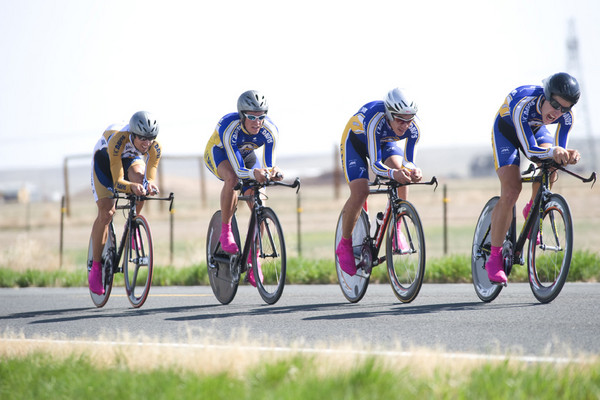
\includegraphics[scale=.54]{bikes.jpg} \\[8mm]
\scalebox{1.5}{\sf David Cherney, Tom Denton,}\\[2mm]
\scalebox{1.5}{\sf Rohit Thomas and Andrew Waldron}
\ \ \ \ \\[2mm]}
 

\date{}

\maketitle

\pagecolor{white}
\phantom{.}\vspace{15cm}

\noindent
Edited by Katrina Glaeser and Travis Scrimshaw\\
First Edition. Davis California, 2013.\\

\noindent
\href{http://creativecommons.org/licenses/by-nc-sa/3.0/deed.en_US}{
\includegraphics[scale=.7]{cc.jpg}}
\begin{tabular}{l}
{\small This work is licensed under a}\\
\href{http://creativecommons.org/licenses/by-nc-sa/3.0/deed.en_US}{\small Creative Commons Attribution-NonCommercial-}\\
\href{http://creativecommons.org/licenses/by-nc-sa/3.0/deed.en_US}{\small ShareAlike 3.0 Unported License.}
\end{tabular}






\newpage


%
\section*{Preface}

This ``book'' grew out of a series of twenty five lecture notes for a sophomore linear algebra class
taught at the University of California, Davis. The audience was primarily engineering students and
students of pure sciences, some of whom may go on to major in mathematics.
It was motivated by the lack of a book that 
 taught students basic structures of linear algebra without overdoing mathematical rigor
 or becoming a mindless exercise in crunching recipes at the cost of fundamental understanding.
In particular we wanted a book that was suitable for all students, not just math majors, that focussed
on concepts and developing the ability to think in terms of abstract structures in order to address the 
dizzying array of seemingly disparate applications that can all actually be addressed with linear algebra methods.

In addition we had practical concerns. We wanted to offer students a online version of the book for free, both because
we felt it our academic duty to do so, but also because we could seamlessly link an online book to a myriad of other 
resources--in particular WeBWorK exercises and videos. We also wanted to make the LaTeX source available to other instructors
so they could easily customize the material to fit their own needs. Finally, we wanted to restructure the way the course 
was taught, by getting the students to direct most of their effort at more difficult problems where they had to think through
concepts,  present well-thought out logical arguments and learn to turn word problems into ones where the usual array of linear algebra recipes could take over.

\subsection*{How to Use the Book}

At the end of each chapter there is a set of review questions. Our students found these very difficult, mostly because they 
did not know where to begin, rather than needing a clever trick. We designed them this way to ensure that students grappled with 
basic concepts. Our main aim was for students to master these problems, so that we could ask similar high caliber problems on midterm and
final examinations. This meant that we did have to direct resources to grading some of these problems. For this we used two tricks.
First we asked students to hand in more problems than we could grade, and then secretly selected a subset for grading.
Second, because there are more review questions than what an individual student could handle, we split the class into groups of three
or four and assigned the remaining problems to them for grading. Teamwork is a skill our students will need in the workplace;
also it really enhanced their enjoyment of mathematics.

Learning math is like learning to play a violin--many ``technical exercises'' are
necessary before you can really make music! Therefore, each chapter has a set of dedicated WeBWorK ``skills problems'' where students can test that they have mastered basic linear algebra skills. The beauty of WeBWorK is that students get instant feedback and
problems can be randomized, which means that although students are working on the same types of problem, they cannot simply 
tell each other the answer. Instead, we encourage them to explain to one another how to do the WeBWorK exercises. 
Our experience is that this way, students can mostly figure out how to do the WeBWorK problems among themselves, freeing up discussion groups and office hours for weightier issues.  Finally, we really wanted our students to carefully read the book. Therefore, each chapter has several very simple WeBWorK ``reading problems''. These appear as links at strategic places. They are very simple problems that can 
answered rapidly if a student has read the preceding text.

\subsection*{The Material}

We believe the entire book can be taught in twenty five fifty minute lectures to a sophomore audience that has been exposed to a one year 
calculus course. Vector calculus is useful, but not necessary preparation for this book, which attempts to be self-contained.
Key concepts are presented multiple times, throughout the book, often first in a more intuitive setting, and then again 
in a definition, theorem, proof style later on. We do not aim for students to become agile mathematical proof writers, but we 
do expect them to be able to show and explain why key results hold. We also often use the review exercises to let students discover
key results for themselves; before they are presented again in detail later in the book. 

Linear algebra courses run the risk of becoming a conglomeration of learn-by-rote recipes involving arrays filled with numbers.
In the modern computer era, understanding these recipes, why they work, and what they are for is more important than ever.
Therefore, we believe it is crucial to change the students' approach to mathematics right from the beginning of the course. Instead of
them asking us ``what do I do here?'', we want them to ask ``why would I do that?'' This means that students need to start to think in terms of
abstract structures. In particular, they need to rapidly become conversant in sets and functions--the first WeBWorK set will help 
them brush up these~skills.

There is no best order to teach a linear algebra course. The book has been written such that instructors can reorder the chapters (using the LaTeX source) in any (reasonable) order and still have a consistent text. We hammer the notions of abstract vectors and linear transformations hard and  early, while at the same time giving students the basic matrix skills necessary to perform computations.
Gaussian elimination is followed directly by an ``exploration chapter'' on the simplex algorithm to open students minds to problems 
beyond standard linear systems ones. Vectors in ${\mathbb R}^n$ and general vector spaces are presented back to back so that students
are not stranded with the idea that vectors are just ordered lists of numbers. To this end, we also labor the notion of all functions from a set to 
the real numbers. In the same vein linear transformations and matrices are presented hand in hand. Once students see that a linear map
is specified by its action on a limited set of inputs, they can already understand what a basis is.
All the while students are studying linear systems and their solution sets, so after determinants are introduced right after  matrices.
This material can proceed rapidly since elementary matrices were already introduced with Gaussian elimination. Only then is a careful 
discussion of spans, linear independence and dimension given to ready students for a thorough treatment of eigenvectors and
diagonalization. The dimension formula therefore appears quite late, since we prefer not to elevate rote computations of column and
row spaces to a pedestal. The book ends with applications--least squares and singular values. These are a fun way to end any lecture course.
It would also be quite easy to spend any extra time on systems of differential equations and simple Fourier transform problems.

\newpage 
\noindent
One possible distribution of twenty five fifty minute lectures might be:
\begin{center}
\begin{tabular}{lr}
Chapter & Lectures\\ \hline
What is Linear Algebra?&1\\
Systems of Linear Equations&3\\
The Simplex Method&1\\
Vectors in Space, $n$-Vectors&1\\
Vector Spaces&1\\
Linear Transformations&1\\
Matrices&3\\
Determinants&2\\
Subspaces and Spanning Sets&1\\
Linear Independence&1\\
Basis and Dimension&1\\
Eigenvalues and Eigenvectors&2\\
Diagonalization&1\\
Orthonormal Bases and Complements&2\\
Diagonalizing Symmetric Matrices&1\\
Kernel, Range, Nullity, Rank&1\\ 
Least Squares and Singular Values&1\\ \hline\end{tabular}
\end{center}

Creating this book has taken the labor of many people. Special  thanks are due to Katrina Glaeser  and Travis Scrimshaw
for shooting many of the videos and LaTeXing their scripts. Rohit Thomas wrote many of the WeBWorK problems. Bruno 
Nachtergaele and Anne Schilling provided inspiration for creating a free resource for all students of linear algebra.
Dan Comins helped with technical aspects. A University of California online pilot grant helped fund the graduate students
who worked on the project. Most of all we thank our students who found many errors in the book and taught us how to teach this material!

Finally, we admit the book's many shortcomings: clumsy writing, low quality artwork and low-tech video material. We welcome
anybody who wishes to contribute new material---WeBWorK problems, videos, pictures---to make this resource a better one and are glad to hear of any typographical errors,
mathematical fallacies, or simply ideas how to improve the book.

\vspace{1cm}

\noindent
David, Tom, and Andrew


%These linear algebra lecture notes are designed to be presented as twenty five, fifty minute lectures
%suitable for sophomores likely to use the material for applications but still requiring
%a solid foundation in this fundamental branch of mathematics. The main idea of the course is
%to emphasize the concepts of vector spaces and linear transformations as mathematical
%structures that can be used to model the world around us. Once ``persuaded'' of this truth, students
%learn explicit skills such as Gaussian elimination and diagonalization in order that vectors and linear transformations
%become calculational tools, rather than abstract mathematics.
%
%In practical terms, the course aims to produce students who can perform computations with large linear systems
%while at the same time understand the concepts behind these techniques. Often-times when a problem can be
%reduced to one of linear algebra it is ``solved''. These notes 
%do not devote much space to applications (there are already a plethora of textbooks with titles involving some
%permutation of the words ``linear'', ``algebra'' and ``applications''). Instead, they attempt to explain the fundamental
%concepts carefully enough that students will realize for their own selves when the particular application they encounter
%in future studies is ripe for a solution via linear algebra.
%
%There are relatively few worked examples or illustrations in these notes, this material is instead covered by a series
%of ``linear algebra how-to videos''. They can be viewed by clicking on the take one icon~\raisebox{-.2cm}{
\includegraphics[scale=.05]{take1.jpg}}.
%The \hyperlink{scripts}{``scripts''} for these movies are found at the end of the notes if students prefer to read this material in a traditional format
%and can be easily reached via the script icon~\raisebox{-.2cm}{
\includegraphics[scale=.05]{script.jpg}}. Watch an introductory video below:
%
%\videoscriptlink{intro.mp4}{Introductory Video}{intro}
%
%The notes are designed to be used in conjunction with a set of online homework exercises which help the students read the
%lecture notes and learn 
%basic linear algebra skills. Interspersed among the lecture notes are links to simple online problems that
%test whether students are actively reading the notes. In addition there are two sets of sample midterm problems with solutions as well
%as a sample final exam. 
%There are also a set of ten online assignments which are usually collected weekly.
%The first assignment is designed to ensure familiarity with some basic mathematic notions (sets, functions, logical quantifiers and basic methods of proof). The remaining nine assignments are devoted to the usual matrix and vector gymnastics expected from 
%any sophomore linear algebra class. These exercises are all available at
%
%\begin{quote}
%\href{\webworkurl}{\webworkurl}
%\end{quote}
%
%\noindent
%Webwork is an open source, online homework system which originated at the University of Rochester. It can efficiently check whether a student
%has answered an explicit, typically computation-based, problem correctly. The problem sets chosen to accompany these
%notes could contribute roughly  20\% of a student's grade, and ensure that basic computational skills are mastered.
%Most students rapidly realize that it is best to print out the Webwork assignments and solve them on paper before 
%entering the answers online. Those who do not tend to fare poorly on midterm examinations. We have found that there 
%tend to be relatively few questions from students in office hours about the Webwork assignments. Instead, by assigning 20\%
%of the grade to written assignments drawn from  problems chosen randomly from the review exercises at the end of each lecture, the
%student's focus was primarily on understanding ideas. They range from simple tests of understanding of the material in the lectures
%to more difficult problems, all of them require thinking, rather than blind application of mathematical ``recipes''. 
%Office hour questions reflected this and offered an excellent chance
%to give students tips how to present written answers in a way that would convince the person grading their work that they deserved full credit!
%
%Each lecture concludes with references to the comprehensive online textbooks of Jim Hefferon and Rob Beezer:
%
%\begin{quote}
%\href{http://joshua.smcvt.edu/linearalgebra/}{http://joshua.smcvt.edu/linearalgebra/}\\[5mm]
%\href{http://linear.ups.edu/index.html}{http://linear.ups.edu/index.html}
%\end{quote}
%and the notes are also hyperlinked to Wikipedia where students can rapidly access further details and background material
%for many of the concepts. Videos of linear algebra lectures are available online from at least two sources:
%\begin{itemize}
%\item The Khan Academy, \\ \href{http://www.khanacademy.org/?video#Linear Algebra}{http://www.khanacademy.org/?video\#Linear Algebra}
%\item MIT OpenCourseWare, Professor Gilbert Strang, \\ \href{http://ocw.mit.edu/courses/mathematics/18-06-linear-algebra-spring-2010/video-lectures/}{http://ocw.mit.edu/courses/mathematics/18-06-linear-algebra-spring\\ -2010/video-lectures/}
%\end{itemize}
%There are also an array of useful commercially available texts. A non-exhaustive list includes
%\begin{itemize}
%\item ``Introductory Linear Algebra, An Applied First Course'', B. Kolman and D. Hill, Pearson 2001.
%\item ``Linear Algebra and Its Applications'', David C. Lay, Addison--Weseley 2011.
%\item ``Introduction to Linear Algebra'', Gilbert Strang, Wellesley Cambridge Press 2009.
%\item ``Linear Algebra Done Right'', S. Axler, Springer 1997.
%\item ``Algebra and Geometry'', D. Holten and J. Lloyd, CBRC, 1978.
%\item ``Schaum's Outline of Linear Algebra'', S. Lipschutz and M. Lipson, McGraw-Hill 2008.
%\end{itemize}
%A good strategy is to find your favorite among these in the University Library.
%
%There are many, many useful online math resources. A partial list is given in Appendix~\ref{othersources}.
%
%Students have also started contributing to these notes. Click \hyperlink{student_creations}{here} to see some of their work.
%
%There are many ``cartoon'' type images for the important theorems and formal\ae\ . In a classroom with a projector, a useful technique for instructors
%is to project these using a computer. They provide a colorful relief for  students from (often illegible) scribbles on a blackboard.
%These can be downloaded at:
%
%\begin{center}
%\href{http://math.ucdavis.edu/~linear/lecture_materials}{Lecture Materials}
%\end{center}
%
%There are still many errors in the notes, as well as awkwardly explained concepts. An army of 400 students, Fu Liu, Stephen Pon and Gerry Puckett have already found
%many of them. Rohit Thomas has spent a great deal of time editing these notes and the accompanying webworks and has improved them immeasurably. 
%Katrina Glaeser and Travis Scrimshaw have spent many hours shooting and scripting the how-to videos and taken these notes to a whole new level!
%Anne Schilling shot a great guest video.
%We also thank Captain Conundrum\index{Captain Conundrum} for providing us his solutions to the sample
%midterm and final questions. The review exercises would provide a better survey of what linear algebra really is if there were more ``applied''
%questions.  We welcome your contributions!
%
%\begin{quote}
%Andrew and Tom.
%\end{quote}

 
\newpage


\tableofcontents











%\chapter{\gaussElimTitle}

\label{gaussElim}

You have seen that systems of linear equations can be written as matrix equations.
You will see that Gaussian elimination is an efficient \gls{shorthand} for (maximally) simplifying a system of linear equations (or matrix equation).

%You might get the feeling that you are learning to do Gaussian elimination only so that you can tell your computer how too do it in the future. There is more than that going on here. Let us foreshadow chapter 3; as we attempt to streamline the process of elimination we will discover the building blocks of matrices. 



%In \Lecture~\ref{warmup}  we looked performed elimination on a system of equations. 
%It was nice to do this elimination by adding subtracting an multiplying wholes equations at a time. 
%Lets do another example with the system
%\begin{eqnarray}
%	x\ +\ y & = & 27\nn \\
%	2x-\ y & = &\  0\nn \,.
%\end{eqnarray}
%Adding the first equation to the second then dividing by 3 gives
%\begin{eqnarray}
%	x\ +\ 0 & = & 9\nn \\
%	2x-\ y & = &\  0\nn \,.
%\end{eqnarray}
%Subtracting rice the first from the second then dividing by $-1$ gives
%\begin{eqnarray}
%	x \phantom{\ +\ y}& = &\  9\nn \\
%	\phantom{x\ +\ }y & = & 18\, .\nn
%\end{eqnarray}
%
%\noindent
%The maximum number of terms have been eliminated from each equation, and the result is an obvious statement of the solution. 
%\\
%
%We also learned to write such a linear system using a matrix and two vectors. In this case the original linear system can be written
%
%\begin{equation*}
%    \begin{pmatrix}
%      1             &1  \\
%      2             &-1
%    \end{pmatrix}
%  \colvec{x \\ y}
%  =
%  \colvec{27 \\ 0}\, .
%\end{equation*}
%
%
%\noindent
%Likewise, the system of equations that we obtained after elimination can be written
%
%\begin{equation*}
%    \begin{pmatrix}
%      1             &0  \\
%      0             &1
%    \end{pmatrix}
%  \colvec{x \\ y}
%  =
%  \colvec{9 \\ 18} \, .
%\end{equation*}
%\\
%
%%\noindent
%By the way, the matrix $$I=    \begin{pmatrix}
%      1             &0  \\
%      0             &1
%    \end{pmatrix}$$ is called the \emph{Identity Matrix}\index{Identity matrix!$2\times2$}.  She will be very important to us. You should check that if $v$ is any vector, then $$Iv=v\, .$$
%    
%Here is a nice way to summarize your goal when performing the process we are calling elimination elimination; manipulate the system of equations until the resulting system can be written as a matrix equation with the identity matrix.

%%%%%%%%%%%%%%%%%%%%%%%%%%%%%%%%%%
\section{Augmented Matrix Notation for Linear Systems}

%A useful shorthand for a  system of linear equations is an \hypertarget{augmented_matrix}{\emph{Augmented Matrix}}\index{Augmented matrix~$2\times2$}. 
We will introduce this notation through examples: 
The linear system 
\begin{eqnarray}
	x\ +\ y & = & 27\nn \\
	2x-\ y & = &\  0\nn \,
\end{eqnarray}
is denoted by the augmented matrix

\[
\begin{amatrix}{2}
1 &1 &27 \\ 2 &-1 & 0
\end{amatrix}
\]

\noindent
This is truly minimalist notation. It is even more minimal then the matrix notation  
\begin{equation*}
    \begin{pmatrix}
      1             &1  \\
      2             &-1
    \end{pmatrix}
  \colvec{x \\ y}
  =
  \colvec{27 \\ 0}\, .
\end{equation*}
All three of the above equations denote the same thing. 


\videoscriptlink{gaussian_elimination_more_background.mp4}{Augmented Matrix Notation}{script_gaussian_elimination_more}

Going up in size,
the system
\begin{eqnarray*}
1x + 3y + 2z + 0w   =9 \\ 
6x + 2y + 0z   -2w  =0  \\
-1x+ 0 y + 1 z + 1w  =3 
\end{eqnarray*}
is denoted by the augmented matrix
\[
\begin{amatrix}{4}
1 & 3 & 2 & 0  & 9 \\ 
6 & 2 & 0  & -2 & 0  \\
-1& 0  & 1  & 1 & 3
\end{amatrix}
\]
%When writing a system of equations one can write out the terms with zero for coefficients or not
%\begin{eqnarray*}
%1x + 3y + 2z  \phantom{+ 0w}   =9 \\ 
%6x + 2y \phantom{ + 0z}   -2w  =0  \\
%-1x  \phantom{+0 y} + 1 z + 1w  =3 
%\end{eqnarray*}
As a matrix equation the system reads
\begin{eqnarray*}
\left(\begin{array}{cccc}
1 & 3 & 2 & 0   \\ 
6 & 2 & 0  & -2   \\
-1& 0  & 1  & 1 
\end{array}\right)
\colvec{ x\\ y\\z\\w}
=\colvec{ 9\\0\\3}
\end{eqnarray*}




Here's the general case:  The number of equations in the linear system is the number of rows $r$ in the augmented matrix, and the number of columns $k$ in the matrix left of the vertical line is the number of unknowns.
\[
\begin{amatrix}{4}
a^1_1 & a^1_2 & \cdots & a^1_k & b^1 \\ 
a^2_1 & a^2_2 & \cdots & a^2_k & b^2 \\ 
\vdots & \vdots & & \vdots & \vdots  \\
a^r_1 & a^r_2 & \cdots & a^r_k & b^r \\ 
\end{amatrix}
\]
Entries left of the divide carry two indices; subscript denotes column number, superscript denotes row number. We emphasize, the superscripts here do not denote exponents.  

%Aside: most people don't like  indexing by superscripts at first. However, kind of index placement will later facilitate Einstein's summation convention, which Einstein himself described as his greatest contribution to the sciences. 

Make sure you can write out the system of equations and the associated matrix equation for any augmented matrix. 
\reading{2}{1}




We now have three ways or writing the same question. 
Lets put them side by side as we solve the system using a nice algebra trick: we will strategically add and subtract equations.

\begin{example}  (how matrix equations and augmented matrices change in elimination)
\begin{eqnarray*}
   \left.
\begin{array}{lcr}
	x\ +\ y & = & 27 \\
	2x-\ y & = &\  0 
     \end{array}
   \right\} 
   \Leftrightarrow
    \begin{pmatrix}
      1             &1  \\
      2             &-1
    \end{pmatrix}
  \colvec{x \\ y}
  =
  \colvec{27 \\ 0}
  \Leftrightarrow
 \begin{amatrix}{2}
1 &1 &27 \\ 2 &-1 & 0
\end{amatrix}
  \end{eqnarray*}
Let the new first equation be the sum of the first and second equations
\begin{eqnarray*}
   \left.
\begin{array}{lcr}
	3x\ +\ 0 & = & 27 \\
	2x-\ y & = &\  0 
     \end{array}
   \right\} 
   \Leftrightarrow
    \begin{pmatrix}
      3             &0  \\
      2             &-1
    \end{pmatrix}
  \colvec{x \\ y}
  =
  \colvec{27 \\ 0}
  \Leftrightarrow
 \begin{amatrix}{2}
3 &0 &27 \\ 2 &-1 & 0
\end{amatrix}
  \end{eqnarray*}
Let the new first equation be the old first equation divided by 3
 \begin{eqnarray*}
   \left.
\begin{array}{lcr}
	x\ +\ 0 & = & 9 \\
	2x-\ y & = &\  0 
     \end{array}
   \right\} 
   \Leftrightarrow
    \begin{pmatrix}
      1             &0  \\
      2             &-1
    \end{pmatrix}
  \colvec{x \\ y}
  =
  \colvec{9 \\ 0}
  \Leftrightarrow
 \begin{amatrix}{2}
1 &0 &9 \\ 2 &-1 & 0
\end{amatrix}
  \end{eqnarray*}
Let the new second equation be the old second equation minus two times the first equation 
\begin{eqnarray*}
   \left.
\begin{array}{lcr}
	x\ +\ 0 & = & 9 \\
	0-\ y & = &\  -18
     \end{array}
   \right\} 
   \Leftrightarrow
    \begin{pmatrix}
      1             &0  \\
      0             &-1
    \end{pmatrix}
  \colvec{x \\ y}
  =
  \colvec{9 \\ -18}
  \Leftrightarrow
 \begin{amatrix}{2}
1 &0 &9 \\ 0 &-1 & -18
\end{amatrix}
  \end{eqnarray*}
Let the new  second equation be the old second equation divided by -1
\begin{eqnarray*}
   \left.
\begin{array}{lcr}
	x + 0 & = & \ 9 \\
	0 + y & = &  18
     \end{array}
   \right\} 
   \Leftrightarrow
    \begin{pmatrix}
      1             &0  \\
      0             &1
    \end{pmatrix}
  \colvec{x \\ y}
  =
  \colvec{9 \\ 18}
  \Leftrightarrow
 \begin{amatrix}{2}
1 &0 &9 \\ 0 &1 & 18
\end{amatrix}
  \end{eqnarray*}
\end{example}
Did you see what the strategy was? To eliminate $y$ from the first question and then eliminate $x$ from the second. The result was a plain statement of the solution. But the quantity of writing here was atrocious. 

Here is the big idea: 
Everywhere in the the instructions we can replace the word ``equation" with the word ``row" and interpret the instructions as telling us what to do with the augmented matrix instead of the system of equations.
The result is a process called {\it Gaussian elimination}\index{Gaussian elimination}: 
%
%\begin{example} of Gaussian elimination
%\begin{eqnarray*}
% \begin{amatrix}{2}
%1 &1 &27 \\ 2 &-1 & 0
%\end{amatrix}
%  \end{eqnarray*}
%Let the new first row be the sum of the first and second rows
%\begin{eqnarray*}
% \begin{amatrix}{2}
%3 &0 &27 \\ 2 &-1 & 0
%\end{amatrix}
%  \end{eqnarray*}
%Let the new first row be the old first row divided by 3
% \begin{eqnarray*}
% \begin{amatrix}{2}
%1 &0 &9 \\ 2 &-1 & 0
%\end{amatrix}
%  \end{eqnarray*}
%Let the new second row be the old second row minus two times the first row 
%\begin{eqnarray*}
% \begin{amatrix}{2}
%1 &0 &9 \\ 0 &-1 & -18
%\end{amatrix}
%  \end{eqnarray*}
%Let the new  second row be the old second row divided by -1
%\begin{eqnarray*}
% \begin{amatrix}{2}
%1 &0 &9 \\ 0 &1 & 18
%\end{amatrix}
%  \end{eqnarray*}
%The solution can be read off very quickly, and the notation was very minimal. 
%\end{example}
% At each step, the augmented matrices encode systems of equations which have the same solutions. Lets make this idea more formal, and introduce some notation to convey the idea.
%

%%%%%%%%%%%%%%%%%%%%%%%%%%%%%%%%%%%%
%%%%%%%%%%%%%%%%%%%%%%%%%%%%%%%%%%%%

\section{Equivalence and the Act of Solving}


%Two augmented matrices corresponding to linear systems 
%%{\it that actually have solutions} %cmon, this idea has not even been introduced
%are said to be \hypertarget{roweq}(row) 
%\emph{equivalent}\index{Row equivalence} if they have the \emph{same} solutions.
%To denote this 

We introduce the symbol $\sim$ which is called ``tilde" but should be read as  ``is equivalent to''. For example we found above that
\[
\begin{amatrix}{2}
1 &1 &27 \\ 2 &-1 &0
\end{amatrix}
\sim
\begin{amatrix}{2}
1 &0 &9 \\ 2 &-1 & 0
\end{amatrix}
\sim
\begin{amatrix}{2}
1 & 0&9 \\   0& 1 & 18
\end{amatrix}
\]
and certainly the last of these is our favorite!
\videoscriptlink{gaussian_elimination_background.mp4}{Equivalence Example}{script_gaussian_elimination_background}

%\videoscriptlink{gaussian_elimination_3_3_example.mp4}{A $3 \times 3$ example}{scripts_gaussian_elimination_3_3_example}

Setting up a string of equivalences like this is a means of solving a system of linear equations. This is the main idea of chapter 2.

\begin{example} (Using Gaussian elimination to solve a system of linear equations)
\begin{eqnarray*}
   \left.
\begin{array}{lcr}
	x +\ y & = & 5 \\
	x + 2y & = &\  8
     \end{array}
   \right\} 
   \Leftrightarrow
\begin{amatrix}{2}
1 &1 &5 \\ 1 &2 & 8
\end{amatrix}
\sim
\begin{amatrix}{2}
1 &1 &5 \\ 0 &1 & 3
\end{amatrix}
\sim
\begin{amatrix}{2}
1 &0 &2 \\ 0 &1 & 3
\end{amatrix}
\Leftrightarrow
\left\{
\begin{array}{lcr}
	x + 0 & = & 2 \\
	 0 + y & = &\  3
     \end{array}
   \right.
\end{eqnarray*}  
Note that we used the top left $1$ to make the bottom left entry zero. For this reason we call that number a pivot; imagine a wiper blade hanging down form the top left slot wiping the lower left slot away. Similarly the bottom right slot was used to wipe away the top right slot, so it is called a pivot. 
\end{example}

This {\it pivot} jargon is helpful for describing the goings on in Gaussian elimination. Be sure you understand the idea before moving on. 

%%%%%%%%%%%%%%%%%%%%%%%%%%%%%%%%%%%

\section{Reduced Row Echelon Form}
For a system of two linear  equations, the goal in Gaussian elimination is to have the part of the augmented matrix left of the dividing line become the matrix
 $$I=    \begin{pmatrix}
      1             &0  \\
      0             &1
    \end{pmatrix}$$ 
called the \emph{Identity Matrix}\index{Identity matrix!$2\times2$}, since this would give the simple statement of a solution $x=a,y=b$. The situation is similar for larger systems of equations.
\reading{2}{2} %a 3x3 example with one solution>



\noindent
This can't always be done.

\begin{example} (Redundant equations)
 \begin{eqnarray*}
   \left.
\begin{array}{lcr}
	\ x + \ y & = & 2 \\
	2x + 2y & = &  4
     \end{array}
   \right\} 
   \Leftrightarrow
\begin{amatrix}{2}
1 &1 &2 \\ 2 &2 & 4
\end{amatrix}
\sim
\begin{amatrix}{2}
1 &1 &2 \\ 0 &0 & 0
\end{amatrix}
%\sim
%\begin{amatrix}{2}
%1 &0 &2 \\ 0 &1 & 3
%\end{amatrix}
\Leftrightarrow
\left\{
\begin{array}{lcr}
	x + y & = & 2 \\
	 0 + 0 & = &  0
     \end{array}
   \right.
\end{eqnarray*}  
This example demonstrates if one equation is a multiple of the other the identity matrix can not be a reached. This is because the first step in elimination will make the second row a row of zeros. Notice that solutions still exists $x=1,y=1$ is a solution. The last augmented matrix here is in RREF.
\end{example}

\begin{example} (Inconsistent equations)
 \begin{eqnarray*}
   \left.
\begin{array}{lcr}
	\ x + \ y & = & 2 \\
	2x + 2y & = &  5
     \end{array}
   \right\} 
   \Leftrightarrow
\begin{amatrix}{2}
1 &1 &2 \\ 2 &2 & 5
\end{amatrix}
\sim
\begin{amatrix}{2}
1 &1 &2 \\ 0 &0 & 1
\end{amatrix}
%\sim
%\begin{amatrix}{2}
%1 &0 &2 \\ 0 &1 & 3
%\end{amatrix}
\Leftrightarrow
\left\{
\begin{array}{lcr}
	x + y & = & 2 \\
	 0 + 0 & = &  1
     \end{array}
   \right.
\end{eqnarray*}  
This system of equation has a solution if there exists two numbers $x$, and $y$ such that $0+0=1$. That is a tricky way of saying there are no solutions. The last form of the augmented matrix here is in RREF.
\end{example}


\begin{example} (Silly order of equations)\\
A robot might make the following mistake
 \begin{eqnarray*}
   \left.
\begin{array}{lcr}
	0x +  \ y & = & -2 \\
	\ x + y & = &  7
     \end{array}
   \right\} 
   \Leftrightarrow 
\begin{amatrix}{2}
0 &1 & -2\\ 1 &1 & 7
\end{amatrix}
\sim \cdots
\end{eqnarray*}  
and then give up because the the upper left slot can not function as a pivot since the 0 that lives there can not be used to eliminate the zero below it. Of course, the right thing to do is to change the order of the equations before starting
 \begin{eqnarray*}
   \left.
\begin{array}{lcr}
	\ x + y & = &  7
	\\
	0x +  \ y & = & -2 
	     \end{array}
   \right\} 
   \Leftrightarrow
\begin{amatrix}{2}
1 &1 & 7\\ 0 &1 & -2
\end{amatrix}
\sim 
\begin{amatrix}{2}
1 &0 & 9\\ 0 &1 & -2
\end{amatrix}
\Leftrightarrow
\left\{
\begin{array}{lcr}
	x + 0 & = & 9 \\
	 0 + y & = & -2
     \end{array}
   \right.
\end{eqnarray*}  
The third appearance of an augmented matrix here is RREF of the first, and second. That is to say, you can swap rows on your way to RREF.
\end{example}



For larger systems of matrices, these three kinds of problems are the obstruction to obtaining the identity matrix, and hence to a simple statement of a solution in the form $x=a,y=b,...$. 
What can we do to maximally simplify a system of equations in general?
We can do three things corresponding to exchanging the order of equations, multiplying one equation by a constant or adding equations:
\begin{itemize}
\item (Row Swap) Exchange any two rows.
\item (Scalar Multiplication) Multiply any row by a non-zero constant.
\item (Row Sum) Add a multiple of one row to another row.
\end{itemize}
These are called the \emph{Elementary Row Operations}\index{EROs}, or EROs for short. They are the  subject of the next lecture. 
They can be used to achieve \emph{Reduced Row Echelon Form}\index{Reduced row echelon form} (RREF), the maximally simplified augmented matrix, which typically looks like 
\[
\begin{amatrix}{7}
1       	& * & 0		& * & 0		& \cdots& 0		& b^1 \\ 
0	        & 0 & 1		& * & 0		& \cdots& 0		& b^2 \\
0		& 0& 0		& 0 & 1		& \cdots& 0		& b^3 \\  
\vdots  	& \vdots& \vdots	&   & \vdots	& 	& 0			& \vdots \\  
		& &			&  &			&      & 1			& b^k \\  
0		& 0 & 0		& 0 & 0		& \cdots& 0 		& b^{k+1} \\ 
\vdots  	& \vdots & \vdots	&  \vdots & \vdots	& 	& \vdots		& \vdots \\  
0		&  0 & 0		& 0 & 0		& \cdots& 0		& b^r \\ 
\end{amatrix}
\]

%The first non-zero entry in each row is called the \emph{pivot}\index{Pivot}.    
\noindent
The asterisks denote the possibility of arbitrary numbers. (For e.g. 1 in the redundant equations example.)  
If any of the numbers $b^{k+1},\dots b^r$ are non-zero then the system of equations is inconsistent and has no solutions. 


It is essential to be able to visualize how 
RREF can be obtained using (only) elementary row operations in the most general case:
\begin{itemize}
\item Make the leftmost nonzero entry in the top row 1 by multiplication.  
\item Then use that 1 as a pivot to eliminate everything below it. 
\item Then go to the next row and make the leftmost non zero entry 1. 
\item Then use that 1 as a pivot to eliminate everything below {\it and above it}! 
\item Then go to the next row and make the leftmost nonzero entry 1... etc
\end{itemize}
Note that this is not the only way to get to RREF. You might, for example, begin by eliminating everything below the top left entry before setting it to one. 

\videoscriptlink{gaussian_elimination_Beginner_Elimination.mp4}{Beginner Elimination}{script_gaussian_elimination_more}

\noindent
The following properties fully describe  RREF.

\begin{enumerate}
\item  In every row  the left most non-zero entry is  $1$ (and is called a pivot).

\item The pivot of any given row is always to the right of the pivot of the row above it.

\item The pivot is the only non-zero entry in its column.
\end{enumerate}

\begin{example} (Augmented matrix in RREF)
$$
\begin{amatrix}{3} 
1 & 0 & 7 & 0 \\ 
0 & 1 & 3 & 0 \\
0 & 0 & 0 & 1 \\
0 & 0 & 0 & 0 \\
\end{amatrix}
$$
\end{example}

\begin{example} (Augmented matrix NOT in RREF)
$$
\begin{amatrix}{3} 
1 & 0 & 3 & 0 \\ 
0 & 0 & 2 & 0 \\
0 & 1 & 0 & 1 \\
0 & 0 & 0 & 1 \\
\end{amatrix}
$$
Actually, this NON-example breaks all three of the rules!
\end{example}


The reason we need the asterisks in the general form of RREF:
it is not necessary for every column to have a pivot as demonstrated in the ``augmented matrix in RREF" and ``redundant equations" examples above. 
Actually, in full generality where we have asterisks one can have multiple columns with no pivot as one would have in the following

\begin{example} (Consecutive  columns with no pivot in RREF)
 \begin{eqnarray*}
   \left.
\begin{array}{lcr}
	\ x \ + \ y + \ z +  0w & = & 2 \\
	2x + 2y +2z+2w & = &  4
     \end{array}
   \right\} 
   \Leftrightarrow
\begin{amatrix}{4}
1 &1 &1 & 0 &2 \\ 
2 &2 &2 & 1 & 4
\end{amatrix}
\\
\sim
\begin{amatrix}{4}
1 &1 &1 & 0 &2 \\ 
0 &0 &0 & 1 & 0
\end{amatrix}
\Leftrightarrow
\left\{
\begin{array}{lcr}
	x + y +z& = & 2 \\
	 w & = &  0
     \end{array}
   \right.
\end{eqnarray*}  
Note that there was no hope of reaching the identity matrix just because of the shape of the augmented matrix we started with. 
\end{example}


\videoscriptlink{gaussian_elimination_Advanced_Elimination.mp4}{Advanced Elimination}{script_gaussian_elimination_more}



\section{Solution Sets}
%While RREF is not always pretty, it is certainly useful. 
%Our goal  is to solve systems of linear equations. 
RREF represents a maximally simplified version of the original system of equations in the following sense: 
\begin{itemize}
\item As many coefficient of the variables have been set to zero as is possible 
\item As many coefficients of variables have been set to 1 as possible.
\end{itemize}
It is easier to read off solutions from the maximally simplified equations than from the original equations, even when there are infinitely many solutions.

\begin{example}
 \begin{eqnarray*}
\left.
\begin{array}{lcr}
	x  +y    \phantom{+ z}  + 5w & ~  = 1 \\
	\phantom {x+}  \ y  \phantom{+z}   + 2 w & = 6 \\
	\phantom{x+y+} z+         4w & = 8
\end{array}
 \right\}
 \Leftrightarrow
 \begin{amatrix}{4} 
1 & 1 & 0 & 5 & 1 \\ 
0 & 1 & 0 & 2 & 6 \\
0 & 0 & 1 & 4 & 8 
\end{amatrix}
\sim
 \begin{amatrix}{4} 
1 & 0 & 0 & 3 & -5 \\ 
0 & 1 & 0 & 2 & 6 \\
0 & 0 & 1 & 4 & 8 
\end{amatrix}
\\
\Leftrightarrow
\left\{
\begin{array}{lcr}
	x \phantom{+y    + z}  + 3w & ~ \ = -5 \\
	\phantom {x+}   y \, \phantom{+z}  \ + 2 w & = 6 \\
	\phantom{x+y+} z+         4w & = 8
     \end{array}
     \right.
\end{eqnarray*}
In this case, we say that $x,y$, and $z$ are {\it pivot variables}\index{pivot variables} because they appear with pivots as coefficients. Since $w$ never appears with a pivot as a coefficient, 
we say that it is not a pivot variable. %We call it a free variable. 
One way to express the solutions to this system of equations is to put all the pivot variables on one side and all the {\it non-pivot variables}\index{non-pivot variables} on the other side. It is also nice to add the ``freebee equation" $w=w$ to obtain the system
\begin{eqnarray*}
\left.
\begin{array}{lcr}
	x & = -5 -3w \\
	 y  & = 6 -2w\\
	 z & = 8-4w \\
	w & =\phantom{8-4}w          
     \end{array}
     \right\}
     \Leftrightarrow
\colvec{x\\y\\z\\w} = \colvec{-5\\6\\8\\0} + w\colvec{-3\\-2\\-4\\1}
\end{eqnarray*}
where we have written the solution to the corresponding matrix problem. There are infinitely many solutions, one for each value of $z$. We call the collection of all solutions {\it the solution set}\index{solution set}\index{solution set} It is easy to check that the solution corresponding to $w=0$ really does fit into the matrix equation. 
\end{example}


The last example demonstrated the \hypertarget{standard approach}{{\it standard approach}} to solving a system of linear equations in its entirety: write the augmented matrix, obtain RREF, return to the system of equations, and express the non-pivot variables in terms of the pivot variables. 
There are always exactly enough non-pivot variables to index your solutions. 
In any approach, the variables which are not expressed in terms of the other variables are called the {\it free variables}\index{free variables}. The standard approach is to use the non-pivot variables as free variables.

%vid for this?! 
Non-standard approach: solve for $w$ in terms of $z$ and substitute into the other equations. You now have an expression for each component in terms of $z$. But why pick $z$ instead of $y$ or $x$? (or $x+y$?) The standard approach feels natural, and that is why it became the standard.

When you see a RREF augmented matrix with two columns that have no pivot, you know there will be two free variables. 

\begin{example}
 \begin{eqnarray*}
 \begin{amatrix}{4} 
1 & 0 & 7 & 0 & 4 \\ 
0 & 1 & 3 & 4 & 1 \\ 
0 & 0 & 0 & 0 & 0 \\ 
0 & 0 & 0 & 0 & 0 \\ 
\end{amatrix}
\Leftrightarrow
\left\{
\begin{array}{lcr}
	x \phantom{+y}    + 7z  \phantom{+w} & = 4 \\
	\phantom {x+}   y + 3z  {+4w} & = 1 \\
	%\phantom{x+y+z+}          w & = 2
     \end{array}
     \right.
\end{eqnarray*}  
Expressing the pivot variables in terms of the non-pivot variables, and using two freebee equations gives
\begin{eqnarray*}
\left.
\begin{array}{lcr}
	x & = 4 -7z \\
	 y  & = 1 -3z-4w\\
	 z         & = z\\
	w & =w          
     \end{array}
     \right\}
     \Leftrightarrow
\colvec{x\\y\\z\\w} = \colvec{4\\1\\0\\0} + z\colvec{-7\\-3\\1\\0} + w\colvec{0\\-4\\0\\1}
\end{eqnarray*}
There are infinitely many solutions. One solution for each pair of numbers $z,w$. 
\end{example}
You can imagine having three, four, or fifty-six non-pivot columns and the same number of free variables indexing your solutions set. You need to become very adept at reading off solutions of linear systems from the RREF
of their augmented matrix. 

\videoscriptlink{solution_sets_for_systems_example.mp4}{Solution set in set notation}{solution_sets_for_systems_of_linear_equations_example}

\videoscriptlink{elementary_row_operations_worked_examples.mp4}{\hspace{-8mm}Worked examples of Gaussian elimination\hspace{-8mm}}{scripts_elementary_row_operations_worked_examples}


%This example emphasizes different aspects.
%\begin{example}
%$$
%\begin{amatrix}{5} 
%1 & 1 & 0 & 1 & 0 & 1\\ 
%0 & 0 & 1 & 2 & 0 & 2\\ 
%0 & 0 & 0 & 0 & 1 & 3\\ 
%0 & 0 & 0 & 0 & 0 & 0
%\end{amatrix}\, .
%$$
%Here we were not told the names of the variables, so lets just call them $x_1,x_2,x_3,x_4,x_5$.
%(There are always as many of these as there are columns in the matrix before the vertical line; the number of rows,
%on the other hand is the number of linear equations.)
%
%To begin with we immediately notice that there are no pivots in the second and fourth columns so, as per the standard approach, we will be all variables in terms of $x_2$ and $x_4$. 
%Next we see from the second last row that $x_5=3$. The second row says 
%$x_3=2-2x_4=2-2 x_2$.
%The top row then gives $x_1=1-x_2-x_4=1-x_1-x_2$. Again we can write this solution as a vector
%$$
%\colvec{1\\0\\2\\0\\3}+x_1\colvec{-1\\1\\0\\0\\0}+x_2\colvec{-1\\0\\-2\\1\\0}\, .
%$$
%Observe, that since no variables were given at the beginning, we can use any symbols instead of $x_1$ and $x_2$. For example lower case greek letter lambda:
%$$
%\colvec{1\\0\\2\\0\\3}+\lambda_1\colvec{-1\\1\\0\\0\\0}+\lambda_2\colvec{-1\\0\\-2\\1\\0}\, .
%$$
%As a challenge, look carefully at this solution and make sure you can see how every part of it comes from
%the original augmented matrix without every having to reintroduce variables and equations.
%\end{example}
%
%




%\begin{theorem}
%Every augmented matrix is row-equivalent to a \emph{unique} augmented matrix in reduced row echelon form.
%\end{theorem}
%
%\noindent
%In \Lecture~\ref{elemRowOpsPath}, we will see why this is true.

%\section*{Uniqueness of RREF}
%
%\begin{theorem}\label{GJEunique} Gauss-Jordan Elimination produces a unique augmented matrix in RREF.
%\end{theorem}
%
%\begin{proof}
%Suppose Alice and Bob compute the RREF for a linear system but get different results, $A$ and $B$.  Working from the left, discard all columns except for the pivots and the first column in which $A$ and $B$ differ.  By \hyperref[colremove]{Review Problem~\ref{colremove}}, removing columns does not affect row equivalence.  Call the new, smaller, matrices $\hat{A}$ and $\hat{B}$.  The new matrices should look this: $$\hat{A}=\begin{amatrix}{1}
%I_N & a\\
%0 & 0
%\end{amatrix} \mbox{ and } \hat{B}=\begin{amatrix}{1}
%I_N & b\\
%0 & 0
%\end{amatrix}\, ,$$ where $I_N$ is an $N\times N$ identity matrix and $a$ and $b$ are vectors.
%
%Now if $\hat{A}$ and $\hat{B}$ have the same solution, then we must have $a=b$.  But this is a contradiction!  Then $A=B$.
%\end{proof}
%
%\videoscriptlink{elementary_row_operations_proof.mp4}{Explanation of the proof}{scripts_elementary_row_operations_proof}


%\References{
%Hefferon, Chapter One, Section 1
%\\
%Beezer, Chapter SLE, Section RREF
%\\
%Wikipedia, \href{http://en.wikipedia.org/wiki/Row_echelon_form}{Row Echelon Form}}

%\newpage

\section{Review Problems}




\begin{enumerate}

\item Let $D=\begin{pmatrix}
\lambda_1 & \mc0 \\
\mc0 & \lambda_2 \\
\end{pmatrix}$.
\begin{enumerate}
\item Write $D$ in terms of the vectors $e_1$ and $e_2$, and their transposes.
\item Suppose $P=\begin{pmatrix}
a & b \\
c & d \\
\end{pmatrix}$ is invertible.  Show that $D$ is similar to
\[
M=\frac{1}{ad-bc}\begin{pmatrix}
\lambda_1ad-\lambda_2bc & -(\lambda_1-\lambda_2)ab \\[1mm]
(\lambda_1-\lambda_2)cd & -\lambda_1bc + \lambda_2ad
\end{pmatrix}.
\]
\item Suppose the vectors $\rowvec{a,b}$ and $\rowvec{c,d}$ are orthogonal.  What can you say about $M$ in this case? (Hint: think about what \(M^T\) is equal to.)
\end{enumerate}

\phantomnewpage

\item \label{orthogprob} Suppose $S=\{v_1, \ldots, v_n \}$ is an \emph{orthogonal} (not orthonormal) basis for~$\Re^n$.  Then we can write any vector $v$ as $v=\sum_ic^iv_i$ for some constants $c^i$.  Find a formula for the constants $c^i$ in terms of $v$ and the vectors in~$S$.

\Videoscriptlink{orthonormal_bases_hint.mp4}{Hint}{scripts_orthonormal_bases_hint}
\phantomnewpage

\item \label{orthogprojprob} Let $u,v$ be linearly independent vectors in $\Re^3$, and $P=\spa \{ u,v\}$ be the plane spanned by $u$ and $v$.  
\begin{enumerate}
\item Is the vector $v^\bot := v-\frac{u\cdot v}{u\cdot u}u$ in the plane $P$?
\item  What is the (cosine of the) angle between $v^\bot$ and $u$?
\item %Given your solution to the above, 
How can you find a third vector perpendicular to both $u$ and $v^\bot$?
\item  Construct an orthonormal basis for $\Re^3$ from $u$ and $v$.
\item  Test your abstract formul\ae\ starting with 
\[
u=\rowvec{1 , 2 , 0} \text{ and } v=\rowvec{0 , 1 , 1}.
\]
\end{enumerate}

\Videoscriptlink{orthonormal_bases_hint3.mp4}{Hint}{scripts_orthonormal_bases_hint3}

\phantomnewpage



\item Find an orthonormal  basis for $\Re^4$ which includes $(1,1,1,1)$ using the following procedure:\\
\begin{enumerate} 
\item Pick a vector perpendicular to the vector 
$$v_1 =\colvec{1\\1\\1\\1}$$ from the solution set of the matrix equation $$v_1^Tx=0\, .$$ Pick the vector $v_2$ obtained from the standard Gaussian elimination procedure which is the coefficient of $x_2$.
\item Pick a vector perpendicular to both $v_1$ and $v_2$ from the solutions set of the matrix equation $$\colvec{v_1^T\\[1mm]v_2^T}x=0\, .$$ Pick the vector $v_3$ obtained from the standard Gaussian elimination procedure with $x_3$ as the coefficient. 
\item Pick a vector perpendicular to $v_1,v_2,$ and $v_3$ from the solution set of the matrix equation $$\colvec{v_1^T\\[1mm]v_2^T\\[1mm]v_3^T}x=0\, .$$  Pick the vector $v_4$ obtained from the standard Gaussian elimination procedure with $x_3$ as the coefficient. 
\item Normalize the four vectors obtained   above.
\end{enumerate}


\item Use the inner product $$f\cdot g := \int_0^1 f(x)g(x)dx$$  on the vector space $V={\rm span} \{1,x,x^2,x^3\}$ to perform the Gram-Schmidt procedure on the set of vectors $\{1,x,x^2,x^3\}$. 

\item Use the inner product $$f\cdot g := \int_0^{2\pi} f(x)g(x)dx$$  on the vector space $V={\rm span} \{\sin(x),\sin(2x),\sin(3x) \}$ to perform the Gram-Schmidt procedure on the set of vectors $\{\sin(x),\sin(2x),\sin(3x) \}$. \\
Try to build an orthonormal basis for the vector space $$\spa \{ \sin(nx)~| ~n\in \N \}\, .$$
%What do you suspect about the vector space $\spa \{ \sin(nx)~| ~n\in \N \}$?\\
%What do you suspect about the vector space $\spa \{ \sin(ax)~|~ a \in \Re \}$?
\item 
\begin{enumerate}
\item
Show that if $Q$ is an orthogonal $n\times n$ matrix, then $$u\dotprod v = (Qu)\dotprod (Qv)\, ,$$ for any $u,v\in \Re^n$. That is, $Q$ preserves the inner product. 
\item Does $Q$ preserve the outer product? 
\item  If the set of vectors $\{ u_1,\dots,u_n\}$ is orthonormal and $\{ \lambda_1,\cdots,\lambda_n\}$ is a set of numbers, 
then what are the eigenvalues and eigenvectors of the matrix
$M=\sum_{i=1}^n \lambda_i u_i u_i^T$? 
\item How would the eigenvectors and eigenvalues of this matrix change if we replaced  $\{ u_1,\dots,u_n\}$ by $\{ Qu_1,\dots,Q u_n\}$?
\end{enumerate}


\item Carefully write out the Gram-Schmidt procedure for the set of vectors 
$$\left\{ \colvec{1\\1\\1}, \colvec{1\\-1\\1}, \colvec{1\\1\\-1} \right\} \, .$$ Is it possible to rescale the second vector obtained in the procedure to a vector with integer components? 


\item 
\label{basisortho}
\begin{enumerate}
\item Suppose $u$ and $v$ are linearly independent.  Show that $u$ and $v^\perp$ are also linearly independent.  Explain why $\{u, v^\perp\}$ is a basis for $\spa \{u,v\}$.



\Videoscriptlink{gram_schmidt_and_orthogonal_complements_hint.mp4}{Hint}{gram_schmidt_and_orthogonal_complements_hint}

\item Repeat the previous problem, but with three independent vectors $u,v,w$
 where $v^\perp$ and $w^\perp$ are as defined by the Gram-Schmidt procedure. 
\end{enumerate}

\phantomnewpage


\item \label{QRprob} Find the $QR$ factorization of
$$
M=\begin{pmatrix}1&0&\phantom{\!-}2\\-1&2&0\\-1&-2&2
\end{pmatrix}\, .
$$

\phantomnewpage

\item Given any three vectors $u,v,w$, when do $v^\perp$ or $w^\perp$ of the Gram--Schmidt procedure vanish?

\phantomnewpage

\item For $U$ a subspace of $W$, use the subspace theorem to check that $U^\perp$ is a subspace of $W$.

\phantomnewpage


\phantomnewpage

\item %(Extra Credit) 
Let $S_n$ and $A_n$ define the space of $n \times n$ symmetric and anti-symmetric matrices, respectively. These are subspaces of the vector space $M^n_n$ of all $n\times n$ matrices. What is $\dim M^n_n$, $\dim S_n$, and $\dim A_n$? Show that $M^n_n = S_n + A_n$. Define an inner product on square matrices
$$
M\cdot N ={\rm tr} MN\, .
$$
Is $A_n^{\perp}=S_n$? Is $M^n_n = S_n \oplus A_n$?

%\emph{Hint: Note that $\dim S_n = \dim U_n$ where $U_n$ is the vector space of all $n \times n$ upper triangular matrices, and also note that $\dim A_n = \dim \widetilde{U}_n$ where $\widetilde{U}_n$ is the vector space of all strictly $n \times n$ upper triangular matrices (\emph{i.e.} the diagonal entries are all 0).}

\item The vector space $V={\rm span} \{ \sin(t),\sin(2t), \sin(3t) , \sin(3t)\}$ has an inner product: 
$$f\cdot g:=\int _0^{2\pi}f(t)g(t) dt\, .$$ Find the orthogonal compliment to $U={\rm span} \{ \sin(t)+\sin(2t) \}$ in $V$. Express $\sin(t)-\sin(2t)$ as  the sum of vectors from $U$ and $U^\perp$.

\end{enumerate}

\phantomnewpage

\newpage


%To do: write about vector space closure 
\chapter{\luDecompTitle}
\label{LUdecomp}

Certain matrices are easier to work with than others.  In this section, we will see how to write any square\footnote{The case where $M$ is not square is dealt with at the end of the lecture.} matrix $M$ as the product of two simpler matrices.  We will write $$M=LU\, ,$$ where:
\begin{itemize}
\item $L$ is \emph{lower triangular}\index{Lower triangular matrix}.  This means that all entries above the main diagonal are zero.  In notation,
$L=(l^i_j)$ with $l^i_j=0$ for all $j>i$.
\[L=\begin{pmatrix}
l^1_1 & 0 & 0 & \cdots \\
l^2_1 & l^2_2 & 0 & \cdots \\
l^3_1 & l^3_2 & l^3_3 & \cdots \\
\vdots & \vdots & \vdots & \ddots \\
\end{pmatrix}
\]

\item $U$ is \emph{upper triangular}\index{Upper triangular matrix}.  This means that all entries below the main diagonal are zero.  In notation,
$U=(u^i_j)$ with $u^i_j=0$ for all $j<i$.
\[U=\begin{pmatrix}
u^1_1 & u^1_2 & u^1_3 & \cdots \\
0 & u^2_2 & u^2_3 & \cdots \\
0 & 0 & u^3_3 & \cdots \\
\vdots & \vdots & \vdots & \ddots \\
\end{pmatrix}
\]
\end{itemize}
$M=LU$ is called an \emph{$LU$ decomposition}\index{LU@$LU$ decomposition} of $M$.

This is a useful trick for  computational reasons; it is much easier to compute the inverse of an upper or lower triangular matrix than general matrices.  Since inverses are useful for solving linear systems, this makes solving any linear system associated to the matrix much faster as well.  The determinant---a very important quantity associated with any square matrix---is very easy to compute for triangular matrices.

\begin{example}
Linear systems associated to upper triangular matrices are very easy to solve by back substitution.
\[
\begin{amatrix}{2}
a & b & 1 \\
0 & c & e \\
\end{amatrix} \ \Rightarrow \ y=\frac{e}{c}\, , \quad x=\frac{1}{a}\left(1-\frac{be}{c}\right)
\]

\[
\begin{amatrix}{3}
1 & 0 & 0 & d \\
a & 1 & 0 & e \\
b & c & 1 & f \\
\end{amatrix} \Rightarrow x=d\, , \qquad y=e-ad\, , \qquad z=f-bd-c(e-ad)
\]
For lower triangular matrices, \emph{back} substitution\index{Back substitution} gives a quick solution; for upper triangular matrices, \emph{forward} substitution\index{Forward substitution} gives the solution.
\end{example}





\section{Using $LU$ Decomposition to Solve Linear Systems}

Suppose we have $M=LU$ and want to solve the system
\[
MX=LUX=V.
\]

\begin{itemize}
\item{Step 1:} Set $W=\colvec{u\\v\\w}=UX$.  

\item{Step 2:} Solve the system $LW=V$.  This should be simple by forward substitution since $L$ is lower triangular.  Suppose the solution to $LW=V$ is $W_0$.  

\item{Step 3:} Now solve the system $UX=W_0$.  This should be easy by backward substitution, since $U$ is upper triangular.  The solution to this system is the solution to the original system.
\end{itemize}
We can think of this as using the matrix $L$ to perform row operations on the matrix $U$ in order to solve the system; this idea also appears in the  study of determinants.

%\href{\webworkurl ReadingHomework11/1/}{Reading homework: problem 11.1}
\reading{11}{1}

\begin{example}
Consider the linear system:
\[
      \begin{linsys}{4}
            6x & +&18y & +&3z         &=& 3  \\[1mm]
            2x & +&12y & +&z	    &=& 19 \\[1mm]
            4x & +&15y & +&3z         &=& 0  
      \end{linsys}
\]

An $LU$ decomposition for the associated matrix $M$ is:
\[
\begin{pmatrix}
6 & 18 & 3 \\
2 & 12 & 1 \\
4 & 15 & 3 
\end{pmatrix} =
\begin{pmatrix}
3 & 0 & 0 \\
1 & 6 & 0 \\
2 & 3 & 1 
\end{pmatrix}
\begin{pmatrix}
2 & 6 & 1 \\
0 & 1 & 0 \\
0 & 0 & 1 
\end{pmatrix}.
\]

\begin{itemize}
\item{Step 1:} \hypertarget{LUproc}{Set} $W=\colvec{u\\v\\w}=UX$.  

\item{Step 2:} Solve the system $LW=V$:

\[
\begin{pmatrix}
3 & 0 & 0 \\
1 & 6 & 0 \\
2 & 3 & 1 
\end{pmatrix}
\colvec{u\\v\\w} =
\colvec{3\\19\\0}
\]

By substitution, we get $u=1$, $v=3$, and $w=-11$.  Then 
\[W_0=\colvec{1\\3\\-11}\]

\item{Step 3:} Solve the system $UX=W_0$.  
\[
\begin{pmatrix}
2 & 6 & 1 \\
0 & 1 & 0 \\
0 & 0 & 1 
\end{pmatrix}
\colvec{x\\y\\z} =
\colvec{1\\3\\-11}
\]
Back substitution gives $z=-11, y=3$, and $x=-3$.  

Then $X=\colvec{-3\\3\\-11}$, and we're done.
\end{itemize}
\end{example}

\videoscriptlink{lu_decomposition_using_lu_decomp.mp4}{Using a $LU$ decomposition}{scripts_lu_decomposition_using_lu_example}

%\begin{figure}
\begin{center}
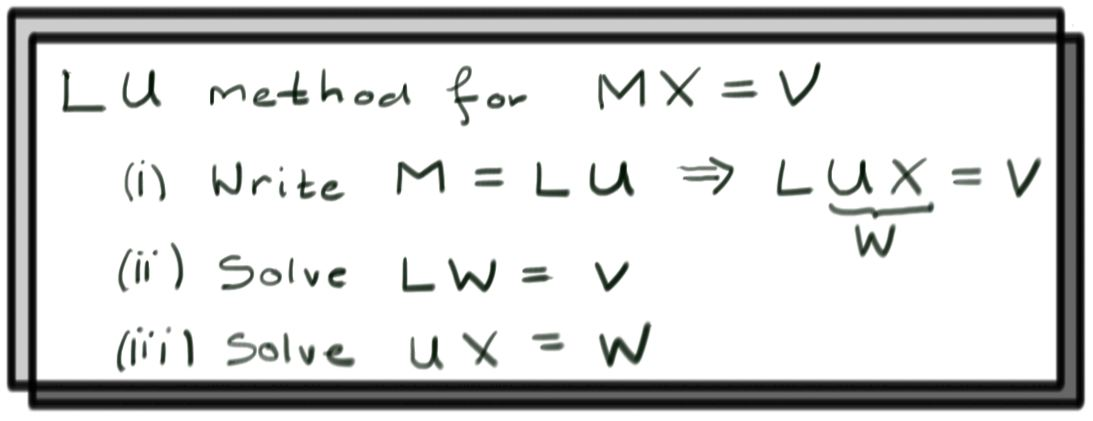
\includegraphics[scale=.3]{\luDecompPath/LU_solution.jpg}
\end{center}
%\end{figure}

\section{Finding an $LU$ Decomposition.}
\label{finding_LU_decomp}
 
For any given matrix, there are actually many different $LU$ decompositions.  However, there is a unique $LU$ decomposition in which the $L$ matrix has ones on the diagonal. In that case $L$ is called a \emph{lower unit triangular matrix}\index{Lower unit triangular matrix}.

To find the $LU$ decomposition, we'll create two sequences of matrices $L_0, L_1, \ldots$ and $U_0, U_1, \ldots$ such that at each step, $L_iU_i=M$.  Each of the $L_i$ will be lower triangular, but only the last $U_i$ will be upper triangular.

Start by setting $L_0=I$ and $U_0=M$, because $L_0U_0=M$. A main concept of this calculation is captured by the following example:

\begin{example}
Consider $$E=\begin{pmatrix}1&0\\\lambda&1\end{pmatrix}\, ,\qquad M=\begin{pmatrix}a&b&c&\cdots\\d&e&f&\cdots\end{pmatrix}\, .$$
Lets compute $EM$
$$
EM=\begin{pmatrix}a&b&c&\cdots\\d+\lambda a&e+\lambda b&f+\lambda c&\cdots\end{pmatrix}\, ,.
$$
Something neat happened here: multiplying $M$ by $E$ performed the row operation $R_2\to R_2+\lambda R-1$ on $M$.
Another interesting fact:
$$
E^{-1}:=\begin{pmatrix}1&0\\-\lambda&1\end{pmatrix}
$$ 
obeys (check this yourself...)
$$
E^{-1} E = 1\, .
$$
Hence $M=E^{-1} E M$ or, writing this out
$$
\begin{pmatrix}a&b&c&\cdots\\d&e&f&\cdots\end{pmatrix}=\begin{pmatrix}1&0\\-\lambda&1\end{pmatrix} \begin{pmatrix}a&b&c&\cdots\\d+\lambda a&e+\lambda b&f+\lambda c&\cdots\end{pmatrix}\, .
$$
Here the matrix on the left is lower triangular, while the matrix on the right has had a row operation performed on it.
\end{example}




\vspace{2mm}
We would like to  use the first row of $U_0$ to zero out the first entry of every row below it.  For our running example, $$U_0=M=\begin{pmatrix}
6 & 18 & 3 \\
2 & 12 & 1 \\
4 & 15 & 3 
\end{pmatrix}\, ,$$ so we would like to perform the row operations $R_2\to R_2 -\frac 13 R_1$ and $R_3\to R_3-\frac 23R_1$.
%so the second row minus $\frac{1}{3}$ of the first row will zero out the first entry in the second row.  Likewise, the third row minus $\frac{2}{3}$ of the first row will zero out the first entry in the third row.
If we perform these row operations on $U_0$ to produce 
$$U_1=\begin{pmatrix}
6 & 18 & 3 \\
0 & 6 & 0 \\
0 & 3 & 1 
\end{pmatrix}\, ,$$
we need to multiply this on the left by a lower triangular matrix $L_1$ so that the product $L_1U_1=M$ still.
The above example shows how to do this:
Set $L_1$ to be the lower triangular matrix whose first column is filled with the minus constants used to zero out the first column of $M$.  Then $$L_1 = \begin{pmatrix}
1 & 0 & 0 \\[1mm]
\frac{1}{3} & 1 & 0 \\[1mm]
\frac{2}{3} & 0 & 1 
\end{pmatrix}\, .$$  
%Set $U_1$ to be the matrix obtained by zeroing out the first column of $M$.  Then $U_1=\begin{pmatrix}
%6 & 18 & 3 \\
%0 & 6 & 0 \\
%0 & 3 & 1 
%\end{pmatrix}$.
By construction $L_1 U_1=M$, but you should compute this yourself as a double check.

Now repeat the process by zeroing the second column of $U_1$ below the diagonal using the second row of $U_1$ using the row operation
$R_3\to R_3-\frac 12 R_2$ to produce
$$U_2=\begin{pmatrix}6&18&3\\0&6&0\\0&0&1\end{pmatrix}\, .$$
The matrix that undoes this row operation is obtained in the same way we found $L_1$ above and is:
$$
\begin{pmatrix}
1&0&0\\
0&1&0\\
0&\frac 12& 0
\end{pmatrix}\, .
$$
Thus our answer for $L_2$ is the product of this matrix with $L_1$, namely
$$
L_2=
\begin{pmatrix}
1 & 0 & 0 \\[1mm]
\frac{1}{3} & 1 & 0 \\[1mm]
\frac{2}{3} & 0 & 1 
\end{pmatrix}\begin{pmatrix}
1&0&0\\
0&1&0\\
0&\frac 12& 0
\end{pmatrix}
=\begin{pmatrix}
1 & 0 & 0 \\[1mm]
\frac{1}{3} & 1 & 0 \\[1mm]
\frac{2}{3} & \frac{1}{2} & 1 
\end{pmatrix}\, .
$$
Notice that it is lower triangular because 

\begin{center}
\textcolor{brown}{THE PRODUCT OF LOWER TRIANGULAR MATRICES IS ALWAYS LOWER TRIANGULAR!}
\end{center}

\noindent
Moreover it is obtained by recording minus the constants used for all our row operations in the appropriate columns (this always works this way).
Moreover, $U_2$ is upper triangular and $M=L_2U_2$, we are done!
Putting this all together we have
$$M=\begin{pmatrix}
6 & 18 & 3 \\
2 & 12 & 1 \\
4 & 15 & 3 
\end{pmatrix}= \begin{pmatrix}
1 & 0 & 0 \\[1mm]
\frac{1}{3} & 1 & 0 \\[1mm]
\frac{2}{3} & \frac{1}{2} & 1 
\end{pmatrix}\begin{pmatrix}
6 & 18 & 3 \\
0 & 6 & 0 \\
0 & 0 & 1 
\end{pmatrix}\, .$$  
%Since $U_2$ is upper-triangular, we're done.  Inserting the new number into $L_1$ to get $L_2$ really is safe: the numbers in the first column don't affect the second column of $U_1$, since the first column of $U_1$ is already zeroed out.

If the matrix you're working with has more than three rows, just continue this process by zeroing out the next column below the diagonal, and repeat until there's nothing left to do.

\videoscriptlink{lu_decomposition_example.mp4}{Another $LU$ decomposition example}{scripts_lu_decomposition_example}

The fractions in the $L$ matrix are admittedly ugly.  For two matrices $LU$, we can multiply one entire column of $L$ by a constant $\lambda$ and divide the corresponding row of $U$ by the same constant without changing the product of the two matrices.  Then:

\begin{eqnarray*}
LU &=& \begin{pmatrix}
1 & 0 & 0 \\[1mm]
\frac{1}{3} & 1 & 0 \\[1mm]
\frac{2}{3} & \frac{1}{2} & 1 
\end{pmatrix}
I
\begin{pmatrix}
6 & 18 & 3 \\
0 & 6 & 0 \\
0 & 0 & 1 
\end{pmatrix} \\
&=&
\begin{pmatrix}
1 & 0 & 0 \\[1mm]
\frac{1}{3} & 1 & 0 \\[1mm]
\frac{2}{3} & \frac{1}{2} & 1 
\end{pmatrix}
\begin{pmatrix}
3 & 0 & 0 \\
0 & 6 & 0 \\
0 & 0 & 1 
\end{pmatrix}
\begin{pmatrix}
\frac{1}{3} & 0 & 0 \\[1mm]
0 & \frac{1}{6} & 0 \\[1mm]
0 & 0 & 1 
\end{pmatrix}
\begin{pmatrix}
6 & 18 & 3 \\
0 & 6 & 0 \\
0 & 0 & 1 
\end{pmatrix} \\
&=&
\begin{pmatrix}
3 & 0 & 0 \\
1 & 6 & 0 \\
2 & 3 & 1 
\end{pmatrix}\begin{pmatrix}
2 & 6 & 1 \\
0 & 1 & 0 \\
0 & 0 & 1 
\end{pmatrix}.
\end{eqnarray*}
The resulting matrix looks nicer, but isn't in standard (lower unit triangular matrix) form.

\reading{11}{2}
%\href{\webworkurl ReadingHomework11/2/}{Reading homework: problem 11.2}

For matrices that are not square, $LU$ decomposition still makes sense.  Given an $m\times n$ matrix $M$, for example we could write $M=LU$ with $L$ a square lower unit triangular matrix, and $U$ a rectangular matrix.  Then $L$ will be an $m\times m$ matrix, and $U$ will be an $m\times n$ matrix (of the same shape as $M$).  From here, the process is exactly the same as for a square matrix.  We create a sequence of matrices $L_i$ and $U_i$ that is eventually the $LU$ decomposition.  Again, we start with $L_0=I$ and $U_0=M$.

\begin{example}
Let's find the $LU$ decomposition of $M=U_0=\begin{pmatrix}
-2 & 1 & 3 \\
-4 & 4 & 1 
\end{pmatrix}$.  Since $M$ is a $2\times 3$ matrix, our decomposition will consist of a $2\times 2$ matrix and a $2\times 3$ matrix.  Then we start with $L_0=I_2=\begin{pmatrix}
1 & 0 \\
0 & 1
\end{pmatrix}$.

The next step is to zero-out the first column of $M$ below the diagonal.  There is only one row to cancel, then, and it can be removed by subtracting $2$ times the first row of $M$ to the second row of $M$.  Then:

\[
L_1=\begin{pmatrix}
1 & 0 \\
2 & 1
\end{pmatrix}, \qquad 
U_1 = \begin{pmatrix}
-2 & 1 & 3 \\
0 & 2 & -5 
\end{pmatrix}
\]
Since $U_1$ is upper triangular, we're done.  With a larger matrix, we would just continue the process.
\end{example}





\section{Block $LDU$ Decomposition}

Let $M$ be a square block matrix with square blocks $X,Y,Z,W$ such that $X^{-1}$ exists.  Then $M$ can be decomposed as a block $LDU$ decomposition, where $D$ is block diagonal, as follows:
\[
M=\begin{pmatrix}
X & Y \\
Z & W
\end{pmatrix}
\]

Then: \[M=\begin{pmatrix}
I &  0 \\
ZX^{-1} & I
\end{pmatrix}\begin{pmatrix}
X & 0 \\
0 & W-ZX^{-1}Y
\end{pmatrix}\begin{pmatrix}
I & X^{-1}Y \\
0 & I
\end{pmatrix}.\]
This can be checked explicitly simply by block-multiplying these three matrices.

\videoscriptlink{lu_decomposition_blocks.mp4}{Block $LDU$ Explanation}{scripts_lu_decomposition_blocks}

\begin{example}
For a $2\times 2$ matrix, we can regard each entry as a block.
\[
\begin{pmatrix}
1 & 2 \\
3 & 4
\end{pmatrix}=
\begin{pmatrix}
1 & 0 \\
3 & 1
\end{pmatrix}
\begin{pmatrix}
1 & 0 \\
0 & -2
\end{pmatrix}
\begin{pmatrix}
1 & 2 \\
0 & 1
\end{pmatrix}
\]
By multiplying the diagonal matrix by the upper triangular matrix, we get the standard $LU$ decomposition of the matrix.
\end{example}


%\section*{References}
%Wikipedia:
%\begin{itemize}
%\item \href{http://en.wikipedia.org/wiki/LU_decomposition}{$LU$ Decomposition}
%\item \href{http://en.wikipedia.org/wiki/Block_LU_decomposition}{Block $LU$ Decomposition}
%\end{itemize}

\section{Review Problems}



\begin{enumerate}

\item Let $D=\begin{pmatrix}
\lambda_1 & \mc0 \\
\mc0 & \lambda_2 \\
\end{pmatrix}$.
\begin{enumerate}
\item Write $D$ in terms of the vectors $e_1$ and $e_2$, and their transposes.
\item Suppose $P=\begin{pmatrix}
a & b \\
c & d \\
\end{pmatrix}$ is invertible.  Show that $D$ is similar to
\[
M=\frac{1}{ad-bc}\begin{pmatrix}
\lambda_1ad-\lambda_2bc & -(\lambda_1-\lambda_2)ab \\[1mm]
(\lambda_1-\lambda_2)cd & -\lambda_1bc + \lambda_2ad
\end{pmatrix}.
\]
\item Suppose the vectors $\rowvec{a,b}$ and $\rowvec{c,d}$ are orthogonal.  What can you say about $M$ in this case? (Hint: think about what \(M^T\) is equal to.)
\end{enumerate}

\phantomnewpage

\item \label{orthogprob} Suppose $S=\{v_1, \ldots, v_n \}$ is an \emph{orthogonal} (not orthonormal) basis for~$\Re^n$.  Then we can write any vector $v$ as $v=\sum_ic^iv_i$ for some constants $c^i$.  Find a formula for the constants $c^i$ in terms of $v$ and the vectors in~$S$.

\Videoscriptlink{orthonormal_bases_hint.mp4}{Hint}{scripts_orthonormal_bases_hint}
\phantomnewpage

\item \label{orthogprojprob} Let $u,v$ be linearly independent vectors in $\Re^3$, and $P=\spa \{ u,v\}$ be the plane spanned by $u$ and $v$.  
\begin{enumerate}
\item Is the vector $v^\bot := v-\frac{u\cdot v}{u\cdot u}u$ in the plane $P$?
\item  What is the (cosine of the) angle between $v^\bot$ and $u$?
\item %Given your solution to the above, 
How can you find a third vector perpendicular to both $u$ and $v^\bot$?
\item  Construct an orthonormal basis for $\Re^3$ from $u$ and $v$.
\item  Test your abstract formul\ae\ starting with 
\[
u=\rowvec{1 , 2 , 0} \text{ and } v=\rowvec{0 , 1 , 1}.
\]
\end{enumerate}

\Videoscriptlink{orthonormal_bases_hint3.mp4}{Hint}{scripts_orthonormal_bases_hint3}

\phantomnewpage



\item Find an orthonormal  basis for $\Re^4$ which includes $(1,1,1,1)$ using the following procedure:\\
\begin{enumerate} 
\item Pick a vector perpendicular to the vector 
$$v_1 =\colvec{1\\1\\1\\1}$$ from the solution set of the matrix equation $$v_1^Tx=0\, .$$ Pick the vector $v_2$ obtained from the standard Gaussian elimination procedure which is the coefficient of $x_2$.
\item Pick a vector perpendicular to both $v_1$ and $v_2$ from the solutions set of the matrix equation $$\colvec{v_1^T\\[1mm]v_2^T}x=0\, .$$ Pick the vector $v_3$ obtained from the standard Gaussian elimination procedure with $x_3$ as the coefficient. 
\item Pick a vector perpendicular to $v_1,v_2,$ and $v_3$ from the solution set of the matrix equation $$\colvec{v_1^T\\[1mm]v_2^T\\[1mm]v_3^T}x=0\, .$$  Pick the vector $v_4$ obtained from the standard Gaussian elimination procedure with $x_3$ as the coefficient. 
\item Normalize the four vectors obtained   above.
\end{enumerate}


\item Use the inner product $$f\cdot g := \int_0^1 f(x)g(x)dx$$  on the vector space $V={\rm span} \{1,x,x^2,x^3\}$ to perform the Gram-Schmidt procedure on the set of vectors $\{1,x,x^2,x^3\}$. 

\item Use the inner product $$f\cdot g := \int_0^{2\pi} f(x)g(x)dx$$  on the vector space $V={\rm span} \{\sin(x),\sin(2x),\sin(3x) \}$ to perform the Gram-Schmidt procedure on the set of vectors $\{\sin(x),\sin(2x),\sin(3x) \}$. \\
Try to build an orthonormal basis for the vector space $$\spa \{ \sin(nx)~| ~n\in \N \}\, .$$
%What do you suspect about the vector space $\spa \{ \sin(nx)~| ~n\in \N \}$?\\
%What do you suspect about the vector space $\spa \{ \sin(ax)~|~ a \in \Re \}$?
\item 
\begin{enumerate}
\item
Show that if $Q$ is an orthogonal $n\times n$ matrix, then $$u\dotprod v = (Qu)\dotprod (Qv)\, ,$$ for any $u,v\in \Re^n$. That is, $Q$ preserves the inner product. 
\item Does $Q$ preserve the outer product? 
\item  If the set of vectors $\{ u_1,\dots,u_n\}$ is orthonormal and $\{ \lambda_1,\cdots,\lambda_n\}$ is a set of numbers, 
then what are the eigenvalues and eigenvectors of the matrix
$M=\sum_{i=1}^n \lambda_i u_i u_i^T$? 
\item How would the eigenvectors and eigenvalues of this matrix change if we replaced  $\{ u_1,\dots,u_n\}$ by $\{ Qu_1,\dots,Q u_n\}$?
\end{enumerate}


\item Carefully write out the Gram-Schmidt procedure for the set of vectors 
$$\left\{ \colvec{1\\1\\1}, \colvec{1\\-1\\1}, \colvec{1\\1\\-1} \right\} \, .$$ Is it possible to rescale the second vector obtained in the procedure to a vector with integer components? 


\item 
\label{basisortho}
\begin{enumerate}
\item Suppose $u$ and $v$ are linearly independent.  Show that $u$ and $v^\perp$ are also linearly independent.  Explain why $\{u, v^\perp\}$ is a basis for $\spa \{u,v\}$.



\Videoscriptlink{gram_schmidt_and_orthogonal_complements_hint.mp4}{Hint}{gram_schmidt_and_orthogonal_complements_hint}

\item Repeat the previous problem, but with three independent vectors $u,v,w$
 where $v^\perp$ and $w^\perp$ are as defined by the Gram-Schmidt procedure. 
\end{enumerate}

\phantomnewpage


\item \label{QRprob} Find the $QR$ factorization of
$$
M=\begin{pmatrix}1&0&\phantom{\!-}2\\-1&2&0\\-1&-2&2
\end{pmatrix}\, .
$$

\phantomnewpage

\item Given any three vectors $u,v,w$, when do $v^\perp$ or $w^\perp$ of the Gram--Schmidt procedure vanish?

\phantomnewpage

\item For $U$ a subspace of $W$, use the subspace theorem to check that $U^\perp$ is a subspace of $W$.

\phantomnewpage


\phantomnewpage

\item %(Extra Credit) 
Let $S_n$ and $A_n$ define the space of $n \times n$ symmetric and anti-symmetric matrices, respectively. These are subspaces of the vector space $M^n_n$ of all $n\times n$ matrices. What is $\dim M^n_n$, $\dim S_n$, and $\dim A_n$? Show that $M^n_n = S_n + A_n$. Define an inner product on square matrices
$$
M\cdot N ={\rm tr} MN\, .
$$
Is $A_n^{\perp}=S_n$? Is $M^n_n = S_n \oplus A_n$?

%\emph{Hint: Note that $\dim S_n = \dim U_n$ where $U_n$ is the vector space of all $n \times n$ upper triangular matrices, and also note that $\dim A_n = \dim \widetilde{U}_n$ where $\widetilde{U}_n$ is the vector space of all strictly $n \times n$ upper triangular matrices (\emph{i.e.} the diagonal entries are all 0).}

\item The vector space $V={\rm span} \{ \sin(t),\sin(2t), \sin(3t) , \sin(3t)\}$ has an inner product: 
$$f\cdot g:=\int _0^{2\pi}f(t)g(t) dt\, .$$ Find the orthogonal compliment to $U={\rm span} \{ \sin(t)+\sin(2t) \}$ in $V$. Express $\sin(t)-\sin(2t)$ as  the sum of vectors from $U$ and $U^\perp$.

\end{enumerate}

\phantomnewpage

\newpage



%\chapter{\gaussElimTitle}

\label{gaussElim}

You have seen that systems of linear equations can be written as matrix equations.
You will see that Gaussian elimination is an efficient \gls{shorthand} for (maximally) simplifying a system of linear equations (or matrix equation).

%You might get the feeling that you are learning to do Gaussian elimination only so that you can tell your computer how too do it in the future. There is more than that going on here. Let us foreshadow chapter 3; as we attempt to streamline the process of elimination we will discover the building blocks of matrices. 



%In \Lecture~\ref{warmup}  we looked performed elimination on a system of equations. 
%It was nice to do this elimination by adding subtracting an multiplying wholes equations at a time. 
%Lets do another example with the system
%\begin{eqnarray}
%	x\ +\ y & = & 27\nn \\
%	2x-\ y & = &\  0\nn \,.
%\end{eqnarray}
%Adding the first equation to the second then dividing by 3 gives
%\begin{eqnarray}
%	x\ +\ 0 & = & 9\nn \\
%	2x-\ y & = &\  0\nn \,.
%\end{eqnarray}
%Subtracting rice the first from the second then dividing by $-1$ gives
%\begin{eqnarray}
%	x \phantom{\ +\ y}& = &\  9\nn \\
%	\phantom{x\ +\ }y & = & 18\, .\nn
%\end{eqnarray}
%
%\noindent
%The maximum number of terms have been eliminated from each equation, and the result is an obvious statement of the solution. 
%\\
%
%We also learned to write such a linear system using a matrix and two vectors. In this case the original linear system can be written
%
%\begin{equation*}
%    \begin{pmatrix}
%      1             &1  \\
%      2             &-1
%    \end{pmatrix}
%  \colvec{x \\ y}
%  =
%  \colvec{27 \\ 0}\, .
%\end{equation*}
%
%
%\noindent
%Likewise, the system of equations that we obtained after elimination can be written
%
%\begin{equation*}
%    \begin{pmatrix}
%      1             &0  \\
%      0             &1
%    \end{pmatrix}
%  \colvec{x \\ y}
%  =
%  \colvec{9 \\ 18} \, .
%\end{equation*}
%\\
%
%%\noindent
%By the way, the matrix $$I=    \begin{pmatrix}
%      1             &0  \\
%      0             &1
%    \end{pmatrix}$$ is called the \emph{Identity Matrix}\index{Identity matrix!$2\times2$}.  She will be very important to us. You should check that if $v$ is any vector, then $$Iv=v\, .$$
%    
%Here is a nice way to summarize your goal when performing the process we are calling elimination elimination; manipulate the system of equations until the resulting system can be written as a matrix equation with the identity matrix.

%%%%%%%%%%%%%%%%%%%%%%%%%%%%%%%%%%
\section{Augmented Matrix Notation for Linear Systems}

%A useful shorthand for a  system of linear equations is an \hypertarget{augmented_matrix}{\emph{Augmented Matrix}}\index{Augmented matrix~$2\times2$}. 
We will introduce this notation through examples: 
The linear system 
\begin{eqnarray}
	x\ +\ y & = & 27\nn \\
	2x-\ y & = &\  0\nn \,
\end{eqnarray}
is denoted by the augmented matrix

\[
\begin{amatrix}{2}
1 &1 &27 \\ 2 &-1 & 0
\end{amatrix}
\]

\noindent
This is truly minimalist notation. It is even more minimal then the matrix notation  
\begin{equation*}
    \begin{pmatrix}
      1             &1  \\
      2             &-1
    \end{pmatrix}
  \colvec{x \\ y}
  =
  \colvec{27 \\ 0}\, .
\end{equation*}
All three of the above equations denote the same thing. 


\videoscriptlink{gaussian_elimination_more_background.mp4}{Augmented Matrix Notation}{script_gaussian_elimination_more}

Going up in size,
the system
\begin{eqnarray*}
1x + 3y + 2z + 0w   =9 \\ 
6x + 2y + 0z   -2w  =0  \\
-1x+ 0 y + 1 z + 1w  =3 
\end{eqnarray*}
is denoted by the augmented matrix
\[
\begin{amatrix}{4}
1 & 3 & 2 & 0  & 9 \\ 
6 & 2 & 0  & -2 & 0  \\
-1& 0  & 1  & 1 & 3
\end{amatrix}
\]
%When writing a system of equations one can write out the terms with zero for coefficients or not
%\begin{eqnarray*}
%1x + 3y + 2z  \phantom{+ 0w}   =9 \\ 
%6x + 2y \phantom{ + 0z}   -2w  =0  \\
%-1x  \phantom{+0 y} + 1 z + 1w  =3 
%\end{eqnarray*}
As a matrix equation the system reads
\begin{eqnarray*}
\left(\begin{array}{cccc}
1 & 3 & 2 & 0   \\ 
6 & 2 & 0  & -2   \\
-1& 0  & 1  & 1 
\end{array}\right)
\colvec{ x\\ y\\z\\w}
=\colvec{ 9\\0\\3}
\end{eqnarray*}




Here's the general case:  The number of equations in the linear system is the number of rows $r$ in the augmented matrix, and the number of columns $k$ in the matrix left of the vertical line is the number of unknowns.
\[
\begin{amatrix}{4}
a^1_1 & a^1_2 & \cdots & a^1_k & b^1 \\ 
a^2_1 & a^2_2 & \cdots & a^2_k & b^2 \\ 
\vdots & \vdots & & \vdots & \vdots  \\
a^r_1 & a^r_2 & \cdots & a^r_k & b^r \\ 
\end{amatrix}
\]
Entries left of the divide carry two indices; subscript denotes column number, superscript denotes row number. We emphasize, the superscripts here do not denote exponents.  

%Aside: most people don't like  indexing by superscripts at first. However, kind of index placement will later facilitate Einstein's summation convention, which Einstein himself described as his greatest contribution to the sciences. 

Make sure you can write out the system of equations and the associated matrix equation for any augmented matrix. 
\reading{2}{1}




We now have three ways or writing the same question. 
Lets put them side by side as we solve the system using a nice algebra trick: we will strategically add and subtract equations.

\begin{example}  (how matrix equations and augmented matrices change in elimination)
\begin{eqnarray*}
   \left.
\begin{array}{lcr}
	x\ +\ y & = & 27 \\
	2x-\ y & = &\  0 
     \end{array}
   \right\} 
   \Leftrightarrow
    \begin{pmatrix}
      1             &1  \\
      2             &-1
    \end{pmatrix}
  \colvec{x \\ y}
  =
  \colvec{27 \\ 0}
  \Leftrightarrow
 \begin{amatrix}{2}
1 &1 &27 \\ 2 &-1 & 0
\end{amatrix}
  \end{eqnarray*}
Let the new first equation be the sum of the first and second equations
\begin{eqnarray*}
   \left.
\begin{array}{lcr}
	3x\ +\ 0 & = & 27 \\
	2x-\ y & = &\  0 
     \end{array}
   \right\} 
   \Leftrightarrow
    \begin{pmatrix}
      3             &0  \\
      2             &-1
    \end{pmatrix}
  \colvec{x \\ y}
  =
  \colvec{27 \\ 0}
  \Leftrightarrow
 \begin{amatrix}{2}
3 &0 &27 \\ 2 &-1 & 0
\end{amatrix}
  \end{eqnarray*}
Let the new first equation be the old first equation divided by 3
 \begin{eqnarray*}
   \left.
\begin{array}{lcr}
	x\ +\ 0 & = & 9 \\
	2x-\ y & = &\  0 
     \end{array}
   \right\} 
   \Leftrightarrow
    \begin{pmatrix}
      1             &0  \\
      2             &-1
    \end{pmatrix}
  \colvec{x \\ y}
  =
  \colvec{9 \\ 0}
  \Leftrightarrow
 \begin{amatrix}{2}
1 &0 &9 \\ 2 &-1 & 0
\end{amatrix}
  \end{eqnarray*}
Let the new second equation be the old second equation minus two times the first equation 
\begin{eqnarray*}
   \left.
\begin{array}{lcr}
	x\ +\ 0 & = & 9 \\
	0-\ y & = &\  -18
     \end{array}
   \right\} 
   \Leftrightarrow
    \begin{pmatrix}
      1             &0  \\
      0             &-1
    \end{pmatrix}
  \colvec{x \\ y}
  =
  \colvec{9 \\ -18}
  \Leftrightarrow
 \begin{amatrix}{2}
1 &0 &9 \\ 0 &-1 & -18
\end{amatrix}
  \end{eqnarray*}
Let the new  second equation be the old second equation divided by -1
\begin{eqnarray*}
   \left.
\begin{array}{lcr}
	x + 0 & = & \ 9 \\
	0 + y & = &  18
     \end{array}
   \right\} 
   \Leftrightarrow
    \begin{pmatrix}
      1             &0  \\
      0             &1
    \end{pmatrix}
  \colvec{x \\ y}
  =
  \colvec{9 \\ 18}
  \Leftrightarrow
 \begin{amatrix}{2}
1 &0 &9 \\ 0 &1 & 18
\end{amatrix}
  \end{eqnarray*}
\end{example}
Did you see what the strategy was? To eliminate $y$ from the first question and then eliminate $x$ from the second. The result was a plain statement of the solution. But the quantity of writing here was atrocious. 

Here is the big idea: 
Everywhere in the the instructions we can replace the word ``equation" with the word ``row" and interpret the instructions as telling us what to do with the augmented matrix instead of the system of equations.
The result is a process called {\it Gaussian elimination}\index{Gaussian elimination}: 
%
%\begin{example} of Gaussian elimination
%\begin{eqnarray*}
% \begin{amatrix}{2}
%1 &1 &27 \\ 2 &-1 & 0
%\end{amatrix}
%  \end{eqnarray*}
%Let the new first row be the sum of the first and second rows
%\begin{eqnarray*}
% \begin{amatrix}{2}
%3 &0 &27 \\ 2 &-1 & 0
%\end{amatrix}
%  \end{eqnarray*}
%Let the new first row be the old first row divided by 3
% \begin{eqnarray*}
% \begin{amatrix}{2}
%1 &0 &9 \\ 2 &-1 & 0
%\end{amatrix}
%  \end{eqnarray*}
%Let the new second row be the old second row minus two times the first row 
%\begin{eqnarray*}
% \begin{amatrix}{2}
%1 &0 &9 \\ 0 &-1 & -18
%\end{amatrix}
%  \end{eqnarray*}
%Let the new  second row be the old second row divided by -1
%\begin{eqnarray*}
% \begin{amatrix}{2}
%1 &0 &9 \\ 0 &1 & 18
%\end{amatrix}
%  \end{eqnarray*}
%The solution can be read off very quickly, and the notation was very minimal. 
%\end{example}
% At each step, the augmented matrices encode systems of equations which have the same solutions. Lets make this idea more formal, and introduce some notation to convey the idea.
%

%%%%%%%%%%%%%%%%%%%%%%%%%%%%%%%%%%%%
%%%%%%%%%%%%%%%%%%%%%%%%%%%%%%%%%%%%

\section{Equivalence and the Act of Solving}


%Two augmented matrices corresponding to linear systems 
%%{\it that actually have solutions} %cmon, this idea has not even been introduced
%are said to be \hypertarget{roweq}(row) 
%\emph{equivalent}\index{Row equivalence} if they have the \emph{same} solutions.
%To denote this 

We introduce the symbol $\sim$ which is called ``tilde" but should be read as  ``is equivalent to''. For example we found above that
\[
\begin{amatrix}{2}
1 &1 &27 \\ 2 &-1 &0
\end{amatrix}
\sim
\begin{amatrix}{2}
1 &0 &9 \\ 2 &-1 & 0
\end{amatrix}
\sim
\begin{amatrix}{2}
1 & 0&9 \\   0& 1 & 18
\end{amatrix}
\]
and certainly the last of these is our favorite!
\videoscriptlink{gaussian_elimination_background.mp4}{Equivalence Example}{script_gaussian_elimination_background}

%\videoscriptlink{gaussian_elimination_3_3_example.mp4}{A $3 \times 3$ example}{scripts_gaussian_elimination_3_3_example}

Setting up a string of equivalences like this is a means of solving a system of linear equations. This is the main idea of chapter 2.

\begin{example} (Using Gaussian elimination to solve a system of linear equations)
\begin{eqnarray*}
   \left.
\begin{array}{lcr}
	x +\ y & = & 5 \\
	x + 2y & = &\  8
     \end{array}
   \right\} 
   \Leftrightarrow
\begin{amatrix}{2}
1 &1 &5 \\ 1 &2 & 8
\end{amatrix}
\sim
\begin{amatrix}{2}
1 &1 &5 \\ 0 &1 & 3
\end{amatrix}
\sim
\begin{amatrix}{2}
1 &0 &2 \\ 0 &1 & 3
\end{amatrix}
\Leftrightarrow
\left\{
\begin{array}{lcr}
	x + 0 & = & 2 \\
	 0 + y & = &\  3
     \end{array}
   \right.
\end{eqnarray*}  
Note that we used the top left $1$ to make the bottom left entry zero. For this reason we call that number a pivot; imagine a wiper blade hanging down form the top left slot wiping the lower left slot away. Similarly the bottom right slot was used to wipe away the top right slot, so it is called a pivot. 
\end{example}

This {\it pivot} jargon is helpful for describing the goings on in Gaussian elimination. Be sure you understand the idea before moving on. 

%%%%%%%%%%%%%%%%%%%%%%%%%%%%%%%%%%%

\section{Reduced Row Echelon Form}
For a system of two linear  equations, the goal in Gaussian elimination is to have the part of the augmented matrix left of the dividing line become the matrix
 $$I=    \begin{pmatrix}
      1             &0  \\
      0             &1
    \end{pmatrix}$$ 
called the \emph{Identity Matrix}\index{Identity matrix!$2\times2$}, since this would give the simple statement of a solution $x=a,y=b$. The situation is similar for larger systems of equations.
\reading{2}{2} %a 3x3 example with one solution>



\noindent
This can't always be done.

\begin{example} (Redundant equations)
 \begin{eqnarray*}
   \left.
\begin{array}{lcr}
	\ x + \ y & = & 2 \\
	2x + 2y & = &  4
     \end{array}
   \right\} 
   \Leftrightarrow
\begin{amatrix}{2}
1 &1 &2 \\ 2 &2 & 4
\end{amatrix}
\sim
\begin{amatrix}{2}
1 &1 &2 \\ 0 &0 & 0
\end{amatrix}
%\sim
%\begin{amatrix}{2}
%1 &0 &2 \\ 0 &1 & 3
%\end{amatrix}
\Leftrightarrow
\left\{
\begin{array}{lcr}
	x + y & = & 2 \\
	 0 + 0 & = &  0
     \end{array}
   \right.
\end{eqnarray*}  
This example demonstrates if one equation is a multiple of the other the identity matrix can not be a reached. This is because the first step in elimination will make the second row a row of zeros. Notice that solutions still exists $x=1,y=1$ is a solution. The last augmented matrix here is in RREF.
\end{example}

\begin{example} (Inconsistent equations)
 \begin{eqnarray*}
   \left.
\begin{array}{lcr}
	\ x + \ y & = & 2 \\
	2x + 2y & = &  5
     \end{array}
   \right\} 
   \Leftrightarrow
\begin{amatrix}{2}
1 &1 &2 \\ 2 &2 & 5
\end{amatrix}
\sim
\begin{amatrix}{2}
1 &1 &2 \\ 0 &0 & 1
\end{amatrix}
%\sim
%\begin{amatrix}{2}
%1 &0 &2 \\ 0 &1 & 3
%\end{amatrix}
\Leftrightarrow
\left\{
\begin{array}{lcr}
	x + y & = & 2 \\
	 0 + 0 & = &  1
     \end{array}
   \right.
\end{eqnarray*}  
This system of equation has a solution if there exists two numbers $x$, and $y$ such that $0+0=1$. That is a tricky way of saying there are no solutions. The last form of the augmented matrix here is in RREF.
\end{example}


\begin{example} (Silly order of equations)\\
A robot might make the following mistake
 \begin{eqnarray*}
   \left.
\begin{array}{lcr}
	0x +  \ y & = & -2 \\
	\ x + y & = &  7
     \end{array}
   \right\} 
   \Leftrightarrow 
\begin{amatrix}{2}
0 &1 & -2\\ 1 &1 & 7
\end{amatrix}
\sim \cdots
\end{eqnarray*}  
and then give up because the the upper left slot can not function as a pivot since the 0 that lives there can not be used to eliminate the zero below it. Of course, the right thing to do is to change the order of the equations before starting
 \begin{eqnarray*}
   \left.
\begin{array}{lcr}
	\ x + y & = &  7
	\\
	0x +  \ y & = & -2 
	     \end{array}
   \right\} 
   \Leftrightarrow
\begin{amatrix}{2}
1 &1 & 7\\ 0 &1 & -2
\end{amatrix}
\sim 
\begin{amatrix}{2}
1 &0 & 9\\ 0 &1 & -2
\end{amatrix}
\Leftrightarrow
\left\{
\begin{array}{lcr}
	x + 0 & = & 9 \\
	 0 + y & = & -2
     \end{array}
   \right.
\end{eqnarray*}  
The third appearance of an augmented matrix here is RREF of the first, and second. That is to say, you can swap rows on your way to RREF.
\end{example}



For larger systems of matrices, these three kinds of problems are the obstruction to obtaining the identity matrix, and hence to a simple statement of a solution in the form $x=a,y=b,...$. 
What can we do to maximally simplify a system of equations in general?
We can do three things corresponding to exchanging the order of equations, multiplying one equation by a constant or adding equations:
\begin{itemize}
\item (Row Swap) Exchange any two rows.
\item (Scalar Multiplication) Multiply any row by a non-zero constant.
\item (Row Sum) Add a multiple of one row to another row.
\end{itemize}
These are called the \emph{Elementary Row Operations}\index{EROs}, or EROs for short. They are the  subject of the next lecture. 
They can be used to achieve \emph{Reduced Row Echelon Form}\index{Reduced row echelon form} (RREF), the maximally simplified augmented matrix, which typically looks like 
\[
\begin{amatrix}{7}
1       	& * & 0		& * & 0		& \cdots& 0		& b^1 \\ 
0	        & 0 & 1		& * & 0		& \cdots& 0		& b^2 \\
0		& 0& 0		& 0 & 1		& \cdots& 0		& b^3 \\  
\vdots  	& \vdots& \vdots	&   & \vdots	& 	& 0			& \vdots \\  
		& &			&  &			&      & 1			& b^k \\  
0		& 0 & 0		& 0 & 0		& \cdots& 0 		& b^{k+1} \\ 
\vdots  	& \vdots & \vdots	&  \vdots & \vdots	& 	& \vdots		& \vdots \\  
0		&  0 & 0		& 0 & 0		& \cdots& 0		& b^r \\ 
\end{amatrix}
\]

%The first non-zero entry in each row is called the \emph{pivot}\index{Pivot}.    
\noindent
The asterisks denote the possibility of arbitrary numbers. (For e.g. 1 in the redundant equations example.)  
If any of the numbers $b^{k+1},\dots b^r$ are non-zero then the system of equations is inconsistent and has no solutions. 


It is essential to be able to visualize how 
RREF can be obtained using (only) elementary row operations in the most general case:
\begin{itemize}
\item Make the leftmost nonzero entry in the top row 1 by multiplication.  
\item Then use that 1 as a pivot to eliminate everything below it. 
\item Then go to the next row and make the leftmost non zero entry 1. 
\item Then use that 1 as a pivot to eliminate everything below {\it and above it}! 
\item Then go to the next row and make the leftmost nonzero entry 1... etc
\end{itemize}
Note that this is not the only way to get to RREF. You might, for example, begin by eliminating everything below the top left entry before setting it to one. 

\videoscriptlink{gaussian_elimination_Beginner_Elimination.mp4}{Beginner Elimination}{script_gaussian_elimination_more}

\noindent
The following properties fully describe  RREF.

\begin{enumerate}
\item  In every row  the left most non-zero entry is  $1$ (and is called a pivot).

\item The pivot of any given row is always to the right of the pivot of the row above it.

\item The pivot is the only non-zero entry in its column.
\end{enumerate}

\begin{example} (Augmented matrix in RREF)
$$
\begin{amatrix}{3} 
1 & 0 & 7 & 0 \\ 
0 & 1 & 3 & 0 \\
0 & 0 & 0 & 1 \\
0 & 0 & 0 & 0 \\
\end{amatrix}
$$
\end{example}

\begin{example} (Augmented matrix NOT in RREF)
$$
\begin{amatrix}{3} 
1 & 0 & 3 & 0 \\ 
0 & 0 & 2 & 0 \\
0 & 1 & 0 & 1 \\
0 & 0 & 0 & 1 \\
\end{amatrix}
$$
Actually, this NON-example breaks all three of the rules!
\end{example}


The reason we need the asterisks in the general form of RREF:
it is not necessary for every column to have a pivot as demonstrated in the ``augmented matrix in RREF" and ``redundant equations" examples above. 
Actually, in full generality where we have asterisks one can have multiple columns with no pivot as one would have in the following

\begin{example} (Consecutive  columns with no pivot in RREF)
 \begin{eqnarray*}
   \left.
\begin{array}{lcr}
	\ x \ + \ y + \ z +  0w & = & 2 \\
	2x + 2y +2z+2w & = &  4
     \end{array}
   \right\} 
   \Leftrightarrow
\begin{amatrix}{4}
1 &1 &1 & 0 &2 \\ 
2 &2 &2 & 1 & 4
\end{amatrix}
\\
\sim
\begin{amatrix}{4}
1 &1 &1 & 0 &2 \\ 
0 &0 &0 & 1 & 0
\end{amatrix}
\Leftrightarrow
\left\{
\begin{array}{lcr}
	x + y +z& = & 2 \\
	 w & = &  0
     \end{array}
   \right.
\end{eqnarray*}  
Note that there was no hope of reaching the identity matrix just because of the shape of the augmented matrix we started with. 
\end{example}


\videoscriptlink{gaussian_elimination_Advanced_Elimination.mp4}{Advanced Elimination}{script_gaussian_elimination_more}



\section{Solution Sets}
%While RREF is not always pretty, it is certainly useful. 
%Our goal  is to solve systems of linear equations. 
RREF represents a maximally simplified version of the original system of equations in the following sense: 
\begin{itemize}
\item As many coefficient of the variables have been set to zero as is possible 
\item As many coefficients of variables have been set to 1 as possible.
\end{itemize}
It is easier to read off solutions from the maximally simplified equations than from the original equations, even when there are infinitely many solutions.

\begin{example}
 \begin{eqnarray*}
\left.
\begin{array}{lcr}
	x  +y    \phantom{+ z}  + 5w & ~  = 1 \\
	\phantom {x+}  \ y  \phantom{+z}   + 2 w & = 6 \\
	\phantom{x+y+} z+         4w & = 8
\end{array}
 \right\}
 \Leftrightarrow
 \begin{amatrix}{4} 
1 & 1 & 0 & 5 & 1 \\ 
0 & 1 & 0 & 2 & 6 \\
0 & 0 & 1 & 4 & 8 
\end{amatrix}
\sim
 \begin{amatrix}{4} 
1 & 0 & 0 & 3 & -5 \\ 
0 & 1 & 0 & 2 & 6 \\
0 & 0 & 1 & 4 & 8 
\end{amatrix}
\\
\Leftrightarrow
\left\{
\begin{array}{lcr}
	x \phantom{+y    + z}  + 3w & ~ \ = -5 \\
	\phantom {x+}   y \, \phantom{+z}  \ + 2 w & = 6 \\
	\phantom{x+y+} z+         4w & = 8
     \end{array}
     \right.
\end{eqnarray*}
In this case, we say that $x,y$, and $z$ are {\it pivot variables}\index{pivot variables} because they appear with pivots as coefficients. Since $w$ never appears with a pivot as a coefficient, 
we say that it is not a pivot variable. %We call it a free variable. 
One way to express the solutions to this system of equations is to put all the pivot variables on one side and all the {\it non-pivot variables}\index{non-pivot variables} on the other side. It is also nice to add the ``freebee equation" $w=w$ to obtain the system
\begin{eqnarray*}
\left.
\begin{array}{lcr}
	x & = -5 -3w \\
	 y  & = 6 -2w\\
	 z & = 8-4w \\
	w & =\phantom{8-4}w          
     \end{array}
     \right\}
     \Leftrightarrow
\colvec{x\\y\\z\\w} = \colvec{-5\\6\\8\\0} + w\colvec{-3\\-2\\-4\\1}
\end{eqnarray*}
where we have written the solution to the corresponding matrix problem. There are infinitely many solutions, one for each value of $z$. We call the collection of all solutions {\it the solution set}\index{solution set}\index{solution set} It is easy to check that the solution corresponding to $w=0$ really does fit into the matrix equation. 
\end{example}


The last example demonstrated the \hypertarget{standard approach}{{\it standard approach}} to solving a system of linear equations in its entirety: write the augmented matrix, obtain RREF, return to the system of equations, and express the non-pivot variables in terms of the pivot variables. 
There are always exactly enough non-pivot variables to index your solutions. 
In any approach, the variables which are not expressed in terms of the other variables are called the {\it free variables}\index{free variables}. The standard approach is to use the non-pivot variables as free variables.

%vid for this?! 
Non-standard approach: solve for $w$ in terms of $z$ and substitute into the other equations. You now have an expression for each component in terms of $z$. But why pick $z$ instead of $y$ or $x$? (or $x+y$?) The standard approach feels natural, and that is why it became the standard.

When you see a RREF augmented matrix with two columns that have no pivot, you know there will be two free variables. 

\begin{example}
 \begin{eqnarray*}
 \begin{amatrix}{4} 
1 & 0 & 7 & 0 & 4 \\ 
0 & 1 & 3 & 4 & 1 \\ 
0 & 0 & 0 & 0 & 0 \\ 
0 & 0 & 0 & 0 & 0 \\ 
\end{amatrix}
\Leftrightarrow
\left\{
\begin{array}{lcr}
	x \phantom{+y}    + 7z  \phantom{+w} & = 4 \\
	\phantom {x+}   y + 3z  {+4w} & = 1 \\
	%\phantom{x+y+z+}          w & = 2
     \end{array}
     \right.
\end{eqnarray*}  
Expressing the pivot variables in terms of the non-pivot variables, and using two freebee equations gives
\begin{eqnarray*}
\left.
\begin{array}{lcr}
	x & = 4 -7z \\
	 y  & = 1 -3z-4w\\
	 z         & = z\\
	w & =w          
     \end{array}
     \right\}
     \Leftrightarrow
\colvec{x\\y\\z\\w} = \colvec{4\\1\\0\\0} + z\colvec{-7\\-3\\1\\0} + w\colvec{0\\-4\\0\\1}
\end{eqnarray*}
There are infinitely many solutions. One solution for each pair of numbers $z,w$. 
\end{example}
You can imagine having three, four, or fifty-six non-pivot columns and the same number of free variables indexing your solutions set. You need to become very adept at reading off solutions of linear systems from the RREF
of their augmented matrix. 

\videoscriptlink{solution_sets_for_systems_example.mp4}{Solution set in set notation}{solution_sets_for_systems_of_linear_equations_example}

\videoscriptlink{elementary_row_operations_worked_examples.mp4}{\hspace{-8mm}Worked examples of Gaussian elimination\hspace{-8mm}}{scripts_elementary_row_operations_worked_examples}


%This example emphasizes different aspects.
%\begin{example}
%$$
%\begin{amatrix}{5} 
%1 & 1 & 0 & 1 & 0 & 1\\ 
%0 & 0 & 1 & 2 & 0 & 2\\ 
%0 & 0 & 0 & 0 & 1 & 3\\ 
%0 & 0 & 0 & 0 & 0 & 0
%\end{amatrix}\, .
%$$
%Here we were not told the names of the variables, so lets just call them $x_1,x_2,x_3,x_4,x_5$.
%(There are always as many of these as there are columns in the matrix before the vertical line; the number of rows,
%on the other hand is the number of linear equations.)
%
%To begin with we immediately notice that there are no pivots in the second and fourth columns so, as per the standard approach, we will be all variables in terms of $x_2$ and $x_4$. 
%Next we see from the second last row that $x_5=3$. The second row says 
%$x_3=2-2x_4=2-2 x_2$.
%The top row then gives $x_1=1-x_2-x_4=1-x_1-x_2$. Again we can write this solution as a vector
%$$
%\colvec{1\\0\\2\\0\\3}+x_1\colvec{-1\\1\\0\\0\\0}+x_2\colvec{-1\\0\\-2\\1\\0}\, .
%$$
%Observe, that since no variables were given at the beginning, we can use any symbols instead of $x_1$ and $x_2$. For example lower case greek letter lambda:
%$$
%\colvec{1\\0\\2\\0\\3}+\lambda_1\colvec{-1\\1\\0\\0\\0}+\lambda_2\colvec{-1\\0\\-2\\1\\0}\, .
%$$
%As a challenge, look carefully at this solution and make sure you can see how every part of it comes from
%the original augmented matrix without every having to reintroduce variables and equations.
%\end{example}
%
%




%\begin{theorem}
%Every augmented matrix is row-equivalent to a \emph{unique} augmented matrix in reduced row echelon form.
%\end{theorem}
%
%\noindent
%In \Lecture~\ref{elemRowOpsPath}, we will see why this is true.

%\section*{Uniqueness of RREF}
%
%\begin{theorem}\label{GJEunique} Gauss-Jordan Elimination produces a unique augmented matrix in RREF.
%\end{theorem}
%
%\begin{proof}
%Suppose Alice and Bob compute the RREF for a linear system but get different results, $A$ and $B$.  Working from the left, discard all columns except for the pivots and the first column in which $A$ and $B$ differ.  By \hyperref[colremove]{Review Problem~\ref{colremove}}, removing columns does not affect row equivalence.  Call the new, smaller, matrices $\hat{A}$ and $\hat{B}$.  The new matrices should look this: $$\hat{A}=\begin{amatrix}{1}
%I_N & a\\
%0 & 0
%\end{amatrix} \mbox{ and } \hat{B}=\begin{amatrix}{1}
%I_N & b\\
%0 & 0
%\end{amatrix}\, ,$$ where $I_N$ is an $N\times N$ identity matrix and $a$ and $b$ are vectors.
%
%Now if $\hat{A}$ and $\hat{B}$ have the same solution, then we must have $a=b$.  But this is a contradiction!  Then $A=B$.
%\end{proof}
%
%\videoscriptlink{elementary_row_operations_proof.mp4}{Explanation of the proof}{scripts_elementary_row_operations_proof}


%\References{
%Hefferon, Chapter One, Section 1
%\\
%Beezer, Chapter SLE, Section RREF
%\\
%Wikipedia, \href{http://en.wikipedia.org/wiki/Row_echelon_form}{Row Echelon Form}}

%\newpage

\section{Review Problems}




\begin{enumerate}

\item Let $D=\begin{pmatrix}
\lambda_1 & \mc0 \\
\mc0 & \lambda_2 \\
\end{pmatrix}$.
\begin{enumerate}
\item Write $D$ in terms of the vectors $e_1$ and $e_2$, and their transposes.
\item Suppose $P=\begin{pmatrix}
a & b \\
c & d \\
\end{pmatrix}$ is invertible.  Show that $D$ is similar to
\[
M=\frac{1}{ad-bc}\begin{pmatrix}
\lambda_1ad-\lambda_2bc & -(\lambda_1-\lambda_2)ab \\[1mm]
(\lambda_1-\lambda_2)cd & -\lambda_1bc + \lambda_2ad
\end{pmatrix}.
\]
\item Suppose the vectors $\rowvec{a,b}$ and $\rowvec{c,d}$ are orthogonal.  What can you say about $M$ in this case? (Hint: think about what \(M^T\) is equal to.)
\end{enumerate}

\phantomnewpage

\item \label{orthogprob} Suppose $S=\{v_1, \ldots, v_n \}$ is an \emph{orthogonal} (not orthonormal) basis for~$\Re^n$.  Then we can write any vector $v$ as $v=\sum_ic^iv_i$ for some constants $c^i$.  Find a formula for the constants $c^i$ in terms of $v$ and the vectors in~$S$.

\Videoscriptlink{orthonormal_bases_hint.mp4}{Hint}{scripts_orthonormal_bases_hint}
\phantomnewpage

\item \label{orthogprojprob} Let $u,v$ be linearly independent vectors in $\Re^3$, and $P=\spa \{ u,v\}$ be the plane spanned by $u$ and $v$.  
\begin{enumerate}
\item Is the vector $v^\bot := v-\frac{u\cdot v}{u\cdot u}u$ in the plane $P$?
\item  What is the (cosine of the) angle between $v^\bot$ and $u$?
\item %Given your solution to the above, 
How can you find a third vector perpendicular to both $u$ and $v^\bot$?
\item  Construct an orthonormal basis for $\Re^3$ from $u$ and $v$.
\item  Test your abstract formul\ae\ starting with 
\[
u=\rowvec{1 , 2 , 0} \text{ and } v=\rowvec{0 , 1 , 1}.
\]
\end{enumerate}

\Videoscriptlink{orthonormal_bases_hint3.mp4}{Hint}{scripts_orthonormal_bases_hint3}

\phantomnewpage



\item Find an orthonormal  basis for $\Re^4$ which includes $(1,1,1,1)$ using the following procedure:\\
\begin{enumerate} 
\item Pick a vector perpendicular to the vector 
$$v_1 =\colvec{1\\1\\1\\1}$$ from the solution set of the matrix equation $$v_1^Tx=0\, .$$ Pick the vector $v_2$ obtained from the standard Gaussian elimination procedure which is the coefficient of $x_2$.
\item Pick a vector perpendicular to both $v_1$ and $v_2$ from the solutions set of the matrix equation $$\colvec{v_1^T\\[1mm]v_2^T}x=0\, .$$ Pick the vector $v_3$ obtained from the standard Gaussian elimination procedure with $x_3$ as the coefficient. 
\item Pick a vector perpendicular to $v_1,v_2,$ and $v_3$ from the solution set of the matrix equation $$\colvec{v_1^T\\[1mm]v_2^T\\[1mm]v_3^T}x=0\, .$$  Pick the vector $v_4$ obtained from the standard Gaussian elimination procedure with $x_3$ as the coefficient. 
\item Normalize the four vectors obtained   above.
\end{enumerate}


\item Use the inner product $$f\cdot g := \int_0^1 f(x)g(x)dx$$  on the vector space $V={\rm span} \{1,x,x^2,x^3\}$ to perform the Gram-Schmidt procedure on the set of vectors $\{1,x,x^2,x^3\}$. 

\item Use the inner product $$f\cdot g := \int_0^{2\pi} f(x)g(x)dx$$  on the vector space $V={\rm span} \{\sin(x),\sin(2x),\sin(3x) \}$ to perform the Gram-Schmidt procedure on the set of vectors $\{\sin(x),\sin(2x),\sin(3x) \}$. \\
Try to build an orthonormal basis for the vector space $$\spa \{ \sin(nx)~| ~n\in \N \}\, .$$
%What do you suspect about the vector space $\spa \{ \sin(nx)~| ~n\in \N \}$?\\
%What do you suspect about the vector space $\spa \{ \sin(ax)~|~ a \in \Re \}$?
\item 
\begin{enumerate}
\item
Show that if $Q$ is an orthogonal $n\times n$ matrix, then $$u\dotprod v = (Qu)\dotprod (Qv)\, ,$$ for any $u,v\in \Re^n$. That is, $Q$ preserves the inner product. 
\item Does $Q$ preserve the outer product? 
\item  If the set of vectors $\{ u_1,\dots,u_n\}$ is orthonormal and $\{ \lambda_1,\cdots,\lambda_n\}$ is a set of numbers, 
then what are the eigenvalues and eigenvectors of the matrix
$M=\sum_{i=1}^n \lambda_i u_i u_i^T$? 
\item How would the eigenvectors and eigenvalues of this matrix change if we replaced  $\{ u_1,\dots,u_n\}$ by $\{ Qu_1,\dots,Q u_n\}$?
\end{enumerate}


\item Carefully write out the Gram-Schmidt procedure for the set of vectors 
$$\left\{ \colvec{1\\1\\1}, \colvec{1\\-1\\1}, \colvec{1\\1\\-1} \right\} \, .$$ Is it possible to rescale the second vector obtained in the procedure to a vector with integer components? 


\item 
\label{basisortho}
\begin{enumerate}
\item Suppose $u$ and $v$ are linearly independent.  Show that $u$ and $v^\perp$ are also linearly independent.  Explain why $\{u, v^\perp\}$ is a basis for $\spa \{u,v\}$.



\Videoscriptlink{gram_schmidt_and_orthogonal_complements_hint.mp4}{Hint}{gram_schmidt_and_orthogonal_complements_hint}

\item Repeat the previous problem, but with three independent vectors $u,v,w$
 where $v^\perp$ and $w^\perp$ are as defined by the Gram-Schmidt procedure. 
\end{enumerate}

\phantomnewpage


\item \label{QRprob} Find the $QR$ factorization of
$$
M=\begin{pmatrix}1&0&\phantom{\!-}2\\-1&2&0\\-1&-2&2
\end{pmatrix}\, .
$$

\phantomnewpage

\item Given any three vectors $u,v,w$, when do $v^\perp$ or $w^\perp$ of the Gram--Schmidt procedure vanish?

\phantomnewpage

\item For $U$ a subspace of $W$, use the subspace theorem to check that $U^\perp$ is a subspace of $W$.

\phantomnewpage


\phantomnewpage

\item %(Extra Credit) 
Let $S_n$ and $A_n$ define the space of $n \times n$ symmetric and anti-symmetric matrices, respectively. These are subspaces of the vector space $M^n_n$ of all $n\times n$ matrices. What is $\dim M^n_n$, $\dim S_n$, and $\dim A_n$? Show that $M^n_n = S_n + A_n$. Define an inner product on square matrices
$$
M\cdot N ={\rm tr} MN\, .
$$
Is $A_n^{\perp}=S_n$? Is $M^n_n = S_n \oplus A_n$?

%\emph{Hint: Note that $\dim S_n = \dim U_n$ where $U_n$ is the vector space of all $n \times n$ upper triangular matrices, and also note that $\dim A_n = \dim \widetilde{U}_n$ where $\widetilde{U}_n$ is the vector space of all strictly $n \times n$ upper triangular matrices (\emph{i.e.} the diagonal entries are all 0).}

\item The vector space $V={\rm span} \{ \sin(t),\sin(2t), \sin(3t) , \sin(3t)\}$ has an inner product: 
$$f\cdot g:=\int _0^{2\pi}f(t)g(t) dt\, .$$ Find the orthogonal compliment to $U={\rm span} \{ \sin(t)+\sin(2t) \}$ in $V$. Express $\sin(t)-\sin(2t)$ as  the sum of vectors from $U$ and $U^\perp$.

\end{enumerate}

\phantomnewpage

\newpage


%New version with EROS and solution sets all in CH2
\chapter{\luDecompTitle}
\label{LUdecomp}

Certain matrices are easier to work with than others.  In this section, we will see how to write any square\footnote{The case where $M$ is not square is dealt with at the end of the lecture.} matrix $M$ as the product of two simpler matrices.  We will write $$M=LU\, ,$$ where:
\begin{itemize}
\item $L$ is \emph{lower triangular}\index{Lower triangular matrix}.  This means that all entries above the main diagonal are zero.  In notation,
$L=(l^i_j)$ with $l^i_j=0$ for all $j>i$.
\[L=\begin{pmatrix}
l^1_1 & 0 & 0 & \cdots \\
l^2_1 & l^2_2 & 0 & \cdots \\
l^3_1 & l^3_2 & l^3_3 & \cdots \\
\vdots & \vdots & \vdots & \ddots \\
\end{pmatrix}
\]

\item $U$ is \emph{upper triangular}\index{Upper triangular matrix}.  This means that all entries below the main diagonal are zero.  In notation,
$U=(u^i_j)$ with $u^i_j=0$ for all $j<i$.
\[U=\begin{pmatrix}
u^1_1 & u^1_2 & u^1_3 & \cdots \\
0 & u^2_2 & u^2_3 & \cdots \\
0 & 0 & u^3_3 & \cdots \\
\vdots & \vdots & \vdots & \ddots \\
\end{pmatrix}
\]
\end{itemize}
$M=LU$ is called an \emph{$LU$ decomposition}\index{LU@$LU$ decomposition} of $M$.

This is a useful trick for  computational reasons; it is much easier to compute the inverse of an upper or lower triangular matrix than general matrices.  Since inverses are useful for solving linear systems, this makes solving any linear system associated to the matrix much faster as well.  The determinant---a very important quantity associated with any square matrix---is very easy to compute for triangular matrices.

\begin{example}
Linear systems associated to upper triangular matrices are very easy to solve by back substitution.
\[
\begin{amatrix}{2}
a & b & 1 \\
0 & c & e \\
\end{amatrix} \ \Rightarrow \ y=\frac{e}{c}\, , \quad x=\frac{1}{a}\left(1-\frac{be}{c}\right)
\]

\[
\begin{amatrix}{3}
1 & 0 & 0 & d \\
a & 1 & 0 & e \\
b & c & 1 & f \\
\end{amatrix} \Rightarrow x=d\, , \qquad y=e-ad\, , \qquad z=f-bd-c(e-ad)
\]
For lower triangular matrices, \emph{back} substitution\index{Back substitution} gives a quick solution; for upper triangular matrices, \emph{forward} substitution\index{Forward substitution} gives the solution.
\end{example}





\section{Using $LU$ Decomposition to Solve Linear Systems}

Suppose we have $M=LU$ and want to solve the system
\[
MX=LUX=V.
\]

\begin{itemize}
\item{Step 1:} Set $W=\colvec{u\\v\\w}=UX$.  

\item{Step 2:} Solve the system $LW=V$.  This should be simple by forward substitution since $L$ is lower triangular.  Suppose the solution to $LW=V$ is $W_0$.  

\item{Step 3:} Now solve the system $UX=W_0$.  This should be easy by backward substitution, since $U$ is upper triangular.  The solution to this system is the solution to the original system.
\end{itemize}
We can think of this as using the matrix $L$ to perform row operations on the matrix $U$ in order to solve the system; this idea also appears in the  study of determinants.

%\href{\webworkurl ReadingHomework11/1/}{Reading homework: problem 11.1}
\reading{11}{1}

\begin{example}
Consider the linear system:
\[
      \begin{linsys}{4}
            6x & +&18y & +&3z         &=& 3  \\[1mm]
            2x & +&12y & +&z	    &=& 19 \\[1mm]
            4x & +&15y & +&3z         &=& 0  
      \end{linsys}
\]

An $LU$ decomposition for the associated matrix $M$ is:
\[
\begin{pmatrix}
6 & 18 & 3 \\
2 & 12 & 1 \\
4 & 15 & 3 
\end{pmatrix} =
\begin{pmatrix}
3 & 0 & 0 \\
1 & 6 & 0 \\
2 & 3 & 1 
\end{pmatrix}
\begin{pmatrix}
2 & 6 & 1 \\
0 & 1 & 0 \\
0 & 0 & 1 
\end{pmatrix}.
\]

\begin{itemize}
\item{Step 1:} \hypertarget{LUproc}{Set} $W=\colvec{u\\v\\w}=UX$.  

\item{Step 2:} Solve the system $LW=V$:

\[
\begin{pmatrix}
3 & 0 & 0 \\
1 & 6 & 0 \\
2 & 3 & 1 
\end{pmatrix}
\colvec{u\\v\\w} =
\colvec{3\\19\\0}
\]

By substitution, we get $u=1$, $v=3$, and $w=-11$.  Then 
\[W_0=\colvec{1\\3\\-11}\]

\item{Step 3:} Solve the system $UX=W_0$.  
\[
\begin{pmatrix}
2 & 6 & 1 \\
0 & 1 & 0 \\
0 & 0 & 1 
\end{pmatrix}
\colvec{x\\y\\z} =
\colvec{1\\3\\-11}
\]
Back substitution gives $z=-11, y=3$, and $x=-3$.  

Then $X=\colvec{-3\\3\\-11}$, and we're done.
\end{itemize}
\end{example}

\videoscriptlink{lu_decomposition_using_lu_decomp.mp4}{Using a $LU$ decomposition}{scripts_lu_decomposition_using_lu_example}

%\begin{figure}
\begin{center}
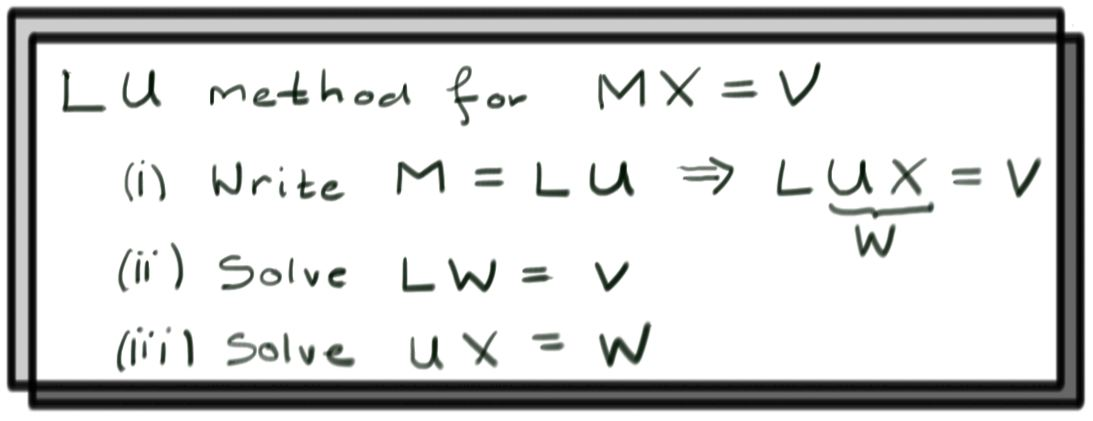
\includegraphics[scale=.3]{\luDecompPath/LU_solution.jpg}
\end{center}
%\end{figure}

\section{Finding an $LU$ Decomposition.}
\label{finding_LU_decomp}
 
For any given matrix, there are actually many different $LU$ decompositions.  However, there is a unique $LU$ decomposition in which the $L$ matrix has ones on the diagonal. In that case $L$ is called a \emph{lower unit triangular matrix}\index{Lower unit triangular matrix}.

To find the $LU$ decomposition, we'll create two sequences of matrices $L_0, L_1, \ldots$ and $U_0, U_1, \ldots$ such that at each step, $L_iU_i=M$.  Each of the $L_i$ will be lower triangular, but only the last $U_i$ will be upper triangular.

Start by setting $L_0=I$ and $U_0=M$, because $L_0U_0=M$. A main concept of this calculation is captured by the following example:

\begin{example}
Consider $$E=\begin{pmatrix}1&0\\\lambda&1\end{pmatrix}\, ,\qquad M=\begin{pmatrix}a&b&c&\cdots\\d&e&f&\cdots\end{pmatrix}\, .$$
Lets compute $EM$
$$
EM=\begin{pmatrix}a&b&c&\cdots\\d+\lambda a&e+\lambda b&f+\lambda c&\cdots\end{pmatrix}\, ,.
$$
Something neat happened here: multiplying $M$ by $E$ performed the row operation $R_2\to R_2+\lambda R-1$ on $M$.
Another interesting fact:
$$
E^{-1}:=\begin{pmatrix}1&0\\-\lambda&1\end{pmatrix}
$$ 
obeys (check this yourself...)
$$
E^{-1} E = 1\, .
$$
Hence $M=E^{-1} E M$ or, writing this out
$$
\begin{pmatrix}a&b&c&\cdots\\d&e&f&\cdots\end{pmatrix}=\begin{pmatrix}1&0\\-\lambda&1\end{pmatrix} \begin{pmatrix}a&b&c&\cdots\\d+\lambda a&e+\lambda b&f+\lambda c&\cdots\end{pmatrix}\, .
$$
Here the matrix on the left is lower triangular, while the matrix on the right has had a row operation performed on it.
\end{example}




\vspace{2mm}
We would like to  use the first row of $U_0$ to zero out the first entry of every row below it.  For our running example, $$U_0=M=\begin{pmatrix}
6 & 18 & 3 \\
2 & 12 & 1 \\
4 & 15 & 3 
\end{pmatrix}\, ,$$ so we would like to perform the row operations $R_2\to R_2 -\frac 13 R_1$ and $R_3\to R_3-\frac 23R_1$.
%so the second row minus $\frac{1}{3}$ of the first row will zero out the first entry in the second row.  Likewise, the third row minus $\frac{2}{3}$ of the first row will zero out the first entry in the third row.
If we perform these row operations on $U_0$ to produce 
$$U_1=\begin{pmatrix}
6 & 18 & 3 \\
0 & 6 & 0 \\
0 & 3 & 1 
\end{pmatrix}\, ,$$
we need to multiply this on the left by a lower triangular matrix $L_1$ so that the product $L_1U_1=M$ still.
The above example shows how to do this:
Set $L_1$ to be the lower triangular matrix whose first column is filled with the minus constants used to zero out the first column of $M$.  Then $$L_1 = \begin{pmatrix}
1 & 0 & 0 \\[1mm]
\frac{1}{3} & 1 & 0 \\[1mm]
\frac{2}{3} & 0 & 1 
\end{pmatrix}\, .$$  
%Set $U_1$ to be the matrix obtained by zeroing out the first column of $M$.  Then $U_1=\begin{pmatrix}
%6 & 18 & 3 \\
%0 & 6 & 0 \\
%0 & 3 & 1 
%\end{pmatrix}$.
By construction $L_1 U_1=M$, but you should compute this yourself as a double check.

Now repeat the process by zeroing the second column of $U_1$ below the diagonal using the second row of $U_1$ using the row operation
$R_3\to R_3-\frac 12 R_2$ to produce
$$U_2=\begin{pmatrix}6&18&3\\0&6&0\\0&0&1\end{pmatrix}\, .$$
The matrix that undoes this row operation is obtained in the same way we found $L_1$ above and is:
$$
\begin{pmatrix}
1&0&0\\
0&1&0\\
0&\frac 12& 0
\end{pmatrix}\, .
$$
Thus our answer for $L_2$ is the product of this matrix with $L_1$, namely
$$
L_2=
\begin{pmatrix}
1 & 0 & 0 \\[1mm]
\frac{1}{3} & 1 & 0 \\[1mm]
\frac{2}{3} & 0 & 1 
\end{pmatrix}\begin{pmatrix}
1&0&0\\
0&1&0\\
0&\frac 12& 0
\end{pmatrix}
=\begin{pmatrix}
1 & 0 & 0 \\[1mm]
\frac{1}{3} & 1 & 0 \\[1mm]
\frac{2}{3} & \frac{1}{2} & 1 
\end{pmatrix}\, .
$$
Notice that it is lower triangular because 

\begin{center}
\textcolor{brown}{THE PRODUCT OF LOWER TRIANGULAR MATRICES IS ALWAYS LOWER TRIANGULAR!}
\end{center}

\noindent
Moreover it is obtained by recording minus the constants used for all our row operations in the appropriate columns (this always works this way).
Moreover, $U_2$ is upper triangular and $M=L_2U_2$, we are done!
Putting this all together we have
$$M=\begin{pmatrix}
6 & 18 & 3 \\
2 & 12 & 1 \\
4 & 15 & 3 
\end{pmatrix}= \begin{pmatrix}
1 & 0 & 0 \\[1mm]
\frac{1}{3} & 1 & 0 \\[1mm]
\frac{2}{3} & \frac{1}{2} & 1 
\end{pmatrix}\begin{pmatrix}
6 & 18 & 3 \\
0 & 6 & 0 \\
0 & 0 & 1 
\end{pmatrix}\, .$$  
%Since $U_2$ is upper-triangular, we're done.  Inserting the new number into $L_1$ to get $L_2$ really is safe: the numbers in the first column don't affect the second column of $U_1$, since the first column of $U_1$ is already zeroed out.

If the matrix you're working with has more than three rows, just continue this process by zeroing out the next column below the diagonal, and repeat until there's nothing left to do.

\videoscriptlink{lu_decomposition_example.mp4}{Another $LU$ decomposition example}{scripts_lu_decomposition_example}

The fractions in the $L$ matrix are admittedly ugly.  For two matrices $LU$, we can multiply one entire column of $L$ by a constant $\lambda$ and divide the corresponding row of $U$ by the same constant without changing the product of the two matrices.  Then:

\begin{eqnarray*}
LU &=& \begin{pmatrix}
1 & 0 & 0 \\[1mm]
\frac{1}{3} & 1 & 0 \\[1mm]
\frac{2}{3} & \frac{1}{2} & 1 
\end{pmatrix}
I
\begin{pmatrix}
6 & 18 & 3 \\
0 & 6 & 0 \\
0 & 0 & 1 
\end{pmatrix} \\
&=&
\begin{pmatrix}
1 & 0 & 0 \\[1mm]
\frac{1}{3} & 1 & 0 \\[1mm]
\frac{2}{3} & \frac{1}{2} & 1 
\end{pmatrix}
\begin{pmatrix}
3 & 0 & 0 \\
0 & 6 & 0 \\
0 & 0 & 1 
\end{pmatrix}
\begin{pmatrix}
\frac{1}{3} & 0 & 0 \\[1mm]
0 & \frac{1}{6} & 0 \\[1mm]
0 & 0 & 1 
\end{pmatrix}
\begin{pmatrix}
6 & 18 & 3 \\
0 & 6 & 0 \\
0 & 0 & 1 
\end{pmatrix} \\
&=&
\begin{pmatrix}
3 & 0 & 0 \\
1 & 6 & 0 \\
2 & 3 & 1 
\end{pmatrix}\begin{pmatrix}
2 & 6 & 1 \\
0 & 1 & 0 \\
0 & 0 & 1 
\end{pmatrix}.
\end{eqnarray*}
The resulting matrix looks nicer, but isn't in standard (lower unit triangular matrix) form.

\reading{11}{2}
%\href{\webworkurl ReadingHomework11/2/}{Reading homework: problem 11.2}

For matrices that are not square, $LU$ decomposition still makes sense.  Given an $m\times n$ matrix $M$, for example we could write $M=LU$ with $L$ a square lower unit triangular matrix, and $U$ a rectangular matrix.  Then $L$ will be an $m\times m$ matrix, and $U$ will be an $m\times n$ matrix (of the same shape as $M$).  From here, the process is exactly the same as for a square matrix.  We create a sequence of matrices $L_i$ and $U_i$ that is eventually the $LU$ decomposition.  Again, we start with $L_0=I$ and $U_0=M$.

\begin{example}
Let's find the $LU$ decomposition of $M=U_0=\begin{pmatrix}
-2 & 1 & 3 \\
-4 & 4 & 1 
\end{pmatrix}$.  Since $M$ is a $2\times 3$ matrix, our decomposition will consist of a $2\times 2$ matrix and a $2\times 3$ matrix.  Then we start with $L_0=I_2=\begin{pmatrix}
1 & 0 \\
0 & 1
\end{pmatrix}$.

The next step is to zero-out the first column of $M$ below the diagonal.  There is only one row to cancel, then, and it can be removed by subtracting $2$ times the first row of $M$ to the second row of $M$.  Then:

\[
L_1=\begin{pmatrix}
1 & 0 \\
2 & 1
\end{pmatrix}, \qquad 
U_1 = \begin{pmatrix}
-2 & 1 & 3 \\
0 & 2 & -5 
\end{pmatrix}
\]
Since $U_1$ is upper triangular, we're done.  With a larger matrix, we would just continue the process.
\end{example}





\section{Block $LDU$ Decomposition}

Let $M$ be a square block matrix with square blocks $X,Y,Z,W$ such that $X^{-1}$ exists.  Then $M$ can be decomposed as a block $LDU$ decomposition, where $D$ is block diagonal, as follows:
\[
M=\begin{pmatrix}
X & Y \\
Z & W
\end{pmatrix}
\]

Then: \[M=\begin{pmatrix}
I &  0 \\
ZX^{-1} & I
\end{pmatrix}\begin{pmatrix}
X & 0 \\
0 & W-ZX^{-1}Y
\end{pmatrix}\begin{pmatrix}
I & X^{-1}Y \\
0 & I
\end{pmatrix}.\]
This can be checked explicitly simply by block-multiplying these three matrices.

\videoscriptlink{lu_decomposition_blocks.mp4}{Block $LDU$ Explanation}{scripts_lu_decomposition_blocks}

\begin{example}
For a $2\times 2$ matrix, we can regard each entry as a block.
\[
\begin{pmatrix}
1 & 2 \\
3 & 4
\end{pmatrix}=
\begin{pmatrix}
1 & 0 \\
3 & 1
\end{pmatrix}
\begin{pmatrix}
1 & 0 \\
0 & -2
\end{pmatrix}
\begin{pmatrix}
1 & 2 \\
0 & 1
\end{pmatrix}
\]
By multiplying the diagonal matrix by the upper triangular matrix, we get the standard $LU$ decomposition of the matrix.
\end{example}


%\section*{References}
%Wikipedia:
%\begin{itemize}
%\item \href{http://en.wikipedia.org/wiki/LU_decomposition}{$LU$ Decomposition}
%\item \href{http://en.wikipedia.org/wiki/Block_LU_decomposition}{Block $LU$ Decomposition}
%\end{itemize}

\section{Review Problems}



\begin{enumerate}

\item Let $D=\begin{pmatrix}
\lambda_1 & \mc0 \\
\mc0 & \lambda_2 \\
\end{pmatrix}$.
\begin{enumerate}
\item Write $D$ in terms of the vectors $e_1$ and $e_2$, and their transposes.
\item Suppose $P=\begin{pmatrix}
a & b \\
c & d \\
\end{pmatrix}$ is invertible.  Show that $D$ is similar to
\[
M=\frac{1}{ad-bc}\begin{pmatrix}
\lambda_1ad-\lambda_2bc & -(\lambda_1-\lambda_2)ab \\[1mm]
(\lambda_1-\lambda_2)cd & -\lambda_1bc + \lambda_2ad
\end{pmatrix}.
\]
\item Suppose the vectors $\rowvec{a,b}$ and $\rowvec{c,d}$ are orthogonal.  What can you say about $M$ in this case? (Hint: think about what \(M^T\) is equal to.)
\end{enumerate}

\phantomnewpage

\item \label{orthogprob} Suppose $S=\{v_1, \ldots, v_n \}$ is an \emph{orthogonal} (not orthonormal) basis for~$\Re^n$.  Then we can write any vector $v$ as $v=\sum_ic^iv_i$ for some constants $c^i$.  Find a formula for the constants $c^i$ in terms of $v$ and the vectors in~$S$.

\Videoscriptlink{orthonormal_bases_hint.mp4}{Hint}{scripts_orthonormal_bases_hint}
\phantomnewpage

\item \label{orthogprojprob} Let $u,v$ be linearly independent vectors in $\Re^3$, and $P=\spa \{ u,v\}$ be the plane spanned by $u$ and $v$.  
\begin{enumerate}
\item Is the vector $v^\bot := v-\frac{u\cdot v}{u\cdot u}u$ in the plane $P$?
\item  What is the (cosine of the) angle between $v^\bot$ and $u$?
\item %Given your solution to the above, 
How can you find a third vector perpendicular to both $u$ and $v^\bot$?
\item  Construct an orthonormal basis for $\Re^3$ from $u$ and $v$.
\item  Test your abstract formul\ae\ starting with 
\[
u=\rowvec{1 , 2 , 0} \text{ and } v=\rowvec{0 , 1 , 1}.
\]
\end{enumerate}

\Videoscriptlink{orthonormal_bases_hint3.mp4}{Hint}{scripts_orthonormal_bases_hint3}

\phantomnewpage



\item Find an orthonormal  basis for $\Re^4$ which includes $(1,1,1,1)$ using the following procedure:\\
\begin{enumerate} 
\item Pick a vector perpendicular to the vector 
$$v_1 =\colvec{1\\1\\1\\1}$$ from the solution set of the matrix equation $$v_1^Tx=0\, .$$ Pick the vector $v_2$ obtained from the standard Gaussian elimination procedure which is the coefficient of $x_2$.
\item Pick a vector perpendicular to both $v_1$ and $v_2$ from the solutions set of the matrix equation $$\colvec{v_1^T\\[1mm]v_2^T}x=0\, .$$ Pick the vector $v_3$ obtained from the standard Gaussian elimination procedure with $x_3$ as the coefficient. 
\item Pick a vector perpendicular to $v_1,v_2,$ and $v_3$ from the solution set of the matrix equation $$\colvec{v_1^T\\[1mm]v_2^T\\[1mm]v_3^T}x=0\, .$$  Pick the vector $v_4$ obtained from the standard Gaussian elimination procedure with $x_3$ as the coefficient. 
\item Normalize the four vectors obtained   above.
\end{enumerate}


\item Use the inner product $$f\cdot g := \int_0^1 f(x)g(x)dx$$  on the vector space $V={\rm span} \{1,x,x^2,x^3\}$ to perform the Gram-Schmidt procedure on the set of vectors $\{1,x,x^2,x^3\}$. 

\item Use the inner product $$f\cdot g := \int_0^{2\pi} f(x)g(x)dx$$  on the vector space $V={\rm span} \{\sin(x),\sin(2x),\sin(3x) \}$ to perform the Gram-Schmidt procedure on the set of vectors $\{\sin(x),\sin(2x),\sin(3x) \}$. \\
Try to build an orthonormal basis for the vector space $$\spa \{ \sin(nx)~| ~n\in \N \}\, .$$
%What do you suspect about the vector space $\spa \{ \sin(nx)~| ~n\in \N \}$?\\
%What do you suspect about the vector space $\spa \{ \sin(ax)~|~ a \in \Re \}$?
\item 
\begin{enumerate}
\item
Show that if $Q$ is an orthogonal $n\times n$ matrix, then $$u\dotprod v = (Qu)\dotprod (Qv)\, ,$$ for any $u,v\in \Re^n$. That is, $Q$ preserves the inner product. 
\item Does $Q$ preserve the outer product? 
\item  If the set of vectors $\{ u_1,\dots,u_n\}$ is orthonormal and $\{ \lambda_1,\cdots,\lambda_n\}$ is a set of numbers, 
then what are the eigenvalues and eigenvectors of the matrix
$M=\sum_{i=1}^n \lambda_i u_i u_i^T$? 
\item How would the eigenvectors and eigenvalues of this matrix change if we replaced  $\{ u_1,\dots,u_n\}$ by $\{ Qu_1,\dots,Q u_n\}$?
\end{enumerate}


\item Carefully write out the Gram-Schmidt procedure for the set of vectors 
$$\left\{ \colvec{1\\1\\1}, \colvec{1\\-1\\1}, \colvec{1\\1\\-1} \right\} \, .$$ Is it possible to rescale the second vector obtained in the procedure to a vector with integer components? 


\item 
\label{basisortho}
\begin{enumerate}
\item Suppose $u$ and $v$ are linearly independent.  Show that $u$ and $v^\perp$ are also linearly independent.  Explain why $\{u, v^\perp\}$ is a basis for $\spa \{u,v\}$.



\Videoscriptlink{gram_schmidt_and_orthogonal_complements_hint.mp4}{Hint}{gram_schmidt_and_orthogonal_complements_hint}

\item Repeat the previous problem, but with three independent vectors $u,v,w$
 where $v^\perp$ and $w^\perp$ are as defined by the Gram-Schmidt procedure. 
\end{enumerate}

\phantomnewpage


\item \label{QRprob} Find the $QR$ factorization of
$$
M=\begin{pmatrix}1&0&\phantom{\!-}2\\-1&2&0\\-1&-2&2
\end{pmatrix}\, .
$$

\phantomnewpage

\item Given any three vectors $u,v,w$, when do $v^\perp$ or $w^\perp$ of the Gram--Schmidt procedure vanish?

\phantomnewpage

\item For $U$ a subspace of $W$, use the subspace theorem to check that $U^\perp$ is a subspace of $W$.

\phantomnewpage


\phantomnewpage

\item %(Extra Credit) 
Let $S_n$ and $A_n$ define the space of $n \times n$ symmetric and anti-symmetric matrices, respectively. These are subspaces of the vector space $M^n_n$ of all $n\times n$ matrices. What is $\dim M^n_n$, $\dim S_n$, and $\dim A_n$? Show that $M^n_n = S_n + A_n$. Define an inner product on square matrices
$$
M\cdot N ={\rm tr} MN\, .
$$
Is $A_n^{\perp}=S_n$? Is $M^n_n = S_n \oplus A_n$?

%\emph{Hint: Note that $\dim S_n = \dim U_n$ where $U_n$ is the vector space of all $n \times n$ upper triangular matrices, and also note that $\dim A_n = \dim \widetilde{U}_n$ where $\widetilde{U}_n$ is the vector space of all strictly $n \times n$ upper triangular matrices (\emph{i.e.} the diagonal entries are all 0).}

\item The vector space $V={\rm span} \{ \sin(t),\sin(2t), \sin(3t) , \sin(3t)\}$ has an inner product: 
$$f\cdot g:=\int _0^{2\pi}f(t)g(t) dt\, .$$ Find the orthogonal compliment to $U={\rm span} \{ \sin(t)+\sin(2t) \}$ in $V$. Express $\sin(t)-\sin(2t)$ as  the sum of vectors from $U$ and $U^\perp$.

\end{enumerate}

\phantomnewpage

\newpage

%%To do: The section on solution sets might be too redundant, and then again might be good with more of a geometric interpretation emphasis.



%include these for summer 2013 version:
%\chapter{\luDecompTitle}
\label{LUdecomp}

Certain matrices are easier to work with than others.  In this section, we will see how to write any square\footnote{The case where $M$ is not square is dealt with at the end of the lecture.} matrix $M$ as the product of two simpler matrices.  We will write $$M=LU\, ,$$ where:
\begin{itemize}
\item $L$ is \emph{lower triangular}\index{Lower triangular matrix}.  This means that all entries above the main diagonal are zero.  In notation,
$L=(l^i_j)$ with $l^i_j=0$ for all $j>i$.
\[L=\begin{pmatrix}
l^1_1 & 0 & 0 & \cdots \\
l^2_1 & l^2_2 & 0 & \cdots \\
l^3_1 & l^3_2 & l^3_3 & \cdots \\
\vdots & \vdots & \vdots & \ddots \\
\end{pmatrix}
\]

\item $U$ is \emph{upper triangular}\index{Upper triangular matrix}.  This means that all entries below the main diagonal are zero.  In notation,
$U=(u^i_j)$ with $u^i_j=0$ for all $j<i$.
\[U=\begin{pmatrix}
u^1_1 & u^1_2 & u^1_3 & \cdots \\
0 & u^2_2 & u^2_3 & \cdots \\
0 & 0 & u^3_3 & \cdots \\
\vdots & \vdots & \vdots & \ddots \\
\end{pmatrix}
\]
\end{itemize}
$M=LU$ is called an \emph{$LU$ decomposition}\index{LU@$LU$ decomposition} of $M$.

This is a useful trick for  computational reasons; it is much easier to compute the inverse of an upper or lower triangular matrix than general matrices.  Since inverses are useful for solving linear systems, this makes solving any linear system associated to the matrix much faster as well.  The determinant---a very important quantity associated with any square matrix---is very easy to compute for triangular matrices.

\begin{example}
Linear systems associated to upper triangular matrices are very easy to solve by back substitution.
\[
\begin{amatrix}{2}
a & b & 1 \\
0 & c & e \\
\end{amatrix} \ \Rightarrow \ y=\frac{e}{c}\, , \quad x=\frac{1}{a}\left(1-\frac{be}{c}\right)
\]

\[
\begin{amatrix}{3}
1 & 0 & 0 & d \\
a & 1 & 0 & e \\
b & c & 1 & f \\
\end{amatrix} \Rightarrow x=d\, , \qquad y=e-ad\, , \qquad z=f-bd-c(e-ad)
\]
For lower triangular matrices, \emph{back} substitution\index{Back substitution} gives a quick solution; for upper triangular matrices, \emph{forward} substitution\index{Forward substitution} gives the solution.
\end{example}





\section{Using $LU$ Decomposition to Solve Linear Systems}

Suppose we have $M=LU$ and want to solve the system
\[
MX=LUX=V.
\]

\begin{itemize}
\item{Step 1:} Set $W=\colvec{u\\v\\w}=UX$.  

\item{Step 2:} Solve the system $LW=V$.  This should be simple by forward substitution since $L$ is lower triangular.  Suppose the solution to $LW=V$ is $W_0$.  

\item{Step 3:} Now solve the system $UX=W_0$.  This should be easy by backward substitution, since $U$ is upper triangular.  The solution to this system is the solution to the original system.
\end{itemize}
We can think of this as using the matrix $L$ to perform row operations on the matrix $U$ in order to solve the system; this idea also appears in the  study of determinants.

%\href{\webworkurl ReadingHomework11/1/}{Reading homework: problem 11.1}
\reading{11}{1}

\begin{example}
Consider the linear system:
\[
      \begin{linsys}{4}
            6x & +&18y & +&3z         &=& 3  \\[1mm]
            2x & +&12y & +&z	    &=& 19 \\[1mm]
            4x & +&15y & +&3z         &=& 0  
      \end{linsys}
\]

An $LU$ decomposition for the associated matrix $M$ is:
\[
\begin{pmatrix}
6 & 18 & 3 \\
2 & 12 & 1 \\
4 & 15 & 3 
\end{pmatrix} =
\begin{pmatrix}
3 & 0 & 0 \\
1 & 6 & 0 \\
2 & 3 & 1 
\end{pmatrix}
\begin{pmatrix}
2 & 6 & 1 \\
0 & 1 & 0 \\
0 & 0 & 1 
\end{pmatrix}.
\]

\begin{itemize}
\item{Step 1:} \hypertarget{LUproc}{Set} $W=\colvec{u\\v\\w}=UX$.  

\item{Step 2:} Solve the system $LW=V$:

\[
\begin{pmatrix}
3 & 0 & 0 \\
1 & 6 & 0 \\
2 & 3 & 1 
\end{pmatrix}
\colvec{u\\v\\w} =
\colvec{3\\19\\0}
\]

By substitution, we get $u=1$, $v=3$, and $w=-11$.  Then 
\[W_0=\colvec{1\\3\\-11}\]

\item{Step 3:} Solve the system $UX=W_0$.  
\[
\begin{pmatrix}
2 & 6 & 1 \\
0 & 1 & 0 \\
0 & 0 & 1 
\end{pmatrix}
\colvec{x\\y\\z} =
\colvec{1\\3\\-11}
\]
Back substitution gives $z=-11, y=3$, and $x=-3$.  

Then $X=\colvec{-3\\3\\-11}$, and we're done.
\end{itemize}
\end{example}

\videoscriptlink{lu_decomposition_using_lu_decomp.mp4}{Using a $LU$ decomposition}{scripts_lu_decomposition_using_lu_example}

%\begin{figure}
\begin{center}
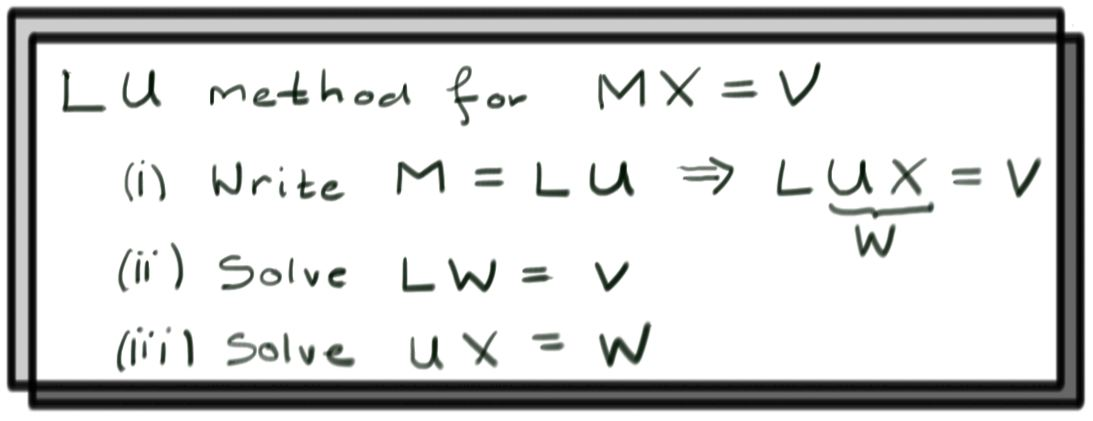
\includegraphics[scale=.3]{\luDecompPath/LU_solution.jpg}
\end{center}
%\end{figure}

\section{Finding an $LU$ Decomposition.}
\label{finding_LU_decomp}
 
For any given matrix, there are actually many different $LU$ decompositions.  However, there is a unique $LU$ decomposition in which the $L$ matrix has ones on the diagonal. In that case $L$ is called a \emph{lower unit triangular matrix}\index{Lower unit triangular matrix}.

To find the $LU$ decomposition, we'll create two sequences of matrices $L_0, L_1, \ldots$ and $U_0, U_1, \ldots$ such that at each step, $L_iU_i=M$.  Each of the $L_i$ will be lower triangular, but only the last $U_i$ will be upper triangular.

Start by setting $L_0=I$ and $U_0=M$, because $L_0U_0=M$. A main concept of this calculation is captured by the following example:

\begin{example}
Consider $$E=\begin{pmatrix}1&0\\\lambda&1\end{pmatrix}\, ,\qquad M=\begin{pmatrix}a&b&c&\cdots\\d&e&f&\cdots\end{pmatrix}\, .$$
Lets compute $EM$
$$
EM=\begin{pmatrix}a&b&c&\cdots\\d+\lambda a&e+\lambda b&f+\lambda c&\cdots\end{pmatrix}\, ,.
$$
Something neat happened here: multiplying $M$ by $E$ performed the row operation $R_2\to R_2+\lambda R-1$ on $M$.
Another interesting fact:
$$
E^{-1}:=\begin{pmatrix}1&0\\-\lambda&1\end{pmatrix}
$$ 
obeys (check this yourself...)
$$
E^{-1} E = 1\, .
$$
Hence $M=E^{-1} E M$ or, writing this out
$$
\begin{pmatrix}a&b&c&\cdots\\d&e&f&\cdots\end{pmatrix}=\begin{pmatrix}1&0\\-\lambda&1\end{pmatrix} \begin{pmatrix}a&b&c&\cdots\\d+\lambda a&e+\lambda b&f+\lambda c&\cdots\end{pmatrix}\, .
$$
Here the matrix on the left is lower triangular, while the matrix on the right has had a row operation performed on it.
\end{example}




\vspace{2mm}
We would like to  use the first row of $U_0$ to zero out the first entry of every row below it.  For our running example, $$U_0=M=\begin{pmatrix}
6 & 18 & 3 \\
2 & 12 & 1 \\
4 & 15 & 3 
\end{pmatrix}\, ,$$ so we would like to perform the row operations $R_2\to R_2 -\frac 13 R_1$ and $R_3\to R_3-\frac 23R_1$.
%so the second row minus $\frac{1}{3}$ of the first row will zero out the first entry in the second row.  Likewise, the third row minus $\frac{2}{3}$ of the first row will zero out the first entry in the third row.
If we perform these row operations on $U_0$ to produce 
$$U_1=\begin{pmatrix}
6 & 18 & 3 \\
0 & 6 & 0 \\
0 & 3 & 1 
\end{pmatrix}\, ,$$
we need to multiply this on the left by a lower triangular matrix $L_1$ so that the product $L_1U_1=M$ still.
The above example shows how to do this:
Set $L_1$ to be the lower triangular matrix whose first column is filled with the minus constants used to zero out the first column of $M$.  Then $$L_1 = \begin{pmatrix}
1 & 0 & 0 \\[1mm]
\frac{1}{3} & 1 & 0 \\[1mm]
\frac{2}{3} & 0 & 1 
\end{pmatrix}\, .$$  
%Set $U_1$ to be the matrix obtained by zeroing out the first column of $M$.  Then $U_1=\begin{pmatrix}
%6 & 18 & 3 \\
%0 & 6 & 0 \\
%0 & 3 & 1 
%\end{pmatrix}$.
By construction $L_1 U_1=M$, but you should compute this yourself as a double check.

Now repeat the process by zeroing the second column of $U_1$ below the diagonal using the second row of $U_1$ using the row operation
$R_3\to R_3-\frac 12 R_2$ to produce
$$U_2=\begin{pmatrix}6&18&3\\0&6&0\\0&0&1\end{pmatrix}\, .$$
The matrix that undoes this row operation is obtained in the same way we found $L_1$ above and is:
$$
\begin{pmatrix}
1&0&0\\
0&1&0\\
0&\frac 12& 0
\end{pmatrix}\, .
$$
Thus our answer for $L_2$ is the product of this matrix with $L_1$, namely
$$
L_2=
\begin{pmatrix}
1 & 0 & 0 \\[1mm]
\frac{1}{3} & 1 & 0 \\[1mm]
\frac{2}{3} & 0 & 1 
\end{pmatrix}\begin{pmatrix}
1&0&0\\
0&1&0\\
0&\frac 12& 0
\end{pmatrix}
=\begin{pmatrix}
1 & 0 & 0 \\[1mm]
\frac{1}{3} & 1 & 0 \\[1mm]
\frac{2}{3} & \frac{1}{2} & 1 
\end{pmatrix}\, .
$$
Notice that it is lower triangular because 

\begin{center}
\textcolor{brown}{THE PRODUCT OF LOWER TRIANGULAR MATRICES IS ALWAYS LOWER TRIANGULAR!}
\end{center}

\noindent
Moreover it is obtained by recording minus the constants used for all our row operations in the appropriate columns (this always works this way).
Moreover, $U_2$ is upper triangular and $M=L_2U_2$, we are done!
Putting this all together we have
$$M=\begin{pmatrix}
6 & 18 & 3 \\
2 & 12 & 1 \\
4 & 15 & 3 
\end{pmatrix}= \begin{pmatrix}
1 & 0 & 0 \\[1mm]
\frac{1}{3} & 1 & 0 \\[1mm]
\frac{2}{3} & \frac{1}{2} & 1 
\end{pmatrix}\begin{pmatrix}
6 & 18 & 3 \\
0 & 6 & 0 \\
0 & 0 & 1 
\end{pmatrix}\, .$$  
%Since $U_2$ is upper-triangular, we're done.  Inserting the new number into $L_1$ to get $L_2$ really is safe: the numbers in the first column don't affect the second column of $U_1$, since the first column of $U_1$ is already zeroed out.

If the matrix you're working with has more than three rows, just continue this process by zeroing out the next column below the diagonal, and repeat until there's nothing left to do.

\videoscriptlink{lu_decomposition_example.mp4}{Another $LU$ decomposition example}{scripts_lu_decomposition_example}

The fractions in the $L$ matrix are admittedly ugly.  For two matrices $LU$, we can multiply one entire column of $L$ by a constant $\lambda$ and divide the corresponding row of $U$ by the same constant without changing the product of the two matrices.  Then:

\begin{eqnarray*}
LU &=& \begin{pmatrix}
1 & 0 & 0 \\[1mm]
\frac{1}{3} & 1 & 0 \\[1mm]
\frac{2}{3} & \frac{1}{2} & 1 
\end{pmatrix}
I
\begin{pmatrix}
6 & 18 & 3 \\
0 & 6 & 0 \\
0 & 0 & 1 
\end{pmatrix} \\
&=&
\begin{pmatrix}
1 & 0 & 0 \\[1mm]
\frac{1}{3} & 1 & 0 \\[1mm]
\frac{2}{3} & \frac{1}{2} & 1 
\end{pmatrix}
\begin{pmatrix}
3 & 0 & 0 \\
0 & 6 & 0 \\
0 & 0 & 1 
\end{pmatrix}
\begin{pmatrix}
\frac{1}{3} & 0 & 0 \\[1mm]
0 & \frac{1}{6} & 0 \\[1mm]
0 & 0 & 1 
\end{pmatrix}
\begin{pmatrix}
6 & 18 & 3 \\
0 & 6 & 0 \\
0 & 0 & 1 
\end{pmatrix} \\
&=&
\begin{pmatrix}
3 & 0 & 0 \\
1 & 6 & 0 \\
2 & 3 & 1 
\end{pmatrix}\begin{pmatrix}
2 & 6 & 1 \\
0 & 1 & 0 \\
0 & 0 & 1 
\end{pmatrix}.
\end{eqnarray*}
The resulting matrix looks nicer, but isn't in standard (lower unit triangular matrix) form.

\reading{11}{2}
%\href{\webworkurl ReadingHomework11/2/}{Reading homework: problem 11.2}

For matrices that are not square, $LU$ decomposition still makes sense.  Given an $m\times n$ matrix $M$, for example we could write $M=LU$ with $L$ a square lower unit triangular matrix, and $U$ a rectangular matrix.  Then $L$ will be an $m\times m$ matrix, and $U$ will be an $m\times n$ matrix (of the same shape as $M$).  From here, the process is exactly the same as for a square matrix.  We create a sequence of matrices $L_i$ and $U_i$ that is eventually the $LU$ decomposition.  Again, we start with $L_0=I$ and $U_0=M$.

\begin{example}
Let's find the $LU$ decomposition of $M=U_0=\begin{pmatrix}
-2 & 1 & 3 \\
-4 & 4 & 1 
\end{pmatrix}$.  Since $M$ is a $2\times 3$ matrix, our decomposition will consist of a $2\times 2$ matrix and a $2\times 3$ matrix.  Then we start with $L_0=I_2=\begin{pmatrix}
1 & 0 \\
0 & 1
\end{pmatrix}$.

The next step is to zero-out the first column of $M$ below the diagonal.  There is only one row to cancel, then, and it can be removed by subtracting $2$ times the first row of $M$ to the second row of $M$.  Then:

\[
L_1=\begin{pmatrix}
1 & 0 \\
2 & 1
\end{pmatrix}, \qquad 
U_1 = \begin{pmatrix}
-2 & 1 & 3 \\
0 & 2 & -5 
\end{pmatrix}
\]
Since $U_1$ is upper triangular, we're done.  With a larger matrix, we would just continue the process.
\end{example}





\section{Block $LDU$ Decomposition}

Let $M$ be a square block matrix with square blocks $X,Y,Z,W$ such that $X^{-1}$ exists.  Then $M$ can be decomposed as a block $LDU$ decomposition, where $D$ is block diagonal, as follows:
\[
M=\begin{pmatrix}
X & Y \\
Z & W
\end{pmatrix}
\]

Then: \[M=\begin{pmatrix}
I &  0 \\
ZX^{-1} & I
\end{pmatrix}\begin{pmatrix}
X & 0 \\
0 & W-ZX^{-1}Y
\end{pmatrix}\begin{pmatrix}
I & X^{-1}Y \\
0 & I
\end{pmatrix}.\]
This can be checked explicitly simply by block-multiplying these three matrices.

\videoscriptlink{lu_decomposition_blocks.mp4}{Block $LDU$ Explanation}{scripts_lu_decomposition_blocks}

\begin{example}
For a $2\times 2$ matrix, we can regard each entry as a block.
\[
\begin{pmatrix}
1 & 2 \\
3 & 4
\end{pmatrix}=
\begin{pmatrix}
1 & 0 \\
3 & 1
\end{pmatrix}
\begin{pmatrix}
1 & 0 \\
0 & -2
\end{pmatrix}
\begin{pmatrix}
1 & 2 \\
0 & 1
\end{pmatrix}
\]
By multiplying the diagonal matrix by the upper triangular matrix, we get the standard $LU$ decomposition of the matrix.
\end{example}


%\section*{References}
%Wikipedia:
%\begin{itemize}
%\item \href{http://en.wikipedia.org/wiki/LU_decomposition}{$LU$ Decomposition}
%\item \href{http://en.wikipedia.org/wiki/Block_LU_decomposition}{Block $LU$ Decomposition}
%\end{itemize}

\section{Review Problems}



\begin{enumerate}

\item Let $D=\begin{pmatrix}
\lambda_1 & \mc0 \\
\mc0 & \lambda_2 \\
\end{pmatrix}$.
\begin{enumerate}
\item Write $D$ in terms of the vectors $e_1$ and $e_2$, and their transposes.
\item Suppose $P=\begin{pmatrix}
a & b \\
c & d \\
\end{pmatrix}$ is invertible.  Show that $D$ is similar to
\[
M=\frac{1}{ad-bc}\begin{pmatrix}
\lambda_1ad-\lambda_2bc & -(\lambda_1-\lambda_2)ab \\[1mm]
(\lambda_1-\lambda_2)cd & -\lambda_1bc + \lambda_2ad
\end{pmatrix}.
\]
\item Suppose the vectors $\rowvec{a,b}$ and $\rowvec{c,d}$ are orthogonal.  What can you say about $M$ in this case? (Hint: think about what \(M^T\) is equal to.)
\end{enumerate}

\phantomnewpage

\item \label{orthogprob} Suppose $S=\{v_1, \ldots, v_n \}$ is an \emph{orthogonal} (not orthonormal) basis for~$\Re^n$.  Then we can write any vector $v$ as $v=\sum_ic^iv_i$ for some constants $c^i$.  Find a formula for the constants $c^i$ in terms of $v$ and the vectors in~$S$.

\Videoscriptlink{orthonormal_bases_hint.mp4}{Hint}{scripts_orthonormal_bases_hint}
\phantomnewpage

\item \label{orthogprojprob} Let $u,v$ be linearly independent vectors in $\Re^3$, and $P=\spa \{ u,v\}$ be the plane spanned by $u$ and $v$.  
\begin{enumerate}
\item Is the vector $v^\bot := v-\frac{u\cdot v}{u\cdot u}u$ in the plane $P$?
\item  What is the (cosine of the) angle between $v^\bot$ and $u$?
\item %Given your solution to the above, 
How can you find a third vector perpendicular to both $u$ and $v^\bot$?
\item  Construct an orthonormal basis for $\Re^3$ from $u$ and $v$.
\item  Test your abstract formul\ae\ starting with 
\[
u=\rowvec{1 , 2 , 0} \text{ and } v=\rowvec{0 , 1 , 1}.
\]
\end{enumerate}

\Videoscriptlink{orthonormal_bases_hint3.mp4}{Hint}{scripts_orthonormal_bases_hint3}

\phantomnewpage



\item Find an orthonormal  basis for $\Re^4$ which includes $(1,1,1,1)$ using the following procedure:\\
\begin{enumerate} 
\item Pick a vector perpendicular to the vector 
$$v_1 =\colvec{1\\1\\1\\1}$$ from the solution set of the matrix equation $$v_1^Tx=0\, .$$ Pick the vector $v_2$ obtained from the standard Gaussian elimination procedure which is the coefficient of $x_2$.
\item Pick a vector perpendicular to both $v_1$ and $v_2$ from the solutions set of the matrix equation $$\colvec{v_1^T\\[1mm]v_2^T}x=0\, .$$ Pick the vector $v_3$ obtained from the standard Gaussian elimination procedure with $x_3$ as the coefficient. 
\item Pick a vector perpendicular to $v_1,v_2,$ and $v_3$ from the solution set of the matrix equation $$\colvec{v_1^T\\[1mm]v_2^T\\[1mm]v_3^T}x=0\, .$$  Pick the vector $v_4$ obtained from the standard Gaussian elimination procedure with $x_3$ as the coefficient. 
\item Normalize the four vectors obtained   above.
\end{enumerate}


\item Use the inner product $$f\cdot g := \int_0^1 f(x)g(x)dx$$  on the vector space $V={\rm span} \{1,x,x^2,x^3\}$ to perform the Gram-Schmidt procedure on the set of vectors $\{1,x,x^2,x^3\}$. 

\item Use the inner product $$f\cdot g := \int_0^{2\pi} f(x)g(x)dx$$  on the vector space $V={\rm span} \{\sin(x),\sin(2x),\sin(3x) \}$ to perform the Gram-Schmidt procedure on the set of vectors $\{\sin(x),\sin(2x),\sin(3x) \}$. \\
Try to build an orthonormal basis for the vector space $$\spa \{ \sin(nx)~| ~n\in \N \}\, .$$
%What do you suspect about the vector space $\spa \{ \sin(nx)~| ~n\in \N \}$?\\
%What do you suspect about the vector space $\spa \{ \sin(ax)~|~ a \in \Re \}$?
\item 
\begin{enumerate}
\item
Show that if $Q$ is an orthogonal $n\times n$ matrix, then $$u\dotprod v = (Qu)\dotprod (Qv)\, ,$$ for any $u,v\in \Re^n$. That is, $Q$ preserves the inner product. 
\item Does $Q$ preserve the outer product? 
\item  If the set of vectors $\{ u_1,\dots,u_n\}$ is orthonormal and $\{ \lambda_1,\cdots,\lambda_n\}$ is a set of numbers, 
then what are the eigenvalues and eigenvectors of the matrix
$M=\sum_{i=1}^n \lambda_i u_i u_i^T$? 
\item How would the eigenvectors and eigenvalues of this matrix change if we replaced  $\{ u_1,\dots,u_n\}$ by $\{ Qu_1,\dots,Q u_n\}$?
\end{enumerate}


\item Carefully write out the Gram-Schmidt procedure for the set of vectors 
$$\left\{ \colvec{1\\1\\1}, \colvec{1\\-1\\1}, \colvec{1\\1\\-1} \right\} \, .$$ Is it possible to rescale the second vector obtained in the procedure to a vector with integer components? 


\item 
\label{basisortho}
\begin{enumerate}
\item Suppose $u$ and $v$ are linearly independent.  Show that $u$ and $v^\perp$ are also linearly independent.  Explain why $\{u, v^\perp\}$ is a basis for $\spa \{u,v\}$.



\Videoscriptlink{gram_schmidt_and_orthogonal_complements_hint.mp4}{Hint}{gram_schmidt_and_orthogonal_complements_hint}

\item Repeat the previous problem, but with three independent vectors $u,v,w$
 where $v^\perp$ and $w^\perp$ are as defined by the Gram-Schmidt procedure. 
\end{enumerate}

\phantomnewpage


\item \label{QRprob} Find the $QR$ factorization of
$$
M=\begin{pmatrix}1&0&\phantom{\!-}2\\-1&2&0\\-1&-2&2
\end{pmatrix}\, .
$$

\phantomnewpage

\item Given any three vectors $u,v,w$, when do $v^\perp$ or $w^\perp$ of the Gram--Schmidt procedure vanish?

\phantomnewpage

\item For $U$ a subspace of $W$, use the subspace theorem to check that $U^\perp$ is a subspace of $W$.

\phantomnewpage


\phantomnewpage

\item %(Extra Credit) 
Let $S_n$ and $A_n$ define the space of $n \times n$ symmetric and anti-symmetric matrices, respectively. These are subspaces of the vector space $M^n_n$ of all $n\times n$ matrices. What is $\dim M^n_n$, $\dim S_n$, and $\dim A_n$? Show that $M^n_n = S_n + A_n$. Define an inner product on square matrices
$$
M\cdot N ={\rm tr} MN\, .
$$
Is $A_n^{\perp}=S_n$? Is $M^n_n = S_n \oplus A_n$?

%\emph{Hint: Note that $\dim S_n = \dim U_n$ where $U_n$ is the vector space of all $n \times n$ upper triangular matrices, and also note that $\dim A_n = \dim \widetilde{U}_n$ where $\widetilde{U}_n$ is the vector space of all strictly $n \times n$ upper triangular matrices (\emph{i.e.} the diagonal entries are all 0).}

\item The vector space $V={\rm span} \{ \sin(t),\sin(2t), \sin(3t) , \sin(3t)\}$ has an inner product: 
$$f\cdot g:=\int _0^{2\pi}f(t)g(t) dt\, .$$ Find the orthogonal compliment to $U={\rm span} \{ \sin(t)+\sin(2t) \}$ in $V$. Express $\sin(t)-\sin(2t)$ as  the sum of vectors from $U$ and $U^\perp$.

\end{enumerate}

\phantomnewpage

\newpage

%\chapter{\luDecompTitle}
\label{LUdecomp}

Certain matrices are easier to work with than others.  In this section, we will see how to write any square\footnote{The case where $M$ is not square is dealt with at the end of the lecture.} matrix $M$ as the product of two simpler matrices.  We will write $$M=LU\, ,$$ where:
\begin{itemize}
\item $L$ is \emph{lower triangular}\index{Lower triangular matrix}.  This means that all entries above the main diagonal are zero.  In notation,
$L=(l^i_j)$ with $l^i_j=0$ for all $j>i$.
\[L=\begin{pmatrix}
l^1_1 & 0 & 0 & \cdots \\
l^2_1 & l^2_2 & 0 & \cdots \\
l^3_1 & l^3_2 & l^3_3 & \cdots \\
\vdots & \vdots & \vdots & \ddots \\
\end{pmatrix}
\]

\item $U$ is \emph{upper triangular}\index{Upper triangular matrix}.  This means that all entries below the main diagonal are zero.  In notation,
$U=(u^i_j)$ with $u^i_j=0$ for all $j<i$.
\[U=\begin{pmatrix}
u^1_1 & u^1_2 & u^1_3 & \cdots \\
0 & u^2_2 & u^2_3 & \cdots \\
0 & 0 & u^3_3 & \cdots \\
\vdots & \vdots & \vdots & \ddots \\
\end{pmatrix}
\]
\end{itemize}
$M=LU$ is called an \emph{$LU$ decomposition}\index{LU@$LU$ decomposition} of $M$.

This is a useful trick for  computational reasons; it is much easier to compute the inverse of an upper or lower triangular matrix than general matrices.  Since inverses are useful for solving linear systems, this makes solving any linear system associated to the matrix much faster as well.  The determinant---a very important quantity associated with any square matrix---is very easy to compute for triangular matrices.

\begin{example}
Linear systems associated to upper triangular matrices are very easy to solve by back substitution.
\[
\begin{amatrix}{2}
a & b & 1 \\
0 & c & e \\
\end{amatrix} \ \Rightarrow \ y=\frac{e}{c}\, , \quad x=\frac{1}{a}\left(1-\frac{be}{c}\right)
\]

\[
\begin{amatrix}{3}
1 & 0 & 0 & d \\
a & 1 & 0 & e \\
b & c & 1 & f \\
\end{amatrix} \Rightarrow x=d\, , \qquad y=e-ad\, , \qquad z=f-bd-c(e-ad)
\]
For lower triangular matrices, \emph{back} substitution\index{Back substitution} gives a quick solution; for upper triangular matrices, \emph{forward} substitution\index{Forward substitution} gives the solution.
\end{example}





\section{Using $LU$ Decomposition to Solve Linear Systems}

Suppose we have $M=LU$ and want to solve the system
\[
MX=LUX=V.
\]

\begin{itemize}
\item{Step 1:} Set $W=\colvec{u\\v\\w}=UX$.  

\item{Step 2:} Solve the system $LW=V$.  This should be simple by forward substitution since $L$ is lower triangular.  Suppose the solution to $LW=V$ is $W_0$.  

\item{Step 3:} Now solve the system $UX=W_0$.  This should be easy by backward substitution, since $U$ is upper triangular.  The solution to this system is the solution to the original system.
\end{itemize}
We can think of this as using the matrix $L$ to perform row operations on the matrix $U$ in order to solve the system; this idea also appears in the  study of determinants.

%\href{\webworkurl ReadingHomework11/1/}{Reading homework: problem 11.1}
\reading{11}{1}

\begin{example}
Consider the linear system:
\[
      \begin{linsys}{4}
            6x & +&18y & +&3z         &=& 3  \\[1mm]
            2x & +&12y & +&z	    &=& 19 \\[1mm]
            4x & +&15y & +&3z         &=& 0  
      \end{linsys}
\]

An $LU$ decomposition for the associated matrix $M$ is:
\[
\begin{pmatrix}
6 & 18 & 3 \\
2 & 12 & 1 \\
4 & 15 & 3 
\end{pmatrix} =
\begin{pmatrix}
3 & 0 & 0 \\
1 & 6 & 0 \\
2 & 3 & 1 
\end{pmatrix}
\begin{pmatrix}
2 & 6 & 1 \\
0 & 1 & 0 \\
0 & 0 & 1 
\end{pmatrix}.
\]

\begin{itemize}
\item{Step 1:} \hypertarget{LUproc}{Set} $W=\colvec{u\\v\\w}=UX$.  

\item{Step 2:} Solve the system $LW=V$:

\[
\begin{pmatrix}
3 & 0 & 0 \\
1 & 6 & 0 \\
2 & 3 & 1 
\end{pmatrix}
\colvec{u\\v\\w} =
\colvec{3\\19\\0}
\]

By substitution, we get $u=1$, $v=3$, and $w=-11$.  Then 
\[W_0=\colvec{1\\3\\-11}\]

\item{Step 3:} Solve the system $UX=W_0$.  
\[
\begin{pmatrix}
2 & 6 & 1 \\
0 & 1 & 0 \\
0 & 0 & 1 
\end{pmatrix}
\colvec{x\\y\\z} =
\colvec{1\\3\\-11}
\]
Back substitution gives $z=-11, y=3$, and $x=-3$.  

Then $X=\colvec{-3\\3\\-11}$, and we're done.
\end{itemize}
\end{example}

\videoscriptlink{lu_decomposition_using_lu_decomp.mp4}{Using a $LU$ decomposition}{scripts_lu_decomposition_using_lu_example}

%\begin{figure}
\begin{center}
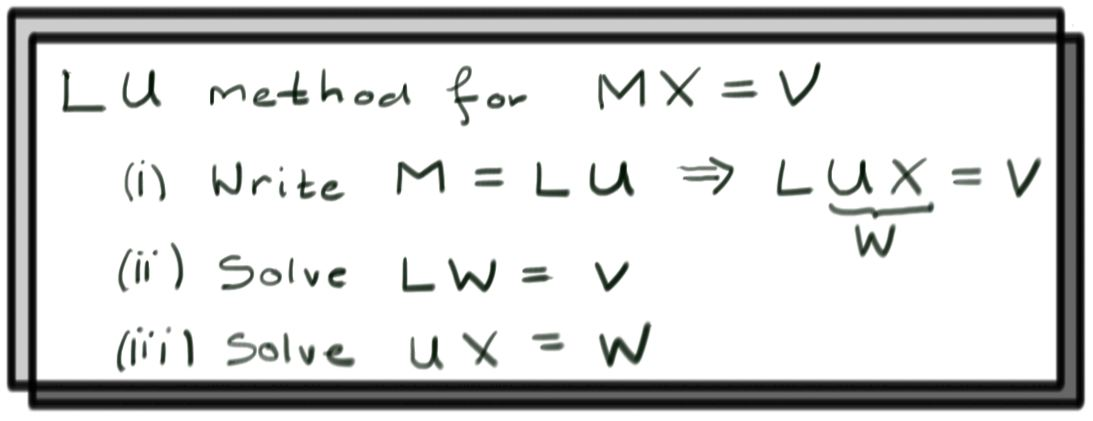
\includegraphics[scale=.3]{\luDecompPath/LU_solution.jpg}
\end{center}
%\end{figure}

\section{Finding an $LU$ Decomposition.}
\label{finding_LU_decomp}
 
For any given matrix, there are actually many different $LU$ decompositions.  However, there is a unique $LU$ decomposition in which the $L$ matrix has ones on the diagonal. In that case $L$ is called a \emph{lower unit triangular matrix}\index{Lower unit triangular matrix}.

To find the $LU$ decomposition, we'll create two sequences of matrices $L_0, L_1, \ldots$ and $U_0, U_1, \ldots$ such that at each step, $L_iU_i=M$.  Each of the $L_i$ will be lower triangular, but only the last $U_i$ will be upper triangular.

Start by setting $L_0=I$ and $U_0=M$, because $L_0U_0=M$. A main concept of this calculation is captured by the following example:

\begin{example}
Consider $$E=\begin{pmatrix}1&0\\\lambda&1\end{pmatrix}\, ,\qquad M=\begin{pmatrix}a&b&c&\cdots\\d&e&f&\cdots\end{pmatrix}\, .$$
Lets compute $EM$
$$
EM=\begin{pmatrix}a&b&c&\cdots\\d+\lambda a&e+\lambda b&f+\lambda c&\cdots\end{pmatrix}\, ,.
$$
Something neat happened here: multiplying $M$ by $E$ performed the row operation $R_2\to R_2+\lambda R-1$ on $M$.
Another interesting fact:
$$
E^{-1}:=\begin{pmatrix}1&0\\-\lambda&1\end{pmatrix}
$$ 
obeys (check this yourself...)
$$
E^{-1} E = 1\, .
$$
Hence $M=E^{-1} E M$ or, writing this out
$$
\begin{pmatrix}a&b&c&\cdots\\d&e&f&\cdots\end{pmatrix}=\begin{pmatrix}1&0\\-\lambda&1\end{pmatrix} \begin{pmatrix}a&b&c&\cdots\\d+\lambda a&e+\lambda b&f+\lambda c&\cdots\end{pmatrix}\, .
$$
Here the matrix on the left is lower triangular, while the matrix on the right has had a row operation performed on it.
\end{example}




\vspace{2mm}
We would like to  use the first row of $U_0$ to zero out the first entry of every row below it.  For our running example, $$U_0=M=\begin{pmatrix}
6 & 18 & 3 \\
2 & 12 & 1 \\
4 & 15 & 3 
\end{pmatrix}\, ,$$ so we would like to perform the row operations $R_2\to R_2 -\frac 13 R_1$ and $R_3\to R_3-\frac 23R_1$.
%so the second row minus $\frac{1}{3}$ of the first row will zero out the first entry in the second row.  Likewise, the third row minus $\frac{2}{3}$ of the first row will zero out the first entry in the third row.
If we perform these row operations on $U_0$ to produce 
$$U_1=\begin{pmatrix}
6 & 18 & 3 \\
0 & 6 & 0 \\
0 & 3 & 1 
\end{pmatrix}\, ,$$
we need to multiply this on the left by a lower triangular matrix $L_1$ so that the product $L_1U_1=M$ still.
The above example shows how to do this:
Set $L_1$ to be the lower triangular matrix whose first column is filled with the minus constants used to zero out the first column of $M$.  Then $$L_1 = \begin{pmatrix}
1 & 0 & 0 \\[1mm]
\frac{1}{3} & 1 & 0 \\[1mm]
\frac{2}{3} & 0 & 1 
\end{pmatrix}\, .$$  
%Set $U_1$ to be the matrix obtained by zeroing out the first column of $M$.  Then $U_1=\begin{pmatrix}
%6 & 18 & 3 \\
%0 & 6 & 0 \\
%0 & 3 & 1 
%\end{pmatrix}$.
By construction $L_1 U_1=M$, but you should compute this yourself as a double check.

Now repeat the process by zeroing the second column of $U_1$ below the diagonal using the second row of $U_1$ using the row operation
$R_3\to R_3-\frac 12 R_2$ to produce
$$U_2=\begin{pmatrix}6&18&3\\0&6&0\\0&0&1\end{pmatrix}\, .$$
The matrix that undoes this row operation is obtained in the same way we found $L_1$ above and is:
$$
\begin{pmatrix}
1&0&0\\
0&1&0\\
0&\frac 12& 0
\end{pmatrix}\, .
$$
Thus our answer for $L_2$ is the product of this matrix with $L_1$, namely
$$
L_2=
\begin{pmatrix}
1 & 0 & 0 \\[1mm]
\frac{1}{3} & 1 & 0 \\[1mm]
\frac{2}{3} & 0 & 1 
\end{pmatrix}\begin{pmatrix}
1&0&0\\
0&1&0\\
0&\frac 12& 0
\end{pmatrix}
=\begin{pmatrix}
1 & 0 & 0 \\[1mm]
\frac{1}{3} & 1 & 0 \\[1mm]
\frac{2}{3} & \frac{1}{2} & 1 
\end{pmatrix}\, .
$$
Notice that it is lower triangular because 

\begin{center}
\textcolor{brown}{THE PRODUCT OF LOWER TRIANGULAR MATRICES IS ALWAYS LOWER TRIANGULAR!}
\end{center}

\noindent
Moreover it is obtained by recording minus the constants used for all our row operations in the appropriate columns (this always works this way).
Moreover, $U_2$ is upper triangular and $M=L_2U_2$, we are done!
Putting this all together we have
$$M=\begin{pmatrix}
6 & 18 & 3 \\
2 & 12 & 1 \\
4 & 15 & 3 
\end{pmatrix}= \begin{pmatrix}
1 & 0 & 0 \\[1mm]
\frac{1}{3} & 1 & 0 \\[1mm]
\frac{2}{3} & \frac{1}{2} & 1 
\end{pmatrix}\begin{pmatrix}
6 & 18 & 3 \\
0 & 6 & 0 \\
0 & 0 & 1 
\end{pmatrix}\, .$$  
%Since $U_2$ is upper-triangular, we're done.  Inserting the new number into $L_1$ to get $L_2$ really is safe: the numbers in the first column don't affect the second column of $U_1$, since the first column of $U_1$ is already zeroed out.

If the matrix you're working with has more than three rows, just continue this process by zeroing out the next column below the diagonal, and repeat until there's nothing left to do.

\videoscriptlink{lu_decomposition_example.mp4}{Another $LU$ decomposition example}{scripts_lu_decomposition_example}

The fractions in the $L$ matrix are admittedly ugly.  For two matrices $LU$, we can multiply one entire column of $L$ by a constant $\lambda$ and divide the corresponding row of $U$ by the same constant without changing the product of the two matrices.  Then:

\begin{eqnarray*}
LU &=& \begin{pmatrix}
1 & 0 & 0 \\[1mm]
\frac{1}{3} & 1 & 0 \\[1mm]
\frac{2}{3} & \frac{1}{2} & 1 
\end{pmatrix}
I
\begin{pmatrix}
6 & 18 & 3 \\
0 & 6 & 0 \\
0 & 0 & 1 
\end{pmatrix} \\
&=&
\begin{pmatrix}
1 & 0 & 0 \\[1mm]
\frac{1}{3} & 1 & 0 \\[1mm]
\frac{2}{3} & \frac{1}{2} & 1 
\end{pmatrix}
\begin{pmatrix}
3 & 0 & 0 \\
0 & 6 & 0 \\
0 & 0 & 1 
\end{pmatrix}
\begin{pmatrix}
\frac{1}{3} & 0 & 0 \\[1mm]
0 & \frac{1}{6} & 0 \\[1mm]
0 & 0 & 1 
\end{pmatrix}
\begin{pmatrix}
6 & 18 & 3 \\
0 & 6 & 0 \\
0 & 0 & 1 
\end{pmatrix} \\
&=&
\begin{pmatrix}
3 & 0 & 0 \\
1 & 6 & 0 \\
2 & 3 & 1 
\end{pmatrix}\begin{pmatrix}
2 & 6 & 1 \\
0 & 1 & 0 \\
0 & 0 & 1 
\end{pmatrix}.
\end{eqnarray*}
The resulting matrix looks nicer, but isn't in standard (lower unit triangular matrix) form.

\reading{11}{2}
%\href{\webworkurl ReadingHomework11/2/}{Reading homework: problem 11.2}

For matrices that are not square, $LU$ decomposition still makes sense.  Given an $m\times n$ matrix $M$, for example we could write $M=LU$ with $L$ a square lower unit triangular matrix, and $U$ a rectangular matrix.  Then $L$ will be an $m\times m$ matrix, and $U$ will be an $m\times n$ matrix (of the same shape as $M$).  From here, the process is exactly the same as for a square matrix.  We create a sequence of matrices $L_i$ and $U_i$ that is eventually the $LU$ decomposition.  Again, we start with $L_0=I$ and $U_0=M$.

\begin{example}
Let's find the $LU$ decomposition of $M=U_0=\begin{pmatrix}
-2 & 1 & 3 \\
-4 & 4 & 1 
\end{pmatrix}$.  Since $M$ is a $2\times 3$ matrix, our decomposition will consist of a $2\times 2$ matrix and a $2\times 3$ matrix.  Then we start with $L_0=I_2=\begin{pmatrix}
1 & 0 \\
0 & 1
\end{pmatrix}$.

The next step is to zero-out the first column of $M$ below the diagonal.  There is only one row to cancel, then, and it can be removed by subtracting $2$ times the first row of $M$ to the second row of $M$.  Then:

\[
L_1=\begin{pmatrix}
1 & 0 \\
2 & 1
\end{pmatrix}, \qquad 
U_1 = \begin{pmatrix}
-2 & 1 & 3 \\
0 & 2 & -5 
\end{pmatrix}
\]
Since $U_1$ is upper triangular, we're done.  With a larger matrix, we would just continue the process.
\end{example}





\section{Block $LDU$ Decomposition}

Let $M$ be a square block matrix with square blocks $X,Y,Z,W$ such that $X^{-1}$ exists.  Then $M$ can be decomposed as a block $LDU$ decomposition, where $D$ is block diagonal, as follows:
\[
M=\begin{pmatrix}
X & Y \\
Z & W
\end{pmatrix}
\]

Then: \[M=\begin{pmatrix}
I &  0 \\
ZX^{-1} & I
\end{pmatrix}\begin{pmatrix}
X & 0 \\
0 & W-ZX^{-1}Y
\end{pmatrix}\begin{pmatrix}
I & X^{-1}Y \\
0 & I
\end{pmatrix}.\]
This can be checked explicitly simply by block-multiplying these three matrices.

\videoscriptlink{lu_decomposition_blocks.mp4}{Block $LDU$ Explanation}{scripts_lu_decomposition_blocks}

\begin{example}
For a $2\times 2$ matrix, we can regard each entry as a block.
\[
\begin{pmatrix}
1 & 2 \\
3 & 4
\end{pmatrix}=
\begin{pmatrix}
1 & 0 \\
3 & 1
\end{pmatrix}
\begin{pmatrix}
1 & 0 \\
0 & -2
\end{pmatrix}
\begin{pmatrix}
1 & 2 \\
0 & 1
\end{pmatrix}
\]
By multiplying the diagonal matrix by the upper triangular matrix, we get the standard $LU$ decomposition of the matrix.
\end{example}


%\section*{References}
%Wikipedia:
%\begin{itemize}
%\item \href{http://en.wikipedia.org/wiki/LU_decomposition}{$LU$ Decomposition}
%\item \href{http://en.wikipedia.org/wiki/Block_LU_decomposition}{Block $LU$ Decomposition}
%\end{itemize}

\section{Review Problems}



\begin{enumerate}

\item Let $D=\begin{pmatrix}
\lambda_1 & \mc0 \\
\mc0 & \lambda_2 \\
\end{pmatrix}$.
\begin{enumerate}
\item Write $D$ in terms of the vectors $e_1$ and $e_2$, and their transposes.
\item Suppose $P=\begin{pmatrix}
a & b \\
c & d \\
\end{pmatrix}$ is invertible.  Show that $D$ is similar to
\[
M=\frac{1}{ad-bc}\begin{pmatrix}
\lambda_1ad-\lambda_2bc & -(\lambda_1-\lambda_2)ab \\[1mm]
(\lambda_1-\lambda_2)cd & -\lambda_1bc + \lambda_2ad
\end{pmatrix}.
\]
\item Suppose the vectors $\rowvec{a,b}$ and $\rowvec{c,d}$ are orthogonal.  What can you say about $M$ in this case? (Hint: think about what \(M^T\) is equal to.)
\end{enumerate}

\phantomnewpage

\item \label{orthogprob} Suppose $S=\{v_1, \ldots, v_n \}$ is an \emph{orthogonal} (not orthonormal) basis for~$\Re^n$.  Then we can write any vector $v$ as $v=\sum_ic^iv_i$ for some constants $c^i$.  Find a formula for the constants $c^i$ in terms of $v$ and the vectors in~$S$.

\Videoscriptlink{orthonormal_bases_hint.mp4}{Hint}{scripts_orthonormal_bases_hint}
\phantomnewpage

\item \label{orthogprojprob} Let $u,v$ be linearly independent vectors in $\Re^3$, and $P=\spa \{ u,v\}$ be the plane spanned by $u$ and $v$.  
\begin{enumerate}
\item Is the vector $v^\bot := v-\frac{u\cdot v}{u\cdot u}u$ in the plane $P$?
\item  What is the (cosine of the) angle between $v^\bot$ and $u$?
\item %Given your solution to the above, 
How can you find a third vector perpendicular to both $u$ and $v^\bot$?
\item  Construct an orthonormal basis for $\Re^3$ from $u$ and $v$.
\item  Test your abstract formul\ae\ starting with 
\[
u=\rowvec{1 , 2 , 0} \text{ and } v=\rowvec{0 , 1 , 1}.
\]
\end{enumerate}

\Videoscriptlink{orthonormal_bases_hint3.mp4}{Hint}{scripts_orthonormal_bases_hint3}

\phantomnewpage



\item Find an orthonormal  basis for $\Re^4$ which includes $(1,1,1,1)$ using the following procedure:\\
\begin{enumerate} 
\item Pick a vector perpendicular to the vector 
$$v_1 =\colvec{1\\1\\1\\1}$$ from the solution set of the matrix equation $$v_1^Tx=0\, .$$ Pick the vector $v_2$ obtained from the standard Gaussian elimination procedure which is the coefficient of $x_2$.
\item Pick a vector perpendicular to both $v_1$ and $v_2$ from the solutions set of the matrix equation $$\colvec{v_1^T\\[1mm]v_2^T}x=0\, .$$ Pick the vector $v_3$ obtained from the standard Gaussian elimination procedure with $x_3$ as the coefficient. 
\item Pick a vector perpendicular to $v_1,v_2,$ and $v_3$ from the solution set of the matrix equation $$\colvec{v_1^T\\[1mm]v_2^T\\[1mm]v_3^T}x=0\, .$$  Pick the vector $v_4$ obtained from the standard Gaussian elimination procedure with $x_3$ as the coefficient. 
\item Normalize the four vectors obtained   above.
\end{enumerate}


\item Use the inner product $$f\cdot g := \int_0^1 f(x)g(x)dx$$  on the vector space $V={\rm span} \{1,x,x^2,x^3\}$ to perform the Gram-Schmidt procedure on the set of vectors $\{1,x,x^2,x^3\}$. 

\item Use the inner product $$f\cdot g := \int_0^{2\pi} f(x)g(x)dx$$  on the vector space $V={\rm span} \{\sin(x),\sin(2x),\sin(3x) \}$ to perform the Gram-Schmidt procedure on the set of vectors $\{\sin(x),\sin(2x),\sin(3x) \}$. \\
Try to build an orthonormal basis for the vector space $$\spa \{ \sin(nx)~| ~n\in \N \}\, .$$
%What do you suspect about the vector space $\spa \{ \sin(nx)~| ~n\in \N \}$?\\
%What do you suspect about the vector space $\spa \{ \sin(ax)~|~ a \in \Re \}$?
\item 
\begin{enumerate}
\item
Show that if $Q$ is an orthogonal $n\times n$ matrix, then $$u\dotprod v = (Qu)\dotprod (Qv)\, ,$$ for any $u,v\in \Re^n$. That is, $Q$ preserves the inner product. 
\item Does $Q$ preserve the outer product? 
\item  If the set of vectors $\{ u_1,\dots,u_n\}$ is orthonormal and $\{ \lambda_1,\cdots,\lambda_n\}$ is a set of numbers, 
then what are the eigenvalues and eigenvectors of the matrix
$M=\sum_{i=1}^n \lambda_i u_i u_i^T$? 
\item How would the eigenvectors and eigenvalues of this matrix change if we replaced  $\{ u_1,\dots,u_n\}$ by $\{ Qu_1,\dots,Q u_n\}$?
\end{enumerate}


\item Carefully write out the Gram-Schmidt procedure for the set of vectors 
$$\left\{ \colvec{1\\1\\1}, \colvec{1\\-1\\1}, \colvec{1\\1\\-1} \right\} \, .$$ Is it possible to rescale the second vector obtained in the procedure to a vector with integer components? 


\item 
\label{basisortho}
\begin{enumerate}
\item Suppose $u$ and $v$ are linearly independent.  Show that $u$ and $v^\perp$ are also linearly independent.  Explain why $\{u, v^\perp\}$ is a basis for $\spa \{u,v\}$.



\Videoscriptlink{gram_schmidt_and_orthogonal_complements_hint.mp4}{Hint}{gram_schmidt_and_orthogonal_complements_hint}

\item Repeat the previous problem, but with three independent vectors $u,v,w$
 where $v^\perp$ and $w^\perp$ are as defined by the Gram-Schmidt procedure. 
\end{enumerate}

\phantomnewpage


\item \label{QRprob} Find the $QR$ factorization of
$$
M=\begin{pmatrix}1&0&\phantom{\!-}2\\-1&2&0\\-1&-2&2
\end{pmatrix}\, .
$$

\phantomnewpage

\item Given any three vectors $u,v,w$, when do $v^\perp$ or $w^\perp$ of the Gram--Schmidt procedure vanish?

\phantomnewpage

\item For $U$ a subspace of $W$, use the subspace theorem to check that $U^\perp$ is a subspace of $W$.

\phantomnewpage


\phantomnewpage

\item %(Extra Credit) 
Let $S_n$ and $A_n$ define the space of $n \times n$ symmetric and anti-symmetric matrices, respectively. These are subspaces of the vector space $M^n_n$ of all $n\times n$ matrices. What is $\dim M^n_n$, $\dim S_n$, and $\dim A_n$? Show that $M^n_n = S_n + A_n$. Define an inner product on square matrices
$$
M\cdot N ={\rm tr} MN\, .
$$
Is $A_n^{\perp}=S_n$? Is $M^n_n = S_n \oplus A_n$?

%\emph{Hint: Note that $\dim S_n = \dim U_n$ where $U_n$ is the vector space of all $n \times n$ upper triangular matrices, and also note that $\dim A_n = \dim \widetilde{U}_n$ where $\widetilde{U}_n$ is the vector space of all strictly $n \times n$ upper triangular matrices (\emph{i.e.} the diagonal entries are all 0).}

\item The vector space $V={\rm span} \{ \sin(t),\sin(2t), \sin(3t) , \sin(3t)\}$ has an inner product: 
$$f\cdot g:=\int _0^{2\pi}f(t)g(t) dt\, .$$ Find the orthogonal compliment to $U={\rm span} \{ \sin(t)+\sin(2t) \}$ in $V$. Express $\sin(t)-\sin(2t)$ as  the sum of vectors from $U$ and $U^\perp$.

\end{enumerate}

\phantomnewpage

\newpage
 %ch4

\chapter{\luDecompTitle}
\label{LUdecomp}

Certain matrices are easier to work with than others.  In this section, we will see how to write any square\footnote{The case where $M$ is not square is dealt with at the end of the lecture.} matrix $M$ as the product of two simpler matrices.  We will write $$M=LU\, ,$$ where:
\begin{itemize}
\item $L$ is \emph{lower triangular}\index{Lower triangular matrix}.  This means that all entries above the main diagonal are zero.  In notation,
$L=(l^i_j)$ with $l^i_j=0$ for all $j>i$.
\[L=\begin{pmatrix}
l^1_1 & 0 & 0 & \cdots \\
l^2_1 & l^2_2 & 0 & \cdots \\
l^3_1 & l^3_2 & l^3_3 & \cdots \\
\vdots & \vdots & \vdots & \ddots \\
\end{pmatrix}
\]

\item $U$ is \emph{upper triangular}\index{Upper triangular matrix}.  This means that all entries below the main diagonal are zero.  In notation,
$U=(u^i_j)$ with $u^i_j=0$ for all $j<i$.
\[U=\begin{pmatrix}
u^1_1 & u^1_2 & u^1_3 & \cdots \\
0 & u^2_2 & u^2_3 & \cdots \\
0 & 0 & u^3_3 & \cdots \\
\vdots & \vdots & \vdots & \ddots \\
\end{pmatrix}
\]
\end{itemize}
$M=LU$ is called an \emph{$LU$ decomposition}\index{LU@$LU$ decomposition} of $M$.

This is a useful trick for  computational reasons; it is much easier to compute the inverse of an upper or lower triangular matrix than general matrices.  Since inverses are useful for solving linear systems, this makes solving any linear system associated to the matrix much faster as well.  The determinant---a very important quantity associated with any square matrix---is very easy to compute for triangular matrices.

\begin{example}
Linear systems associated to upper triangular matrices are very easy to solve by back substitution.
\[
\begin{amatrix}{2}
a & b & 1 \\
0 & c & e \\
\end{amatrix} \ \Rightarrow \ y=\frac{e}{c}\, , \quad x=\frac{1}{a}\left(1-\frac{be}{c}\right)
\]

\[
\begin{amatrix}{3}
1 & 0 & 0 & d \\
a & 1 & 0 & e \\
b & c & 1 & f \\
\end{amatrix} \Rightarrow x=d\, , \qquad y=e-ad\, , \qquad z=f-bd-c(e-ad)
\]
For lower triangular matrices, \emph{back} substitution\index{Back substitution} gives a quick solution; for upper triangular matrices, \emph{forward} substitution\index{Forward substitution} gives the solution.
\end{example}





\section{Using $LU$ Decomposition to Solve Linear Systems}

Suppose we have $M=LU$ and want to solve the system
\[
MX=LUX=V.
\]

\begin{itemize}
\item{Step 1:} Set $W=\colvec{u\\v\\w}=UX$.  

\item{Step 2:} Solve the system $LW=V$.  This should be simple by forward substitution since $L$ is lower triangular.  Suppose the solution to $LW=V$ is $W_0$.  

\item{Step 3:} Now solve the system $UX=W_0$.  This should be easy by backward substitution, since $U$ is upper triangular.  The solution to this system is the solution to the original system.
\end{itemize}
We can think of this as using the matrix $L$ to perform row operations on the matrix $U$ in order to solve the system; this idea also appears in the  study of determinants.

%\href{\webworkurl ReadingHomework11/1/}{Reading homework: problem 11.1}
\reading{11}{1}

\begin{example}
Consider the linear system:
\[
      \begin{linsys}{4}
            6x & +&18y & +&3z         &=& 3  \\[1mm]
            2x & +&12y & +&z	    &=& 19 \\[1mm]
            4x & +&15y & +&3z         &=& 0  
      \end{linsys}
\]

An $LU$ decomposition for the associated matrix $M$ is:
\[
\begin{pmatrix}
6 & 18 & 3 \\
2 & 12 & 1 \\
4 & 15 & 3 
\end{pmatrix} =
\begin{pmatrix}
3 & 0 & 0 \\
1 & 6 & 0 \\
2 & 3 & 1 
\end{pmatrix}
\begin{pmatrix}
2 & 6 & 1 \\
0 & 1 & 0 \\
0 & 0 & 1 
\end{pmatrix}.
\]

\begin{itemize}
\item{Step 1:} \hypertarget{LUproc}{Set} $W=\colvec{u\\v\\w}=UX$.  

\item{Step 2:} Solve the system $LW=V$:

\[
\begin{pmatrix}
3 & 0 & 0 \\
1 & 6 & 0 \\
2 & 3 & 1 
\end{pmatrix}
\colvec{u\\v\\w} =
\colvec{3\\19\\0}
\]

By substitution, we get $u=1$, $v=3$, and $w=-11$.  Then 
\[W_0=\colvec{1\\3\\-11}\]

\item{Step 3:} Solve the system $UX=W_0$.  
\[
\begin{pmatrix}
2 & 6 & 1 \\
0 & 1 & 0 \\
0 & 0 & 1 
\end{pmatrix}
\colvec{x\\y\\z} =
\colvec{1\\3\\-11}
\]
Back substitution gives $z=-11, y=3$, and $x=-3$.  

Then $X=\colvec{-3\\3\\-11}$, and we're done.
\end{itemize}
\end{example}

\videoscriptlink{lu_decomposition_using_lu_decomp.mp4}{Using a $LU$ decomposition}{scripts_lu_decomposition_using_lu_example}

%\begin{figure}
\begin{center}
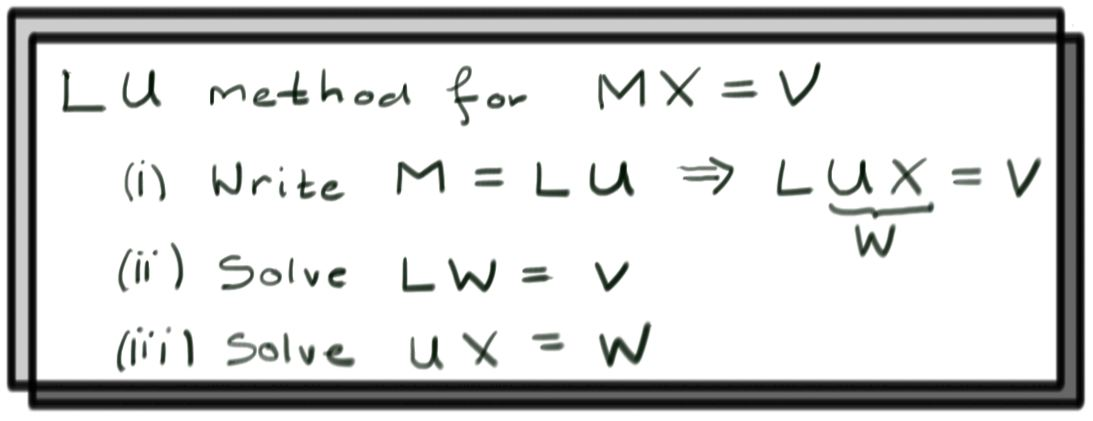
\includegraphics[scale=.3]{\luDecompPath/LU_solution.jpg}
\end{center}
%\end{figure}

\section{Finding an $LU$ Decomposition.}
\label{finding_LU_decomp}
 
For any given matrix, there are actually many different $LU$ decompositions.  However, there is a unique $LU$ decomposition in which the $L$ matrix has ones on the diagonal. In that case $L$ is called a \emph{lower unit triangular matrix}\index{Lower unit triangular matrix}.

To find the $LU$ decomposition, we'll create two sequences of matrices $L_0, L_1, \ldots$ and $U_0, U_1, \ldots$ such that at each step, $L_iU_i=M$.  Each of the $L_i$ will be lower triangular, but only the last $U_i$ will be upper triangular.

Start by setting $L_0=I$ and $U_0=M$, because $L_0U_0=M$. A main concept of this calculation is captured by the following example:

\begin{example}
Consider $$E=\begin{pmatrix}1&0\\\lambda&1\end{pmatrix}\, ,\qquad M=\begin{pmatrix}a&b&c&\cdots\\d&e&f&\cdots\end{pmatrix}\, .$$
Lets compute $EM$
$$
EM=\begin{pmatrix}a&b&c&\cdots\\d+\lambda a&e+\lambda b&f+\lambda c&\cdots\end{pmatrix}\, ,.
$$
Something neat happened here: multiplying $M$ by $E$ performed the row operation $R_2\to R_2+\lambda R-1$ on $M$.
Another interesting fact:
$$
E^{-1}:=\begin{pmatrix}1&0\\-\lambda&1\end{pmatrix}
$$ 
obeys (check this yourself...)
$$
E^{-1} E = 1\, .
$$
Hence $M=E^{-1} E M$ or, writing this out
$$
\begin{pmatrix}a&b&c&\cdots\\d&e&f&\cdots\end{pmatrix}=\begin{pmatrix}1&0\\-\lambda&1\end{pmatrix} \begin{pmatrix}a&b&c&\cdots\\d+\lambda a&e+\lambda b&f+\lambda c&\cdots\end{pmatrix}\, .
$$
Here the matrix on the left is lower triangular, while the matrix on the right has had a row operation performed on it.
\end{example}




\vspace{2mm}
We would like to  use the first row of $U_0$ to zero out the first entry of every row below it.  For our running example, $$U_0=M=\begin{pmatrix}
6 & 18 & 3 \\
2 & 12 & 1 \\
4 & 15 & 3 
\end{pmatrix}\, ,$$ so we would like to perform the row operations $R_2\to R_2 -\frac 13 R_1$ and $R_3\to R_3-\frac 23R_1$.
%so the second row minus $\frac{1}{3}$ of the first row will zero out the first entry in the second row.  Likewise, the third row minus $\frac{2}{3}$ of the first row will zero out the first entry in the third row.
If we perform these row operations on $U_0$ to produce 
$$U_1=\begin{pmatrix}
6 & 18 & 3 \\
0 & 6 & 0 \\
0 & 3 & 1 
\end{pmatrix}\, ,$$
we need to multiply this on the left by a lower triangular matrix $L_1$ so that the product $L_1U_1=M$ still.
The above example shows how to do this:
Set $L_1$ to be the lower triangular matrix whose first column is filled with the minus constants used to zero out the first column of $M$.  Then $$L_1 = \begin{pmatrix}
1 & 0 & 0 \\[1mm]
\frac{1}{3} & 1 & 0 \\[1mm]
\frac{2}{3} & 0 & 1 
\end{pmatrix}\, .$$  
%Set $U_1$ to be the matrix obtained by zeroing out the first column of $M$.  Then $U_1=\begin{pmatrix}
%6 & 18 & 3 \\
%0 & 6 & 0 \\
%0 & 3 & 1 
%\end{pmatrix}$.
By construction $L_1 U_1=M$, but you should compute this yourself as a double check.

Now repeat the process by zeroing the second column of $U_1$ below the diagonal using the second row of $U_1$ using the row operation
$R_3\to R_3-\frac 12 R_2$ to produce
$$U_2=\begin{pmatrix}6&18&3\\0&6&0\\0&0&1\end{pmatrix}\, .$$
The matrix that undoes this row operation is obtained in the same way we found $L_1$ above and is:
$$
\begin{pmatrix}
1&0&0\\
0&1&0\\
0&\frac 12& 0
\end{pmatrix}\, .
$$
Thus our answer for $L_2$ is the product of this matrix with $L_1$, namely
$$
L_2=
\begin{pmatrix}
1 & 0 & 0 \\[1mm]
\frac{1}{3} & 1 & 0 \\[1mm]
\frac{2}{3} & 0 & 1 
\end{pmatrix}\begin{pmatrix}
1&0&0\\
0&1&0\\
0&\frac 12& 0
\end{pmatrix}
=\begin{pmatrix}
1 & 0 & 0 \\[1mm]
\frac{1}{3} & 1 & 0 \\[1mm]
\frac{2}{3} & \frac{1}{2} & 1 
\end{pmatrix}\, .
$$
Notice that it is lower triangular because 

\begin{center}
\textcolor{brown}{THE PRODUCT OF LOWER TRIANGULAR MATRICES IS ALWAYS LOWER TRIANGULAR!}
\end{center}

\noindent
Moreover it is obtained by recording minus the constants used for all our row operations in the appropriate columns (this always works this way).
Moreover, $U_2$ is upper triangular and $M=L_2U_2$, we are done!
Putting this all together we have
$$M=\begin{pmatrix}
6 & 18 & 3 \\
2 & 12 & 1 \\
4 & 15 & 3 
\end{pmatrix}= \begin{pmatrix}
1 & 0 & 0 \\[1mm]
\frac{1}{3} & 1 & 0 \\[1mm]
\frac{2}{3} & \frac{1}{2} & 1 
\end{pmatrix}\begin{pmatrix}
6 & 18 & 3 \\
0 & 6 & 0 \\
0 & 0 & 1 
\end{pmatrix}\, .$$  
%Since $U_2$ is upper-triangular, we're done.  Inserting the new number into $L_1$ to get $L_2$ really is safe: the numbers in the first column don't affect the second column of $U_1$, since the first column of $U_1$ is already zeroed out.

If the matrix you're working with has more than three rows, just continue this process by zeroing out the next column below the diagonal, and repeat until there's nothing left to do.

\videoscriptlink{lu_decomposition_example.mp4}{Another $LU$ decomposition example}{scripts_lu_decomposition_example}

The fractions in the $L$ matrix are admittedly ugly.  For two matrices $LU$, we can multiply one entire column of $L$ by a constant $\lambda$ and divide the corresponding row of $U$ by the same constant without changing the product of the two matrices.  Then:

\begin{eqnarray*}
LU &=& \begin{pmatrix}
1 & 0 & 0 \\[1mm]
\frac{1}{3} & 1 & 0 \\[1mm]
\frac{2}{3} & \frac{1}{2} & 1 
\end{pmatrix}
I
\begin{pmatrix}
6 & 18 & 3 \\
0 & 6 & 0 \\
0 & 0 & 1 
\end{pmatrix} \\
&=&
\begin{pmatrix}
1 & 0 & 0 \\[1mm]
\frac{1}{3} & 1 & 0 \\[1mm]
\frac{2}{3} & \frac{1}{2} & 1 
\end{pmatrix}
\begin{pmatrix}
3 & 0 & 0 \\
0 & 6 & 0 \\
0 & 0 & 1 
\end{pmatrix}
\begin{pmatrix}
\frac{1}{3} & 0 & 0 \\[1mm]
0 & \frac{1}{6} & 0 \\[1mm]
0 & 0 & 1 
\end{pmatrix}
\begin{pmatrix}
6 & 18 & 3 \\
0 & 6 & 0 \\
0 & 0 & 1 
\end{pmatrix} \\
&=&
\begin{pmatrix}
3 & 0 & 0 \\
1 & 6 & 0 \\
2 & 3 & 1 
\end{pmatrix}\begin{pmatrix}
2 & 6 & 1 \\
0 & 1 & 0 \\
0 & 0 & 1 
\end{pmatrix}.
\end{eqnarray*}
The resulting matrix looks nicer, but isn't in standard (lower unit triangular matrix) form.

\reading{11}{2}
%\href{\webworkurl ReadingHomework11/2/}{Reading homework: problem 11.2}

For matrices that are not square, $LU$ decomposition still makes sense.  Given an $m\times n$ matrix $M$, for example we could write $M=LU$ with $L$ a square lower unit triangular matrix, and $U$ a rectangular matrix.  Then $L$ will be an $m\times m$ matrix, and $U$ will be an $m\times n$ matrix (of the same shape as $M$).  From here, the process is exactly the same as for a square matrix.  We create a sequence of matrices $L_i$ and $U_i$ that is eventually the $LU$ decomposition.  Again, we start with $L_0=I$ and $U_0=M$.

\begin{example}
Let's find the $LU$ decomposition of $M=U_0=\begin{pmatrix}
-2 & 1 & 3 \\
-4 & 4 & 1 
\end{pmatrix}$.  Since $M$ is a $2\times 3$ matrix, our decomposition will consist of a $2\times 2$ matrix and a $2\times 3$ matrix.  Then we start with $L_0=I_2=\begin{pmatrix}
1 & 0 \\
0 & 1
\end{pmatrix}$.

The next step is to zero-out the first column of $M$ below the diagonal.  There is only one row to cancel, then, and it can be removed by subtracting $2$ times the first row of $M$ to the second row of $M$.  Then:

\[
L_1=\begin{pmatrix}
1 & 0 \\
2 & 1
\end{pmatrix}, \qquad 
U_1 = \begin{pmatrix}
-2 & 1 & 3 \\
0 & 2 & -5 
\end{pmatrix}
\]
Since $U_1$ is upper triangular, we're done.  With a larger matrix, we would just continue the process.
\end{example}





\section{Block $LDU$ Decomposition}

Let $M$ be a square block matrix with square blocks $X,Y,Z,W$ such that $X^{-1}$ exists.  Then $M$ can be decomposed as a block $LDU$ decomposition, where $D$ is block diagonal, as follows:
\[
M=\begin{pmatrix}
X & Y \\
Z & W
\end{pmatrix}
\]

Then: \[M=\begin{pmatrix}
I &  0 \\
ZX^{-1} & I
\end{pmatrix}\begin{pmatrix}
X & 0 \\
0 & W-ZX^{-1}Y
\end{pmatrix}\begin{pmatrix}
I & X^{-1}Y \\
0 & I
\end{pmatrix}.\]
This can be checked explicitly simply by block-multiplying these three matrices.

\videoscriptlink{lu_decomposition_blocks.mp4}{Block $LDU$ Explanation}{scripts_lu_decomposition_blocks}

\begin{example}
For a $2\times 2$ matrix, we can regard each entry as a block.
\[
\begin{pmatrix}
1 & 2 \\
3 & 4
\end{pmatrix}=
\begin{pmatrix}
1 & 0 \\
3 & 1
\end{pmatrix}
\begin{pmatrix}
1 & 0 \\
0 & -2
\end{pmatrix}
\begin{pmatrix}
1 & 2 \\
0 & 1
\end{pmatrix}
\]
By multiplying the diagonal matrix by the upper triangular matrix, we get the standard $LU$ decomposition of the matrix.
\end{example}


%\section*{References}
%Wikipedia:
%\begin{itemize}
%\item \href{http://en.wikipedia.org/wiki/LU_decomposition}{$LU$ Decomposition}
%\item \href{http://en.wikipedia.org/wiki/Block_LU_decomposition}{Block $LU$ Decomposition}
%\end{itemize}

\section{Review Problems}



\begin{enumerate}

\item Let $D=\begin{pmatrix}
\lambda_1 & \mc0 \\
\mc0 & \lambda_2 \\
\end{pmatrix}$.
\begin{enumerate}
\item Write $D$ in terms of the vectors $e_1$ and $e_2$, and their transposes.
\item Suppose $P=\begin{pmatrix}
a & b \\
c & d \\
\end{pmatrix}$ is invertible.  Show that $D$ is similar to
\[
M=\frac{1}{ad-bc}\begin{pmatrix}
\lambda_1ad-\lambda_2bc & -(\lambda_1-\lambda_2)ab \\[1mm]
(\lambda_1-\lambda_2)cd & -\lambda_1bc + \lambda_2ad
\end{pmatrix}.
\]
\item Suppose the vectors $\rowvec{a,b}$ and $\rowvec{c,d}$ are orthogonal.  What can you say about $M$ in this case? (Hint: think about what \(M^T\) is equal to.)
\end{enumerate}

\phantomnewpage

\item \label{orthogprob} Suppose $S=\{v_1, \ldots, v_n \}$ is an \emph{orthogonal} (not orthonormal) basis for~$\Re^n$.  Then we can write any vector $v$ as $v=\sum_ic^iv_i$ for some constants $c^i$.  Find a formula for the constants $c^i$ in terms of $v$ and the vectors in~$S$.

\Videoscriptlink{orthonormal_bases_hint.mp4}{Hint}{scripts_orthonormal_bases_hint}
\phantomnewpage

\item \label{orthogprojprob} Let $u,v$ be linearly independent vectors in $\Re^3$, and $P=\spa \{ u,v\}$ be the plane spanned by $u$ and $v$.  
\begin{enumerate}
\item Is the vector $v^\bot := v-\frac{u\cdot v}{u\cdot u}u$ in the plane $P$?
\item  What is the (cosine of the) angle between $v^\bot$ and $u$?
\item %Given your solution to the above, 
How can you find a third vector perpendicular to both $u$ and $v^\bot$?
\item  Construct an orthonormal basis for $\Re^3$ from $u$ and $v$.
\item  Test your abstract formul\ae\ starting with 
\[
u=\rowvec{1 , 2 , 0} \text{ and } v=\rowvec{0 , 1 , 1}.
\]
\end{enumerate}

\Videoscriptlink{orthonormal_bases_hint3.mp4}{Hint}{scripts_orthonormal_bases_hint3}

\phantomnewpage



\item Find an orthonormal  basis for $\Re^4$ which includes $(1,1,1,1)$ using the following procedure:\\
\begin{enumerate} 
\item Pick a vector perpendicular to the vector 
$$v_1 =\colvec{1\\1\\1\\1}$$ from the solution set of the matrix equation $$v_1^Tx=0\, .$$ Pick the vector $v_2$ obtained from the standard Gaussian elimination procedure which is the coefficient of $x_2$.
\item Pick a vector perpendicular to both $v_1$ and $v_2$ from the solutions set of the matrix equation $$\colvec{v_1^T\\[1mm]v_2^T}x=0\, .$$ Pick the vector $v_3$ obtained from the standard Gaussian elimination procedure with $x_3$ as the coefficient. 
\item Pick a vector perpendicular to $v_1,v_2,$ and $v_3$ from the solution set of the matrix equation $$\colvec{v_1^T\\[1mm]v_2^T\\[1mm]v_3^T}x=0\, .$$  Pick the vector $v_4$ obtained from the standard Gaussian elimination procedure with $x_3$ as the coefficient. 
\item Normalize the four vectors obtained   above.
\end{enumerate}


\item Use the inner product $$f\cdot g := \int_0^1 f(x)g(x)dx$$  on the vector space $V={\rm span} \{1,x,x^2,x^3\}$ to perform the Gram-Schmidt procedure on the set of vectors $\{1,x,x^2,x^3\}$. 

\item Use the inner product $$f\cdot g := \int_0^{2\pi} f(x)g(x)dx$$  on the vector space $V={\rm span} \{\sin(x),\sin(2x),\sin(3x) \}$ to perform the Gram-Schmidt procedure on the set of vectors $\{\sin(x),\sin(2x),\sin(3x) \}$. \\
Try to build an orthonormal basis for the vector space $$\spa \{ \sin(nx)~| ~n\in \N \}\, .$$
%What do you suspect about the vector space $\spa \{ \sin(nx)~| ~n\in \N \}$?\\
%What do you suspect about the vector space $\spa \{ \sin(ax)~|~ a \in \Re \}$?
\item 
\begin{enumerate}
\item
Show that if $Q$ is an orthogonal $n\times n$ matrix, then $$u\dotprod v = (Qu)\dotprod (Qv)\, ,$$ for any $u,v\in \Re^n$. That is, $Q$ preserves the inner product. 
\item Does $Q$ preserve the outer product? 
\item  If the set of vectors $\{ u_1,\dots,u_n\}$ is orthonormal and $\{ \lambda_1,\cdots,\lambda_n\}$ is a set of numbers, 
then what are the eigenvalues and eigenvectors of the matrix
$M=\sum_{i=1}^n \lambda_i u_i u_i^T$? 
\item How would the eigenvectors and eigenvalues of this matrix change if we replaced  $\{ u_1,\dots,u_n\}$ by $\{ Qu_1,\dots,Q u_n\}$?
\end{enumerate}


\item Carefully write out the Gram-Schmidt procedure for the set of vectors 
$$\left\{ \colvec{1\\1\\1}, \colvec{1\\-1\\1}, \colvec{1\\1\\-1} \right\} \, .$$ Is it possible to rescale the second vector obtained in the procedure to a vector with integer components? 


\item 
\label{basisortho}
\begin{enumerate}
\item Suppose $u$ and $v$ are linearly independent.  Show that $u$ and $v^\perp$ are also linearly independent.  Explain why $\{u, v^\perp\}$ is a basis for $\spa \{u,v\}$.



\Videoscriptlink{gram_schmidt_and_orthogonal_complements_hint.mp4}{Hint}{gram_schmidt_and_orthogonal_complements_hint}

\item Repeat the previous problem, but with three independent vectors $u,v,w$
 where $v^\perp$ and $w^\perp$ are as defined by the Gram-Schmidt procedure. 
\end{enumerate}

\phantomnewpage


\item \label{QRprob} Find the $QR$ factorization of
$$
M=\begin{pmatrix}1&0&\phantom{\!-}2\\-1&2&0\\-1&-2&2
\end{pmatrix}\, .
$$

\phantomnewpage

\item Given any three vectors $u,v,w$, when do $v^\perp$ or $w^\perp$ of the Gram--Schmidt procedure vanish?

\phantomnewpage

\item For $U$ a subspace of $W$, use the subspace theorem to check that $U^\perp$ is a subspace of $W$.

\phantomnewpage


\phantomnewpage

\item %(Extra Credit) 
Let $S_n$ and $A_n$ define the space of $n \times n$ symmetric and anti-symmetric matrices, respectively. These are subspaces of the vector space $M^n_n$ of all $n\times n$ matrices. What is $\dim M^n_n$, $\dim S_n$, and $\dim A_n$? Show that $M^n_n = S_n + A_n$. Define an inner product on square matrices
$$
M\cdot N ={\rm tr} MN\, .
$$
Is $A_n^{\perp}=S_n$? Is $M^n_n = S_n \oplus A_n$?

%\emph{Hint: Note that $\dim S_n = \dim U_n$ where $U_n$ is the vector space of all $n \times n$ upper triangular matrices, and also note that $\dim A_n = \dim \widetilde{U}_n$ where $\widetilde{U}_n$ is the vector space of all strictly $n \times n$ upper triangular matrices (\emph{i.e.} the diagonal entries are all 0).}

\item The vector space $V={\rm span} \{ \sin(t),\sin(2t), \sin(3t) , \sin(3t)\}$ has an inner product: 
$$f\cdot g:=\int _0^{2\pi}f(t)g(t) dt\, .$$ Find the orthogonal compliment to $U={\rm span} \{ \sin(t)+\sin(2t) \}$ in $V$. Express $\sin(t)-\sin(2t)$ as  the sum of vectors from $U$ and $U^\perp$.

\end{enumerate}

\phantomnewpage

\newpage


\chapter{\luDecompTitle}
\label{LUdecomp}

Certain matrices are easier to work with than others.  In this section, we will see how to write any square\footnote{The case where $M$ is not square is dealt with at the end of the lecture.} matrix $M$ as the product of two simpler matrices.  We will write $$M=LU\, ,$$ where:
\begin{itemize}
\item $L$ is \emph{lower triangular}\index{Lower triangular matrix}.  This means that all entries above the main diagonal are zero.  In notation,
$L=(l^i_j)$ with $l^i_j=0$ for all $j>i$.
\[L=\begin{pmatrix}
l^1_1 & 0 & 0 & \cdots \\
l^2_1 & l^2_2 & 0 & \cdots \\
l^3_1 & l^3_2 & l^3_3 & \cdots \\
\vdots & \vdots & \vdots & \ddots \\
\end{pmatrix}
\]

\item $U$ is \emph{upper triangular}\index{Upper triangular matrix}.  This means that all entries below the main diagonal are zero.  In notation,
$U=(u^i_j)$ with $u^i_j=0$ for all $j<i$.
\[U=\begin{pmatrix}
u^1_1 & u^1_2 & u^1_3 & \cdots \\
0 & u^2_2 & u^2_3 & \cdots \\
0 & 0 & u^3_3 & \cdots \\
\vdots & \vdots & \vdots & \ddots \\
\end{pmatrix}
\]
\end{itemize}
$M=LU$ is called an \emph{$LU$ decomposition}\index{LU@$LU$ decomposition} of $M$.

This is a useful trick for  computational reasons; it is much easier to compute the inverse of an upper or lower triangular matrix than general matrices.  Since inverses are useful for solving linear systems, this makes solving any linear system associated to the matrix much faster as well.  The determinant---a very important quantity associated with any square matrix---is very easy to compute for triangular matrices.

\begin{example}
Linear systems associated to upper triangular matrices are very easy to solve by back substitution.
\[
\begin{amatrix}{2}
a & b & 1 \\
0 & c & e \\
\end{amatrix} \ \Rightarrow \ y=\frac{e}{c}\, , \quad x=\frac{1}{a}\left(1-\frac{be}{c}\right)
\]

\[
\begin{amatrix}{3}
1 & 0 & 0 & d \\
a & 1 & 0 & e \\
b & c & 1 & f \\
\end{amatrix} \Rightarrow x=d\, , \qquad y=e-ad\, , \qquad z=f-bd-c(e-ad)
\]
For lower triangular matrices, \emph{back} substitution\index{Back substitution} gives a quick solution; for upper triangular matrices, \emph{forward} substitution\index{Forward substitution} gives the solution.
\end{example}





\section{Using $LU$ Decomposition to Solve Linear Systems}

Suppose we have $M=LU$ and want to solve the system
\[
MX=LUX=V.
\]

\begin{itemize}
\item{Step 1:} Set $W=\colvec{u\\v\\w}=UX$.  

\item{Step 2:} Solve the system $LW=V$.  This should be simple by forward substitution since $L$ is lower triangular.  Suppose the solution to $LW=V$ is $W_0$.  

\item{Step 3:} Now solve the system $UX=W_0$.  This should be easy by backward substitution, since $U$ is upper triangular.  The solution to this system is the solution to the original system.
\end{itemize}
We can think of this as using the matrix $L$ to perform row operations on the matrix $U$ in order to solve the system; this idea also appears in the  study of determinants.

%\href{\webworkurl ReadingHomework11/1/}{Reading homework: problem 11.1}
\reading{11}{1}

\begin{example}
Consider the linear system:
\[
      \begin{linsys}{4}
            6x & +&18y & +&3z         &=& 3  \\[1mm]
            2x & +&12y & +&z	    &=& 19 \\[1mm]
            4x & +&15y & +&3z         &=& 0  
      \end{linsys}
\]

An $LU$ decomposition for the associated matrix $M$ is:
\[
\begin{pmatrix}
6 & 18 & 3 \\
2 & 12 & 1 \\
4 & 15 & 3 
\end{pmatrix} =
\begin{pmatrix}
3 & 0 & 0 \\
1 & 6 & 0 \\
2 & 3 & 1 
\end{pmatrix}
\begin{pmatrix}
2 & 6 & 1 \\
0 & 1 & 0 \\
0 & 0 & 1 
\end{pmatrix}.
\]

\begin{itemize}
\item{Step 1:} \hypertarget{LUproc}{Set} $W=\colvec{u\\v\\w}=UX$.  

\item{Step 2:} Solve the system $LW=V$:

\[
\begin{pmatrix}
3 & 0 & 0 \\
1 & 6 & 0 \\
2 & 3 & 1 
\end{pmatrix}
\colvec{u\\v\\w} =
\colvec{3\\19\\0}
\]

By substitution, we get $u=1$, $v=3$, and $w=-11$.  Then 
\[W_0=\colvec{1\\3\\-11}\]

\item{Step 3:} Solve the system $UX=W_0$.  
\[
\begin{pmatrix}
2 & 6 & 1 \\
0 & 1 & 0 \\
0 & 0 & 1 
\end{pmatrix}
\colvec{x\\y\\z} =
\colvec{1\\3\\-11}
\]
Back substitution gives $z=-11, y=3$, and $x=-3$.  

Then $X=\colvec{-3\\3\\-11}$, and we're done.
\end{itemize}
\end{example}

\videoscriptlink{lu_decomposition_using_lu_decomp.mp4}{Using a $LU$ decomposition}{scripts_lu_decomposition_using_lu_example}

%\begin{figure}
\begin{center}
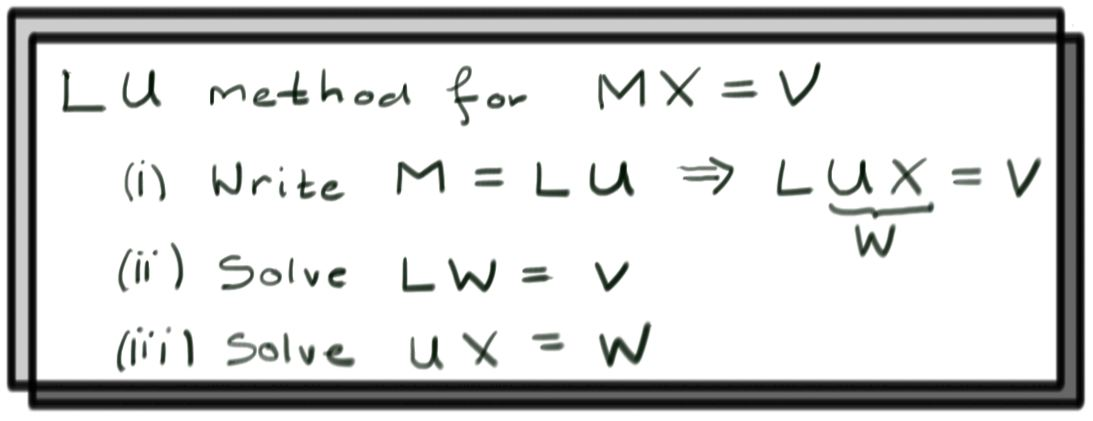
\includegraphics[scale=.3]{\luDecompPath/LU_solution.jpg}
\end{center}
%\end{figure}

\section{Finding an $LU$ Decomposition.}
\label{finding_LU_decomp}
 
For any given matrix, there are actually many different $LU$ decompositions.  However, there is a unique $LU$ decomposition in which the $L$ matrix has ones on the diagonal. In that case $L$ is called a \emph{lower unit triangular matrix}\index{Lower unit triangular matrix}.

To find the $LU$ decomposition, we'll create two sequences of matrices $L_0, L_1, \ldots$ and $U_0, U_1, \ldots$ such that at each step, $L_iU_i=M$.  Each of the $L_i$ will be lower triangular, but only the last $U_i$ will be upper triangular.

Start by setting $L_0=I$ and $U_0=M$, because $L_0U_0=M$. A main concept of this calculation is captured by the following example:

\begin{example}
Consider $$E=\begin{pmatrix}1&0\\\lambda&1\end{pmatrix}\, ,\qquad M=\begin{pmatrix}a&b&c&\cdots\\d&e&f&\cdots\end{pmatrix}\, .$$
Lets compute $EM$
$$
EM=\begin{pmatrix}a&b&c&\cdots\\d+\lambda a&e+\lambda b&f+\lambda c&\cdots\end{pmatrix}\, ,.
$$
Something neat happened here: multiplying $M$ by $E$ performed the row operation $R_2\to R_2+\lambda R-1$ on $M$.
Another interesting fact:
$$
E^{-1}:=\begin{pmatrix}1&0\\-\lambda&1\end{pmatrix}
$$ 
obeys (check this yourself...)
$$
E^{-1} E = 1\, .
$$
Hence $M=E^{-1} E M$ or, writing this out
$$
\begin{pmatrix}a&b&c&\cdots\\d&e&f&\cdots\end{pmatrix}=\begin{pmatrix}1&0\\-\lambda&1\end{pmatrix} \begin{pmatrix}a&b&c&\cdots\\d+\lambda a&e+\lambda b&f+\lambda c&\cdots\end{pmatrix}\, .
$$
Here the matrix on the left is lower triangular, while the matrix on the right has had a row operation performed on it.
\end{example}




\vspace{2mm}
We would like to  use the first row of $U_0$ to zero out the first entry of every row below it.  For our running example, $$U_0=M=\begin{pmatrix}
6 & 18 & 3 \\
2 & 12 & 1 \\
4 & 15 & 3 
\end{pmatrix}\, ,$$ so we would like to perform the row operations $R_2\to R_2 -\frac 13 R_1$ and $R_3\to R_3-\frac 23R_1$.
%so the second row minus $\frac{1}{3}$ of the first row will zero out the first entry in the second row.  Likewise, the third row minus $\frac{2}{3}$ of the first row will zero out the first entry in the third row.
If we perform these row operations on $U_0$ to produce 
$$U_1=\begin{pmatrix}
6 & 18 & 3 \\
0 & 6 & 0 \\
0 & 3 & 1 
\end{pmatrix}\, ,$$
we need to multiply this on the left by a lower triangular matrix $L_1$ so that the product $L_1U_1=M$ still.
The above example shows how to do this:
Set $L_1$ to be the lower triangular matrix whose first column is filled with the minus constants used to zero out the first column of $M$.  Then $$L_1 = \begin{pmatrix}
1 & 0 & 0 \\[1mm]
\frac{1}{3} & 1 & 0 \\[1mm]
\frac{2}{3} & 0 & 1 
\end{pmatrix}\, .$$  
%Set $U_1$ to be the matrix obtained by zeroing out the first column of $M$.  Then $U_1=\begin{pmatrix}
%6 & 18 & 3 \\
%0 & 6 & 0 \\
%0 & 3 & 1 
%\end{pmatrix}$.
By construction $L_1 U_1=M$, but you should compute this yourself as a double check.

Now repeat the process by zeroing the second column of $U_1$ below the diagonal using the second row of $U_1$ using the row operation
$R_3\to R_3-\frac 12 R_2$ to produce
$$U_2=\begin{pmatrix}6&18&3\\0&6&0\\0&0&1\end{pmatrix}\, .$$
The matrix that undoes this row operation is obtained in the same way we found $L_1$ above and is:
$$
\begin{pmatrix}
1&0&0\\
0&1&0\\
0&\frac 12& 0
\end{pmatrix}\, .
$$
Thus our answer for $L_2$ is the product of this matrix with $L_1$, namely
$$
L_2=
\begin{pmatrix}
1 & 0 & 0 \\[1mm]
\frac{1}{3} & 1 & 0 \\[1mm]
\frac{2}{3} & 0 & 1 
\end{pmatrix}\begin{pmatrix}
1&0&0\\
0&1&0\\
0&\frac 12& 0
\end{pmatrix}
=\begin{pmatrix}
1 & 0 & 0 \\[1mm]
\frac{1}{3} & 1 & 0 \\[1mm]
\frac{2}{3} & \frac{1}{2} & 1 
\end{pmatrix}\, .
$$
Notice that it is lower triangular because 

\begin{center}
\textcolor{brown}{THE PRODUCT OF LOWER TRIANGULAR MATRICES IS ALWAYS LOWER TRIANGULAR!}
\end{center}

\noindent
Moreover it is obtained by recording minus the constants used for all our row operations in the appropriate columns (this always works this way).
Moreover, $U_2$ is upper triangular and $M=L_2U_2$, we are done!
Putting this all together we have
$$M=\begin{pmatrix}
6 & 18 & 3 \\
2 & 12 & 1 \\
4 & 15 & 3 
\end{pmatrix}= \begin{pmatrix}
1 & 0 & 0 \\[1mm]
\frac{1}{3} & 1 & 0 \\[1mm]
\frac{2}{3} & \frac{1}{2} & 1 
\end{pmatrix}\begin{pmatrix}
6 & 18 & 3 \\
0 & 6 & 0 \\
0 & 0 & 1 
\end{pmatrix}\, .$$  
%Since $U_2$ is upper-triangular, we're done.  Inserting the new number into $L_1$ to get $L_2$ really is safe: the numbers in the first column don't affect the second column of $U_1$, since the first column of $U_1$ is already zeroed out.

If the matrix you're working with has more than three rows, just continue this process by zeroing out the next column below the diagonal, and repeat until there's nothing left to do.

\videoscriptlink{lu_decomposition_example.mp4}{Another $LU$ decomposition example}{scripts_lu_decomposition_example}

The fractions in the $L$ matrix are admittedly ugly.  For two matrices $LU$, we can multiply one entire column of $L$ by a constant $\lambda$ and divide the corresponding row of $U$ by the same constant without changing the product of the two matrices.  Then:

\begin{eqnarray*}
LU &=& \begin{pmatrix}
1 & 0 & 0 \\[1mm]
\frac{1}{3} & 1 & 0 \\[1mm]
\frac{2}{3} & \frac{1}{2} & 1 
\end{pmatrix}
I
\begin{pmatrix}
6 & 18 & 3 \\
0 & 6 & 0 \\
0 & 0 & 1 
\end{pmatrix} \\
&=&
\begin{pmatrix}
1 & 0 & 0 \\[1mm]
\frac{1}{3} & 1 & 0 \\[1mm]
\frac{2}{3} & \frac{1}{2} & 1 
\end{pmatrix}
\begin{pmatrix}
3 & 0 & 0 \\
0 & 6 & 0 \\
0 & 0 & 1 
\end{pmatrix}
\begin{pmatrix}
\frac{1}{3} & 0 & 0 \\[1mm]
0 & \frac{1}{6} & 0 \\[1mm]
0 & 0 & 1 
\end{pmatrix}
\begin{pmatrix}
6 & 18 & 3 \\
0 & 6 & 0 \\
0 & 0 & 1 
\end{pmatrix} \\
&=&
\begin{pmatrix}
3 & 0 & 0 \\
1 & 6 & 0 \\
2 & 3 & 1 
\end{pmatrix}\begin{pmatrix}
2 & 6 & 1 \\
0 & 1 & 0 \\
0 & 0 & 1 
\end{pmatrix}.
\end{eqnarray*}
The resulting matrix looks nicer, but isn't in standard (lower unit triangular matrix) form.

\reading{11}{2}
%\href{\webworkurl ReadingHomework11/2/}{Reading homework: problem 11.2}

For matrices that are not square, $LU$ decomposition still makes sense.  Given an $m\times n$ matrix $M$, for example we could write $M=LU$ with $L$ a square lower unit triangular matrix, and $U$ a rectangular matrix.  Then $L$ will be an $m\times m$ matrix, and $U$ will be an $m\times n$ matrix (of the same shape as $M$).  From here, the process is exactly the same as for a square matrix.  We create a sequence of matrices $L_i$ and $U_i$ that is eventually the $LU$ decomposition.  Again, we start with $L_0=I$ and $U_0=M$.

\begin{example}
Let's find the $LU$ decomposition of $M=U_0=\begin{pmatrix}
-2 & 1 & 3 \\
-4 & 4 & 1 
\end{pmatrix}$.  Since $M$ is a $2\times 3$ matrix, our decomposition will consist of a $2\times 2$ matrix and a $2\times 3$ matrix.  Then we start with $L_0=I_2=\begin{pmatrix}
1 & 0 \\
0 & 1
\end{pmatrix}$.

The next step is to zero-out the first column of $M$ below the diagonal.  There is only one row to cancel, then, and it can be removed by subtracting $2$ times the first row of $M$ to the second row of $M$.  Then:

\[
L_1=\begin{pmatrix}
1 & 0 \\
2 & 1
\end{pmatrix}, \qquad 
U_1 = \begin{pmatrix}
-2 & 1 & 3 \\
0 & 2 & -5 
\end{pmatrix}
\]
Since $U_1$ is upper triangular, we're done.  With a larger matrix, we would just continue the process.
\end{example}





\section{Block $LDU$ Decomposition}

Let $M$ be a square block matrix with square blocks $X,Y,Z,W$ such that $X^{-1}$ exists.  Then $M$ can be decomposed as a block $LDU$ decomposition, where $D$ is block diagonal, as follows:
\[
M=\begin{pmatrix}
X & Y \\
Z & W
\end{pmatrix}
\]

Then: \[M=\begin{pmatrix}
I &  0 \\
ZX^{-1} & I
\end{pmatrix}\begin{pmatrix}
X & 0 \\
0 & W-ZX^{-1}Y
\end{pmatrix}\begin{pmatrix}
I & X^{-1}Y \\
0 & I
\end{pmatrix}.\]
This can be checked explicitly simply by block-multiplying these three matrices.

\videoscriptlink{lu_decomposition_blocks.mp4}{Block $LDU$ Explanation}{scripts_lu_decomposition_blocks}

\begin{example}
For a $2\times 2$ matrix, we can regard each entry as a block.
\[
\begin{pmatrix}
1 & 2 \\
3 & 4
\end{pmatrix}=
\begin{pmatrix}
1 & 0 \\
3 & 1
\end{pmatrix}
\begin{pmatrix}
1 & 0 \\
0 & -2
\end{pmatrix}
\begin{pmatrix}
1 & 2 \\
0 & 1
\end{pmatrix}
\]
By multiplying the diagonal matrix by the upper triangular matrix, we get the standard $LU$ decomposition of the matrix.
\end{example}


%\section*{References}
%Wikipedia:
%\begin{itemize}
%\item \href{http://en.wikipedia.org/wiki/LU_decomposition}{$LU$ Decomposition}
%\item \href{http://en.wikipedia.org/wiki/Block_LU_decomposition}{Block $LU$ Decomposition}
%\end{itemize}

\section{Review Problems}



\begin{enumerate}

\item Let $D=\begin{pmatrix}
\lambda_1 & \mc0 \\
\mc0 & \lambda_2 \\
\end{pmatrix}$.
\begin{enumerate}
\item Write $D$ in terms of the vectors $e_1$ and $e_2$, and their transposes.
\item Suppose $P=\begin{pmatrix}
a & b \\
c & d \\
\end{pmatrix}$ is invertible.  Show that $D$ is similar to
\[
M=\frac{1}{ad-bc}\begin{pmatrix}
\lambda_1ad-\lambda_2bc & -(\lambda_1-\lambda_2)ab \\[1mm]
(\lambda_1-\lambda_2)cd & -\lambda_1bc + \lambda_2ad
\end{pmatrix}.
\]
\item Suppose the vectors $\rowvec{a,b}$ and $\rowvec{c,d}$ are orthogonal.  What can you say about $M$ in this case? (Hint: think about what \(M^T\) is equal to.)
\end{enumerate}

\phantomnewpage

\item \label{orthogprob} Suppose $S=\{v_1, \ldots, v_n \}$ is an \emph{orthogonal} (not orthonormal) basis for~$\Re^n$.  Then we can write any vector $v$ as $v=\sum_ic^iv_i$ for some constants $c^i$.  Find a formula for the constants $c^i$ in terms of $v$ and the vectors in~$S$.

\Videoscriptlink{orthonormal_bases_hint.mp4}{Hint}{scripts_orthonormal_bases_hint}
\phantomnewpage

\item \label{orthogprojprob} Let $u,v$ be linearly independent vectors in $\Re^3$, and $P=\spa \{ u,v\}$ be the plane spanned by $u$ and $v$.  
\begin{enumerate}
\item Is the vector $v^\bot := v-\frac{u\cdot v}{u\cdot u}u$ in the plane $P$?
\item  What is the (cosine of the) angle between $v^\bot$ and $u$?
\item %Given your solution to the above, 
How can you find a third vector perpendicular to both $u$ and $v^\bot$?
\item  Construct an orthonormal basis for $\Re^3$ from $u$ and $v$.
\item  Test your abstract formul\ae\ starting with 
\[
u=\rowvec{1 , 2 , 0} \text{ and } v=\rowvec{0 , 1 , 1}.
\]
\end{enumerate}

\Videoscriptlink{orthonormal_bases_hint3.mp4}{Hint}{scripts_orthonormal_bases_hint3}

\phantomnewpage



\item Find an orthonormal  basis for $\Re^4$ which includes $(1,1,1,1)$ using the following procedure:\\
\begin{enumerate} 
\item Pick a vector perpendicular to the vector 
$$v_1 =\colvec{1\\1\\1\\1}$$ from the solution set of the matrix equation $$v_1^Tx=0\, .$$ Pick the vector $v_2$ obtained from the standard Gaussian elimination procedure which is the coefficient of $x_2$.
\item Pick a vector perpendicular to both $v_1$ and $v_2$ from the solutions set of the matrix equation $$\colvec{v_1^T\\[1mm]v_2^T}x=0\, .$$ Pick the vector $v_3$ obtained from the standard Gaussian elimination procedure with $x_3$ as the coefficient. 
\item Pick a vector perpendicular to $v_1,v_2,$ and $v_3$ from the solution set of the matrix equation $$\colvec{v_1^T\\[1mm]v_2^T\\[1mm]v_3^T}x=0\, .$$  Pick the vector $v_4$ obtained from the standard Gaussian elimination procedure with $x_3$ as the coefficient. 
\item Normalize the four vectors obtained   above.
\end{enumerate}


\item Use the inner product $$f\cdot g := \int_0^1 f(x)g(x)dx$$  on the vector space $V={\rm span} \{1,x,x^2,x^3\}$ to perform the Gram-Schmidt procedure on the set of vectors $\{1,x,x^2,x^3\}$. 

\item Use the inner product $$f\cdot g := \int_0^{2\pi} f(x)g(x)dx$$  on the vector space $V={\rm span} \{\sin(x),\sin(2x),\sin(3x) \}$ to perform the Gram-Schmidt procedure on the set of vectors $\{\sin(x),\sin(2x),\sin(3x) \}$. \\
Try to build an orthonormal basis for the vector space $$\spa \{ \sin(nx)~| ~n\in \N \}\, .$$
%What do you suspect about the vector space $\spa \{ \sin(nx)~| ~n\in \N \}$?\\
%What do you suspect about the vector space $\spa \{ \sin(ax)~|~ a \in \Re \}$?
\item 
\begin{enumerate}
\item
Show that if $Q$ is an orthogonal $n\times n$ matrix, then $$u\dotprod v = (Qu)\dotprod (Qv)\, ,$$ for any $u,v\in \Re^n$. That is, $Q$ preserves the inner product. 
\item Does $Q$ preserve the outer product? 
\item  If the set of vectors $\{ u_1,\dots,u_n\}$ is orthonormal and $\{ \lambda_1,\cdots,\lambda_n\}$ is a set of numbers, 
then what are the eigenvalues and eigenvectors of the matrix
$M=\sum_{i=1}^n \lambda_i u_i u_i^T$? 
\item How would the eigenvectors and eigenvalues of this matrix change if we replaced  $\{ u_1,\dots,u_n\}$ by $\{ Qu_1,\dots,Q u_n\}$?
\end{enumerate}


\item Carefully write out the Gram-Schmidt procedure for the set of vectors 
$$\left\{ \colvec{1\\1\\1}, \colvec{1\\-1\\1}, \colvec{1\\1\\-1} \right\} \, .$$ Is it possible to rescale the second vector obtained in the procedure to a vector with integer components? 


\item 
\label{basisortho}
\begin{enumerate}
\item Suppose $u$ and $v$ are linearly independent.  Show that $u$ and $v^\perp$ are also linearly independent.  Explain why $\{u, v^\perp\}$ is a basis for $\spa \{u,v\}$.



\Videoscriptlink{gram_schmidt_and_orthogonal_complements_hint.mp4}{Hint}{gram_schmidt_and_orthogonal_complements_hint}

\item Repeat the previous problem, but with three independent vectors $u,v,w$
 where $v^\perp$ and $w^\perp$ are as defined by the Gram-Schmidt procedure. 
\end{enumerate}

\phantomnewpage


\item \label{QRprob} Find the $QR$ factorization of
$$
M=\begin{pmatrix}1&0&\phantom{\!-}2\\-1&2&0\\-1&-2&2
\end{pmatrix}\, .
$$

\phantomnewpage

\item Given any three vectors $u,v,w$, when do $v^\perp$ or $w^\perp$ of the Gram--Schmidt procedure vanish?

\phantomnewpage

\item For $U$ a subspace of $W$, use the subspace theorem to check that $U^\perp$ is a subspace of $W$.

\phantomnewpage


\phantomnewpage

\item %(Extra Credit) 
Let $S_n$ and $A_n$ define the space of $n \times n$ symmetric and anti-symmetric matrices, respectively. These are subspaces of the vector space $M^n_n$ of all $n\times n$ matrices. What is $\dim M^n_n$, $\dim S_n$, and $\dim A_n$? Show that $M^n_n = S_n + A_n$. Define an inner product on square matrices
$$
M\cdot N ={\rm tr} MN\, .
$$
Is $A_n^{\perp}=S_n$? Is $M^n_n = S_n \oplus A_n$?

%\emph{Hint: Note that $\dim S_n = \dim U_n$ where $U_n$ is the vector space of all $n \times n$ upper triangular matrices, and also note that $\dim A_n = \dim \widetilde{U}_n$ where $\widetilde{U}_n$ is the vector space of all strictly $n \times n$ upper triangular matrices (\emph{i.e.} the diagonal entries are all 0).}

\item The vector space $V={\rm span} \{ \sin(t),\sin(2t), \sin(3t) , \sin(3t)\}$ has an inner product: 
$$f\cdot g:=\int _0^{2\pi}f(t)g(t) dt\, .$$ Find the orthogonal compliment to $U={\rm span} \{ \sin(t)+\sin(2t) \}$ in $V$. Express $\sin(t)-\sin(2t)$ as  the sum of vectors from $U$ and $U^\perp$.

\end{enumerate}

\phantomnewpage

\newpage
 

\chapter{\luDecompTitle}
\label{LUdecomp}

Certain matrices are easier to work with than others.  In this section, we will see how to write any square\footnote{The case where $M$ is not square is dealt with at the end of the lecture.} matrix $M$ as the product of two simpler matrices.  We will write $$M=LU\, ,$$ where:
\begin{itemize}
\item $L$ is \emph{lower triangular}\index{Lower triangular matrix}.  This means that all entries above the main diagonal are zero.  In notation,
$L=(l^i_j)$ with $l^i_j=0$ for all $j>i$.
\[L=\begin{pmatrix}
l^1_1 & 0 & 0 & \cdots \\
l^2_1 & l^2_2 & 0 & \cdots \\
l^3_1 & l^3_2 & l^3_3 & \cdots \\
\vdots & \vdots & \vdots & \ddots \\
\end{pmatrix}
\]

\item $U$ is \emph{upper triangular}\index{Upper triangular matrix}.  This means that all entries below the main diagonal are zero.  In notation,
$U=(u^i_j)$ with $u^i_j=0$ for all $j<i$.
\[U=\begin{pmatrix}
u^1_1 & u^1_2 & u^1_3 & \cdots \\
0 & u^2_2 & u^2_3 & \cdots \\
0 & 0 & u^3_3 & \cdots \\
\vdots & \vdots & \vdots & \ddots \\
\end{pmatrix}
\]
\end{itemize}
$M=LU$ is called an \emph{$LU$ decomposition}\index{LU@$LU$ decomposition} of $M$.

This is a useful trick for  computational reasons; it is much easier to compute the inverse of an upper or lower triangular matrix than general matrices.  Since inverses are useful for solving linear systems, this makes solving any linear system associated to the matrix much faster as well.  The determinant---a very important quantity associated with any square matrix---is very easy to compute for triangular matrices.

\begin{example}
Linear systems associated to upper triangular matrices are very easy to solve by back substitution.
\[
\begin{amatrix}{2}
a & b & 1 \\
0 & c & e \\
\end{amatrix} \ \Rightarrow \ y=\frac{e}{c}\, , \quad x=\frac{1}{a}\left(1-\frac{be}{c}\right)
\]

\[
\begin{amatrix}{3}
1 & 0 & 0 & d \\
a & 1 & 0 & e \\
b & c & 1 & f \\
\end{amatrix} \Rightarrow x=d\, , \qquad y=e-ad\, , \qquad z=f-bd-c(e-ad)
\]
For lower triangular matrices, \emph{back} substitution\index{Back substitution} gives a quick solution; for upper triangular matrices, \emph{forward} substitution\index{Forward substitution} gives the solution.
\end{example}





\section{Using $LU$ Decomposition to Solve Linear Systems}

Suppose we have $M=LU$ and want to solve the system
\[
MX=LUX=V.
\]

\begin{itemize}
\item{Step 1:} Set $W=\colvec{u\\v\\w}=UX$.  

\item{Step 2:} Solve the system $LW=V$.  This should be simple by forward substitution since $L$ is lower triangular.  Suppose the solution to $LW=V$ is $W_0$.  

\item{Step 3:} Now solve the system $UX=W_0$.  This should be easy by backward substitution, since $U$ is upper triangular.  The solution to this system is the solution to the original system.
\end{itemize}
We can think of this as using the matrix $L$ to perform row operations on the matrix $U$ in order to solve the system; this idea also appears in the  study of determinants.

%\href{\webworkurl ReadingHomework11/1/}{Reading homework: problem 11.1}
\reading{11}{1}

\begin{example}
Consider the linear system:
\[
      \begin{linsys}{4}
            6x & +&18y & +&3z         &=& 3  \\[1mm]
            2x & +&12y & +&z	    &=& 19 \\[1mm]
            4x & +&15y & +&3z         &=& 0  
      \end{linsys}
\]

An $LU$ decomposition for the associated matrix $M$ is:
\[
\begin{pmatrix}
6 & 18 & 3 \\
2 & 12 & 1 \\
4 & 15 & 3 
\end{pmatrix} =
\begin{pmatrix}
3 & 0 & 0 \\
1 & 6 & 0 \\
2 & 3 & 1 
\end{pmatrix}
\begin{pmatrix}
2 & 6 & 1 \\
0 & 1 & 0 \\
0 & 0 & 1 
\end{pmatrix}.
\]

\begin{itemize}
\item{Step 1:} \hypertarget{LUproc}{Set} $W=\colvec{u\\v\\w}=UX$.  

\item{Step 2:} Solve the system $LW=V$:

\[
\begin{pmatrix}
3 & 0 & 0 \\
1 & 6 & 0 \\
2 & 3 & 1 
\end{pmatrix}
\colvec{u\\v\\w} =
\colvec{3\\19\\0}
\]

By substitution, we get $u=1$, $v=3$, and $w=-11$.  Then 
\[W_0=\colvec{1\\3\\-11}\]

\item{Step 3:} Solve the system $UX=W_0$.  
\[
\begin{pmatrix}
2 & 6 & 1 \\
0 & 1 & 0 \\
0 & 0 & 1 
\end{pmatrix}
\colvec{x\\y\\z} =
\colvec{1\\3\\-11}
\]
Back substitution gives $z=-11, y=3$, and $x=-3$.  

Then $X=\colvec{-3\\3\\-11}$, and we're done.
\end{itemize}
\end{example}

\videoscriptlink{lu_decomposition_using_lu_decomp.mp4}{Using a $LU$ decomposition}{scripts_lu_decomposition_using_lu_example}

%\begin{figure}
\begin{center}
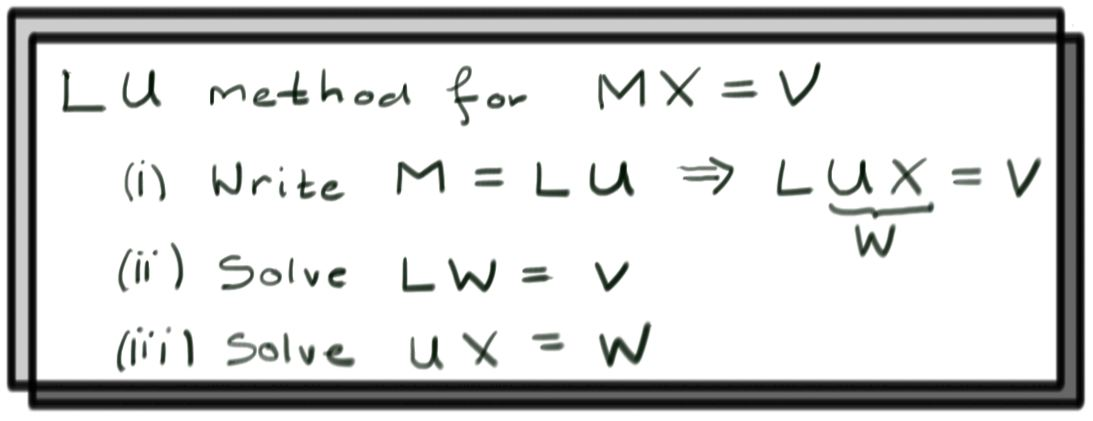
\includegraphics[scale=.3]{\luDecompPath/LU_solution.jpg}
\end{center}
%\end{figure}

\section{Finding an $LU$ Decomposition.}
\label{finding_LU_decomp}
 
For any given matrix, there are actually many different $LU$ decompositions.  However, there is a unique $LU$ decomposition in which the $L$ matrix has ones on the diagonal. In that case $L$ is called a \emph{lower unit triangular matrix}\index{Lower unit triangular matrix}.

To find the $LU$ decomposition, we'll create two sequences of matrices $L_0, L_1, \ldots$ and $U_0, U_1, \ldots$ such that at each step, $L_iU_i=M$.  Each of the $L_i$ will be lower triangular, but only the last $U_i$ will be upper triangular.

Start by setting $L_0=I$ and $U_0=M$, because $L_0U_0=M$. A main concept of this calculation is captured by the following example:

\begin{example}
Consider $$E=\begin{pmatrix}1&0\\\lambda&1\end{pmatrix}\, ,\qquad M=\begin{pmatrix}a&b&c&\cdots\\d&e&f&\cdots\end{pmatrix}\, .$$
Lets compute $EM$
$$
EM=\begin{pmatrix}a&b&c&\cdots\\d+\lambda a&e+\lambda b&f+\lambda c&\cdots\end{pmatrix}\, ,.
$$
Something neat happened here: multiplying $M$ by $E$ performed the row operation $R_2\to R_2+\lambda R-1$ on $M$.
Another interesting fact:
$$
E^{-1}:=\begin{pmatrix}1&0\\-\lambda&1\end{pmatrix}
$$ 
obeys (check this yourself...)
$$
E^{-1} E = 1\, .
$$
Hence $M=E^{-1} E M$ or, writing this out
$$
\begin{pmatrix}a&b&c&\cdots\\d&e&f&\cdots\end{pmatrix}=\begin{pmatrix}1&0\\-\lambda&1\end{pmatrix} \begin{pmatrix}a&b&c&\cdots\\d+\lambda a&e+\lambda b&f+\lambda c&\cdots\end{pmatrix}\, .
$$
Here the matrix on the left is lower triangular, while the matrix on the right has had a row operation performed on it.
\end{example}




\vspace{2mm}
We would like to  use the first row of $U_0$ to zero out the first entry of every row below it.  For our running example, $$U_0=M=\begin{pmatrix}
6 & 18 & 3 \\
2 & 12 & 1 \\
4 & 15 & 3 
\end{pmatrix}\, ,$$ so we would like to perform the row operations $R_2\to R_2 -\frac 13 R_1$ and $R_3\to R_3-\frac 23R_1$.
%so the second row minus $\frac{1}{3}$ of the first row will zero out the first entry in the second row.  Likewise, the third row minus $\frac{2}{3}$ of the first row will zero out the first entry in the third row.
If we perform these row operations on $U_0$ to produce 
$$U_1=\begin{pmatrix}
6 & 18 & 3 \\
0 & 6 & 0 \\
0 & 3 & 1 
\end{pmatrix}\, ,$$
we need to multiply this on the left by a lower triangular matrix $L_1$ so that the product $L_1U_1=M$ still.
The above example shows how to do this:
Set $L_1$ to be the lower triangular matrix whose first column is filled with the minus constants used to zero out the first column of $M$.  Then $$L_1 = \begin{pmatrix}
1 & 0 & 0 \\[1mm]
\frac{1}{3} & 1 & 0 \\[1mm]
\frac{2}{3} & 0 & 1 
\end{pmatrix}\, .$$  
%Set $U_1$ to be the matrix obtained by zeroing out the first column of $M$.  Then $U_1=\begin{pmatrix}
%6 & 18 & 3 \\
%0 & 6 & 0 \\
%0 & 3 & 1 
%\end{pmatrix}$.
By construction $L_1 U_1=M$, but you should compute this yourself as a double check.

Now repeat the process by zeroing the second column of $U_1$ below the diagonal using the second row of $U_1$ using the row operation
$R_3\to R_3-\frac 12 R_2$ to produce
$$U_2=\begin{pmatrix}6&18&3\\0&6&0\\0&0&1\end{pmatrix}\, .$$
The matrix that undoes this row operation is obtained in the same way we found $L_1$ above and is:
$$
\begin{pmatrix}
1&0&0\\
0&1&0\\
0&\frac 12& 0
\end{pmatrix}\, .
$$
Thus our answer for $L_2$ is the product of this matrix with $L_1$, namely
$$
L_2=
\begin{pmatrix}
1 & 0 & 0 \\[1mm]
\frac{1}{3} & 1 & 0 \\[1mm]
\frac{2}{3} & 0 & 1 
\end{pmatrix}\begin{pmatrix}
1&0&0\\
0&1&0\\
0&\frac 12& 0
\end{pmatrix}
=\begin{pmatrix}
1 & 0 & 0 \\[1mm]
\frac{1}{3} & 1 & 0 \\[1mm]
\frac{2}{3} & \frac{1}{2} & 1 
\end{pmatrix}\, .
$$
Notice that it is lower triangular because 

\begin{center}
\textcolor{brown}{THE PRODUCT OF LOWER TRIANGULAR MATRICES IS ALWAYS LOWER TRIANGULAR!}
\end{center}

\noindent
Moreover it is obtained by recording minus the constants used for all our row operations in the appropriate columns (this always works this way).
Moreover, $U_2$ is upper triangular and $M=L_2U_2$, we are done!
Putting this all together we have
$$M=\begin{pmatrix}
6 & 18 & 3 \\
2 & 12 & 1 \\
4 & 15 & 3 
\end{pmatrix}= \begin{pmatrix}
1 & 0 & 0 \\[1mm]
\frac{1}{3} & 1 & 0 \\[1mm]
\frac{2}{3} & \frac{1}{2} & 1 
\end{pmatrix}\begin{pmatrix}
6 & 18 & 3 \\
0 & 6 & 0 \\
0 & 0 & 1 
\end{pmatrix}\, .$$  
%Since $U_2$ is upper-triangular, we're done.  Inserting the new number into $L_1$ to get $L_2$ really is safe: the numbers in the first column don't affect the second column of $U_1$, since the first column of $U_1$ is already zeroed out.

If the matrix you're working with has more than three rows, just continue this process by zeroing out the next column below the diagonal, and repeat until there's nothing left to do.

\videoscriptlink{lu_decomposition_example.mp4}{Another $LU$ decomposition example}{scripts_lu_decomposition_example}

The fractions in the $L$ matrix are admittedly ugly.  For two matrices $LU$, we can multiply one entire column of $L$ by a constant $\lambda$ and divide the corresponding row of $U$ by the same constant without changing the product of the two matrices.  Then:

\begin{eqnarray*}
LU &=& \begin{pmatrix}
1 & 0 & 0 \\[1mm]
\frac{1}{3} & 1 & 0 \\[1mm]
\frac{2}{3} & \frac{1}{2} & 1 
\end{pmatrix}
I
\begin{pmatrix}
6 & 18 & 3 \\
0 & 6 & 0 \\
0 & 0 & 1 
\end{pmatrix} \\
&=&
\begin{pmatrix}
1 & 0 & 0 \\[1mm]
\frac{1}{3} & 1 & 0 \\[1mm]
\frac{2}{3} & \frac{1}{2} & 1 
\end{pmatrix}
\begin{pmatrix}
3 & 0 & 0 \\
0 & 6 & 0 \\
0 & 0 & 1 
\end{pmatrix}
\begin{pmatrix}
\frac{1}{3} & 0 & 0 \\[1mm]
0 & \frac{1}{6} & 0 \\[1mm]
0 & 0 & 1 
\end{pmatrix}
\begin{pmatrix}
6 & 18 & 3 \\
0 & 6 & 0 \\
0 & 0 & 1 
\end{pmatrix} \\
&=&
\begin{pmatrix}
3 & 0 & 0 \\
1 & 6 & 0 \\
2 & 3 & 1 
\end{pmatrix}\begin{pmatrix}
2 & 6 & 1 \\
0 & 1 & 0 \\
0 & 0 & 1 
\end{pmatrix}.
\end{eqnarray*}
The resulting matrix looks nicer, but isn't in standard (lower unit triangular matrix) form.

\reading{11}{2}
%\href{\webworkurl ReadingHomework11/2/}{Reading homework: problem 11.2}

For matrices that are not square, $LU$ decomposition still makes sense.  Given an $m\times n$ matrix $M$, for example we could write $M=LU$ with $L$ a square lower unit triangular matrix, and $U$ a rectangular matrix.  Then $L$ will be an $m\times m$ matrix, and $U$ will be an $m\times n$ matrix (of the same shape as $M$).  From here, the process is exactly the same as for a square matrix.  We create a sequence of matrices $L_i$ and $U_i$ that is eventually the $LU$ decomposition.  Again, we start with $L_0=I$ and $U_0=M$.

\begin{example}
Let's find the $LU$ decomposition of $M=U_0=\begin{pmatrix}
-2 & 1 & 3 \\
-4 & 4 & 1 
\end{pmatrix}$.  Since $M$ is a $2\times 3$ matrix, our decomposition will consist of a $2\times 2$ matrix and a $2\times 3$ matrix.  Then we start with $L_0=I_2=\begin{pmatrix}
1 & 0 \\
0 & 1
\end{pmatrix}$.

The next step is to zero-out the first column of $M$ below the diagonal.  There is only one row to cancel, then, and it can be removed by subtracting $2$ times the first row of $M$ to the second row of $M$.  Then:

\[
L_1=\begin{pmatrix}
1 & 0 \\
2 & 1
\end{pmatrix}, \qquad 
U_1 = \begin{pmatrix}
-2 & 1 & 3 \\
0 & 2 & -5 
\end{pmatrix}
\]
Since $U_1$ is upper triangular, we're done.  With a larger matrix, we would just continue the process.
\end{example}





\section{Block $LDU$ Decomposition}

Let $M$ be a square block matrix with square blocks $X,Y,Z,W$ such that $X^{-1}$ exists.  Then $M$ can be decomposed as a block $LDU$ decomposition, where $D$ is block diagonal, as follows:
\[
M=\begin{pmatrix}
X & Y \\
Z & W
\end{pmatrix}
\]

Then: \[M=\begin{pmatrix}
I &  0 \\
ZX^{-1} & I
\end{pmatrix}\begin{pmatrix}
X & 0 \\
0 & W-ZX^{-1}Y
\end{pmatrix}\begin{pmatrix}
I & X^{-1}Y \\
0 & I
\end{pmatrix}.\]
This can be checked explicitly simply by block-multiplying these three matrices.

\videoscriptlink{lu_decomposition_blocks.mp4}{Block $LDU$ Explanation}{scripts_lu_decomposition_blocks}

\begin{example}
For a $2\times 2$ matrix, we can regard each entry as a block.
\[
\begin{pmatrix}
1 & 2 \\
3 & 4
\end{pmatrix}=
\begin{pmatrix}
1 & 0 \\
3 & 1
\end{pmatrix}
\begin{pmatrix}
1 & 0 \\
0 & -2
\end{pmatrix}
\begin{pmatrix}
1 & 2 \\
0 & 1
\end{pmatrix}
\]
By multiplying the diagonal matrix by the upper triangular matrix, we get the standard $LU$ decomposition of the matrix.
\end{example}


%\section*{References}
%Wikipedia:
%\begin{itemize}
%\item \href{http://en.wikipedia.org/wiki/LU_decomposition}{$LU$ Decomposition}
%\item \href{http://en.wikipedia.org/wiki/Block_LU_decomposition}{Block $LU$ Decomposition}
%\end{itemize}

\section{Review Problems}



\begin{enumerate}

\item Let $D=\begin{pmatrix}
\lambda_1 & \mc0 \\
\mc0 & \lambda_2 \\
\end{pmatrix}$.
\begin{enumerate}
\item Write $D$ in terms of the vectors $e_1$ and $e_2$, and their transposes.
\item Suppose $P=\begin{pmatrix}
a & b \\
c & d \\
\end{pmatrix}$ is invertible.  Show that $D$ is similar to
\[
M=\frac{1}{ad-bc}\begin{pmatrix}
\lambda_1ad-\lambda_2bc & -(\lambda_1-\lambda_2)ab \\[1mm]
(\lambda_1-\lambda_2)cd & -\lambda_1bc + \lambda_2ad
\end{pmatrix}.
\]
\item Suppose the vectors $\rowvec{a,b}$ and $\rowvec{c,d}$ are orthogonal.  What can you say about $M$ in this case? (Hint: think about what \(M^T\) is equal to.)
\end{enumerate}

\phantomnewpage

\item \label{orthogprob} Suppose $S=\{v_1, \ldots, v_n \}$ is an \emph{orthogonal} (not orthonormal) basis for~$\Re^n$.  Then we can write any vector $v$ as $v=\sum_ic^iv_i$ for some constants $c^i$.  Find a formula for the constants $c^i$ in terms of $v$ and the vectors in~$S$.

\Videoscriptlink{orthonormal_bases_hint.mp4}{Hint}{scripts_orthonormal_bases_hint}
\phantomnewpage

\item \label{orthogprojprob} Let $u,v$ be linearly independent vectors in $\Re^3$, and $P=\spa \{ u,v\}$ be the plane spanned by $u$ and $v$.  
\begin{enumerate}
\item Is the vector $v^\bot := v-\frac{u\cdot v}{u\cdot u}u$ in the plane $P$?
\item  What is the (cosine of the) angle between $v^\bot$ and $u$?
\item %Given your solution to the above, 
How can you find a third vector perpendicular to both $u$ and $v^\bot$?
\item  Construct an orthonormal basis for $\Re^3$ from $u$ and $v$.
\item  Test your abstract formul\ae\ starting with 
\[
u=\rowvec{1 , 2 , 0} \text{ and } v=\rowvec{0 , 1 , 1}.
\]
\end{enumerate}

\Videoscriptlink{orthonormal_bases_hint3.mp4}{Hint}{scripts_orthonormal_bases_hint3}

\phantomnewpage



\item Find an orthonormal  basis for $\Re^4$ which includes $(1,1,1,1)$ using the following procedure:\\
\begin{enumerate} 
\item Pick a vector perpendicular to the vector 
$$v_1 =\colvec{1\\1\\1\\1}$$ from the solution set of the matrix equation $$v_1^Tx=0\, .$$ Pick the vector $v_2$ obtained from the standard Gaussian elimination procedure which is the coefficient of $x_2$.
\item Pick a vector perpendicular to both $v_1$ and $v_2$ from the solutions set of the matrix equation $$\colvec{v_1^T\\[1mm]v_2^T}x=0\, .$$ Pick the vector $v_3$ obtained from the standard Gaussian elimination procedure with $x_3$ as the coefficient. 
\item Pick a vector perpendicular to $v_1,v_2,$ and $v_3$ from the solution set of the matrix equation $$\colvec{v_1^T\\[1mm]v_2^T\\[1mm]v_3^T}x=0\, .$$  Pick the vector $v_4$ obtained from the standard Gaussian elimination procedure with $x_3$ as the coefficient. 
\item Normalize the four vectors obtained   above.
\end{enumerate}


\item Use the inner product $$f\cdot g := \int_0^1 f(x)g(x)dx$$  on the vector space $V={\rm span} \{1,x,x^2,x^3\}$ to perform the Gram-Schmidt procedure on the set of vectors $\{1,x,x^2,x^3\}$. 

\item Use the inner product $$f\cdot g := \int_0^{2\pi} f(x)g(x)dx$$  on the vector space $V={\rm span} \{\sin(x),\sin(2x),\sin(3x) \}$ to perform the Gram-Schmidt procedure on the set of vectors $\{\sin(x),\sin(2x),\sin(3x) \}$. \\
Try to build an orthonormal basis for the vector space $$\spa \{ \sin(nx)~| ~n\in \N \}\, .$$
%What do you suspect about the vector space $\spa \{ \sin(nx)~| ~n\in \N \}$?\\
%What do you suspect about the vector space $\spa \{ \sin(ax)~|~ a \in \Re \}$?
\item 
\begin{enumerate}
\item
Show that if $Q$ is an orthogonal $n\times n$ matrix, then $$u\dotprod v = (Qu)\dotprod (Qv)\, ,$$ for any $u,v\in \Re^n$. That is, $Q$ preserves the inner product. 
\item Does $Q$ preserve the outer product? 
\item  If the set of vectors $\{ u_1,\dots,u_n\}$ is orthonormal and $\{ \lambda_1,\cdots,\lambda_n\}$ is a set of numbers, 
then what are the eigenvalues and eigenvectors of the matrix
$M=\sum_{i=1}^n \lambda_i u_i u_i^T$? 
\item How would the eigenvectors and eigenvalues of this matrix change if we replaced  $\{ u_1,\dots,u_n\}$ by $\{ Qu_1,\dots,Q u_n\}$?
\end{enumerate}


\item Carefully write out the Gram-Schmidt procedure for the set of vectors 
$$\left\{ \colvec{1\\1\\1}, \colvec{1\\-1\\1}, \colvec{1\\1\\-1} \right\} \, .$$ Is it possible to rescale the second vector obtained in the procedure to a vector with integer components? 


\item 
\label{basisortho}
\begin{enumerate}
\item Suppose $u$ and $v$ are linearly independent.  Show that $u$ and $v^\perp$ are also linearly independent.  Explain why $\{u, v^\perp\}$ is a basis for $\spa \{u,v\}$.



\Videoscriptlink{gram_schmidt_and_orthogonal_complements_hint.mp4}{Hint}{gram_schmidt_and_orthogonal_complements_hint}

\item Repeat the previous problem, but with three independent vectors $u,v,w$
 where $v^\perp$ and $w^\perp$ are as defined by the Gram-Schmidt procedure. 
\end{enumerate}

\phantomnewpage


\item \label{QRprob} Find the $QR$ factorization of
$$
M=\begin{pmatrix}1&0&\phantom{\!-}2\\-1&2&0\\-1&-2&2
\end{pmatrix}\, .
$$

\phantomnewpage

\item Given any three vectors $u,v,w$, when do $v^\perp$ or $w^\perp$ of the Gram--Schmidt procedure vanish?

\phantomnewpage

\item For $U$ a subspace of $W$, use the subspace theorem to check that $U^\perp$ is a subspace of $W$.

\phantomnewpage


\phantomnewpage

\item %(Extra Credit) 
Let $S_n$ and $A_n$ define the space of $n \times n$ symmetric and anti-symmetric matrices, respectively. These are subspaces of the vector space $M^n_n$ of all $n\times n$ matrices. What is $\dim M^n_n$, $\dim S_n$, and $\dim A_n$? Show that $M^n_n = S_n + A_n$. Define an inner product on square matrices
$$
M\cdot N ={\rm tr} MN\, .
$$
Is $A_n^{\perp}=S_n$? Is $M^n_n = S_n \oplus A_n$?

%\emph{Hint: Note that $\dim S_n = \dim U_n$ where $U_n$ is the vector space of all $n \times n$ upper triangular matrices, and also note that $\dim A_n = \dim \widetilde{U}_n$ where $\widetilde{U}_n$ is the vector space of all strictly $n \times n$ upper triangular matrices (\emph{i.e.} the diagonal entries are all 0).}

\item The vector space $V={\rm span} \{ \sin(t),\sin(2t), \sin(3t) , \sin(3t)\}$ has an inner product: 
$$f\cdot g:=\int _0^{2\pi}f(t)g(t) dt\, .$$ Find the orthogonal compliment to $U={\rm span} \{ \sin(t)+\sin(2t) \}$ in $V$. Express $\sin(t)-\sin(2t)$ as  the sum of vectors from $U$ and $U^\perp$.

\end{enumerate}

\phantomnewpage

\newpage


\chapter{\luDecompTitle}
\label{LUdecomp}

Certain matrices are easier to work with than others.  In this section, we will see how to write any square\footnote{The case where $M$ is not square is dealt with at the end of the lecture.} matrix $M$ as the product of two simpler matrices.  We will write $$M=LU\, ,$$ where:
\begin{itemize}
\item $L$ is \emph{lower triangular}\index{Lower triangular matrix}.  This means that all entries above the main diagonal are zero.  In notation,
$L=(l^i_j)$ with $l^i_j=0$ for all $j>i$.
\[L=\begin{pmatrix}
l^1_1 & 0 & 0 & \cdots \\
l^2_1 & l^2_2 & 0 & \cdots \\
l^3_1 & l^3_2 & l^3_3 & \cdots \\
\vdots & \vdots & \vdots & \ddots \\
\end{pmatrix}
\]

\item $U$ is \emph{upper triangular}\index{Upper triangular matrix}.  This means that all entries below the main diagonal are zero.  In notation,
$U=(u^i_j)$ with $u^i_j=0$ for all $j<i$.
\[U=\begin{pmatrix}
u^1_1 & u^1_2 & u^1_3 & \cdots \\
0 & u^2_2 & u^2_3 & \cdots \\
0 & 0 & u^3_3 & \cdots \\
\vdots & \vdots & \vdots & \ddots \\
\end{pmatrix}
\]
\end{itemize}
$M=LU$ is called an \emph{$LU$ decomposition}\index{LU@$LU$ decomposition} of $M$.

This is a useful trick for  computational reasons; it is much easier to compute the inverse of an upper or lower triangular matrix than general matrices.  Since inverses are useful for solving linear systems, this makes solving any linear system associated to the matrix much faster as well.  The determinant---a very important quantity associated with any square matrix---is very easy to compute for triangular matrices.

\begin{example}
Linear systems associated to upper triangular matrices are very easy to solve by back substitution.
\[
\begin{amatrix}{2}
a & b & 1 \\
0 & c & e \\
\end{amatrix} \ \Rightarrow \ y=\frac{e}{c}\, , \quad x=\frac{1}{a}\left(1-\frac{be}{c}\right)
\]

\[
\begin{amatrix}{3}
1 & 0 & 0 & d \\
a & 1 & 0 & e \\
b & c & 1 & f \\
\end{amatrix} \Rightarrow x=d\, , \qquad y=e-ad\, , \qquad z=f-bd-c(e-ad)
\]
For lower triangular matrices, \emph{back} substitution\index{Back substitution} gives a quick solution; for upper triangular matrices, \emph{forward} substitution\index{Forward substitution} gives the solution.
\end{example}





\section{Using $LU$ Decomposition to Solve Linear Systems}

Suppose we have $M=LU$ and want to solve the system
\[
MX=LUX=V.
\]

\begin{itemize}
\item{Step 1:} Set $W=\colvec{u\\v\\w}=UX$.  

\item{Step 2:} Solve the system $LW=V$.  This should be simple by forward substitution since $L$ is lower triangular.  Suppose the solution to $LW=V$ is $W_0$.  

\item{Step 3:} Now solve the system $UX=W_0$.  This should be easy by backward substitution, since $U$ is upper triangular.  The solution to this system is the solution to the original system.
\end{itemize}
We can think of this as using the matrix $L$ to perform row operations on the matrix $U$ in order to solve the system; this idea also appears in the  study of determinants.

%\href{\webworkurl ReadingHomework11/1/}{Reading homework: problem 11.1}
\reading{11}{1}

\begin{example}
Consider the linear system:
\[
      \begin{linsys}{4}
            6x & +&18y & +&3z         &=& 3  \\[1mm]
            2x & +&12y & +&z	    &=& 19 \\[1mm]
            4x & +&15y & +&3z         &=& 0  
      \end{linsys}
\]

An $LU$ decomposition for the associated matrix $M$ is:
\[
\begin{pmatrix}
6 & 18 & 3 \\
2 & 12 & 1 \\
4 & 15 & 3 
\end{pmatrix} =
\begin{pmatrix}
3 & 0 & 0 \\
1 & 6 & 0 \\
2 & 3 & 1 
\end{pmatrix}
\begin{pmatrix}
2 & 6 & 1 \\
0 & 1 & 0 \\
0 & 0 & 1 
\end{pmatrix}.
\]

\begin{itemize}
\item{Step 1:} \hypertarget{LUproc}{Set} $W=\colvec{u\\v\\w}=UX$.  

\item{Step 2:} Solve the system $LW=V$:

\[
\begin{pmatrix}
3 & 0 & 0 \\
1 & 6 & 0 \\
2 & 3 & 1 
\end{pmatrix}
\colvec{u\\v\\w} =
\colvec{3\\19\\0}
\]

By substitution, we get $u=1$, $v=3$, and $w=-11$.  Then 
\[W_0=\colvec{1\\3\\-11}\]

\item{Step 3:} Solve the system $UX=W_0$.  
\[
\begin{pmatrix}
2 & 6 & 1 \\
0 & 1 & 0 \\
0 & 0 & 1 
\end{pmatrix}
\colvec{x\\y\\z} =
\colvec{1\\3\\-11}
\]
Back substitution gives $z=-11, y=3$, and $x=-3$.  

Then $X=\colvec{-3\\3\\-11}$, and we're done.
\end{itemize}
\end{example}

\videoscriptlink{lu_decomposition_using_lu_decomp.mp4}{Using a $LU$ decomposition}{scripts_lu_decomposition_using_lu_example}

%\begin{figure}
\begin{center}
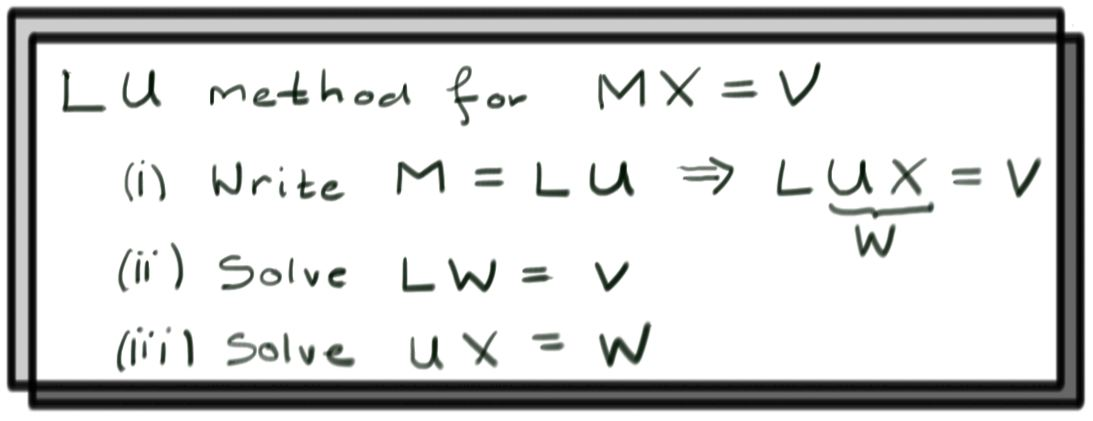
\includegraphics[scale=.3]{\luDecompPath/LU_solution.jpg}
\end{center}
%\end{figure}

\section{Finding an $LU$ Decomposition.}
\label{finding_LU_decomp}
 
For any given matrix, there are actually many different $LU$ decompositions.  However, there is a unique $LU$ decomposition in which the $L$ matrix has ones on the diagonal. In that case $L$ is called a \emph{lower unit triangular matrix}\index{Lower unit triangular matrix}.

To find the $LU$ decomposition, we'll create two sequences of matrices $L_0, L_1, \ldots$ and $U_0, U_1, \ldots$ such that at each step, $L_iU_i=M$.  Each of the $L_i$ will be lower triangular, but only the last $U_i$ will be upper triangular.

Start by setting $L_0=I$ and $U_0=M$, because $L_0U_0=M$. A main concept of this calculation is captured by the following example:

\begin{example}
Consider $$E=\begin{pmatrix}1&0\\\lambda&1\end{pmatrix}\, ,\qquad M=\begin{pmatrix}a&b&c&\cdots\\d&e&f&\cdots\end{pmatrix}\, .$$
Lets compute $EM$
$$
EM=\begin{pmatrix}a&b&c&\cdots\\d+\lambda a&e+\lambda b&f+\lambda c&\cdots\end{pmatrix}\, ,.
$$
Something neat happened here: multiplying $M$ by $E$ performed the row operation $R_2\to R_2+\lambda R-1$ on $M$.
Another interesting fact:
$$
E^{-1}:=\begin{pmatrix}1&0\\-\lambda&1\end{pmatrix}
$$ 
obeys (check this yourself...)
$$
E^{-1} E = 1\, .
$$
Hence $M=E^{-1} E M$ or, writing this out
$$
\begin{pmatrix}a&b&c&\cdots\\d&e&f&\cdots\end{pmatrix}=\begin{pmatrix}1&0\\-\lambda&1\end{pmatrix} \begin{pmatrix}a&b&c&\cdots\\d+\lambda a&e+\lambda b&f+\lambda c&\cdots\end{pmatrix}\, .
$$
Here the matrix on the left is lower triangular, while the matrix on the right has had a row operation performed on it.
\end{example}




\vspace{2mm}
We would like to  use the first row of $U_0$ to zero out the first entry of every row below it.  For our running example, $$U_0=M=\begin{pmatrix}
6 & 18 & 3 \\
2 & 12 & 1 \\
4 & 15 & 3 
\end{pmatrix}\, ,$$ so we would like to perform the row operations $R_2\to R_2 -\frac 13 R_1$ and $R_3\to R_3-\frac 23R_1$.
%so the second row minus $\frac{1}{3}$ of the first row will zero out the first entry in the second row.  Likewise, the third row minus $\frac{2}{3}$ of the first row will zero out the first entry in the third row.
If we perform these row operations on $U_0$ to produce 
$$U_1=\begin{pmatrix}
6 & 18 & 3 \\
0 & 6 & 0 \\
0 & 3 & 1 
\end{pmatrix}\, ,$$
we need to multiply this on the left by a lower triangular matrix $L_1$ so that the product $L_1U_1=M$ still.
The above example shows how to do this:
Set $L_1$ to be the lower triangular matrix whose first column is filled with the minus constants used to zero out the first column of $M$.  Then $$L_1 = \begin{pmatrix}
1 & 0 & 0 \\[1mm]
\frac{1}{3} & 1 & 0 \\[1mm]
\frac{2}{3} & 0 & 1 
\end{pmatrix}\, .$$  
%Set $U_1$ to be the matrix obtained by zeroing out the first column of $M$.  Then $U_1=\begin{pmatrix}
%6 & 18 & 3 \\
%0 & 6 & 0 \\
%0 & 3 & 1 
%\end{pmatrix}$.
By construction $L_1 U_1=M$, but you should compute this yourself as a double check.

Now repeat the process by zeroing the second column of $U_1$ below the diagonal using the second row of $U_1$ using the row operation
$R_3\to R_3-\frac 12 R_2$ to produce
$$U_2=\begin{pmatrix}6&18&3\\0&6&0\\0&0&1\end{pmatrix}\, .$$
The matrix that undoes this row operation is obtained in the same way we found $L_1$ above and is:
$$
\begin{pmatrix}
1&0&0\\
0&1&0\\
0&\frac 12& 0
\end{pmatrix}\, .
$$
Thus our answer for $L_2$ is the product of this matrix with $L_1$, namely
$$
L_2=
\begin{pmatrix}
1 & 0 & 0 \\[1mm]
\frac{1}{3} & 1 & 0 \\[1mm]
\frac{2}{3} & 0 & 1 
\end{pmatrix}\begin{pmatrix}
1&0&0\\
0&1&0\\
0&\frac 12& 0
\end{pmatrix}
=\begin{pmatrix}
1 & 0 & 0 \\[1mm]
\frac{1}{3} & 1 & 0 \\[1mm]
\frac{2}{3} & \frac{1}{2} & 1 
\end{pmatrix}\, .
$$
Notice that it is lower triangular because 

\begin{center}
\textcolor{brown}{THE PRODUCT OF LOWER TRIANGULAR MATRICES IS ALWAYS LOWER TRIANGULAR!}
\end{center}

\noindent
Moreover it is obtained by recording minus the constants used for all our row operations in the appropriate columns (this always works this way).
Moreover, $U_2$ is upper triangular and $M=L_2U_2$, we are done!
Putting this all together we have
$$M=\begin{pmatrix}
6 & 18 & 3 \\
2 & 12 & 1 \\
4 & 15 & 3 
\end{pmatrix}= \begin{pmatrix}
1 & 0 & 0 \\[1mm]
\frac{1}{3} & 1 & 0 \\[1mm]
\frac{2}{3} & \frac{1}{2} & 1 
\end{pmatrix}\begin{pmatrix}
6 & 18 & 3 \\
0 & 6 & 0 \\
0 & 0 & 1 
\end{pmatrix}\, .$$  
%Since $U_2$ is upper-triangular, we're done.  Inserting the new number into $L_1$ to get $L_2$ really is safe: the numbers in the first column don't affect the second column of $U_1$, since the first column of $U_1$ is already zeroed out.

If the matrix you're working with has more than three rows, just continue this process by zeroing out the next column below the diagonal, and repeat until there's nothing left to do.

\videoscriptlink{lu_decomposition_example.mp4}{Another $LU$ decomposition example}{scripts_lu_decomposition_example}

The fractions in the $L$ matrix are admittedly ugly.  For two matrices $LU$, we can multiply one entire column of $L$ by a constant $\lambda$ and divide the corresponding row of $U$ by the same constant without changing the product of the two matrices.  Then:

\begin{eqnarray*}
LU &=& \begin{pmatrix}
1 & 0 & 0 \\[1mm]
\frac{1}{3} & 1 & 0 \\[1mm]
\frac{2}{3} & \frac{1}{2} & 1 
\end{pmatrix}
I
\begin{pmatrix}
6 & 18 & 3 \\
0 & 6 & 0 \\
0 & 0 & 1 
\end{pmatrix} \\
&=&
\begin{pmatrix}
1 & 0 & 0 \\[1mm]
\frac{1}{3} & 1 & 0 \\[1mm]
\frac{2}{3} & \frac{1}{2} & 1 
\end{pmatrix}
\begin{pmatrix}
3 & 0 & 0 \\
0 & 6 & 0 \\
0 & 0 & 1 
\end{pmatrix}
\begin{pmatrix}
\frac{1}{3} & 0 & 0 \\[1mm]
0 & \frac{1}{6} & 0 \\[1mm]
0 & 0 & 1 
\end{pmatrix}
\begin{pmatrix}
6 & 18 & 3 \\
0 & 6 & 0 \\
0 & 0 & 1 
\end{pmatrix} \\
&=&
\begin{pmatrix}
3 & 0 & 0 \\
1 & 6 & 0 \\
2 & 3 & 1 
\end{pmatrix}\begin{pmatrix}
2 & 6 & 1 \\
0 & 1 & 0 \\
0 & 0 & 1 
\end{pmatrix}.
\end{eqnarray*}
The resulting matrix looks nicer, but isn't in standard (lower unit triangular matrix) form.

\reading{11}{2}
%\href{\webworkurl ReadingHomework11/2/}{Reading homework: problem 11.2}

For matrices that are not square, $LU$ decomposition still makes sense.  Given an $m\times n$ matrix $M$, for example we could write $M=LU$ with $L$ a square lower unit triangular matrix, and $U$ a rectangular matrix.  Then $L$ will be an $m\times m$ matrix, and $U$ will be an $m\times n$ matrix (of the same shape as $M$).  From here, the process is exactly the same as for a square matrix.  We create a sequence of matrices $L_i$ and $U_i$ that is eventually the $LU$ decomposition.  Again, we start with $L_0=I$ and $U_0=M$.

\begin{example}
Let's find the $LU$ decomposition of $M=U_0=\begin{pmatrix}
-2 & 1 & 3 \\
-4 & 4 & 1 
\end{pmatrix}$.  Since $M$ is a $2\times 3$ matrix, our decomposition will consist of a $2\times 2$ matrix and a $2\times 3$ matrix.  Then we start with $L_0=I_2=\begin{pmatrix}
1 & 0 \\
0 & 1
\end{pmatrix}$.

The next step is to zero-out the first column of $M$ below the diagonal.  There is only one row to cancel, then, and it can be removed by subtracting $2$ times the first row of $M$ to the second row of $M$.  Then:

\[
L_1=\begin{pmatrix}
1 & 0 \\
2 & 1
\end{pmatrix}, \qquad 
U_1 = \begin{pmatrix}
-2 & 1 & 3 \\
0 & 2 & -5 
\end{pmatrix}
\]
Since $U_1$ is upper triangular, we're done.  With a larger matrix, we would just continue the process.
\end{example}





\section{Block $LDU$ Decomposition}

Let $M$ be a square block matrix with square blocks $X,Y,Z,W$ such that $X^{-1}$ exists.  Then $M$ can be decomposed as a block $LDU$ decomposition, where $D$ is block diagonal, as follows:
\[
M=\begin{pmatrix}
X & Y \\
Z & W
\end{pmatrix}
\]

Then: \[M=\begin{pmatrix}
I &  0 \\
ZX^{-1} & I
\end{pmatrix}\begin{pmatrix}
X & 0 \\
0 & W-ZX^{-1}Y
\end{pmatrix}\begin{pmatrix}
I & X^{-1}Y \\
0 & I
\end{pmatrix}.\]
This can be checked explicitly simply by block-multiplying these three matrices.

\videoscriptlink{lu_decomposition_blocks.mp4}{Block $LDU$ Explanation}{scripts_lu_decomposition_blocks}

\begin{example}
For a $2\times 2$ matrix, we can regard each entry as a block.
\[
\begin{pmatrix}
1 & 2 \\
3 & 4
\end{pmatrix}=
\begin{pmatrix}
1 & 0 \\
3 & 1
\end{pmatrix}
\begin{pmatrix}
1 & 0 \\
0 & -2
\end{pmatrix}
\begin{pmatrix}
1 & 2 \\
0 & 1
\end{pmatrix}
\]
By multiplying the diagonal matrix by the upper triangular matrix, we get the standard $LU$ decomposition of the matrix.
\end{example}


%\section*{References}
%Wikipedia:
%\begin{itemize}
%\item \href{http://en.wikipedia.org/wiki/LU_decomposition}{$LU$ Decomposition}
%\item \href{http://en.wikipedia.org/wiki/Block_LU_decomposition}{Block $LU$ Decomposition}
%\end{itemize}

\section{Review Problems}



\begin{enumerate}

\item Let $D=\begin{pmatrix}
\lambda_1 & \mc0 \\
\mc0 & \lambda_2 \\
\end{pmatrix}$.
\begin{enumerate}
\item Write $D$ in terms of the vectors $e_1$ and $e_2$, and their transposes.
\item Suppose $P=\begin{pmatrix}
a & b \\
c & d \\
\end{pmatrix}$ is invertible.  Show that $D$ is similar to
\[
M=\frac{1}{ad-bc}\begin{pmatrix}
\lambda_1ad-\lambda_2bc & -(\lambda_1-\lambda_2)ab \\[1mm]
(\lambda_1-\lambda_2)cd & -\lambda_1bc + \lambda_2ad
\end{pmatrix}.
\]
\item Suppose the vectors $\rowvec{a,b}$ and $\rowvec{c,d}$ are orthogonal.  What can you say about $M$ in this case? (Hint: think about what \(M^T\) is equal to.)
\end{enumerate}

\phantomnewpage

\item \label{orthogprob} Suppose $S=\{v_1, \ldots, v_n \}$ is an \emph{orthogonal} (not orthonormal) basis for~$\Re^n$.  Then we can write any vector $v$ as $v=\sum_ic^iv_i$ for some constants $c^i$.  Find a formula for the constants $c^i$ in terms of $v$ and the vectors in~$S$.

\Videoscriptlink{orthonormal_bases_hint.mp4}{Hint}{scripts_orthonormal_bases_hint}
\phantomnewpage

\item \label{orthogprojprob} Let $u,v$ be linearly independent vectors in $\Re^3$, and $P=\spa \{ u,v\}$ be the plane spanned by $u$ and $v$.  
\begin{enumerate}
\item Is the vector $v^\bot := v-\frac{u\cdot v}{u\cdot u}u$ in the plane $P$?
\item  What is the (cosine of the) angle between $v^\bot$ and $u$?
\item %Given your solution to the above, 
How can you find a third vector perpendicular to both $u$ and $v^\bot$?
\item  Construct an orthonormal basis for $\Re^3$ from $u$ and $v$.
\item  Test your abstract formul\ae\ starting with 
\[
u=\rowvec{1 , 2 , 0} \text{ and } v=\rowvec{0 , 1 , 1}.
\]
\end{enumerate}

\Videoscriptlink{orthonormal_bases_hint3.mp4}{Hint}{scripts_orthonormal_bases_hint3}

\phantomnewpage



\item Find an orthonormal  basis for $\Re^4$ which includes $(1,1,1,1)$ using the following procedure:\\
\begin{enumerate} 
\item Pick a vector perpendicular to the vector 
$$v_1 =\colvec{1\\1\\1\\1}$$ from the solution set of the matrix equation $$v_1^Tx=0\, .$$ Pick the vector $v_2$ obtained from the standard Gaussian elimination procedure which is the coefficient of $x_2$.
\item Pick a vector perpendicular to both $v_1$ and $v_2$ from the solutions set of the matrix equation $$\colvec{v_1^T\\[1mm]v_2^T}x=0\, .$$ Pick the vector $v_3$ obtained from the standard Gaussian elimination procedure with $x_3$ as the coefficient. 
\item Pick a vector perpendicular to $v_1,v_2,$ and $v_3$ from the solution set of the matrix equation $$\colvec{v_1^T\\[1mm]v_2^T\\[1mm]v_3^T}x=0\, .$$  Pick the vector $v_4$ obtained from the standard Gaussian elimination procedure with $x_3$ as the coefficient. 
\item Normalize the four vectors obtained   above.
\end{enumerate}


\item Use the inner product $$f\cdot g := \int_0^1 f(x)g(x)dx$$  on the vector space $V={\rm span} \{1,x,x^2,x^3\}$ to perform the Gram-Schmidt procedure on the set of vectors $\{1,x,x^2,x^3\}$. 

\item Use the inner product $$f\cdot g := \int_0^{2\pi} f(x)g(x)dx$$  on the vector space $V={\rm span} \{\sin(x),\sin(2x),\sin(3x) \}$ to perform the Gram-Schmidt procedure on the set of vectors $\{\sin(x),\sin(2x),\sin(3x) \}$. \\
Try to build an orthonormal basis for the vector space $$\spa \{ \sin(nx)~| ~n\in \N \}\, .$$
%What do you suspect about the vector space $\spa \{ \sin(nx)~| ~n\in \N \}$?\\
%What do you suspect about the vector space $\spa \{ \sin(ax)~|~ a \in \Re \}$?
\item 
\begin{enumerate}
\item
Show that if $Q$ is an orthogonal $n\times n$ matrix, then $$u\dotprod v = (Qu)\dotprod (Qv)\, ,$$ for any $u,v\in \Re^n$. That is, $Q$ preserves the inner product. 
\item Does $Q$ preserve the outer product? 
\item  If the set of vectors $\{ u_1,\dots,u_n\}$ is orthonormal and $\{ \lambda_1,\cdots,\lambda_n\}$ is a set of numbers, 
then what are the eigenvalues and eigenvectors of the matrix
$M=\sum_{i=1}^n \lambda_i u_i u_i^T$? 
\item How would the eigenvectors and eigenvalues of this matrix change if we replaced  $\{ u_1,\dots,u_n\}$ by $\{ Qu_1,\dots,Q u_n\}$?
\end{enumerate}


\item Carefully write out the Gram-Schmidt procedure for the set of vectors 
$$\left\{ \colvec{1\\1\\1}, \colvec{1\\-1\\1}, \colvec{1\\1\\-1} \right\} \, .$$ Is it possible to rescale the second vector obtained in the procedure to a vector with integer components? 


\item 
\label{basisortho}
\begin{enumerate}
\item Suppose $u$ and $v$ are linearly independent.  Show that $u$ and $v^\perp$ are also linearly independent.  Explain why $\{u, v^\perp\}$ is a basis for $\spa \{u,v\}$.



\Videoscriptlink{gram_schmidt_and_orthogonal_complements_hint.mp4}{Hint}{gram_schmidt_and_orthogonal_complements_hint}

\item Repeat the previous problem, but with three independent vectors $u,v,w$
 where $v^\perp$ and $w^\perp$ are as defined by the Gram-Schmidt procedure. 
\end{enumerate}

\phantomnewpage


\item \label{QRprob} Find the $QR$ factorization of
$$
M=\begin{pmatrix}1&0&\phantom{\!-}2\\-1&2&0\\-1&-2&2
\end{pmatrix}\, .
$$

\phantomnewpage

\item Given any three vectors $u,v,w$, when do $v^\perp$ or $w^\perp$ of the Gram--Schmidt procedure vanish?

\phantomnewpage

\item For $U$ a subspace of $W$, use the subspace theorem to check that $U^\perp$ is a subspace of $W$.

\phantomnewpage


\phantomnewpage

\item %(Extra Credit) 
Let $S_n$ and $A_n$ define the space of $n \times n$ symmetric and anti-symmetric matrices, respectively. These are subspaces of the vector space $M^n_n$ of all $n\times n$ matrices. What is $\dim M^n_n$, $\dim S_n$, and $\dim A_n$? Show that $M^n_n = S_n + A_n$. Define an inner product on square matrices
$$
M\cdot N ={\rm tr} MN\, .
$$
Is $A_n^{\perp}=S_n$? Is $M^n_n = S_n \oplus A_n$?

%\emph{Hint: Note that $\dim S_n = \dim U_n$ where $U_n$ is the vector space of all $n \times n$ upper triangular matrices, and also note that $\dim A_n = \dim \widetilde{U}_n$ where $\widetilde{U}_n$ is the vector space of all strictly $n \times n$ upper triangular matrices (\emph{i.e.} the diagonal entries are all 0).}

\item The vector space $V={\rm span} \{ \sin(t),\sin(2t), \sin(3t) , \sin(3t)\}$ has an inner product: 
$$f\cdot g:=\int _0^{2\pi}f(t)g(t) dt\, .$$ Find the orthogonal compliment to $U={\rm span} \{ \sin(t)+\sin(2t) \}$ in $V$. Express $\sin(t)-\sin(2t)$ as  the sum of vectors from $U$ and $U^\perp$.

\end{enumerate}

\phantomnewpage

\newpage


\chapter{\luDecompTitle}
\label{LUdecomp}

Certain matrices are easier to work with than others.  In this section, we will see how to write any square\footnote{The case where $M$ is not square is dealt with at the end of the lecture.} matrix $M$ as the product of two simpler matrices.  We will write $$M=LU\, ,$$ where:
\begin{itemize}
\item $L$ is \emph{lower triangular}\index{Lower triangular matrix}.  This means that all entries above the main diagonal are zero.  In notation,
$L=(l^i_j)$ with $l^i_j=0$ for all $j>i$.
\[L=\begin{pmatrix}
l^1_1 & 0 & 0 & \cdots \\
l^2_1 & l^2_2 & 0 & \cdots \\
l^3_1 & l^3_2 & l^3_3 & \cdots \\
\vdots & \vdots & \vdots & \ddots \\
\end{pmatrix}
\]

\item $U$ is \emph{upper triangular}\index{Upper triangular matrix}.  This means that all entries below the main diagonal are zero.  In notation,
$U=(u^i_j)$ with $u^i_j=0$ for all $j<i$.
\[U=\begin{pmatrix}
u^1_1 & u^1_2 & u^1_3 & \cdots \\
0 & u^2_2 & u^2_3 & \cdots \\
0 & 0 & u^3_3 & \cdots \\
\vdots & \vdots & \vdots & \ddots \\
\end{pmatrix}
\]
\end{itemize}
$M=LU$ is called an \emph{$LU$ decomposition}\index{LU@$LU$ decomposition} of $M$.

This is a useful trick for  computational reasons; it is much easier to compute the inverse of an upper or lower triangular matrix than general matrices.  Since inverses are useful for solving linear systems, this makes solving any linear system associated to the matrix much faster as well.  The determinant---a very important quantity associated with any square matrix---is very easy to compute for triangular matrices.

\begin{example}
Linear systems associated to upper triangular matrices are very easy to solve by back substitution.
\[
\begin{amatrix}{2}
a & b & 1 \\
0 & c & e \\
\end{amatrix} \ \Rightarrow \ y=\frac{e}{c}\, , \quad x=\frac{1}{a}\left(1-\frac{be}{c}\right)
\]

\[
\begin{amatrix}{3}
1 & 0 & 0 & d \\
a & 1 & 0 & e \\
b & c & 1 & f \\
\end{amatrix} \Rightarrow x=d\, , \qquad y=e-ad\, , \qquad z=f-bd-c(e-ad)
\]
For lower triangular matrices, \emph{back} substitution\index{Back substitution} gives a quick solution; for upper triangular matrices, \emph{forward} substitution\index{Forward substitution} gives the solution.
\end{example}





\section{Using $LU$ Decomposition to Solve Linear Systems}

Suppose we have $M=LU$ and want to solve the system
\[
MX=LUX=V.
\]

\begin{itemize}
\item{Step 1:} Set $W=\colvec{u\\v\\w}=UX$.  

\item{Step 2:} Solve the system $LW=V$.  This should be simple by forward substitution since $L$ is lower triangular.  Suppose the solution to $LW=V$ is $W_0$.  

\item{Step 3:} Now solve the system $UX=W_0$.  This should be easy by backward substitution, since $U$ is upper triangular.  The solution to this system is the solution to the original system.
\end{itemize}
We can think of this as using the matrix $L$ to perform row operations on the matrix $U$ in order to solve the system; this idea also appears in the  study of determinants.

%\href{\webworkurl ReadingHomework11/1/}{Reading homework: problem 11.1}
\reading{11}{1}

\begin{example}
Consider the linear system:
\[
      \begin{linsys}{4}
            6x & +&18y & +&3z         &=& 3  \\[1mm]
            2x & +&12y & +&z	    &=& 19 \\[1mm]
            4x & +&15y & +&3z         &=& 0  
      \end{linsys}
\]

An $LU$ decomposition for the associated matrix $M$ is:
\[
\begin{pmatrix}
6 & 18 & 3 \\
2 & 12 & 1 \\
4 & 15 & 3 
\end{pmatrix} =
\begin{pmatrix}
3 & 0 & 0 \\
1 & 6 & 0 \\
2 & 3 & 1 
\end{pmatrix}
\begin{pmatrix}
2 & 6 & 1 \\
0 & 1 & 0 \\
0 & 0 & 1 
\end{pmatrix}.
\]

\begin{itemize}
\item{Step 1:} \hypertarget{LUproc}{Set} $W=\colvec{u\\v\\w}=UX$.  

\item{Step 2:} Solve the system $LW=V$:

\[
\begin{pmatrix}
3 & 0 & 0 \\
1 & 6 & 0 \\
2 & 3 & 1 
\end{pmatrix}
\colvec{u\\v\\w} =
\colvec{3\\19\\0}
\]

By substitution, we get $u=1$, $v=3$, and $w=-11$.  Then 
\[W_0=\colvec{1\\3\\-11}\]

\item{Step 3:} Solve the system $UX=W_0$.  
\[
\begin{pmatrix}
2 & 6 & 1 \\
0 & 1 & 0 \\
0 & 0 & 1 
\end{pmatrix}
\colvec{x\\y\\z} =
\colvec{1\\3\\-11}
\]
Back substitution gives $z=-11, y=3$, and $x=-3$.  

Then $X=\colvec{-3\\3\\-11}$, and we're done.
\end{itemize}
\end{example}

\videoscriptlink{lu_decomposition_using_lu_decomp.mp4}{Using a $LU$ decomposition}{scripts_lu_decomposition_using_lu_example}

%\begin{figure}
\begin{center}
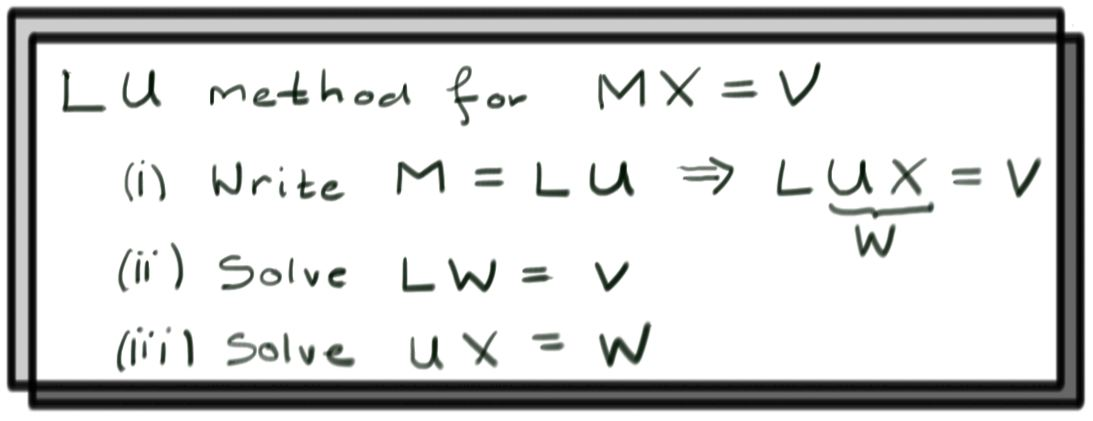
\includegraphics[scale=.3]{\luDecompPath/LU_solution.jpg}
\end{center}
%\end{figure}

\section{Finding an $LU$ Decomposition.}
\label{finding_LU_decomp}
 
For any given matrix, there are actually many different $LU$ decompositions.  However, there is a unique $LU$ decomposition in which the $L$ matrix has ones on the diagonal. In that case $L$ is called a \emph{lower unit triangular matrix}\index{Lower unit triangular matrix}.

To find the $LU$ decomposition, we'll create two sequences of matrices $L_0, L_1, \ldots$ and $U_0, U_1, \ldots$ such that at each step, $L_iU_i=M$.  Each of the $L_i$ will be lower triangular, but only the last $U_i$ will be upper triangular.

Start by setting $L_0=I$ and $U_0=M$, because $L_0U_0=M$. A main concept of this calculation is captured by the following example:

\begin{example}
Consider $$E=\begin{pmatrix}1&0\\\lambda&1\end{pmatrix}\, ,\qquad M=\begin{pmatrix}a&b&c&\cdots\\d&e&f&\cdots\end{pmatrix}\, .$$
Lets compute $EM$
$$
EM=\begin{pmatrix}a&b&c&\cdots\\d+\lambda a&e+\lambda b&f+\lambda c&\cdots\end{pmatrix}\, ,.
$$
Something neat happened here: multiplying $M$ by $E$ performed the row operation $R_2\to R_2+\lambda R-1$ on $M$.
Another interesting fact:
$$
E^{-1}:=\begin{pmatrix}1&0\\-\lambda&1\end{pmatrix}
$$ 
obeys (check this yourself...)
$$
E^{-1} E = 1\, .
$$
Hence $M=E^{-1} E M$ or, writing this out
$$
\begin{pmatrix}a&b&c&\cdots\\d&e&f&\cdots\end{pmatrix}=\begin{pmatrix}1&0\\-\lambda&1\end{pmatrix} \begin{pmatrix}a&b&c&\cdots\\d+\lambda a&e+\lambda b&f+\lambda c&\cdots\end{pmatrix}\, .
$$
Here the matrix on the left is lower triangular, while the matrix on the right has had a row operation performed on it.
\end{example}




\vspace{2mm}
We would like to  use the first row of $U_0$ to zero out the first entry of every row below it.  For our running example, $$U_0=M=\begin{pmatrix}
6 & 18 & 3 \\
2 & 12 & 1 \\
4 & 15 & 3 
\end{pmatrix}\, ,$$ so we would like to perform the row operations $R_2\to R_2 -\frac 13 R_1$ and $R_3\to R_3-\frac 23R_1$.
%so the second row minus $\frac{1}{3}$ of the first row will zero out the first entry in the second row.  Likewise, the third row minus $\frac{2}{3}$ of the first row will zero out the first entry in the third row.
If we perform these row operations on $U_0$ to produce 
$$U_1=\begin{pmatrix}
6 & 18 & 3 \\
0 & 6 & 0 \\
0 & 3 & 1 
\end{pmatrix}\, ,$$
we need to multiply this on the left by a lower triangular matrix $L_1$ so that the product $L_1U_1=M$ still.
The above example shows how to do this:
Set $L_1$ to be the lower triangular matrix whose first column is filled with the minus constants used to zero out the first column of $M$.  Then $$L_1 = \begin{pmatrix}
1 & 0 & 0 \\[1mm]
\frac{1}{3} & 1 & 0 \\[1mm]
\frac{2}{3} & 0 & 1 
\end{pmatrix}\, .$$  
%Set $U_1$ to be the matrix obtained by zeroing out the first column of $M$.  Then $U_1=\begin{pmatrix}
%6 & 18 & 3 \\
%0 & 6 & 0 \\
%0 & 3 & 1 
%\end{pmatrix}$.
By construction $L_1 U_1=M$, but you should compute this yourself as a double check.

Now repeat the process by zeroing the second column of $U_1$ below the diagonal using the second row of $U_1$ using the row operation
$R_3\to R_3-\frac 12 R_2$ to produce
$$U_2=\begin{pmatrix}6&18&3\\0&6&0\\0&0&1\end{pmatrix}\, .$$
The matrix that undoes this row operation is obtained in the same way we found $L_1$ above and is:
$$
\begin{pmatrix}
1&0&0\\
0&1&0\\
0&\frac 12& 0
\end{pmatrix}\, .
$$
Thus our answer for $L_2$ is the product of this matrix with $L_1$, namely
$$
L_2=
\begin{pmatrix}
1 & 0 & 0 \\[1mm]
\frac{1}{3} & 1 & 0 \\[1mm]
\frac{2}{3} & 0 & 1 
\end{pmatrix}\begin{pmatrix}
1&0&0\\
0&1&0\\
0&\frac 12& 0
\end{pmatrix}
=\begin{pmatrix}
1 & 0 & 0 \\[1mm]
\frac{1}{3} & 1 & 0 \\[1mm]
\frac{2}{3} & \frac{1}{2} & 1 
\end{pmatrix}\, .
$$
Notice that it is lower triangular because 

\begin{center}
\textcolor{brown}{THE PRODUCT OF LOWER TRIANGULAR MATRICES IS ALWAYS LOWER TRIANGULAR!}
\end{center}

\noindent
Moreover it is obtained by recording minus the constants used for all our row operations in the appropriate columns (this always works this way).
Moreover, $U_2$ is upper triangular and $M=L_2U_2$, we are done!
Putting this all together we have
$$M=\begin{pmatrix}
6 & 18 & 3 \\
2 & 12 & 1 \\
4 & 15 & 3 
\end{pmatrix}= \begin{pmatrix}
1 & 0 & 0 \\[1mm]
\frac{1}{3} & 1 & 0 \\[1mm]
\frac{2}{3} & \frac{1}{2} & 1 
\end{pmatrix}\begin{pmatrix}
6 & 18 & 3 \\
0 & 6 & 0 \\
0 & 0 & 1 
\end{pmatrix}\, .$$  
%Since $U_2$ is upper-triangular, we're done.  Inserting the new number into $L_1$ to get $L_2$ really is safe: the numbers in the first column don't affect the second column of $U_1$, since the first column of $U_1$ is already zeroed out.

If the matrix you're working with has more than three rows, just continue this process by zeroing out the next column below the diagonal, and repeat until there's nothing left to do.

\videoscriptlink{lu_decomposition_example.mp4}{Another $LU$ decomposition example}{scripts_lu_decomposition_example}

The fractions in the $L$ matrix are admittedly ugly.  For two matrices $LU$, we can multiply one entire column of $L$ by a constant $\lambda$ and divide the corresponding row of $U$ by the same constant without changing the product of the two matrices.  Then:

\begin{eqnarray*}
LU &=& \begin{pmatrix}
1 & 0 & 0 \\[1mm]
\frac{1}{3} & 1 & 0 \\[1mm]
\frac{2}{3} & \frac{1}{2} & 1 
\end{pmatrix}
I
\begin{pmatrix}
6 & 18 & 3 \\
0 & 6 & 0 \\
0 & 0 & 1 
\end{pmatrix} \\
&=&
\begin{pmatrix}
1 & 0 & 0 \\[1mm]
\frac{1}{3} & 1 & 0 \\[1mm]
\frac{2}{3} & \frac{1}{2} & 1 
\end{pmatrix}
\begin{pmatrix}
3 & 0 & 0 \\
0 & 6 & 0 \\
0 & 0 & 1 
\end{pmatrix}
\begin{pmatrix}
\frac{1}{3} & 0 & 0 \\[1mm]
0 & \frac{1}{6} & 0 \\[1mm]
0 & 0 & 1 
\end{pmatrix}
\begin{pmatrix}
6 & 18 & 3 \\
0 & 6 & 0 \\
0 & 0 & 1 
\end{pmatrix} \\
&=&
\begin{pmatrix}
3 & 0 & 0 \\
1 & 6 & 0 \\
2 & 3 & 1 
\end{pmatrix}\begin{pmatrix}
2 & 6 & 1 \\
0 & 1 & 0 \\
0 & 0 & 1 
\end{pmatrix}.
\end{eqnarray*}
The resulting matrix looks nicer, but isn't in standard (lower unit triangular matrix) form.

\reading{11}{2}
%\href{\webworkurl ReadingHomework11/2/}{Reading homework: problem 11.2}

For matrices that are not square, $LU$ decomposition still makes sense.  Given an $m\times n$ matrix $M$, for example we could write $M=LU$ with $L$ a square lower unit triangular matrix, and $U$ a rectangular matrix.  Then $L$ will be an $m\times m$ matrix, and $U$ will be an $m\times n$ matrix (of the same shape as $M$).  From here, the process is exactly the same as for a square matrix.  We create a sequence of matrices $L_i$ and $U_i$ that is eventually the $LU$ decomposition.  Again, we start with $L_0=I$ and $U_0=M$.

\begin{example}
Let's find the $LU$ decomposition of $M=U_0=\begin{pmatrix}
-2 & 1 & 3 \\
-4 & 4 & 1 
\end{pmatrix}$.  Since $M$ is a $2\times 3$ matrix, our decomposition will consist of a $2\times 2$ matrix and a $2\times 3$ matrix.  Then we start with $L_0=I_2=\begin{pmatrix}
1 & 0 \\
0 & 1
\end{pmatrix}$.

The next step is to zero-out the first column of $M$ below the diagonal.  There is only one row to cancel, then, and it can be removed by subtracting $2$ times the first row of $M$ to the second row of $M$.  Then:

\[
L_1=\begin{pmatrix}
1 & 0 \\
2 & 1
\end{pmatrix}, \qquad 
U_1 = \begin{pmatrix}
-2 & 1 & 3 \\
0 & 2 & -5 
\end{pmatrix}
\]
Since $U_1$ is upper triangular, we're done.  With a larger matrix, we would just continue the process.
\end{example}





\section{Block $LDU$ Decomposition}

Let $M$ be a square block matrix with square blocks $X,Y,Z,W$ such that $X^{-1}$ exists.  Then $M$ can be decomposed as a block $LDU$ decomposition, where $D$ is block diagonal, as follows:
\[
M=\begin{pmatrix}
X & Y \\
Z & W
\end{pmatrix}
\]

Then: \[M=\begin{pmatrix}
I &  0 \\
ZX^{-1} & I
\end{pmatrix}\begin{pmatrix}
X & 0 \\
0 & W-ZX^{-1}Y
\end{pmatrix}\begin{pmatrix}
I & X^{-1}Y \\
0 & I
\end{pmatrix}.\]
This can be checked explicitly simply by block-multiplying these three matrices.

\videoscriptlink{lu_decomposition_blocks.mp4}{Block $LDU$ Explanation}{scripts_lu_decomposition_blocks}

\begin{example}
For a $2\times 2$ matrix, we can regard each entry as a block.
\[
\begin{pmatrix}
1 & 2 \\
3 & 4
\end{pmatrix}=
\begin{pmatrix}
1 & 0 \\
3 & 1
\end{pmatrix}
\begin{pmatrix}
1 & 0 \\
0 & -2
\end{pmatrix}
\begin{pmatrix}
1 & 2 \\
0 & 1
\end{pmatrix}
\]
By multiplying the diagonal matrix by the upper triangular matrix, we get the standard $LU$ decomposition of the matrix.
\end{example}


%\section*{References}
%Wikipedia:
%\begin{itemize}
%\item \href{http://en.wikipedia.org/wiki/LU_decomposition}{$LU$ Decomposition}
%\item \href{http://en.wikipedia.org/wiki/Block_LU_decomposition}{Block $LU$ Decomposition}
%\end{itemize}

\section{Review Problems}



\begin{enumerate}

\item Let $D=\begin{pmatrix}
\lambda_1 & \mc0 \\
\mc0 & \lambda_2 \\
\end{pmatrix}$.
\begin{enumerate}
\item Write $D$ in terms of the vectors $e_1$ and $e_2$, and their transposes.
\item Suppose $P=\begin{pmatrix}
a & b \\
c & d \\
\end{pmatrix}$ is invertible.  Show that $D$ is similar to
\[
M=\frac{1}{ad-bc}\begin{pmatrix}
\lambda_1ad-\lambda_2bc & -(\lambda_1-\lambda_2)ab \\[1mm]
(\lambda_1-\lambda_2)cd & -\lambda_1bc + \lambda_2ad
\end{pmatrix}.
\]
\item Suppose the vectors $\rowvec{a,b}$ and $\rowvec{c,d}$ are orthogonal.  What can you say about $M$ in this case? (Hint: think about what \(M^T\) is equal to.)
\end{enumerate}

\phantomnewpage

\item \label{orthogprob} Suppose $S=\{v_1, \ldots, v_n \}$ is an \emph{orthogonal} (not orthonormal) basis for~$\Re^n$.  Then we can write any vector $v$ as $v=\sum_ic^iv_i$ for some constants $c^i$.  Find a formula for the constants $c^i$ in terms of $v$ and the vectors in~$S$.

\Videoscriptlink{orthonormal_bases_hint.mp4}{Hint}{scripts_orthonormal_bases_hint}
\phantomnewpage

\item \label{orthogprojprob} Let $u,v$ be linearly independent vectors in $\Re^3$, and $P=\spa \{ u,v\}$ be the plane spanned by $u$ and $v$.  
\begin{enumerate}
\item Is the vector $v^\bot := v-\frac{u\cdot v}{u\cdot u}u$ in the plane $P$?
\item  What is the (cosine of the) angle between $v^\bot$ and $u$?
\item %Given your solution to the above, 
How can you find a third vector perpendicular to both $u$ and $v^\bot$?
\item  Construct an orthonormal basis for $\Re^3$ from $u$ and $v$.
\item  Test your abstract formul\ae\ starting with 
\[
u=\rowvec{1 , 2 , 0} \text{ and } v=\rowvec{0 , 1 , 1}.
\]
\end{enumerate}

\Videoscriptlink{orthonormal_bases_hint3.mp4}{Hint}{scripts_orthonormal_bases_hint3}

\phantomnewpage



\item Find an orthonormal  basis for $\Re^4$ which includes $(1,1,1,1)$ using the following procedure:\\
\begin{enumerate} 
\item Pick a vector perpendicular to the vector 
$$v_1 =\colvec{1\\1\\1\\1}$$ from the solution set of the matrix equation $$v_1^Tx=0\, .$$ Pick the vector $v_2$ obtained from the standard Gaussian elimination procedure which is the coefficient of $x_2$.
\item Pick a vector perpendicular to both $v_1$ and $v_2$ from the solutions set of the matrix equation $$\colvec{v_1^T\\[1mm]v_2^T}x=0\, .$$ Pick the vector $v_3$ obtained from the standard Gaussian elimination procedure with $x_3$ as the coefficient. 
\item Pick a vector perpendicular to $v_1,v_2,$ and $v_3$ from the solution set of the matrix equation $$\colvec{v_1^T\\[1mm]v_2^T\\[1mm]v_3^T}x=0\, .$$  Pick the vector $v_4$ obtained from the standard Gaussian elimination procedure with $x_3$ as the coefficient. 
\item Normalize the four vectors obtained   above.
\end{enumerate}


\item Use the inner product $$f\cdot g := \int_0^1 f(x)g(x)dx$$  on the vector space $V={\rm span} \{1,x,x^2,x^3\}$ to perform the Gram-Schmidt procedure on the set of vectors $\{1,x,x^2,x^3\}$. 

\item Use the inner product $$f\cdot g := \int_0^{2\pi} f(x)g(x)dx$$  on the vector space $V={\rm span} \{\sin(x),\sin(2x),\sin(3x) \}$ to perform the Gram-Schmidt procedure on the set of vectors $\{\sin(x),\sin(2x),\sin(3x) \}$. \\
Try to build an orthonormal basis for the vector space $$\spa \{ \sin(nx)~| ~n\in \N \}\, .$$
%What do you suspect about the vector space $\spa \{ \sin(nx)~| ~n\in \N \}$?\\
%What do you suspect about the vector space $\spa \{ \sin(ax)~|~ a \in \Re \}$?
\item 
\begin{enumerate}
\item
Show that if $Q$ is an orthogonal $n\times n$ matrix, then $$u\dotprod v = (Qu)\dotprod (Qv)\, ,$$ for any $u,v\in \Re^n$. That is, $Q$ preserves the inner product. 
\item Does $Q$ preserve the outer product? 
\item  If the set of vectors $\{ u_1,\dots,u_n\}$ is orthonormal and $\{ \lambda_1,\cdots,\lambda_n\}$ is a set of numbers, 
then what are the eigenvalues and eigenvectors of the matrix
$M=\sum_{i=1}^n \lambda_i u_i u_i^T$? 
\item How would the eigenvectors and eigenvalues of this matrix change if we replaced  $\{ u_1,\dots,u_n\}$ by $\{ Qu_1,\dots,Q u_n\}$?
\end{enumerate}


\item Carefully write out the Gram-Schmidt procedure for the set of vectors 
$$\left\{ \colvec{1\\1\\1}, \colvec{1\\-1\\1}, \colvec{1\\1\\-1} \right\} \, .$$ Is it possible to rescale the second vector obtained in the procedure to a vector with integer components? 


\item 
\label{basisortho}
\begin{enumerate}
\item Suppose $u$ and $v$ are linearly independent.  Show that $u$ and $v^\perp$ are also linearly independent.  Explain why $\{u, v^\perp\}$ is a basis for $\spa \{u,v\}$.



\Videoscriptlink{gram_schmidt_and_orthogonal_complements_hint.mp4}{Hint}{gram_schmidt_and_orthogonal_complements_hint}

\item Repeat the previous problem, but with three independent vectors $u,v,w$
 where $v^\perp$ and $w^\perp$ are as defined by the Gram-Schmidt procedure. 
\end{enumerate}

\phantomnewpage


\item \label{QRprob} Find the $QR$ factorization of
$$
M=\begin{pmatrix}1&0&\phantom{\!-}2\\-1&2&0\\-1&-2&2
\end{pmatrix}\, .
$$

\phantomnewpage

\item Given any three vectors $u,v,w$, when do $v^\perp$ or $w^\perp$ of the Gram--Schmidt procedure vanish?

\phantomnewpage

\item For $U$ a subspace of $W$, use the subspace theorem to check that $U^\perp$ is a subspace of $W$.

\phantomnewpage


\phantomnewpage

\item %(Extra Credit) 
Let $S_n$ and $A_n$ define the space of $n \times n$ symmetric and anti-symmetric matrices, respectively. These are subspaces of the vector space $M^n_n$ of all $n\times n$ matrices. What is $\dim M^n_n$, $\dim S_n$, and $\dim A_n$? Show that $M^n_n = S_n + A_n$. Define an inner product on square matrices
$$
M\cdot N ={\rm tr} MN\, .
$$
Is $A_n^{\perp}=S_n$? Is $M^n_n = S_n \oplus A_n$?

%\emph{Hint: Note that $\dim S_n = \dim U_n$ where $U_n$ is the vector space of all $n \times n$ upper triangular matrices, and also note that $\dim A_n = \dim \widetilde{U}_n$ where $\widetilde{U}_n$ is the vector space of all strictly $n \times n$ upper triangular matrices (\emph{i.e.} the diagonal entries are all 0).}

\item The vector space $V={\rm span} \{ \sin(t),\sin(2t), \sin(3t) , \sin(3t)\}$ has an inner product: 
$$f\cdot g:=\int _0^{2\pi}f(t)g(t) dt\, .$$ Find the orthogonal compliment to $U={\rm span} \{ \sin(t)+\sin(2t) \}$ in $V$. Express $\sin(t)-\sin(2t)$ as  the sum of vectors from $U$ and $U^\perp$.

\end{enumerate}

\phantomnewpage

\newpage
 %ch8 w2

%\chapter{\luDecompTitle}
\label{LUdecomp}

Certain matrices are easier to work with than others.  In this section, we will see how to write any square\footnote{The case where $M$ is not square is dealt with at the end of the lecture.} matrix $M$ as the product of two simpler matrices.  We will write $$M=LU\, ,$$ where:
\begin{itemize}
\item $L$ is \emph{lower triangular}\index{Lower triangular matrix}.  This means that all entries above the main diagonal are zero.  In notation,
$L=(l^i_j)$ with $l^i_j=0$ for all $j>i$.
\[L=\begin{pmatrix}
l^1_1 & 0 & 0 & \cdots \\
l^2_1 & l^2_2 & 0 & \cdots \\
l^3_1 & l^3_2 & l^3_3 & \cdots \\
\vdots & \vdots & \vdots & \ddots \\
\end{pmatrix}
\]

\item $U$ is \emph{upper triangular}\index{Upper triangular matrix}.  This means that all entries below the main diagonal are zero.  In notation,
$U=(u^i_j)$ with $u^i_j=0$ for all $j<i$.
\[U=\begin{pmatrix}
u^1_1 & u^1_2 & u^1_3 & \cdots \\
0 & u^2_2 & u^2_3 & \cdots \\
0 & 0 & u^3_3 & \cdots \\
\vdots & \vdots & \vdots & \ddots \\
\end{pmatrix}
\]
\end{itemize}
$M=LU$ is called an \emph{$LU$ decomposition}\index{LU@$LU$ decomposition} of $M$.

This is a useful trick for  computational reasons; it is much easier to compute the inverse of an upper or lower triangular matrix than general matrices.  Since inverses are useful for solving linear systems, this makes solving any linear system associated to the matrix much faster as well.  The determinant---a very important quantity associated with any square matrix---is very easy to compute for triangular matrices.

\begin{example}
Linear systems associated to upper triangular matrices are very easy to solve by back substitution.
\[
\begin{amatrix}{2}
a & b & 1 \\
0 & c & e \\
\end{amatrix} \ \Rightarrow \ y=\frac{e}{c}\, , \quad x=\frac{1}{a}\left(1-\frac{be}{c}\right)
\]

\[
\begin{amatrix}{3}
1 & 0 & 0 & d \\
a & 1 & 0 & e \\
b & c & 1 & f \\
\end{amatrix} \Rightarrow x=d\, , \qquad y=e-ad\, , \qquad z=f-bd-c(e-ad)
\]
For lower triangular matrices, \emph{back} substitution\index{Back substitution} gives a quick solution; for upper triangular matrices, \emph{forward} substitution\index{Forward substitution} gives the solution.
\end{example}





\section{Using $LU$ Decomposition to Solve Linear Systems}

Suppose we have $M=LU$ and want to solve the system
\[
MX=LUX=V.
\]

\begin{itemize}
\item{Step 1:} Set $W=\colvec{u\\v\\w}=UX$.  

\item{Step 2:} Solve the system $LW=V$.  This should be simple by forward substitution since $L$ is lower triangular.  Suppose the solution to $LW=V$ is $W_0$.  

\item{Step 3:} Now solve the system $UX=W_0$.  This should be easy by backward substitution, since $U$ is upper triangular.  The solution to this system is the solution to the original system.
\end{itemize}
We can think of this as using the matrix $L$ to perform row operations on the matrix $U$ in order to solve the system; this idea also appears in the  study of determinants.

%\href{\webworkurl ReadingHomework11/1/}{Reading homework: problem 11.1}
\reading{11}{1}

\begin{example}
Consider the linear system:
\[
      \begin{linsys}{4}
            6x & +&18y & +&3z         &=& 3  \\[1mm]
            2x & +&12y & +&z	    &=& 19 \\[1mm]
            4x & +&15y & +&3z         &=& 0  
      \end{linsys}
\]

An $LU$ decomposition for the associated matrix $M$ is:
\[
\begin{pmatrix}
6 & 18 & 3 \\
2 & 12 & 1 \\
4 & 15 & 3 
\end{pmatrix} =
\begin{pmatrix}
3 & 0 & 0 \\
1 & 6 & 0 \\
2 & 3 & 1 
\end{pmatrix}
\begin{pmatrix}
2 & 6 & 1 \\
0 & 1 & 0 \\
0 & 0 & 1 
\end{pmatrix}.
\]

\begin{itemize}
\item{Step 1:} \hypertarget{LUproc}{Set} $W=\colvec{u\\v\\w}=UX$.  

\item{Step 2:} Solve the system $LW=V$:

\[
\begin{pmatrix}
3 & 0 & 0 \\
1 & 6 & 0 \\
2 & 3 & 1 
\end{pmatrix}
\colvec{u\\v\\w} =
\colvec{3\\19\\0}
\]

By substitution, we get $u=1$, $v=3$, and $w=-11$.  Then 
\[W_0=\colvec{1\\3\\-11}\]

\item{Step 3:} Solve the system $UX=W_0$.  
\[
\begin{pmatrix}
2 & 6 & 1 \\
0 & 1 & 0 \\
0 & 0 & 1 
\end{pmatrix}
\colvec{x\\y\\z} =
\colvec{1\\3\\-11}
\]
Back substitution gives $z=-11, y=3$, and $x=-3$.  

Then $X=\colvec{-3\\3\\-11}$, and we're done.
\end{itemize}
\end{example}

\videoscriptlink{lu_decomposition_using_lu_decomp.mp4}{Using a $LU$ decomposition}{scripts_lu_decomposition_using_lu_example}

%\begin{figure}
\begin{center}
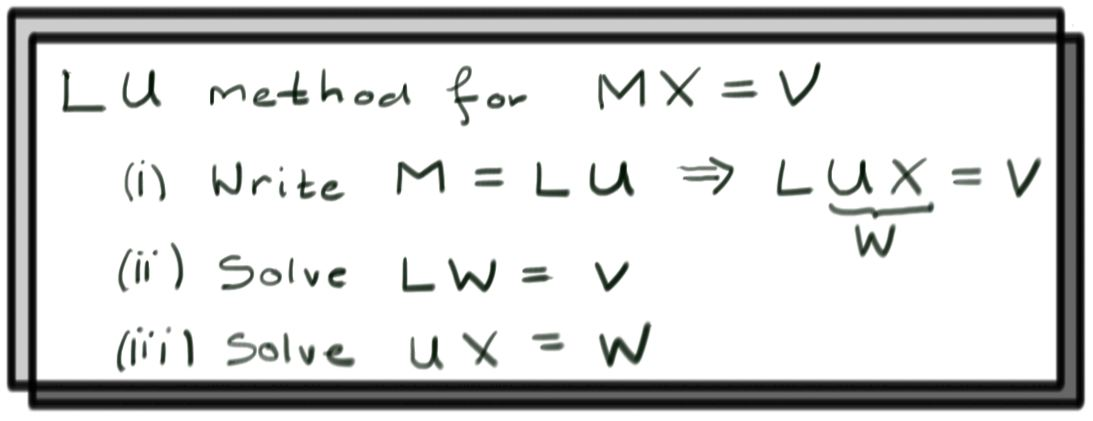
\includegraphics[scale=.3]{\luDecompPath/LU_solution.jpg}
\end{center}
%\end{figure}

\section{Finding an $LU$ Decomposition.}
\label{finding_LU_decomp}
 
For any given matrix, there are actually many different $LU$ decompositions.  However, there is a unique $LU$ decomposition in which the $L$ matrix has ones on the diagonal. In that case $L$ is called a \emph{lower unit triangular matrix}\index{Lower unit triangular matrix}.

To find the $LU$ decomposition, we'll create two sequences of matrices $L_0, L_1, \ldots$ and $U_0, U_1, \ldots$ such that at each step, $L_iU_i=M$.  Each of the $L_i$ will be lower triangular, but only the last $U_i$ will be upper triangular.

Start by setting $L_0=I$ and $U_0=M$, because $L_0U_0=M$. A main concept of this calculation is captured by the following example:

\begin{example}
Consider $$E=\begin{pmatrix}1&0\\\lambda&1\end{pmatrix}\, ,\qquad M=\begin{pmatrix}a&b&c&\cdots\\d&e&f&\cdots\end{pmatrix}\, .$$
Lets compute $EM$
$$
EM=\begin{pmatrix}a&b&c&\cdots\\d+\lambda a&e+\lambda b&f+\lambda c&\cdots\end{pmatrix}\, ,.
$$
Something neat happened here: multiplying $M$ by $E$ performed the row operation $R_2\to R_2+\lambda R-1$ on $M$.
Another interesting fact:
$$
E^{-1}:=\begin{pmatrix}1&0\\-\lambda&1\end{pmatrix}
$$ 
obeys (check this yourself...)
$$
E^{-1} E = 1\, .
$$
Hence $M=E^{-1} E M$ or, writing this out
$$
\begin{pmatrix}a&b&c&\cdots\\d&e&f&\cdots\end{pmatrix}=\begin{pmatrix}1&0\\-\lambda&1\end{pmatrix} \begin{pmatrix}a&b&c&\cdots\\d+\lambda a&e+\lambda b&f+\lambda c&\cdots\end{pmatrix}\, .
$$
Here the matrix on the left is lower triangular, while the matrix on the right has had a row operation performed on it.
\end{example}




\vspace{2mm}
We would like to  use the first row of $U_0$ to zero out the first entry of every row below it.  For our running example, $$U_0=M=\begin{pmatrix}
6 & 18 & 3 \\
2 & 12 & 1 \\
4 & 15 & 3 
\end{pmatrix}\, ,$$ so we would like to perform the row operations $R_2\to R_2 -\frac 13 R_1$ and $R_3\to R_3-\frac 23R_1$.
%so the second row minus $\frac{1}{3}$ of the first row will zero out the first entry in the second row.  Likewise, the third row minus $\frac{2}{3}$ of the first row will zero out the first entry in the third row.
If we perform these row operations on $U_0$ to produce 
$$U_1=\begin{pmatrix}
6 & 18 & 3 \\
0 & 6 & 0 \\
0 & 3 & 1 
\end{pmatrix}\, ,$$
we need to multiply this on the left by a lower triangular matrix $L_1$ so that the product $L_1U_1=M$ still.
The above example shows how to do this:
Set $L_1$ to be the lower triangular matrix whose first column is filled with the minus constants used to zero out the first column of $M$.  Then $$L_1 = \begin{pmatrix}
1 & 0 & 0 \\[1mm]
\frac{1}{3} & 1 & 0 \\[1mm]
\frac{2}{3} & 0 & 1 
\end{pmatrix}\, .$$  
%Set $U_1$ to be the matrix obtained by zeroing out the first column of $M$.  Then $U_1=\begin{pmatrix}
%6 & 18 & 3 \\
%0 & 6 & 0 \\
%0 & 3 & 1 
%\end{pmatrix}$.
By construction $L_1 U_1=M$, but you should compute this yourself as a double check.

Now repeat the process by zeroing the second column of $U_1$ below the diagonal using the second row of $U_1$ using the row operation
$R_3\to R_3-\frac 12 R_2$ to produce
$$U_2=\begin{pmatrix}6&18&3\\0&6&0\\0&0&1\end{pmatrix}\, .$$
The matrix that undoes this row operation is obtained in the same way we found $L_1$ above and is:
$$
\begin{pmatrix}
1&0&0\\
0&1&0\\
0&\frac 12& 0
\end{pmatrix}\, .
$$
Thus our answer for $L_2$ is the product of this matrix with $L_1$, namely
$$
L_2=
\begin{pmatrix}
1 & 0 & 0 \\[1mm]
\frac{1}{3} & 1 & 0 \\[1mm]
\frac{2}{3} & 0 & 1 
\end{pmatrix}\begin{pmatrix}
1&0&0\\
0&1&0\\
0&\frac 12& 0
\end{pmatrix}
=\begin{pmatrix}
1 & 0 & 0 \\[1mm]
\frac{1}{3} & 1 & 0 \\[1mm]
\frac{2}{3} & \frac{1}{2} & 1 
\end{pmatrix}\, .
$$
Notice that it is lower triangular because 

\begin{center}
\textcolor{brown}{THE PRODUCT OF LOWER TRIANGULAR MATRICES IS ALWAYS LOWER TRIANGULAR!}
\end{center}

\noindent
Moreover it is obtained by recording minus the constants used for all our row operations in the appropriate columns (this always works this way).
Moreover, $U_2$ is upper triangular and $M=L_2U_2$, we are done!
Putting this all together we have
$$M=\begin{pmatrix}
6 & 18 & 3 \\
2 & 12 & 1 \\
4 & 15 & 3 
\end{pmatrix}= \begin{pmatrix}
1 & 0 & 0 \\[1mm]
\frac{1}{3} & 1 & 0 \\[1mm]
\frac{2}{3} & \frac{1}{2} & 1 
\end{pmatrix}\begin{pmatrix}
6 & 18 & 3 \\
0 & 6 & 0 \\
0 & 0 & 1 
\end{pmatrix}\, .$$  
%Since $U_2$ is upper-triangular, we're done.  Inserting the new number into $L_1$ to get $L_2$ really is safe: the numbers in the first column don't affect the second column of $U_1$, since the first column of $U_1$ is already zeroed out.

If the matrix you're working with has more than three rows, just continue this process by zeroing out the next column below the diagonal, and repeat until there's nothing left to do.

\videoscriptlink{lu_decomposition_example.mp4}{Another $LU$ decomposition example}{scripts_lu_decomposition_example}

The fractions in the $L$ matrix are admittedly ugly.  For two matrices $LU$, we can multiply one entire column of $L$ by a constant $\lambda$ and divide the corresponding row of $U$ by the same constant without changing the product of the two matrices.  Then:

\begin{eqnarray*}
LU &=& \begin{pmatrix}
1 & 0 & 0 \\[1mm]
\frac{1}{3} & 1 & 0 \\[1mm]
\frac{2}{3} & \frac{1}{2} & 1 
\end{pmatrix}
I
\begin{pmatrix}
6 & 18 & 3 \\
0 & 6 & 0 \\
0 & 0 & 1 
\end{pmatrix} \\
&=&
\begin{pmatrix}
1 & 0 & 0 \\[1mm]
\frac{1}{3} & 1 & 0 \\[1mm]
\frac{2}{3} & \frac{1}{2} & 1 
\end{pmatrix}
\begin{pmatrix}
3 & 0 & 0 \\
0 & 6 & 0 \\
0 & 0 & 1 
\end{pmatrix}
\begin{pmatrix}
\frac{1}{3} & 0 & 0 \\[1mm]
0 & \frac{1}{6} & 0 \\[1mm]
0 & 0 & 1 
\end{pmatrix}
\begin{pmatrix}
6 & 18 & 3 \\
0 & 6 & 0 \\
0 & 0 & 1 
\end{pmatrix} \\
&=&
\begin{pmatrix}
3 & 0 & 0 \\
1 & 6 & 0 \\
2 & 3 & 1 
\end{pmatrix}\begin{pmatrix}
2 & 6 & 1 \\
0 & 1 & 0 \\
0 & 0 & 1 
\end{pmatrix}.
\end{eqnarray*}
The resulting matrix looks nicer, but isn't in standard (lower unit triangular matrix) form.

\reading{11}{2}
%\href{\webworkurl ReadingHomework11/2/}{Reading homework: problem 11.2}

For matrices that are not square, $LU$ decomposition still makes sense.  Given an $m\times n$ matrix $M$, for example we could write $M=LU$ with $L$ a square lower unit triangular matrix, and $U$ a rectangular matrix.  Then $L$ will be an $m\times m$ matrix, and $U$ will be an $m\times n$ matrix (of the same shape as $M$).  From here, the process is exactly the same as for a square matrix.  We create a sequence of matrices $L_i$ and $U_i$ that is eventually the $LU$ decomposition.  Again, we start with $L_0=I$ and $U_0=M$.

\begin{example}
Let's find the $LU$ decomposition of $M=U_0=\begin{pmatrix}
-2 & 1 & 3 \\
-4 & 4 & 1 
\end{pmatrix}$.  Since $M$ is a $2\times 3$ matrix, our decomposition will consist of a $2\times 2$ matrix and a $2\times 3$ matrix.  Then we start with $L_0=I_2=\begin{pmatrix}
1 & 0 \\
0 & 1
\end{pmatrix}$.

The next step is to zero-out the first column of $M$ below the diagonal.  There is only one row to cancel, then, and it can be removed by subtracting $2$ times the first row of $M$ to the second row of $M$.  Then:

\[
L_1=\begin{pmatrix}
1 & 0 \\
2 & 1
\end{pmatrix}, \qquad 
U_1 = \begin{pmatrix}
-2 & 1 & 3 \\
0 & 2 & -5 
\end{pmatrix}
\]
Since $U_1$ is upper triangular, we're done.  With a larger matrix, we would just continue the process.
\end{example}





\section{Block $LDU$ Decomposition}

Let $M$ be a square block matrix with square blocks $X,Y,Z,W$ such that $X^{-1}$ exists.  Then $M$ can be decomposed as a block $LDU$ decomposition, where $D$ is block diagonal, as follows:
\[
M=\begin{pmatrix}
X & Y \\
Z & W
\end{pmatrix}
\]

Then: \[M=\begin{pmatrix}
I &  0 \\
ZX^{-1} & I
\end{pmatrix}\begin{pmatrix}
X & 0 \\
0 & W-ZX^{-1}Y
\end{pmatrix}\begin{pmatrix}
I & X^{-1}Y \\
0 & I
\end{pmatrix}.\]
This can be checked explicitly simply by block-multiplying these three matrices.

\videoscriptlink{lu_decomposition_blocks.mp4}{Block $LDU$ Explanation}{scripts_lu_decomposition_blocks}

\begin{example}
For a $2\times 2$ matrix, we can regard each entry as a block.
\[
\begin{pmatrix}
1 & 2 \\
3 & 4
\end{pmatrix}=
\begin{pmatrix}
1 & 0 \\
3 & 1
\end{pmatrix}
\begin{pmatrix}
1 & 0 \\
0 & -2
\end{pmatrix}
\begin{pmatrix}
1 & 2 \\
0 & 1
\end{pmatrix}
\]
By multiplying the diagonal matrix by the upper triangular matrix, we get the standard $LU$ decomposition of the matrix.
\end{example}


%\section*{References}
%Wikipedia:
%\begin{itemize}
%\item \href{http://en.wikipedia.org/wiki/LU_decomposition}{$LU$ Decomposition}
%\item \href{http://en.wikipedia.org/wiki/Block_LU_decomposition}{Block $LU$ Decomposition}
%\end{itemize}

\section{Review Problems}



\begin{enumerate}

\item Let $D=\begin{pmatrix}
\lambda_1 & \mc0 \\
\mc0 & \lambda_2 \\
\end{pmatrix}$.
\begin{enumerate}
\item Write $D$ in terms of the vectors $e_1$ and $e_2$, and their transposes.
\item Suppose $P=\begin{pmatrix}
a & b \\
c & d \\
\end{pmatrix}$ is invertible.  Show that $D$ is similar to
\[
M=\frac{1}{ad-bc}\begin{pmatrix}
\lambda_1ad-\lambda_2bc & -(\lambda_1-\lambda_2)ab \\[1mm]
(\lambda_1-\lambda_2)cd & -\lambda_1bc + \lambda_2ad
\end{pmatrix}.
\]
\item Suppose the vectors $\rowvec{a,b}$ and $\rowvec{c,d}$ are orthogonal.  What can you say about $M$ in this case? (Hint: think about what \(M^T\) is equal to.)
\end{enumerate}

\phantomnewpage

\item \label{orthogprob} Suppose $S=\{v_1, \ldots, v_n \}$ is an \emph{orthogonal} (not orthonormal) basis for~$\Re^n$.  Then we can write any vector $v$ as $v=\sum_ic^iv_i$ for some constants $c^i$.  Find a formula for the constants $c^i$ in terms of $v$ and the vectors in~$S$.

\Videoscriptlink{orthonormal_bases_hint.mp4}{Hint}{scripts_orthonormal_bases_hint}
\phantomnewpage

\item \label{orthogprojprob} Let $u,v$ be linearly independent vectors in $\Re^3$, and $P=\spa \{ u,v\}$ be the plane spanned by $u$ and $v$.  
\begin{enumerate}
\item Is the vector $v^\bot := v-\frac{u\cdot v}{u\cdot u}u$ in the plane $P$?
\item  What is the (cosine of the) angle between $v^\bot$ and $u$?
\item %Given your solution to the above, 
How can you find a third vector perpendicular to both $u$ and $v^\bot$?
\item  Construct an orthonormal basis for $\Re^3$ from $u$ and $v$.
\item  Test your abstract formul\ae\ starting with 
\[
u=\rowvec{1 , 2 , 0} \text{ and } v=\rowvec{0 , 1 , 1}.
\]
\end{enumerate}

\Videoscriptlink{orthonormal_bases_hint3.mp4}{Hint}{scripts_orthonormal_bases_hint3}

\phantomnewpage



\item Find an orthonormal  basis for $\Re^4$ which includes $(1,1,1,1)$ using the following procedure:\\
\begin{enumerate} 
\item Pick a vector perpendicular to the vector 
$$v_1 =\colvec{1\\1\\1\\1}$$ from the solution set of the matrix equation $$v_1^Tx=0\, .$$ Pick the vector $v_2$ obtained from the standard Gaussian elimination procedure which is the coefficient of $x_2$.
\item Pick a vector perpendicular to both $v_1$ and $v_2$ from the solutions set of the matrix equation $$\colvec{v_1^T\\[1mm]v_2^T}x=0\, .$$ Pick the vector $v_3$ obtained from the standard Gaussian elimination procedure with $x_3$ as the coefficient. 
\item Pick a vector perpendicular to $v_1,v_2,$ and $v_3$ from the solution set of the matrix equation $$\colvec{v_1^T\\[1mm]v_2^T\\[1mm]v_3^T}x=0\, .$$  Pick the vector $v_4$ obtained from the standard Gaussian elimination procedure with $x_3$ as the coefficient. 
\item Normalize the four vectors obtained   above.
\end{enumerate}


\item Use the inner product $$f\cdot g := \int_0^1 f(x)g(x)dx$$  on the vector space $V={\rm span} \{1,x,x^2,x^3\}$ to perform the Gram-Schmidt procedure on the set of vectors $\{1,x,x^2,x^3\}$. 

\item Use the inner product $$f\cdot g := \int_0^{2\pi} f(x)g(x)dx$$  on the vector space $V={\rm span} \{\sin(x),\sin(2x),\sin(3x) \}$ to perform the Gram-Schmidt procedure on the set of vectors $\{\sin(x),\sin(2x),\sin(3x) \}$. \\
Try to build an orthonormal basis for the vector space $$\spa \{ \sin(nx)~| ~n\in \N \}\, .$$
%What do you suspect about the vector space $\spa \{ \sin(nx)~| ~n\in \N \}$?\\
%What do you suspect about the vector space $\spa \{ \sin(ax)~|~ a \in \Re \}$?
\item 
\begin{enumerate}
\item
Show that if $Q$ is an orthogonal $n\times n$ matrix, then $$u\dotprod v = (Qu)\dotprod (Qv)\, ,$$ for any $u,v\in \Re^n$. That is, $Q$ preserves the inner product. 
\item Does $Q$ preserve the outer product? 
\item  If the set of vectors $\{ u_1,\dots,u_n\}$ is orthonormal and $\{ \lambda_1,\cdots,\lambda_n\}$ is a set of numbers, 
then what are the eigenvalues and eigenvectors of the matrix
$M=\sum_{i=1}^n \lambda_i u_i u_i^T$? 
\item How would the eigenvectors and eigenvalues of this matrix change if we replaced  $\{ u_1,\dots,u_n\}$ by $\{ Qu_1,\dots,Q u_n\}$?
\end{enumerate}


\item Carefully write out the Gram-Schmidt procedure for the set of vectors 
$$\left\{ \colvec{1\\1\\1}, \colvec{1\\-1\\1}, \colvec{1\\1\\-1} \right\} \, .$$ Is it possible to rescale the second vector obtained in the procedure to a vector with integer components? 


\item 
\label{basisortho}
\begin{enumerate}
\item Suppose $u$ and $v$ are linearly independent.  Show that $u$ and $v^\perp$ are also linearly independent.  Explain why $\{u, v^\perp\}$ is a basis for $\spa \{u,v\}$.



\Videoscriptlink{gram_schmidt_and_orthogonal_complements_hint.mp4}{Hint}{gram_schmidt_and_orthogonal_complements_hint}

\item Repeat the previous problem, but with three independent vectors $u,v,w$
 where $v^\perp$ and $w^\perp$ are as defined by the Gram-Schmidt procedure. 
\end{enumerate}

\phantomnewpage


\item \label{QRprob} Find the $QR$ factorization of
$$
M=\begin{pmatrix}1&0&\phantom{\!-}2\\-1&2&0\\-1&-2&2
\end{pmatrix}\, .
$$

\phantomnewpage

\item Given any three vectors $u,v,w$, when do $v^\perp$ or $w^\perp$ of the Gram--Schmidt procedure vanish?

\phantomnewpage

\item For $U$ a subspace of $W$, use the subspace theorem to check that $U^\perp$ is a subspace of $W$.

\phantomnewpage


\phantomnewpage

\item %(Extra Credit) 
Let $S_n$ and $A_n$ define the space of $n \times n$ symmetric and anti-symmetric matrices, respectively. These are subspaces of the vector space $M^n_n$ of all $n\times n$ matrices. What is $\dim M^n_n$, $\dim S_n$, and $\dim A_n$? Show that $M^n_n = S_n + A_n$. Define an inner product on square matrices
$$
M\cdot N ={\rm tr} MN\, .
$$
Is $A_n^{\perp}=S_n$? Is $M^n_n = S_n \oplus A_n$?

%\emph{Hint: Note that $\dim S_n = \dim U_n$ where $U_n$ is the vector space of all $n \times n$ upper triangular matrices, and also note that $\dim A_n = \dim \widetilde{U}_n$ where $\widetilde{U}_n$ is the vector space of all strictly $n \times n$ upper triangular matrices (\emph{i.e.} the diagonal entries are all 0).}

\item The vector space $V={\rm span} \{ \sin(t),\sin(2t), \sin(3t) , \sin(3t)\}$ has an inner product: 
$$f\cdot g:=\int _0^{2\pi}f(t)g(t) dt\, .$$ Find the orthogonal compliment to $U={\rm span} \{ \sin(t)+\sin(2t) \}$ in $V$. Express $\sin(t)-\sin(2t)$ as  the sum of vectors from $U$ and $U^\perp$.

\end{enumerate}

\phantomnewpage

\newpage


%\chapter{\luDecompTitle}
\label{LUdecomp}

Certain matrices are easier to work with than others.  In this section, we will see how to write any square\footnote{The case where $M$ is not square is dealt with at the end of the lecture.} matrix $M$ as the product of two simpler matrices.  We will write $$M=LU\, ,$$ where:
\begin{itemize}
\item $L$ is \emph{lower triangular}\index{Lower triangular matrix}.  This means that all entries above the main diagonal are zero.  In notation,
$L=(l^i_j)$ with $l^i_j=0$ for all $j>i$.
\[L=\begin{pmatrix}
l^1_1 & 0 & 0 & \cdots \\
l^2_1 & l^2_2 & 0 & \cdots \\
l^3_1 & l^3_2 & l^3_3 & \cdots \\
\vdots & \vdots & \vdots & \ddots \\
\end{pmatrix}
\]

\item $U$ is \emph{upper triangular}\index{Upper triangular matrix}.  This means that all entries below the main diagonal are zero.  In notation,
$U=(u^i_j)$ with $u^i_j=0$ for all $j<i$.
\[U=\begin{pmatrix}
u^1_1 & u^1_2 & u^1_3 & \cdots \\
0 & u^2_2 & u^2_3 & \cdots \\
0 & 0 & u^3_3 & \cdots \\
\vdots & \vdots & \vdots & \ddots \\
\end{pmatrix}
\]
\end{itemize}
$M=LU$ is called an \emph{$LU$ decomposition}\index{LU@$LU$ decomposition} of $M$.

This is a useful trick for  computational reasons; it is much easier to compute the inverse of an upper or lower triangular matrix than general matrices.  Since inverses are useful for solving linear systems, this makes solving any linear system associated to the matrix much faster as well.  The determinant---a very important quantity associated with any square matrix---is very easy to compute for triangular matrices.

\begin{example}
Linear systems associated to upper triangular matrices are very easy to solve by back substitution.
\[
\begin{amatrix}{2}
a & b & 1 \\
0 & c & e \\
\end{amatrix} \ \Rightarrow \ y=\frac{e}{c}\, , \quad x=\frac{1}{a}\left(1-\frac{be}{c}\right)
\]

\[
\begin{amatrix}{3}
1 & 0 & 0 & d \\
a & 1 & 0 & e \\
b & c & 1 & f \\
\end{amatrix} \Rightarrow x=d\, , \qquad y=e-ad\, , \qquad z=f-bd-c(e-ad)
\]
For lower triangular matrices, \emph{back} substitution\index{Back substitution} gives a quick solution; for upper triangular matrices, \emph{forward} substitution\index{Forward substitution} gives the solution.
\end{example}





\section{Using $LU$ Decomposition to Solve Linear Systems}

Suppose we have $M=LU$ and want to solve the system
\[
MX=LUX=V.
\]

\begin{itemize}
\item{Step 1:} Set $W=\colvec{u\\v\\w}=UX$.  

\item{Step 2:} Solve the system $LW=V$.  This should be simple by forward substitution since $L$ is lower triangular.  Suppose the solution to $LW=V$ is $W_0$.  

\item{Step 3:} Now solve the system $UX=W_0$.  This should be easy by backward substitution, since $U$ is upper triangular.  The solution to this system is the solution to the original system.
\end{itemize}
We can think of this as using the matrix $L$ to perform row operations on the matrix $U$ in order to solve the system; this idea also appears in the  study of determinants.

%\href{\webworkurl ReadingHomework11/1/}{Reading homework: problem 11.1}
\reading{11}{1}

\begin{example}
Consider the linear system:
\[
      \begin{linsys}{4}
            6x & +&18y & +&3z         &=& 3  \\[1mm]
            2x & +&12y & +&z	    &=& 19 \\[1mm]
            4x & +&15y & +&3z         &=& 0  
      \end{linsys}
\]

An $LU$ decomposition for the associated matrix $M$ is:
\[
\begin{pmatrix}
6 & 18 & 3 \\
2 & 12 & 1 \\
4 & 15 & 3 
\end{pmatrix} =
\begin{pmatrix}
3 & 0 & 0 \\
1 & 6 & 0 \\
2 & 3 & 1 
\end{pmatrix}
\begin{pmatrix}
2 & 6 & 1 \\
0 & 1 & 0 \\
0 & 0 & 1 
\end{pmatrix}.
\]

\begin{itemize}
\item{Step 1:} \hypertarget{LUproc}{Set} $W=\colvec{u\\v\\w}=UX$.  

\item{Step 2:} Solve the system $LW=V$:

\[
\begin{pmatrix}
3 & 0 & 0 \\
1 & 6 & 0 \\
2 & 3 & 1 
\end{pmatrix}
\colvec{u\\v\\w} =
\colvec{3\\19\\0}
\]

By substitution, we get $u=1$, $v=3$, and $w=-11$.  Then 
\[W_0=\colvec{1\\3\\-11}\]

\item{Step 3:} Solve the system $UX=W_0$.  
\[
\begin{pmatrix}
2 & 6 & 1 \\
0 & 1 & 0 \\
0 & 0 & 1 
\end{pmatrix}
\colvec{x\\y\\z} =
\colvec{1\\3\\-11}
\]
Back substitution gives $z=-11, y=3$, and $x=-3$.  

Then $X=\colvec{-3\\3\\-11}$, and we're done.
\end{itemize}
\end{example}

\videoscriptlink{lu_decomposition_using_lu_decomp.mp4}{Using a $LU$ decomposition}{scripts_lu_decomposition_using_lu_example}

%\begin{figure}
\begin{center}
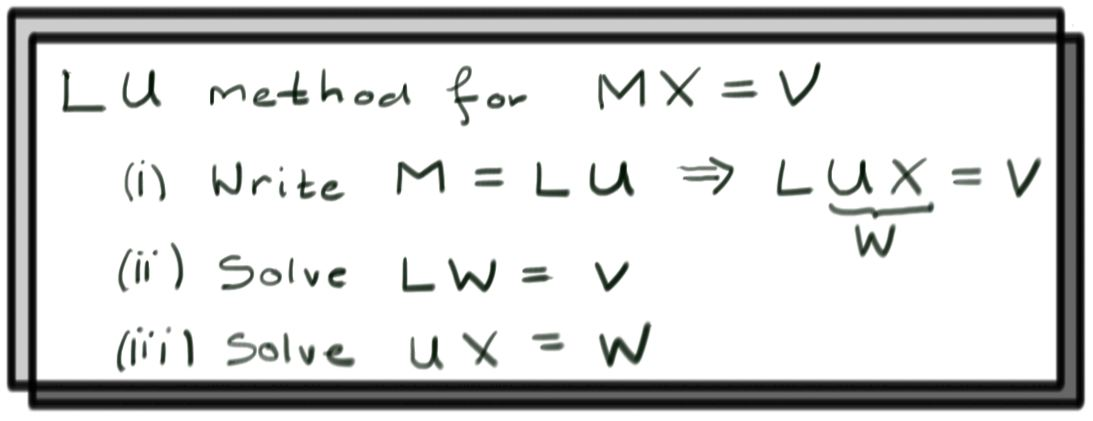
\includegraphics[scale=.3]{\luDecompPath/LU_solution.jpg}
\end{center}
%\end{figure}

\section{Finding an $LU$ Decomposition.}
\label{finding_LU_decomp}
 
For any given matrix, there are actually many different $LU$ decompositions.  However, there is a unique $LU$ decomposition in which the $L$ matrix has ones on the diagonal. In that case $L$ is called a \emph{lower unit triangular matrix}\index{Lower unit triangular matrix}.

To find the $LU$ decomposition, we'll create two sequences of matrices $L_0, L_1, \ldots$ and $U_0, U_1, \ldots$ such that at each step, $L_iU_i=M$.  Each of the $L_i$ will be lower triangular, but only the last $U_i$ will be upper triangular.

Start by setting $L_0=I$ and $U_0=M$, because $L_0U_0=M$. A main concept of this calculation is captured by the following example:

\begin{example}
Consider $$E=\begin{pmatrix}1&0\\\lambda&1\end{pmatrix}\, ,\qquad M=\begin{pmatrix}a&b&c&\cdots\\d&e&f&\cdots\end{pmatrix}\, .$$
Lets compute $EM$
$$
EM=\begin{pmatrix}a&b&c&\cdots\\d+\lambda a&e+\lambda b&f+\lambda c&\cdots\end{pmatrix}\, ,.
$$
Something neat happened here: multiplying $M$ by $E$ performed the row operation $R_2\to R_2+\lambda R-1$ on $M$.
Another interesting fact:
$$
E^{-1}:=\begin{pmatrix}1&0\\-\lambda&1\end{pmatrix}
$$ 
obeys (check this yourself...)
$$
E^{-1} E = 1\, .
$$
Hence $M=E^{-1} E M$ or, writing this out
$$
\begin{pmatrix}a&b&c&\cdots\\d&e&f&\cdots\end{pmatrix}=\begin{pmatrix}1&0\\-\lambda&1\end{pmatrix} \begin{pmatrix}a&b&c&\cdots\\d+\lambda a&e+\lambda b&f+\lambda c&\cdots\end{pmatrix}\, .
$$
Here the matrix on the left is lower triangular, while the matrix on the right has had a row operation performed on it.
\end{example}




\vspace{2mm}
We would like to  use the first row of $U_0$ to zero out the first entry of every row below it.  For our running example, $$U_0=M=\begin{pmatrix}
6 & 18 & 3 \\
2 & 12 & 1 \\
4 & 15 & 3 
\end{pmatrix}\, ,$$ so we would like to perform the row operations $R_2\to R_2 -\frac 13 R_1$ and $R_3\to R_3-\frac 23R_1$.
%so the second row minus $\frac{1}{3}$ of the first row will zero out the first entry in the second row.  Likewise, the third row minus $\frac{2}{3}$ of the first row will zero out the first entry in the third row.
If we perform these row operations on $U_0$ to produce 
$$U_1=\begin{pmatrix}
6 & 18 & 3 \\
0 & 6 & 0 \\
0 & 3 & 1 
\end{pmatrix}\, ,$$
we need to multiply this on the left by a lower triangular matrix $L_1$ so that the product $L_1U_1=M$ still.
The above example shows how to do this:
Set $L_1$ to be the lower triangular matrix whose first column is filled with the minus constants used to zero out the first column of $M$.  Then $$L_1 = \begin{pmatrix}
1 & 0 & 0 \\[1mm]
\frac{1}{3} & 1 & 0 \\[1mm]
\frac{2}{3} & 0 & 1 
\end{pmatrix}\, .$$  
%Set $U_1$ to be the matrix obtained by zeroing out the first column of $M$.  Then $U_1=\begin{pmatrix}
%6 & 18 & 3 \\
%0 & 6 & 0 \\
%0 & 3 & 1 
%\end{pmatrix}$.
By construction $L_1 U_1=M$, but you should compute this yourself as a double check.

Now repeat the process by zeroing the second column of $U_1$ below the diagonal using the second row of $U_1$ using the row operation
$R_3\to R_3-\frac 12 R_2$ to produce
$$U_2=\begin{pmatrix}6&18&3\\0&6&0\\0&0&1\end{pmatrix}\, .$$
The matrix that undoes this row operation is obtained in the same way we found $L_1$ above and is:
$$
\begin{pmatrix}
1&0&0\\
0&1&0\\
0&\frac 12& 0
\end{pmatrix}\, .
$$
Thus our answer for $L_2$ is the product of this matrix with $L_1$, namely
$$
L_2=
\begin{pmatrix}
1 & 0 & 0 \\[1mm]
\frac{1}{3} & 1 & 0 \\[1mm]
\frac{2}{3} & 0 & 1 
\end{pmatrix}\begin{pmatrix}
1&0&0\\
0&1&0\\
0&\frac 12& 0
\end{pmatrix}
=\begin{pmatrix}
1 & 0 & 0 \\[1mm]
\frac{1}{3} & 1 & 0 \\[1mm]
\frac{2}{3} & \frac{1}{2} & 1 
\end{pmatrix}\, .
$$
Notice that it is lower triangular because 

\begin{center}
\textcolor{brown}{THE PRODUCT OF LOWER TRIANGULAR MATRICES IS ALWAYS LOWER TRIANGULAR!}
\end{center}

\noindent
Moreover it is obtained by recording minus the constants used for all our row operations in the appropriate columns (this always works this way).
Moreover, $U_2$ is upper triangular and $M=L_2U_2$, we are done!
Putting this all together we have
$$M=\begin{pmatrix}
6 & 18 & 3 \\
2 & 12 & 1 \\
4 & 15 & 3 
\end{pmatrix}= \begin{pmatrix}
1 & 0 & 0 \\[1mm]
\frac{1}{3} & 1 & 0 \\[1mm]
\frac{2}{3} & \frac{1}{2} & 1 
\end{pmatrix}\begin{pmatrix}
6 & 18 & 3 \\
0 & 6 & 0 \\
0 & 0 & 1 
\end{pmatrix}\, .$$  
%Since $U_2$ is upper-triangular, we're done.  Inserting the new number into $L_1$ to get $L_2$ really is safe: the numbers in the first column don't affect the second column of $U_1$, since the first column of $U_1$ is already zeroed out.

If the matrix you're working with has more than three rows, just continue this process by zeroing out the next column below the diagonal, and repeat until there's nothing left to do.

\videoscriptlink{lu_decomposition_example.mp4}{Another $LU$ decomposition example}{scripts_lu_decomposition_example}

The fractions in the $L$ matrix are admittedly ugly.  For two matrices $LU$, we can multiply one entire column of $L$ by a constant $\lambda$ and divide the corresponding row of $U$ by the same constant without changing the product of the two matrices.  Then:

\begin{eqnarray*}
LU &=& \begin{pmatrix}
1 & 0 & 0 \\[1mm]
\frac{1}{3} & 1 & 0 \\[1mm]
\frac{2}{3} & \frac{1}{2} & 1 
\end{pmatrix}
I
\begin{pmatrix}
6 & 18 & 3 \\
0 & 6 & 0 \\
0 & 0 & 1 
\end{pmatrix} \\
&=&
\begin{pmatrix}
1 & 0 & 0 \\[1mm]
\frac{1}{3} & 1 & 0 \\[1mm]
\frac{2}{3} & \frac{1}{2} & 1 
\end{pmatrix}
\begin{pmatrix}
3 & 0 & 0 \\
0 & 6 & 0 \\
0 & 0 & 1 
\end{pmatrix}
\begin{pmatrix}
\frac{1}{3} & 0 & 0 \\[1mm]
0 & \frac{1}{6} & 0 \\[1mm]
0 & 0 & 1 
\end{pmatrix}
\begin{pmatrix}
6 & 18 & 3 \\
0 & 6 & 0 \\
0 & 0 & 1 
\end{pmatrix} \\
&=&
\begin{pmatrix}
3 & 0 & 0 \\
1 & 6 & 0 \\
2 & 3 & 1 
\end{pmatrix}\begin{pmatrix}
2 & 6 & 1 \\
0 & 1 & 0 \\
0 & 0 & 1 
\end{pmatrix}.
\end{eqnarray*}
The resulting matrix looks nicer, but isn't in standard (lower unit triangular matrix) form.

\reading{11}{2}
%\href{\webworkurl ReadingHomework11/2/}{Reading homework: problem 11.2}

For matrices that are not square, $LU$ decomposition still makes sense.  Given an $m\times n$ matrix $M$, for example we could write $M=LU$ with $L$ a square lower unit triangular matrix, and $U$ a rectangular matrix.  Then $L$ will be an $m\times m$ matrix, and $U$ will be an $m\times n$ matrix (of the same shape as $M$).  From here, the process is exactly the same as for a square matrix.  We create a sequence of matrices $L_i$ and $U_i$ that is eventually the $LU$ decomposition.  Again, we start with $L_0=I$ and $U_0=M$.

\begin{example}
Let's find the $LU$ decomposition of $M=U_0=\begin{pmatrix}
-2 & 1 & 3 \\
-4 & 4 & 1 
\end{pmatrix}$.  Since $M$ is a $2\times 3$ matrix, our decomposition will consist of a $2\times 2$ matrix and a $2\times 3$ matrix.  Then we start with $L_0=I_2=\begin{pmatrix}
1 & 0 \\
0 & 1
\end{pmatrix}$.

The next step is to zero-out the first column of $M$ below the diagonal.  There is only one row to cancel, then, and it can be removed by subtracting $2$ times the first row of $M$ to the second row of $M$.  Then:

\[
L_1=\begin{pmatrix}
1 & 0 \\
2 & 1
\end{pmatrix}, \qquad 
U_1 = \begin{pmatrix}
-2 & 1 & 3 \\
0 & 2 & -5 
\end{pmatrix}
\]
Since $U_1$ is upper triangular, we're done.  With a larger matrix, we would just continue the process.
\end{example}





\section{Block $LDU$ Decomposition}

Let $M$ be a square block matrix with square blocks $X,Y,Z,W$ such that $X^{-1}$ exists.  Then $M$ can be decomposed as a block $LDU$ decomposition, where $D$ is block diagonal, as follows:
\[
M=\begin{pmatrix}
X & Y \\
Z & W
\end{pmatrix}
\]

Then: \[M=\begin{pmatrix}
I &  0 \\
ZX^{-1} & I
\end{pmatrix}\begin{pmatrix}
X & 0 \\
0 & W-ZX^{-1}Y
\end{pmatrix}\begin{pmatrix}
I & X^{-1}Y \\
0 & I
\end{pmatrix}.\]
This can be checked explicitly simply by block-multiplying these three matrices.

\videoscriptlink{lu_decomposition_blocks.mp4}{Block $LDU$ Explanation}{scripts_lu_decomposition_blocks}

\begin{example}
For a $2\times 2$ matrix, we can regard each entry as a block.
\[
\begin{pmatrix}
1 & 2 \\
3 & 4
\end{pmatrix}=
\begin{pmatrix}
1 & 0 \\
3 & 1
\end{pmatrix}
\begin{pmatrix}
1 & 0 \\
0 & -2
\end{pmatrix}
\begin{pmatrix}
1 & 2 \\
0 & 1
\end{pmatrix}
\]
By multiplying the diagonal matrix by the upper triangular matrix, we get the standard $LU$ decomposition of the matrix.
\end{example}


%\section*{References}
%Wikipedia:
%\begin{itemize}
%\item \href{http://en.wikipedia.org/wiki/LU_decomposition}{$LU$ Decomposition}
%\item \href{http://en.wikipedia.org/wiki/Block_LU_decomposition}{Block $LU$ Decomposition}
%\end{itemize}

\section{Review Problems}



\begin{enumerate}

\item Let $D=\begin{pmatrix}
\lambda_1 & \mc0 \\
\mc0 & \lambda_2 \\
\end{pmatrix}$.
\begin{enumerate}
\item Write $D$ in terms of the vectors $e_1$ and $e_2$, and their transposes.
\item Suppose $P=\begin{pmatrix}
a & b \\
c & d \\
\end{pmatrix}$ is invertible.  Show that $D$ is similar to
\[
M=\frac{1}{ad-bc}\begin{pmatrix}
\lambda_1ad-\lambda_2bc & -(\lambda_1-\lambda_2)ab \\[1mm]
(\lambda_1-\lambda_2)cd & -\lambda_1bc + \lambda_2ad
\end{pmatrix}.
\]
\item Suppose the vectors $\rowvec{a,b}$ and $\rowvec{c,d}$ are orthogonal.  What can you say about $M$ in this case? (Hint: think about what \(M^T\) is equal to.)
\end{enumerate}

\phantomnewpage

\item \label{orthogprob} Suppose $S=\{v_1, \ldots, v_n \}$ is an \emph{orthogonal} (not orthonormal) basis for~$\Re^n$.  Then we can write any vector $v$ as $v=\sum_ic^iv_i$ for some constants $c^i$.  Find a formula for the constants $c^i$ in terms of $v$ and the vectors in~$S$.

\Videoscriptlink{orthonormal_bases_hint.mp4}{Hint}{scripts_orthonormal_bases_hint}
\phantomnewpage

\item \label{orthogprojprob} Let $u,v$ be linearly independent vectors in $\Re^3$, and $P=\spa \{ u,v\}$ be the plane spanned by $u$ and $v$.  
\begin{enumerate}
\item Is the vector $v^\bot := v-\frac{u\cdot v}{u\cdot u}u$ in the plane $P$?
\item  What is the (cosine of the) angle between $v^\bot$ and $u$?
\item %Given your solution to the above, 
How can you find a third vector perpendicular to both $u$ and $v^\bot$?
\item  Construct an orthonormal basis for $\Re^3$ from $u$ and $v$.
\item  Test your abstract formul\ae\ starting with 
\[
u=\rowvec{1 , 2 , 0} \text{ and } v=\rowvec{0 , 1 , 1}.
\]
\end{enumerate}

\Videoscriptlink{orthonormal_bases_hint3.mp4}{Hint}{scripts_orthonormal_bases_hint3}

\phantomnewpage



\item Find an orthonormal  basis for $\Re^4$ which includes $(1,1,1,1)$ using the following procedure:\\
\begin{enumerate} 
\item Pick a vector perpendicular to the vector 
$$v_1 =\colvec{1\\1\\1\\1}$$ from the solution set of the matrix equation $$v_1^Tx=0\, .$$ Pick the vector $v_2$ obtained from the standard Gaussian elimination procedure which is the coefficient of $x_2$.
\item Pick a vector perpendicular to both $v_1$ and $v_2$ from the solutions set of the matrix equation $$\colvec{v_1^T\\[1mm]v_2^T}x=0\, .$$ Pick the vector $v_3$ obtained from the standard Gaussian elimination procedure with $x_3$ as the coefficient. 
\item Pick a vector perpendicular to $v_1,v_2,$ and $v_3$ from the solution set of the matrix equation $$\colvec{v_1^T\\[1mm]v_2^T\\[1mm]v_3^T}x=0\, .$$  Pick the vector $v_4$ obtained from the standard Gaussian elimination procedure with $x_3$ as the coefficient. 
\item Normalize the four vectors obtained   above.
\end{enumerate}


\item Use the inner product $$f\cdot g := \int_0^1 f(x)g(x)dx$$  on the vector space $V={\rm span} \{1,x,x^2,x^3\}$ to perform the Gram-Schmidt procedure on the set of vectors $\{1,x,x^2,x^3\}$. 

\item Use the inner product $$f\cdot g := \int_0^{2\pi} f(x)g(x)dx$$  on the vector space $V={\rm span} \{\sin(x),\sin(2x),\sin(3x) \}$ to perform the Gram-Schmidt procedure on the set of vectors $\{\sin(x),\sin(2x),\sin(3x) \}$. \\
Try to build an orthonormal basis for the vector space $$\spa \{ \sin(nx)~| ~n\in \N \}\, .$$
%What do you suspect about the vector space $\spa \{ \sin(nx)~| ~n\in \N \}$?\\
%What do you suspect about the vector space $\spa \{ \sin(ax)~|~ a \in \Re \}$?
\item 
\begin{enumerate}
\item
Show that if $Q$ is an orthogonal $n\times n$ matrix, then $$u\dotprod v = (Qu)\dotprod (Qv)\, ,$$ for any $u,v\in \Re^n$. That is, $Q$ preserves the inner product. 
\item Does $Q$ preserve the outer product? 
\item  If the set of vectors $\{ u_1,\dots,u_n\}$ is orthonormal and $\{ \lambda_1,\cdots,\lambda_n\}$ is a set of numbers, 
then what are the eigenvalues and eigenvectors of the matrix
$M=\sum_{i=1}^n \lambda_i u_i u_i^T$? 
\item How would the eigenvectors and eigenvalues of this matrix change if we replaced  $\{ u_1,\dots,u_n\}$ by $\{ Qu_1,\dots,Q u_n\}$?
\end{enumerate}


\item Carefully write out the Gram-Schmidt procedure for the set of vectors 
$$\left\{ \colvec{1\\1\\1}, \colvec{1\\-1\\1}, \colvec{1\\1\\-1} \right\} \, .$$ Is it possible to rescale the second vector obtained in the procedure to a vector with integer components? 


\item 
\label{basisortho}
\begin{enumerate}
\item Suppose $u$ and $v$ are linearly independent.  Show that $u$ and $v^\perp$ are also linearly independent.  Explain why $\{u, v^\perp\}$ is a basis for $\spa \{u,v\}$.



\Videoscriptlink{gram_schmidt_and_orthogonal_complements_hint.mp4}{Hint}{gram_schmidt_and_orthogonal_complements_hint}

\item Repeat the previous problem, but with three independent vectors $u,v,w$
 where $v^\perp$ and $w^\perp$ are as defined by the Gram-Schmidt procedure. 
\end{enumerate}

\phantomnewpage


\item \label{QRprob} Find the $QR$ factorization of
$$
M=\begin{pmatrix}1&0&\phantom{\!-}2\\-1&2&0\\-1&-2&2
\end{pmatrix}\, .
$$

\phantomnewpage

\item Given any three vectors $u,v,w$, when do $v^\perp$ or $w^\perp$ of the Gram--Schmidt procedure vanish?

\phantomnewpage

\item For $U$ a subspace of $W$, use the subspace theorem to check that $U^\perp$ is a subspace of $W$.

\phantomnewpage


\phantomnewpage

\item %(Extra Credit) 
Let $S_n$ and $A_n$ define the space of $n \times n$ symmetric and anti-symmetric matrices, respectively. These are subspaces of the vector space $M^n_n$ of all $n\times n$ matrices. What is $\dim M^n_n$, $\dim S_n$, and $\dim A_n$? Show that $M^n_n = S_n + A_n$. Define an inner product on square matrices
$$
M\cdot N ={\rm tr} MN\, .
$$
Is $A_n^{\perp}=S_n$? Is $M^n_n = S_n \oplus A_n$?

%\emph{Hint: Note that $\dim S_n = \dim U_n$ where $U_n$ is the vector space of all $n \times n$ upper triangular matrices, and also note that $\dim A_n = \dim \widetilde{U}_n$ where $\widetilde{U}_n$ is the vector space of all strictly $n \times n$ upper triangular matrices (\emph{i.e.} the diagonal entries are all 0).}

\item The vector space $V={\rm span} \{ \sin(t),\sin(2t), \sin(3t) , \sin(3t)\}$ has an inner product: 
$$f\cdot g:=\int _0^{2\pi}f(t)g(t) dt\, .$$ Find the orthogonal compliment to $U={\rm span} \{ \sin(t)+\sin(2t) \}$ in $V$. Express $\sin(t)-\sin(2t)$ as  the sum of vectors from $U$ and $U^\perp$.

\end{enumerate}

\phantomnewpage

\newpage


%\chapter{\luDecompTitle}
\label{LUdecomp}

Certain matrices are easier to work with than others.  In this section, we will see how to write any square\footnote{The case where $M$ is not square is dealt with at the end of the lecture.} matrix $M$ as the product of two simpler matrices.  We will write $$M=LU\, ,$$ where:
\begin{itemize}
\item $L$ is \emph{lower triangular}\index{Lower triangular matrix}.  This means that all entries above the main diagonal are zero.  In notation,
$L=(l^i_j)$ with $l^i_j=0$ for all $j>i$.
\[L=\begin{pmatrix}
l^1_1 & 0 & 0 & \cdots \\
l^2_1 & l^2_2 & 0 & \cdots \\
l^3_1 & l^3_2 & l^3_3 & \cdots \\
\vdots & \vdots & \vdots & \ddots \\
\end{pmatrix}
\]

\item $U$ is \emph{upper triangular}\index{Upper triangular matrix}.  This means that all entries below the main diagonal are zero.  In notation,
$U=(u^i_j)$ with $u^i_j=0$ for all $j<i$.
\[U=\begin{pmatrix}
u^1_1 & u^1_2 & u^1_3 & \cdots \\
0 & u^2_2 & u^2_3 & \cdots \\
0 & 0 & u^3_3 & \cdots \\
\vdots & \vdots & \vdots & \ddots \\
\end{pmatrix}
\]
\end{itemize}
$M=LU$ is called an \emph{$LU$ decomposition}\index{LU@$LU$ decomposition} of $M$.

This is a useful trick for  computational reasons; it is much easier to compute the inverse of an upper or lower triangular matrix than general matrices.  Since inverses are useful for solving linear systems, this makes solving any linear system associated to the matrix much faster as well.  The determinant---a very important quantity associated with any square matrix---is very easy to compute for triangular matrices.

\begin{example}
Linear systems associated to upper triangular matrices are very easy to solve by back substitution.
\[
\begin{amatrix}{2}
a & b & 1 \\
0 & c & e \\
\end{amatrix} \ \Rightarrow \ y=\frac{e}{c}\, , \quad x=\frac{1}{a}\left(1-\frac{be}{c}\right)
\]

\[
\begin{amatrix}{3}
1 & 0 & 0 & d \\
a & 1 & 0 & e \\
b & c & 1 & f \\
\end{amatrix} \Rightarrow x=d\, , \qquad y=e-ad\, , \qquad z=f-bd-c(e-ad)
\]
For lower triangular matrices, \emph{back} substitution\index{Back substitution} gives a quick solution; for upper triangular matrices, \emph{forward} substitution\index{Forward substitution} gives the solution.
\end{example}





\section{Using $LU$ Decomposition to Solve Linear Systems}

Suppose we have $M=LU$ and want to solve the system
\[
MX=LUX=V.
\]

\begin{itemize}
\item{Step 1:} Set $W=\colvec{u\\v\\w}=UX$.  

\item{Step 2:} Solve the system $LW=V$.  This should be simple by forward substitution since $L$ is lower triangular.  Suppose the solution to $LW=V$ is $W_0$.  

\item{Step 3:} Now solve the system $UX=W_0$.  This should be easy by backward substitution, since $U$ is upper triangular.  The solution to this system is the solution to the original system.
\end{itemize}
We can think of this as using the matrix $L$ to perform row operations on the matrix $U$ in order to solve the system; this idea also appears in the  study of determinants.

%\href{\webworkurl ReadingHomework11/1/}{Reading homework: problem 11.1}
\reading{11}{1}

\begin{example}
Consider the linear system:
\[
      \begin{linsys}{4}
            6x & +&18y & +&3z         &=& 3  \\[1mm]
            2x & +&12y & +&z	    &=& 19 \\[1mm]
            4x & +&15y & +&3z         &=& 0  
      \end{linsys}
\]

An $LU$ decomposition for the associated matrix $M$ is:
\[
\begin{pmatrix}
6 & 18 & 3 \\
2 & 12 & 1 \\
4 & 15 & 3 
\end{pmatrix} =
\begin{pmatrix}
3 & 0 & 0 \\
1 & 6 & 0 \\
2 & 3 & 1 
\end{pmatrix}
\begin{pmatrix}
2 & 6 & 1 \\
0 & 1 & 0 \\
0 & 0 & 1 
\end{pmatrix}.
\]

\begin{itemize}
\item{Step 1:} \hypertarget{LUproc}{Set} $W=\colvec{u\\v\\w}=UX$.  

\item{Step 2:} Solve the system $LW=V$:

\[
\begin{pmatrix}
3 & 0 & 0 \\
1 & 6 & 0 \\
2 & 3 & 1 
\end{pmatrix}
\colvec{u\\v\\w} =
\colvec{3\\19\\0}
\]

By substitution, we get $u=1$, $v=3$, and $w=-11$.  Then 
\[W_0=\colvec{1\\3\\-11}\]

\item{Step 3:} Solve the system $UX=W_0$.  
\[
\begin{pmatrix}
2 & 6 & 1 \\
0 & 1 & 0 \\
0 & 0 & 1 
\end{pmatrix}
\colvec{x\\y\\z} =
\colvec{1\\3\\-11}
\]
Back substitution gives $z=-11, y=3$, and $x=-3$.  

Then $X=\colvec{-3\\3\\-11}$, and we're done.
\end{itemize}
\end{example}

\videoscriptlink{lu_decomposition_using_lu_decomp.mp4}{Using a $LU$ decomposition}{scripts_lu_decomposition_using_lu_example}

%\begin{figure}
\begin{center}
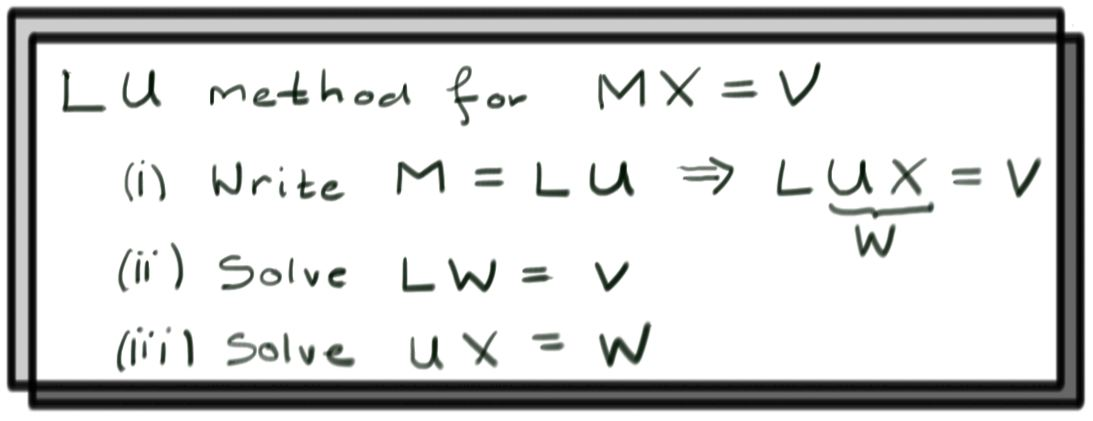
\includegraphics[scale=.3]{\luDecompPath/LU_solution.jpg}
\end{center}
%\end{figure}

\section{Finding an $LU$ Decomposition.}
\label{finding_LU_decomp}
 
For any given matrix, there are actually many different $LU$ decompositions.  However, there is a unique $LU$ decomposition in which the $L$ matrix has ones on the diagonal. In that case $L$ is called a \emph{lower unit triangular matrix}\index{Lower unit triangular matrix}.

To find the $LU$ decomposition, we'll create two sequences of matrices $L_0, L_1, \ldots$ and $U_0, U_1, \ldots$ such that at each step, $L_iU_i=M$.  Each of the $L_i$ will be lower triangular, but only the last $U_i$ will be upper triangular.

Start by setting $L_0=I$ and $U_0=M$, because $L_0U_0=M$. A main concept of this calculation is captured by the following example:

\begin{example}
Consider $$E=\begin{pmatrix}1&0\\\lambda&1\end{pmatrix}\, ,\qquad M=\begin{pmatrix}a&b&c&\cdots\\d&e&f&\cdots\end{pmatrix}\, .$$
Lets compute $EM$
$$
EM=\begin{pmatrix}a&b&c&\cdots\\d+\lambda a&e+\lambda b&f+\lambda c&\cdots\end{pmatrix}\, ,.
$$
Something neat happened here: multiplying $M$ by $E$ performed the row operation $R_2\to R_2+\lambda R-1$ on $M$.
Another interesting fact:
$$
E^{-1}:=\begin{pmatrix}1&0\\-\lambda&1\end{pmatrix}
$$ 
obeys (check this yourself...)
$$
E^{-1} E = 1\, .
$$
Hence $M=E^{-1} E M$ or, writing this out
$$
\begin{pmatrix}a&b&c&\cdots\\d&e&f&\cdots\end{pmatrix}=\begin{pmatrix}1&0\\-\lambda&1\end{pmatrix} \begin{pmatrix}a&b&c&\cdots\\d+\lambda a&e+\lambda b&f+\lambda c&\cdots\end{pmatrix}\, .
$$
Here the matrix on the left is lower triangular, while the matrix on the right has had a row operation performed on it.
\end{example}




\vspace{2mm}
We would like to  use the first row of $U_0$ to zero out the first entry of every row below it.  For our running example, $$U_0=M=\begin{pmatrix}
6 & 18 & 3 \\
2 & 12 & 1 \\
4 & 15 & 3 
\end{pmatrix}\, ,$$ so we would like to perform the row operations $R_2\to R_2 -\frac 13 R_1$ and $R_3\to R_3-\frac 23R_1$.
%so the second row minus $\frac{1}{3}$ of the first row will zero out the first entry in the second row.  Likewise, the third row minus $\frac{2}{3}$ of the first row will zero out the first entry in the third row.
If we perform these row operations on $U_0$ to produce 
$$U_1=\begin{pmatrix}
6 & 18 & 3 \\
0 & 6 & 0 \\
0 & 3 & 1 
\end{pmatrix}\, ,$$
we need to multiply this on the left by a lower triangular matrix $L_1$ so that the product $L_1U_1=M$ still.
The above example shows how to do this:
Set $L_1$ to be the lower triangular matrix whose first column is filled with the minus constants used to zero out the first column of $M$.  Then $$L_1 = \begin{pmatrix}
1 & 0 & 0 \\[1mm]
\frac{1}{3} & 1 & 0 \\[1mm]
\frac{2}{3} & 0 & 1 
\end{pmatrix}\, .$$  
%Set $U_1$ to be the matrix obtained by zeroing out the first column of $M$.  Then $U_1=\begin{pmatrix}
%6 & 18 & 3 \\
%0 & 6 & 0 \\
%0 & 3 & 1 
%\end{pmatrix}$.
By construction $L_1 U_1=M$, but you should compute this yourself as a double check.

Now repeat the process by zeroing the second column of $U_1$ below the diagonal using the second row of $U_1$ using the row operation
$R_3\to R_3-\frac 12 R_2$ to produce
$$U_2=\begin{pmatrix}6&18&3\\0&6&0\\0&0&1\end{pmatrix}\, .$$
The matrix that undoes this row operation is obtained in the same way we found $L_1$ above and is:
$$
\begin{pmatrix}
1&0&0\\
0&1&0\\
0&\frac 12& 0
\end{pmatrix}\, .
$$
Thus our answer for $L_2$ is the product of this matrix with $L_1$, namely
$$
L_2=
\begin{pmatrix}
1 & 0 & 0 \\[1mm]
\frac{1}{3} & 1 & 0 \\[1mm]
\frac{2}{3} & 0 & 1 
\end{pmatrix}\begin{pmatrix}
1&0&0\\
0&1&0\\
0&\frac 12& 0
\end{pmatrix}
=\begin{pmatrix}
1 & 0 & 0 \\[1mm]
\frac{1}{3} & 1 & 0 \\[1mm]
\frac{2}{3} & \frac{1}{2} & 1 
\end{pmatrix}\, .
$$
Notice that it is lower triangular because 

\begin{center}
\textcolor{brown}{THE PRODUCT OF LOWER TRIANGULAR MATRICES IS ALWAYS LOWER TRIANGULAR!}
\end{center}

\noindent
Moreover it is obtained by recording minus the constants used for all our row operations in the appropriate columns (this always works this way).
Moreover, $U_2$ is upper triangular and $M=L_2U_2$, we are done!
Putting this all together we have
$$M=\begin{pmatrix}
6 & 18 & 3 \\
2 & 12 & 1 \\
4 & 15 & 3 
\end{pmatrix}= \begin{pmatrix}
1 & 0 & 0 \\[1mm]
\frac{1}{3} & 1 & 0 \\[1mm]
\frac{2}{3} & \frac{1}{2} & 1 
\end{pmatrix}\begin{pmatrix}
6 & 18 & 3 \\
0 & 6 & 0 \\
0 & 0 & 1 
\end{pmatrix}\, .$$  
%Since $U_2$ is upper-triangular, we're done.  Inserting the new number into $L_1$ to get $L_2$ really is safe: the numbers in the first column don't affect the second column of $U_1$, since the first column of $U_1$ is already zeroed out.

If the matrix you're working with has more than three rows, just continue this process by zeroing out the next column below the diagonal, and repeat until there's nothing left to do.

\videoscriptlink{lu_decomposition_example.mp4}{Another $LU$ decomposition example}{scripts_lu_decomposition_example}

The fractions in the $L$ matrix are admittedly ugly.  For two matrices $LU$, we can multiply one entire column of $L$ by a constant $\lambda$ and divide the corresponding row of $U$ by the same constant without changing the product of the two matrices.  Then:

\begin{eqnarray*}
LU &=& \begin{pmatrix}
1 & 0 & 0 \\[1mm]
\frac{1}{3} & 1 & 0 \\[1mm]
\frac{2}{3} & \frac{1}{2} & 1 
\end{pmatrix}
I
\begin{pmatrix}
6 & 18 & 3 \\
0 & 6 & 0 \\
0 & 0 & 1 
\end{pmatrix} \\
&=&
\begin{pmatrix}
1 & 0 & 0 \\[1mm]
\frac{1}{3} & 1 & 0 \\[1mm]
\frac{2}{3} & \frac{1}{2} & 1 
\end{pmatrix}
\begin{pmatrix}
3 & 0 & 0 \\
0 & 6 & 0 \\
0 & 0 & 1 
\end{pmatrix}
\begin{pmatrix}
\frac{1}{3} & 0 & 0 \\[1mm]
0 & \frac{1}{6} & 0 \\[1mm]
0 & 0 & 1 
\end{pmatrix}
\begin{pmatrix}
6 & 18 & 3 \\
0 & 6 & 0 \\
0 & 0 & 1 
\end{pmatrix} \\
&=&
\begin{pmatrix}
3 & 0 & 0 \\
1 & 6 & 0 \\
2 & 3 & 1 
\end{pmatrix}\begin{pmatrix}
2 & 6 & 1 \\
0 & 1 & 0 \\
0 & 0 & 1 
\end{pmatrix}.
\end{eqnarray*}
The resulting matrix looks nicer, but isn't in standard (lower unit triangular matrix) form.

\reading{11}{2}
%\href{\webworkurl ReadingHomework11/2/}{Reading homework: problem 11.2}

For matrices that are not square, $LU$ decomposition still makes sense.  Given an $m\times n$ matrix $M$, for example we could write $M=LU$ with $L$ a square lower unit triangular matrix, and $U$ a rectangular matrix.  Then $L$ will be an $m\times m$ matrix, and $U$ will be an $m\times n$ matrix (of the same shape as $M$).  From here, the process is exactly the same as for a square matrix.  We create a sequence of matrices $L_i$ and $U_i$ that is eventually the $LU$ decomposition.  Again, we start with $L_0=I$ and $U_0=M$.

\begin{example}
Let's find the $LU$ decomposition of $M=U_0=\begin{pmatrix}
-2 & 1 & 3 \\
-4 & 4 & 1 
\end{pmatrix}$.  Since $M$ is a $2\times 3$ matrix, our decomposition will consist of a $2\times 2$ matrix and a $2\times 3$ matrix.  Then we start with $L_0=I_2=\begin{pmatrix}
1 & 0 \\
0 & 1
\end{pmatrix}$.

The next step is to zero-out the first column of $M$ below the diagonal.  There is only one row to cancel, then, and it can be removed by subtracting $2$ times the first row of $M$ to the second row of $M$.  Then:

\[
L_1=\begin{pmatrix}
1 & 0 \\
2 & 1
\end{pmatrix}, \qquad 
U_1 = \begin{pmatrix}
-2 & 1 & 3 \\
0 & 2 & -5 
\end{pmatrix}
\]
Since $U_1$ is upper triangular, we're done.  With a larger matrix, we would just continue the process.
\end{example}





\section{Block $LDU$ Decomposition}

Let $M$ be a square block matrix with square blocks $X,Y,Z,W$ such that $X^{-1}$ exists.  Then $M$ can be decomposed as a block $LDU$ decomposition, where $D$ is block diagonal, as follows:
\[
M=\begin{pmatrix}
X & Y \\
Z & W
\end{pmatrix}
\]

Then: \[M=\begin{pmatrix}
I &  0 \\
ZX^{-1} & I
\end{pmatrix}\begin{pmatrix}
X & 0 \\
0 & W-ZX^{-1}Y
\end{pmatrix}\begin{pmatrix}
I & X^{-1}Y \\
0 & I
\end{pmatrix}.\]
This can be checked explicitly simply by block-multiplying these three matrices.

\videoscriptlink{lu_decomposition_blocks.mp4}{Block $LDU$ Explanation}{scripts_lu_decomposition_blocks}

\begin{example}
For a $2\times 2$ matrix, we can regard each entry as a block.
\[
\begin{pmatrix}
1 & 2 \\
3 & 4
\end{pmatrix}=
\begin{pmatrix}
1 & 0 \\
3 & 1
\end{pmatrix}
\begin{pmatrix}
1 & 0 \\
0 & -2
\end{pmatrix}
\begin{pmatrix}
1 & 2 \\
0 & 1
\end{pmatrix}
\]
By multiplying the diagonal matrix by the upper triangular matrix, we get the standard $LU$ decomposition of the matrix.
\end{example}


%\section*{References}
%Wikipedia:
%\begin{itemize}
%\item \href{http://en.wikipedia.org/wiki/LU_decomposition}{$LU$ Decomposition}
%\item \href{http://en.wikipedia.org/wiki/Block_LU_decomposition}{Block $LU$ Decomposition}
%\end{itemize}

\section{Review Problems}



\begin{enumerate}

\item Let $D=\begin{pmatrix}
\lambda_1 & \mc0 \\
\mc0 & \lambda_2 \\
\end{pmatrix}$.
\begin{enumerate}
\item Write $D$ in terms of the vectors $e_1$ and $e_2$, and their transposes.
\item Suppose $P=\begin{pmatrix}
a & b \\
c & d \\
\end{pmatrix}$ is invertible.  Show that $D$ is similar to
\[
M=\frac{1}{ad-bc}\begin{pmatrix}
\lambda_1ad-\lambda_2bc & -(\lambda_1-\lambda_2)ab \\[1mm]
(\lambda_1-\lambda_2)cd & -\lambda_1bc + \lambda_2ad
\end{pmatrix}.
\]
\item Suppose the vectors $\rowvec{a,b}$ and $\rowvec{c,d}$ are orthogonal.  What can you say about $M$ in this case? (Hint: think about what \(M^T\) is equal to.)
\end{enumerate}

\phantomnewpage

\item \label{orthogprob} Suppose $S=\{v_1, \ldots, v_n \}$ is an \emph{orthogonal} (not orthonormal) basis for~$\Re^n$.  Then we can write any vector $v$ as $v=\sum_ic^iv_i$ for some constants $c^i$.  Find a formula for the constants $c^i$ in terms of $v$ and the vectors in~$S$.

\Videoscriptlink{orthonormal_bases_hint.mp4}{Hint}{scripts_orthonormal_bases_hint}
\phantomnewpage

\item \label{orthogprojprob} Let $u,v$ be linearly independent vectors in $\Re^3$, and $P=\spa \{ u,v\}$ be the plane spanned by $u$ and $v$.  
\begin{enumerate}
\item Is the vector $v^\bot := v-\frac{u\cdot v}{u\cdot u}u$ in the plane $P$?
\item  What is the (cosine of the) angle between $v^\bot$ and $u$?
\item %Given your solution to the above, 
How can you find a third vector perpendicular to both $u$ and $v^\bot$?
\item  Construct an orthonormal basis for $\Re^3$ from $u$ and $v$.
\item  Test your abstract formul\ae\ starting with 
\[
u=\rowvec{1 , 2 , 0} \text{ and } v=\rowvec{0 , 1 , 1}.
\]
\end{enumerate}

\Videoscriptlink{orthonormal_bases_hint3.mp4}{Hint}{scripts_orthonormal_bases_hint3}

\phantomnewpage



\item Find an orthonormal  basis for $\Re^4$ which includes $(1,1,1,1)$ using the following procedure:\\
\begin{enumerate} 
\item Pick a vector perpendicular to the vector 
$$v_1 =\colvec{1\\1\\1\\1}$$ from the solution set of the matrix equation $$v_1^Tx=0\, .$$ Pick the vector $v_2$ obtained from the standard Gaussian elimination procedure which is the coefficient of $x_2$.
\item Pick a vector perpendicular to both $v_1$ and $v_2$ from the solutions set of the matrix equation $$\colvec{v_1^T\\[1mm]v_2^T}x=0\, .$$ Pick the vector $v_3$ obtained from the standard Gaussian elimination procedure with $x_3$ as the coefficient. 
\item Pick a vector perpendicular to $v_1,v_2,$ and $v_3$ from the solution set of the matrix equation $$\colvec{v_1^T\\[1mm]v_2^T\\[1mm]v_3^T}x=0\, .$$  Pick the vector $v_4$ obtained from the standard Gaussian elimination procedure with $x_3$ as the coefficient. 
\item Normalize the four vectors obtained   above.
\end{enumerate}


\item Use the inner product $$f\cdot g := \int_0^1 f(x)g(x)dx$$  on the vector space $V={\rm span} \{1,x,x^2,x^3\}$ to perform the Gram-Schmidt procedure on the set of vectors $\{1,x,x^2,x^3\}$. 

\item Use the inner product $$f\cdot g := \int_0^{2\pi} f(x)g(x)dx$$  on the vector space $V={\rm span} \{\sin(x),\sin(2x),\sin(3x) \}$ to perform the Gram-Schmidt procedure on the set of vectors $\{\sin(x),\sin(2x),\sin(3x) \}$. \\
Try to build an orthonormal basis for the vector space $$\spa \{ \sin(nx)~| ~n\in \N \}\, .$$
%What do you suspect about the vector space $\spa \{ \sin(nx)~| ~n\in \N \}$?\\
%What do you suspect about the vector space $\spa \{ \sin(ax)~|~ a \in \Re \}$?
\item 
\begin{enumerate}
\item
Show that if $Q$ is an orthogonal $n\times n$ matrix, then $$u\dotprod v = (Qu)\dotprod (Qv)\, ,$$ for any $u,v\in \Re^n$. That is, $Q$ preserves the inner product. 
\item Does $Q$ preserve the outer product? 
\item  If the set of vectors $\{ u_1,\dots,u_n\}$ is orthonormal and $\{ \lambda_1,\cdots,\lambda_n\}$ is a set of numbers, 
then what are the eigenvalues and eigenvectors of the matrix
$M=\sum_{i=1}^n \lambda_i u_i u_i^T$? 
\item How would the eigenvectors and eigenvalues of this matrix change if we replaced  $\{ u_1,\dots,u_n\}$ by $\{ Qu_1,\dots,Q u_n\}$?
\end{enumerate}


\item Carefully write out the Gram-Schmidt procedure for the set of vectors 
$$\left\{ \colvec{1\\1\\1}, \colvec{1\\-1\\1}, \colvec{1\\1\\-1} \right\} \, .$$ Is it possible to rescale the second vector obtained in the procedure to a vector with integer components? 


\item 
\label{basisortho}
\begin{enumerate}
\item Suppose $u$ and $v$ are linearly independent.  Show that $u$ and $v^\perp$ are also linearly independent.  Explain why $\{u, v^\perp\}$ is a basis for $\spa \{u,v\}$.



\Videoscriptlink{gram_schmidt_and_orthogonal_complements_hint.mp4}{Hint}{gram_schmidt_and_orthogonal_complements_hint}

\item Repeat the previous problem, but with three independent vectors $u,v,w$
 where $v^\perp$ and $w^\perp$ are as defined by the Gram-Schmidt procedure. 
\end{enumerate}

\phantomnewpage


\item \label{QRprob} Find the $QR$ factorization of
$$
M=\begin{pmatrix}1&0&\phantom{\!-}2\\-1&2&0\\-1&-2&2
\end{pmatrix}\, .
$$

\phantomnewpage

\item Given any three vectors $u,v,w$, when do $v^\perp$ or $w^\perp$ of the Gram--Schmidt procedure vanish?

\phantomnewpage

\item For $U$ a subspace of $W$, use the subspace theorem to check that $U^\perp$ is a subspace of $W$.

\phantomnewpage


\phantomnewpage

\item %(Extra Credit) 
Let $S_n$ and $A_n$ define the space of $n \times n$ symmetric and anti-symmetric matrices, respectively. These are subspaces of the vector space $M^n_n$ of all $n\times n$ matrices. What is $\dim M^n_n$, $\dim S_n$, and $\dim A_n$? Show that $M^n_n = S_n + A_n$. Define an inner product on square matrices
$$
M\cdot N ={\rm tr} MN\, .
$$
Is $A_n^{\perp}=S_n$? Is $M^n_n = S_n \oplus A_n$?

%\emph{Hint: Note that $\dim S_n = \dim U_n$ where $U_n$ is the vector space of all $n \times n$ upper triangular matrices, and also note that $\dim A_n = \dim \widetilde{U}_n$ where $\widetilde{U}_n$ is the vector space of all strictly $n \times n$ upper triangular matrices (\emph{i.e.} the diagonal entries are all 0).}

\item The vector space $V={\rm span} \{ \sin(t),\sin(2t), \sin(3t) , \sin(3t)\}$ has an inner product: 
$$f\cdot g:=\int _0^{2\pi}f(t)g(t) dt\, .$$ Find the orthogonal compliment to $U={\rm span} \{ \sin(t)+\sin(2t) \}$ in $V$. Express $\sin(t)-\sin(2t)$ as  the sum of vectors from $U$ and $U^\perp$.

\end{enumerate}

\phantomnewpage

\newpage


%%I recommend scrapping this chapter next time.  -David
\chapter{\luDecompTitle}
\label{LUdecomp}

Certain matrices are easier to work with than others.  In this section, we will see how to write any square\footnote{The case where $M$ is not square is dealt with at the end of the lecture.} matrix $M$ as the product of two simpler matrices.  We will write $$M=LU\, ,$$ where:
\begin{itemize}
\item $L$ is \emph{lower triangular}\index{Lower triangular matrix}.  This means that all entries above the main diagonal are zero.  In notation,
$L=(l^i_j)$ with $l^i_j=0$ for all $j>i$.
\[L=\begin{pmatrix}
l^1_1 & 0 & 0 & \cdots \\
l^2_1 & l^2_2 & 0 & \cdots \\
l^3_1 & l^3_2 & l^3_3 & \cdots \\
\vdots & \vdots & \vdots & \ddots \\
\end{pmatrix}
\]

\item $U$ is \emph{upper triangular}\index{Upper triangular matrix}.  This means that all entries below the main diagonal are zero.  In notation,
$U=(u^i_j)$ with $u^i_j=0$ for all $j<i$.
\[U=\begin{pmatrix}
u^1_1 & u^1_2 & u^1_3 & \cdots \\
0 & u^2_2 & u^2_3 & \cdots \\
0 & 0 & u^3_3 & \cdots \\
\vdots & \vdots & \vdots & \ddots \\
\end{pmatrix}
\]
\end{itemize}
$M=LU$ is called an \emph{$LU$ decomposition}\index{LU@$LU$ decomposition} of $M$.

This is a useful trick for  computational reasons; it is much easier to compute the inverse of an upper or lower triangular matrix than general matrices.  Since inverses are useful for solving linear systems, this makes solving any linear system associated to the matrix much faster as well.  The determinant---a very important quantity associated with any square matrix---is very easy to compute for triangular matrices.

\begin{example}
Linear systems associated to upper triangular matrices are very easy to solve by back substitution.
\[
\begin{amatrix}{2}
a & b & 1 \\
0 & c & e \\
\end{amatrix} \ \Rightarrow \ y=\frac{e}{c}\, , \quad x=\frac{1}{a}\left(1-\frac{be}{c}\right)
\]

\[
\begin{amatrix}{3}
1 & 0 & 0 & d \\
a & 1 & 0 & e \\
b & c & 1 & f \\
\end{amatrix} \Rightarrow x=d\, , \qquad y=e-ad\, , \qquad z=f-bd-c(e-ad)
\]
For lower triangular matrices, \emph{back} substitution\index{Back substitution} gives a quick solution; for upper triangular matrices, \emph{forward} substitution\index{Forward substitution} gives the solution.
\end{example}





\section{Using $LU$ Decomposition to Solve Linear Systems}

Suppose we have $M=LU$ and want to solve the system
\[
MX=LUX=V.
\]

\begin{itemize}
\item{Step 1:} Set $W=\colvec{u\\v\\w}=UX$.  

\item{Step 2:} Solve the system $LW=V$.  This should be simple by forward substitution since $L$ is lower triangular.  Suppose the solution to $LW=V$ is $W_0$.  

\item{Step 3:} Now solve the system $UX=W_0$.  This should be easy by backward substitution, since $U$ is upper triangular.  The solution to this system is the solution to the original system.
\end{itemize}
We can think of this as using the matrix $L$ to perform row operations on the matrix $U$ in order to solve the system; this idea also appears in the  study of determinants.

%\href{\webworkurl ReadingHomework11/1/}{Reading homework: problem 11.1}
\reading{11}{1}

\begin{example}
Consider the linear system:
\[
      \begin{linsys}{4}
            6x & +&18y & +&3z         &=& 3  \\[1mm]
            2x & +&12y & +&z	    &=& 19 \\[1mm]
            4x & +&15y & +&3z         &=& 0  
      \end{linsys}
\]

An $LU$ decomposition for the associated matrix $M$ is:
\[
\begin{pmatrix}
6 & 18 & 3 \\
2 & 12 & 1 \\
4 & 15 & 3 
\end{pmatrix} =
\begin{pmatrix}
3 & 0 & 0 \\
1 & 6 & 0 \\
2 & 3 & 1 
\end{pmatrix}
\begin{pmatrix}
2 & 6 & 1 \\
0 & 1 & 0 \\
0 & 0 & 1 
\end{pmatrix}.
\]

\begin{itemize}
\item{Step 1:} \hypertarget{LUproc}{Set} $W=\colvec{u\\v\\w}=UX$.  

\item{Step 2:} Solve the system $LW=V$:

\[
\begin{pmatrix}
3 & 0 & 0 \\
1 & 6 & 0 \\
2 & 3 & 1 
\end{pmatrix}
\colvec{u\\v\\w} =
\colvec{3\\19\\0}
\]

By substitution, we get $u=1$, $v=3$, and $w=-11$.  Then 
\[W_0=\colvec{1\\3\\-11}\]

\item{Step 3:} Solve the system $UX=W_0$.  
\[
\begin{pmatrix}
2 & 6 & 1 \\
0 & 1 & 0 \\
0 & 0 & 1 
\end{pmatrix}
\colvec{x\\y\\z} =
\colvec{1\\3\\-11}
\]
Back substitution gives $z=-11, y=3$, and $x=-3$.  

Then $X=\colvec{-3\\3\\-11}$, and we're done.
\end{itemize}
\end{example}

\videoscriptlink{lu_decomposition_using_lu_decomp.mp4}{Using a $LU$ decomposition}{scripts_lu_decomposition_using_lu_example}

%\begin{figure}
\begin{center}
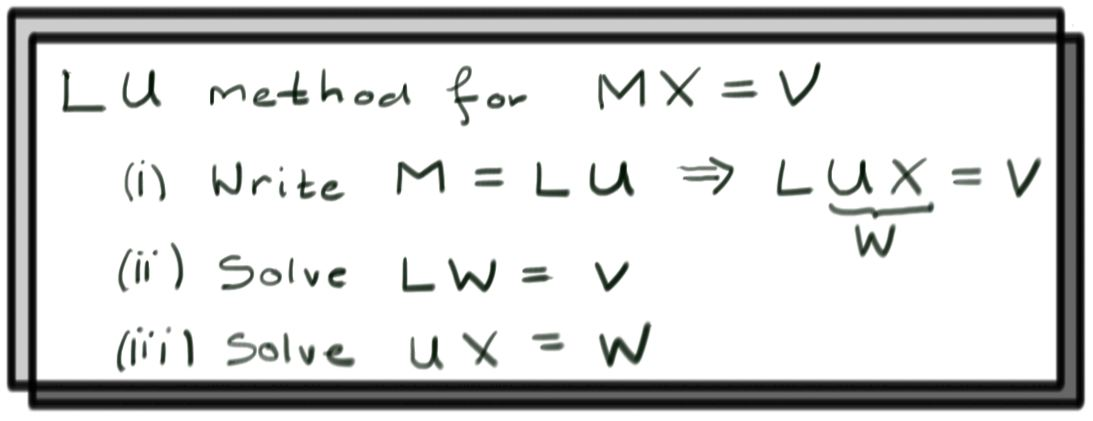
\includegraphics[scale=.3]{\luDecompPath/LU_solution.jpg}
\end{center}
%\end{figure}

\section{Finding an $LU$ Decomposition.}
\label{finding_LU_decomp}
 
For any given matrix, there are actually many different $LU$ decompositions.  However, there is a unique $LU$ decomposition in which the $L$ matrix has ones on the diagonal. In that case $L$ is called a \emph{lower unit triangular matrix}\index{Lower unit triangular matrix}.

To find the $LU$ decomposition, we'll create two sequences of matrices $L_0, L_1, \ldots$ and $U_0, U_1, \ldots$ such that at each step, $L_iU_i=M$.  Each of the $L_i$ will be lower triangular, but only the last $U_i$ will be upper triangular.

Start by setting $L_0=I$ and $U_0=M$, because $L_0U_0=M$. A main concept of this calculation is captured by the following example:

\begin{example}
Consider $$E=\begin{pmatrix}1&0\\\lambda&1\end{pmatrix}\, ,\qquad M=\begin{pmatrix}a&b&c&\cdots\\d&e&f&\cdots\end{pmatrix}\, .$$
Lets compute $EM$
$$
EM=\begin{pmatrix}a&b&c&\cdots\\d+\lambda a&e+\lambda b&f+\lambda c&\cdots\end{pmatrix}\, ,.
$$
Something neat happened here: multiplying $M$ by $E$ performed the row operation $R_2\to R_2+\lambda R-1$ on $M$.
Another interesting fact:
$$
E^{-1}:=\begin{pmatrix}1&0\\-\lambda&1\end{pmatrix}
$$ 
obeys (check this yourself...)
$$
E^{-1} E = 1\, .
$$
Hence $M=E^{-1} E M$ or, writing this out
$$
\begin{pmatrix}a&b&c&\cdots\\d&e&f&\cdots\end{pmatrix}=\begin{pmatrix}1&0\\-\lambda&1\end{pmatrix} \begin{pmatrix}a&b&c&\cdots\\d+\lambda a&e+\lambda b&f+\lambda c&\cdots\end{pmatrix}\, .
$$
Here the matrix on the left is lower triangular, while the matrix on the right has had a row operation performed on it.
\end{example}




\vspace{2mm}
We would like to  use the first row of $U_0$ to zero out the first entry of every row below it.  For our running example, $$U_0=M=\begin{pmatrix}
6 & 18 & 3 \\
2 & 12 & 1 \\
4 & 15 & 3 
\end{pmatrix}\, ,$$ so we would like to perform the row operations $R_2\to R_2 -\frac 13 R_1$ and $R_3\to R_3-\frac 23R_1$.
%so the second row minus $\frac{1}{3}$ of the first row will zero out the first entry in the second row.  Likewise, the third row minus $\frac{2}{3}$ of the first row will zero out the first entry in the third row.
If we perform these row operations on $U_0$ to produce 
$$U_1=\begin{pmatrix}
6 & 18 & 3 \\
0 & 6 & 0 \\
0 & 3 & 1 
\end{pmatrix}\, ,$$
we need to multiply this on the left by a lower triangular matrix $L_1$ so that the product $L_1U_1=M$ still.
The above example shows how to do this:
Set $L_1$ to be the lower triangular matrix whose first column is filled with the minus constants used to zero out the first column of $M$.  Then $$L_1 = \begin{pmatrix}
1 & 0 & 0 \\[1mm]
\frac{1}{3} & 1 & 0 \\[1mm]
\frac{2}{3} & 0 & 1 
\end{pmatrix}\, .$$  
%Set $U_1$ to be the matrix obtained by zeroing out the first column of $M$.  Then $U_1=\begin{pmatrix}
%6 & 18 & 3 \\
%0 & 6 & 0 \\
%0 & 3 & 1 
%\end{pmatrix}$.
By construction $L_1 U_1=M$, but you should compute this yourself as a double check.

Now repeat the process by zeroing the second column of $U_1$ below the diagonal using the second row of $U_1$ using the row operation
$R_3\to R_3-\frac 12 R_2$ to produce
$$U_2=\begin{pmatrix}6&18&3\\0&6&0\\0&0&1\end{pmatrix}\, .$$
The matrix that undoes this row operation is obtained in the same way we found $L_1$ above and is:
$$
\begin{pmatrix}
1&0&0\\
0&1&0\\
0&\frac 12& 0
\end{pmatrix}\, .
$$
Thus our answer for $L_2$ is the product of this matrix with $L_1$, namely
$$
L_2=
\begin{pmatrix}
1 & 0 & 0 \\[1mm]
\frac{1}{3} & 1 & 0 \\[1mm]
\frac{2}{3} & 0 & 1 
\end{pmatrix}\begin{pmatrix}
1&0&0\\
0&1&0\\
0&\frac 12& 0
\end{pmatrix}
=\begin{pmatrix}
1 & 0 & 0 \\[1mm]
\frac{1}{3} & 1 & 0 \\[1mm]
\frac{2}{3} & \frac{1}{2} & 1 
\end{pmatrix}\, .
$$
Notice that it is lower triangular because 

\begin{center}
\textcolor{brown}{THE PRODUCT OF LOWER TRIANGULAR MATRICES IS ALWAYS LOWER TRIANGULAR!}
\end{center}

\noindent
Moreover it is obtained by recording minus the constants used for all our row operations in the appropriate columns (this always works this way).
Moreover, $U_2$ is upper triangular and $M=L_2U_2$, we are done!
Putting this all together we have
$$M=\begin{pmatrix}
6 & 18 & 3 \\
2 & 12 & 1 \\
4 & 15 & 3 
\end{pmatrix}= \begin{pmatrix}
1 & 0 & 0 \\[1mm]
\frac{1}{3} & 1 & 0 \\[1mm]
\frac{2}{3} & \frac{1}{2} & 1 
\end{pmatrix}\begin{pmatrix}
6 & 18 & 3 \\
0 & 6 & 0 \\
0 & 0 & 1 
\end{pmatrix}\, .$$  
%Since $U_2$ is upper-triangular, we're done.  Inserting the new number into $L_1$ to get $L_2$ really is safe: the numbers in the first column don't affect the second column of $U_1$, since the first column of $U_1$ is already zeroed out.

If the matrix you're working with has more than three rows, just continue this process by zeroing out the next column below the diagonal, and repeat until there's nothing left to do.

\videoscriptlink{lu_decomposition_example.mp4}{Another $LU$ decomposition example}{scripts_lu_decomposition_example}

The fractions in the $L$ matrix are admittedly ugly.  For two matrices $LU$, we can multiply one entire column of $L$ by a constant $\lambda$ and divide the corresponding row of $U$ by the same constant without changing the product of the two matrices.  Then:

\begin{eqnarray*}
LU &=& \begin{pmatrix}
1 & 0 & 0 \\[1mm]
\frac{1}{3} & 1 & 0 \\[1mm]
\frac{2}{3} & \frac{1}{2} & 1 
\end{pmatrix}
I
\begin{pmatrix}
6 & 18 & 3 \\
0 & 6 & 0 \\
0 & 0 & 1 
\end{pmatrix} \\
&=&
\begin{pmatrix}
1 & 0 & 0 \\[1mm]
\frac{1}{3} & 1 & 0 \\[1mm]
\frac{2}{3} & \frac{1}{2} & 1 
\end{pmatrix}
\begin{pmatrix}
3 & 0 & 0 \\
0 & 6 & 0 \\
0 & 0 & 1 
\end{pmatrix}
\begin{pmatrix}
\frac{1}{3} & 0 & 0 \\[1mm]
0 & \frac{1}{6} & 0 \\[1mm]
0 & 0 & 1 
\end{pmatrix}
\begin{pmatrix}
6 & 18 & 3 \\
0 & 6 & 0 \\
0 & 0 & 1 
\end{pmatrix} \\
&=&
\begin{pmatrix}
3 & 0 & 0 \\
1 & 6 & 0 \\
2 & 3 & 1 
\end{pmatrix}\begin{pmatrix}
2 & 6 & 1 \\
0 & 1 & 0 \\
0 & 0 & 1 
\end{pmatrix}.
\end{eqnarray*}
The resulting matrix looks nicer, but isn't in standard (lower unit triangular matrix) form.

\reading{11}{2}
%\href{\webworkurl ReadingHomework11/2/}{Reading homework: problem 11.2}

For matrices that are not square, $LU$ decomposition still makes sense.  Given an $m\times n$ matrix $M$, for example we could write $M=LU$ with $L$ a square lower unit triangular matrix, and $U$ a rectangular matrix.  Then $L$ will be an $m\times m$ matrix, and $U$ will be an $m\times n$ matrix (of the same shape as $M$).  From here, the process is exactly the same as for a square matrix.  We create a sequence of matrices $L_i$ and $U_i$ that is eventually the $LU$ decomposition.  Again, we start with $L_0=I$ and $U_0=M$.

\begin{example}
Let's find the $LU$ decomposition of $M=U_0=\begin{pmatrix}
-2 & 1 & 3 \\
-4 & 4 & 1 
\end{pmatrix}$.  Since $M$ is a $2\times 3$ matrix, our decomposition will consist of a $2\times 2$ matrix and a $2\times 3$ matrix.  Then we start with $L_0=I_2=\begin{pmatrix}
1 & 0 \\
0 & 1
\end{pmatrix}$.

The next step is to zero-out the first column of $M$ below the diagonal.  There is only one row to cancel, then, and it can be removed by subtracting $2$ times the first row of $M$ to the second row of $M$.  Then:

\[
L_1=\begin{pmatrix}
1 & 0 \\
2 & 1
\end{pmatrix}, \qquad 
U_1 = \begin{pmatrix}
-2 & 1 & 3 \\
0 & 2 & -5 
\end{pmatrix}
\]
Since $U_1$ is upper triangular, we're done.  With a larger matrix, we would just continue the process.
\end{example}





\section{Block $LDU$ Decomposition}

Let $M$ be a square block matrix with square blocks $X,Y,Z,W$ such that $X^{-1}$ exists.  Then $M$ can be decomposed as a block $LDU$ decomposition, where $D$ is block diagonal, as follows:
\[
M=\begin{pmatrix}
X & Y \\
Z & W
\end{pmatrix}
\]

Then: \[M=\begin{pmatrix}
I &  0 \\
ZX^{-1} & I
\end{pmatrix}\begin{pmatrix}
X & 0 \\
0 & W-ZX^{-1}Y
\end{pmatrix}\begin{pmatrix}
I & X^{-1}Y \\
0 & I
\end{pmatrix}.\]
This can be checked explicitly simply by block-multiplying these three matrices.

\videoscriptlink{lu_decomposition_blocks.mp4}{Block $LDU$ Explanation}{scripts_lu_decomposition_blocks}

\begin{example}
For a $2\times 2$ matrix, we can regard each entry as a block.
\[
\begin{pmatrix}
1 & 2 \\
3 & 4
\end{pmatrix}=
\begin{pmatrix}
1 & 0 \\
3 & 1
\end{pmatrix}
\begin{pmatrix}
1 & 0 \\
0 & -2
\end{pmatrix}
\begin{pmatrix}
1 & 2 \\
0 & 1
\end{pmatrix}
\]
By multiplying the diagonal matrix by the upper triangular matrix, we get the standard $LU$ decomposition of the matrix.
\end{example}


%\section*{References}
%Wikipedia:
%\begin{itemize}
%\item \href{http://en.wikipedia.org/wiki/LU_decomposition}{$LU$ Decomposition}
%\item \href{http://en.wikipedia.org/wiki/Block_LU_decomposition}{Block $LU$ Decomposition}
%\end{itemize}

\section{Review Problems}



\begin{enumerate}

\item Let $D=\begin{pmatrix}
\lambda_1 & \mc0 \\
\mc0 & \lambda_2 \\
\end{pmatrix}$.
\begin{enumerate}
\item Write $D$ in terms of the vectors $e_1$ and $e_2$, and their transposes.
\item Suppose $P=\begin{pmatrix}
a & b \\
c & d \\
\end{pmatrix}$ is invertible.  Show that $D$ is similar to
\[
M=\frac{1}{ad-bc}\begin{pmatrix}
\lambda_1ad-\lambda_2bc & -(\lambda_1-\lambda_2)ab \\[1mm]
(\lambda_1-\lambda_2)cd & -\lambda_1bc + \lambda_2ad
\end{pmatrix}.
\]
\item Suppose the vectors $\rowvec{a,b}$ and $\rowvec{c,d}$ are orthogonal.  What can you say about $M$ in this case? (Hint: think about what \(M^T\) is equal to.)
\end{enumerate}

\phantomnewpage

\item \label{orthogprob} Suppose $S=\{v_1, \ldots, v_n \}$ is an \emph{orthogonal} (not orthonormal) basis for~$\Re^n$.  Then we can write any vector $v$ as $v=\sum_ic^iv_i$ for some constants $c^i$.  Find a formula for the constants $c^i$ in terms of $v$ and the vectors in~$S$.

\Videoscriptlink{orthonormal_bases_hint.mp4}{Hint}{scripts_orthonormal_bases_hint}
\phantomnewpage

\item \label{orthogprojprob} Let $u,v$ be linearly independent vectors in $\Re^3$, and $P=\spa \{ u,v\}$ be the plane spanned by $u$ and $v$.  
\begin{enumerate}
\item Is the vector $v^\bot := v-\frac{u\cdot v}{u\cdot u}u$ in the plane $P$?
\item  What is the (cosine of the) angle between $v^\bot$ and $u$?
\item %Given your solution to the above, 
How can you find a third vector perpendicular to both $u$ and $v^\bot$?
\item  Construct an orthonormal basis for $\Re^3$ from $u$ and $v$.
\item  Test your abstract formul\ae\ starting with 
\[
u=\rowvec{1 , 2 , 0} \text{ and } v=\rowvec{0 , 1 , 1}.
\]
\end{enumerate}

\Videoscriptlink{orthonormal_bases_hint3.mp4}{Hint}{scripts_orthonormal_bases_hint3}

\phantomnewpage



\item Find an orthonormal  basis for $\Re^4$ which includes $(1,1,1,1)$ using the following procedure:\\
\begin{enumerate} 
\item Pick a vector perpendicular to the vector 
$$v_1 =\colvec{1\\1\\1\\1}$$ from the solution set of the matrix equation $$v_1^Tx=0\, .$$ Pick the vector $v_2$ obtained from the standard Gaussian elimination procedure which is the coefficient of $x_2$.
\item Pick a vector perpendicular to both $v_1$ and $v_2$ from the solutions set of the matrix equation $$\colvec{v_1^T\\[1mm]v_2^T}x=0\, .$$ Pick the vector $v_3$ obtained from the standard Gaussian elimination procedure with $x_3$ as the coefficient. 
\item Pick a vector perpendicular to $v_1,v_2,$ and $v_3$ from the solution set of the matrix equation $$\colvec{v_1^T\\[1mm]v_2^T\\[1mm]v_3^T}x=0\, .$$  Pick the vector $v_4$ obtained from the standard Gaussian elimination procedure with $x_3$ as the coefficient. 
\item Normalize the four vectors obtained   above.
\end{enumerate}


\item Use the inner product $$f\cdot g := \int_0^1 f(x)g(x)dx$$  on the vector space $V={\rm span} \{1,x,x^2,x^3\}$ to perform the Gram-Schmidt procedure on the set of vectors $\{1,x,x^2,x^3\}$. 

\item Use the inner product $$f\cdot g := \int_0^{2\pi} f(x)g(x)dx$$  on the vector space $V={\rm span} \{\sin(x),\sin(2x),\sin(3x) \}$ to perform the Gram-Schmidt procedure on the set of vectors $\{\sin(x),\sin(2x),\sin(3x) \}$. \\
Try to build an orthonormal basis for the vector space $$\spa \{ \sin(nx)~| ~n\in \N \}\, .$$
%What do you suspect about the vector space $\spa \{ \sin(nx)~| ~n\in \N \}$?\\
%What do you suspect about the vector space $\spa \{ \sin(ax)~|~ a \in \Re \}$?
\item 
\begin{enumerate}
\item
Show that if $Q$ is an orthogonal $n\times n$ matrix, then $$u\dotprod v = (Qu)\dotprod (Qv)\, ,$$ for any $u,v\in \Re^n$. That is, $Q$ preserves the inner product. 
\item Does $Q$ preserve the outer product? 
\item  If the set of vectors $\{ u_1,\dots,u_n\}$ is orthonormal and $\{ \lambda_1,\cdots,\lambda_n\}$ is a set of numbers, 
then what are the eigenvalues and eigenvectors of the matrix
$M=\sum_{i=1}^n \lambda_i u_i u_i^T$? 
\item How would the eigenvectors and eigenvalues of this matrix change if we replaced  $\{ u_1,\dots,u_n\}$ by $\{ Qu_1,\dots,Q u_n\}$?
\end{enumerate}


\item Carefully write out the Gram-Schmidt procedure for the set of vectors 
$$\left\{ \colvec{1\\1\\1}, \colvec{1\\-1\\1}, \colvec{1\\1\\-1} \right\} \, .$$ Is it possible to rescale the second vector obtained in the procedure to a vector with integer components? 


\item 
\label{basisortho}
\begin{enumerate}
\item Suppose $u$ and $v$ are linearly independent.  Show that $u$ and $v^\perp$ are also linearly independent.  Explain why $\{u, v^\perp\}$ is a basis for $\spa \{u,v\}$.



\Videoscriptlink{gram_schmidt_and_orthogonal_complements_hint.mp4}{Hint}{gram_schmidt_and_orthogonal_complements_hint}

\item Repeat the previous problem, but with three independent vectors $u,v,w$
 where $v^\perp$ and $w^\perp$ are as defined by the Gram-Schmidt procedure. 
\end{enumerate}

\phantomnewpage


\item \label{QRprob} Find the $QR$ factorization of
$$
M=\begin{pmatrix}1&0&\phantom{\!-}2\\-1&2&0\\-1&-2&2
\end{pmatrix}\, .
$$

\phantomnewpage

\item Given any three vectors $u,v,w$, when do $v^\perp$ or $w^\perp$ of the Gram--Schmidt procedure vanish?

\phantomnewpage

\item For $U$ a subspace of $W$, use the subspace theorem to check that $U^\perp$ is a subspace of $W$.

\phantomnewpage


\phantomnewpage

\item %(Extra Credit) 
Let $S_n$ and $A_n$ define the space of $n \times n$ symmetric and anti-symmetric matrices, respectively. These are subspaces of the vector space $M^n_n$ of all $n\times n$ matrices. What is $\dim M^n_n$, $\dim S_n$, and $\dim A_n$? Show that $M^n_n = S_n + A_n$. Define an inner product on square matrices
$$
M\cdot N ={\rm tr} MN\, .
$$
Is $A_n^{\perp}=S_n$? Is $M^n_n = S_n \oplus A_n$?

%\emph{Hint: Note that $\dim S_n = \dim U_n$ where $U_n$ is the vector space of all $n \times n$ upper triangular matrices, and also note that $\dim A_n = \dim \widetilde{U}_n$ where $\widetilde{U}_n$ is the vector space of all strictly $n \times n$ upper triangular matrices (\emph{i.e.} the diagonal entries are all 0).}

\item The vector space $V={\rm span} \{ \sin(t),\sin(2t), \sin(3t) , \sin(3t)\}$ has an inner product: 
$$f\cdot g:=\int _0^{2\pi}f(t)g(t) dt\, .$$ Find the orthogonal compliment to $U={\rm span} \{ \sin(t)+\sin(2t) \}$ in $V$. Express $\sin(t)-\sin(2t)$ as  the sum of vectors from $U$ and $U^\perp$.

\end{enumerate}

\phantomnewpage

\newpage
 %ch 12 w3

%\chapter{\luDecompTitle}
\label{LUdecomp}

Certain matrices are easier to work with than others.  In this section, we will see how to write any square\footnote{The case where $M$ is not square is dealt with at the end of the lecture.} matrix $M$ as the product of two simpler matrices.  We will write $$M=LU\, ,$$ where:
\begin{itemize}
\item $L$ is \emph{lower triangular}\index{Lower triangular matrix}.  This means that all entries above the main diagonal are zero.  In notation,
$L=(l^i_j)$ with $l^i_j=0$ for all $j>i$.
\[L=\begin{pmatrix}
l^1_1 & 0 & 0 & \cdots \\
l^2_1 & l^2_2 & 0 & \cdots \\
l^3_1 & l^3_2 & l^3_3 & \cdots \\
\vdots & \vdots & \vdots & \ddots \\
\end{pmatrix}
\]

\item $U$ is \emph{upper triangular}\index{Upper triangular matrix}.  This means that all entries below the main diagonal are zero.  In notation,
$U=(u^i_j)$ with $u^i_j=0$ for all $j<i$.
\[U=\begin{pmatrix}
u^1_1 & u^1_2 & u^1_3 & \cdots \\
0 & u^2_2 & u^2_3 & \cdots \\
0 & 0 & u^3_3 & \cdots \\
\vdots & \vdots & \vdots & \ddots \\
\end{pmatrix}
\]
\end{itemize}
$M=LU$ is called an \emph{$LU$ decomposition}\index{LU@$LU$ decomposition} of $M$.

This is a useful trick for  computational reasons; it is much easier to compute the inverse of an upper or lower triangular matrix than general matrices.  Since inverses are useful for solving linear systems, this makes solving any linear system associated to the matrix much faster as well.  The determinant---a very important quantity associated with any square matrix---is very easy to compute for triangular matrices.

\begin{example}
Linear systems associated to upper triangular matrices are very easy to solve by back substitution.
\[
\begin{amatrix}{2}
a & b & 1 \\
0 & c & e \\
\end{amatrix} \ \Rightarrow \ y=\frac{e}{c}\, , \quad x=\frac{1}{a}\left(1-\frac{be}{c}\right)
\]

\[
\begin{amatrix}{3}
1 & 0 & 0 & d \\
a & 1 & 0 & e \\
b & c & 1 & f \\
\end{amatrix} \Rightarrow x=d\, , \qquad y=e-ad\, , \qquad z=f-bd-c(e-ad)
\]
For lower triangular matrices, \emph{back} substitution\index{Back substitution} gives a quick solution; for upper triangular matrices, \emph{forward} substitution\index{Forward substitution} gives the solution.
\end{example}





\section{Using $LU$ Decomposition to Solve Linear Systems}

Suppose we have $M=LU$ and want to solve the system
\[
MX=LUX=V.
\]

\begin{itemize}
\item{Step 1:} Set $W=\colvec{u\\v\\w}=UX$.  

\item{Step 2:} Solve the system $LW=V$.  This should be simple by forward substitution since $L$ is lower triangular.  Suppose the solution to $LW=V$ is $W_0$.  

\item{Step 3:} Now solve the system $UX=W_0$.  This should be easy by backward substitution, since $U$ is upper triangular.  The solution to this system is the solution to the original system.
\end{itemize}
We can think of this as using the matrix $L$ to perform row operations on the matrix $U$ in order to solve the system; this idea also appears in the  study of determinants.

%\href{\webworkurl ReadingHomework11/1/}{Reading homework: problem 11.1}
\reading{11}{1}

\begin{example}
Consider the linear system:
\[
      \begin{linsys}{4}
            6x & +&18y & +&3z         &=& 3  \\[1mm]
            2x & +&12y & +&z	    &=& 19 \\[1mm]
            4x & +&15y & +&3z         &=& 0  
      \end{linsys}
\]

An $LU$ decomposition for the associated matrix $M$ is:
\[
\begin{pmatrix}
6 & 18 & 3 \\
2 & 12 & 1 \\
4 & 15 & 3 
\end{pmatrix} =
\begin{pmatrix}
3 & 0 & 0 \\
1 & 6 & 0 \\
2 & 3 & 1 
\end{pmatrix}
\begin{pmatrix}
2 & 6 & 1 \\
0 & 1 & 0 \\
0 & 0 & 1 
\end{pmatrix}.
\]

\begin{itemize}
\item{Step 1:} \hypertarget{LUproc}{Set} $W=\colvec{u\\v\\w}=UX$.  

\item{Step 2:} Solve the system $LW=V$:

\[
\begin{pmatrix}
3 & 0 & 0 \\
1 & 6 & 0 \\
2 & 3 & 1 
\end{pmatrix}
\colvec{u\\v\\w} =
\colvec{3\\19\\0}
\]

By substitution, we get $u=1$, $v=3$, and $w=-11$.  Then 
\[W_0=\colvec{1\\3\\-11}\]

\item{Step 3:} Solve the system $UX=W_0$.  
\[
\begin{pmatrix}
2 & 6 & 1 \\
0 & 1 & 0 \\
0 & 0 & 1 
\end{pmatrix}
\colvec{x\\y\\z} =
\colvec{1\\3\\-11}
\]
Back substitution gives $z=-11, y=3$, and $x=-3$.  

Then $X=\colvec{-3\\3\\-11}$, and we're done.
\end{itemize}
\end{example}

\videoscriptlink{lu_decomposition_using_lu_decomp.mp4}{Using a $LU$ decomposition}{scripts_lu_decomposition_using_lu_example}

%\begin{figure}
\begin{center}
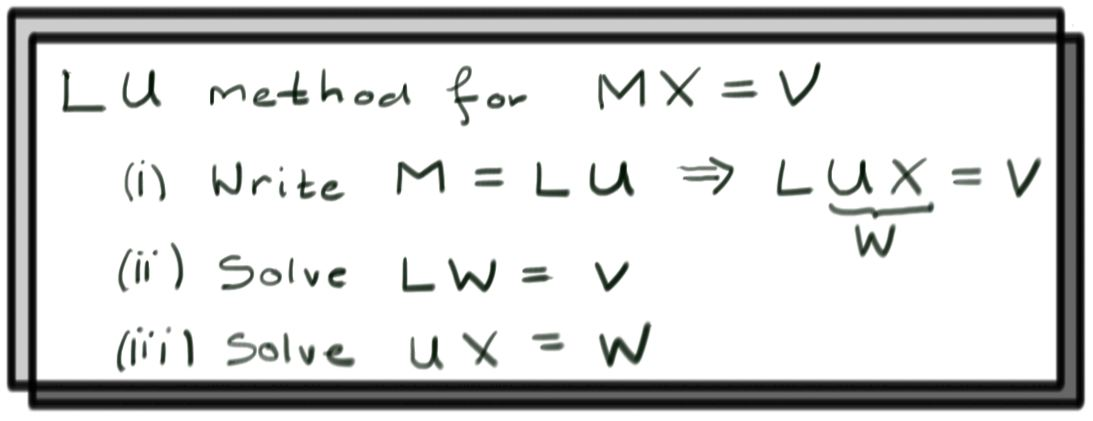
\includegraphics[scale=.3]{\luDecompPath/LU_solution.jpg}
\end{center}
%\end{figure}

\section{Finding an $LU$ Decomposition.}
\label{finding_LU_decomp}
 
For any given matrix, there are actually many different $LU$ decompositions.  However, there is a unique $LU$ decomposition in which the $L$ matrix has ones on the diagonal. In that case $L$ is called a \emph{lower unit triangular matrix}\index{Lower unit triangular matrix}.

To find the $LU$ decomposition, we'll create two sequences of matrices $L_0, L_1, \ldots$ and $U_0, U_1, \ldots$ such that at each step, $L_iU_i=M$.  Each of the $L_i$ will be lower triangular, but only the last $U_i$ will be upper triangular.

Start by setting $L_0=I$ and $U_0=M$, because $L_0U_0=M$. A main concept of this calculation is captured by the following example:

\begin{example}
Consider $$E=\begin{pmatrix}1&0\\\lambda&1\end{pmatrix}\, ,\qquad M=\begin{pmatrix}a&b&c&\cdots\\d&e&f&\cdots\end{pmatrix}\, .$$
Lets compute $EM$
$$
EM=\begin{pmatrix}a&b&c&\cdots\\d+\lambda a&e+\lambda b&f+\lambda c&\cdots\end{pmatrix}\, ,.
$$
Something neat happened here: multiplying $M$ by $E$ performed the row operation $R_2\to R_2+\lambda R-1$ on $M$.
Another interesting fact:
$$
E^{-1}:=\begin{pmatrix}1&0\\-\lambda&1\end{pmatrix}
$$ 
obeys (check this yourself...)
$$
E^{-1} E = 1\, .
$$
Hence $M=E^{-1} E M$ or, writing this out
$$
\begin{pmatrix}a&b&c&\cdots\\d&e&f&\cdots\end{pmatrix}=\begin{pmatrix}1&0\\-\lambda&1\end{pmatrix} \begin{pmatrix}a&b&c&\cdots\\d+\lambda a&e+\lambda b&f+\lambda c&\cdots\end{pmatrix}\, .
$$
Here the matrix on the left is lower triangular, while the matrix on the right has had a row operation performed on it.
\end{example}




\vspace{2mm}
We would like to  use the first row of $U_0$ to zero out the first entry of every row below it.  For our running example, $$U_0=M=\begin{pmatrix}
6 & 18 & 3 \\
2 & 12 & 1 \\
4 & 15 & 3 
\end{pmatrix}\, ,$$ so we would like to perform the row operations $R_2\to R_2 -\frac 13 R_1$ and $R_3\to R_3-\frac 23R_1$.
%so the second row minus $\frac{1}{3}$ of the first row will zero out the first entry in the second row.  Likewise, the third row minus $\frac{2}{3}$ of the first row will zero out the first entry in the third row.
If we perform these row operations on $U_0$ to produce 
$$U_1=\begin{pmatrix}
6 & 18 & 3 \\
0 & 6 & 0 \\
0 & 3 & 1 
\end{pmatrix}\, ,$$
we need to multiply this on the left by a lower triangular matrix $L_1$ so that the product $L_1U_1=M$ still.
The above example shows how to do this:
Set $L_1$ to be the lower triangular matrix whose first column is filled with the minus constants used to zero out the first column of $M$.  Then $$L_1 = \begin{pmatrix}
1 & 0 & 0 \\[1mm]
\frac{1}{3} & 1 & 0 \\[1mm]
\frac{2}{3} & 0 & 1 
\end{pmatrix}\, .$$  
%Set $U_1$ to be the matrix obtained by zeroing out the first column of $M$.  Then $U_1=\begin{pmatrix}
%6 & 18 & 3 \\
%0 & 6 & 0 \\
%0 & 3 & 1 
%\end{pmatrix}$.
By construction $L_1 U_1=M$, but you should compute this yourself as a double check.

Now repeat the process by zeroing the second column of $U_1$ below the diagonal using the second row of $U_1$ using the row operation
$R_3\to R_3-\frac 12 R_2$ to produce
$$U_2=\begin{pmatrix}6&18&3\\0&6&0\\0&0&1\end{pmatrix}\, .$$
The matrix that undoes this row operation is obtained in the same way we found $L_1$ above and is:
$$
\begin{pmatrix}
1&0&0\\
0&1&0\\
0&\frac 12& 0
\end{pmatrix}\, .
$$
Thus our answer for $L_2$ is the product of this matrix with $L_1$, namely
$$
L_2=
\begin{pmatrix}
1 & 0 & 0 \\[1mm]
\frac{1}{3} & 1 & 0 \\[1mm]
\frac{2}{3} & 0 & 1 
\end{pmatrix}\begin{pmatrix}
1&0&0\\
0&1&0\\
0&\frac 12& 0
\end{pmatrix}
=\begin{pmatrix}
1 & 0 & 0 \\[1mm]
\frac{1}{3} & 1 & 0 \\[1mm]
\frac{2}{3} & \frac{1}{2} & 1 
\end{pmatrix}\, .
$$
Notice that it is lower triangular because 

\begin{center}
\textcolor{brown}{THE PRODUCT OF LOWER TRIANGULAR MATRICES IS ALWAYS LOWER TRIANGULAR!}
\end{center}

\noindent
Moreover it is obtained by recording minus the constants used for all our row operations in the appropriate columns (this always works this way).
Moreover, $U_2$ is upper triangular and $M=L_2U_2$, we are done!
Putting this all together we have
$$M=\begin{pmatrix}
6 & 18 & 3 \\
2 & 12 & 1 \\
4 & 15 & 3 
\end{pmatrix}= \begin{pmatrix}
1 & 0 & 0 \\[1mm]
\frac{1}{3} & 1 & 0 \\[1mm]
\frac{2}{3} & \frac{1}{2} & 1 
\end{pmatrix}\begin{pmatrix}
6 & 18 & 3 \\
0 & 6 & 0 \\
0 & 0 & 1 
\end{pmatrix}\, .$$  
%Since $U_2$ is upper-triangular, we're done.  Inserting the new number into $L_1$ to get $L_2$ really is safe: the numbers in the first column don't affect the second column of $U_1$, since the first column of $U_1$ is already zeroed out.

If the matrix you're working with has more than three rows, just continue this process by zeroing out the next column below the diagonal, and repeat until there's nothing left to do.

\videoscriptlink{lu_decomposition_example.mp4}{Another $LU$ decomposition example}{scripts_lu_decomposition_example}

The fractions in the $L$ matrix are admittedly ugly.  For two matrices $LU$, we can multiply one entire column of $L$ by a constant $\lambda$ and divide the corresponding row of $U$ by the same constant without changing the product of the two matrices.  Then:

\begin{eqnarray*}
LU &=& \begin{pmatrix}
1 & 0 & 0 \\[1mm]
\frac{1}{3} & 1 & 0 \\[1mm]
\frac{2}{3} & \frac{1}{2} & 1 
\end{pmatrix}
I
\begin{pmatrix}
6 & 18 & 3 \\
0 & 6 & 0 \\
0 & 0 & 1 
\end{pmatrix} \\
&=&
\begin{pmatrix}
1 & 0 & 0 \\[1mm]
\frac{1}{3} & 1 & 0 \\[1mm]
\frac{2}{3} & \frac{1}{2} & 1 
\end{pmatrix}
\begin{pmatrix}
3 & 0 & 0 \\
0 & 6 & 0 \\
0 & 0 & 1 
\end{pmatrix}
\begin{pmatrix}
\frac{1}{3} & 0 & 0 \\[1mm]
0 & \frac{1}{6} & 0 \\[1mm]
0 & 0 & 1 
\end{pmatrix}
\begin{pmatrix}
6 & 18 & 3 \\
0 & 6 & 0 \\
0 & 0 & 1 
\end{pmatrix} \\
&=&
\begin{pmatrix}
3 & 0 & 0 \\
1 & 6 & 0 \\
2 & 3 & 1 
\end{pmatrix}\begin{pmatrix}
2 & 6 & 1 \\
0 & 1 & 0 \\
0 & 0 & 1 
\end{pmatrix}.
\end{eqnarray*}
The resulting matrix looks nicer, but isn't in standard (lower unit triangular matrix) form.

\reading{11}{2}
%\href{\webworkurl ReadingHomework11/2/}{Reading homework: problem 11.2}

For matrices that are not square, $LU$ decomposition still makes sense.  Given an $m\times n$ matrix $M$, for example we could write $M=LU$ with $L$ a square lower unit triangular matrix, and $U$ a rectangular matrix.  Then $L$ will be an $m\times m$ matrix, and $U$ will be an $m\times n$ matrix (of the same shape as $M$).  From here, the process is exactly the same as for a square matrix.  We create a sequence of matrices $L_i$ and $U_i$ that is eventually the $LU$ decomposition.  Again, we start with $L_0=I$ and $U_0=M$.

\begin{example}
Let's find the $LU$ decomposition of $M=U_0=\begin{pmatrix}
-2 & 1 & 3 \\
-4 & 4 & 1 
\end{pmatrix}$.  Since $M$ is a $2\times 3$ matrix, our decomposition will consist of a $2\times 2$ matrix and a $2\times 3$ matrix.  Then we start with $L_0=I_2=\begin{pmatrix}
1 & 0 \\
0 & 1
\end{pmatrix}$.

The next step is to zero-out the first column of $M$ below the diagonal.  There is only one row to cancel, then, and it can be removed by subtracting $2$ times the first row of $M$ to the second row of $M$.  Then:

\[
L_1=\begin{pmatrix}
1 & 0 \\
2 & 1
\end{pmatrix}, \qquad 
U_1 = \begin{pmatrix}
-2 & 1 & 3 \\
0 & 2 & -5 
\end{pmatrix}
\]
Since $U_1$ is upper triangular, we're done.  With a larger matrix, we would just continue the process.
\end{example}





\section{Block $LDU$ Decomposition}

Let $M$ be a square block matrix with square blocks $X,Y,Z,W$ such that $X^{-1}$ exists.  Then $M$ can be decomposed as a block $LDU$ decomposition, where $D$ is block diagonal, as follows:
\[
M=\begin{pmatrix}
X & Y \\
Z & W
\end{pmatrix}
\]

Then: \[M=\begin{pmatrix}
I &  0 \\
ZX^{-1} & I
\end{pmatrix}\begin{pmatrix}
X & 0 \\
0 & W-ZX^{-1}Y
\end{pmatrix}\begin{pmatrix}
I & X^{-1}Y \\
0 & I
\end{pmatrix}.\]
This can be checked explicitly simply by block-multiplying these three matrices.

\videoscriptlink{lu_decomposition_blocks.mp4}{Block $LDU$ Explanation}{scripts_lu_decomposition_blocks}

\begin{example}
For a $2\times 2$ matrix, we can regard each entry as a block.
\[
\begin{pmatrix}
1 & 2 \\
3 & 4
\end{pmatrix}=
\begin{pmatrix}
1 & 0 \\
3 & 1
\end{pmatrix}
\begin{pmatrix}
1 & 0 \\
0 & -2
\end{pmatrix}
\begin{pmatrix}
1 & 2 \\
0 & 1
\end{pmatrix}
\]
By multiplying the diagonal matrix by the upper triangular matrix, we get the standard $LU$ decomposition of the matrix.
\end{example}


%\section*{References}
%Wikipedia:
%\begin{itemize}
%\item \href{http://en.wikipedia.org/wiki/LU_decomposition}{$LU$ Decomposition}
%\item \href{http://en.wikipedia.org/wiki/Block_LU_decomposition}{Block $LU$ Decomposition}
%\end{itemize}

\section{Review Problems}



\begin{enumerate}

\item Let $D=\begin{pmatrix}
\lambda_1 & \mc0 \\
\mc0 & \lambda_2 \\
\end{pmatrix}$.
\begin{enumerate}
\item Write $D$ in terms of the vectors $e_1$ and $e_2$, and their transposes.
\item Suppose $P=\begin{pmatrix}
a & b \\
c & d \\
\end{pmatrix}$ is invertible.  Show that $D$ is similar to
\[
M=\frac{1}{ad-bc}\begin{pmatrix}
\lambda_1ad-\lambda_2bc & -(\lambda_1-\lambda_2)ab \\[1mm]
(\lambda_1-\lambda_2)cd & -\lambda_1bc + \lambda_2ad
\end{pmatrix}.
\]
\item Suppose the vectors $\rowvec{a,b}$ and $\rowvec{c,d}$ are orthogonal.  What can you say about $M$ in this case? (Hint: think about what \(M^T\) is equal to.)
\end{enumerate}

\phantomnewpage

\item \label{orthogprob} Suppose $S=\{v_1, \ldots, v_n \}$ is an \emph{orthogonal} (not orthonormal) basis for~$\Re^n$.  Then we can write any vector $v$ as $v=\sum_ic^iv_i$ for some constants $c^i$.  Find a formula for the constants $c^i$ in terms of $v$ and the vectors in~$S$.

\Videoscriptlink{orthonormal_bases_hint.mp4}{Hint}{scripts_orthonormal_bases_hint}
\phantomnewpage

\item \label{orthogprojprob} Let $u,v$ be linearly independent vectors in $\Re^3$, and $P=\spa \{ u,v\}$ be the plane spanned by $u$ and $v$.  
\begin{enumerate}
\item Is the vector $v^\bot := v-\frac{u\cdot v}{u\cdot u}u$ in the plane $P$?
\item  What is the (cosine of the) angle between $v^\bot$ and $u$?
\item %Given your solution to the above, 
How can you find a third vector perpendicular to both $u$ and $v^\bot$?
\item  Construct an orthonormal basis for $\Re^3$ from $u$ and $v$.
\item  Test your abstract formul\ae\ starting with 
\[
u=\rowvec{1 , 2 , 0} \text{ and } v=\rowvec{0 , 1 , 1}.
\]
\end{enumerate}

\Videoscriptlink{orthonormal_bases_hint3.mp4}{Hint}{scripts_orthonormal_bases_hint3}

\phantomnewpage



\item Find an orthonormal  basis for $\Re^4$ which includes $(1,1,1,1)$ using the following procedure:\\
\begin{enumerate} 
\item Pick a vector perpendicular to the vector 
$$v_1 =\colvec{1\\1\\1\\1}$$ from the solution set of the matrix equation $$v_1^Tx=0\, .$$ Pick the vector $v_2$ obtained from the standard Gaussian elimination procedure which is the coefficient of $x_2$.
\item Pick a vector perpendicular to both $v_1$ and $v_2$ from the solutions set of the matrix equation $$\colvec{v_1^T\\[1mm]v_2^T}x=0\, .$$ Pick the vector $v_3$ obtained from the standard Gaussian elimination procedure with $x_3$ as the coefficient. 
\item Pick a vector perpendicular to $v_1,v_2,$ and $v_3$ from the solution set of the matrix equation $$\colvec{v_1^T\\[1mm]v_2^T\\[1mm]v_3^T}x=0\, .$$  Pick the vector $v_4$ obtained from the standard Gaussian elimination procedure with $x_3$ as the coefficient. 
\item Normalize the four vectors obtained   above.
\end{enumerate}


\item Use the inner product $$f\cdot g := \int_0^1 f(x)g(x)dx$$  on the vector space $V={\rm span} \{1,x,x^2,x^3\}$ to perform the Gram-Schmidt procedure on the set of vectors $\{1,x,x^2,x^3\}$. 

\item Use the inner product $$f\cdot g := \int_0^{2\pi} f(x)g(x)dx$$  on the vector space $V={\rm span} \{\sin(x),\sin(2x),\sin(3x) \}$ to perform the Gram-Schmidt procedure on the set of vectors $\{\sin(x),\sin(2x),\sin(3x) \}$. \\
Try to build an orthonormal basis for the vector space $$\spa \{ \sin(nx)~| ~n\in \N \}\, .$$
%What do you suspect about the vector space $\spa \{ \sin(nx)~| ~n\in \N \}$?\\
%What do you suspect about the vector space $\spa \{ \sin(ax)~|~ a \in \Re \}$?
\item 
\begin{enumerate}
\item
Show that if $Q$ is an orthogonal $n\times n$ matrix, then $$u\dotprod v = (Qu)\dotprod (Qv)\, ,$$ for any $u,v\in \Re^n$. That is, $Q$ preserves the inner product. 
\item Does $Q$ preserve the outer product? 
\item  If the set of vectors $\{ u_1,\dots,u_n\}$ is orthonormal and $\{ \lambda_1,\cdots,\lambda_n\}$ is a set of numbers, 
then what are the eigenvalues and eigenvectors of the matrix
$M=\sum_{i=1}^n \lambda_i u_i u_i^T$? 
\item How would the eigenvectors and eigenvalues of this matrix change if we replaced  $\{ u_1,\dots,u_n\}$ by $\{ Qu_1,\dots,Q u_n\}$?
\end{enumerate}


\item Carefully write out the Gram-Schmidt procedure for the set of vectors 
$$\left\{ \colvec{1\\1\\1}, \colvec{1\\-1\\1}, \colvec{1\\1\\-1} \right\} \, .$$ Is it possible to rescale the second vector obtained in the procedure to a vector with integer components? 


\item 
\label{basisortho}
\begin{enumerate}
\item Suppose $u$ and $v$ are linearly independent.  Show that $u$ and $v^\perp$ are also linearly independent.  Explain why $\{u, v^\perp\}$ is a basis for $\spa \{u,v\}$.



\Videoscriptlink{gram_schmidt_and_orthogonal_complements_hint.mp4}{Hint}{gram_schmidt_and_orthogonal_complements_hint}

\item Repeat the previous problem, but with three independent vectors $u,v,w$
 where $v^\perp$ and $w^\perp$ are as defined by the Gram-Schmidt procedure. 
\end{enumerate}

\phantomnewpage


\item \label{QRprob} Find the $QR$ factorization of
$$
M=\begin{pmatrix}1&0&\phantom{\!-}2\\-1&2&0\\-1&-2&2
\end{pmatrix}\, .
$$

\phantomnewpage

\item Given any three vectors $u,v,w$, when do $v^\perp$ or $w^\perp$ of the Gram--Schmidt procedure vanish?

\phantomnewpage

\item For $U$ a subspace of $W$, use the subspace theorem to check that $U^\perp$ is a subspace of $W$.

\phantomnewpage


\phantomnewpage

\item %(Extra Credit) 
Let $S_n$ and $A_n$ define the space of $n \times n$ symmetric and anti-symmetric matrices, respectively. These are subspaces of the vector space $M^n_n$ of all $n\times n$ matrices. What is $\dim M^n_n$, $\dim S_n$, and $\dim A_n$? Show that $M^n_n = S_n + A_n$. Define an inner product on square matrices
$$
M\cdot N ={\rm tr} MN\, .
$$
Is $A_n^{\perp}=S_n$? Is $M^n_n = S_n \oplus A_n$?

%\emph{Hint: Note that $\dim S_n = \dim U_n$ where $U_n$ is the vector space of all $n \times n$ upper triangular matrices, and also note that $\dim A_n = \dim \widetilde{U}_n$ where $\widetilde{U}_n$ is the vector space of all strictly $n \times n$ upper triangular matrices (\emph{i.e.} the diagonal entries are all 0).}

\item The vector space $V={\rm span} \{ \sin(t),\sin(2t), \sin(3t) , \sin(3t)\}$ has an inner product: 
$$f\cdot g:=\int _0^{2\pi}f(t)g(t) dt\, .$$ Find the orthogonal compliment to $U={\rm span} \{ \sin(t)+\sin(2t) \}$ in $V$. Express $\sin(t)-\sin(2t)$ as  the sum of vectors from $U$ and $U^\perp$.

\end{enumerate}

\phantomnewpage

\newpage
 

%\chapter{\luDecompTitle}
\label{LUdecomp}

Certain matrices are easier to work with than others.  In this section, we will see how to write any square\footnote{The case where $M$ is not square is dealt with at the end of the lecture.} matrix $M$ as the product of two simpler matrices.  We will write $$M=LU\, ,$$ where:
\begin{itemize}
\item $L$ is \emph{lower triangular}\index{Lower triangular matrix}.  This means that all entries above the main diagonal are zero.  In notation,
$L=(l^i_j)$ with $l^i_j=0$ for all $j>i$.
\[L=\begin{pmatrix}
l^1_1 & 0 & 0 & \cdots \\
l^2_1 & l^2_2 & 0 & \cdots \\
l^3_1 & l^3_2 & l^3_3 & \cdots \\
\vdots & \vdots & \vdots & \ddots \\
\end{pmatrix}
\]

\item $U$ is \emph{upper triangular}\index{Upper triangular matrix}.  This means that all entries below the main diagonal are zero.  In notation,
$U=(u^i_j)$ with $u^i_j=0$ for all $j<i$.
\[U=\begin{pmatrix}
u^1_1 & u^1_2 & u^1_3 & \cdots \\
0 & u^2_2 & u^2_3 & \cdots \\
0 & 0 & u^3_3 & \cdots \\
\vdots & \vdots & \vdots & \ddots \\
\end{pmatrix}
\]
\end{itemize}
$M=LU$ is called an \emph{$LU$ decomposition}\index{LU@$LU$ decomposition} of $M$.

This is a useful trick for  computational reasons; it is much easier to compute the inverse of an upper or lower triangular matrix than general matrices.  Since inverses are useful for solving linear systems, this makes solving any linear system associated to the matrix much faster as well.  The determinant---a very important quantity associated with any square matrix---is very easy to compute for triangular matrices.

\begin{example}
Linear systems associated to upper triangular matrices are very easy to solve by back substitution.
\[
\begin{amatrix}{2}
a & b & 1 \\
0 & c & e \\
\end{amatrix} \ \Rightarrow \ y=\frac{e}{c}\, , \quad x=\frac{1}{a}\left(1-\frac{be}{c}\right)
\]

\[
\begin{amatrix}{3}
1 & 0 & 0 & d \\
a & 1 & 0 & e \\
b & c & 1 & f \\
\end{amatrix} \Rightarrow x=d\, , \qquad y=e-ad\, , \qquad z=f-bd-c(e-ad)
\]
For lower triangular matrices, \emph{back} substitution\index{Back substitution} gives a quick solution; for upper triangular matrices, \emph{forward} substitution\index{Forward substitution} gives the solution.
\end{example}





\section{Using $LU$ Decomposition to Solve Linear Systems}

Suppose we have $M=LU$ and want to solve the system
\[
MX=LUX=V.
\]

\begin{itemize}
\item{Step 1:} Set $W=\colvec{u\\v\\w}=UX$.  

\item{Step 2:} Solve the system $LW=V$.  This should be simple by forward substitution since $L$ is lower triangular.  Suppose the solution to $LW=V$ is $W_0$.  

\item{Step 3:} Now solve the system $UX=W_0$.  This should be easy by backward substitution, since $U$ is upper triangular.  The solution to this system is the solution to the original system.
\end{itemize}
We can think of this as using the matrix $L$ to perform row operations on the matrix $U$ in order to solve the system; this idea also appears in the  study of determinants.

%\href{\webworkurl ReadingHomework11/1/}{Reading homework: problem 11.1}
\reading{11}{1}

\begin{example}
Consider the linear system:
\[
      \begin{linsys}{4}
            6x & +&18y & +&3z         &=& 3  \\[1mm]
            2x & +&12y & +&z	    &=& 19 \\[1mm]
            4x & +&15y & +&3z         &=& 0  
      \end{linsys}
\]

An $LU$ decomposition for the associated matrix $M$ is:
\[
\begin{pmatrix}
6 & 18 & 3 \\
2 & 12 & 1 \\
4 & 15 & 3 
\end{pmatrix} =
\begin{pmatrix}
3 & 0 & 0 \\
1 & 6 & 0 \\
2 & 3 & 1 
\end{pmatrix}
\begin{pmatrix}
2 & 6 & 1 \\
0 & 1 & 0 \\
0 & 0 & 1 
\end{pmatrix}.
\]

\begin{itemize}
\item{Step 1:} \hypertarget{LUproc}{Set} $W=\colvec{u\\v\\w}=UX$.  

\item{Step 2:} Solve the system $LW=V$:

\[
\begin{pmatrix}
3 & 0 & 0 \\
1 & 6 & 0 \\
2 & 3 & 1 
\end{pmatrix}
\colvec{u\\v\\w} =
\colvec{3\\19\\0}
\]

By substitution, we get $u=1$, $v=3$, and $w=-11$.  Then 
\[W_0=\colvec{1\\3\\-11}\]

\item{Step 3:} Solve the system $UX=W_0$.  
\[
\begin{pmatrix}
2 & 6 & 1 \\
0 & 1 & 0 \\
0 & 0 & 1 
\end{pmatrix}
\colvec{x\\y\\z} =
\colvec{1\\3\\-11}
\]
Back substitution gives $z=-11, y=3$, and $x=-3$.  

Then $X=\colvec{-3\\3\\-11}$, and we're done.
\end{itemize}
\end{example}

\videoscriptlink{lu_decomposition_using_lu_decomp.mp4}{Using a $LU$ decomposition}{scripts_lu_decomposition_using_lu_example}

%\begin{figure}
\begin{center}
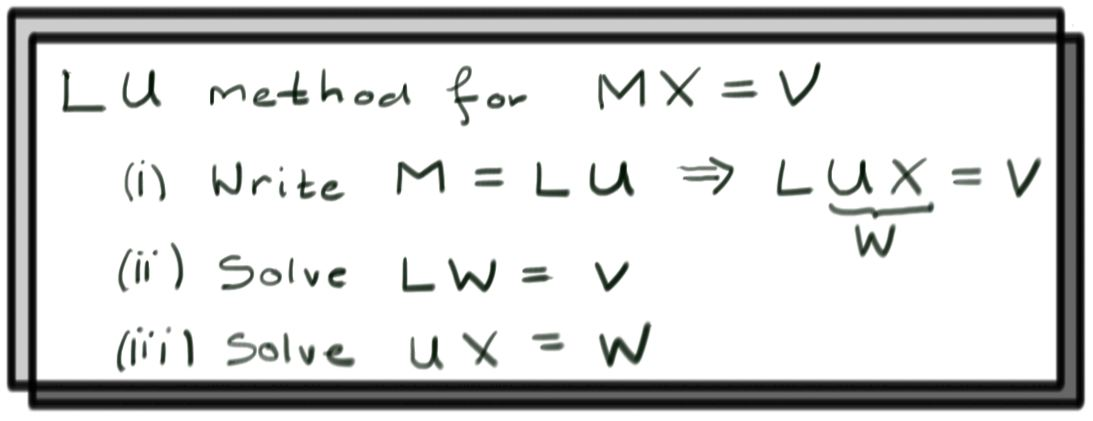
\includegraphics[scale=.3]{\luDecompPath/LU_solution.jpg}
\end{center}
%\end{figure}

\section{Finding an $LU$ Decomposition.}
\label{finding_LU_decomp}
 
For any given matrix, there are actually many different $LU$ decompositions.  However, there is a unique $LU$ decomposition in which the $L$ matrix has ones on the diagonal. In that case $L$ is called a \emph{lower unit triangular matrix}\index{Lower unit triangular matrix}.

To find the $LU$ decomposition, we'll create two sequences of matrices $L_0, L_1, \ldots$ and $U_0, U_1, \ldots$ such that at each step, $L_iU_i=M$.  Each of the $L_i$ will be lower triangular, but only the last $U_i$ will be upper triangular.

Start by setting $L_0=I$ and $U_0=M$, because $L_0U_0=M$. A main concept of this calculation is captured by the following example:

\begin{example}
Consider $$E=\begin{pmatrix}1&0\\\lambda&1\end{pmatrix}\, ,\qquad M=\begin{pmatrix}a&b&c&\cdots\\d&e&f&\cdots\end{pmatrix}\, .$$
Lets compute $EM$
$$
EM=\begin{pmatrix}a&b&c&\cdots\\d+\lambda a&e+\lambda b&f+\lambda c&\cdots\end{pmatrix}\, ,.
$$
Something neat happened here: multiplying $M$ by $E$ performed the row operation $R_2\to R_2+\lambda R-1$ on $M$.
Another interesting fact:
$$
E^{-1}:=\begin{pmatrix}1&0\\-\lambda&1\end{pmatrix}
$$ 
obeys (check this yourself...)
$$
E^{-1} E = 1\, .
$$
Hence $M=E^{-1} E M$ or, writing this out
$$
\begin{pmatrix}a&b&c&\cdots\\d&e&f&\cdots\end{pmatrix}=\begin{pmatrix}1&0\\-\lambda&1\end{pmatrix} \begin{pmatrix}a&b&c&\cdots\\d+\lambda a&e+\lambda b&f+\lambda c&\cdots\end{pmatrix}\, .
$$
Here the matrix on the left is lower triangular, while the matrix on the right has had a row operation performed on it.
\end{example}




\vspace{2mm}
We would like to  use the first row of $U_0$ to zero out the first entry of every row below it.  For our running example, $$U_0=M=\begin{pmatrix}
6 & 18 & 3 \\
2 & 12 & 1 \\
4 & 15 & 3 
\end{pmatrix}\, ,$$ so we would like to perform the row operations $R_2\to R_2 -\frac 13 R_1$ and $R_3\to R_3-\frac 23R_1$.
%so the second row minus $\frac{1}{3}$ of the first row will zero out the first entry in the second row.  Likewise, the third row minus $\frac{2}{3}$ of the first row will zero out the first entry in the third row.
If we perform these row operations on $U_0$ to produce 
$$U_1=\begin{pmatrix}
6 & 18 & 3 \\
0 & 6 & 0 \\
0 & 3 & 1 
\end{pmatrix}\, ,$$
we need to multiply this on the left by a lower triangular matrix $L_1$ so that the product $L_1U_1=M$ still.
The above example shows how to do this:
Set $L_1$ to be the lower triangular matrix whose first column is filled with the minus constants used to zero out the first column of $M$.  Then $$L_1 = \begin{pmatrix}
1 & 0 & 0 \\[1mm]
\frac{1}{3} & 1 & 0 \\[1mm]
\frac{2}{3} & 0 & 1 
\end{pmatrix}\, .$$  
%Set $U_1$ to be the matrix obtained by zeroing out the first column of $M$.  Then $U_1=\begin{pmatrix}
%6 & 18 & 3 \\
%0 & 6 & 0 \\
%0 & 3 & 1 
%\end{pmatrix}$.
By construction $L_1 U_1=M$, but you should compute this yourself as a double check.

Now repeat the process by zeroing the second column of $U_1$ below the diagonal using the second row of $U_1$ using the row operation
$R_3\to R_3-\frac 12 R_2$ to produce
$$U_2=\begin{pmatrix}6&18&3\\0&6&0\\0&0&1\end{pmatrix}\, .$$
The matrix that undoes this row operation is obtained in the same way we found $L_1$ above and is:
$$
\begin{pmatrix}
1&0&0\\
0&1&0\\
0&\frac 12& 0
\end{pmatrix}\, .
$$
Thus our answer for $L_2$ is the product of this matrix with $L_1$, namely
$$
L_2=
\begin{pmatrix}
1 & 0 & 0 \\[1mm]
\frac{1}{3} & 1 & 0 \\[1mm]
\frac{2}{3} & 0 & 1 
\end{pmatrix}\begin{pmatrix}
1&0&0\\
0&1&0\\
0&\frac 12& 0
\end{pmatrix}
=\begin{pmatrix}
1 & 0 & 0 \\[1mm]
\frac{1}{3} & 1 & 0 \\[1mm]
\frac{2}{3} & \frac{1}{2} & 1 
\end{pmatrix}\, .
$$
Notice that it is lower triangular because 

\begin{center}
\textcolor{brown}{THE PRODUCT OF LOWER TRIANGULAR MATRICES IS ALWAYS LOWER TRIANGULAR!}
\end{center}

\noindent
Moreover it is obtained by recording minus the constants used for all our row operations in the appropriate columns (this always works this way).
Moreover, $U_2$ is upper triangular and $M=L_2U_2$, we are done!
Putting this all together we have
$$M=\begin{pmatrix}
6 & 18 & 3 \\
2 & 12 & 1 \\
4 & 15 & 3 
\end{pmatrix}= \begin{pmatrix}
1 & 0 & 0 \\[1mm]
\frac{1}{3} & 1 & 0 \\[1mm]
\frac{2}{3} & \frac{1}{2} & 1 
\end{pmatrix}\begin{pmatrix}
6 & 18 & 3 \\
0 & 6 & 0 \\
0 & 0 & 1 
\end{pmatrix}\, .$$  
%Since $U_2$ is upper-triangular, we're done.  Inserting the new number into $L_1$ to get $L_2$ really is safe: the numbers in the first column don't affect the second column of $U_1$, since the first column of $U_1$ is already zeroed out.

If the matrix you're working with has more than three rows, just continue this process by zeroing out the next column below the diagonal, and repeat until there's nothing left to do.

\videoscriptlink{lu_decomposition_example.mp4}{Another $LU$ decomposition example}{scripts_lu_decomposition_example}

The fractions in the $L$ matrix are admittedly ugly.  For two matrices $LU$, we can multiply one entire column of $L$ by a constant $\lambda$ and divide the corresponding row of $U$ by the same constant without changing the product of the two matrices.  Then:

\begin{eqnarray*}
LU &=& \begin{pmatrix}
1 & 0 & 0 \\[1mm]
\frac{1}{3} & 1 & 0 \\[1mm]
\frac{2}{3} & \frac{1}{2} & 1 
\end{pmatrix}
I
\begin{pmatrix}
6 & 18 & 3 \\
0 & 6 & 0 \\
0 & 0 & 1 
\end{pmatrix} \\
&=&
\begin{pmatrix}
1 & 0 & 0 \\[1mm]
\frac{1}{3} & 1 & 0 \\[1mm]
\frac{2}{3} & \frac{1}{2} & 1 
\end{pmatrix}
\begin{pmatrix}
3 & 0 & 0 \\
0 & 6 & 0 \\
0 & 0 & 1 
\end{pmatrix}
\begin{pmatrix}
\frac{1}{3} & 0 & 0 \\[1mm]
0 & \frac{1}{6} & 0 \\[1mm]
0 & 0 & 1 
\end{pmatrix}
\begin{pmatrix}
6 & 18 & 3 \\
0 & 6 & 0 \\
0 & 0 & 1 
\end{pmatrix} \\
&=&
\begin{pmatrix}
3 & 0 & 0 \\
1 & 6 & 0 \\
2 & 3 & 1 
\end{pmatrix}\begin{pmatrix}
2 & 6 & 1 \\
0 & 1 & 0 \\
0 & 0 & 1 
\end{pmatrix}.
\end{eqnarray*}
The resulting matrix looks nicer, but isn't in standard (lower unit triangular matrix) form.

\reading{11}{2}
%\href{\webworkurl ReadingHomework11/2/}{Reading homework: problem 11.2}

For matrices that are not square, $LU$ decomposition still makes sense.  Given an $m\times n$ matrix $M$, for example we could write $M=LU$ with $L$ a square lower unit triangular matrix, and $U$ a rectangular matrix.  Then $L$ will be an $m\times m$ matrix, and $U$ will be an $m\times n$ matrix (of the same shape as $M$).  From here, the process is exactly the same as for a square matrix.  We create a sequence of matrices $L_i$ and $U_i$ that is eventually the $LU$ decomposition.  Again, we start with $L_0=I$ and $U_0=M$.

\begin{example}
Let's find the $LU$ decomposition of $M=U_0=\begin{pmatrix}
-2 & 1 & 3 \\
-4 & 4 & 1 
\end{pmatrix}$.  Since $M$ is a $2\times 3$ matrix, our decomposition will consist of a $2\times 2$ matrix and a $2\times 3$ matrix.  Then we start with $L_0=I_2=\begin{pmatrix}
1 & 0 \\
0 & 1
\end{pmatrix}$.

The next step is to zero-out the first column of $M$ below the diagonal.  There is only one row to cancel, then, and it can be removed by subtracting $2$ times the first row of $M$ to the second row of $M$.  Then:

\[
L_1=\begin{pmatrix}
1 & 0 \\
2 & 1
\end{pmatrix}, \qquad 
U_1 = \begin{pmatrix}
-2 & 1 & 3 \\
0 & 2 & -5 
\end{pmatrix}
\]
Since $U_1$ is upper triangular, we're done.  With a larger matrix, we would just continue the process.
\end{example}





\section{Block $LDU$ Decomposition}

Let $M$ be a square block matrix with square blocks $X,Y,Z,W$ such that $X^{-1}$ exists.  Then $M$ can be decomposed as a block $LDU$ decomposition, where $D$ is block diagonal, as follows:
\[
M=\begin{pmatrix}
X & Y \\
Z & W
\end{pmatrix}
\]

Then: \[M=\begin{pmatrix}
I &  0 \\
ZX^{-1} & I
\end{pmatrix}\begin{pmatrix}
X & 0 \\
0 & W-ZX^{-1}Y
\end{pmatrix}\begin{pmatrix}
I & X^{-1}Y \\
0 & I
\end{pmatrix}.\]
This can be checked explicitly simply by block-multiplying these three matrices.

\videoscriptlink{lu_decomposition_blocks.mp4}{Block $LDU$ Explanation}{scripts_lu_decomposition_blocks}

\begin{example}
For a $2\times 2$ matrix, we can regard each entry as a block.
\[
\begin{pmatrix}
1 & 2 \\
3 & 4
\end{pmatrix}=
\begin{pmatrix}
1 & 0 \\
3 & 1
\end{pmatrix}
\begin{pmatrix}
1 & 0 \\
0 & -2
\end{pmatrix}
\begin{pmatrix}
1 & 2 \\
0 & 1
\end{pmatrix}
\]
By multiplying the diagonal matrix by the upper triangular matrix, we get the standard $LU$ decomposition of the matrix.
\end{example}


%\section*{References}
%Wikipedia:
%\begin{itemize}
%\item \href{http://en.wikipedia.org/wiki/LU_decomposition}{$LU$ Decomposition}
%\item \href{http://en.wikipedia.org/wiki/Block_LU_decomposition}{Block $LU$ Decomposition}
%\end{itemize}

\section{Review Problems}



\begin{enumerate}

\item Let $D=\begin{pmatrix}
\lambda_1 & \mc0 \\
\mc0 & \lambda_2 \\
\end{pmatrix}$.
\begin{enumerate}
\item Write $D$ in terms of the vectors $e_1$ and $e_2$, and their transposes.
\item Suppose $P=\begin{pmatrix}
a & b \\
c & d \\
\end{pmatrix}$ is invertible.  Show that $D$ is similar to
\[
M=\frac{1}{ad-bc}\begin{pmatrix}
\lambda_1ad-\lambda_2bc & -(\lambda_1-\lambda_2)ab \\[1mm]
(\lambda_1-\lambda_2)cd & -\lambda_1bc + \lambda_2ad
\end{pmatrix}.
\]
\item Suppose the vectors $\rowvec{a,b}$ and $\rowvec{c,d}$ are orthogonal.  What can you say about $M$ in this case? (Hint: think about what \(M^T\) is equal to.)
\end{enumerate}

\phantomnewpage

\item \label{orthogprob} Suppose $S=\{v_1, \ldots, v_n \}$ is an \emph{orthogonal} (not orthonormal) basis for~$\Re^n$.  Then we can write any vector $v$ as $v=\sum_ic^iv_i$ for some constants $c^i$.  Find a formula for the constants $c^i$ in terms of $v$ and the vectors in~$S$.

\Videoscriptlink{orthonormal_bases_hint.mp4}{Hint}{scripts_orthonormal_bases_hint}
\phantomnewpage

\item \label{orthogprojprob} Let $u,v$ be linearly independent vectors in $\Re^3$, and $P=\spa \{ u,v\}$ be the plane spanned by $u$ and $v$.  
\begin{enumerate}
\item Is the vector $v^\bot := v-\frac{u\cdot v}{u\cdot u}u$ in the plane $P$?
\item  What is the (cosine of the) angle between $v^\bot$ and $u$?
\item %Given your solution to the above, 
How can you find a third vector perpendicular to both $u$ and $v^\bot$?
\item  Construct an orthonormal basis for $\Re^3$ from $u$ and $v$.
\item  Test your abstract formul\ae\ starting with 
\[
u=\rowvec{1 , 2 , 0} \text{ and } v=\rowvec{0 , 1 , 1}.
\]
\end{enumerate}

\Videoscriptlink{orthonormal_bases_hint3.mp4}{Hint}{scripts_orthonormal_bases_hint3}

\phantomnewpage



\item Find an orthonormal  basis for $\Re^4$ which includes $(1,1,1,1)$ using the following procedure:\\
\begin{enumerate} 
\item Pick a vector perpendicular to the vector 
$$v_1 =\colvec{1\\1\\1\\1}$$ from the solution set of the matrix equation $$v_1^Tx=0\, .$$ Pick the vector $v_2$ obtained from the standard Gaussian elimination procedure which is the coefficient of $x_2$.
\item Pick a vector perpendicular to both $v_1$ and $v_2$ from the solutions set of the matrix equation $$\colvec{v_1^T\\[1mm]v_2^T}x=0\, .$$ Pick the vector $v_3$ obtained from the standard Gaussian elimination procedure with $x_3$ as the coefficient. 
\item Pick a vector perpendicular to $v_1,v_2,$ and $v_3$ from the solution set of the matrix equation $$\colvec{v_1^T\\[1mm]v_2^T\\[1mm]v_3^T}x=0\, .$$  Pick the vector $v_4$ obtained from the standard Gaussian elimination procedure with $x_3$ as the coefficient. 
\item Normalize the four vectors obtained   above.
\end{enumerate}


\item Use the inner product $$f\cdot g := \int_0^1 f(x)g(x)dx$$  on the vector space $V={\rm span} \{1,x,x^2,x^3\}$ to perform the Gram-Schmidt procedure on the set of vectors $\{1,x,x^2,x^3\}$. 

\item Use the inner product $$f\cdot g := \int_0^{2\pi} f(x)g(x)dx$$  on the vector space $V={\rm span} \{\sin(x),\sin(2x),\sin(3x) \}$ to perform the Gram-Schmidt procedure on the set of vectors $\{\sin(x),\sin(2x),\sin(3x) \}$. \\
Try to build an orthonormal basis for the vector space $$\spa \{ \sin(nx)~| ~n\in \N \}\, .$$
%What do you suspect about the vector space $\spa \{ \sin(nx)~| ~n\in \N \}$?\\
%What do you suspect about the vector space $\spa \{ \sin(ax)~|~ a \in \Re \}$?
\item 
\begin{enumerate}
\item
Show that if $Q$ is an orthogonal $n\times n$ matrix, then $$u\dotprod v = (Qu)\dotprod (Qv)\, ,$$ for any $u,v\in \Re^n$. That is, $Q$ preserves the inner product. 
\item Does $Q$ preserve the outer product? 
\item  If the set of vectors $\{ u_1,\dots,u_n\}$ is orthonormal and $\{ \lambda_1,\cdots,\lambda_n\}$ is a set of numbers, 
then what are the eigenvalues and eigenvectors of the matrix
$M=\sum_{i=1}^n \lambda_i u_i u_i^T$? 
\item How would the eigenvectors and eigenvalues of this matrix change if we replaced  $\{ u_1,\dots,u_n\}$ by $\{ Qu_1,\dots,Q u_n\}$?
\end{enumerate}


\item Carefully write out the Gram-Schmidt procedure for the set of vectors 
$$\left\{ \colvec{1\\1\\1}, \colvec{1\\-1\\1}, \colvec{1\\1\\-1} \right\} \, .$$ Is it possible to rescale the second vector obtained in the procedure to a vector with integer components? 


\item 
\label{basisortho}
\begin{enumerate}
\item Suppose $u$ and $v$ are linearly independent.  Show that $u$ and $v^\perp$ are also linearly independent.  Explain why $\{u, v^\perp\}$ is a basis for $\spa \{u,v\}$.



\Videoscriptlink{gram_schmidt_and_orthogonal_complements_hint.mp4}{Hint}{gram_schmidt_and_orthogonal_complements_hint}

\item Repeat the previous problem, but with three independent vectors $u,v,w$
 where $v^\perp$ and $w^\perp$ are as defined by the Gram-Schmidt procedure. 
\end{enumerate}

\phantomnewpage


\item \label{QRprob} Find the $QR$ factorization of
$$
M=\begin{pmatrix}1&0&\phantom{\!-}2\\-1&2&0\\-1&-2&2
\end{pmatrix}\, .
$$

\phantomnewpage

\item Given any three vectors $u,v,w$, when do $v^\perp$ or $w^\perp$ of the Gram--Schmidt procedure vanish?

\phantomnewpage

\item For $U$ a subspace of $W$, use the subspace theorem to check that $U^\perp$ is a subspace of $W$.

\phantomnewpage


\phantomnewpage

\item %(Extra Credit) 
Let $S_n$ and $A_n$ define the space of $n \times n$ symmetric and anti-symmetric matrices, respectively. These are subspaces of the vector space $M^n_n$ of all $n\times n$ matrices. What is $\dim M^n_n$, $\dim S_n$, and $\dim A_n$? Show that $M^n_n = S_n + A_n$. Define an inner product on square matrices
$$
M\cdot N ={\rm tr} MN\, .
$$
Is $A_n^{\perp}=S_n$? Is $M^n_n = S_n \oplus A_n$?

%\emph{Hint: Note that $\dim S_n = \dim U_n$ where $U_n$ is the vector space of all $n \times n$ upper triangular matrices, and also note that $\dim A_n = \dim \widetilde{U}_n$ where $\widetilde{U}_n$ is the vector space of all strictly $n \times n$ upper triangular matrices (\emph{i.e.} the diagonal entries are all 0).}

\item The vector space $V={\rm span} \{ \sin(t),\sin(2t), \sin(3t) , \sin(3t)\}$ has an inner product: 
$$f\cdot g:=\int _0^{2\pi}f(t)g(t) dt\, .$$ Find the orthogonal compliment to $U={\rm span} \{ \sin(t)+\sin(2t) \}$ in $V$. Express $\sin(t)-\sin(2t)$ as  the sum of vectors from $U$ and $U^\perp$.

\end{enumerate}

\phantomnewpage

\newpage


\chapter{\luDecompTitle}
\label{LUdecomp}

Certain matrices are easier to work with than others.  In this section, we will see how to write any square\footnote{The case where $M$ is not square is dealt with at the end of the lecture.} matrix $M$ as the product of two simpler matrices.  We will write $$M=LU\, ,$$ where:
\begin{itemize}
\item $L$ is \emph{lower triangular}\index{Lower triangular matrix}.  This means that all entries above the main diagonal are zero.  In notation,
$L=(l^i_j)$ with $l^i_j=0$ for all $j>i$.
\[L=\begin{pmatrix}
l^1_1 & 0 & 0 & \cdots \\
l^2_1 & l^2_2 & 0 & \cdots \\
l^3_1 & l^3_2 & l^3_3 & \cdots \\
\vdots & \vdots & \vdots & \ddots \\
\end{pmatrix}
\]

\item $U$ is \emph{upper triangular}\index{Upper triangular matrix}.  This means that all entries below the main diagonal are zero.  In notation,
$U=(u^i_j)$ with $u^i_j=0$ for all $j<i$.
\[U=\begin{pmatrix}
u^1_1 & u^1_2 & u^1_3 & \cdots \\
0 & u^2_2 & u^2_3 & \cdots \\
0 & 0 & u^3_3 & \cdots \\
\vdots & \vdots & \vdots & \ddots \\
\end{pmatrix}
\]
\end{itemize}
$M=LU$ is called an \emph{$LU$ decomposition}\index{LU@$LU$ decomposition} of $M$.

This is a useful trick for  computational reasons; it is much easier to compute the inverse of an upper or lower triangular matrix than general matrices.  Since inverses are useful for solving linear systems, this makes solving any linear system associated to the matrix much faster as well.  The determinant---a very important quantity associated with any square matrix---is very easy to compute for triangular matrices.

\begin{example}
Linear systems associated to upper triangular matrices are very easy to solve by back substitution.
\[
\begin{amatrix}{2}
a & b & 1 \\
0 & c & e \\
\end{amatrix} \ \Rightarrow \ y=\frac{e}{c}\, , \quad x=\frac{1}{a}\left(1-\frac{be}{c}\right)
\]

\[
\begin{amatrix}{3}
1 & 0 & 0 & d \\
a & 1 & 0 & e \\
b & c & 1 & f \\
\end{amatrix} \Rightarrow x=d\, , \qquad y=e-ad\, , \qquad z=f-bd-c(e-ad)
\]
For lower triangular matrices, \emph{back} substitution\index{Back substitution} gives a quick solution; for upper triangular matrices, \emph{forward} substitution\index{Forward substitution} gives the solution.
\end{example}





\section{Using $LU$ Decomposition to Solve Linear Systems}

Suppose we have $M=LU$ and want to solve the system
\[
MX=LUX=V.
\]

\begin{itemize}
\item{Step 1:} Set $W=\colvec{u\\v\\w}=UX$.  

\item{Step 2:} Solve the system $LW=V$.  This should be simple by forward substitution since $L$ is lower triangular.  Suppose the solution to $LW=V$ is $W_0$.  

\item{Step 3:} Now solve the system $UX=W_0$.  This should be easy by backward substitution, since $U$ is upper triangular.  The solution to this system is the solution to the original system.
\end{itemize}
We can think of this as using the matrix $L$ to perform row operations on the matrix $U$ in order to solve the system; this idea also appears in the  study of determinants.

%\href{\webworkurl ReadingHomework11/1/}{Reading homework: problem 11.1}
\reading{11}{1}

\begin{example}
Consider the linear system:
\[
      \begin{linsys}{4}
            6x & +&18y & +&3z         &=& 3  \\[1mm]
            2x & +&12y & +&z	    &=& 19 \\[1mm]
            4x & +&15y & +&3z         &=& 0  
      \end{linsys}
\]

An $LU$ decomposition for the associated matrix $M$ is:
\[
\begin{pmatrix}
6 & 18 & 3 \\
2 & 12 & 1 \\
4 & 15 & 3 
\end{pmatrix} =
\begin{pmatrix}
3 & 0 & 0 \\
1 & 6 & 0 \\
2 & 3 & 1 
\end{pmatrix}
\begin{pmatrix}
2 & 6 & 1 \\
0 & 1 & 0 \\
0 & 0 & 1 
\end{pmatrix}.
\]

\begin{itemize}
\item{Step 1:} \hypertarget{LUproc}{Set} $W=\colvec{u\\v\\w}=UX$.  

\item{Step 2:} Solve the system $LW=V$:

\[
\begin{pmatrix}
3 & 0 & 0 \\
1 & 6 & 0 \\
2 & 3 & 1 
\end{pmatrix}
\colvec{u\\v\\w} =
\colvec{3\\19\\0}
\]

By substitution, we get $u=1$, $v=3$, and $w=-11$.  Then 
\[W_0=\colvec{1\\3\\-11}\]

\item{Step 3:} Solve the system $UX=W_0$.  
\[
\begin{pmatrix}
2 & 6 & 1 \\
0 & 1 & 0 \\
0 & 0 & 1 
\end{pmatrix}
\colvec{x\\y\\z} =
\colvec{1\\3\\-11}
\]
Back substitution gives $z=-11, y=3$, and $x=-3$.  

Then $X=\colvec{-3\\3\\-11}$, and we're done.
\end{itemize}
\end{example}

\videoscriptlink{lu_decomposition_using_lu_decomp.mp4}{Using a $LU$ decomposition}{scripts_lu_decomposition_using_lu_example}

%\begin{figure}
\begin{center}
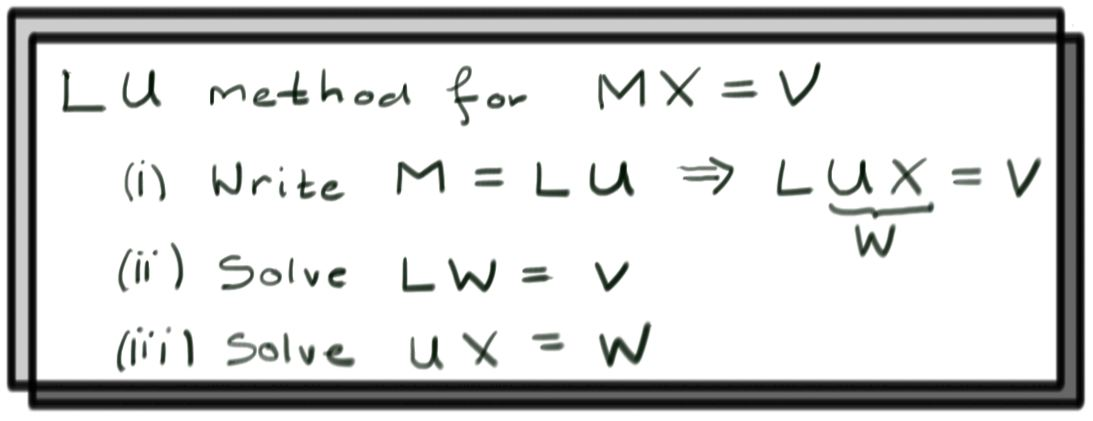
\includegraphics[scale=.3]{\luDecompPath/LU_solution.jpg}
\end{center}
%\end{figure}

\section{Finding an $LU$ Decomposition.}
\label{finding_LU_decomp}
 
For any given matrix, there are actually many different $LU$ decompositions.  However, there is a unique $LU$ decomposition in which the $L$ matrix has ones on the diagonal. In that case $L$ is called a \emph{lower unit triangular matrix}\index{Lower unit triangular matrix}.

To find the $LU$ decomposition, we'll create two sequences of matrices $L_0, L_1, \ldots$ and $U_0, U_1, \ldots$ such that at each step, $L_iU_i=M$.  Each of the $L_i$ will be lower triangular, but only the last $U_i$ will be upper triangular.

Start by setting $L_0=I$ and $U_0=M$, because $L_0U_0=M$. A main concept of this calculation is captured by the following example:

\begin{example}
Consider $$E=\begin{pmatrix}1&0\\\lambda&1\end{pmatrix}\, ,\qquad M=\begin{pmatrix}a&b&c&\cdots\\d&e&f&\cdots\end{pmatrix}\, .$$
Lets compute $EM$
$$
EM=\begin{pmatrix}a&b&c&\cdots\\d+\lambda a&e+\lambda b&f+\lambda c&\cdots\end{pmatrix}\, ,.
$$
Something neat happened here: multiplying $M$ by $E$ performed the row operation $R_2\to R_2+\lambda R-1$ on $M$.
Another interesting fact:
$$
E^{-1}:=\begin{pmatrix}1&0\\-\lambda&1\end{pmatrix}
$$ 
obeys (check this yourself...)
$$
E^{-1} E = 1\, .
$$
Hence $M=E^{-1} E M$ or, writing this out
$$
\begin{pmatrix}a&b&c&\cdots\\d&e&f&\cdots\end{pmatrix}=\begin{pmatrix}1&0\\-\lambda&1\end{pmatrix} \begin{pmatrix}a&b&c&\cdots\\d+\lambda a&e+\lambda b&f+\lambda c&\cdots\end{pmatrix}\, .
$$
Here the matrix on the left is lower triangular, while the matrix on the right has had a row operation performed on it.
\end{example}




\vspace{2mm}
We would like to  use the first row of $U_0$ to zero out the first entry of every row below it.  For our running example, $$U_0=M=\begin{pmatrix}
6 & 18 & 3 \\
2 & 12 & 1 \\
4 & 15 & 3 
\end{pmatrix}\, ,$$ so we would like to perform the row operations $R_2\to R_2 -\frac 13 R_1$ and $R_3\to R_3-\frac 23R_1$.
%so the second row minus $\frac{1}{3}$ of the first row will zero out the first entry in the second row.  Likewise, the third row minus $\frac{2}{3}$ of the first row will zero out the first entry in the third row.
If we perform these row operations on $U_0$ to produce 
$$U_1=\begin{pmatrix}
6 & 18 & 3 \\
0 & 6 & 0 \\
0 & 3 & 1 
\end{pmatrix}\, ,$$
we need to multiply this on the left by a lower triangular matrix $L_1$ so that the product $L_1U_1=M$ still.
The above example shows how to do this:
Set $L_1$ to be the lower triangular matrix whose first column is filled with the minus constants used to zero out the first column of $M$.  Then $$L_1 = \begin{pmatrix}
1 & 0 & 0 \\[1mm]
\frac{1}{3} & 1 & 0 \\[1mm]
\frac{2}{3} & 0 & 1 
\end{pmatrix}\, .$$  
%Set $U_1$ to be the matrix obtained by zeroing out the first column of $M$.  Then $U_1=\begin{pmatrix}
%6 & 18 & 3 \\
%0 & 6 & 0 \\
%0 & 3 & 1 
%\end{pmatrix}$.
By construction $L_1 U_1=M$, but you should compute this yourself as a double check.

Now repeat the process by zeroing the second column of $U_1$ below the diagonal using the second row of $U_1$ using the row operation
$R_3\to R_3-\frac 12 R_2$ to produce
$$U_2=\begin{pmatrix}6&18&3\\0&6&0\\0&0&1\end{pmatrix}\, .$$
The matrix that undoes this row operation is obtained in the same way we found $L_1$ above and is:
$$
\begin{pmatrix}
1&0&0\\
0&1&0\\
0&\frac 12& 0
\end{pmatrix}\, .
$$
Thus our answer for $L_2$ is the product of this matrix with $L_1$, namely
$$
L_2=
\begin{pmatrix}
1 & 0 & 0 \\[1mm]
\frac{1}{3} & 1 & 0 \\[1mm]
\frac{2}{3} & 0 & 1 
\end{pmatrix}\begin{pmatrix}
1&0&0\\
0&1&0\\
0&\frac 12& 0
\end{pmatrix}
=\begin{pmatrix}
1 & 0 & 0 \\[1mm]
\frac{1}{3} & 1 & 0 \\[1mm]
\frac{2}{3} & \frac{1}{2} & 1 
\end{pmatrix}\, .
$$
Notice that it is lower triangular because 

\begin{center}
\textcolor{brown}{THE PRODUCT OF LOWER TRIANGULAR MATRICES IS ALWAYS LOWER TRIANGULAR!}
\end{center}

\noindent
Moreover it is obtained by recording minus the constants used for all our row operations in the appropriate columns (this always works this way).
Moreover, $U_2$ is upper triangular and $M=L_2U_2$, we are done!
Putting this all together we have
$$M=\begin{pmatrix}
6 & 18 & 3 \\
2 & 12 & 1 \\
4 & 15 & 3 
\end{pmatrix}= \begin{pmatrix}
1 & 0 & 0 \\[1mm]
\frac{1}{3} & 1 & 0 \\[1mm]
\frac{2}{3} & \frac{1}{2} & 1 
\end{pmatrix}\begin{pmatrix}
6 & 18 & 3 \\
0 & 6 & 0 \\
0 & 0 & 1 
\end{pmatrix}\, .$$  
%Since $U_2$ is upper-triangular, we're done.  Inserting the new number into $L_1$ to get $L_2$ really is safe: the numbers in the first column don't affect the second column of $U_1$, since the first column of $U_1$ is already zeroed out.

If the matrix you're working with has more than three rows, just continue this process by zeroing out the next column below the diagonal, and repeat until there's nothing left to do.

\videoscriptlink{lu_decomposition_example.mp4}{Another $LU$ decomposition example}{scripts_lu_decomposition_example}

The fractions in the $L$ matrix are admittedly ugly.  For two matrices $LU$, we can multiply one entire column of $L$ by a constant $\lambda$ and divide the corresponding row of $U$ by the same constant without changing the product of the two matrices.  Then:

\begin{eqnarray*}
LU &=& \begin{pmatrix}
1 & 0 & 0 \\[1mm]
\frac{1}{3} & 1 & 0 \\[1mm]
\frac{2}{3} & \frac{1}{2} & 1 
\end{pmatrix}
I
\begin{pmatrix}
6 & 18 & 3 \\
0 & 6 & 0 \\
0 & 0 & 1 
\end{pmatrix} \\
&=&
\begin{pmatrix}
1 & 0 & 0 \\[1mm]
\frac{1}{3} & 1 & 0 \\[1mm]
\frac{2}{3} & \frac{1}{2} & 1 
\end{pmatrix}
\begin{pmatrix}
3 & 0 & 0 \\
0 & 6 & 0 \\
0 & 0 & 1 
\end{pmatrix}
\begin{pmatrix}
\frac{1}{3} & 0 & 0 \\[1mm]
0 & \frac{1}{6} & 0 \\[1mm]
0 & 0 & 1 
\end{pmatrix}
\begin{pmatrix}
6 & 18 & 3 \\
0 & 6 & 0 \\
0 & 0 & 1 
\end{pmatrix} \\
&=&
\begin{pmatrix}
3 & 0 & 0 \\
1 & 6 & 0 \\
2 & 3 & 1 
\end{pmatrix}\begin{pmatrix}
2 & 6 & 1 \\
0 & 1 & 0 \\
0 & 0 & 1 
\end{pmatrix}.
\end{eqnarray*}
The resulting matrix looks nicer, but isn't in standard (lower unit triangular matrix) form.

\reading{11}{2}
%\href{\webworkurl ReadingHomework11/2/}{Reading homework: problem 11.2}

For matrices that are not square, $LU$ decomposition still makes sense.  Given an $m\times n$ matrix $M$, for example we could write $M=LU$ with $L$ a square lower unit triangular matrix, and $U$ a rectangular matrix.  Then $L$ will be an $m\times m$ matrix, and $U$ will be an $m\times n$ matrix (of the same shape as $M$).  From here, the process is exactly the same as for a square matrix.  We create a sequence of matrices $L_i$ and $U_i$ that is eventually the $LU$ decomposition.  Again, we start with $L_0=I$ and $U_0=M$.

\begin{example}
Let's find the $LU$ decomposition of $M=U_0=\begin{pmatrix}
-2 & 1 & 3 \\
-4 & 4 & 1 
\end{pmatrix}$.  Since $M$ is a $2\times 3$ matrix, our decomposition will consist of a $2\times 2$ matrix and a $2\times 3$ matrix.  Then we start with $L_0=I_2=\begin{pmatrix}
1 & 0 \\
0 & 1
\end{pmatrix}$.

The next step is to zero-out the first column of $M$ below the diagonal.  There is only one row to cancel, then, and it can be removed by subtracting $2$ times the first row of $M$ to the second row of $M$.  Then:

\[
L_1=\begin{pmatrix}
1 & 0 \\
2 & 1
\end{pmatrix}, \qquad 
U_1 = \begin{pmatrix}
-2 & 1 & 3 \\
0 & 2 & -5 
\end{pmatrix}
\]
Since $U_1$ is upper triangular, we're done.  With a larger matrix, we would just continue the process.
\end{example}





\section{Block $LDU$ Decomposition}

Let $M$ be a square block matrix with square blocks $X,Y,Z,W$ such that $X^{-1}$ exists.  Then $M$ can be decomposed as a block $LDU$ decomposition, where $D$ is block diagonal, as follows:
\[
M=\begin{pmatrix}
X & Y \\
Z & W
\end{pmatrix}
\]

Then: \[M=\begin{pmatrix}
I &  0 \\
ZX^{-1} & I
\end{pmatrix}\begin{pmatrix}
X & 0 \\
0 & W-ZX^{-1}Y
\end{pmatrix}\begin{pmatrix}
I & X^{-1}Y \\
0 & I
\end{pmatrix}.\]
This can be checked explicitly simply by block-multiplying these three matrices.

\videoscriptlink{lu_decomposition_blocks.mp4}{Block $LDU$ Explanation}{scripts_lu_decomposition_blocks}

\begin{example}
For a $2\times 2$ matrix, we can regard each entry as a block.
\[
\begin{pmatrix}
1 & 2 \\
3 & 4
\end{pmatrix}=
\begin{pmatrix}
1 & 0 \\
3 & 1
\end{pmatrix}
\begin{pmatrix}
1 & 0 \\
0 & -2
\end{pmatrix}
\begin{pmatrix}
1 & 2 \\
0 & 1
\end{pmatrix}
\]
By multiplying the diagonal matrix by the upper triangular matrix, we get the standard $LU$ decomposition of the matrix.
\end{example}


%\section*{References}
%Wikipedia:
%\begin{itemize}
%\item \href{http://en.wikipedia.org/wiki/LU_decomposition}{$LU$ Decomposition}
%\item \href{http://en.wikipedia.org/wiki/Block_LU_decomposition}{Block $LU$ Decomposition}
%\end{itemize}

\section{Review Problems}



\begin{enumerate}

\item Let $D=\begin{pmatrix}
\lambda_1 & \mc0 \\
\mc0 & \lambda_2 \\
\end{pmatrix}$.
\begin{enumerate}
\item Write $D$ in terms of the vectors $e_1$ and $e_2$, and their transposes.
\item Suppose $P=\begin{pmatrix}
a & b \\
c & d \\
\end{pmatrix}$ is invertible.  Show that $D$ is similar to
\[
M=\frac{1}{ad-bc}\begin{pmatrix}
\lambda_1ad-\lambda_2bc & -(\lambda_1-\lambda_2)ab \\[1mm]
(\lambda_1-\lambda_2)cd & -\lambda_1bc + \lambda_2ad
\end{pmatrix}.
\]
\item Suppose the vectors $\rowvec{a,b}$ and $\rowvec{c,d}$ are orthogonal.  What can you say about $M$ in this case? (Hint: think about what \(M^T\) is equal to.)
\end{enumerate}

\phantomnewpage

\item \label{orthogprob} Suppose $S=\{v_1, \ldots, v_n \}$ is an \emph{orthogonal} (not orthonormal) basis for~$\Re^n$.  Then we can write any vector $v$ as $v=\sum_ic^iv_i$ for some constants $c^i$.  Find a formula for the constants $c^i$ in terms of $v$ and the vectors in~$S$.

\Videoscriptlink{orthonormal_bases_hint.mp4}{Hint}{scripts_orthonormal_bases_hint}
\phantomnewpage

\item \label{orthogprojprob} Let $u,v$ be linearly independent vectors in $\Re^3$, and $P=\spa \{ u,v\}$ be the plane spanned by $u$ and $v$.  
\begin{enumerate}
\item Is the vector $v^\bot := v-\frac{u\cdot v}{u\cdot u}u$ in the plane $P$?
\item  What is the (cosine of the) angle between $v^\bot$ and $u$?
\item %Given your solution to the above, 
How can you find a third vector perpendicular to both $u$ and $v^\bot$?
\item  Construct an orthonormal basis for $\Re^3$ from $u$ and $v$.
\item  Test your abstract formul\ae\ starting with 
\[
u=\rowvec{1 , 2 , 0} \text{ and } v=\rowvec{0 , 1 , 1}.
\]
\end{enumerate}

\Videoscriptlink{orthonormal_bases_hint3.mp4}{Hint}{scripts_orthonormal_bases_hint3}

\phantomnewpage



\item Find an orthonormal  basis for $\Re^4$ which includes $(1,1,1,1)$ using the following procedure:\\
\begin{enumerate} 
\item Pick a vector perpendicular to the vector 
$$v_1 =\colvec{1\\1\\1\\1}$$ from the solution set of the matrix equation $$v_1^Tx=0\, .$$ Pick the vector $v_2$ obtained from the standard Gaussian elimination procedure which is the coefficient of $x_2$.
\item Pick a vector perpendicular to both $v_1$ and $v_2$ from the solutions set of the matrix equation $$\colvec{v_1^T\\[1mm]v_2^T}x=0\, .$$ Pick the vector $v_3$ obtained from the standard Gaussian elimination procedure with $x_3$ as the coefficient. 
\item Pick a vector perpendicular to $v_1,v_2,$ and $v_3$ from the solution set of the matrix equation $$\colvec{v_1^T\\[1mm]v_2^T\\[1mm]v_3^T}x=0\, .$$  Pick the vector $v_4$ obtained from the standard Gaussian elimination procedure with $x_3$ as the coefficient. 
\item Normalize the four vectors obtained   above.
\end{enumerate}


\item Use the inner product $$f\cdot g := \int_0^1 f(x)g(x)dx$$  on the vector space $V={\rm span} \{1,x,x^2,x^3\}$ to perform the Gram-Schmidt procedure on the set of vectors $\{1,x,x^2,x^3\}$. 

\item Use the inner product $$f\cdot g := \int_0^{2\pi} f(x)g(x)dx$$  on the vector space $V={\rm span} \{\sin(x),\sin(2x),\sin(3x) \}$ to perform the Gram-Schmidt procedure on the set of vectors $\{\sin(x),\sin(2x),\sin(3x) \}$. \\
Try to build an orthonormal basis for the vector space $$\spa \{ \sin(nx)~| ~n\in \N \}\, .$$
%What do you suspect about the vector space $\spa \{ \sin(nx)~| ~n\in \N \}$?\\
%What do you suspect about the vector space $\spa \{ \sin(ax)~|~ a \in \Re \}$?
\item 
\begin{enumerate}
\item
Show that if $Q$ is an orthogonal $n\times n$ matrix, then $$u\dotprod v = (Qu)\dotprod (Qv)\, ,$$ for any $u,v\in \Re^n$. That is, $Q$ preserves the inner product. 
\item Does $Q$ preserve the outer product? 
\item  If the set of vectors $\{ u_1,\dots,u_n\}$ is orthonormal and $\{ \lambda_1,\cdots,\lambda_n\}$ is a set of numbers, 
then what are the eigenvalues and eigenvectors of the matrix
$M=\sum_{i=1}^n \lambda_i u_i u_i^T$? 
\item How would the eigenvectors and eigenvalues of this matrix change if we replaced  $\{ u_1,\dots,u_n\}$ by $\{ Qu_1,\dots,Q u_n\}$?
\end{enumerate}


\item Carefully write out the Gram-Schmidt procedure for the set of vectors 
$$\left\{ \colvec{1\\1\\1}, \colvec{1\\-1\\1}, \colvec{1\\1\\-1} \right\} \, .$$ Is it possible to rescale the second vector obtained in the procedure to a vector with integer components? 


\item 
\label{basisortho}
\begin{enumerate}
\item Suppose $u$ and $v$ are linearly independent.  Show that $u$ and $v^\perp$ are also linearly independent.  Explain why $\{u, v^\perp\}$ is a basis for $\spa \{u,v\}$.



\Videoscriptlink{gram_schmidt_and_orthogonal_complements_hint.mp4}{Hint}{gram_schmidt_and_orthogonal_complements_hint}

\item Repeat the previous problem, but with three independent vectors $u,v,w$
 where $v^\perp$ and $w^\perp$ are as defined by the Gram-Schmidt procedure. 
\end{enumerate}

\phantomnewpage


\item \label{QRprob} Find the $QR$ factorization of
$$
M=\begin{pmatrix}1&0&\phantom{\!-}2\\-1&2&0\\-1&-2&2
\end{pmatrix}\, .
$$

\phantomnewpage

\item Given any three vectors $u,v,w$, when do $v^\perp$ or $w^\perp$ of the Gram--Schmidt procedure vanish?

\phantomnewpage

\item For $U$ a subspace of $W$, use the subspace theorem to check that $U^\perp$ is a subspace of $W$.

\phantomnewpage


\phantomnewpage

\item %(Extra Credit) 
Let $S_n$ and $A_n$ define the space of $n \times n$ symmetric and anti-symmetric matrices, respectively. These are subspaces of the vector space $M^n_n$ of all $n\times n$ matrices. What is $\dim M^n_n$, $\dim S_n$, and $\dim A_n$? Show that $M^n_n = S_n + A_n$. Define an inner product on square matrices
$$
M\cdot N ={\rm tr} MN\, .
$$
Is $A_n^{\perp}=S_n$? Is $M^n_n = S_n \oplus A_n$?

%\emph{Hint: Note that $\dim S_n = \dim U_n$ where $U_n$ is the vector space of all $n \times n$ upper triangular matrices, and also note that $\dim A_n = \dim \widetilde{U}_n$ where $\widetilde{U}_n$ is the vector space of all strictly $n \times n$ upper triangular matrices (\emph{i.e.} the diagonal entries are all 0).}

\item The vector space $V={\rm span} \{ \sin(t),\sin(2t), \sin(3t) , \sin(3t)\}$ has an inner product: 
$$f\cdot g:=\int _0^{2\pi}f(t)g(t) dt\, .$$ Find the orthogonal compliment to $U={\rm span} \{ \sin(t)+\sin(2t) \}$ in $V$. Express $\sin(t)-\sin(2t)$ as  the sum of vectors from $U$ and $U^\perp$.

\end{enumerate}

\phantomnewpage

\newpage


\chapter{\luDecompTitle}
\label{LUdecomp}

Certain matrices are easier to work with than others.  In this section, we will see how to write any square\footnote{The case where $M$ is not square is dealt with at the end of the lecture.} matrix $M$ as the product of two simpler matrices.  We will write $$M=LU\, ,$$ where:
\begin{itemize}
\item $L$ is \emph{lower triangular}\index{Lower triangular matrix}.  This means that all entries above the main diagonal are zero.  In notation,
$L=(l^i_j)$ with $l^i_j=0$ for all $j>i$.
\[L=\begin{pmatrix}
l^1_1 & 0 & 0 & \cdots \\
l^2_1 & l^2_2 & 0 & \cdots \\
l^3_1 & l^3_2 & l^3_3 & \cdots \\
\vdots & \vdots & \vdots & \ddots \\
\end{pmatrix}
\]

\item $U$ is \emph{upper triangular}\index{Upper triangular matrix}.  This means that all entries below the main diagonal are zero.  In notation,
$U=(u^i_j)$ with $u^i_j=0$ for all $j<i$.
\[U=\begin{pmatrix}
u^1_1 & u^1_2 & u^1_3 & \cdots \\
0 & u^2_2 & u^2_3 & \cdots \\
0 & 0 & u^3_3 & \cdots \\
\vdots & \vdots & \vdots & \ddots \\
\end{pmatrix}
\]
\end{itemize}
$M=LU$ is called an \emph{$LU$ decomposition}\index{LU@$LU$ decomposition} of $M$.

This is a useful trick for  computational reasons; it is much easier to compute the inverse of an upper or lower triangular matrix than general matrices.  Since inverses are useful for solving linear systems, this makes solving any linear system associated to the matrix much faster as well.  The determinant---a very important quantity associated with any square matrix---is very easy to compute for triangular matrices.

\begin{example}
Linear systems associated to upper triangular matrices are very easy to solve by back substitution.
\[
\begin{amatrix}{2}
a & b & 1 \\
0 & c & e \\
\end{amatrix} \ \Rightarrow \ y=\frac{e}{c}\, , \quad x=\frac{1}{a}\left(1-\frac{be}{c}\right)
\]

\[
\begin{amatrix}{3}
1 & 0 & 0 & d \\
a & 1 & 0 & e \\
b & c & 1 & f \\
\end{amatrix} \Rightarrow x=d\, , \qquad y=e-ad\, , \qquad z=f-bd-c(e-ad)
\]
For lower triangular matrices, \emph{back} substitution\index{Back substitution} gives a quick solution; for upper triangular matrices, \emph{forward} substitution\index{Forward substitution} gives the solution.
\end{example}





\section{Using $LU$ Decomposition to Solve Linear Systems}

Suppose we have $M=LU$ and want to solve the system
\[
MX=LUX=V.
\]

\begin{itemize}
\item{Step 1:} Set $W=\colvec{u\\v\\w}=UX$.  

\item{Step 2:} Solve the system $LW=V$.  This should be simple by forward substitution since $L$ is lower triangular.  Suppose the solution to $LW=V$ is $W_0$.  

\item{Step 3:} Now solve the system $UX=W_0$.  This should be easy by backward substitution, since $U$ is upper triangular.  The solution to this system is the solution to the original system.
\end{itemize}
We can think of this as using the matrix $L$ to perform row operations on the matrix $U$ in order to solve the system; this idea also appears in the  study of determinants.

%\href{\webworkurl ReadingHomework11/1/}{Reading homework: problem 11.1}
\reading{11}{1}

\begin{example}
Consider the linear system:
\[
      \begin{linsys}{4}
            6x & +&18y & +&3z         &=& 3  \\[1mm]
            2x & +&12y & +&z	    &=& 19 \\[1mm]
            4x & +&15y & +&3z         &=& 0  
      \end{linsys}
\]

An $LU$ decomposition for the associated matrix $M$ is:
\[
\begin{pmatrix}
6 & 18 & 3 \\
2 & 12 & 1 \\
4 & 15 & 3 
\end{pmatrix} =
\begin{pmatrix}
3 & 0 & 0 \\
1 & 6 & 0 \\
2 & 3 & 1 
\end{pmatrix}
\begin{pmatrix}
2 & 6 & 1 \\
0 & 1 & 0 \\
0 & 0 & 1 
\end{pmatrix}.
\]

\begin{itemize}
\item{Step 1:} \hypertarget{LUproc}{Set} $W=\colvec{u\\v\\w}=UX$.  

\item{Step 2:} Solve the system $LW=V$:

\[
\begin{pmatrix}
3 & 0 & 0 \\
1 & 6 & 0 \\
2 & 3 & 1 
\end{pmatrix}
\colvec{u\\v\\w} =
\colvec{3\\19\\0}
\]

By substitution, we get $u=1$, $v=3$, and $w=-11$.  Then 
\[W_0=\colvec{1\\3\\-11}\]

\item{Step 3:} Solve the system $UX=W_0$.  
\[
\begin{pmatrix}
2 & 6 & 1 \\
0 & 1 & 0 \\
0 & 0 & 1 
\end{pmatrix}
\colvec{x\\y\\z} =
\colvec{1\\3\\-11}
\]
Back substitution gives $z=-11, y=3$, and $x=-3$.  

Then $X=\colvec{-3\\3\\-11}$, and we're done.
\end{itemize}
\end{example}

\videoscriptlink{lu_decomposition_using_lu_decomp.mp4}{Using a $LU$ decomposition}{scripts_lu_decomposition_using_lu_example}

%\begin{figure}
\begin{center}
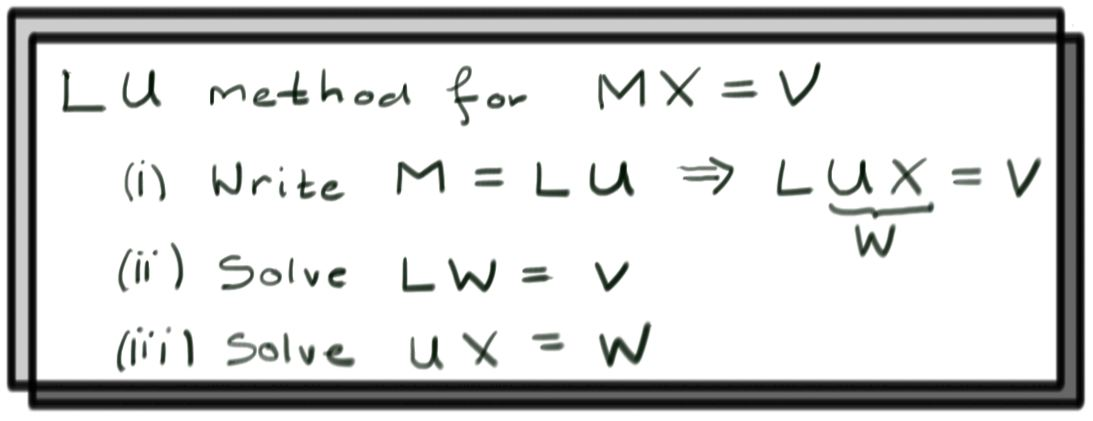
\includegraphics[scale=.3]{\luDecompPath/LU_solution.jpg}
\end{center}
%\end{figure}

\section{Finding an $LU$ Decomposition.}
\label{finding_LU_decomp}
 
For any given matrix, there are actually many different $LU$ decompositions.  However, there is a unique $LU$ decomposition in which the $L$ matrix has ones on the diagonal. In that case $L$ is called a \emph{lower unit triangular matrix}\index{Lower unit triangular matrix}.

To find the $LU$ decomposition, we'll create two sequences of matrices $L_0, L_1, \ldots$ and $U_0, U_1, \ldots$ such that at each step, $L_iU_i=M$.  Each of the $L_i$ will be lower triangular, but only the last $U_i$ will be upper triangular.

Start by setting $L_0=I$ and $U_0=M$, because $L_0U_0=M$. A main concept of this calculation is captured by the following example:

\begin{example}
Consider $$E=\begin{pmatrix}1&0\\\lambda&1\end{pmatrix}\, ,\qquad M=\begin{pmatrix}a&b&c&\cdots\\d&e&f&\cdots\end{pmatrix}\, .$$
Lets compute $EM$
$$
EM=\begin{pmatrix}a&b&c&\cdots\\d+\lambda a&e+\lambda b&f+\lambda c&\cdots\end{pmatrix}\, ,.
$$
Something neat happened here: multiplying $M$ by $E$ performed the row operation $R_2\to R_2+\lambda R-1$ on $M$.
Another interesting fact:
$$
E^{-1}:=\begin{pmatrix}1&0\\-\lambda&1\end{pmatrix}
$$ 
obeys (check this yourself...)
$$
E^{-1} E = 1\, .
$$
Hence $M=E^{-1} E M$ or, writing this out
$$
\begin{pmatrix}a&b&c&\cdots\\d&e&f&\cdots\end{pmatrix}=\begin{pmatrix}1&0\\-\lambda&1\end{pmatrix} \begin{pmatrix}a&b&c&\cdots\\d+\lambda a&e+\lambda b&f+\lambda c&\cdots\end{pmatrix}\, .
$$
Here the matrix on the left is lower triangular, while the matrix on the right has had a row operation performed on it.
\end{example}




\vspace{2mm}
We would like to  use the first row of $U_0$ to zero out the first entry of every row below it.  For our running example, $$U_0=M=\begin{pmatrix}
6 & 18 & 3 \\
2 & 12 & 1 \\
4 & 15 & 3 
\end{pmatrix}\, ,$$ so we would like to perform the row operations $R_2\to R_2 -\frac 13 R_1$ and $R_3\to R_3-\frac 23R_1$.
%so the second row minus $\frac{1}{3}$ of the first row will zero out the first entry in the second row.  Likewise, the third row minus $\frac{2}{3}$ of the first row will zero out the first entry in the third row.
If we perform these row operations on $U_0$ to produce 
$$U_1=\begin{pmatrix}
6 & 18 & 3 \\
0 & 6 & 0 \\
0 & 3 & 1 
\end{pmatrix}\, ,$$
we need to multiply this on the left by a lower triangular matrix $L_1$ so that the product $L_1U_1=M$ still.
The above example shows how to do this:
Set $L_1$ to be the lower triangular matrix whose first column is filled with the minus constants used to zero out the first column of $M$.  Then $$L_1 = \begin{pmatrix}
1 & 0 & 0 \\[1mm]
\frac{1}{3} & 1 & 0 \\[1mm]
\frac{2}{3} & 0 & 1 
\end{pmatrix}\, .$$  
%Set $U_1$ to be the matrix obtained by zeroing out the first column of $M$.  Then $U_1=\begin{pmatrix}
%6 & 18 & 3 \\
%0 & 6 & 0 \\
%0 & 3 & 1 
%\end{pmatrix}$.
By construction $L_1 U_1=M$, but you should compute this yourself as a double check.

Now repeat the process by zeroing the second column of $U_1$ below the diagonal using the second row of $U_1$ using the row operation
$R_3\to R_3-\frac 12 R_2$ to produce
$$U_2=\begin{pmatrix}6&18&3\\0&6&0\\0&0&1\end{pmatrix}\, .$$
The matrix that undoes this row operation is obtained in the same way we found $L_1$ above and is:
$$
\begin{pmatrix}
1&0&0\\
0&1&0\\
0&\frac 12& 0
\end{pmatrix}\, .
$$
Thus our answer for $L_2$ is the product of this matrix with $L_1$, namely
$$
L_2=
\begin{pmatrix}
1 & 0 & 0 \\[1mm]
\frac{1}{3} & 1 & 0 \\[1mm]
\frac{2}{3} & 0 & 1 
\end{pmatrix}\begin{pmatrix}
1&0&0\\
0&1&0\\
0&\frac 12& 0
\end{pmatrix}
=\begin{pmatrix}
1 & 0 & 0 \\[1mm]
\frac{1}{3} & 1 & 0 \\[1mm]
\frac{2}{3} & \frac{1}{2} & 1 
\end{pmatrix}\, .
$$
Notice that it is lower triangular because 

\begin{center}
\textcolor{brown}{THE PRODUCT OF LOWER TRIANGULAR MATRICES IS ALWAYS LOWER TRIANGULAR!}
\end{center}

\noindent
Moreover it is obtained by recording minus the constants used for all our row operations in the appropriate columns (this always works this way).
Moreover, $U_2$ is upper triangular and $M=L_2U_2$, we are done!
Putting this all together we have
$$M=\begin{pmatrix}
6 & 18 & 3 \\
2 & 12 & 1 \\
4 & 15 & 3 
\end{pmatrix}= \begin{pmatrix}
1 & 0 & 0 \\[1mm]
\frac{1}{3} & 1 & 0 \\[1mm]
\frac{2}{3} & \frac{1}{2} & 1 
\end{pmatrix}\begin{pmatrix}
6 & 18 & 3 \\
0 & 6 & 0 \\
0 & 0 & 1 
\end{pmatrix}\, .$$  
%Since $U_2$ is upper-triangular, we're done.  Inserting the new number into $L_1$ to get $L_2$ really is safe: the numbers in the first column don't affect the second column of $U_1$, since the first column of $U_1$ is already zeroed out.

If the matrix you're working with has more than three rows, just continue this process by zeroing out the next column below the diagonal, and repeat until there's nothing left to do.

\videoscriptlink{lu_decomposition_example.mp4}{Another $LU$ decomposition example}{scripts_lu_decomposition_example}

The fractions in the $L$ matrix are admittedly ugly.  For two matrices $LU$, we can multiply one entire column of $L$ by a constant $\lambda$ and divide the corresponding row of $U$ by the same constant without changing the product of the two matrices.  Then:

\begin{eqnarray*}
LU &=& \begin{pmatrix}
1 & 0 & 0 \\[1mm]
\frac{1}{3} & 1 & 0 \\[1mm]
\frac{2}{3} & \frac{1}{2} & 1 
\end{pmatrix}
I
\begin{pmatrix}
6 & 18 & 3 \\
0 & 6 & 0 \\
0 & 0 & 1 
\end{pmatrix} \\
&=&
\begin{pmatrix}
1 & 0 & 0 \\[1mm]
\frac{1}{3} & 1 & 0 \\[1mm]
\frac{2}{3} & \frac{1}{2} & 1 
\end{pmatrix}
\begin{pmatrix}
3 & 0 & 0 \\
0 & 6 & 0 \\
0 & 0 & 1 
\end{pmatrix}
\begin{pmatrix}
\frac{1}{3} & 0 & 0 \\[1mm]
0 & \frac{1}{6} & 0 \\[1mm]
0 & 0 & 1 
\end{pmatrix}
\begin{pmatrix}
6 & 18 & 3 \\
0 & 6 & 0 \\
0 & 0 & 1 
\end{pmatrix} \\
&=&
\begin{pmatrix}
3 & 0 & 0 \\
1 & 6 & 0 \\
2 & 3 & 1 
\end{pmatrix}\begin{pmatrix}
2 & 6 & 1 \\
0 & 1 & 0 \\
0 & 0 & 1 
\end{pmatrix}.
\end{eqnarray*}
The resulting matrix looks nicer, but isn't in standard (lower unit triangular matrix) form.

\reading{11}{2}
%\href{\webworkurl ReadingHomework11/2/}{Reading homework: problem 11.2}

For matrices that are not square, $LU$ decomposition still makes sense.  Given an $m\times n$ matrix $M$, for example we could write $M=LU$ with $L$ a square lower unit triangular matrix, and $U$ a rectangular matrix.  Then $L$ will be an $m\times m$ matrix, and $U$ will be an $m\times n$ matrix (of the same shape as $M$).  From here, the process is exactly the same as for a square matrix.  We create a sequence of matrices $L_i$ and $U_i$ that is eventually the $LU$ decomposition.  Again, we start with $L_0=I$ and $U_0=M$.

\begin{example}
Let's find the $LU$ decomposition of $M=U_0=\begin{pmatrix}
-2 & 1 & 3 \\
-4 & 4 & 1 
\end{pmatrix}$.  Since $M$ is a $2\times 3$ matrix, our decomposition will consist of a $2\times 2$ matrix and a $2\times 3$ matrix.  Then we start with $L_0=I_2=\begin{pmatrix}
1 & 0 \\
0 & 1
\end{pmatrix}$.

The next step is to zero-out the first column of $M$ below the diagonal.  There is only one row to cancel, then, and it can be removed by subtracting $2$ times the first row of $M$ to the second row of $M$.  Then:

\[
L_1=\begin{pmatrix}
1 & 0 \\
2 & 1
\end{pmatrix}, \qquad 
U_1 = \begin{pmatrix}
-2 & 1 & 3 \\
0 & 2 & -5 
\end{pmatrix}
\]
Since $U_1$ is upper triangular, we're done.  With a larger matrix, we would just continue the process.
\end{example}





\section{Block $LDU$ Decomposition}

Let $M$ be a square block matrix with square blocks $X,Y,Z,W$ such that $X^{-1}$ exists.  Then $M$ can be decomposed as a block $LDU$ decomposition, where $D$ is block diagonal, as follows:
\[
M=\begin{pmatrix}
X & Y \\
Z & W
\end{pmatrix}
\]

Then: \[M=\begin{pmatrix}
I &  0 \\
ZX^{-1} & I
\end{pmatrix}\begin{pmatrix}
X & 0 \\
0 & W-ZX^{-1}Y
\end{pmatrix}\begin{pmatrix}
I & X^{-1}Y \\
0 & I
\end{pmatrix}.\]
This can be checked explicitly simply by block-multiplying these three matrices.

\videoscriptlink{lu_decomposition_blocks.mp4}{Block $LDU$ Explanation}{scripts_lu_decomposition_blocks}

\begin{example}
For a $2\times 2$ matrix, we can regard each entry as a block.
\[
\begin{pmatrix}
1 & 2 \\
3 & 4
\end{pmatrix}=
\begin{pmatrix}
1 & 0 \\
3 & 1
\end{pmatrix}
\begin{pmatrix}
1 & 0 \\
0 & -2
\end{pmatrix}
\begin{pmatrix}
1 & 2 \\
0 & 1
\end{pmatrix}
\]
By multiplying the diagonal matrix by the upper triangular matrix, we get the standard $LU$ decomposition of the matrix.
\end{example}


%\section*{References}
%Wikipedia:
%\begin{itemize}
%\item \href{http://en.wikipedia.org/wiki/LU_decomposition}{$LU$ Decomposition}
%\item \href{http://en.wikipedia.org/wiki/Block_LU_decomposition}{Block $LU$ Decomposition}
%\end{itemize}

\section{Review Problems}



\begin{enumerate}

\item Let $D=\begin{pmatrix}
\lambda_1 & \mc0 \\
\mc0 & \lambda_2 \\
\end{pmatrix}$.
\begin{enumerate}
\item Write $D$ in terms of the vectors $e_1$ and $e_2$, and their transposes.
\item Suppose $P=\begin{pmatrix}
a & b \\
c & d \\
\end{pmatrix}$ is invertible.  Show that $D$ is similar to
\[
M=\frac{1}{ad-bc}\begin{pmatrix}
\lambda_1ad-\lambda_2bc & -(\lambda_1-\lambda_2)ab \\[1mm]
(\lambda_1-\lambda_2)cd & -\lambda_1bc + \lambda_2ad
\end{pmatrix}.
\]
\item Suppose the vectors $\rowvec{a,b}$ and $\rowvec{c,d}$ are orthogonal.  What can you say about $M$ in this case? (Hint: think about what \(M^T\) is equal to.)
\end{enumerate}

\phantomnewpage

\item \label{orthogprob} Suppose $S=\{v_1, \ldots, v_n \}$ is an \emph{orthogonal} (not orthonormal) basis for~$\Re^n$.  Then we can write any vector $v$ as $v=\sum_ic^iv_i$ for some constants $c^i$.  Find a formula for the constants $c^i$ in terms of $v$ and the vectors in~$S$.

\Videoscriptlink{orthonormal_bases_hint.mp4}{Hint}{scripts_orthonormal_bases_hint}
\phantomnewpage

\item \label{orthogprojprob} Let $u,v$ be linearly independent vectors in $\Re^3$, and $P=\spa \{ u,v\}$ be the plane spanned by $u$ and $v$.  
\begin{enumerate}
\item Is the vector $v^\bot := v-\frac{u\cdot v}{u\cdot u}u$ in the plane $P$?
\item  What is the (cosine of the) angle between $v^\bot$ and $u$?
\item %Given your solution to the above, 
How can you find a third vector perpendicular to both $u$ and $v^\bot$?
\item  Construct an orthonormal basis for $\Re^3$ from $u$ and $v$.
\item  Test your abstract formul\ae\ starting with 
\[
u=\rowvec{1 , 2 , 0} \text{ and } v=\rowvec{0 , 1 , 1}.
\]
\end{enumerate}

\Videoscriptlink{orthonormal_bases_hint3.mp4}{Hint}{scripts_orthonormal_bases_hint3}

\phantomnewpage



\item Find an orthonormal  basis for $\Re^4$ which includes $(1,1,1,1)$ using the following procedure:\\
\begin{enumerate} 
\item Pick a vector perpendicular to the vector 
$$v_1 =\colvec{1\\1\\1\\1}$$ from the solution set of the matrix equation $$v_1^Tx=0\, .$$ Pick the vector $v_2$ obtained from the standard Gaussian elimination procedure which is the coefficient of $x_2$.
\item Pick a vector perpendicular to both $v_1$ and $v_2$ from the solutions set of the matrix equation $$\colvec{v_1^T\\[1mm]v_2^T}x=0\, .$$ Pick the vector $v_3$ obtained from the standard Gaussian elimination procedure with $x_3$ as the coefficient. 
\item Pick a vector perpendicular to $v_1,v_2,$ and $v_3$ from the solution set of the matrix equation $$\colvec{v_1^T\\[1mm]v_2^T\\[1mm]v_3^T}x=0\, .$$  Pick the vector $v_4$ obtained from the standard Gaussian elimination procedure with $x_3$ as the coefficient. 
\item Normalize the four vectors obtained   above.
\end{enumerate}


\item Use the inner product $$f\cdot g := \int_0^1 f(x)g(x)dx$$  on the vector space $V={\rm span} \{1,x,x^2,x^3\}$ to perform the Gram-Schmidt procedure on the set of vectors $\{1,x,x^2,x^3\}$. 

\item Use the inner product $$f\cdot g := \int_0^{2\pi} f(x)g(x)dx$$  on the vector space $V={\rm span} \{\sin(x),\sin(2x),\sin(3x) \}$ to perform the Gram-Schmidt procedure on the set of vectors $\{\sin(x),\sin(2x),\sin(3x) \}$. \\
Try to build an orthonormal basis for the vector space $$\spa \{ \sin(nx)~| ~n\in \N \}\, .$$
%What do you suspect about the vector space $\spa \{ \sin(nx)~| ~n\in \N \}$?\\
%What do you suspect about the vector space $\spa \{ \sin(ax)~|~ a \in \Re \}$?
\item 
\begin{enumerate}
\item
Show that if $Q$ is an orthogonal $n\times n$ matrix, then $$u\dotprod v = (Qu)\dotprod (Qv)\, ,$$ for any $u,v\in \Re^n$. That is, $Q$ preserves the inner product. 
\item Does $Q$ preserve the outer product? 
\item  If the set of vectors $\{ u_1,\dots,u_n\}$ is orthonormal and $\{ \lambda_1,\cdots,\lambda_n\}$ is a set of numbers, 
then what are the eigenvalues and eigenvectors of the matrix
$M=\sum_{i=1}^n \lambda_i u_i u_i^T$? 
\item How would the eigenvectors and eigenvalues of this matrix change if we replaced  $\{ u_1,\dots,u_n\}$ by $\{ Qu_1,\dots,Q u_n\}$?
\end{enumerate}


\item Carefully write out the Gram-Schmidt procedure for the set of vectors 
$$\left\{ \colvec{1\\1\\1}, \colvec{1\\-1\\1}, \colvec{1\\1\\-1} \right\} \, .$$ Is it possible to rescale the second vector obtained in the procedure to a vector with integer components? 


\item 
\label{basisortho}
\begin{enumerate}
\item Suppose $u$ and $v$ are linearly independent.  Show that $u$ and $v^\perp$ are also linearly independent.  Explain why $\{u, v^\perp\}$ is a basis for $\spa \{u,v\}$.



\Videoscriptlink{gram_schmidt_and_orthogonal_complements_hint.mp4}{Hint}{gram_schmidt_and_orthogonal_complements_hint}

\item Repeat the previous problem, but with three independent vectors $u,v,w$
 where $v^\perp$ and $w^\perp$ are as defined by the Gram-Schmidt procedure. 
\end{enumerate}

\phantomnewpage


\item \label{QRprob} Find the $QR$ factorization of
$$
M=\begin{pmatrix}1&0&\phantom{\!-}2\\-1&2&0\\-1&-2&2
\end{pmatrix}\, .
$$

\phantomnewpage

\item Given any three vectors $u,v,w$, when do $v^\perp$ or $w^\perp$ of the Gram--Schmidt procedure vanish?

\phantomnewpage

\item For $U$ a subspace of $W$, use the subspace theorem to check that $U^\perp$ is a subspace of $W$.

\phantomnewpage


\phantomnewpage

\item %(Extra Credit) 
Let $S_n$ and $A_n$ define the space of $n \times n$ symmetric and anti-symmetric matrices, respectively. These are subspaces of the vector space $M^n_n$ of all $n\times n$ matrices. What is $\dim M^n_n$, $\dim S_n$, and $\dim A_n$? Show that $M^n_n = S_n + A_n$. Define an inner product on square matrices
$$
M\cdot N ={\rm tr} MN\, .
$$
Is $A_n^{\perp}=S_n$? Is $M^n_n = S_n \oplus A_n$?

%\emph{Hint: Note that $\dim S_n = \dim U_n$ where $U_n$ is the vector space of all $n \times n$ upper triangular matrices, and also note that $\dim A_n = \dim \widetilde{U}_n$ where $\widetilde{U}_n$ is the vector space of all strictly $n \times n$ upper triangular matrices (\emph{i.e.} the diagonal entries are all 0).}

\item The vector space $V={\rm span} \{ \sin(t),\sin(2t), \sin(3t) , \sin(3t)\}$ has an inner product: 
$$f\cdot g:=\int _0^{2\pi}f(t)g(t) dt\, .$$ Find the orthogonal compliment to $U={\rm span} \{ \sin(t)+\sin(2t) \}$ in $V$. Express $\sin(t)-\sin(2t)$ as  the sum of vectors from $U$ and $U^\perp$.

\end{enumerate}

\phantomnewpage

\newpage


\chapter{\luDecompTitle}
\label{LUdecomp}

Certain matrices are easier to work with than others.  In this section, we will see how to write any square\footnote{The case where $M$ is not square is dealt with at the end of the lecture.} matrix $M$ as the product of two simpler matrices.  We will write $$M=LU\, ,$$ where:
\begin{itemize}
\item $L$ is \emph{lower triangular}\index{Lower triangular matrix}.  This means that all entries above the main diagonal are zero.  In notation,
$L=(l^i_j)$ with $l^i_j=0$ for all $j>i$.
\[L=\begin{pmatrix}
l^1_1 & 0 & 0 & \cdots \\
l^2_1 & l^2_2 & 0 & \cdots \\
l^3_1 & l^3_2 & l^3_3 & \cdots \\
\vdots & \vdots & \vdots & \ddots \\
\end{pmatrix}
\]

\item $U$ is \emph{upper triangular}\index{Upper triangular matrix}.  This means that all entries below the main diagonal are zero.  In notation,
$U=(u^i_j)$ with $u^i_j=0$ for all $j<i$.
\[U=\begin{pmatrix}
u^1_1 & u^1_2 & u^1_3 & \cdots \\
0 & u^2_2 & u^2_3 & \cdots \\
0 & 0 & u^3_3 & \cdots \\
\vdots & \vdots & \vdots & \ddots \\
\end{pmatrix}
\]
\end{itemize}
$M=LU$ is called an \emph{$LU$ decomposition}\index{LU@$LU$ decomposition} of $M$.

This is a useful trick for  computational reasons; it is much easier to compute the inverse of an upper or lower triangular matrix than general matrices.  Since inverses are useful for solving linear systems, this makes solving any linear system associated to the matrix much faster as well.  The determinant---a very important quantity associated with any square matrix---is very easy to compute for triangular matrices.

\begin{example}
Linear systems associated to upper triangular matrices are very easy to solve by back substitution.
\[
\begin{amatrix}{2}
a & b & 1 \\
0 & c & e \\
\end{amatrix} \ \Rightarrow \ y=\frac{e}{c}\, , \quad x=\frac{1}{a}\left(1-\frac{be}{c}\right)
\]

\[
\begin{amatrix}{3}
1 & 0 & 0 & d \\
a & 1 & 0 & e \\
b & c & 1 & f \\
\end{amatrix} \Rightarrow x=d\, , \qquad y=e-ad\, , \qquad z=f-bd-c(e-ad)
\]
For lower triangular matrices, \emph{back} substitution\index{Back substitution} gives a quick solution; for upper triangular matrices, \emph{forward} substitution\index{Forward substitution} gives the solution.
\end{example}





\section{Using $LU$ Decomposition to Solve Linear Systems}

Suppose we have $M=LU$ and want to solve the system
\[
MX=LUX=V.
\]

\begin{itemize}
\item{Step 1:} Set $W=\colvec{u\\v\\w}=UX$.  

\item{Step 2:} Solve the system $LW=V$.  This should be simple by forward substitution since $L$ is lower triangular.  Suppose the solution to $LW=V$ is $W_0$.  

\item{Step 3:} Now solve the system $UX=W_0$.  This should be easy by backward substitution, since $U$ is upper triangular.  The solution to this system is the solution to the original system.
\end{itemize}
We can think of this as using the matrix $L$ to perform row operations on the matrix $U$ in order to solve the system; this idea also appears in the  study of determinants.

%\href{\webworkurl ReadingHomework11/1/}{Reading homework: problem 11.1}
\reading{11}{1}

\begin{example}
Consider the linear system:
\[
      \begin{linsys}{4}
            6x & +&18y & +&3z         &=& 3  \\[1mm]
            2x & +&12y & +&z	    &=& 19 \\[1mm]
            4x & +&15y & +&3z         &=& 0  
      \end{linsys}
\]

An $LU$ decomposition for the associated matrix $M$ is:
\[
\begin{pmatrix}
6 & 18 & 3 \\
2 & 12 & 1 \\
4 & 15 & 3 
\end{pmatrix} =
\begin{pmatrix}
3 & 0 & 0 \\
1 & 6 & 0 \\
2 & 3 & 1 
\end{pmatrix}
\begin{pmatrix}
2 & 6 & 1 \\
0 & 1 & 0 \\
0 & 0 & 1 
\end{pmatrix}.
\]

\begin{itemize}
\item{Step 1:} \hypertarget{LUproc}{Set} $W=\colvec{u\\v\\w}=UX$.  

\item{Step 2:} Solve the system $LW=V$:

\[
\begin{pmatrix}
3 & 0 & 0 \\
1 & 6 & 0 \\
2 & 3 & 1 
\end{pmatrix}
\colvec{u\\v\\w} =
\colvec{3\\19\\0}
\]

By substitution, we get $u=1$, $v=3$, and $w=-11$.  Then 
\[W_0=\colvec{1\\3\\-11}\]

\item{Step 3:} Solve the system $UX=W_0$.  
\[
\begin{pmatrix}
2 & 6 & 1 \\
0 & 1 & 0 \\
0 & 0 & 1 
\end{pmatrix}
\colvec{x\\y\\z} =
\colvec{1\\3\\-11}
\]
Back substitution gives $z=-11, y=3$, and $x=-3$.  

Then $X=\colvec{-3\\3\\-11}$, and we're done.
\end{itemize}
\end{example}

\videoscriptlink{lu_decomposition_using_lu_decomp.mp4}{Using a $LU$ decomposition}{scripts_lu_decomposition_using_lu_example}

%\begin{figure}
\begin{center}
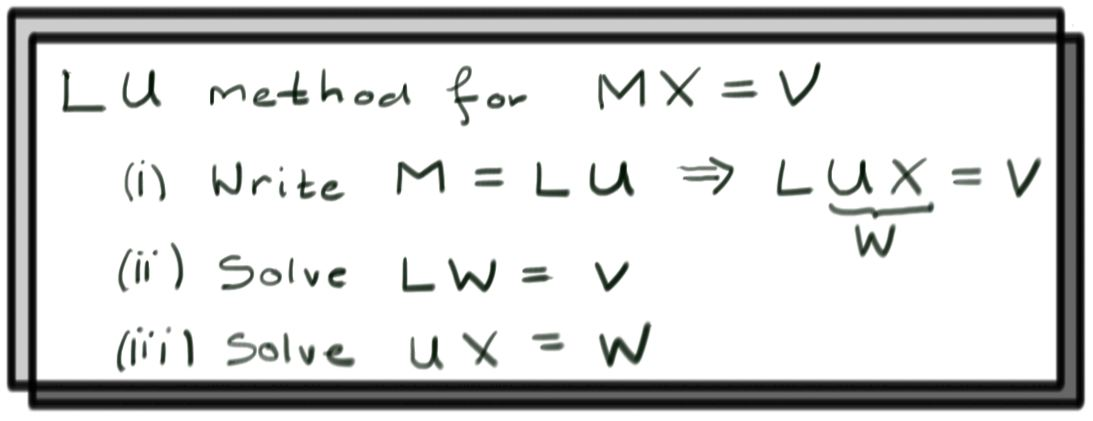
\includegraphics[scale=.3]{\luDecompPath/LU_solution.jpg}
\end{center}
%\end{figure}

\section{Finding an $LU$ Decomposition.}
\label{finding_LU_decomp}
 
For any given matrix, there are actually many different $LU$ decompositions.  However, there is a unique $LU$ decomposition in which the $L$ matrix has ones on the diagonal. In that case $L$ is called a \emph{lower unit triangular matrix}\index{Lower unit triangular matrix}.

To find the $LU$ decomposition, we'll create two sequences of matrices $L_0, L_1, \ldots$ and $U_0, U_1, \ldots$ such that at each step, $L_iU_i=M$.  Each of the $L_i$ will be lower triangular, but only the last $U_i$ will be upper triangular.

Start by setting $L_0=I$ and $U_0=M$, because $L_0U_0=M$. A main concept of this calculation is captured by the following example:

\begin{example}
Consider $$E=\begin{pmatrix}1&0\\\lambda&1\end{pmatrix}\, ,\qquad M=\begin{pmatrix}a&b&c&\cdots\\d&e&f&\cdots\end{pmatrix}\, .$$
Lets compute $EM$
$$
EM=\begin{pmatrix}a&b&c&\cdots\\d+\lambda a&e+\lambda b&f+\lambda c&\cdots\end{pmatrix}\, ,.
$$
Something neat happened here: multiplying $M$ by $E$ performed the row operation $R_2\to R_2+\lambda R-1$ on $M$.
Another interesting fact:
$$
E^{-1}:=\begin{pmatrix}1&0\\-\lambda&1\end{pmatrix}
$$ 
obeys (check this yourself...)
$$
E^{-1} E = 1\, .
$$
Hence $M=E^{-1} E M$ or, writing this out
$$
\begin{pmatrix}a&b&c&\cdots\\d&e&f&\cdots\end{pmatrix}=\begin{pmatrix}1&0\\-\lambda&1\end{pmatrix} \begin{pmatrix}a&b&c&\cdots\\d+\lambda a&e+\lambda b&f+\lambda c&\cdots\end{pmatrix}\, .
$$
Here the matrix on the left is lower triangular, while the matrix on the right has had a row operation performed on it.
\end{example}




\vspace{2mm}
We would like to  use the first row of $U_0$ to zero out the first entry of every row below it.  For our running example, $$U_0=M=\begin{pmatrix}
6 & 18 & 3 \\
2 & 12 & 1 \\
4 & 15 & 3 
\end{pmatrix}\, ,$$ so we would like to perform the row operations $R_2\to R_2 -\frac 13 R_1$ and $R_3\to R_3-\frac 23R_1$.
%so the second row minus $\frac{1}{3}$ of the first row will zero out the first entry in the second row.  Likewise, the third row minus $\frac{2}{3}$ of the first row will zero out the first entry in the third row.
If we perform these row operations on $U_0$ to produce 
$$U_1=\begin{pmatrix}
6 & 18 & 3 \\
0 & 6 & 0 \\
0 & 3 & 1 
\end{pmatrix}\, ,$$
we need to multiply this on the left by a lower triangular matrix $L_1$ so that the product $L_1U_1=M$ still.
The above example shows how to do this:
Set $L_1$ to be the lower triangular matrix whose first column is filled with the minus constants used to zero out the first column of $M$.  Then $$L_1 = \begin{pmatrix}
1 & 0 & 0 \\[1mm]
\frac{1}{3} & 1 & 0 \\[1mm]
\frac{2}{3} & 0 & 1 
\end{pmatrix}\, .$$  
%Set $U_1$ to be the matrix obtained by zeroing out the first column of $M$.  Then $U_1=\begin{pmatrix}
%6 & 18 & 3 \\
%0 & 6 & 0 \\
%0 & 3 & 1 
%\end{pmatrix}$.
By construction $L_1 U_1=M$, but you should compute this yourself as a double check.

Now repeat the process by zeroing the second column of $U_1$ below the diagonal using the second row of $U_1$ using the row operation
$R_3\to R_3-\frac 12 R_2$ to produce
$$U_2=\begin{pmatrix}6&18&3\\0&6&0\\0&0&1\end{pmatrix}\, .$$
The matrix that undoes this row operation is obtained in the same way we found $L_1$ above and is:
$$
\begin{pmatrix}
1&0&0\\
0&1&0\\
0&\frac 12& 0
\end{pmatrix}\, .
$$
Thus our answer for $L_2$ is the product of this matrix with $L_1$, namely
$$
L_2=
\begin{pmatrix}
1 & 0 & 0 \\[1mm]
\frac{1}{3} & 1 & 0 \\[1mm]
\frac{2}{3} & 0 & 1 
\end{pmatrix}\begin{pmatrix}
1&0&0\\
0&1&0\\
0&\frac 12& 0
\end{pmatrix}
=\begin{pmatrix}
1 & 0 & 0 \\[1mm]
\frac{1}{3} & 1 & 0 \\[1mm]
\frac{2}{3} & \frac{1}{2} & 1 
\end{pmatrix}\, .
$$
Notice that it is lower triangular because 

\begin{center}
\textcolor{brown}{THE PRODUCT OF LOWER TRIANGULAR MATRICES IS ALWAYS LOWER TRIANGULAR!}
\end{center}

\noindent
Moreover it is obtained by recording minus the constants used for all our row operations in the appropriate columns (this always works this way).
Moreover, $U_2$ is upper triangular and $M=L_2U_2$, we are done!
Putting this all together we have
$$M=\begin{pmatrix}
6 & 18 & 3 \\
2 & 12 & 1 \\
4 & 15 & 3 
\end{pmatrix}= \begin{pmatrix}
1 & 0 & 0 \\[1mm]
\frac{1}{3} & 1 & 0 \\[1mm]
\frac{2}{3} & \frac{1}{2} & 1 
\end{pmatrix}\begin{pmatrix}
6 & 18 & 3 \\
0 & 6 & 0 \\
0 & 0 & 1 
\end{pmatrix}\, .$$  
%Since $U_2$ is upper-triangular, we're done.  Inserting the new number into $L_1$ to get $L_2$ really is safe: the numbers in the first column don't affect the second column of $U_1$, since the first column of $U_1$ is already zeroed out.

If the matrix you're working with has more than three rows, just continue this process by zeroing out the next column below the diagonal, and repeat until there's nothing left to do.

\videoscriptlink{lu_decomposition_example.mp4}{Another $LU$ decomposition example}{scripts_lu_decomposition_example}

The fractions in the $L$ matrix are admittedly ugly.  For two matrices $LU$, we can multiply one entire column of $L$ by a constant $\lambda$ and divide the corresponding row of $U$ by the same constant without changing the product of the two matrices.  Then:

\begin{eqnarray*}
LU &=& \begin{pmatrix}
1 & 0 & 0 \\[1mm]
\frac{1}{3} & 1 & 0 \\[1mm]
\frac{2}{3} & \frac{1}{2} & 1 
\end{pmatrix}
I
\begin{pmatrix}
6 & 18 & 3 \\
0 & 6 & 0 \\
0 & 0 & 1 
\end{pmatrix} \\
&=&
\begin{pmatrix}
1 & 0 & 0 \\[1mm]
\frac{1}{3} & 1 & 0 \\[1mm]
\frac{2}{3} & \frac{1}{2} & 1 
\end{pmatrix}
\begin{pmatrix}
3 & 0 & 0 \\
0 & 6 & 0 \\
0 & 0 & 1 
\end{pmatrix}
\begin{pmatrix}
\frac{1}{3} & 0 & 0 \\[1mm]
0 & \frac{1}{6} & 0 \\[1mm]
0 & 0 & 1 
\end{pmatrix}
\begin{pmatrix}
6 & 18 & 3 \\
0 & 6 & 0 \\
0 & 0 & 1 
\end{pmatrix} \\
&=&
\begin{pmatrix}
3 & 0 & 0 \\
1 & 6 & 0 \\
2 & 3 & 1 
\end{pmatrix}\begin{pmatrix}
2 & 6 & 1 \\
0 & 1 & 0 \\
0 & 0 & 1 
\end{pmatrix}.
\end{eqnarray*}
The resulting matrix looks nicer, but isn't in standard (lower unit triangular matrix) form.

\reading{11}{2}
%\href{\webworkurl ReadingHomework11/2/}{Reading homework: problem 11.2}

For matrices that are not square, $LU$ decomposition still makes sense.  Given an $m\times n$ matrix $M$, for example we could write $M=LU$ with $L$ a square lower unit triangular matrix, and $U$ a rectangular matrix.  Then $L$ will be an $m\times m$ matrix, and $U$ will be an $m\times n$ matrix (of the same shape as $M$).  From here, the process is exactly the same as for a square matrix.  We create a sequence of matrices $L_i$ and $U_i$ that is eventually the $LU$ decomposition.  Again, we start with $L_0=I$ and $U_0=M$.

\begin{example}
Let's find the $LU$ decomposition of $M=U_0=\begin{pmatrix}
-2 & 1 & 3 \\
-4 & 4 & 1 
\end{pmatrix}$.  Since $M$ is a $2\times 3$ matrix, our decomposition will consist of a $2\times 2$ matrix and a $2\times 3$ matrix.  Then we start with $L_0=I_2=\begin{pmatrix}
1 & 0 \\
0 & 1
\end{pmatrix}$.

The next step is to zero-out the first column of $M$ below the diagonal.  There is only one row to cancel, then, and it can be removed by subtracting $2$ times the first row of $M$ to the second row of $M$.  Then:

\[
L_1=\begin{pmatrix}
1 & 0 \\
2 & 1
\end{pmatrix}, \qquad 
U_1 = \begin{pmatrix}
-2 & 1 & 3 \\
0 & 2 & -5 
\end{pmatrix}
\]
Since $U_1$ is upper triangular, we're done.  With a larger matrix, we would just continue the process.
\end{example}





\section{Block $LDU$ Decomposition}

Let $M$ be a square block matrix with square blocks $X,Y,Z,W$ such that $X^{-1}$ exists.  Then $M$ can be decomposed as a block $LDU$ decomposition, where $D$ is block diagonal, as follows:
\[
M=\begin{pmatrix}
X & Y \\
Z & W
\end{pmatrix}
\]

Then: \[M=\begin{pmatrix}
I &  0 \\
ZX^{-1} & I
\end{pmatrix}\begin{pmatrix}
X & 0 \\
0 & W-ZX^{-1}Y
\end{pmatrix}\begin{pmatrix}
I & X^{-1}Y \\
0 & I
\end{pmatrix}.\]
This can be checked explicitly simply by block-multiplying these three matrices.

\videoscriptlink{lu_decomposition_blocks.mp4}{Block $LDU$ Explanation}{scripts_lu_decomposition_blocks}

\begin{example}
For a $2\times 2$ matrix, we can regard each entry as a block.
\[
\begin{pmatrix}
1 & 2 \\
3 & 4
\end{pmatrix}=
\begin{pmatrix}
1 & 0 \\
3 & 1
\end{pmatrix}
\begin{pmatrix}
1 & 0 \\
0 & -2
\end{pmatrix}
\begin{pmatrix}
1 & 2 \\
0 & 1
\end{pmatrix}
\]
By multiplying the diagonal matrix by the upper triangular matrix, we get the standard $LU$ decomposition of the matrix.
\end{example}


%\section*{References}
%Wikipedia:
%\begin{itemize}
%\item \href{http://en.wikipedia.org/wiki/LU_decomposition}{$LU$ Decomposition}
%\item \href{http://en.wikipedia.org/wiki/Block_LU_decomposition}{Block $LU$ Decomposition}
%\end{itemize}

\section{Review Problems}



\begin{enumerate}

\item Let $D=\begin{pmatrix}
\lambda_1 & \mc0 \\
\mc0 & \lambda_2 \\
\end{pmatrix}$.
\begin{enumerate}
\item Write $D$ in terms of the vectors $e_1$ and $e_2$, and their transposes.
\item Suppose $P=\begin{pmatrix}
a & b \\
c & d \\
\end{pmatrix}$ is invertible.  Show that $D$ is similar to
\[
M=\frac{1}{ad-bc}\begin{pmatrix}
\lambda_1ad-\lambda_2bc & -(\lambda_1-\lambda_2)ab \\[1mm]
(\lambda_1-\lambda_2)cd & -\lambda_1bc + \lambda_2ad
\end{pmatrix}.
\]
\item Suppose the vectors $\rowvec{a,b}$ and $\rowvec{c,d}$ are orthogonal.  What can you say about $M$ in this case? (Hint: think about what \(M^T\) is equal to.)
\end{enumerate}

\phantomnewpage

\item \label{orthogprob} Suppose $S=\{v_1, \ldots, v_n \}$ is an \emph{orthogonal} (not orthonormal) basis for~$\Re^n$.  Then we can write any vector $v$ as $v=\sum_ic^iv_i$ for some constants $c^i$.  Find a formula for the constants $c^i$ in terms of $v$ and the vectors in~$S$.

\Videoscriptlink{orthonormal_bases_hint.mp4}{Hint}{scripts_orthonormal_bases_hint}
\phantomnewpage

\item \label{orthogprojprob} Let $u,v$ be linearly independent vectors in $\Re^3$, and $P=\spa \{ u,v\}$ be the plane spanned by $u$ and $v$.  
\begin{enumerate}
\item Is the vector $v^\bot := v-\frac{u\cdot v}{u\cdot u}u$ in the plane $P$?
\item  What is the (cosine of the) angle between $v^\bot$ and $u$?
\item %Given your solution to the above, 
How can you find a third vector perpendicular to both $u$ and $v^\bot$?
\item  Construct an orthonormal basis for $\Re^3$ from $u$ and $v$.
\item  Test your abstract formul\ae\ starting with 
\[
u=\rowvec{1 , 2 , 0} \text{ and } v=\rowvec{0 , 1 , 1}.
\]
\end{enumerate}

\Videoscriptlink{orthonormal_bases_hint3.mp4}{Hint}{scripts_orthonormal_bases_hint3}

\phantomnewpage



\item Find an orthonormal  basis for $\Re^4$ which includes $(1,1,1,1)$ using the following procedure:\\
\begin{enumerate} 
\item Pick a vector perpendicular to the vector 
$$v_1 =\colvec{1\\1\\1\\1}$$ from the solution set of the matrix equation $$v_1^Tx=0\, .$$ Pick the vector $v_2$ obtained from the standard Gaussian elimination procedure which is the coefficient of $x_2$.
\item Pick a vector perpendicular to both $v_1$ and $v_2$ from the solutions set of the matrix equation $$\colvec{v_1^T\\[1mm]v_2^T}x=0\, .$$ Pick the vector $v_3$ obtained from the standard Gaussian elimination procedure with $x_3$ as the coefficient. 
\item Pick a vector perpendicular to $v_1,v_2,$ and $v_3$ from the solution set of the matrix equation $$\colvec{v_1^T\\[1mm]v_2^T\\[1mm]v_3^T}x=0\, .$$  Pick the vector $v_4$ obtained from the standard Gaussian elimination procedure with $x_3$ as the coefficient. 
\item Normalize the four vectors obtained   above.
\end{enumerate}


\item Use the inner product $$f\cdot g := \int_0^1 f(x)g(x)dx$$  on the vector space $V={\rm span} \{1,x,x^2,x^3\}$ to perform the Gram-Schmidt procedure on the set of vectors $\{1,x,x^2,x^3\}$. 

\item Use the inner product $$f\cdot g := \int_0^{2\pi} f(x)g(x)dx$$  on the vector space $V={\rm span} \{\sin(x),\sin(2x),\sin(3x) \}$ to perform the Gram-Schmidt procedure on the set of vectors $\{\sin(x),\sin(2x),\sin(3x) \}$. \\
Try to build an orthonormal basis for the vector space $$\spa \{ \sin(nx)~| ~n\in \N \}\, .$$
%What do you suspect about the vector space $\spa \{ \sin(nx)~| ~n\in \N \}$?\\
%What do you suspect about the vector space $\spa \{ \sin(ax)~|~ a \in \Re \}$?
\item 
\begin{enumerate}
\item
Show that if $Q$ is an orthogonal $n\times n$ matrix, then $$u\dotprod v = (Qu)\dotprod (Qv)\, ,$$ for any $u,v\in \Re^n$. That is, $Q$ preserves the inner product. 
\item Does $Q$ preserve the outer product? 
\item  If the set of vectors $\{ u_1,\dots,u_n\}$ is orthonormal and $\{ \lambda_1,\cdots,\lambda_n\}$ is a set of numbers, 
then what are the eigenvalues and eigenvectors of the matrix
$M=\sum_{i=1}^n \lambda_i u_i u_i^T$? 
\item How would the eigenvectors and eigenvalues of this matrix change if we replaced  $\{ u_1,\dots,u_n\}$ by $\{ Qu_1,\dots,Q u_n\}$?
\end{enumerate}


\item Carefully write out the Gram-Schmidt procedure for the set of vectors 
$$\left\{ \colvec{1\\1\\1}, \colvec{1\\-1\\1}, \colvec{1\\1\\-1} \right\} \, .$$ Is it possible to rescale the second vector obtained in the procedure to a vector with integer components? 


\item 
\label{basisortho}
\begin{enumerate}
\item Suppose $u$ and $v$ are linearly independent.  Show that $u$ and $v^\perp$ are also linearly independent.  Explain why $\{u, v^\perp\}$ is a basis for $\spa \{u,v\}$.



\Videoscriptlink{gram_schmidt_and_orthogonal_complements_hint.mp4}{Hint}{gram_schmidt_and_orthogonal_complements_hint}

\item Repeat the previous problem, but with three independent vectors $u,v,w$
 where $v^\perp$ and $w^\perp$ are as defined by the Gram-Schmidt procedure. 
\end{enumerate}

\phantomnewpage


\item \label{QRprob} Find the $QR$ factorization of
$$
M=\begin{pmatrix}1&0&\phantom{\!-}2\\-1&2&0\\-1&-2&2
\end{pmatrix}\, .
$$

\phantomnewpage

\item Given any three vectors $u,v,w$, when do $v^\perp$ or $w^\perp$ of the Gram--Schmidt procedure vanish?

\phantomnewpage

\item For $U$ a subspace of $W$, use the subspace theorem to check that $U^\perp$ is a subspace of $W$.

\phantomnewpage


\phantomnewpage

\item %(Extra Credit) 
Let $S_n$ and $A_n$ define the space of $n \times n$ symmetric and anti-symmetric matrices, respectively. These are subspaces of the vector space $M^n_n$ of all $n\times n$ matrices. What is $\dim M^n_n$, $\dim S_n$, and $\dim A_n$? Show that $M^n_n = S_n + A_n$. Define an inner product on square matrices
$$
M\cdot N ={\rm tr} MN\, .
$$
Is $A_n^{\perp}=S_n$? Is $M^n_n = S_n \oplus A_n$?

%\emph{Hint: Note that $\dim S_n = \dim U_n$ where $U_n$ is the vector space of all $n \times n$ upper triangular matrices, and also note that $\dim A_n = \dim \widetilde{U}_n$ where $\widetilde{U}_n$ is the vector space of all strictly $n \times n$ upper triangular matrices (\emph{i.e.} the diagonal entries are all 0).}

\item The vector space $V={\rm span} \{ \sin(t),\sin(2t), \sin(3t) , \sin(3t)\}$ has an inner product: 
$$f\cdot g:=\int _0^{2\pi}f(t)g(t) dt\, .$$ Find the orthogonal compliment to $U={\rm span} \{ \sin(t)+\sin(2t) \}$ in $V$. Express $\sin(t)-\sin(2t)$ as  the sum of vectors from $U$ and $U^\perp$.

\end{enumerate}

\phantomnewpage

\newpage
 %ch17 

\chapter{\luDecompTitle}
\label{LUdecomp}

Certain matrices are easier to work with than others.  In this section, we will see how to write any square\footnote{The case where $M$ is not square is dealt with at the end of the lecture.} matrix $M$ as the product of two simpler matrices.  We will write $$M=LU\, ,$$ where:
\begin{itemize}
\item $L$ is \emph{lower triangular}\index{Lower triangular matrix}.  This means that all entries above the main diagonal are zero.  In notation,
$L=(l^i_j)$ with $l^i_j=0$ for all $j>i$.
\[L=\begin{pmatrix}
l^1_1 & 0 & 0 & \cdots \\
l^2_1 & l^2_2 & 0 & \cdots \\
l^3_1 & l^3_2 & l^3_3 & \cdots \\
\vdots & \vdots & \vdots & \ddots \\
\end{pmatrix}
\]

\item $U$ is \emph{upper triangular}\index{Upper triangular matrix}.  This means that all entries below the main diagonal are zero.  In notation,
$U=(u^i_j)$ with $u^i_j=0$ for all $j<i$.
\[U=\begin{pmatrix}
u^1_1 & u^1_2 & u^1_3 & \cdots \\
0 & u^2_2 & u^2_3 & \cdots \\
0 & 0 & u^3_3 & \cdots \\
\vdots & \vdots & \vdots & \ddots \\
\end{pmatrix}
\]
\end{itemize}
$M=LU$ is called an \emph{$LU$ decomposition}\index{LU@$LU$ decomposition} of $M$.

This is a useful trick for  computational reasons; it is much easier to compute the inverse of an upper or lower triangular matrix than general matrices.  Since inverses are useful for solving linear systems, this makes solving any linear system associated to the matrix much faster as well.  The determinant---a very important quantity associated with any square matrix---is very easy to compute for triangular matrices.

\begin{example}
Linear systems associated to upper triangular matrices are very easy to solve by back substitution.
\[
\begin{amatrix}{2}
a & b & 1 \\
0 & c & e \\
\end{amatrix} \ \Rightarrow \ y=\frac{e}{c}\, , \quad x=\frac{1}{a}\left(1-\frac{be}{c}\right)
\]

\[
\begin{amatrix}{3}
1 & 0 & 0 & d \\
a & 1 & 0 & e \\
b & c & 1 & f \\
\end{amatrix} \Rightarrow x=d\, , \qquad y=e-ad\, , \qquad z=f-bd-c(e-ad)
\]
For lower triangular matrices, \emph{back} substitution\index{Back substitution} gives a quick solution; for upper triangular matrices, \emph{forward} substitution\index{Forward substitution} gives the solution.
\end{example}





\section{Using $LU$ Decomposition to Solve Linear Systems}

Suppose we have $M=LU$ and want to solve the system
\[
MX=LUX=V.
\]

\begin{itemize}
\item{Step 1:} Set $W=\colvec{u\\v\\w}=UX$.  

\item{Step 2:} Solve the system $LW=V$.  This should be simple by forward substitution since $L$ is lower triangular.  Suppose the solution to $LW=V$ is $W_0$.  

\item{Step 3:} Now solve the system $UX=W_0$.  This should be easy by backward substitution, since $U$ is upper triangular.  The solution to this system is the solution to the original system.
\end{itemize}
We can think of this as using the matrix $L$ to perform row operations on the matrix $U$ in order to solve the system; this idea also appears in the  study of determinants.

%\href{\webworkurl ReadingHomework11/1/}{Reading homework: problem 11.1}
\reading{11}{1}

\begin{example}
Consider the linear system:
\[
      \begin{linsys}{4}
            6x & +&18y & +&3z         &=& 3  \\[1mm]
            2x & +&12y & +&z	    &=& 19 \\[1mm]
            4x & +&15y & +&3z         &=& 0  
      \end{linsys}
\]

An $LU$ decomposition for the associated matrix $M$ is:
\[
\begin{pmatrix}
6 & 18 & 3 \\
2 & 12 & 1 \\
4 & 15 & 3 
\end{pmatrix} =
\begin{pmatrix}
3 & 0 & 0 \\
1 & 6 & 0 \\
2 & 3 & 1 
\end{pmatrix}
\begin{pmatrix}
2 & 6 & 1 \\
0 & 1 & 0 \\
0 & 0 & 1 
\end{pmatrix}.
\]

\begin{itemize}
\item{Step 1:} \hypertarget{LUproc}{Set} $W=\colvec{u\\v\\w}=UX$.  

\item{Step 2:} Solve the system $LW=V$:

\[
\begin{pmatrix}
3 & 0 & 0 \\
1 & 6 & 0 \\
2 & 3 & 1 
\end{pmatrix}
\colvec{u\\v\\w} =
\colvec{3\\19\\0}
\]

By substitution, we get $u=1$, $v=3$, and $w=-11$.  Then 
\[W_0=\colvec{1\\3\\-11}\]

\item{Step 3:} Solve the system $UX=W_0$.  
\[
\begin{pmatrix}
2 & 6 & 1 \\
0 & 1 & 0 \\
0 & 0 & 1 
\end{pmatrix}
\colvec{x\\y\\z} =
\colvec{1\\3\\-11}
\]
Back substitution gives $z=-11, y=3$, and $x=-3$.  

Then $X=\colvec{-3\\3\\-11}$, and we're done.
\end{itemize}
\end{example}

\videoscriptlink{lu_decomposition_using_lu_decomp.mp4}{Using a $LU$ decomposition}{scripts_lu_decomposition_using_lu_example}

%\begin{figure}
\begin{center}
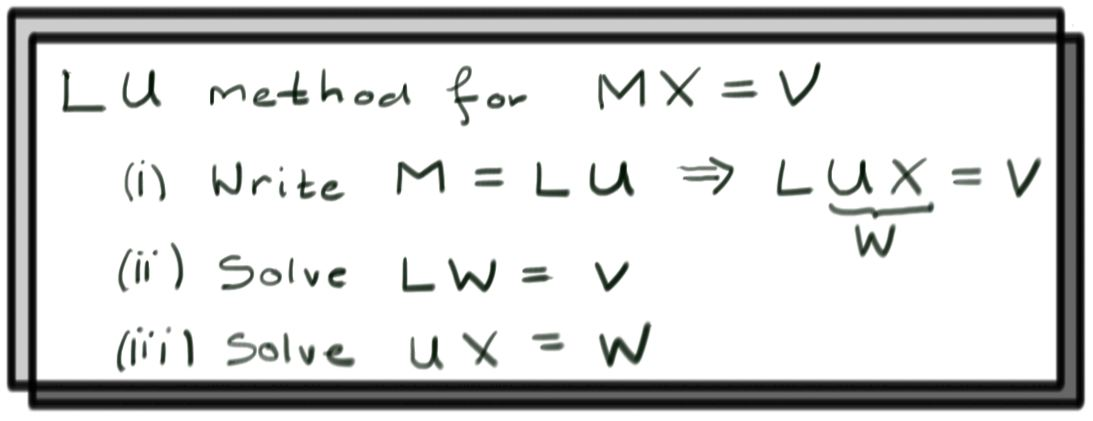
\includegraphics[scale=.3]{\luDecompPath/LU_solution.jpg}
\end{center}
%\end{figure}

\section{Finding an $LU$ Decomposition.}
\label{finding_LU_decomp}
 
For any given matrix, there are actually many different $LU$ decompositions.  However, there is a unique $LU$ decomposition in which the $L$ matrix has ones on the diagonal. In that case $L$ is called a \emph{lower unit triangular matrix}\index{Lower unit triangular matrix}.

To find the $LU$ decomposition, we'll create two sequences of matrices $L_0, L_1, \ldots$ and $U_0, U_1, \ldots$ such that at each step, $L_iU_i=M$.  Each of the $L_i$ will be lower triangular, but only the last $U_i$ will be upper triangular.

Start by setting $L_0=I$ and $U_0=M$, because $L_0U_0=M$. A main concept of this calculation is captured by the following example:

\begin{example}
Consider $$E=\begin{pmatrix}1&0\\\lambda&1\end{pmatrix}\, ,\qquad M=\begin{pmatrix}a&b&c&\cdots\\d&e&f&\cdots\end{pmatrix}\, .$$
Lets compute $EM$
$$
EM=\begin{pmatrix}a&b&c&\cdots\\d+\lambda a&e+\lambda b&f+\lambda c&\cdots\end{pmatrix}\, ,.
$$
Something neat happened here: multiplying $M$ by $E$ performed the row operation $R_2\to R_2+\lambda R-1$ on $M$.
Another interesting fact:
$$
E^{-1}:=\begin{pmatrix}1&0\\-\lambda&1\end{pmatrix}
$$ 
obeys (check this yourself...)
$$
E^{-1} E = 1\, .
$$
Hence $M=E^{-1} E M$ or, writing this out
$$
\begin{pmatrix}a&b&c&\cdots\\d&e&f&\cdots\end{pmatrix}=\begin{pmatrix}1&0\\-\lambda&1\end{pmatrix} \begin{pmatrix}a&b&c&\cdots\\d+\lambda a&e+\lambda b&f+\lambda c&\cdots\end{pmatrix}\, .
$$
Here the matrix on the left is lower triangular, while the matrix on the right has had a row operation performed on it.
\end{example}




\vspace{2mm}
We would like to  use the first row of $U_0$ to zero out the first entry of every row below it.  For our running example, $$U_0=M=\begin{pmatrix}
6 & 18 & 3 \\
2 & 12 & 1 \\
4 & 15 & 3 
\end{pmatrix}\, ,$$ so we would like to perform the row operations $R_2\to R_2 -\frac 13 R_1$ and $R_3\to R_3-\frac 23R_1$.
%so the second row minus $\frac{1}{3}$ of the first row will zero out the first entry in the second row.  Likewise, the third row minus $\frac{2}{3}$ of the first row will zero out the first entry in the third row.
If we perform these row operations on $U_0$ to produce 
$$U_1=\begin{pmatrix}
6 & 18 & 3 \\
0 & 6 & 0 \\
0 & 3 & 1 
\end{pmatrix}\, ,$$
we need to multiply this on the left by a lower triangular matrix $L_1$ so that the product $L_1U_1=M$ still.
The above example shows how to do this:
Set $L_1$ to be the lower triangular matrix whose first column is filled with the minus constants used to zero out the first column of $M$.  Then $$L_1 = \begin{pmatrix}
1 & 0 & 0 \\[1mm]
\frac{1}{3} & 1 & 0 \\[1mm]
\frac{2}{3} & 0 & 1 
\end{pmatrix}\, .$$  
%Set $U_1$ to be the matrix obtained by zeroing out the first column of $M$.  Then $U_1=\begin{pmatrix}
%6 & 18 & 3 \\
%0 & 6 & 0 \\
%0 & 3 & 1 
%\end{pmatrix}$.
By construction $L_1 U_1=M$, but you should compute this yourself as a double check.

Now repeat the process by zeroing the second column of $U_1$ below the diagonal using the second row of $U_1$ using the row operation
$R_3\to R_3-\frac 12 R_2$ to produce
$$U_2=\begin{pmatrix}6&18&3\\0&6&0\\0&0&1\end{pmatrix}\, .$$
The matrix that undoes this row operation is obtained in the same way we found $L_1$ above and is:
$$
\begin{pmatrix}
1&0&0\\
0&1&0\\
0&\frac 12& 0
\end{pmatrix}\, .
$$
Thus our answer for $L_2$ is the product of this matrix with $L_1$, namely
$$
L_2=
\begin{pmatrix}
1 & 0 & 0 \\[1mm]
\frac{1}{3} & 1 & 0 \\[1mm]
\frac{2}{3} & 0 & 1 
\end{pmatrix}\begin{pmatrix}
1&0&0\\
0&1&0\\
0&\frac 12& 0
\end{pmatrix}
=\begin{pmatrix}
1 & 0 & 0 \\[1mm]
\frac{1}{3} & 1 & 0 \\[1mm]
\frac{2}{3} & \frac{1}{2} & 1 
\end{pmatrix}\, .
$$
Notice that it is lower triangular because 

\begin{center}
\textcolor{brown}{THE PRODUCT OF LOWER TRIANGULAR MATRICES IS ALWAYS LOWER TRIANGULAR!}
\end{center}

\noindent
Moreover it is obtained by recording minus the constants used for all our row operations in the appropriate columns (this always works this way).
Moreover, $U_2$ is upper triangular and $M=L_2U_2$, we are done!
Putting this all together we have
$$M=\begin{pmatrix}
6 & 18 & 3 \\
2 & 12 & 1 \\
4 & 15 & 3 
\end{pmatrix}= \begin{pmatrix}
1 & 0 & 0 \\[1mm]
\frac{1}{3} & 1 & 0 \\[1mm]
\frac{2}{3} & \frac{1}{2} & 1 
\end{pmatrix}\begin{pmatrix}
6 & 18 & 3 \\
0 & 6 & 0 \\
0 & 0 & 1 
\end{pmatrix}\, .$$  
%Since $U_2$ is upper-triangular, we're done.  Inserting the new number into $L_1$ to get $L_2$ really is safe: the numbers in the first column don't affect the second column of $U_1$, since the first column of $U_1$ is already zeroed out.

If the matrix you're working with has more than three rows, just continue this process by zeroing out the next column below the diagonal, and repeat until there's nothing left to do.

\videoscriptlink{lu_decomposition_example.mp4}{Another $LU$ decomposition example}{scripts_lu_decomposition_example}

The fractions in the $L$ matrix are admittedly ugly.  For two matrices $LU$, we can multiply one entire column of $L$ by a constant $\lambda$ and divide the corresponding row of $U$ by the same constant without changing the product of the two matrices.  Then:

\begin{eqnarray*}
LU &=& \begin{pmatrix}
1 & 0 & 0 \\[1mm]
\frac{1}{3} & 1 & 0 \\[1mm]
\frac{2}{3} & \frac{1}{2} & 1 
\end{pmatrix}
I
\begin{pmatrix}
6 & 18 & 3 \\
0 & 6 & 0 \\
0 & 0 & 1 
\end{pmatrix} \\
&=&
\begin{pmatrix}
1 & 0 & 0 \\[1mm]
\frac{1}{3} & 1 & 0 \\[1mm]
\frac{2}{3} & \frac{1}{2} & 1 
\end{pmatrix}
\begin{pmatrix}
3 & 0 & 0 \\
0 & 6 & 0 \\
0 & 0 & 1 
\end{pmatrix}
\begin{pmatrix}
\frac{1}{3} & 0 & 0 \\[1mm]
0 & \frac{1}{6} & 0 \\[1mm]
0 & 0 & 1 
\end{pmatrix}
\begin{pmatrix}
6 & 18 & 3 \\
0 & 6 & 0 \\
0 & 0 & 1 
\end{pmatrix} \\
&=&
\begin{pmatrix}
3 & 0 & 0 \\
1 & 6 & 0 \\
2 & 3 & 1 
\end{pmatrix}\begin{pmatrix}
2 & 6 & 1 \\
0 & 1 & 0 \\
0 & 0 & 1 
\end{pmatrix}.
\end{eqnarray*}
The resulting matrix looks nicer, but isn't in standard (lower unit triangular matrix) form.

\reading{11}{2}
%\href{\webworkurl ReadingHomework11/2/}{Reading homework: problem 11.2}

For matrices that are not square, $LU$ decomposition still makes sense.  Given an $m\times n$ matrix $M$, for example we could write $M=LU$ with $L$ a square lower unit triangular matrix, and $U$ a rectangular matrix.  Then $L$ will be an $m\times m$ matrix, and $U$ will be an $m\times n$ matrix (of the same shape as $M$).  From here, the process is exactly the same as for a square matrix.  We create a sequence of matrices $L_i$ and $U_i$ that is eventually the $LU$ decomposition.  Again, we start with $L_0=I$ and $U_0=M$.

\begin{example}
Let's find the $LU$ decomposition of $M=U_0=\begin{pmatrix}
-2 & 1 & 3 \\
-4 & 4 & 1 
\end{pmatrix}$.  Since $M$ is a $2\times 3$ matrix, our decomposition will consist of a $2\times 2$ matrix and a $2\times 3$ matrix.  Then we start with $L_0=I_2=\begin{pmatrix}
1 & 0 \\
0 & 1
\end{pmatrix}$.

The next step is to zero-out the first column of $M$ below the diagonal.  There is only one row to cancel, then, and it can be removed by subtracting $2$ times the first row of $M$ to the second row of $M$.  Then:

\[
L_1=\begin{pmatrix}
1 & 0 \\
2 & 1
\end{pmatrix}, \qquad 
U_1 = \begin{pmatrix}
-2 & 1 & 3 \\
0 & 2 & -5 
\end{pmatrix}
\]
Since $U_1$ is upper triangular, we're done.  With a larger matrix, we would just continue the process.
\end{example}





\section{Block $LDU$ Decomposition}

Let $M$ be a square block matrix with square blocks $X,Y,Z,W$ such that $X^{-1}$ exists.  Then $M$ can be decomposed as a block $LDU$ decomposition, where $D$ is block diagonal, as follows:
\[
M=\begin{pmatrix}
X & Y \\
Z & W
\end{pmatrix}
\]

Then: \[M=\begin{pmatrix}
I &  0 \\
ZX^{-1} & I
\end{pmatrix}\begin{pmatrix}
X & 0 \\
0 & W-ZX^{-1}Y
\end{pmatrix}\begin{pmatrix}
I & X^{-1}Y \\
0 & I
\end{pmatrix}.\]
This can be checked explicitly simply by block-multiplying these three matrices.

\videoscriptlink{lu_decomposition_blocks.mp4}{Block $LDU$ Explanation}{scripts_lu_decomposition_blocks}

\begin{example}
For a $2\times 2$ matrix, we can regard each entry as a block.
\[
\begin{pmatrix}
1 & 2 \\
3 & 4
\end{pmatrix}=
\begin{pmatrix}
1 & 0 \\
3 & 1
\end{pmatrix}
\begin{pmatrix}
1 & 0 \\
0 & -2
\end{pmatrix}
\begin{pmatrix}
1 & 2 \\
0 & 1
\end{pmatrix}
\]
By multiplying the diagonal matrix by the upper triangular matrix, we get the standard $LU$ decomposition of the matrix.
\end{example}


%\section*{References}
%Wikipedia:
%\begin{itemize}
%\item \href{http://en.wikipedia.org/wiki/LU_decomposition}{$LU$ Decomposition}
%\item \href{http://en.wikipedia.org/wiki/Block_LU_decomposition}{Block $LU$ Decomposition}
%\end{itemize}

\section{Review Problems}



\begin{enumerate}

\item Let $D=\begin{pmatrix}
\lambda_1 & \mc0 \\
\mc0 & \lambda_2 \\
\end{pmatrix}$.
\begin{enumerate}
\item Write $D$ in terms of the vectors $e_1$ and $e_2$, and their transposes.
\item Suppose $P=\begin{pmatrix}
a & b \\
c & d \\
\end{pmatrix}$ is invertible.  Show that $D$ is similar to
\[
M=\frac{1}{ad-bc}\begin{pmatrix}
\lambda_1ad-\lambda_2bc & -(\lambda_1-\lambda_2)ab \\[1mm]
(\lambda_1-\lambda_2)cd & -\lambda_1bc + \lambda_2ad
\end{pmatrix}.
\]
\item Suppose the vectors $\rowvec{a,b}$ and $\rowvec{c,d}$ are orthogonal.  What can you say about $M$ in this case? (Hint: think about what \(M^T\) is equal to.)
\end{enumerate}

\phantomnewpage

\item \label{orthogprob} Suppose $S=\{v_1, \ldots, v_n \}$ is an \emph{orthogonal} (not orthonormal) basis for~$\Re^n$.  Then we can write any vector $v$ as $v=\sum_ic^iv_i$ for some constants $c^i$.  Find a formula for the constants $c^i$ in terms of $v$ and the vectors in~$S$.

\Videoscriptlink{orthonormal_bases_hint.mp4}{Hint}{scripts_orthonormal_bases_hint}
\phantomnewpage

\item \label{orthogprojprob} Let $u,v$ be linearly independent vectors in $\Re^3$, and $P=\spa \{ u,v\}$ be the plane spanned by $u$ and $v$.  
\begin{enumerate}
\item Is the vector $v^\bot := v-\frac{u\cdot v}{u\cdot u}u$ in the plane $P$?
\item  What is the (cosine of the) angle between $v^\bot$ and $u$?
\item %Given your solution to the above, 
How can you find a third vector perpendicular to both $u$ and $v^\bot$?
\item  Construct an orthonormal basis for $\Re^3$ from $u$ and $v$.
\item  Test your abstract formul\ae\ starting with 
\[
u=\rowvec{1 , 2 , 0} \text{ and } v=\rowvec{0 , 1 , 1}.
\]
\end{enumerate}

\Videoscriptlink{orthonormal_bases_hint3.mp4}{Hint}{scripts_orthonormal_bases_hint3}

\phantomnewpage



\item Find an orthonormal  basis for $\Re^4$ which includes $(1,1,1,1)$ using the following procedure:\\
\begin{enumerate} 
\item Pick a vector perpendicular to the vector 
$$v_1 =\colvec{1\\1\\1\\1}$$ from the solution set of the matrix equation $$v_1^Tx=0\, .$$ Pick the vector $v_2$ obtained from the standard Gaussian elimination procedure which is the coefficient of $x_2$.
\item Pick a vector perpendicular to both $v_1$ and $v_2$ from the solutions set of the matrix equation $$\colvec{v_1^T\\[1mm]v_2^T}x=0\, .$$ Pick the vector $v_3$ obtained from the standard Gaussian elimination procedure with $x_3$ as the coefficient. 
\item Pick a vector perpendicular to $v_1,v_2,$ and $v_3$ from the solution set of the matrix equation $$\colvec{v_1^T\\[1mm]v_2^T\\[1mm]v_3^T}x=0\, .$$  Pick the vector $v_4$ obtained from the standard Gaussian elimination procedure with $x_3$ as the coefficient. 
\item Normalize the four vectors obtained   above.
\end{enumerate}


\item Use the inner product $$f\cdot g := \int_0^1 f(x)g(x)dx$$  on the vector space $V={\rm span} \{1,x,x^2,x^3\}$ to perform the Gram-Schmidt procedure on the set of vectors $\{1,x,x^2,x^3\}$. 

\item Use the inner product $$f\cdot g := \int_0^{2\pi} f(x)g(x)dx$$  on the vector space $V={\rm span} \{\sin(x),\sin(2x),\sin(3x) \}$ to perform the Gram-Schmidt procedure on the set of vectors $\{\sin(x),\sin(2x),\sin(3x) \}$. \\
Try to build an orthonormal basis for the vector space $$\spa \{ \sin(nx)~| ~n\in \N \}\, .$$
%What do you suspect about the vector space $\spa \{ \sin(nx)~| ~n\in \N \}$?\\
%What do you suspect about the vector space $\spa \{ \sin(ax)~|~ a \in \Re \}$?
\item 
\begin{enumerate}
\item
Show that if $Q$ is an orthogonal $n\times n$ matrix, then $$u\dotprod v = (Qu)\dotprod (Qv)\, ,$$ for any $u,v\in \Re^n$. That is, $Q$ preserves the inner product. 
\item Does $Q$ preserve the outer product? 
\item  If the set of vectors $\{ u_1,\dots,u_n\}$ is orthonormal and $\{ \lambda_1,\cdots,\lambda_n\}$ is a set of numbers, 
then what are the eigenvalues and eigenvectors of the matrix
$M=\sum_{i=1}^n \lambda_i u_i u_i^T$? 
\item How would the eigenvectors and eigenvalues of this matrix change if we replaced  $\{ u_1,\dots,u_n\}$ by $\{ Qu_1,\dots,Q u_n\}$?
\end{enumerate}


\item Carefully write out the Gram-Schmidt procedure for the set of vectors 
$$\left\{ \colvec{1\\1\\1}, \colvec{1\\-1\\1}, \colvec{1\\1\\-1} \right\} \, .$$ Is it possible to rescale the second vector obtained in the procedure to a vector with integer components? 


\item 
\label{basisortho}
\begin{enumerate}
\item Suppose $u$ and $v$ are linearly independent.  Show that $u$ and $v^\perp$ are also linearly independent.  Explain why $\{u, v^\perp\}$ is a basis for $\spa \{u,v\}$.



\Videoscriptlink{gram_schmidt_and_orthogonal_complements_hint.mp4}{Hint}{gram_schmidt_and_orthogonal_complements_hint}

\item Repeat the previous problem, but with three independent vectors $u,v,w$
 where $v^\perp$ and $w^\perp$ are as defined by the Gram-Schmidt procedure. 
\end{enumerate}

\phantomnewpage


\item \label{QRprob} Find the $QR$ factorization of
$$
M=\begin{pmatrix}1&0&\phantom{\!-}2\\-1&2&0\\-1&-2&2
\end{pmatrix}\, .
$$

\phantomnewpage

\item Given any three vectors $u,v,w$, when do $v^\perp$ or $w^\perp$ of the Gram--Schmidt procedure vanish?

\phantomnewpage

\item For $U$ a subspace of $W$, use the subspace theorem to check that $U^\perp$ is a subspace of $W$.

\phantomnewpage


\phantomnewpage

\item %(Extra Credit) 
Let $S_n$ and $A_n$ define the space of $n \times n$ symmetric and anti-symmetric matrices, respectively. These are subspaces of the vector space $M^n_n$ of all $n\times n$ matrices. What is $\dim M^n_n$, $\dim S_n$, and $\dim A_n$? Show that $M^n_n = S_n + A_n$. Define an inner product on square matrices
$$
M\cdot N ={\rm tr} MN\, .
$$
Is $A_n^{\perp}=S_n$? Is $M^n_n = S_n \oplus A_n$?

%\emph{Hint: Note that $\dim S_n = \dim U_n$ where $U_n$ is the vector space of all $n \times n$ upper triangular matrices, and also note that $\dim A_n = \dim \widetilde{U}_n$ where $\widetilde{U}_n$ is the vector space of all strictly $n \times n$ upper triangular matrices (\emph{i.e.} the diagonal entries are all 0).}

\item The vector space $V={\rm span} \{ \sin(t),\sin(2t), \sin(3t) , \sin(3t)\}$ has an inner product: 
$$f\cdot g:=\int _0^{2\pi}f(t)g(t) dt\, .$$ Find the orthogonal compliment to $U={\rm span} \{ \sin(t)+\sin(2t) \}$ in $V$. Express $\sin(t)-\sin(2t)$ as  the sum of vectors from $U$ and $U^\perp$.

\end{enumerate}

\phantomnewpage

\newpage


\chapter{\luDecompTitle}
\label{LUdecomp}

Certain matrices are easier to work with than others.  In this section, we will see how to write any square\footnote{The case where $M$ is not square is dealt with at the end of the lecture.} matrix $M$ as the product of two simpler matrices.  We will write $$M=LU\, ,$$ where:
\begin{itemize}
\item $L$ is \emph{lower triangular}\index{Lower triangular matrix}.  This means that all entries above the main diagonal are zero.  In notation,
$L=(l^i_j)$ with $l^i_j=0$ for all $j>i$.
\[L=\begin{pmatrix}
l^1_1 & 0 & 0 & \cdots \\
l^2_1 & l^2_2 & 0 & \cdots \\
l^3_1 & l^3_2 & l^3_3 & \cdots \\
\vdots & \vdots & \vdots & \ddots \\
\end{pmatrix}
\]

\item $U$ is \emph{upper triangular}\index{Upper triangular matrix}.  This means that all entries below the main diagonal are zero.  In notation,
$U=(u^i_j)$ with $u^i_j=0$ for all $j<i$.
\[U=\begin{pmatrix}
u^1_1 & u^1_2 & u^1_3 & \cdots \\
0 & u^2_2 & u^2_3 & \cdots \\
0 & 0 & u^3_3 & \cdots \\
\vdots & \vdots & \vdots & \ddots \\
\end{pmatrix}
\]
\end{itemize}
$M=LU$ is called an \emph{$LU$ decomposition}\index{LU@$LU$ decomposition} of $M$.

This is a useful trick for  computational reasons; it is much easier to compute the inverse of an upper or lower triangular matrix than general matrices.  Since inverses are useful for solving linear systems, this makes solving any linear system associated to the matrix much faster as well.  The determinant---a very important quantity associated with any square matrix---is very easy to compute for triangular matrices.

\begin{example}
Linear systems associated to upper triangular matrices are very easy to solve by back substitution.
\[
\begin{amatrix}{2}
a & b & 1 \\
0 & c & e \\
\end{amatrix} \ \Rightarrow \ y=\frac{e}{c}\, , \quad x=\frac{1}{a}\left(1-\frac{be}{c}\right)
\]

\[
\begin{amatrix}{3}
1 & 0 & 0 & d \\
a & 1 & 0 & e \\
b & c & 1 & f \\
\end{amatrix} \Rightarrow x=d\, , \qquad y=e-ad\, , \qquad z=f-bd-c(e-ad)
\]
For lower triangular matrices, \emph{back} substitution\index{Back substitution} gives a quick solution; for upper triangular matrices, \emph{forward} substitution\index{Forward substitution} gives the solution.
\end{example}





\section{Using $LU$ Decomposition to Solve Linear Systems}

Suppose we have $M=LU$ and want to solve the system
\[
MX=LUX=V.
\]

\begin{itemize}
\item{Step 1:} Set $W=\colvec{u\\v\\w}=UX$.  

\item{Step 2:} Solve the system $LW=V$.  This should be simple by forward substitution since $L$ is lower triangular.  Suppose the solution to $LW=V$ is $W_0$.  

\item{Step 3:} Now solve the system $UX=W_0$.  This should be easy by backward substitution, since $U$ is upper triangular.  The solution to this system is the solution to the original system.
\end{itemize}
We can think of this as using the matrix $L$ to perform row operations on the matrix $U$ in order to solve the system; this idea also appears in the  study of determinants.

%\href{\webworkurl ReadingHomework11/1/}{Reading homework: problem 11.1}
\reading{11}{1}

\begin{example}
Consider the linear system:
\[
      \begin{linsys}{4}
            6x & +&18y & +&3z         &=& 3  \\[1mm]
            2x & +&12y & +&z	    &=& 19 \\[1mm]
            4x & +&15y & +&3z         &=& 0  
      \end{linsys}
\]

An $LU$ decomposition for the associated matrix $M$ is:
\[
\begin{pmatrix}
6 & 18 & 3 \\
2 & 12 & 1 \\
4 & 15 & 3 
\end{pmatrix} =
\begin{pmatrix}
3 & 0 & 0 \\
1 & 6 & 0 \\
2 & 3 & 1 
\end{pmatrix}
\begin{pmatrix}
2 & 6 & 1 \\
0 & 1 & 0 \\
0 & 0 & 1 
\end{pmatrix}.
\]

\begin{itemize}
\item{Step 1:} \hypertarget{LUproc}{Set} $W=\colvec{u\\v\\w}=UX$.  

\item{Step 2:} Solve the system $LW=V$:

\[
\begin{pmatrix}
3 & 0 & 0 \\
1 & 6 & 0 \\
2 & 3 & 1 
\end{pmatrix}
\colvec{u\\v\\w} =
\colvec{3\\19\\0}
\]

By substitution, we get $u=1$, $v=3$, and $w=-11$.  Then 
\[W_0=\colvec{1\\3\\-11}\]

\item{Step 3:} Solve the system $UX=W_0$.  
\[
\begin{pmatrix}
2 & 6 & 1 \\
0 & 1 & 0 \\
0 & 0 & 1 
\end{pmatrix}
\colvec{x\\y\\z} =
\colvec{1\\3\\-11}
\]
Back substitution gives $z=-11, y=3$, and $x=-3$.  

Then $X=\colvec{-3\\3\\-11}$, and we're done.
\end{itemize}
\end{example}

\videoscriptlink{lu_decomposition_using_lu_decomp.mp4}{Using a $LU$ decomposition}{scripts_lu_decomposition_using_lu_example}

%\begin{figure}
\begin{center}
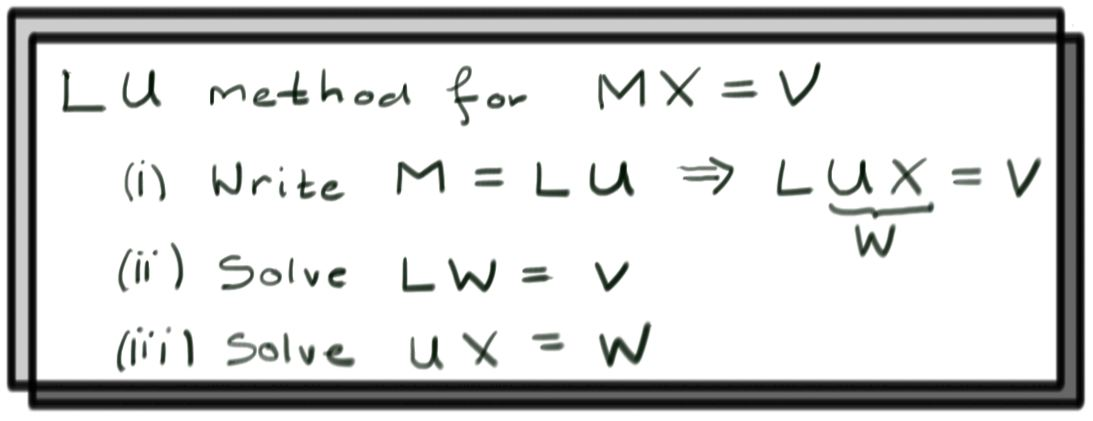
\includegraphics[scale=.3]{\luDecompPath/LU_solution.jpg}
\end{center}
%\end{figure}

\section{Finding an $LU$ Decomposition.}
\label{finding_LU_decomp}
 
For any given matrix, there are actually many different $LU$ decompositions.  However, there is a unique $LU$ decomposition in which the $L$ matrix has ones on the diagonal. In that case $L$ is called a \emph{lower unit triangular matrix}\index{Lower unit triangular matrix}.

To find the $LU$ decomposition, we'll create two sequences of matrices $L_0, L_1, \ldots$ and $U_0, U_1, \ldots$ such that at each step, $L_iU_i=M$.  Each of the $L_i$ will be lower triangular, but only the last $U_i$ will be upper triangular.

Start by setting $L_0=I$ and $U_0=M$, because $L_0U_0=M$. A main concept of this calculation is captured by the following example:

\begin{example}
Consider $$E=\begin{pmatrix}1&0\\\lambda&1\end{pmatrix}\, ,\qquad M=\begin{pmatrix}a&b&c&\cdots\\d&e&f&\cdots\end{pmatrix}\, .$$
Lets compute $EM$
$$
EM=\begin{pmatrix}a&b&c&\cdots\\d+\lambda a&e+\lambda b&f+\lambda c&\cdots\end{pmatrix}\, ,.
$$
Something neat happened here: multiplying $M$ by $E$ performed the row operation $R_2\to R_2+\lambda R-1$ on $M$.
Another interesting fact:
$$
E^{-1}:=\begin{pmatrix}1&0\\-\lambda&1\end{pmatrix}
$$ 
obeys (check this yourself...)
$$
E^{-1} E = 1\, .
$$
Hence $M=E^{-1} E M$ or, writing this out
$$
\begin{pmatrix}a&b&c&\cdots\\d&e&f&\cdots\end{pmatrix}=\begin{pmatrix}1&0\\-\lambda&1\end{pmatrix} \begin{pmatrix}a&b&c&\cdots\\d+\lambda a&e+\lambda b&f+\lambda c&\cdots\end{pmatrix}\, .
$$
Here the matrix on the left is lower triangular, while the matrix on the right has had a row operation performed on it.
\end{example}




\vspace{2mm}
We would like to  use the first row of $U_0$ to zero out the first entry of every row below it.  For our running example, $$U_0=M=\begin{pmatrix}
6 & 18 & 3 \\
2 & 12 & 1 \\
4 & 15 & 3 
\end{pmatrix}\, ,$$ so we would like to perform the row operations $R_2\to R_2 -\frac 13 R_1$ and $R_3\to R_3-\frac 23R_1$.
%so the second row minus $\frac{1}{3}$ of the first row will zero out the first entry in the second row.  Likewise, the third row minus $\frac{2}{3}$ of the first row will zero out the first entry in the third row.
If we perform these row operations on $U_0$ to produce 
$$U_1=\begin{pmatrix}
6 & 18 & 3 \\
0 & 6 & 0 \\
0 & 3 & 1 
\end{pmatrix}\, ,$$
we need to multiply this on the left by a lower triangular matrix $L_1$ so that the product $L_1U_1=M$ still.
The above example shows how to do this:
Set $L_1$ to be the lower triangular matrix whose first column is filled with the minus constants used to zero out the first column of $M$.  Then $$L_1 = \begin{pmatrix}
1 & 0 & 0 \\[1mm]
\frac{1}{3} & 1 & 0 \\[1mm]
\frac{2}{3} & 0 & 1 
\end{pmatrix}\, .$$  
%Set $U_1$ to be the matrix obtained by zeroing out the first column of $M$.  Then $U_1=\begin{pmatrix}
%6 & 18 & 3 \\
%0 & 6 & 0 \\
%0 & 3 & 1 
%\end{pmatrix}$.
By construction $L_1 U_1=M$, but you should compute this yourself as a double check.

Now repeat the process by zeroing the second column of $U_1$ below the diagonal using the second row of $U_1$ using the row operation
$R_3\to R_3-\frac 12 R_2$ to produce
$$U_2=\begin{pmatrix}6&18&3\\0&6&0\\0&0&1\end{pmatrix}\, .$$
The matrix that undoes this row operation is obtained in the same way we found $L_1$ above and is:
$$
\begin{pmatrix}
1&0&0\\
0&1&0\\
0&\frac 12& 0
\end{pmatrix}\, .
$$
Thus our answer for $L_2$ is the product of this matrix with $L_1$, namely
$$
L_2=
\begin{pmatrix}
1 & 0 & 0 \\[1mm]
\frac{1}{3} & 1 & 0 \\[1mm]
\frac{2}{3} & 0 & 1 
\end{pmatrix}\begin{pmatrix}
1&0&0\\
0&1&0\\
0&\frac 12& 0
\end{pmatrix}
=\begin{pmatrix}
1 & 0 & 0 \\[1mm]
\frac{1}{3} & 1 & 0 \\[1mm]
\frac{2}{3} & \frac{1}{2} & 1 
\end{pmatrix}\, .
$$
Notice that it is lower triangular because 

\begin{center}
\textcolor{brown}{THE PRODUCT OF LOWER TRIANGULAR MATRICES IS ALWAYS LOWER TRIANGULAR!}
\end{center}

\noindent
Moreover it is obtained by recording minus the constants used for all our row operations in the appropriate columns (this always works this way).
Moreover, $U_2$ is upper triangular and $M=L_2U_2$, we are done!
Putting this all together we have
$$M=\begin{pmatrix}
6 & 18 & 3 \\
2 & 12 & 1 \\
4 & 15 & 3 
\end{pmatrix}= \begin{pmatrix}
1 & 0 & 0 \\[1mm]
\frac{1}{3} & 1 & 0 \\[1mm]
\frac{2}{3} & \frac{1}{2} & 1 
\end{pmatrix}\begin{pmatrix}
6 & 18 & 3 \\
0 & 6 & 0 \\
0 & 0 & 1 
\end{pmatrix}\, .$$  
%Since $U_2$ is upper-triangular, we're done.  Inserting the new number into $L_1$ to get $L_2$ really is safe: the numbers in the first column don't affect the second column of $U_1$, since the first column of $U_1$ is already zeroed out.

If the matrix you're working with has more than three rows, just continue this process by zeroing out the next column below the diagonal, and repeat until there's nothing left to do.

\videoscriptlink{lu_decomposition_example.mp4}{Another $LU$ decomposition example}{scripts_lu_decomposition_example}

The fractions in the $L$ matrix are admittedly ugly.  For two matrices $LU$, we can multiply one entire column of $L$ by a constant $\lambda$ and divide the corresponding row of $U$ by the same constant without changing the product of the two matrices.  Then:

\begin{eqnarray*}
LU &=& \begin{pmatrix}
1 & 0 & 0 \\[1mm]
\frac{1}{3} & 1 & 0 \\[1mm]
\frac{2}{3} & \frac{1}{2} & 1 
\end{pmatrix}
I
\begin{pmatrix}
6 & 18 & 3 \\
0 & 6 & 0 \\
0 & 0 & 1 
\end{pmatrix} \\
&=&
\begin{pmatrix}
1 & 0 & 0 \\[1mm]
\frac{1}{3} & 1 & 0 \\[1mm]
\frac{2}{3} & \frac{1}{2} & 1 
\end{pmatrix}
\begin{pmatrix}
3 & 0 & 0 \\
0 & 6 & 0 \\
0 & 0 & 1 
\end{pmatrix}
\begin{pmatrix}
\frac{1}{3} & 0 & 0 \\[1mm]
0 & \frac{1}{6} & 0 \\[1mm]
0 & 0 & 1 
\end{pmatrix}
\begin{pmatrix}
6 & 18 & 3 \\
0 & 6 & 0 \\
0 & 0 & 1 
\end{pmatrix} \\
&=&
\begin{pmatrix}
3 & 0 & 0 \\
1 & 6 & 0 \\
2 & 3 & 1 
\end{pmatrix}\begin{pmatrix}
2 & 6 & 1 \\
0 & 1 & 0 \\
0 & 0 & 1 
\end{pmatrix}.
\end{eqnarray*}
The resulting matrix looks nicer, but isn't in standard (lower unit triangular matrix) form.

\reading{11}{2}
%\href{\webworkurl ReadingHomework11/2/}{Reading homework: problem 11.2}

For matrices that are not square, $LU$ decomposition still makes sense.  Given an $m\times n$ matrix $M$, for example we could write $M=LU$ with $L$ a square lower unit triangular matrix, and $U$ a rectangular matrix.  Then $L$ will be an $m\times m$ matrix, and $U$ will be an $m\times n$ matrix (of the same shape as $M$).  From here, the process is exactly the same as for a square matrix.  We create a sequence of matrices $L_i$ and $U_i$ that is eventually the $LU$ decomposition.  Again, we start with $L_0=I$ and $U_0=M$.

\begin{example}
Let's find the $LU$ decomposition of $M=U_0=\begin{pmatrix}
-2 & 1 & 3 \\
-4 & 4 & 1 
\end{pmatrix}$.  Since $M$ is a $2\times 3$ matrix, our decomposition will consist of a $2\times 2$ matrix and a $2\times 3$ matrix.  Then we start with $L_0=I_2=\begin{pmatrix}
1 & 0 \\
0 & 1
\end{pmatrix}$.

The next step is to zero-out the first column of $M$ below the diagonal.  There is only one row to cancel, then, and it can be removed by subtracting $2$ times the first row of $M$ to the second row of $M$.  Then:

\[
L_1=\begin{pmatrix}
1 & 0 \\
2 & 1
\end{pmatrix}, \qquad 
U_1 = \begin{pmatrix}
-2 & 1 & 3 \\
0 & 2 & -5 
\end{pmatrix}
\]
Since $U_1$ is upper triangular, we're done.  With a larger matrix, we would just continue the process.
\end{example}





\section{Block $LDU$ Decomposition}

Let $M$ be a square block matrix with square blocks $X,Y,Z,W$ such that $X^{-1}$ exists.  Then $M$ can be decomposed as a block $LDU$ decomposition, where $D$ is block diagonal, as follows:
\[
M=\begin{pmatrix}
X & Y \\
Z & W
\end{pmatrix}
\]

Then: \[M=\begin{pmatrix}
I &  0 \\
ZX^{-1} & I
\end{pmatrix}\begin{pmatrix}
X & 0 \\
0 & W-ZX^{-1}Y
\end{pmatrix}\begin{pmatrix}
I & X^{-1}Y \\
0 & I
\end{pmatrix}.\]
This can be checked explicitly simply by block-multiplying these three matrices.

\videoscriptlink{lu_decomposition_blocks.mp4}{Block $LDU$ Explanation}{scripts_lu_decomposition_blocks}

\begin{example}
For a $2\times 2$ matrix, we can regard each entry as a block.
\[
\begin{pmatrix}
1 & 2 \\
3 & 4
\end{pmatrix}=
\begin{pmatrix}
1 & 0 \\
3 & 1
\end{pmatrix}
\begin{pmatrix}
1 & 0 \\
0 & -2
\end{pmatrix}
\begin{pmatrix}
1 & 2 \\
0 & 1
\end{pmatrix}
\]
By multiplying the diagonal matrix by the upper triangular matrix, we get the standard $LU$ decomposition of the matrix.
\end{example}


%\section*{References}
%Wikipedia:
%\begin{itemize}
%\item \href{http://en.wikipedia.org/wiki/LU_decomposition}{$LU$ Decomposition}
%\item \href{http://en.wikipedia.org/wiki/Block_LU_decomposition}{Block $LU$ Decomposition}
%\end{itemize}

\section{Review Problems}



\begin{enumerate}

\item Let $D=\begin{pmatrix}
\lambda_1 & \mc0 \\
\mc0 & \lambda_2 \\
\end{pmatrix}$.
\begin{enumerate}
\item Write $D$ in terms of the vectors $e_1$ and $e_2$, and their transposes.
\item Suppose $P=\begin{pmatrix}
a & b \\
c & d \\
\end{pmatrix}$ is invertible.  Show that $D$ is similar to
\[
M=\frac{1}{ad-bc}\begin{pmatrix}
\lambda_1ad-\lambda_2bc & -(\lambda_1-\lambda_2)ab \\[1mm]
(\lambda_1-\lambda_2)cd & -\lambda_1bc + \lambda_2ad
\end{pmatrix}.
\]
\item Suppose the vectors $\rowvec{a,b}$ and $\rowvec{c,d}$ are orthogonal.  What can you say about $M$ in this case? (Hint: think about what \(M^T\) is equal to.)
\end{enumerate}

\phantomnewpage

\item \label{orthogprob} Suppose $S=\{v_1, \ldots, v_n \}$ is an \emph{orthogonal} (not orthonormal) basis for~$\Re^n$.  Then we can write any vector $v$ as $v=\sum_ic^iv_i$ for some constants $c^i$.  Find a formula for the constants $c^i$ in terms of $v$ and the vectors in~$S$.

\Videoscriptlink{orthonormal_bases_hint.mp4}{Hint}{scripts_orthonormal_bases_hint}
\phantomnewpage

\item \label{orthogprojprob} Let $u,v$ be linearly independent vectors in $\Re^3$, and $P=\spa \{ u,v\}$ be the plane spanned by $u$ and $v$.  
\begin{enumerate}
\item Is the vector $v^\bot := v-\frac{u\cdot v}{u\cdot u}u$ in the plane $P$?
\item  What is the (cosine of the) angle between $v^\bot$ and $u$?
\item %Given your solution to the above, 
How can you find a third vector perpendicular to both $u$ and $v^\bot$?
\item  Construct an orthonormal basis for $\Re^3$ from $u$ and $v$.
\item  Test your abstract formul\ae\ starting with 
\[
u=\rowvec{1 , 2 , 0} \text{ and } v=\rowvec{0 , 1 , 1}.
\]
\end{enumerate}

\Videoscriptlink{orthonormal_bases_hint3.mp4}{Hint}{scripts_orthonormal_bases_hint3}

\phantomnewpage



\item Find an orthonormal  basis for $\Re^4$ which includes $(1,1,1,1)$ using the following procedure:\\
\begin{enumerate} 
\item Pick a vector perpendicular to the vector 
$$v_1 =\colvec{1\\1\\1\\1}$$ from the solution set of the matrix equation $$v_1^Tx=0\, .$$ Pick the vector $v_2$ obtained from the standard Gaussian elimination procedure which is the coefficient of $x_2$.
\item Pick a vector perpendicular to both $v_1$ and $v_2$ from the solutions set of the matrix equation $$\colvec{v_1^T\\[1mm]v_2^T}x=0\, .$$ Pick the vector $v_3$ obtained from the standard Gaussian elimination procedure with $x_3$ as the coefficient. 
\item Pick a vector perpendicular to $v_1,v_2,$ and $v_3$ from the solution set of the matrix equation $$\colvec{v_1^T\\[1mm]v_2^T\\[1mm]v_3^T}x=0\, .$$  Pick the vector $v_4$ obtained from the standard Gaussian elimination procedure with $x_3$ as the coefficient. 
\item Normalize the four vectors obtained   above.
\end{enumerate}


\item Use the inner product $$f\cdot g := \int_0^1 f(x)g(x)dx$$  on the vector space $V={\rm span} \{1,x,x^2,x^3\}$ to perform the Gram-Schmidt procedure on the set of vectors $\{1,x,x^2,x^3\}$. 

\item Use the inner product $$f\cdot g := \int_0^{2\pi} f(x)g(x)dx$$  on the vector space $V={\rm span} \{\sin(x),\sin(2x),\sin(3x) \}$ to perform the Gram-Schmidt procedure on the set of vectors $\{\sin(x),\sin(2x),\sin(3x) \}$. \\
Try to build an orthonormal basis for the vector space $$\spa \{ \sin(nx)~| ~n\in \N \}\, .$$
%What do you suspect about the vector space $\spa \{ \sin(nx)~| ~n\in \N \}$?\\
%What do you suspect about the vector space $\spa \{ \sin(ax)~|~ a \in \Re \}$?
\item 
\begin{enumerate}
\item
Show that if $Q$ is an orthogonal $n\times n$ matrix, then $$u\dotprod v = (Qu)\dotprod (Qv)\, ,$$ for any $u,v\in \Re^n$. That is, $Q$ preserves the inner product. 
\item Does $Q$ preserve the outer product? 
\item  If the set of vectors $\{ u_1,\dots,u_n\}$ is orthonormal and $\{ \lambda_1,\cdots,\lambda_n\}$ is a set of numbers, 
then what are the eigenvalues and eigenvectors of the matrix
$M=\sum_{i=1}^n \lambda_i u_i u_i^T$? 
\item How would the eigenvectors and eigenvalues of this matrix change if we replaced  $\{ u_1,\dots,u_n\}$ by $\{ Qu_1,\dots,Q u_n\}$?
\end{enumerate}


\item Carefully write out the Gram-Schmidt procedure for the set of vectors 
$$\left\{ \colvec{1\\1\\1}, \colvec{1\\-1\\1}, \colvec{1\\1\\-1} \right\} \, .$$ Is it possible to rescale the second vector obtained in the procedure to a vector with integer components? 


\item 
\label{basisortho}
\begin{enumerate}
\item Suppose $u$ and $v$ are linearly independent.  Show that $u$ and $v^\perp$ are also linearly independent.  Explain why $\{u, v^\perp\}$ is a basis for $\spa \{u,v\}$.



\Videoscriptlink{gram_schmidt_and_orthogonal_complements_hint.mp4}{Hint}{gram_schmidt_and_orthogonal_complements_hint}

\item Repeat the previous problem, but with three independent vectors $u,v,w$
 where $v^\perp$ and $w^\perp$ are as defined by the Gram-Schmidt procedure. 
\end{enumerate}

\phantomnewpage


\item \label{QRprob} Find the $QR$ factorization of
$$
M=\begin{pmatrix}1&0&\phantom{\!-}2\\-1&2&0\\-1&-2&2
\end{pmatrix}\, .
$$

\phantomnewpage

\item Given any three vectors $u,v,w$, when do $v^\perp$ or $w^\perp$ of the Gram--Schmidt procedure vanish?

\phantomnewpage

\item For $U$ a subspace of $W$, use the subspace theorem to check that $U^\perp$ is a subspace of $W$.

\phantomnewpage


\phantomnewpage

\item %(Extra Credit) 
Let $S_n$ and $A_n$ define the space of $n \times n$ symmetric and anti-symmetric matrices, respectively. These are subspaces of the vector space $M^n_n$ of all $n\times n$ matrices. What is $\dim M^n_n$, $\dim S_n$, and $\dim A_n$? Show that $M^n_n = S_n + A_n$. Define an inner product on square matrices
$$
M\cdot N ={\rm tr} MN\, .
$$
Is $A_n^{\perp}=S_n$? Is $M^n_n = S_n \oplus A_n$?

%\emph{Hint: Note that $\dim S_n = \dim U_n$ where $U_n$ is the vector space of all $n \times n$ upper triangular matrices, and also note that $\dim A_n = \dim \widetilde{U}_n$ where $\widetilde{U}_n$ is the vector space of all strictly $n \times n$ upper triangular matrices (\emph{i.e.} the diagonal entries are all 0).}

\item The vector space $V={\rm span} \{ \sin(t),\sin(2t), \sin(3t) , \sin(3t)\}$ has an inner product: 
$$f\cdot g:=\int _0^{2\pi}f(t)g(t) dt\, .$$ Find the orthogonal compliment to $U={\rm span} \{ \sin(t)+\sin(2t) \}$ in $V$. Express $\sin(t)-\sin(2t)$ as  the sum of vectors from $U$ and $U^\perp$.

\end{enumerate}

\phantomnewpage

\newpage


\chapter{\luDecompTitle}
\label{LUdecomp}

Certain matrices are easier to work with than others.  In this section, we will see how to write any square\footnote{The case where $M$ is not square is dealt with at the end of the lecture.} matrix $M$ as the product of two simpler matrices.  We will write $$M=LU\, ,$$ where:
\begin{itemize}
\item $L$ is \emph{lower triangular}\index{Lower triangular matrix}.  This means that all entries above the main diagonal are zero.  In notation,
$L=(l^i_j)$ with $l^i_j=0$ for all $j>i$.
\[L=\begin{pmatrix}
l^1_1 & 0 & 0 & \cdots \\
l^2_1 & l^2_2 & 0 & \cdots \\
l^3_1 & l^3_2 & l^3_3 & \cdots \\
\vdots & \vdots & \vdots & \ddots \\
\end{pmatrix}
\]

\item $U$ is \emph{upper triangular}\index{Upper triangular matrix}.  This means that all entries below the main diagonal are zero.  In notation,
$U=(u^i_j)$ with $u^i_j=0$ for all $j<i$.
\[U=\begin{pmatrix}
u^1_1 & u^1_2 & u^1_3 & \cdots \\
0 & u^2_2 & u^2_3 & \cdots \\
0 & 0 & u^3_3 & \cdots \\
\vdots & \vdots & \vdots & \ddots \\
\end{pmatrix}
\]
\end{itemize}
$M=LU$ is called an \emph{$LU$ decomposition}\index{LU@$LU$ decomposition} of $M$.

This is a useful trick for  computational reasons; it is much easier to compute the inverse of an upper or lower triangular matrix than general matrices.  Since inverses are useful for solving linear systems, this makes solving any linear system associated to the matrix much faster as well.  The determinant---a very important quantity associated with any square matrix---is very easy to compute for triangular matrices.

\begin{example}
Linear systems associated to upper triangular matrices are very easy to solve by back substitution.
\[
\begin{amatrix}{2}
a & b & 1 \\
0 & c & e \\
\end{amatrix} \ \Rightarrow \ y=\frac{e}{c}\, , \quad x=\frac{1}{a}\left(1-\frac{be}{c}\right)
\]

\[
\begin{amatrix}{3}
1 & 0 & 0 & d \\
a & 1 & 0 & e \\
b & c & 1 & f \\
\end{amatrix} \Rightarrow x=d\, , \qquad y=e-ad\, , \qquad z=f-bd-c(e-ad)
\]
For lower triangular matrices, \emph{back} substitution\index{Back substitution} gives a quick solution; for upper triangular matrices, \emph{forward} substitution\index{Forward substitution} gives the solution.
\end{example}





\section{Using $LU$ Decomposition to Solve Linear Systems}

Suppose we have $M=LU$ and want to solve the system
\[
MX=LUX=V.
\]

\begin{itemize}
\item{Step 1:} Set $W=\colvec{u\\v\\w}=UX$.  

\item{Step 2:} Solve the system $LW=V$.  This should be simple by forward substitution since $L$ is lower triangular.  Suppose the solution to $LW=V$ is $W_0$.  

\item{Step 3:} Now solve the system $UX=W_0$.  This should be easy by backward substitution, since $U$ is upper triangular.  The solution to this system is the solution to the original system.
\end{itemize}
We can think of this as using the matrix $L$ to perform row operations on the matrix $U$ in order to solve the system; this idea also appears in the  study of determinants.

%\href{\webworkurl ReadingHomework11/1/}{Reading homework: problem 11.1}
\reading{11}{1}

\begin{example}
Consider the linear system:
\[
      \begin{linsys}{4}
            6x & +&18y & +&3z         &=& 3  \\[1mm]
            2x & +&12y & +&z	    &=& 19 \\[1mm]
            4x & +&15y & +&3z         &=& 0  
      \end{linsys}
\]

An $LU$ decomposition for the associated matrix $M$ is:
\[
\begin{pmatrix}
6 & 18 & 3 \\
2 & 12 & 1 \\
4 & 15 & 3 
\end{pmatrix} =
\begin{pmatrix}
3 & 0 & 0 \\
1 & 6 & 0 \\
2 & 3 & 1 
\end{pmatrix}
\begin{pmatrix}
2 & 6 & 1 \\
0 & 1 & 0 \\
0 & 0 & 1 
\end{pmatrix}.
\]

\begin{itemize}
\item{Step 1:} \hypertarget{LUproc}{Set} $W=\colvec{u\\v\\w}=UX$.  

\item{Step 2:} Solve the system $LW=V$:

\[
\begin{pmatrix}
3 & 0 & 0 \\
1 & 6 & 0 \\
2 & 3 & 1 
\end{pmatrix}
\colvec{u\\v\\w} =
\colvec{3\\19\\0}
\]

By substitution, we get $u=1$, $v=3$, and $w=-11$.  Then 
\[W_0=\colvec{1\\3\\-11}\]

\item{Step 3:} Solve the system $UX=W_0$.  
\[
\begin{pmatrix}
2 & 6 & 1 \\
0 & 1 & 0 \\
0 & 0 & 1 
\end{pmatrix}
\colvec{x\\y\\z} =
\colvec{1\\3\\-11}
\]
Back substitution gives $z=-11, y=3$, and $x=-3$.  

Then $X=\colvec{-3\\3\\-11}$, and we're done.
\end{itemize}
\end{example}

\videoscriptlink{lu_decomposition_using_lu_decomp.mp4}{Using a $LU$ decomposition}{scripts_lu_decomposition_using_lu_example}

%\begin{figure}
\begin{center}
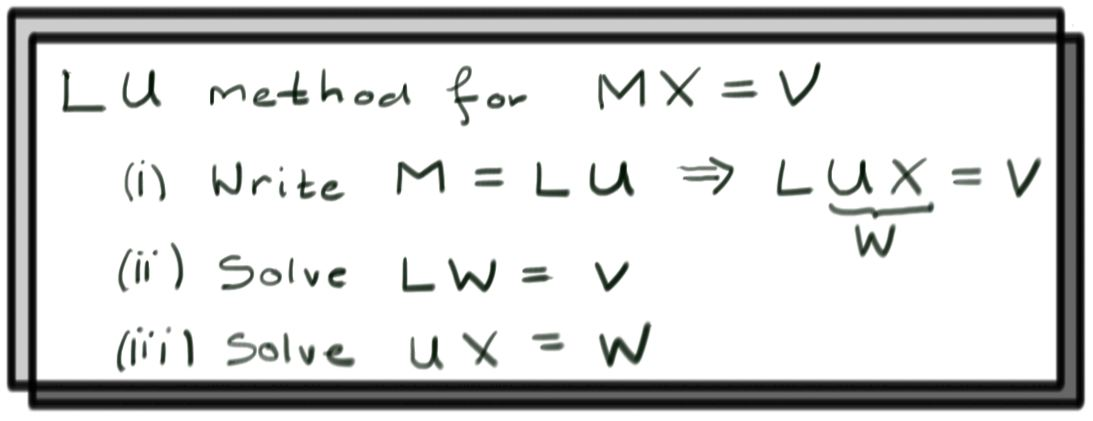
\includegraphics[scale=.3]{\luDecompPath/LU_solution.jpg}
\end{center}
%\end{figure}

\section{Finding an $LU$ Decomposition.}
\label{finding_LU_decomp}
 
For any given matrix, there are actually many different $LU$ decompositions.  However, there is a unique $LU$ decomposition in which the $L$ matrix has ones on the diagonal. In that case $L$ is called a \emph{lower unit triangular matrix}\index{Lower unit triangular matrix}.

To find the $LU$ decomposition, we'll create two sequences of matrices $L_0, L_1, \ldots$ and $U_0, U_1, \ldots$ such that at each step, $L_iU_i=M$.  Each of the $L_i$ will be lower triangular, but only the last $U_i$ will be upper triangular.

Start by setting $L_0=I$ and $U_0=M$, because $L_0U_0=M$. A main concept of this calculation is captured by the following example:

\begin{example}
Consider $$E=\begin{pmatrix}1&0\\\lambda&1\end{pmatrix}\, ,\qquad M=\begin{pmatrix}a&b&c&\cdots\\d&e&f&\cdots\end{pmatrix}\, .$$
Lets compute $EM$
$$
EM=\begin{pmatrix}a&b&c&\cdots\\d+\lambda a&e+\lambda b&f+\lambda c&\cdots\end{pmatrix}\, ,.
$$
Something neat happened here: multiplying $M$ by $E$ performed the row operation $R_2\to R_2+\lambda R-1$ on $M$.
Another interesting fact:
$$
E^{-1}:=\begin{pmatrix}1&0\\-\lambda&1\end{pmatrix}
$$ 
obeys (check this yourself...)
$$
E^{-1} E = 1\, .
$$
Hence $M=E^{-1} E M$ or, writing this out
$$
\begin{pmatrix}a&b&c&\cdots\\d&e&f&\cdots\end{pmatrix}=\begin{pmatrix}1&0\\-\lambda&1\end{pmatrix} \begin{pmatrix}a&b&c&\cdots\\d+\lambda a&e+\lambda b&f+\lambda c&\cdots\end{pmatrix}\, .
$$
Here the matrix on the left is lower triangular, while the matrix on the right has had a row operation performed on it.
\end{example}




\vspace{2mm}
We would like to  use the first row of $U_0$ to zero out the first entry of every row below it.  For our running example, $$U_0=M=\begin{pmatrix}
6 & 18 & 3 \\
2 & 12 & 1 \\
4 & 15 & 3 
\end{pmatrix}\, ,$$ so we would like to perform the row operations $R_2\to R_2 -\frac 13 R_1$ and $R_3\to R_3-\frac 23R_1$.
%so the second row minus $\frac{1}{3}$ of the first row will zero out the first entry in the second row.  Likewise, the third row minus $\frac{2}{3}$ of the first row will zero out the first entry in the third row.
If we perform these row operations on $U_0$ to produce 
$$U_1=\begin{pmatrix}
6 & 18 & 3 \\
0 & 6 & 0 \\
0 & 3 & 1 
\end{pmatrix}\, ,$$
we need to multiply this on the left by a lower triangular matrix $L_1$ so that the product $L_1U_1=M$ still.
The above example shows how to do this:
Set $L_1$ to be the lower triangular matrix whose first column is filled with the minus constants used to zero out the first column of $M$.  Then $$L_1 = \begin{pmatrix}
1 & 0 & 0 \\[1mm]
\frac{1}{3} & 1 & 0 \\[1mm]
\frac{2}{3} & 0 & 1 
\end{pmatrix}\, .$$  
%Set $U_1$ to be the matrix obtained by zeroing out the first column of $M$.  Then $U_1=\begin{pmatrix}
%6 & 18 & 3 \\
%0 & 6 & 0 \\
%0 & 3 & 1 
%\end{pmatrix}$.
By construction $L_1 U_1=M$, but you should compute this yourself as a double check.

Now repeat the process by zeroing the second column of $U_1$ below the diagonal using the second row of $U_1$ using the row operation
$R_3\to R_3-\frac 12 R_2$ to produce
$$U_2=\begin{pmatrix}6&18&3\\0&6&0\\0&0&1\end{pmatrix}\, .$$
The matrix that undoes this row operation is obtained in the same way we found $L_1$ above and is:
$$
\begin{pmatrix}
1&0&0\\
0&1&0\\
0&\frac 12& 0
\end{pmatrix}\, .
$$
Thus our answer for $L_2$ is the product of this matrix with $L_1$, namely
$$
L_2=
\begin{pmatrix}
1 & 0 & 0 \\[1mm]
\frac{1}{3} & 1 & 0 \\[1mm]
\frac{2}{3} & 0 & 1 
\end{pmatrix}\begin{pmatrix}
1&0&0\\
0&1&0\\
0&\frac 12& 0
\end{pmatrix}
=\begin{pmatrix}
1 & 0 & 0 \\[1mm]
\frac{1}{3} & 1 & 0 \\[1mm]
\frac{2}{3} & \frac{1}{2} & 1 
\end{pmatrix}\, .
$$
Notice that it is lower triangular because 

\begin{center}
\textcolor{brown}{THE PRODUCT OF LOWER TRIANGULAR MATRICES IS ALWAYS LOWER TRIANGULAR!}
\end{center}

\noindent
Moreover it is obtained by recording minus the constants used for all our row operations in the appropriate columns (this always works this way).
Moreover, $U_2$ is upper triangular and $M=L_2U_2$, we are done!
Putting this all together we have
$$M=\begin{pmatrix}
6 & 18 & 3 \\
2 & 12 & 1 \\
4 & 15 & 3 
\end{pmatrix}= \begin{pmatrix}
1 & 0 & 0 \\[1mm]
\frac{1}{3} & 1 & 0 \\[1mm]
\frac{2}{3} & \frac{1}{2} & 1 
\end{pmatrix}\begin{pmatrix}
6 & 18 & 3 \\
0 & 6 & 0 \\
0 & 0 & 1 
\end{pmatrix}\, .$$  
%Since $U_2$ is upper-triangular, we're done.  Inserting the new number into $L_1$ to get $L_2$ really is safe: the numbers in the first column don't affect the second column of $U_1$, since the first column of $U_1$ is already zeroed out.

If the matrix you're working with has more than three rows, just continue this process by zeroing out the next column below the diagonal, and repeat until there's nothing left to do.

\videoscriptlink{lu_decomposition_example.mp4}{Another $LU$ decomposition example}{scripts_lu_decomposition_example}

The fractions in the $L$ matrix are admittedly ugly.  For two matrices $LU$, we can multiply one entire column of $L$ by a constant $\lambda$ and divide the corresponding row of $U$ by the same constant without changing the product of the two matrices.  Then:

\begin{eqnarray*}
LU &=& \begin{pmatrix}
1 & 0 & 0 \\[1mm]
\frac{1}{3} & 1 & 0 \\[1mm]
\frac{2}{3} & \frac{1}{2} & 1 
\end{pmatrix}
I
\begin{pmatrix}
6 & 18 & 3 \\
0 & 6 & 0 \\
0 & 0 & 1 
\end{pmatrix} \\
&=&
\begin{pmatrix}
1 & 0 & 0 \\[1mm]
\frac{1}{3} & 1 & 0 \\[1mm]
\frac{2}{3} & \frac{1}{2} & 1 
\end{pmatrix}
\begin{pmatrix}
3 & 0 & 0 \\
0 & 6 & 0 \\
0 & 0 & 1 
\end{pmatrix}
\begin{pmatrix}
\frac{1}{3} & 0 & 0 \\[1mm]
0 & \frac{1}{6} & 0 \\[1mm]
0 & 0 & 1 
\end{pmatrix}
\begin{pmatrix}
6 & 18 & 3 \\
0 & 6 & 0 \\
0 & 0 & 1 
\end{pmatrix} \\
&=&
\begin{pmatrix}
3 & 0 & 0 \\
1 & 6 & 0 \\
2 & 3 & 1 
\end{pmatrix}\begin{pmatrix}
2 & 6 & 1 \\
0 & 1 & 0 \\
0 & 0 & 1 
\end{pmatrix}.
\end{eqnarray*}
The resulting matrix looks nicer, but isn't in standard (lower unit triangular matrix) form.

\reading{11}{2}
%\href{\webworkurl ReadingHomework11/2/}{Reading homework: problem 11.2}

For matrices that are not square, $LU$ decomposition still makes sense.  Given an $m\times n$ matrix $M$, for example we could write $M=LU$ with $L$ a square lower unit triangular matrix, and $U$ a rectangular matrix.  Then $L$ will be an $m\times m$ matrix, and $U$ will be an $m\times n$ matrix (of the same shape as $M$).  From here, the process is exactly the same as for a square matrix.  We create a sequence of matrices $L_i$ and $U_i$ that is eventually the $LU$ decomposition.  Again, we start with $L_0=I$ and $U_0=M$.

\begin{example}
Let's find the $LU$ decomposition of $M=U_0=\begin{pmatrix}
-2 & 1 & 3 \\
-4 & 4 & 1 
\end{pmatrix}$.  Since $M$ is a $2\times 3$ matrix, our decomposition will consist of a $2\times 2$ matrix and a $2\times 3$ matrix.  Then we start with $L_0=I_2=\begin{pmatrix}
1 & 0 \\
0 & 1
\end{pmatrix}$.

The next step is to zero-out the first column of $M$ below the diagonal.  There is only one row to cancel, then, and it can be removed by subtracting $2$ times the first row of $M$ to the second row of $M$.  Then:

\[
L_1=\begin{pmatrix}
1 & 0 \\
2 & 1
\end{pmatrix}, \qquad 
U_1 = \begin{pmatrix}
-2 & 1 & 3 \\
0 & 2 & -5 
\end{pmatrix}
\]
Since $U_1$ is upper triangular, we're done.  With a larger matrix, we would just continue the process.
\end{example}





\section{Block $LDU$ Decomposition}

Let $M$ be a square block matrix with square blocks $X,Y,Z,W$ such that $X^{-1}$ exists.  Then $M$ can be decomposed as a block $LDU$ decomposition, where $D$ is block diagonal, as follows:
\[
M=\begin{pmatrix}
X & Y \\
Z & W
\end{pmatrix}
\]

Then: \[M=\begin{pmatrix}
I &  0 \\
ZX^{-1} & I
\end{pmatrix}\begin{pmatrix}
X & 0 \\
0 & W-ZX^{-1}Y
\end{pmatrix}\begin{pmatrix}
I & X^{-1}Y \\
0 & I
\end{pmatrix}.\]
This can be checked explicitly simply by block-multiplying these three matrices.

\videoscriptlink{lu_decomposition_blocks.mp4}{Block $LDU$ Explanation}{scripts_lu_decomposition_blocks}

\begin{example}
For a $2\times 2$ matrix, we can regard each entry as a block.
\[
\begin{pmatrix}
1 & 2 \\
3 & 4
\end{pmatrix}=
\begin{pmatrix}
1 & 0 \\
3 & 1
\end{pmatrix}
\begin{pmatrix}
1 & 0 \\
0 & -2
\end{pmatrix}
\begin{pmatrix}
1 & 2 \\
0 & 1
\end{pmatrix}
\]
By multiplying the diagonal matrix by the upper triangular matrix, we get the standard $LU$ decomposition of the matrix.
\end{example}


%\section*{References}
%Wikipedia:
%\begin{itemize}
%\item \href{http://en.wikipedia.org/wiki/LU_decomposition}{$LU$ Decomposition}
%\item \href{http://en.wikipedia.org/wiki/Block_LU_decomposition}{Block $LU$ Decomposition}
%\end{itemize}

\section{Review Problems}



\begin{enumerate}

\item Let $D=\begin{pmatrix}
\lambda_1 & \mc0 \\
\mc0 & \lambda_2 \\
\end{pmatrix}$.
\begin{enumerate}
\item Write $D$ in terms of the vectors $e_1$ and $e_2$, and their transposes.
\item Suppose $P=\begin{pmatrix}
a & b \\
c & d \\
\end{pmatrix}$ is invertible.  Show that $D$ is similar to
\[
M=\frac{1}{ad-bc}\begin{pmatrix}
\lambda_1ad-\lambda_2bc & -(\lambda_1-\lambda_2)ab \\[1mm]
(\lambda_1-\lambda_2)cd & -\lambda_1bc + \lambda_2ad
\end{pmatrix}.
\]
\item Suppose the vectors $\rowvec{a,b}$ and $\rowvec{c,d}$ are orthogonal.  What can you say about $M$ in this case? (Hint: think about what \(M^T\) is equal to.)
\end{enumerate}

\phantomnewpage

\item \label{orthogprob} Suppose $S=\{v_1, \ldots, v_n \}$ is an \emph{orthogonal} (not orthonormal) basis for~$\Re^n$.  Then we can write any vector $v$ as $v=\sum_ic^iv_i$ for some constants $c^i$.  Find a formula for the constants $c^i$ in terms of $v$ and the vectors in~$S$.

\Videoscriptlink{orthonormal_bases_hint.mp4}{Hint}{scripts_orthonormal_bases_hint}
\phantomnewpage

\item \label{orthogprojprob} Let $u,v$ be linearly independent vectors in $\Re^3$, and $P=\spa \{ u,v\}$ be the plane spanned by $u$ and $v$.  
\begin{enumerate}
\item Is the vector $v^\bot := v-\frac{u\cdot v}{u\cdot u}u$ in the plane $P$?
\item  What is the (cosine of the) angle between $v^\bot$ and $u$?
\item %Given your solution to the above, 
How can you find a third vector perpendicular to both $u$ and $v^\bot$?
\item  Construct an orthonormal basis for $\Re^3$ from $u$ and $v$.
\item  Test your abstract formul\ae\ starting with 
\[
u=\rowvec{1 , 2 , 0} \text{ and } v=\rowvec{0 , 1 , 1}.
\]
\end{enumerate}

\Videoscriptlink{orthonormal_bases_hint3.mp4}{Hint}{scripts_orthonormal_bases_hint3}

\phantomnewpage



\item Find an orthonormal  basis for $\Re^4$ which includes $(1,1,1,1)$ using the following procedure:\\
\begin{enumerate} 
\item Pick a vector perpendicular to the vector 
$$v_1 =\colvec{1\\1\\1\\1}$$ from the solution set of the matrix equation $$v_1^Tx=0\, .$$ Pick the vector $v_2$ obtained from the standard Gaussian elimination procedure which is the coefficient of $x_2$.
\item Pick a vector perpendicular to both $v_1$ and $v_2$ from the solutions set of the matrix equation $$\colvec{v_1^T\\[1mm]v_2^T}x=0\, .$$ Pick the vector $v_3$ obtained from the standard Gaussian elimination procedure with $x_3$ as the coefficient. 
\item Pick a vector perpendicular to $v_1,v_2,$ and $v_3$ from the solution set of the matrix equation $$\colvec{v_1^T\\[1mm]v_2^T\\[1mm]v_3^T}x=0\, .$$  Pick the vector $v_4$ obtained from the standard Gaussian elimination procedure with $x_3$ as the coefficient. 
\item Normalize the four vectors obtained   above.
\end{enumerate}


\item Use the inner product $$f\cdot g := \int_0^1 f(x)g(x)dx$$  on the vector space $V={\rm span} \{1,x,x^2,x^3\}$ to perform the Gram-Schmidt procedure on the set of vectors $\{1,x,x^2,x^3\}$. 

\item Use the inner product $$f\cdot g := \int_0^{2\pi} f(x)g(x)dx$$  on the vector space $V={\rm span} \{\sin(x),\sin(2x),\sin(3x) \}$ to perform the Gram-Schmidt procedure on the set of vectors $\{\sin(x),\sin(2x),\sin(3x) \}$. \\
Try to build an orthonormal basis for the vector space $$\spa \{ \sin(nx)~| ~n\in \N \}\, .$$
%What do you suspect about the vector space $\spa \{ \sin(nx)~| ~n\in \N \}$?\\
%What do you suspect about the vector space $\spa \{ \sin(ax)~|~ a \in \Re \}$?
\item 
\begin{enumerate}
\item
Show that if $Q$ is an orthogonal $n\times n$ matrix, then $$u\dotprod v = (Qu)\dotprod (Qv)\, ,$$ for any $u,v\in \Re^n$. That is, $Q$ preserves the inner product. 
\item Does $Q$ preserve the outer product? 
\item  If the set of vectors $\{ u_1,\dots,u_n\}$ is orthonormal and $\{ \lambda_1,\cdots,\lambda_n\}$ is a set of numbers, 
then what are the eigenvalues and eigenvectors of the matrix
$M=\sum_{i=1}^n \lambda_i u_i u_i^T$? 
\item How would the eigenvectors and eigenvalues of this matrix change if we replaced  $\{ u_1,\dots,u_n\}$ by $\{ Qu_1,\dots,Q u_n\}$?
\end{enumerate}


\item Carefully write out the Gram-Schmidt procedure for the set of vectors 
$$\left\{ \colvec{1\\1\\1}, \colvec{1\\-1\\1}, \colvec{1\\1\\-1} \right\} \, .$$ Is it possible to rescale the second vector obtained in the procedure to a vector with integer components? 


\item 
\label{basisortho}
\begin{enumerate}
\item Suppose $u$ and $v$ are linearly independent.  Show that $u$ and $v^\perp$ are also linearly independent.  Explain why $\{u, v^\perp\}$ is a basis for $\spa \{u,v\}$.



\Videoscriptlink{gram_schmidt_and_orthogonal_complements_hint.mp4}{Hint}{gram_schmidt_and_orthogonal_complements_hint}

\item Repeat the previous problem, but with three independent vectors $u,v,w$
 where $v^\perp$ and $w^\perp$ are as defined by the Gram-Schmidt procedure. 
\end{enumerate}

\phantomnewpage


\item \label{QRprob} Find the $QR$ factorization of
$$
M=\begin{pmatrix}1&0&\phantom{\!-}2\\-1&2&0\\-1&-2&2
\end{pmatrix}\, .
$$

\phantomnewpage

\item Given any three vectors $u,v,w$, when do $v^\perp$ or $w^\perp$ of the Gram--Schmidt procedure vanish?

\phantomnewpage

\item For $U$ a subspace of $W$, use the subspace theorem to check that $U^\perp$ is a subspace of $W$.

\phantomnewpage


\phantomnewpage

\item %(Extra Credit) 
Let $S_n$ and $A_n$ define the space of $n \times n$ symmetric and anti-symmetric matrices, respectively. These are subspaces of the vector space $M^n_n$ of all $n\times n$ matrices. What is $\dim M^n_n$, $\dim S_n$, and $\dim A_n$? Show that $M^n_n = S_n + A_n$. Define an inner product on square matrices
$$
M\cdot N ={\rm tr} MN\, .
$$
Is $A_n^{\perp}=S_n$? Is $M^n_n = S_n \oplus A_n$?

%\emph{Hint: Note that $\dim S_n = \dim U_n$ where $U_n$ is the vector space of all $n \times n$ upper triangular matrices, and also note that $\dim A_n = \dim \widetilde{U}_n$ where $\widetilde{U}_n$ is the vector space of all strictly $n \times n$ upper triangular matrices (\emph{i.e.} the diagonal entries are all 0).}

\item The vector space $V={\rm span} \{ \sin(t),\sin(2t), \sin(3t) , \sin(3t)\}$ has an inner product: 
$$f\cdot g:=\int _0^{2\pi}f(t)g(t) dt\, .$$ Find the orthogonal compliment to $U={\rm span} \{ \sin(t)+\sin(2t) \}$ in $V$. Express $\sin(t)-\sin(2t)$ as  the sum of vectors from $U$ and $U^\perp$.

\end{enumerate}

\phantomnewpage

\newpage
 %mt 2

\chapter{\luDecompTitle}
\label{LUdecomp}

Certain matrices are easier to work with than others.  In this section, we will see how to write any square\footnote{The case where $M$ is not square is dealt with at the end of the lecture.} matrix $M$ as the product of two simpler matrices.  We will write $$M=LU\, ,$$ where:
\begin{itemize}
\item $L$ is \emph{lower triangular}\index{Lower triangular matrix}.  This means that all entries above the main diagonal are zero.  In notation,
$L=(l^i_j)$ with $l^i_j=0$ for all $j>i$.
\[L=\begin{pmatrix}
l^1_1 & 0 & 0 & \cdots \\
l^2_1 & l^2_2 & 0 & \cdots \\
l^3_1 & l^3_2 & l^3_3 & \cdots \\
\vdots & \vdots & \vdots & \ddots \\
\end{pmatrix}
\]

\item $U$ is \emph{upper triangular}\index{Upper triangular matrix}.  This means that all entries below the main diagonal are zero.  In notation,
$U=(u^i_j)$ with $u^i_j=0$ for all $j<i$.
\[U=\begin{pmatrix}
u^1_1 & u^1_2 & u^1_3 & \cdots \\
0 & u^2_2 & u^2_3 & \cdots \\
0 & 0 & u^3_3 & \cdots \\
\vdots & \vdots & \vdots & \ddots \\
\end{pmatrix}
\]
\end{itemize}
$M=LU$ is called an \emph{$LU$ decomposition}\index{LU@$LU$ decomposition} of $M$.

This is a useful trick for  computational reasons; it is much easier to compute the inverse of an upper or lower triangular matrix than general matrices.  Since inverses are useful for solving linear systems, this makes solving any linear system associated to the matrix much faster as well.  The determinant---a very important quantity associated with any square matrix---is very easy to compute for triangular matrices.

\begin{example}
Linear systems associated to upper triangular matrices are very easy to solve by back substitution.
\[
\begin{amatrix}{2}
a & b & 1 \\
0 & c & e \\
\end{amatrix} \ \Rightarrow \ y=\frac{e}{c}\, , \quad x=\frac{1}{a}\left(1-\frac{be}{c}\right)
\]

\[
\begin{amatrix}{3}
1 & 0 & 0 & d \\
a & 1 & 0 & e \\
b & c & 1 & f \\
\end{amatrix} \Rightarrow x=d\, , \qquad y=e-ad\, , \qquad z=f-bd-c(e-ad)
\]
For lower triangular matrices, \emph{back} substitution\index{Back substitution} gives a quick solution; for upper triangular matrices, \emph{forward} substitution\index{Forward substitution} gives the solution.
\end{example}





\section{Using $LU$ Decomposition to Solve Linear Systems}

Suppose we have $M=LU$ and want to solve the system
\[
MX=LUX=V.
\]

\begin{itemize}
\item{Step 1:} Set $W=\colvec{u\\v\\w}=UX$.  

\item{Step 2:} Solve the system $LW=V$.  This should be simple by forward substitution since $L$ is lower triangular.  Suppose the solution to $LW=V$ is $W_0$.  

\item{Step 3:} Now solve the system $UX=W_0$.  This should be easy by backward substitution, since $U$ is upper triangular.  The solution to this system is the solution to the original system.
\end{itemize}
We can think of this as using the matrix $L$ to perform row operations on the matrix $U$ in order to solve the system; this idea also appears in the  study of determinants.

%\href{\webworkurl ReadingHomework11/1/}{Reading homework: problem 11.1}
\reading{11}{1}

\begin{example}
Consider the linear system:
\[
      \begin{linsys}{4}
            6x & +&18y & +&3z         &=& 3  \\[1mm]
            2x & +&12y & +&z	    &=& 19 \\[1mm]
            4x & +&15y & +&3z         &=& 0  
      \end{linsys}
\]

An $LU$ decomposition for the associated matrix $M$ is:
\[
\begin{pmatrix}
6 & 18 & 3 \\
2 & 12 & 1 \\
4 & 15 & 3 
\end{pmatrix} =
\begin{pmatrix}
3 & 0 & 0 \\
1 & 6 & 0 \\
2 & 3 & 1 
\end{pmatrix}
\begin{pmatrix}
2 & 6 & 1 \\
0 & 1 & 0 \\
0 & 0 & 1 
\end{pmatrix}.
\]

\begin{itemize}
\item{Step 1:} \hypertarget{LUproc}{Set} $W=\colvec{u\\v\\w}=UX$.  

\item{Step 2:} Solve the system $LW=V$:

\[
\begin{pmatrix}
3 & 0 & 0 \\
1 & 6 & 0 \\
2 & 3 & 1 
\end{pmatrix}
\colvec{u\\v\\w} =
\colvec{3\\19\\0}
\]

By substitution, we get $u=1$, $v=3$, and $w=-11$.  Then 
\[W_0=\colvec{1\\3\\-11}\]

\item{Step 3:} Solve the system $UX=W_0$.  
\[
\begin{pmatrix}
2 & 6 & 1 \\
0 & 1 & 0 \\
0 & 0 & 1 
\end{pmatrix}
\colvec{x\\y\\z} =
\colvec{1\\3\\-11}
\]
Back substitution gives $z=-11, y=3$, and $x=-3$.  

Then $X=\colvec{-3\\3\\-11}$, and we're done.
\end{itemize}
\end{example}

\videoscriptlink{lu_decomposition_using_lu_decomp.mp4}{Using a $LU$ decomposition}{scripts_lu_decomposition_using_lu_example}

%\begin{figure}
\begin{center}
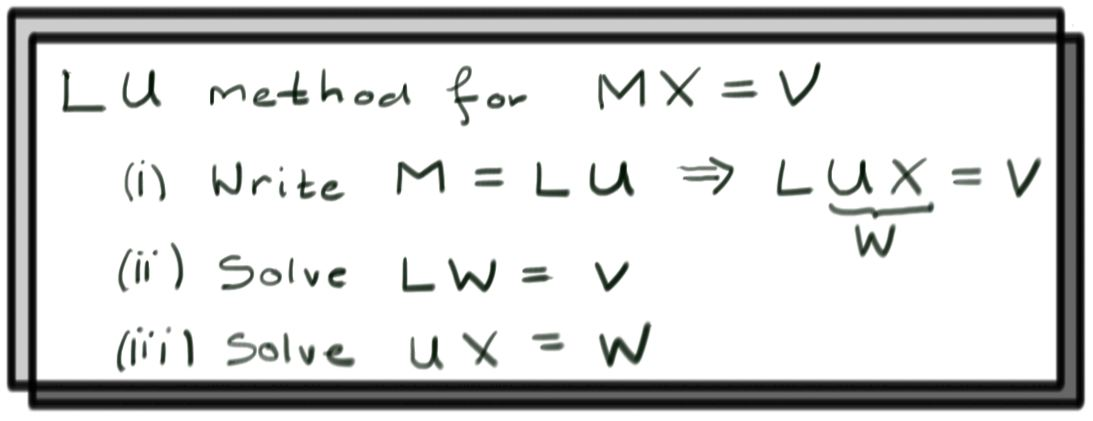
\includegraphics[scale=.3]{\luDecompPath/LU_solution.jpg}
\end{center}
%\end{figure}

\section{Finding an $LU$ Decomposition.}
\label{finding_LU_decomp}
 
For any given matrix, there are actually many different $LU$ decompositions.  However, there is a unique $LU$ decomposition in which the $L$ matrix has ones on the diagonal. In that case $L$ is called a \emph{lower unit triangular matrix}\index{Lower unit triangular matrix}.

To find the $LU$ decomposition, we'll create two sequences of matrices $L_0, L_1, \ldots$ and $U_0, U_1, \ldots$ such that at each step, $L_iU_i=M$.  Each of the $L_i$ will be lower triangular, but only the last $U_i$ will be upper triangular.

Start by setting $L_0=I$ and $U_0=M$, because $L_0U_0=M$. A main concept of this calculation is captured by the following example:

\begin{example}
Consider $$E=\begin{pmatrix}1&0\\\lambda&1\end{pmatrix}\, ,\qquad M=\begin{pmatrix}a&b&c&\cdots\\d&e&f&\cdots\end{pmatrix}\, .$$
Lets compute $EM$
$$
EM=\begin{pmatrix}a&b&c&\cdots\\d+\lambda a&e+\lambda b&f+\lambda c&\cdots\end{pmatrix}\, ,.
$$
Something neat happened here: multiplying $M$ by $E$ performed the row operation $R_2\to R_2+\lambda R-1$ on $M$.
Another interesting fact:
$$
E^{-1}:=\begin{pmatrix}1&0\\-\lambda&1\end{pmatrix}
$$ 
obeys (check this yourself...)
$$
E^{-1} E = 1\, .
$$
Hence $M=E^{-1} E M$ or, writing this out
$$
\begin{pmatrix}a&b&c&\cdots\\d&e&f&\cdots\end{pmatrix}=\begin{pmatrix}1&0\\-\lambda&1\end{pmatrix} \begin{pmatrix}a&b&c&\cdots\\d+\lambda a&e+\lambda b&f+\lambda c&\cdots\end{pmatrix}\, .
$$
Here the matrix on the left is lower triangular, while the matrix on the right has had a row operation performed on it.
\end{example}




\vspace{2mm}
We would like to  use the first row of $U_0$ to zero out the first entry of every row below it.  For our running example, $$U_0=M=\begin{pmatrix}
6 & 18 & 3 \\
2 & 12 & 1 \\
4 & 15 & 3 
\end{pmatrix}\, ,$$ so we would like to perform the row operations $R_2\to R_2 -\frac 13 R_1$ and $R_3\to R_3-\frac 23R_1$.
%so the second row minus $\frac{1}{3}$ of the first row will zero out the first entry in the second row.  Likewise, the third row minus $\frac{2}{3}$ of the first row will zero out the first entry in the third row.
If we perform these row operations on $U_0$ to produce 
$$U_1=\begin{pmatrix}
6 & 18 & 3 \\
0 & 6 & 0 \\
0 & 3 & 1 
\end{pmatrix}\, ,$$
we need to multiply this on the left by a lower triangular matrix $L_1$ so that the product $L_1U_1=M$ still.
The above example shows how to do this:
Set $L_1$ to be the lower triangular matrix whose first column is filled with the minus constants used to zero out the first column of $M$.  Then $$L_1 = \begin{pmatrix}
1 & 0 & 0 \\[1mm]
\frac{1}{3} & 1 & 0 \\[1mm]
\frac{2}{3} & 0 & 1 
\end{pmatrix}\, .$$  
%Set $U_1$ to be the matrix obtained by zeroing out the first column of $M$.  Then $U_1=\begin{pmatrix}
%6 & 18 & 3 \\
%0 & 6 & 0 \\
%0 & 3 & 1 
%\end{pmatrix}$.
By construction $L_1 U_1=M$, but you should compute this yourself as a double check.

Now repeat the process by zeroing the second column of $U_1$ below the diagonal using the second row of $U_1$ using the row operation
$R_3\to R_3-\frac 12 R_2$ to produce
$$U_2=\begin{pmatrix}6&18&3\\0&6&0\\0&0&1\end{pmatrix}\, .$$
The matrix that undoes this row operation is obtained in the same way we found $L_1$ above and is:
$$
\begin{pmatrix}
1&0&0\\
0&1&0\\
0&\frac 12& 0
\end{pmatrix}\, .
$$
Thus our answer for $L_2$ is the product of this matrix with $L_1$, namely
$$
L_2=
\begin{pmatrix}
1 & 0 & 0 \\[1mm]
\frac{1}{3} & 1 & 0 \\[1mm]
\frac{2}{3} & 0 & 1 
\end{pmatrix}\begin{pmatrix}
1&0&0\\
0&1&0\\
0&\frac 12& 0
\end{pmatrix}
=\begin{pmatrix}
1 & 0 & 0 \\[1mm]
\frac{1}{3} & 1 & 0 \\[1mm]
\frac{2}{3} & \frac{1}{2} & 1 
\end{pmatrix}\, .
$$
Notice that it is lower triangular because 

\begin{center}
\textcolor{brown}{THE PRODUCT OF LOWER TRIANGULAR MATRICES IS ALWAYS LOWER TRIANGULAR!}
\end{center}

\noindent
Moreover it is obtained by recording minus the constants used for all our row operations in the appropriate columns (this always works this way).
Moreover, $U_2$ is upper triangular and $M=L_2U_2$, we are done!
Putting this all together we have
$$M=\begin{pmatrix}
6 & 18 & 3 \\
2 & 12 & 1 \\
4 & 15 & 3 
\end{pmatrix}= \begin{pmatrix}
1 & 0 & 0 \\[1mm]
\frac{1}{3} & 1 & 0 \\[1mm]
\frac{2}{3} & \frac{1}{2} & 1 
\end{pmatrix}\begin{pmatrix}
6 & 18 & 3 \\
0 & 6 & 0 \\
0 & 0 & 1 
\end{pmatrix}\, .$$  
%Since $U_2$ is upper-triangular, we're done.  Inserting the new number into $L_1$ to get $L_2$ really is safe: the numbers in the first column don't affect the second column of $U_1$, since the first column of $U_1$ is already zeroed out.

If the matrix you're working with has more than three rows, just continue this process by zeroing out the next column below the diagonal, and repeat until there's nothing left to do.

\videoscriptlink{lu_decomposition_example.mp4}{Another $LU$ decomposition example}{scripts_lu_decomposition_example}

The fractions in the $L$ matrix are admittedly ugly.  For two matrices $LU$, we can multiply one entire column of $L$ by a constant $\lambda$ and divide the corresponding row of $U$ by the same constant without changing the product of the two matrices.  Then:

\begin{eqnarray*}
LU &=& \begin{pmatrix}
1 & 0 & 0 \\[1mm]
\frac{1}{3} & 1 & 0 \\[1mm]
\frac{2}{3} & \frac{1}{2} & 1 
\end{pmatrix}
I
\begin{pmatrix}
6 & 18 & 3 \\
0 & 6 & 0 \\
0 & 0 & 1 
\end{pmatrix} \\
&=&
\begin{pmatrix}
1 & 0 & 0 \\[1mm]
\frac{1}{3} & 1 & 0 \\[1mm]
\frac{2}{3} & \frac{1}{2} & 1 
\end{pmatrix}
\begin{pmatrix}
3 & 0 & 0 \\
0 & 6 & 0 \\
0 & 0 & 1 
\end{pmatrix}
\begin{pmatrix}
\frac{1}{3} & 0 & 0 \\[1mm]
0 & \frac{1}{6} & 0 \\[1mm]
0 & 0 & 1 
\end{pmatrix}
\begin{pmatrix}
6 & 18 & 3 \\
0 & 6 & 0 \\
0 & 0 & 1 
\end{pmatrix} \\
&=&
\begin{pmatrix}
3 & 0 & 0 \\
1 & 6 & 0 \\
2 & 3 & 1 
\end{pmatrix}\begin{pmatrix}
2 & 6 & 1 \\
0 & 1 & 0 \\
0 & 0 & 1 
\end{pmatrix}.
\end{eqnarray*}
The resulting matrix looks nicer, but isn't in standard (lower unit triangular matrix) form.

\reading{11}{2}
%\href{\webworkurl ReadingHomework11/2/}{Reading homework: problem 11.2}

For matrices that are not square, $LU$ decomposition still makes sense.  Given an $m\times n$ matrix $M$, for example we could write $M=LU$ with $L$ a square lower unit triangular matrix, and $U$ a rectangular matrix.  Then $L$ will be an $m\times m$ matrix, and $U$ will be an $m\times n$ matrix (of the same shape as $M$).  From here, the process is exactly the same as for a square matrix.  We create a sequence of matrices $L_i$ and $U_i$ that is eventually the $LU$ decomposition.  Again, we start with $L_0=I$ and $U_0=M$.

\begin{example}
Let's find the $LU$ decomposition of $M=U_0=\begin{pmatrix}
-2 & 1 & 3 \\
-4 & 4 & 1 
\end{pmatrix}$.  Since $M$ is a $2\times 3$ matrix, our decomposition will consist of a $2\times 2$ matrix and a $2\times 3$ matrix.  Then we start with $L_0=I_2=\begin{pmatrix}
1 & 0 \\
0 & 1
\end{pmatrix}$.

The next step is to zero-out the first column of $M$ below the diagonal.  There is only one row to cancel, then, and it can be removed by subtracting $2$ times the first row of $M$ to the second row of $M$.  Then:

\[
L_1=\begin{pmatrix}
1 & 0 \\
2 & 1
\end{pmatrix}, \qquad 
U_1 = \begin{pmatrix}
-2 & 1 & 3 \\
0 & 2 & -5 
\end{pmatrix}
\]
Since $U_1$ is upper triangular, we're done.  With a larger matrix, we would just continue the process.
\end{example}





\section{Block $LDU$ Decomposition}

Let $M$ be a square block matrix with square blocks $X,Y,Z,W$ such that $X^{-1}$ exists.  Then $M$ can be decomposed as a block $LDU$ decomposition, where $D$ is block diagonal, as follows:
\[
M=\begin{pmatrix}
X & Y \\
Z & W
\end{pmatrix}
\]

Then: \[M=\begin{pmatrix}
I &  0 \\
ZX^{-1} & I
\end{pmatrix}\begin{pmatrix}
X & 0 \\
0 & W-ZX^{-1}Y
\end{pmatrix}\begin{pmatrix}
I & X^{-1}Y \\
0 & I
\end{pmatrix}.\]
This can be checked explicitly simply by block-multiplying these three matrices.

\videoscriptlink{lu_decomposition_blocks.mp4}{Block $LDU$ Explanation}{scripts_lu_decomposition_blocks}

\begin{example}
For a $2\times 2$ matrix, we can regard each entry as a block.
\[
\begin{pmatrix}
1 & 2 \\
3 & 4
\end{pmatrix}=
\begin{pmatrix}
1 & 0 \\
3 & 1
\end{pmatrix}
\begin{pmatrix}
1 & 0 \\
0 & -2
\end{pmatrix}
\begin{pmatrix}
1 & 2 \\
0 & 1
\end{pmatrix}
\]
By multiplying the diagonal matrix by the upper triangular matrix, we get the standard $LU$ decomposition of the matrix.
\end{example}


%\section*{References}
%Wikipedia:
%\begin{itemize}
%\item \href{http://en.wikipedia.org/wiki/LU_decomposition}{$LU$ Decomposition}
%\item \href{http://en.wikipedia.org/wiki/Block_LU_decomposition}{Block $LU$ Decomposition}
%\end{itemize}

\section{Review Problems}



\begin{enumerate}

\item Let $D=\begin{pmatrix}
\lambda_1 & \mc0 \\
\mc0 & \lambda_2 \\
\end{pmatrix}$.
\begin{enumerate}
\item Write $D$ in terms of the vectors $e_1$ and $e_2$, and their transposes.
\item Suppose $P=\begin{pmatrix}
a & b \\
c & d \\
\end{pmatrix}$ is invertible.  Show that $D$ is similar to
\[
M=\frac{1}{ad-bc}\begin{pmatrix}
\lambda_1ad-\lambda_2bc & -(\lambda_1-\lambda_2)ab \\[1mm]
(\lambda_1-\lambda_2)cd & -\lambda_1bc + \lambda_2ad
\end{pmatrix}.
\]
\item Suppose the vectors $\rowvec{a,b}$ and $\rowvec{c,d}$ are orthogonal.  What can you say about $M$ in this case? (Hint: think about what \(M^T\) is equal to.)
\end{enumerate}

\phantomnewpage

\item \label{orthogprob} Suppose $S=\{v_1, \ldots, v_n \}$ is an \emph{orthogonal} (not orthonormal) basis for~$\Re^n$.  Then we can write any vector $v$ as $v=\sum_ic^iv_i$ for some constants $c^i$.  Find a formula for the constants $c^i$ in terms of $v$ and the vectors in~$S$.

\Videoscriptlink{orthonormal_bases_hint.mp4}{Hint}{scripts_orthonormal_bases_hint}
\phantomnewpage

\item \label{orthogprojprob} Let $u,v$ be linearly independent vectors in $\Re^3$, and $P=\spa \{ u,v\}$ be the plane spanned by $u$ and $v$.  
\begin{enumerate}
\item Is the vector $v^\bot := v-\frac{u\cdot v}{u\cdot u}u$ in the plane $P$?
\item  What is the (cosine of the) angle between $v^\bot$ and $u$?
\item %Given your solution to the above, 
How can you find a third vector perpendicular to both $u$ and $v^\bot$?
\item  Construct an orthonormal basis for $\Re^3$ from $u$ and $v$.
\item  Test your abstract formul\ae\ starting with 
\[
u=\rowvec{1 , 2 , 0} \text{ and } v=\rowvec{0 , 1 , 1}.
\]
\end{enumerate}

\Videoscriptlink{orthonormal_bases_hint3.mp4}{Hint}{scripts_orthonormal_bases_hint3}

\phantomnewpage



\item Find an orthonormal  basis for $\Re^4$ which includes $(1,1,1,1)$ using the following procedure:\\
\begin{enumerate} 
\item Pick a vector perpendicular to the vector 
$$v_1 =\colvec{1\\1\\1\\1}$$ from the solution set of the matrix equation $$v_1^Tx=0\, .$$ Pick the vector $v_2$ obtained from the standard Gaussian elimination procedure which is the coefficient of $x_2$.
\item Pick a vector perpendicular to both $v_1$ and $v_2$ from the solutions set of the matrix equation $$\colvec{v_1^T\\[1mm]v_2^T}x=0\, .$$ Pick the vector $v_3$ obtained from the standard Gaussian elimination procedure with $x_3$ as the coefficient. 
\item Pick a vector perpendicular to $v_1,v_2,$ and $v_3$ from the solution set of the matrix equation $$\colvec{v_1^T\\[1mm]v_2^T\\[1mm]v_3^T}x=0\, .$$  Pick the vector $v_4$ obtained from the standard Gaussian elimination procedure with $x_3$ as the coefficient. 
\item Normalize the four vectors obtained   above.
\end{enumerate}


\item Use the inner product $$f\cdot g := \int_0^1 f(x)g(x)dx$$  on the vector space $V={\rm span} \{1,x,x^2,x^3\}$ to perform the Gram-Schmidt procedure on the set of vectors $\{1,x,x^2,x^3\}$. 

\item Use the inner product $$f\cdot g := \int_0^{2\pi} f(x)g(x)dx$$  on the vector space $V={\rm span} \{\sin(x),\sin(2x),\sin(3x) \}$ to perform the Gram-Schmidt procedure on the set of vectors $\{\sin(x),\sin(2x),\sin(3x) \}$. \\
Try to build an orthonormal basis for the vector space $$\spa \{ \sin(nx)~| ~n\in \N \}\, .$$
%What do you suspect about the vector space $\spa \{ \sin(nx)~| ~n\in \N \}$?\\
%What do you suspect about the vector space $\spa \{ \sin(ax)~|~ a \in \Re \}$?
\item 
\begin{enumerate}
\item
Show that if $Q$ is an orthogonal $n\times n$ matrix, then $$u\dotprod v = (Qu)\dotprod (Qv)\, ,$$ for any $u,v\in \Re^n$. That is, $Q$ preserves the inner product. 
\item Does $Q$ preserve the outer product? 
\item  If the set of vectors $\{ u_1,\dots,u_n\}$ is orthonormal and $\{ \lambda_1,\cdots,\lambda_n\}$ is a set of numbers, 
then what are the eigenvalues and eigenvectors of the matrix
$M=\sum_{i=1}^n \lambda_i u_i u_i^T$? 
\item How would the eigenvectors and eigenvalues of this matrix change if we replaced  $\{ u_1,\dots,u_n\}$ by $\{ Qu_1,\dots,Q u_n\}$?
\end{enumerate}


\item Carefully write out the Gram-Schmidt procedure for the set of vectors 
$$\left\{ \colvec{1\\1\\1}, \colvec{1\\-1\\1}, \colvec{1\\1\\-1} \right\} \, .$$ Is it possible to rescale the second vector obtained in the procedure to a vector with integer components? 


\item 
\label{basisortho}
\begin{enumerate}
\item Suppose $u$ and $v$ are linearly independent.  Show that $u$ and $v^\perp$ are also linearly independent.  Explain why $\{u, v^\perp\}$ is a basis for $\spa \{u,v\}$.



\Videoscriptlink{gram_schmidt_and_orthogonal_complements_hint.mp4}{Hint}{gram_schmidt_and_orthogonal_complements_hint}

\item Repeat the previous problem, but with three independent vectors $u,v,w$
 where $v^\perp$ and $w^\perp$ are as defined by the Gram-Schmidt procedure. 
\end{enumerate}

\phantomnewpage


\item \label{QRprob} Find the $QR$ factorization of
$$
M=\begin{pmatrix}1&0&\phantom{\!-}2\\-1&2&0\\-1&-2&2
\end{pmatrix}\, .
$$

\phantomnewpage

\item Given any three vectors $u,v,w$, when do $v^\perp$ or $w^\perp$ of the Gram--Schmidt procedure vanish?

\phantomnewpage

\item For $U$ a subspace of $W$, use the subspace theorem to check that $U^\perp$ is a subspace of $W$.

\phantomnewpage


\phantomnewpage

\item %(Extra Credit) 
Let $S_n$ and $A_n$ define the space of $n \times n$ symmetric and anti-symmetric matrices, respectively. These are subspaces of the vector space $M^n_n$ of all $n\times n$ matrices. What is $\dim M^n_n$, $\dim S_n$, and $\dim A_n$? Show that $M^n_n = S_n + A_n$. Define an inner product on square matrices
$$
M\cdot N ={\rm tr} MN\, .
$$
Is $A_n^{\perp}=S_n$? Is $M^n_n = S_n \oplus A_n$?

%\emph{Hint: Note that $\dim S_n = \dim U_n$ where $U_n$ is the vector space of all $n \times n$ upper triangular matrices, and also note that $\dim A_n = \dim \widetilde{U}_n$ where $\widetilde{U}_n$ is the vector space of all strictly $n \times n$ upper triangular matrices (\emph{i.e.} the diagonal entries are all 0).}

\item The vector space $V={\rm span} \{ \sin(t),\sin(2t), \sin(3t) , \sin(3t)\}$ has an inner product: 
$$f\cdot g:=\int _0^{2\pi}f(t)g(t) dt\, .$$ Find the orthogonal compliment to $U={\rm span} \{ \sin(t)+\sin(2t) \}$ in $V$. Express $\sin(t)-\sin(2t)$ as  the sum of vectors from $U$ and $U^\perp$.

\end{enumerate}

\phantomnewpage

\newpage


%\chapter{\luDecompTitle}
\label{LUdecomp}

Certain matrices are easier to work with than others.  In this section, we will see how to write any square\footnote{The case where $M$ is not square is dealt with at the end of the lecture.} matrix $M$ as the product of two simpler matrices.  We will write $$M=LU\, ,$$ where:
\begin{itemize}
\item $L$ is \emph{lower triangular}\index{Lower triangular matrix}.  This means that all entries above the main diagonal are zero.  In notation,
$L=(l^i_j)$ with $l^i_j=0$ for all $j>i$.
\[L=\begin{pmatrix}
l^1_1 & 0 & 0 & \cdots \\
l^2_1 & l^2_2 & 0 & \cdots \\
l^3_1 & l^3_2 & l^3_3 & \cdots \\
\vdots & \vdots & \vdots & \ddots \\
\end{pmatrix}
\]

\item $U$ is \emph{upper triangular}\index{Upper triangular matrix}.  This means that all entries below the main diagonal are zero.  In notation,
$U=(u^i_j)$ with $u^i_j=0$ for all $j<i$.
\[U=\begin{pmatrix}
u^1_1 & u^1_2 & u^1_3 & \cdots \\
0 & u^2_2 & u^2_3 & \cdots \\
0 & 0 & u^3_3 & \cdots \\
\vdots & \vdots & \vdots & \ddots \\
\end{pmatrix}
\]
\end{itemize}
$M=LU$ is called an \emph{$LU$ decomposition}\index{LU@$LU$ decomposition} of $M$.

This is a useful trick for  computational reasons; it is much easier to compute the inverse of an upper or lower triangular matrix than general matrices.  Since inverses are useful for solving linear systems, this makes solving any linear system associated to the matrix much faster as well.  The determinant---a very important quantity associated with any square matrix---is very easy to compute for triangular matrices.

\begin{example}
Linear systems associated to upper triangular matrices are very easy to solve by back substitution.
\[
\begin{amatrix}{2}
a & b & 1 \\
0 & c & e \\
\end{amatrix} \ \Rightarrow \ y=\frac{e}{c}\, , \quad x=\frac{1}{a}\left(1-\frac{be}{c}\right)
\]

\[
\begin{amatrix}{3}
1 & 0 & 0 & d \\
a & 1 & 0 & e \\
b & c & 1 & f \\
\end{amatrix} \Rightarrow x=d\, , \qquad y=e-ad\, , \qquad z=f-bd-c(e-ad)
\]
For lower triangular matrices, \emph{back} substitution\index{Back substitution} gives a quick solution; for upper triangular matrices, \emph{forward} substitution\index{Forward substitution} gives the solution.
\end{example}





\section{Using $LU$ Decomposition to Solve Linear Systems}

Suppose we have $M=LU$ and want to solve the system
\[
MX=LUX=V.
\]

\begin{itemize}
\item{Step 1:} Set $W=\colvec{u\\v\\w}=UX$.  

\item{Step 2:} Solve the system $LW=V$.  This should be simple by forward substitution since $L$ is lower triangular.  Suppose the solution to $LW=V$ is $W_0$.  

\item{Step 3:} Now solve the system $UX=W_0$.  This should be easy by backward substitution, since $U$ is upper triangular.  The solution to this system is the solution to the original system.
\end{itemize}
We can think of this as using the matrix $L$ to perform row operations on the matrix $U$ in order to solve the system; this idea also appears in the  study of determinants.

%\href{\webworkurl ReadingHomework11/1/}{Reading homework: problem 11.1}
\reading{11}{1}

\begin{example}
Consider the linear system:
\[
      \begin{linsys}{4}
            6x & +&18y & +&3z         &=& 3  \\[1mm]
            2x & +&12y & +&z	    &=& 19 \\[1mm]
            4x & +&15y & +&3z         &=& 0  
      \end{linsys}
\]

An $LU$ decomposition for the associated matrix $M$ is:
\[
\begin{pmatrix}
6 & 18 & 3 \\
2 & 12 & 1 \\
4 & 15 & 3 
\end{pmatrix} =
\begin{pmatrix}
3 & 0 & 0 \\
1 & 6 & 0 \\
2 & 3 & 1 
\end{pmatrix}
\begin{pmatrix}
2 & 6 & 1 \\
0 & 1 & 0 \\
0 & 0 & 1 
\end{pmatrix}.
\]

\begin{itemize}
\item{Step 1:} \hypertarget{LUproc}{Set} $W=\colvec{u\\v\\w}=UX$.  

\item{Step 2:} Solve the system $LW=V$:

\[
\begin{pmatrix}
3 & 0 & 0 \\
1 & 6 & 0 \\
2 & 3 & 1 
\end{pmatrix}
\colvec{u\\v\\w} =
\colvec{3\\19\\0}
\]

By substitution, we get $u=1$, $v=3$, and $w=-11$.  Then 
\[W_0=\colvec{1\\3\\-11}\]

\item{Step 3:} Solve the system $UX=W_0$.  
\[
\begin{pmatrix}
2 & 6 & 1 \\
0 & 1 & 0 \\
0 & 0 & 1 
\end{pmatrix}
\colvec{x\\y\\z} =
\colvec{1\\3\\-11}
\]
Back substitution gives $z=-11, y=3$, and $x=-3$.  

Then $X=\colvec{-3\\3\\-11}$, and we're done.
\end{itemize}
\end{example}

\videoscriptlink{lu_decomposition_using_lu_decomp.mp4}{Using a $LU$ decomposition}{scripts_lu_decomposition_using_lu_example}

%\begin{figure}
\begin{center}
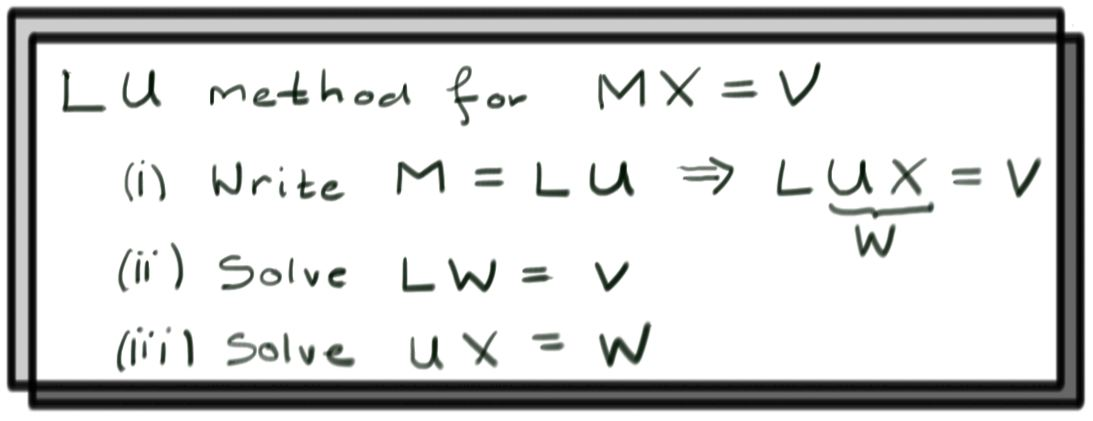
\includegraphics[scale=.3]{\luDecompPath/LU_solution.jpg}
\end{center}
%\end{figure}

\section{Finding an $LU$ Decomposition.}
\label{finding_LU_decomp}
 
For any given matrix, there are actually many different $LU$ decompositions.  However, there is a unique $LU$ decomposition in which the $L$ matrix has ones on the diagonal. In that case $L$ is called a \emph{lower unit triangular matrix}\index{Lower unit triangular matrix}.

To find the $LU$ decomposition, we'll create two sequences of matrices $L_0, L_1, \ldots$ and $U_0, U_1, \ldots$ such that at each step, $L_iU_i=M$.  Each of the $L_i$ will be lower triangular, but only the last $U_i$ will be upper triangular.

Start by setting $L_0=I$ and $U_0=M$, because $L_0U_0=M$. A main concept of this calculation is captured by the following example:

\begin{example}
Consider $$E=\begin{pmatrix}1&0\\\lambda&1\end{pmatrix}\, ,\qquad M=\begin{pmatrix}a&b&c&\cdots\\d&e&f&\cdots\end{pmatrix}\, .$$
Lets compute $EM$
$$
EM=\begin{pmatrix}a&b&c&\cdots\\d+\lambda a&e+\lambda b&f+\lambda c&\cdots\end{pmatrix}\, ,.
$$
Something neat happened here: multiplying $M$ by $E$ performed the row operation $R_2\to R_2+\lambda R-1$ on $M$.
Another interesting fact:
$$
E^{-1}:=\begin{pmatrix}1&0\\-\lambda&1\end{pmatrix}
$$ 
obeys (check this yourself...)
$$
E^{-1} E = 1\, .
$$
Hence $M=E^{-1} E M$ or, writing this out
$$
\begin{pmatrix}a&b&c&\cdots\\d&e&f&\cdots\end{pmatrix}=\begin{pmatrix}1&0\\-\lambda&1\end{pmatrix} \begin{pmatrix}a&b&c&\cdots\\d+\lambda a&e+\lambda b&f+\lambda c&\cdots\end{pmatrix}\, .
$$
Here the matrix on the left is lower triangular, while the matrix on the right has had a row operation performed on it.
\end{example}




\vspace{2mm}
We would like to  use the first row of $U_0$ to zero out the first entry of every row below it.  For our running example, $$U_0=M=\begin{pmatrix}
6 & 18 & 3 \\
2 & 12 & 1 \\
4 & 15 & 3 
\end{pmatrix}\, ,$$ so we would like to perform the row operations $R_2\to R_2 -\frac 13 R_1$ and $R_3\to R_3-\frac 23R_1$.
%so the second row minus $\frac{1}{3}$ of the first row will zero out the first entry in the second row.  Likewise, the third row minus $\frac{2}{3}$ of the first row will zero out the first entry in the third row.
If we perform these row operations on $U_0$ to produce 
$$U_1=\begin{pmatrix}
6 & 18 & 3 \\
0 & 6 & 0 \\
0 & 3 & 1 
\end{pmatrix}\, ,$$
we need to multiply this on the left by a lower triangular matrix $L_1$ so that the product $L_1U_1=M$ still.
The above example shows how to do this:
Set $L_1$ to be the lower triangular matrix whose first column is filled with the minus constants used to zero out the first column of $M$.  Then $$L_1 = \begin{pmatrix}
1 & 0 & 0 \\[1mm]
\frac{1}{3} & 1 & 0 \\[1mm]
\frac{2}{3} & 0 & 1 
\end{pmatrix}\, .$$  
%Set $U_1$ to be the matrix obtained by zeroing out the first column of $M$.  Then $U_1=\begin{pmatrix}
%6 & 18 & 3 \\
%0 & 6 & 0 \\
%0 & 3 & 1 
%\end{pmatrix}$.
By construction $L_1 U_1=M$, but you should compute this yourself as a double check.

Now repeat the process by zeroing the second column of $U_1$ below the diagonal using the second row of $U_1$ using the row operation
$R_3\to R_3-\frac 12 R_2$ to produce
$$U_2=\begin{pmatrix}6&18&3\\0&6&0\\0&0&1\end{pmatrix}\, .$$
The matrix that undoes this row operation is obtained in the same way we found $L_1$ above and is:
$$
\begin{pmatrix}
1&0&0\\
0&1&0\\
0&\frac 12& 0
\end{pmatrix}\, .
$$
Thus our answer for $L_2$ is the product of this matrix with $L_1$, namely
$$
L_2=
\begin{pmatrix}
1 & 0 & 0 \\[1mm]
\frac{1}{3} & 1 & 0 \\[1mm]
\frac{2}{3} & 0 & 1 
\end{pmatrix}\begin{pmatrix}
1&0&0\\
0&1&0\\
0&\frac 12& 0
\end{pmatrix}
=\begin{pmatrix}
1 & 0 & 0 \\[1mm]
\frac{1}{3} & 1 & 0 \\[1mm]
\frac{2}{3} & \frac{1}{2} & 1 
\end{pmatrix}\, .
$$
Notice that it is lower triangular because 

\begin{center}
\textcolor{brown}{THE PRODUCT OF LOWER TRIANGULAR MATRICES IS ALWAYS LOWER TRIANGULAR!}
\end{center}

\noindent
Moreover it is obtained by recording minus the constants used for all our row operations in the appropriate columns (this always works this way).
Moreover, $U_2$ is upper triangular and $M=L_2U_2$, we are done!
Putting this all together we have
$$M=\begin{pmatrix}
6 & 18 & 3 \\
2 & 12 & 1 \\
4 & 15 & 3 
\end{pmatrix}= \begin{pmatrix}
1 & 0 & 0 \\[1mm]
\frac{1}{3} & 1 & 0 \\[1mm]
\frac{2}{3} & \frac{1}{2} & 1 
\end{pmatrix}\begin{pmatrix}
6 & 18 & 3 \\
0 & 6 & 0 \\
0 & 0 & 1 
\end{pmatrix}\, .$$  
%Since $U_2$ is upper-triangular, we're done.  Inserting the new number into $L_1$ to get $L_2$ really is safe: the numbers in the first column don't affect the second column of $U_1$, since the first column of $U_1$ is already zeroed out.

If the matrix you're working with has more than three rows, just continue this process by zeroing out the next column below the diagonal, and repeat until there's nothing left to do.

\videoscriptlink{lu_decomposition_example.mp4}{Another $LU$ decomposition example}{scripts_lu_decomposition_example}

The fractions in the $L$ matrix are admittedly ugly.  For two matrices $LU$, we can multiply one entire column of $L$ by a constant $\lambda$ and divide the corresponding row of $U$ by the same constant without changing the product of the two matrices.  Then:

\begin{eqnarray*}
LU &=& \begin{pmatrix}
1 & 0 & 0 \\[1mm]
\frac{1}{3} & 1 & 0 \\[1mm]
\frac{2}{3} & \frac{1}{2} & 1 
\end{pmatrix}
I
\begin{pmatrix}
6 & 18 & 3 \\
0 & 6 & 0 \\
0 & 0 & 1 
\end{pmatrix} \\
&=&
\begin{pmatrix}
1 & 0 & 0 \\[1mm]
\frac{1}{3} & 1 & 0 \\[1mm]
\frac{2}{3} & \frac{1}{2} & 1 
\end{pmatrix}
\begin{pmatrix}
3 & 0 & 0 \\
0 & 6 & 0 \\
0 & 0 & 1 
\end{pmatrix}
\begin{pmatrix}
\frac{1}{3} & 0 & 0 \\[1mm]
0 & \frac{1}{6} & 0 \\[1mm]
0 & 0 & 1 
\end{pmatrix}
\begin{pmatrix}
6 & 18 & 3 \\
0 & 6 & 0 \\
0 & 0 & 1 
\end{pmatrix} \\
&=&
\begin{pmatrix}
3 & 0 & 0 \\
1 & 6 & 0 \\
2 & 3 & 1 
\end{pmatrix}\begin{pmatrix}
2 & 6 & 1 \\
0 & 1 & 0 \\
0 & 0 & 1 
\end{pmatrix}.
\end{eqnarray*}
The resulting matrix looks nicer, but isn't in standard (lower unit triangular matrix) form.

\reading{11}{2}
%\href{\webworkurl ReadingHomework11/2/}{Reading homework: problem 11.2}

For matrices that are not square, $LU$ decomposition still makes sense.  Given an $m\times n$ matrix $M$, for example we could write $M=LU$ with $L$ a square lower unit triangular matrix, and $U$ a rectangular matrix.  Then $L$ will be an $m\times m$ matrix, and $U$ will be an $m\times n$ matrix (of the same shape as $M$).  From here, the process is exactly the same as for a square matrix.  We create a sequence of matrices $L_i$ and $U_i$ that is eventually the $LU$ decomposition.  Again, we start with $L_0=I$ and $U_0=M$.

\begin{example}
Let's find the $LU$ decomposition of $M=U_0=\begin{pmatrix}
-2 & 1 & 3 \\
-4 & 4 & 1 
\end{pmatrix}$.  Since $M$ is a $2\times 3$ matrix, our decomposition will consist of a $2\times 2$ matrix and a $2\times 3$ matrix.  Then we start with $L_0=I_2=\begin{pmatrix}
1 & 0 \\
0 & 1
\end{pmatrix}$.

The next step is to zero-out the first column of $M$ below the diagonal.  There is only one row to cancel, then, and it can be removed by subtracting $2$ times the first row of $M$ to the second row of $M$.  Then:

\[
L_1=\begin{pmatrix}
1 & 0 \\
2 & 1
\end{pmatrix}, \qquad 
U_1 = \begin{pmatrix}
-2 & 1 & 3 \\
0 & 2 & -5 
\end{pmatrix}
\]
Since $U_1$ is upper triangular, we're done.  With a larger matrix, we would just continue the process.
\end{example}





\section{Block $LDU$ Decomposition}

Let $M$ be a square block matrix with square blocks $X,Y,Z,W$ such that $X^{-1}$ exists.  Then $M$ can be decomposed as a block $LDU$ decomposition, where $D$ is block diagonal, as follows:
\[
M=\begin{pmatrix}
X & Y \\
Z & W
\end{pmatrix}
\]

Then: \[M=\begin{pmatrix}
I &  0 \\
ZX^{-1} & I
\end{pmatrix}\begin{pmatrix}
X & 0 \\
0 & W-ZX^{-1}Y
\end{pmatrix}\begin{pmatrix}
I & X^{-1}Y \\
0 & I
\end{pmatrix}.\]
This can be checked explicitly simply by block-multiplying these three matrices.

\videoscriptlink{lu_decomposition_blocks.mp4}{Block $LDU$ Explanation}{scripts_lu_decomposition_blocks}

\begin{example}
For a $2\times 2$ matrix, we can regard each entry as a block.
\[
\begin{pmatrix}
1 & 2 \\
3 & 4
\end{pmatrix}=
\begin{pmatrix}
1 & 0 \\
3 & 1
\end{pmatrix}
\begin{pmatrix}
1 & 0 \\
0 & -2
\end{pmatrix}
\begin{pmatrix}
1 & 2 \\
0 & 1
\end{pmatrix}
\]
By multiplying the diagonal matrix by the upper triangular matrix, we get the standard $LU$ decomposition of the matrix.
\end{example}


%\section*{References}
%Wikipedia:
%\begin{itemize}
%\item \href{http://en.wikipedia.org/wiki/LU_decomposition}{$LU$ Decomposition}
%\item \href{http://en.wikipedia.org/wiki/Block_LU_decomposition}{Block $LU$ Decomposition}
%\end{itemize}

\section{Review Problems}



\begin{enumerate}

\item Let $D=\begin{pmatrix}
\lambda_1 & \mc0 \\
\mc0 & \lambda_2 \\
\end{pmatrix}$.
\begin{enumerate}
\item Write $D$ in terms of the vectors $e_1$ and $e_2$, and their transposes.
\item Suppose $P=\begin{pmatrix}
a & b \\
c & d \\
\end{pmatrix}$ is invertible.  Show that $D$ is similar to
\[
M=\frac{1}{ad-bc}\begin{pmatrix}
\lambda_1ad-\lambda_2bc & -(\lambda_1-\lambda_2)ab \\[1mm]
(\lambda_1-\lambda_2)cd & -\lambda_1bc + \lambda_2ad
\end{pmatrix}.
\]
\item Suppose the vectors $\rowvec{a,b}$ and $\rowvec{c,d}$ are orthogonal.  What can you say about $M$ in this case? (Hint: think about what \(M^T\) is equal to.)
\end{enumerate}

\phantomnewpage

\item \label{orthogprob} Suppose $S=\{v_1, \ldots, v_n \}$ is an \emph{orthogonal} (not orthonormal) basis for~$\Re^n$.  Then we can write any vector $v$ as $v=\sum_ic^iv_i$ for some constants $c^i$.  Find a formula for the constants $c^i$ in terms of $v$ and the vectors in~$S$.

\Videoscriptlink{orthonormal_bases_hint.mp4}{Hint}{scripts_orthonormal_bases_hint}
\phantomnewpage

\item \label{orthogprojprob} Let $u,v$ be linearly independent vectors in $\Re^3$, and $P=\spa \{ u,v\}$ be the plane spanned by $u$ and $v$.  
\begin{enumerate}
\item Is the vector $v^\bot := v-\frac{u\cdot v}{u\cdot u}u$ in the plane $P$?
\item  What is the (cosine of the) angle between $v^\bot$ and $u$?
\item %Given your solution to the above, 
How can you find a third vector perpendicular to both $u$ and $v^\bot$?
\item  Construct an orthonormal basis for $\Re^3$ from $u$ and $v$.
\item  Test your abstract formul\ae\ starting with 
\[
u=\rowvec{1 , 2 , 0} \text{ and } v=\rowvec{0 , 1 , 1}.
\]
\end{enumerate}

\Videoscriptlink{orthonormal_bases_hint3.mp4}{Hint}{scripts_orthonormal_bases_hint3}

\phantomnewpage



\item Find an orthonormal  basis for $\Re^4$ which includes $(1,1,1,1)$ using the following procedure:\\
\begin{enumerate} 
\item Pick a vector perpendicular to the vector 
$$v_1 =\colvec{1\\1\\1\\1}$$ from the solution set of the matrix equation $$v_1^Tx=0\, .$$ Pick the vector $v_2$ obtained from the standard Gaussian elimination procedure which is the coefficient of $x_2$.
\item Pick a vector perpendicular to both $v_1$ and $v_2$ from the solutions set of the matrix equation $$\colvec{v_1^T\\[1mm]v_2^T}x=0\, .$$ Pick the vector $v_3$ obtained from the standard Gaussian elimination procedure with $x_3$ as the coefficient. 
\item Pick a vector perpendicular to $v_1,v_2,$ and $v_3$ from the solution set of the matrix equation $$\colvec{v_1^T\\[1mm]v_2^T\\[1mm]v_3^T}x=0\, .$$  Pick the vector $v_4$ obtained from the standard Gaussian elimination procedure with $x_3$ as the coefficient. 
\item Normalize the four vectors obtained   above.
\end{enumerate}


\item Use the inner product $$f\cdot g := \int_0^1 f(x)g(x)dx$$  on the vector space $V={\rm span} \{1,x,x^2,x^3\}$ to perform the Gram-Schmidt procedure on the set of vectors $\{1,x,x^2,x^3\}$. 

\item Use the inner product $$f\cdot g := \int_0^{2\pi} f(x)g(x)dx$$  on the vector space $V={\rm span} \{\sin(x),\sin(2x),\sin(3x) \}$ to perform the Gram-Schmidt procedure on the set of vectors $\{\sin(x),\sin(2x),\sin(3x) \}$. \\
Try to build an orthonormal basis for the vector space $$\spa \{ \sin(nx)~| ~n\in \N \}\, .$$
%What do you suspect about the vector space $\spa \{ \sin(nx)~| ~n\in \N \}$?\\
%What do you suspect about the vector space $\spa \{ \sin(ax)~|~ a \in \Re \}$?
\item 
\begin{enumerate}
\item
Show that if $Q$ is an orthogonal $n\times n$ matrix, then $$u\dotprod v = (Qu)\dotprod (Qv)\, ,$$ for any $u,v\in \Re^n$. That is, $Q$ preserves the inner product. 
\item Does $Q$ preserve the outer product? 
\item  If the set of vectors $\{ u_1,\dots,u_n\}$ is orthonormal and $\{ \lambda_1,\cdots,\lambda_n\}$ is a set of numbers, 
then what are the eigenvalues and eigenvectors of the matrix
$M=\sum_{i=1}^n \lambda_i u_i u_i^T$? 
\item How would the eigenvectors and eigenvalues of this matrix change if we replaced  $\{ u_1,\dots,u_n\}$ by $\{ Qu_1,\dots,Q u_n\}$?
\end{enumerate}


\item Carefully write out the Gram-Schmidt procedure for the set of vectors 
$$\left\{ \colvec{1\\1\\1}, \colvec{1\\-1\\1}, \colvec{1\\1\\-1} \right\} \, .$$ Is it possible to rescale the second vector obtained in the procedure to a vector with integer components? 


\item 
\label{basisortho}
\begin{enumerate}
\item Suppose $u$ and $v$ are linearly independent.  Show that $u$ and $v^\perp$ are also linearly independent.  Explain why $\{u, v^\perp\}$ is a basis for $\spa \{u,v\}$.



\Videoscriptlink{gram_schmidt_and_orthogonal_complements_hint.mp4}{Hint}{gram_schmidt_and_orthogonal_complements_hint}

\item Repeat the previous problem, but with three independent vectors $u,v,w$
 where $v^\perp$ and $w^\perp$ are as defined by the Gram-Schmidt procedure. 
\end{enumerate}

\phantomnewpage


\item \label{QRprob} Find the $QR$ factorization of
$$
M=\begin{pmatrix}1&0&\phantom{\!-}2\\-1&2&0\\-1&-2&2
\end{pmatrix}\, .
$$

\phantomnewpage

\item Given any three vectors $u,v,w$, when do $v^\perp$ or $w^\perp$ of the Gram--Schmidt procedure vanish?

\phantomnewpage

\item For $U$ a subspace of $W$, use the subspace theorem to check that $U^\perp$ is a subspace of $W$.

\phantomnewpage


\phantomnewpage

\item %(Extra Credit) 
Let $S_n$ and $A_n$ define the space of $n \times n$ symmetric and anti-symmetric matrices, respectively. These are subspaces of the vector space $M^n_n$ of all $n\times n$ matrices. What is $\dim M^n_n$, $\dim S_n$, and $\dim A_n$? Show that $M^n_n = S_n + A_n$. Define an inner product on square matrices
$$
M\cdot N ={\rm tr} MN\, .
$$
Is $A_n^{\perp}=S_n$? Is $M^n_n = S_n \oplus A_n$?

%\emph{Hint: Note that $\dim S_n = \dim U_n$ where $U_n$ is the vector space of all $n \times n$ upper triangular matrices, and also note that $\dim A_n = \dim \widetilde{U}_n$ where $\widetilde{U}_n$ is the vector space of all strictly $n \times n$ upper triangular matrices (\emph{i.e.} the diagonal entries are all 0).}

\item The vector space $V={\rm span} \{ \sin(t),\sin(2t), \sin(3t) , \sin(3t)\}$ has an inner product: 
$$f\cdot g:=\int _0^{2\pi}f(t)g(t) dt\, .$$ Find the orthogonal compliment to $U={\rm span} \{ \sin(t)+\sin(2t) \}$ in $V$. Express $\sin(t)-\sin(2t)$ as  the sum of vectors from $U$ and $U^\perp$.

\end{enumerate}

\phantomnewpage

\newpage


\chapter{\luDecompTitle}
\label{LUdecomp}

Certain matrices are easier to work with than others.  In this section, we will see how to write any square\footnote{The case where $M$ is not square is dealt with at the end of the lecture.} matrix $M$ as the product of two simpler matrices.  We will write $$M=LU\, ,$$ where:
\begin{itemize}
\item $L$ is \emph{lower triangular}\index{Lower triangular matrix}.  This means that all entries above the main diagonal are zero.  In notation,
$L=(l^i_j)$ with $l^i_j=0$ for all $j>i$.
\[L=\begin{pmatrix}
l^1_1 & 0 & 0 & \cdots \\
l^2_1 & l^2_2 & 0 & \cdots \\
l^3_1 & l^3_2 & l^3_3 & \cdots \\
\vdots & \vdots & \vdots & \ddots \\
\end{pmatrix}
\]

\item $U$ is \emph{upper triangular}\index{Upper triangular matrix}.  This means that all entries below the main diagonal are zero.  In notation,
$U=(u^i_j)$ with $u^i_j=0$ for all $j<i$.
\[U=\begin{pmatrix}
u^1_1 & u^1_2 & u^1_3 & \cdots \\
0 & u^2_2 & u^2_3 & \cdots \\
0 & 0 & u^3_3 & \cdots \\
\vdots & \vdots & \vdots & \ddots \\
\end{pmatrix}
\]
\end{itemize}
$M=LU$ is called an \emph{$LU$ decomposition}\index{LU@$LU$ decomposition} of $M$.

This is a useful trick for  computational reasons; it is much easier to compute the inverse of an upper or lower triangular matrix than general matrices.  Since inverses are useful for solving linear systems, this makes solving any linear system associated to the matrix much faster as well.  The determinant---a very important quantity associated with any square matrix---is very easy to compute for triangular matrices.

\begin{example}
Linear systems associated to upper triangular matrices are very easy to solve by back substitution.
\[
\begin{amatrix}{2}
a & b & 1 \\
0 & c & e \\
\end{amatrix} \ \Rightarrow \ y=\frac{e}{c}\, , \quad x=\frac{1}{a}\left(1-\frac{be}{c}\right)
\]

\[
\begin{amatrix}{3}
1 & 0 & 0 & d \\
a & 1 & 0 & e \\
b & c & 1 & f \\
\end{amatrix} \Rightarrow x=d\, , \qquad y=e-ad\, , \qquad z=f-bd-c(e-ad)
\]
For lower triangular matrices, \emph{back} substitution\index{Back substitution} gives a quick solution; for upper triangular matrices, \emph{forward} substitution\index{Forward substitution} gives the solution.
\end{example}





\section{Using $LU$ Decomposition to Solve Linear Systems}

Suppose we have $M=LU$ and want to solve the system
\[
MX=LUX=V.
\]

\begin{itemize}
\item{Step 1:} Set $W=\colvec{u\\v\\w}=UX$.  

\item{Step 2:} Solve the system $LW=V$.  This should be simple by forward substitution since $L$ is lower triangular.  Suppose the solution to $LW=V$ is $W_0$.  

\item{Step 3:} Now solve the system $UX=W_0$.  This should be easy by backward substitution, since $U$ is upper triangular.  The solution to this system is the solution to the original system.
\end{itemize}
We can think of this as using the matrix $L$ to perform row operations on the matrix $U$ in order to solve the system; this idea also appears in the  study of determinants.

%\href{\webworkurl ReadingHomework11/1/}{Reading homework: problem 11.1}
\reading{11}{1}

\begin{example}
Consider the linear system:
\[
      \begin{linsys}{4}
            6x & +&18y & +&3z         &=& 3  \\[1mm]
            2x & +&12y & +&z	    &=& 19 \\[1mm]
            4x & +&15y & +&3z         &=& 0  
      \end{linsys}
\]

An $LU$ decomposition for the associated matrix $M$ is:
\[
\begin{pmatrix}
6 & 18 & 3 \\
2 & 12 & 1 \\
4 & 15 & 3 
\end{pmatrix} =
\begin{pmatrix}
3 & 0 & 0 \\
1 & 6 & 0 \\
2 & 3 & 1 
\end{pmatrix}
\begin{pmatrix}
2 & 6 & 1 \\
0 & 1 & 0 \\
0 & 0 & 1 
\end{pmatrix}.
\]

\begin{itemize}
\item{Step 1:} \hypertarget{LUproc}{Set} $W=\colvec{u\\v\\w}=UX$.  

\item{Step 2:} Solve the system $LW=V$:

\[
\begin{pmatrix}
3 & 0 & 0 \\
1 & 6 & 0 \\
2 & 3 & 1 
\end{pmatrix}
\colvec{u\\v\\w} =
\colvec{3\\19\\0}
\]

By substitution, we get $u=1$, $v=3$, and $w=-11$.  Then 
\[W_0=\colvec{1\\3\\-11}\]

\item{Step 3:} Solve the system $UX=W_0$.  
\[
\begin{pmatrix}
2 & 6 & 1 \\
0 & 1 & 0 \\
0 & 0 & 1 
\end{pmatrix}
\colvec{x\\y\\z} =
\colvec{1\\3\\-11}
\]
Back substitution gives $z=-11, y=3$, and $x=-3$.  

Then $X=\colvec{-3\\3\\-11}$, and we're done.
\end{itemize}
\end{example}

\videoscriptlink{lu_decomposition_using_lu_decomp.mp4}{Using a $LU$ decomposition}{scripts_lu_decomposition_using_lu_example}

%\begin{figure}
\begin{center}
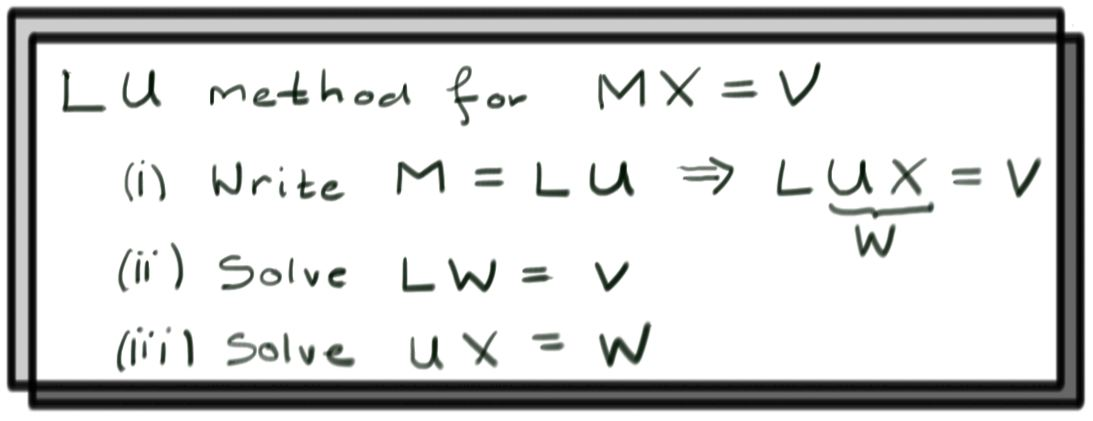
\includegraphics[scale=.3]{\luDecompPath/LU_solution.jpg}
\end{center}
%\end{figure}

\section{Finding an $LU$ Decomposition.}
\label{finding_LU_decomp}
 
For any given matrix, there are actually many different $LU$ decompositions.  However, there is a unique $LU$ decomposition in which the $L$ matrix has ones on the diagonal. In that case $L$ is called a \emph{lower unit triangular matrix}\index{Lower unit triangular matrix}.

To find the $LU$ decomposition, we'll create two sequences of matrices $L_0, L_1, \ldots$ and $U_0, U_1, \ldots$ such that at each step, $L_iU_i=M$.  Each of the $L_i$ will be lower triangular, but only the last $U_i$ will be upper triangular.

Start by setting $L_0=I$ and $U_0=M$, because $L_0U_0=M$. A main concept of this calculation is captured by the following example:

\begin{example}
Consider $$E=\begin{pmatrix}1&0\\\lambda&1\end{pmatrix}\, ,\qquad M=\begin{pmatrix}a&b&c&\cdots\\d&e&f&\cdots\end{pmatrix}\, .$$
Lets compute $EM$
$$
EM=\begin{pmatrix}a&b&c&\cdots\\d+\lambda a&e+\lambda b&f+\lambda c&\cdots\end{pmatrix}\, ,.
$$
Something neat happened here: multiplying $M$ by $E$ performed the row operation $R_2\to R_2+\lambda R-1$ on $M$.
Another interesting fact:
$$
E^{-1}:=\begin{pmatrix}1&0\\-\lambda&1\end{pmatrix}
$$ 
obeys (check this yourself...)
$$
E^{-1} E = 1\, .
$$
Hence $M=E^{-1} E M$ or, writing this out
$$
\begin{pmatrix}a&b&c&\cdots\\d&e&f&\cdots\end{pmatrix}=\begin{pmatrix}1&0\\-\lambda&1\end{pmatrix} \begin{pmatrix}a&b&c&\cdots\\d+\lambda a&e+\lambda b&f+\lambda c&\cdots\end{pmatrix}\, .
$$
Here the matrix on the left is lower triangular, while the matrix on the right has had a row operation performed on it.
\end{example}




\vspace{2mm}
We would like to  use the first row of $U_0$ to zero out the first entry of every row below it.  For our running example, $$U_0=M=\begin{pmatrix}
6 & 18 & 3 \\
2 & 12 & 1 \\
4 & 15 & 3 
\end{pmatrix}\, ,$$ so we would like to perform the row operations $R_2\to R_2 -\frac 13 R_1$ and $R_3\to R_3-\frac 23R_1$.
%so the second row minus $\frac{1}{3}$ of the first row will zero out the first entry in the second row.  Likewise, the third row minus $\frac{2}{3}$ of the first row will zero out the first entry in the third row.
If we perform these row operations on $U_0$ to produce 
$$U_1=\begin{pmatrix}
6 & 18 & 3 \\
0 & 6 & 0 \\
0 & 3 & 1 
\end{pmatrix}\, ,$$
we need to multiply this on the left by a lower triangular matrix $L_1$ so that the product $L_1U_1=M$ still.
The above example shows how to do this:
Set $L_1$ to be the lower triangular matrix whose first column is filled with the minus constants used to zero out the first column of $M$.  Then $$L_1 = \begin{pmatrix}
1 & 0 & 0 \\[1mm]
\frac{1}{3} & 1 & 0 \\[1mm]
\frac{2}{3} & 0 & 1 
\end{pmatrix}\, .$$  
%Set $U_1$ to be the matrix obtained by zeroing out the first column of $M$.  Then $U_1=\begin{pmatrix}
%6 & 18 & 3 \\
%0 & 6 & 0 \\
%0 & 3 & 1 
%\end{pmatrix}$.
By construction $L_1 U_1=M$, but you should compute this yourself as a double check.

Now repeat the process by zeroing the second column of $U_1$ below the diagonal using the second row of $U_1$ using the row operation
$R_3\to R_3-\frac 12 R_2$ to produce
$$U_2=\begin{pmatrix}6&18&3\\0&6&0\\0&0&1\end{pmatrix}\, .$$
The matrix that undoes this row operation is obtained in the same way we found $L_1$ above and is:
$$
\begin{pmatrix}
1&0&0\\
0&1&0\\
0&\frac 12& 0
\end{pmatrix}\, .
$$
Thus our answer for $L_2$ is the product of this matrix with $L_1$, namely
$$
L_2=
\begin{pmatrix}
1 & 0 & 0 \\[1mm]
\frac{1}{3} & 1 & 0 \\[1mm]
\frac{2}{3} & 0 & 1 
\end{pmatrix}\begin{pmatrix}
1&0&0\\
0&1&0\\
0&\frac 12& 0
\end{pmatrix}
=\begin{pmatrix}
1 & 0 & 0 \\[1mm]
\frac{1}{3} & 1 & 0 \\[1mm]
\frac{2}{3} & \frac{1}{2} & 1 
\end{pmatrix}\, .
$$
Notice that it is lower triangular because 

\begin{center}
\textcolor{brown}{THE PRODUCT OF LOWER TRIANGULAR MATRICES IS ALWAYS LOWER TRIANGULAR!}
\end{center}

\noindent
Moreover it is obtained by recording minus the constants used for all our row operations in the appropriate columns (this always works this way).
Moreover, $U_2$ is upper triangular and $M=L_2U_2$, we are done!
Putting this all together we have
$$M=\begin{pmatrix}
6 & 18 & 3 \\
2 & 12 & 1 \\
4 & 15 & 3 
\end{pmatrix}= \begin{pmatrix}
1 & 0 & 0 \\[1mm]
\frac{1}{3} & 1 & 0 \\[1mm]
\frac{2}{3} & \frac{1}{2} & 1 
\end{pmatrix}\begin{pmatrix}
6 & 18 & 3 \\
0 & 6 & 0 \\
0 & 0 & 1 
\end{pmatrix}\, .$$  
%Since $U_2$ is upper-triangular, we're done.  Inserting the new number into $L_1$ to get $L_2$ really is safe: the numbers in the first column don't affect the second column of $U_1$, since the first column of $U_1$ is already zeroed out.

If the matrix you're working with has more than three rows, just continue this process by zeroing out the next column below the diagonal, and repeat until there's nothing left to do.

\videoscriptlink{lu_decomposition_example.mp4}{Another $LU$ decomposition example}{scripts_lu_decomposition_example}

The fractions in the $L$ matrix are admittedly ugly.  For two matrices $LU$, we can multiply one entire column of $L$ by a constant $\lambda$ and divide the corresponding row of $U$ by the same constant without changing the product of the two matrices.  Then:

\begin{eqnarray*}
LU &=& \begin{pmatrix}
1 & 0 & 0 \\[1mm]
\frac{1}{3} & 1 & 0 \\[1mm]
\frac{2}{3} & \frac{1}{2} & 1 
\end{pmatrix}
I
\begin{pmatrix}
6 & 18 & 3 \\
0 & 6 & 0 \\
0 & 0 & 1 
\end{pmatrix} \\
&=&
\begin{pmatrix}
1 & 0 & 0 \\[1mm]
\frac{1}{3} & 1 & 0 \\[1mm]
\frac{2}{3} & \frac{1}{2} & 1 
\end{pmatrix}
\begin{pmatrix}
3 & 0 & 0 \\
0 & 6 & 0 \\
0 & 0 & 1 
\end{pmatrix}
\begin{pmatrix}
\frac{1}{3} & 0 & 0 \\[1mm]
0 & \frac{1}{6} & 0 \\[1mm]
0 & 0 & 1 
\end{pmatrix}
\begin{pmatrix}
6 & 18 & 3 \\
0 & 6 & 0 \\
0 & 0 & 1 
\end{pmatrix} \\
&=&
\begin{pmatrix}
3 & 0 & 0 \\
1 & 6 & 0 \\
2 & 3 & 1 
\end{pmatrix}\begin{pmatrix}
2 & 6 & 1 \\
0 & 1 & 0 \\
0 & 0 & 1 
\end{pmatrix}.
\end{eqnarray*}
The resulting matrix looks nicer, but isn't in standard (lower unit triangular matrix) form.

\reading{11}{2}
%\href{\webworkurl ReadingHomework11/2/}{Reading homework: problem 11.2}

For matrices that are not square, $LU$ decomposition still makes sense.  Given an $m\times n$ matrix $M$, for example we could write $M=LU$ with $L$ a square lower unit triangular matrix, and $U$ a rectangular matrix.  Then $L$ will be an $m\times m$ matrix, and $U$ will be an $m\times n$ matrix (of the same shape as $M$).  From here, the process is exactly the same as for a square matrix.  We create a sequence of matrices $L_i$ and $U_i$ that is eventually the $LU$ decomposition.  Again, we start with $L_0=I$ and $U_0=M$.

\begin{example}
Let's find the $LU$ decomposition of $M=U_0=\begin{pmatrix}
-2 & 1 & 3 \\
-4 & 4 & 1 
\end{pmatrix}$.  Since $M$ is a $2\times 3$ matrix, our decomposition will consist of a $2\times 2$ matrix and a $2\times 3$ matrix.  Then we start with $L_0=I_2=\begin{pmatrix}
1 & 0 \\
0 & 1
\end{pmatrix}$.

The next step is to zero-out the first column of $M$ below the diagonal.  There is only one row to cancel, then, and it can be removed by subtracting $2$ times the first row of $M$ to the second row of $M$.  Then:

\[
L_1=\begin{pmatrix}
1 & 0 \\
2 & 1
\end{pmatrix}, \qquad 
U_1 = \begin{pmatrix}
-2 & 1 & 3 \\
0 & 2 & -5 
\end{pmatrix}
\]
Since $U_1$ is upper triangular, we're done.  With a larger matrix, we would just continue the process.
\end{example}





\section{Block $LDU$ Decomposition}

Let $M$ be a square block matrix with square blocks $X,Y,Z,W$ such that $X^{-1}$ exists.  Then $M$ can be decomposed as a block $LDU$ decomposition, where $D$ is block diagonal, as follows:
\[
M=\begin{pmatrix}
X & Y \\
Z & W
\end{pmatrix}
\]

Then: \[M=\begin{pmatrix}
I &  0 \\
ZX^{-1} & I
\end{pmatrix}\begin{pmatrix}
X & 0 \\
0 & W-ZX^{-1}Y
\end{pmatrix}\begin{pmatrix}
I & X^{-1}Y \\
0 & I
\end{pmatrix}.\]
This can be checked explicitly simply by block-multiplying these three matrices.

\videoscriptlink{lu_decomposition_blocks.mp4}{Block $LDU$ Explanation}{scripts_lu_decomposition_blocks}

\begin{example}
For a $2\times 2$ matrix, we can regard each entry as a block.
\[
\begin{pmatrix}
1 & 2 \\
3 & 4
\end{pmatrix}=
\begin{pmatrix}
1 & 0 \\
3 & 1
\end{pmatrix}
\begin{pmatrix}
1 & 0 \\
0 & -2
\end{pmatrix}
\begin{pmatrix}
1 & 2 \\
0 & 1
\end{pmatrix}
\]
By multiplying the diagonal matrix by the upper triangular matrix, we get the standard $LU$ decomposition of the matrix.
\end{example}


%\section*{References}
%Wikipedia:
%\begin{itemize}
%\item \href{http://en.wikipedia.org/wiki/LU_decomposition}{$LU$ Decomposition}
%\item \href{http://en.wikipedia.org/wiki/Block_LU_decomposition}{Block $LU$ Decomposition}
%\end{itemize}

\section{Review Problems}



\begin{enumerate}

\item Let $D=\begin{pmatrix}
\lambda_1 & \mc0 \\
\mc0 & \lambda_2 \\
\end{pmatrix}$.
\begin{enumerate}
\item Write $D$ in terms of the vectors $e_1$ and $e_2$, and their transposes.
\item Suppose $P=\begin{pmatrix}
a & b \\
c & d \\
\end{pmatrix}$ is invertible.  Show that $D$ is similar to
\[
M=\frac{1}{ad-bc}\begin{pmatrix}
\lambda_1ad-\lambda_2bc & -(\lambda_1-\lambda_2)ab \\[1mm]
(\lambda_1-\lambda_2)cd & -\lambda_1bc + \lambda_2ad
\end{pmatrix}.
\]
\item Suppose the vectors $\rowvec{a,b}$ and $\rowvec{c,d}$ are orthogonal.  What can you say about $M$ in this case? (Hint: think about what \(M^T\) is equal to.)
\end{enumerate}

\phantomnewpage

\item \label{orthogprob} Suppose $S=\{v_1, \ldots, v_n \}$ is an \emph{orthogonal} (not orthonormal) basis for~$\Re^n$.  Then we can write any vector $v$ as $v=\sum_ic^iv_i$ for some constants $c^i$.  Find a formula for the constants $c^i$ in terms of $v$ and the vectors in~$S$.

\Videoscriptlink{orthonormal_bases_hint.mp4}{Hint}{scripts_orthonormal_bases_hint}
\phantomnewpage

\item \label{orthogprojprob} Let $u,v$ be linearly independent vectors in $\Re^3$, and $P=\spa \{ u,v\}$ be the plane spanned by $u$ and $v$.  
\begin{enumerate}
\item Is the vector $v^\bot := v-\frac{u\cdot v}{u\cdot u}u$ in the plane $P$?
\item  What is the (cosine of the) angle between $v^\bot$ and $u$?
\item %Given your solution to the above, 
How can you find a third vector perpendicular to both $u$ and $v^\bot$?
\item  Construct an orthonormal basis for $\Re^3$ from $u$ and $v$.
\item  Test your abstract formul\ae\ starting with 
\[
u=\rowvec{1 , 2 , 0} \text{ and } v=\rowvec{0 , 1 , 1}.
\]
\end{enumerate}

\Videoscriptlink{orthonormal_bases_hint3.mp4}{Hint}{scripts_orthonormal_bases_hint3}

\phantomnewpage



\item Find an orthonormal  basis for $\Re^4$ which includes $(1,1,1,1)$ using the following procedure:\\
\begin{enumerate} 
\item Pick a vector perpendicular to the vector 
$$v_1 =\colvec{1\\1\\1\\1}$$ from the solution set of the matrix equation $$v_1^Tx=0\, .$$ Pick the vector $v_2$ obtained from the standard Gaussian elimination procedure which is the coefficient of $x_2$.
\item Pick a vector perpendicular to both $v_1$ and $v_2$ from the solutions set of the matrix equation $$\colvec{v_1^T\\[1mm]v_2^T}x=0\, .$$ Pick the vector $v_3$ obtained from the standard Gaussian elimination procedure with $x_3$ as the coefficient. 
\item Pick a vector perpendicular to $v_1,v_2,$ and $v_3$ from the solution set of the matrix equation $$\colvec{v_1^T\\[1mm]v_2^T\\[1mm]v_3^T}x=0\, .$$  Pick the vector $v_4$ obtained from the standard Gaussian elimination procedure with $x_3$ as the coefficient. 
\item Normalize the four vectors obtained   above.
\end{enumerate}


\item Use the inner product $$f\cdot g := \int_0^1 f(x)g(x)dx$$  on the vector space $V={\rm span} \{1,x,x^2,x^3\}$ to perform the Gram-Schmidt procedure on the set of vectors $\{1,x,x^2,x^3\}$. 

\item Use the inner product $$f\cdot g := \int_0^{2\pi} f(x)g(x)dx$$  on the vector space $V={\rm span} \{\sin(x),\sin(2x),\sin(3x) \}$ to perform the Gram-Schmidt procedure on the set of vectors $\{\sin(x),\sin(2x),\sin(3x) \}$. \\
Try to build an orthonormal basis for the vector space $$\spa \{ \sin(nx)~| ~n\in \N \}\, .$$
%What do you suspect about the vector space $\spa \{ \sin(nx)~| ~n\in \N \}$?\\
%What do you suspect about the vector space $\spa \{ \sin(ax)~|~ a \in \Re \}$?
\item 
\begin{enumerate}
\item
Show that if $Q$ is an orthogonal $n\times n$ matrix, then $$u\dotprod v = (Qu)\dotprod (Qv)\, ,$$ for any $u,v\in \Re^n$. That is, $Q$ preserves the inner product. 
\item Does $Q$ preserve the outer product? 
\item  If the set of vectors $\{ u_1,\dots,u_n\}$ is orthonormal and $\{ \lambda_1,\cdots,\lambda_n\}$ is a set of numbers, 
then what are the eigenvalues and eigenvectors of the matrix
$M=\sum_{i=1}^n \lambda_i u_i u_i^T$? 
\item How would the eigenvectors and eigenvalues of this matrix change if we replaced  $\{ u_1,\dots,u_n\}$ by $\{ Qu_1,\dots,Q u_n\}$?
\end{enumerate}


\item Carefully write out the Gram-Schmidt procedure for the set of vectors 
$$\left\{ \colvec{1\\1\\1}, \colvec{1\\-1\\1}, \colvec{1\\1\\-1} \right\} \, .$$ Is it possible to rescale the second vector obtained in the procedure to a vector with integer components? 


\item 
\label{basisortho}
\begin{enumerate}
\item Suppose $u$ and $v$ are linearly independent.  Show that $u$ and $v^\perp$ are also linearly independent.  Explain why $\{u, v^\perp\}$ is a basis for $\spa \{u,v\}$.



\Videoscriptlink{gram_schmidt_and_orthogonal_complements_hint.mp4}{Hint}{gram_schmidt_and_orthogonal_complements_hint}

\item Repeat the previous problem, but with three independent vectors $u,v,w$
 where $v^\perp$ and $w^\perp$ are as defined by the Gram-Schmidt procedure. 
\end{enumerate}

\phantomnewpage


\item \label{QRprob} Find the $QR$ factorization of
$$
M=\begin{pmatrix}1&0&\phantom{\!-}2\\-1&2&0\\-1&-2&2
\end{pmatrix}\, .
$$

\phantomnewpage

\item Given any three vectors $u,v,w$, when do $v^\perp$ or $w^\perp$ of the Gram--Schmidt procedure vanish?

\phantomnewpage

\item For $U$ a subspace of $W$, use the subspace theorem to check that $U^\perp$ is a subspace of $W$.

\phantomnewpage


\phantomnewpage

\item %(Extra Credit) 
Let $S_n$ and $A_n$ define the space of $n \times n$ symmetric and anti-symmetric matrices, respectively. These are subspaces of the vector space $M^n_n$ of all $n\times n$ matrices. What is $\dim M^n_n$, $\dim S_n$, and $\dim A_n$? Show that $M^n_n = S_n + A_n$. Define an inner product on square matrices
$$
M\cdot N ={\rm tr} MN\, .
$$
Is $A_n^{\perp}=S_n$? Is $M^n_n = S_n \oplus A_n$?

%\emph{Hint: Note that $\dim S_n = \dim U_n$ where $U_n$ is the vector space of all $n \times n$ upper triangular matrices, and also note that $\dim A_n = \dim \widetilde{U}_n$ where $\widetilde{U}_n$ is the vector space of all strictly $n \times n$ upper triangular matrices (\emph{i.e.} the diagonal entries are all 0).}

\item The vector space $V={\rm span} \{ \sin(t),\sin(2t), \sin(3t) , \sin(3t)\}$ has an inner product: 
$$f\cdot g:=\int _0^{2\pi}f(t)g(t) dt\, .$$ Find the orthogonal compliment to $U={\rm span} \{ \sin(t)+\sin(2t) \}$ in $V$. Express $\sin(t)-\sin(2t)$ as  the sum of vectors from $U$ and $U^\perp$.

\end{enumerate}

\phantomnewpage

\newpage


\chapter{\luDecompTitle}
\label{LUdecomp}

Certain matrices are easier to work with than others.  In this section, we will see how to write any square\footnote{The case where $M$ is not square is dealt with at the end of the lecture.} matrix $M$ as the product of two simpler matrices.  We will write $$M=LU\, ,$$ where:
\begin{itemize}
\item $L$ is \emph{lower triangular}\index{Lower triangular matrix}.  This means that all entries above the main diagonal are zero.  In notation,
$L=(l^i_j)$ with $l^i_j=0$ for all $j>i$.
\[L=\begin{pmatrix}
l^1_1 & 0 & 0 & \cdots \\
l^2_1 & l^2_2 & 0 & \cdots \\
l^3_1 & l^3_2 & l^3_3 & \cdots \\
\vdots & \vdots & \vdots & \ddots \\
\end{pmatrix}
\]

\item $U$ is \emph{upper triangular}\index{Upper triangular matrix}.  This means that all entries below the main diagonal are zero.  In notation,
$U=(u^i_j)$ with $u^i_j=0$ for all $j<i$.
\[U=\begin{pmatrix}
u^1_1 & u^1_2 & u^1_3 & \cdots \\
0 & u^2_2 & u^2_3 & \cdots \\
0 & 0 & u^3_3 & \cdots \\
\vdots & \vdots & \vdots & \ddots \\
\end{pmatrix}
\]
\end{itemize}
$M=LU$ is called an \emph{$LU$ decomposition}\index{LU@$LU$ decomposition} of $M$.

This is a useful trick for  computational reasons; it is much easier to compute the inverse of an upper or lower triangular matrix than general matrices.  Since inverses are useful for solving linear systems, this makes solving any linear system associated to the matrix much faster as well.  The determinant---a very important quantity associated with any square matrix---is very easy to compute for triangular matrices.

\begin{example}
Linear systems associated to upper triangular matrices are very easy to solve by back substitution.
\[
\begin{amatrix}{2}
a & b & 1 \\
0 & c & e \\
\end{amatrix} \ \Rightarrow \ y=\frac{e}{c}\, , \quad x=\frac{1}{a}\left(1-\frac{be}{c}\right)
\]

\[
\begin{amatrix}{3}
1 & 0 & 0 & d \\
a & 1 & 0 & e \\
b & c & 1 & f \\
\end{amatrix} \Rightarrow x=d\, , \qquad y=e-ad\, , \qquad z=f-bd-c(e-ad)
\]
For lower triangular matrices, \emph{back} substitution\index{Back substitution} gives a quick solution; for upper triangular matrices, \emph{forward} substitution\index{Forward substitution} gives the solution.
\end{example}





\section{Using $LU$ Decomposition to Solve Linear Systems}

Suppose we have $M=LU$ and want to solve the system
\[
MX=LUX=V.
\]

\begin{itemize}
\item{Step 1:} Set $W=\colvec{u\\v\\w}=UX$.  

\item{Step 2:} Solve the system $LW=V$.  This should be simple by forward substitution since $L$ is lower triangular.  Suppose the solution to $LW=V$ is $W_0$.  

\item{Step 3:} Now solve the system $UX=W_0$.  This should be easy by backward substitution, since $U$ is upper triangular.  The solution to this system is the solution to the original system.
\end{itemize}
We can think of this as using the matrix $L$ to perform row operations on the matrix $U$ in order to solve the system; this idea also appears in the  study of determinants.

%\href{\webworkurl ReadingHomework11/1/}{Reading homework: problem 11.1}
\reading{11}{1}

\begin{example}
Consider the linear system:
\[
      \begin{linsys}{4}
            6x & +&18y & +&3z         &=& 3  \\[1mm]
            2x & +&12y & +&z	    &=& 19 \\[1mm]
            4x & +&15y & +&3z         &=& 0  
      \end{linsys}
\]

An $LU$ decomposition for the associated matrix $M$ is:
\[
\begin{pmatrix}
6 & 18 & 3 \\
2 & 12 & 1 \\
4 & 15 & 3 
\end{pmatrix} =
\begin{pmatrix}
3 & 0 & 0 \\
1 & 6 & 0 \\
2 & 3 & 1 
\end{pmatrix}
\begin{pmatrix}
2 & 6 & 1 \\
0 & 1 & 0 \\
0 & 0 & 1 
\end{pmatrix}.
\]

\begin{itemize}
\item{Step 1:} \hypertarget{LUproc}{Set} $W=\colvec{u\\v\\w}=UX$.  

\item{Step 2:} Solve the system $LW=V$:

\[
\begin{pmatrix}
3 & 0 & 0 \\
1 & 6 & 0 \\
2 & 3 & 1 
\end{pmatrix}
\colvec{u\\v\\w} =
\colvec{3\\19\\0}
\]

By substitution, we get $u=1$, $v=3$, and $w=-11$.  Then 
\[W_0=\colvec{1\\3\\-11}\]

\item{Step 3:} Solve the system $UX=W_0$.  
\[
\begin{pmatrix}
2 & 6 & 1 \\
0 & 1 & 0 \\
0 & 0 & 1 
\end{pmatrix}
\colvec{x\\y\\z} =
\colvec{1\\3\\-11}
\]
Back substitution gives $z=-11, y=3$, and $x=-3$.  

Then $X=\colvec{-3\\3\\-11}$, and we're done.
\end{itemize}
\end{example}

\videoscriptlink{lu_decomposition_using_lu_decomp.mp4}{Using a $LU$ decomposition}{scripts_lu_decomposition_using_lu_example}

%\begin{figure}
\begin{center}
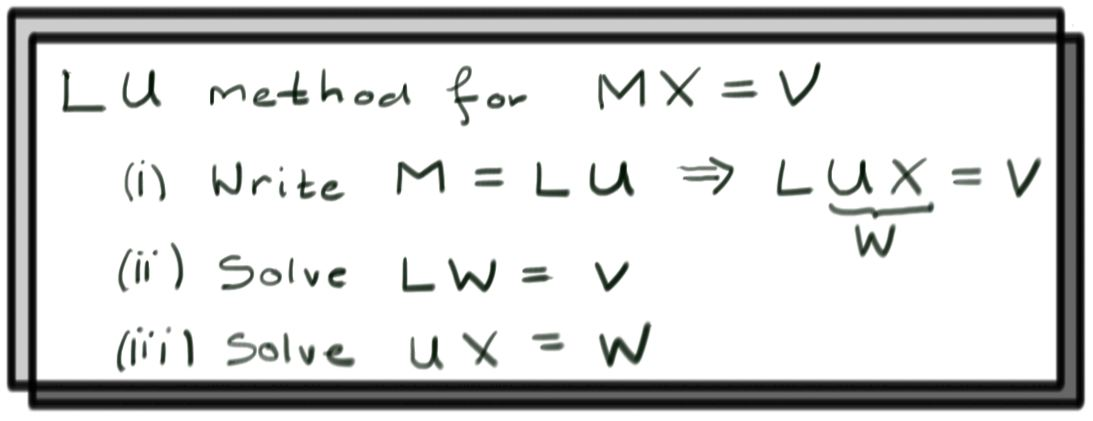
\includegraphics[scale=.3]{\luDecompPath/LU_solution.jpg}
\end{center}
%\end{figure}

\section{Finding an $LU$ Decomposition.}
\label{finding_LU_decomp}
 
For any given matrix, there are actually many different $LU$ decompositions.  However, there is a unique $LU$ decomposition in which the $L$ matrix has ones on the diagonal. In that case $L$ is called a \emph{lower unit triangular matrix}\index{Lower unit triangular matrix}.

To find the $LU$ decomposition, we'll create two sequences of matrices $L_0, L_1, \ldots$ and $U_0, U_1, \ldots$ such that at each step, $L_iU_i=M$.  Each of the $L_i$ will be lower triangular, but only the last $U_i$ will be upper triangular.

Start by setting $L_0=I$ and $U_0=M$, because $L_0U_0=M$. A main concept of this calculation is captured by the following example:

\begin{example}
Consider $$E=\begin{pmatrix}1&0\\\lambda&1\end{pmatrix}\, ,\qquad M=\begin{pmatrix}a&b&c&\cdots\\d&e&f&\cdots\end{pmatrix}\, .$$
Lets compute $EM$
$$
EM=\begin{pmatrix}a&b&c&\cdots\\d+\lambda a&e+\lambda b&f+\lambda c&\cdots\end{pmatrix}\, ,.
$$
Something neat happened here: multiplying $M$ by $E$ performed the row operation $R_2\to R_2+\lambda R-1$ on $M$.
Another interesting fact:
$$
E^{-1}:=\begin{pmatrix}1&0\\-\lambda&1\end{pmatrix}
$$ 
obeys (check this yourself...)
$$
E^{-1} E = 1\, .
$$
Hence $M=E^{-1} E M$ or, writing this out
$$
\begin{pmatrix}a&b&c&\cdots\\d&e&f&\cdots\end{pmatrix}=\begin{pmatrix}1&0\\-\lambda&1\end{pmatrix} \begin{pmatrix}a&b&c&\cdots\\d+\lambda a&e+\lambda b&f+\lambda c&\cdots\end{pmatrix}\, .
$$
Here the matrix on the left is lower triangular, while the matrix on the right has had a row operation performed on it.
\end{example}




\vspace{2mm}
We would like to  use the first row of $U_0$ to zero out the first entry of every row below it.  For our running example, $$U_0=M=\begin{pmatrix}
6 & 18 & 3 \\
2 & 12 & 1 \\
4 & 15 & 3 
\end{pmatrix}\, ,$$ so we would like to perform the row operations $R_2\to R_2 -\frac 13 R_1$ and $R_3\to R_3-\frac 23R_1$.
%so the second row minus $\frac{1}{3}$ of the first row will zero out the first entry in the second row.  Likewise, the third row minus $\frac{2}{3}$ of the first row will zero out the first entry in the third row.
If we perform these row operations on $U_0$ to produce 
$$U_1=\begin{pmatrix}
6 & 18 & 3 \\
0 & 6 & 0 \\
0 & 3 & 1 
\end{pmatrix}\, ,$$
we need to multiply this on the left by a lower triangular matrix $L_1$ so that the product $L_1U_1=M$ still.
The above example shows how to do this:
Set $L_1$ to be the lower triangular matrix whose first column is filled with the minus constants used to zero out the first column of $M$.  Then $$L_1 = \begin{pmatrix}
1 & 0 & 0 \\[1mm]
\frac{1}{3} & 1 & 0 \\[1mm]
\frac{2}{3} & 0 & 1 
\end{pmatrix}\, .$$  
%Set $U_1$ to be the matrix obtained by zeroing out the first column of $M$.  Then $U_1=\begin{pmatrix}
%6 & 18 & 3 \\
%0 & 6 & 0 \\
%0 & 3 & 1 
%\end{pmatrix}$.
By construction $L_1 U_1=M$, but you should compute this yourself as a double check.

Now repeat the process by zeroing the second column of $U_1$ below the diagonal using the second row of $U_1$ using the row operation
$R_3\to R_3-\frac 12 R_2$ to produce
$$U_2=\begin{pmatrix}6&18&3\\0&6&0\\0&0&1\end{pmatrix}\, .$$
The matrix that undoes this row operation is obtained in the same way we found $L_1$ above and is:
$$
\begin{pmatrix}
1&0&0\\
0&1&0\\
0&\frac 12& 0
\end{pmatrix}\, .
$$
Thus our answer for $L_2$ is the product of this matrix with $L_1$, namely
$$
L_2=
\begin{pmatrix}
1 & 0 & 0 \\[1mm]
\frac{1}{3} & 1 & 0 \\[1mm]
\frac{2}{3} & 0 & 1 
\end{pmatrix}\begin{pmatrix}
1&0&0\\
0&1&0\\
0&\frac 12& 0
\end{pmatrix}
=\begin{pmatrix}
1 & 0 & 0 \\[1mm]
\frac{1}{3} & 1 & 0 \\[1mm]
\frac{2}{3} & \frac{1}{2} & 1 
\end{pmatrix}\, .
$$
Notice that it is lower triangular because 

\begin{center}
\textcolor{brown}{THE PRODUCT OF LOWER TRIANGULAR MATRICES IS ALWAYS LOWER TRIANGULAR!}
\end{center}

\noindent
Moreover it is obtained by recording minus the constants used for all our row operations in the appropriate columns (this always works this way).
Moreover, $U_2$ is upper triangular and $M=L_2U_2$, we are done!
Putting this all together we have
$$M=\begin{pmatrix}
6 & 18 & 3 \\
2 & 12 & 1 \\
4 & 15 & 3 
\end{pmatrix}= \begin{pmatrix}
1 & 0 & 0 \\[1mm]
\frac{1}{3} & 1 & 0 \\[1mm]
\frac{2}{3} & \frac{1}{2} & 1 
\end{pmatrix}\begin{pmatrix}
6 & 18 & 3 \\
0 & 6 & 0 \\
0 & 0 & 1 
\end{pmatrix}\, .$$  
%Since $U_2$ is upper-triangular, we're done.  Inserting the new number into $L_1$ to get $L_2$ really is safe: the numbers in the first column don't affect the second column of $U_1$, since the first column of $U_1$ is already zeroed out.

If the matrix you're working with has more than three rows, just continue this process by zeroing out the next column below the diagonal, and repeat until there's nothing left to do.

\videoscriptlink{lu_decomposition_example.mp4}{Another $LU$ decomposition example}{scripts_lu_decomposition_example}

The fractions in the $L$ matrix are admittedly ugly.  For two matrices $LU$, we can multiply one entire column of $L$ by a constant $\lambda$ and divide the corresponding row of $U$ by the same constant without changing the product of the two matrices.  Then:

\begin{eqnarray*}
LU &=& \begin{pmatrix}
1 & 0 & 0 \\[1mm]
\frac{1}{3} & 1 & 0 \\[1mm]
\frac{2}{3} & \frac{1}{2} & 1 
\end{pmatrix}
I
\begin{pmatrix}
6 & 18 & 3 \\
0 & 6 & 0 \\
0 & 0 & 1 
\end{pmatrix} \\
&=&
\begin{pmatrix}
1 & 0 & 0 \\[1mm]
\frac{1}{3} & 1 & 0 \\[1mm]
\frac{2}{3} & \frac{1}{2} & 1 
\end{pmatrix}
\begin{pmatrix}
3 & 0 & 0 \\
0 & 6 & 0 \\
0 & 0 & 1 
\end{pmatrix}
\begin{pmatrix}
\frac{1}{3} & 0 & 0 \\[1mm]
0 & \frac{1}{6} & 0 \\[1mm]
0 & 0 & 1 
\end{pmatrix}
\begin{pmatrix}
6 & 18 & 3 \\
0 & 6 & 0 \\
0 & 0 & 1 
\end{pmatrix} \\
&=&
\begin{pmatrix}
3 & 0 & 0 \\
1 & 6 & 0 \\
2 & 3 & 1 
\end{pmatrix}\begin{pmatrix}
2 & 6 & 1 \\
0 & 1 & 0 \\
0 & 0 & 1 
\end{pmatrix}.
\end{eqnarray*}
The resulting matrix looks nicer, but isn't in standard (lower unit triangular matrix) form.

\reading{11}{2}
%\href{\webworkurl ReadingHomework11/2/}{Reading homework: problem 11.2}

For matrices that are not square, $LU$ decomposition still makes sense.  Given an $m\times n$ matrix $M$, for example we could write $M=LU$ with $L$ a square lower unit triangular matrix, and $U$ a rectangular matrix.  Then $L$ will be an $m\times m$ matrix, and $U$ will be an $m\times n$ matrix (of the same shape as $M$).  From here, the process is exactly the same as for a square matrix.  We create a sequence of matrices $L_i$ and $U_i$ that is eventually the $LU$ decomposition.  Again, we start with $L_0=I$ and $U_0=M$.

\begin{example}
Let's find the $LU$ decomposition of $M=U_0=\begin{pmatrix}
-2 & 1 & 3 \\
-4 & 4 & 1 
\end{pmatrix}$.  Since $M$ is a $2\times 3$ matrix, our decomposition will consist of a $2\times 2$ matrix and a $2\times 3$ matrix.  Then we start with $L_0=I_2=\begin{pmatrix}
1 & 0 \\
0 & 1
\end{pmatrix}$.

The next step is to zero-out the first column of $M$ below the diagonal.  There is only one row to cancel, then, and it can be removed by subtracting $2$ times the first row of $M$ to the second row of $M$.  Then:

\[
L_1=\begin{pmatrix}
1 & 0 \\
2 & 1
\end{pmatrix}, \qquad 
U_1 = \begin{pmatrix}
-2 & 1 & 3 \\
0 & 2 & -5 
\end{pmatrix}
\]
Since $U_1$ is upper triangular, we're done.  With a larger matrix, we would just continue the process.
\end{example}





\section{Block $LDU$ Decomposition}

Let $M$ be a square block matrix with square blocks $X,Y,Z,W$ such that $X^{-1}$ exists.  Then $M$ can be decomposed as a block $LDU$ decomposition, where $D$ is block diagonal, as follows:
\[
M=\begin{pmatrix}
X & Y \\
Z & W
\end{pmatrix}
\]

Then: \[M=\begin{pmatrix}
I &  0 \\
ZX^{-1} & I
\end{pmatrix}\begin{pmatrix}
X & 0 \\
0 & W-ZX^{-1}Y
\end{pmatrix}\begin{pmatrix}
I & X^{-1}Y \\
0 & I
\end{pmatrix}.\]
This can be checked explicitly simply by block-multiplying these three matrices.

\videoscriptlink{lu_decomposition_blocks.mp4}{Block $LDU$ Explanation}{scripts_lu_decomposition_blocks}

\begin{example}
For a $2\times 2$ matrix, we can regard each entry as a block.
\[
\begin{pmatrix}
1 & 2 \\
3 & 4
\end{pmatrix}=
\begin{pmatrix}
1 & 0 \\
3 & 1
\end{pmatrix}
\begin{pmatrix}
1 & 0 \\
0 & -2
\end{pmatrix}
\begin{pmatrix}
1 & 2 \\
0 & 1
\end{pmatrix}
\]
By multiplying the diagonal matrix by the upper triangular matrix, we get the standard $LU$ decomposition of the matrix.
\end{example}


%\section*{References}
%Wikipedia:
%\begin{itemize}
%\item \href{http://en.wikipedia.org/wiki/LU_decomposition}{$LU$ Decomposition}
%\item \href{http://en.wikipedia.org/wiki/Block_LU_decomposition}{Block $LU$ Decomposition}
%\end{itemize}

\section{Review Problems}



\begin{enumerate}

\item Let $D=\begin{pmatrix}
\lambda_1 & \mc0 \\
\mc0 & \lambda_2 \\
\end{pmatrix}$.
\begin{enumerate}
\item Write $D$ in terms of the vectors $e_1$ and $e_2$, and their transposes.
\item Suppose $P=\begin{pmatrix}
a & b \\
c & d \\
\end{pmatrix}$ is invertible.  Show that $D$ is similar to
\[
M=\frac{1}{ad-bc}\begin{pmatrix}
\lambda_1ad-\lambda_2bc & -(\lambda_1-\lambda_2)ab \\[1mm]
(\lambda_1-\lambda_2)cd & -\lambda_1bc + \lambda_2ad
\end{pmatrix}.
\]
\item Suppose the vectors $\rowvec{a,b}$ and $\rowvec{c,d}$ are orthogonal.  What can you say about $M$ in this case? (Hint: think about what \(M^T\) is equal to.)
\end{enumerate}

\phantomnewpage

\item \label{orthogprob} Suppose $S=\{v_1, \ldots, v_n \}$ is an \emph{orthogonal} (not orthonormal) basis for~$\Re^n$.  Then we can write any vector $v$ as $v=\sum_ic^iv_i$ for some constants $c^i$.  Find a formula for the constants $c^i$ in terms of $v$ and the vectors in~$S$.

\Videoscriptlink{orthonormal_bases_hint.mp4}{Hint}{scripts_orthonormal_bases_hint}
\phantomnewpage

\item \label{orthogprojprob} Let $u,v$ be linearly independent vectors in $\Re^3$, and $P=\spa \{ u,v\}$ be the plane spanned by $u$ and $v$.  
\begin{enumerate}
\item Is the vector $v^\bot := v-\frac{u\cdot v}{u\cdot u}u$ in the plane $P$?
\item  What is the (cosine of the) angle between $v^\bot$ and $u$?
\item %Given your solution to the above, 
How can you find a third vector perpendicular to both $u$ and $v^\bot$?
\item  Construct an orthonormal basis for $\Re^3$ from $u$ and $v$.
\item  Test your abstract formul\ae\ starting with 
\[
u=\rowvec{1 , 2 , 0} \text{ and } v=\rowvec{0 , 1 , 1}.
\]
\end{enumerate}

\Videoscriptlink{orthonormal_bases_hint3.mp4}{Hint}{scripts_orthonormal_bases_hint3}

\phantomnewpage



\item Find an orthonormal  basis for $\Re^4$ which includes $(1,1,1,1)$ using the following procedure:\\
\begin{enumerate} 
\item Pick a vector perpendicular to the vector 
$$v_1 =\colvec{1\\1\\1\\1}$$ from the solution set of the matrix equation $$v_1^Tx=0\, .$$ Pick the vector $v_2$ obtained from the standard Gaussian elimination procedure which is the coefficient of $x_2$.
\item Pick a vector perpendicular to both $v_1$ and $v_2$ from the solutions set of the matrix equation $$\colvec{v_1^T\\[1mm]v_2^T}x=0\, .$$ Pick the vector $v_3$ obtained from the standard Gaussian elimination procedure with $x_3$ as the coefficient. 
\item Pick a vector perpendicular to $v_1,v_2,$ and $v_3$ from the solution set of the matrix equation $$\colvec{v_1^T\\[1mm]v_2^T\\[1mm]v_3^T}x=0\, .$$  Pick the vector $v_4$ obtained from the standard Gaussian elimination procedure with $x_3$ as the coefficient. 
\item Normalize the four vectors obtained   above.
\end{enumerate}


\item Use the inner product $$f\cdot g := \int_0^1 f(x)g(x)dx$$  on the vector space $V={\rm span} \{1,x,x^2,x^3\}$ to perform the Gram-Schmidt procedure on the set of vectors $\{1,x,x^2,x^3\}$. 

\item Use the inner product $$f\cdot g := \int_0^{2\pi} f(x)g(x)dx$$  on the vector space $V={\rm span} \{\sin(x),\sin(2x),\sin(3x) \}$ to perform the Gram-Schmidt procedure on the set of vectors $\{\sin(x),\sin(2x),\sin(3x) \}$. \\
Try to build an orthonormal basis for the vector space $$\spa \{ \sin(nx)~| ~n\in \N \}\, .$$
%What do you suspect about the vector space $\spa \{ \sin(nx)~| ~n\in \N \}$?\\
%What do you suspect about the vector space $\spa \{ \sin(ax)~|~ a \in \Re \}$?
\item 
\begin{enumerate}
\item
Show that if $Q$ is an orthogonal $n\times n$ matrix, then $$u\dotprod v = (Qu)\dotprod (Qv)\, ,$$ for any $u,v\in \Re^n$. That is, $Q$ preserves the inner product. 
\item Does $Q$ preserve the outer product? 
\item  If the set of vectors $\{ u_1,\dots,u_n\}$ is orthonormal and $\{ \lambda_1,\cdots,\lambda_n\}$ is a set of numbers, 
then what are the eigenvalues and eigenvectors of the matrix
$M=\sum_{i=1}^n \lambda_i u_i u_i^T$? 
\item How would the eigenvectors and eigenvalues of this matrix change if we replaced  $\{ u_1,\dots,u_n\}$ by $\{ Qu_1,\dots,Q u_n\}$?
\end{enumerate}


\item Carefully write out the Gram-Schmidt procedure for the set of vectors 
$$\left\{ \colvec{1\\1\\1}, \colvec{1\\-1\\1}, \colvec{1\\1\\-1} \right\} \, .$$ Is it possible to rescale the second vector obtained in the procedure to a vector with integer components? 


\item 
\label{basisortho}
\begin{enumerate}
\item Suppose $u$ and $v$ are linearly independent.  Show that $u$ and $v^\perp$ are also linearly independent.  Explain why $\{u, v^\perp\}$ is a basis for $\spa \{u,v\}$.



\Videoscriptlink{gram_schmidt_and_orthogonal_complements_hint.mp4}{Hint}{gram_schmidt_and_orthogonal_complements_hint}

\item Repeat the previous problem, but with three independent vectors $u,v,w$
 where $v^\perp$ and $w^\perp$ are as defined by the Gram-Schmidt procedure. 
\end{enumerate}

\phantomnewpage


\item \label{QRprob} Find the $QR$ factorization of
$$
M=\begin{pmatrix}1&0&\phantom{\!-}2\\-1&2&0\\-1&-2&2
\end{pmatrix}\, .
$$

\phantomnewpage

\item Given any three vectors $u,v,w$, when do $v^\perp$ or $w^\perp$ of the Gram--Schmidt procedure vanish?

\phantomnewpage

\item For $U$ a subspace of $W$, use the subspace theorem to check that $U^\perp$ is a subspace of $W$.

\phantomnewpage


\phantomnewpage

\item %(Extra Credit) 
Let $S_n$ and $A_n$ define the space of $n \times n$ symmetric and anti-symmetric matrices, respectively. These are subspaces of the vector space $M^n_n$ of all $n\times n$ matrices. What is $\dim M^n_n$, $\dim S_n$, and $\dim A_n$? Show that $M^n_n = S_n + A_n$. Define an inner product on square matrices
$$
M\cdot N ={\rm tr} MN\, .
$$
Is $A_n^{\perp}=S_n$? Is $M^n_n = S_n \oplus A_n$?

%\emph{Hint: Note that $\dim S_n = \dim U_n$ where $U_n$ is the vector space of all $n \times n$ upper triangular matrices, and also note that $\dim A_n = \dim \widetilde{U}_n$ where $\widetilde{U}_n$ is the vector space of all strictly $n \times n$ upper triangular matrices (\emph{i.e.} the diagonal entries are all 0).}

\item The vector space $V={\rm span} \{ \sin(t),\sin(2t), \sin(3t) , \sin(3t)\}$ has an inner product: 
$$f\cdot g:=\int _0^{2\pi}f(t)g(t) dt\, .$$ Find the orthogonal compliment to $U={\rm span} \{ \sin(t)+\sin(2t) \}$ in $V$. Express $\sin(t)-\sin(2t)$ as  the sum of vectors from $U$ and $U^\perp$.

\end{enumerate}

\phantomnewpage

\newpage


\chapter{\luDecompTitle}
\label{LUdecomp}

Certain matrices are easier to work with than others.  In this section, we will see how to write any square\footnote{The case where $M$ is not square is dealt with at the end of the lecture.} matrix $M$ as the product of two simpler matrices.  We will write $$M=LU\, ,$$ where:
\begin{itemize}
\item $L$ is \emph{lower triangular}\index{Lower triangular matrix}.  This means that all entries above the main diagonal are zero.  In notation,
$L=(l^i_j)$ with $l^i_j=0$ for all $j>i$.
\[L=\begin{pmatrix}
l^1_1 & 0 & 0 & \cdots \\
l^2_1 & l^2_2 & 0 & \cdots \\
l^3_1 & l^3_2 & l^3_3 & \cdots \\
\vdots & \vdots & \vdots & \ddots \\
\end{pmatrix}
\]

\item $U$ is \emph{upper triangular}\index{Upper triangular matrix}.  This means that all entries below the main diagonal are zero.  In notation,
$U=(u^i_j)$ with $u^i_j=0$ for all $j<i$.
\[U=\begin{pmatrix}
u^1_1 & u^1_2 & u^1_3 & \cdots \\
0 & u^2_2 & u^2_3 & \cdots \\
0 & 0 & u^3_3 & \cdots \\
\vdots & \vdots & \vdots & \ddots \\
\end{pmatrix}
\]
\end{itemize}
$M=LU$ is called an \emph{$LU$ decomposition}\index{LU@$LU$ decomposition} of $M$.

This is a useful trick for  computational reasons; it is much easier to compute the inverse of an upper or lower triangular matrix than general matrices.  Since inverses are useful for solving linear systems, this makes solving any linear system associated to the matrix much faster as well.  The determinant---a very important quantity associated with any square matrix---is very easy to compute for triangular matrices.

\begin{example}
Linear systems associated to upper triangular matrices are very easy to solve by back substitution.
\[
\begin{amatrix}{2}
a & b & 1 \\
0 & c & e \\
\end{amatrix} \ \Rightarrow \ y=\frac{e}{c}\, , \quad x=\frac{1}{a}\left(1-\frac{be}{c}\right)
\]

\[
\begin{amatrix}{3}
1 & 0 & 0 & d \\
a & 1 & 0 & e \\
b & c & 1 & f \\
\end{amatrix} \Rightarrow x=d\, , \qquad y=e-ad\, , \qquad z=f-bd-c(e-ad)
\]
For lower triangular matrices, \emph{back} substitution\index{Back substitution} gives a quick solution; for upper triangular matrices, \emph{forward} substitution\index{Forward substitution} gives the solution.
\end{example}





\section{Using $LU$ Decomposition to Solve Linear Systems}

Suppose we have $M=LU$ and want to solve the system
\[
MX=LUX=V.
\]

\begin{itemize}
\item{Step 1:} Set $W=\colvec{u\\v\\w}=UX$.  

\item{Step 2:} Solve the system $LW=V$.  This should be simple by forward substitution since $L$ is lower triangular.  Suppose the solution to $LW=V$ is $W_0$.  

\item{Step 3:} Now solve the system $UX=W_0$.  This should be easy by backward substitution, since $U$ is upper triangular.  The solution to this system is the solution to the original system.
\end{itemize}
We can think of this as using the matrix $L$ to perform row operations on the matrix $U$ in order to solve the system; this idea also appears in the  study of determinants.

%\href{\webworkurl ReadingHomework11/1/}{Reading homework: problem 11.1}
\reading{11}{1}

\begin{example}
Consider the linear system:
\[
      \begin{linsys}{4}
            6x & +&18y & +&3z         &=& 3  \\[1mm]
            2x & +&12y & +&z	    &=& 19 \\[1mm]
            4x & +&15y & +&3z         &=& 0  
      \end{linsys}
\]

An $LU$ decomposition for the associated matrix $M$ is:
\[
\begin{pmatrix}
6 & 18 & 3 \\
2 & 12 & 1 \\
4 & 15 & 3 
\end{pmatrix} =
\begin{pmatrix}
3 & 0 & 0 \\
1 & 6 & 0 \\
2 & 3 & 1 
\end{pmatrix}
\begin{pmatrix}
2 & 6 & 1 \\
0 & 1 & 0 \\
0 & 0 & 1 
\end{pmatrix}.
\]

\begin{itemize}
\item{Step 1:} \hypertarget{LUproc}{Set} $W=\colvec{u\\v\\w}=UX$.  

\item{Step 2:} Solve the system $LW=V$:

\[
\begin{pmatrix}
3 & 0 & 0 \\
1 & 6 & 0 \\
2 & 3 & 1 
\end{pmatrix}
\colvec{u\\v\\w} =
\colvec{3\\19\\0}
\]

By substitution, we get $u=1$, $v=3$, and $w=-11$.  Then 
\[W_0=\colvec{1\\3\\-11}\]

\item{Step 3:} Solve the system $UX=W_0$.  
\[
\begin{pmatrix}
2 & 6 & 1 \\
0 & 1 & 0 \\
0 & 0 & 1 
\end{pmatrix}
\colvec{x\\y\\z} =
\colvec{1\\3\\-11}
\]
Back substitution gives $z=-11, y=3$, and $x=-3$.  

Then $X=\colvec{-3\\3\\-11}$, and we're done.
\end{itemize}
\end{example}

\videoscriptlink{lu_decomposition_using_lu_decomp.mp4}{Using a $LU$ decomposition}{scripts_lu_decomposition_using_lu_example}

%\begin{figure}
\begin{center}
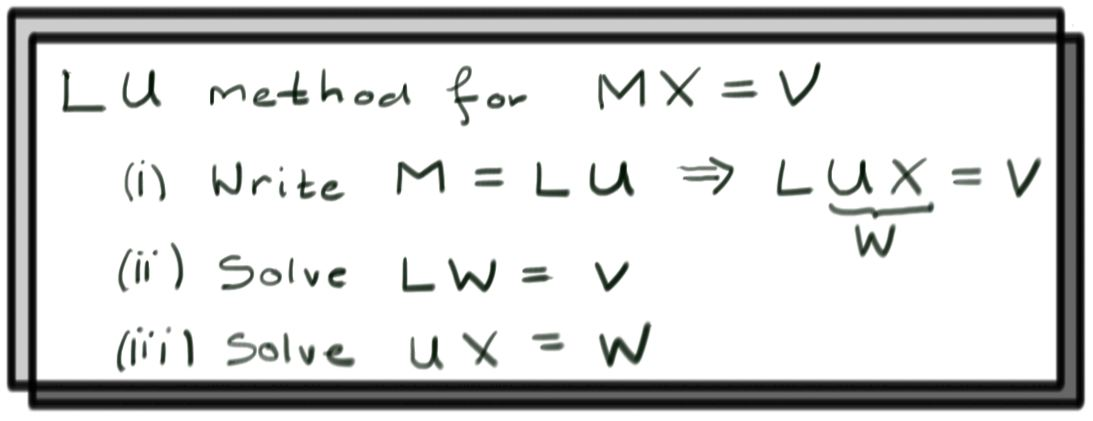
\includegraphics[scale=.3]{\luDecompPath/LU_solution.jpg}
\end{center}
%\end{figure}

\section{Finding an $LU$ Decomposition.}
\label{finding_LU_decomp}
 
For any given matrix, there are actually many different $LU$ decompositions.  However, there is a unique $LU$ decomposition in which the $L$ matrix has ones on the diagonal. In that case $L$ is called a \emph{lower unit triangular matrix}\index{Lower unit triangular matrix}.

To find the $LU$ decomposition, we'll create two sequences of matrices $L_0, L_1, \ldots$ and $U_0, U_1, \ldots$ such that at each step, $L_iU_i=M$.  Each of the $L_i$ will be lower triangular, but only the last $U_i$ will be upper triangular.

Start by setting $L_0=I$ and $U_0=M$, because $L_0U_0=M$. A main concept of this calculation is captured by the following example:

\begin{example}
Consider $$E=\begin{pmatrix}1&0\\\lambda&1\end{pmatrix}\, ,\qquad M=\begin{pmatrix}a&b&c&\cdots\\d&e&f&\cdots\end{pmatrix}\, .$$
Lets compute $EM$
$$
EM=\begin{pmatrix}a&b&c&\cdots\\d+\lambda a&e+\lambda b&f+\lambda c&\cdots\end{pmatrix}\, ,.
$$
Something neat happened here: multiplying $M$ by $E$ performed the row operation $R_2\to R_2+\lambda R-1$ on $M$.
Another interesting fact:
$$
E^{-1}:=\begin{pmatrix}1&0\\-\lambda&1\end{pmatrix}
$$ 
obeys (check this yourself...)
$$
E^{-1} E = 1\, .
$$
Hence $M=E^{-1} E M$ or, writing this out
$$
\begin{pmatrix}a&b&c&\cdots\\d&e&f&\cdots\end{pmatrix}=\begin{pmatrix}1&0\\-\lambda&1\end{pmatrix} \begin{pmatrix}a&b&c&\cdots\\d+\lambda a&e+\lambda b&f+\lambda c&\cdots\end{pmatrix}\, .
$$
Here the matrix on the left is lower triangular, while the matrix on the right has had a row operation performed on it.
\end{example}




\vspace{2mm}
We would like to  use the first row of $U_0$ to zero out the first entry of every row below it.  For our running example, $$U_0=M=\begin{pmatrix}
6 & 18 & 3 \\
2 & 12 & 1 \\
4 & 15 & 3 
\end{pmatrix}\, ,$$ so we would like to perform the row operations $R_2\to R_2 -\frac 13 R_1$ and $R_3\to R_3-\frac 23R_1$.
%so the second row minus $\frac{1}{3}$ of the first row will zero out the first entry in the second row.  Likewise, the third row minus $\frac{2}{3}$ of the first row will zero out the first entry in the third row.
If we perform these row operations on $U_0$ to produce 
$$U_1=\begin{pmatrix}
6 & 18 & 3 \\
0 & 6 & 0 \\
0 & 3 & 1 
\end{pmatrix}\, ,$$
we need to multiply this on the left by a lower triangular matrix $L_1$ so that the product $L_1U_1=M$ still.
The above example shows how to do this:
Set $L_1$ to be the lower triangular matrix whose first column is filled with the minus constants used to zero out the first column of $M$.  Then $$L_1 = \begin{pmatrix}
1 & 0 & 0 \\[1mm]
\frac{1}{3} & 1 & 0 \\[1mm]
\frac{2}{3} & 0 & 1 
\end{pmatrix}\, .$$  
%Set $U_1$ to be the matrix obtained by zeroing out the first column of $M$.  Then $U_1=\begin{pmatrix}
%6 & 18 & 3 \\
%0 & 6 & 0 \\
%0 & 3 & 1 
%\end{pmatrix}$.
By construction $L_1 U_1=M$, but you should compute this yourself as a double check.

Now repeat the process by zeroing the second column of $U_1$ below the diagonal using the second row of $U_1$ using the row operation
$R_3\to R_3-\frac 12 R_2$ to produce
$$U_2=\begin{pmatrix}6&18&3\\0&6&0\\0&0&1\end{pmatrix}\, .$$
The matrix that undoes this row operation is obtained in the same way we found $L_1$ above and is:
$$
\begin{pmatrix}
1&0&0\\
0&1&0\\
0&\frac 12& 0
\end{pmatrix}\, .
$$
Thus our answer for $L_2$ is the product of this matrix with $L_1$, namely
$$
L_2=
\begin{pmatrix}
1 & 0 & 0 \\[1mm]
\frac{1}{3} & 1 & 0 \\[1mm]
\frac{2}{3} & 0 & 1 
\end{pmatrix}\begin{pmatrix}
1&0&0\\
0&1&0\\
0&\frac 12& 0
\end{pmatrix}
=\begin{pmatrix}
1 & 0 & 0 \\[1mm]
\frac{1}{3} & 1 & 0 \\[1mm]
\frac{2}{3} & \frac{1}{2} & 1 
\end{pmatrix}\, .
$$
Notice that it is lower triangular because 

\begin{center}
\textcolor{brown}{THE PRODUCT OF LOWER TRIANGULAR MATRICES IS ALWAYS LOWER TRIANGULAR!}
\end{center}

\noindent
Moreover it is obtained by recording minus the constants used for all our row operations in the appropriate columns (this always works this way).
Moreover, $U_2$ is upper triangular and $M=L_2U_2$, we are done!
Putting this all together we have
$$M=\begin{pmatrix}
6 & 18 & 3 \\
2 & 12 & 1 \\
4 & 15 & 3 
\end{pmatrix}= \begin{pmatrix}
1 & 0 & 0 \\[1mm]
\frac{1}{3} & 1 & 0 \\[1mm]
\frac{2}{3} & \frac{1}{2} & 1 
\end{pmatrix}\begin{pmatrix}
6 & 18 & 3 \\
0 & 6 & 0 \\
0 & 0 & 1 
\end{pmatrix}\, .$$  
%Since $U_2$ is upper-triangular, we're done.  Inserting the new number into $L_1$ to get $L_2$ really is safe: the numbers in the first column don't affect the second column of $U_1$, since the first column of $U_1$ is already zeroed out.

If the matrix you're working with has more than three rows, just continue this process by zeroing out the next column below the diagonal, and repeat until there's nothing left to do.

\videoscriptlink{lu_decomposition_example.mp4}{Another $LU$ decomposition example}{scripts_lu_decomposition_example}

The fractions in the $L$ matrix are admittedly ugly.  For two matrices $LU$, we can multiply one entire column of $L$ by a constant $\lambda$ and divide the corresponding row of $U$ by the same constant without changing the product of the two matrices.  Then:

\begin{eqnarray*}
LU &=& \begin{pmatrix}
1 & 0 & 0 \\[1mm]
\frac{1}{3} & 1 & 0 \\[1mm]
\frac{2}{3} & \frac{1}{2} & 1 
\end{pmatrix}
I
\begin{pmatrix}
6 & 18 & 3 \\
0 & 6 & 0 \\
0 & 0 & 1 
\end{pmatrix} \\
&=&
\begin{pmatrix}
1 & 0 & 0 \\[1mm]
\frac{1}{3} & 1 & 0 \\[1mm]
\frac{2}{3} & \frac{1}{2} & 1 
\end{pmatrix}
\begin{pmatrix}
3 & 0 & 0 \\
0 & 6 & 0 \\
0 & 0 & 1 
\end{pmatrix}
\begin{pmatrix}
\frac{1}{3} & 0 & 0 \\[1mm]
0 & \frac{1}{6} & 0 \\[1mm]
0 & 0 & 1 
\end{pmatrix}
\begin{pmatrix}
6 & 18 & 3 \\
0 & 6 & 0 \\
0 & 0 & 1 
\end{pmatrix} \\
&=&
\begin{pmatrix}
3 & 0 & 0 \\
1 & 6 & 0 \\
2 & 3 & 1 
\end{pmatrix}\begin{pmatrix}
2 & 6 & 1 \\
0 & 1 & 0 \\
0 & 0 & 1 
\end{pmatrix}.
\end{eqnarray*}
The resulting matrix looks nicer, but isn't in standard (lower unit triangular matrix) form.

\reading{11}{2}
%\href{\webworkurl ReadingHomework11/2/}{Reading homework: problem 11.2}

For matrices that are not square, $LU$ decomposition still makes sense.  Given an $m\times n$ matrix $M$, for example we could write $M=LU$ with $L$ a square lower unit triangular matrix, and $U$ a rectangular matrix.  Then $L$ will be an $m\times m$ matrix, and $U$ will be an $m\times n$ matrix (of the same shape as $M$).  From here, the process is exactly the same as for a square matrix.  We create a sequence of matrices $L_i$ and $U_i$ that is eventually the $LU$ decomposition.  Again, we start with $L_0=I$ and $U_0=M$.

\begin{example}
Let's find the $LU$ decomposition of $M=U_0=\begin{pmatrix}
-2 & 1 & 3 \\
-4 & 4 & 1 
\end{pmatrix}$.  Since $M$ is a $2\times 3$ matrix, our decomposition will consist of a $2\times 2$ matrix and a $2\times 3$ matrix.  Then we start with $L_0=I_2=\begin{pmatrix}
1 & 0 \\
0 & 1
\end{pmatrix}$.

The next step is to zero-out the first column of $M$ below the diagonal.  There is only one row to cancel, then, and it can be removed by subtracting $2$ times the first row of $M$ to the second row of $M$.  Then:

\[
L_1=\begin{pmatrix}
1 & 0 \\
2 & 1
\end{pmatrix}, \qquad 
U_1 = \begin{pmatrix}
-2 & 1 & 3 \\
0 & 2 & -5 
\end{pmatrix}
\]
Since $U_1$ is upper triangular, we're done.  With a larger matrix, we would just continue the process.
\end{example}





\section{Block $LDU$ Decomposition}

Let $M$ be a square block matrix with square blocks $X,Y,Z,W$ such that $X^{-1}$ exists.  Then $M$ can be decomposed as a block $LDU$ decomposition, where $D$ is block diagonal, as follows:
\[
M=\begin{pmatrix}
X & Y \\
Z & W
\end{pmatrix}
\]

Then: \[M=\begin{pmatrix}
I &  0 \\
ZX^{-1} & I
\end{pmatrix}\begin{pmatrix}
X & 0 \\
0 & W-ZX^{-1}Y
\end{pmatrix}\begin{pmatrix}
I & X^{-1}Y \\
0 & I
\end{pmatrix}.\]
This can be checked explicitly simply by block-multiplying these three matrices.

\videoscriptlink{lu_decomposition_blocks.mp4}{Block $LDU$ Explanation}{scripts_lu_decomposition_blocks}

\begin{example}
For a $2\times 2$ matrix, we can regard each entry as a block.
\[
\begin{pmatrix}
1 & 2 \\
3 & 4
\end{pmatrix}=
\begin{pmatrix}
1 & 0 \\
3 & 1
\end{pmatrix}
\begin{pmatrix}
1 & 0 \\
0 & -2
\end{pmatrix}
\begin{pmatrix}
1 & 2 \\
0 & 1
\end{pmatrix}
\]
By multiplying the diagonal matrix by the upper triangular matrix, we get the standard $LU$ decomposition of the matrix.
\end{example}


%\section*{References}
%Wikipedia:
%\begin{itemize}
%\item \href{http://en.wikipedia.org/wiki/LU_decomposition}{$LU$ Decomposition}
%\item \href{http://en.wikipedia.org/wiki/Block_LU_decomposition}{Block $LU$ Decomposition}
%\end{itemize}

\section{Review Problems}



\begin{enumerate}

\item Let $D=\begin{pmatrix}
\lambda_1 & \mc0 \\
\mc0 & \lambda_2 \\
\end{pmatrix}$.
\begin{enumerate}
\item Write $D$ in terms of the vectors $e_1$ and $e_2$, and their transposes.
\item Suppose $P=\begin{pmatrix}
a & b \\
c & d \\
\end{pmatrix}$ is invertible.  Show that $D$ is similar to
\[
M=\frac{1}{ad-bc}\begin{pmatrix}
\lambda_1ad-\lambda_2bc & -(\lambda_1-\lambda_2)ab \\[1mm]
(\lambda_1-\lambda_2)cd & -\lambda_1bc + \lambda_2ad
\end{pmatrix}.
\]
\item Suppose the vectors $\rowvec{a,b}$ and $\rowvec{c,d}$ are orthogonal.  What can you say about $M$ in this case? (Hint: think about what \(M^T\) is equal to.)
\end{enumerate}

\phantomnewpage

\item \label{orthogprob} Suppose $S=\{v_1, \ldots, v_n \}$ is an \emph{orthogonal} (not orthonormal) basis for~$\Re^n$.  Then we can write any vector $v$ as $v=\sum_ic^iv_i$ for some constants $c^i$.  Find a formula for the constants $c^i$ in terms of $v$ and the vectors in~$S$.

\Videoscriptlink{orthonormal_bases_hint.mp4}{Hint}{scripts_orthonormal_bases_hint}
\phantomnewpage

\item \label{orthogprojprob} Let $u,v$ be linearly independent vectors in $\Re^3$, and $P=\spa \{ u,v\}$ be the plane spanned by $u$ and $v$.  
\begin{enumerate}
\item Is the vector $v^\bot := v-\frac{u\cdot v}{u\cdot u}u$ in the plane $P$?
\item  What is the (cosine of the) angle between $v^\bot$ and $u$?
\item %Given your solution to the above, 
How can you find a third vector perpendicular to both $u$ and $v^\bot$?
\item  Construct an orthonormal basis for $\Re^3$ from $u$ and $v$.
\item  Test your abstract formul\ae\ starting with 
\[
u=\rowvec{1 , 2 , 0} \text{ and } v=\rowvec{0 , 1 , 1}.
\]
\end{enumerate}

\Videoscriptlink{orthonormal_bases_hint3.mp4}{Hint}{scripts_orthonormal_bases_hint3}

\phantomnewpage



\item Find an orthonormal  basis for $\Re^4$ which includes $(1,1,1,1)$ using the following procedure:\\
\begin{enumerate} 
\item Pick a vector perpendicular to the vector 
$$v_1 =\colvec{1\\1\\1\\1}$$ from the solution set of the matrix equation $$v_1^Tx=0\, .$$ Pick the vector $v_2$ obtained from the standard Gaussian elimination procedure which is the coefficient of $x_2$.
\item Pick a vector perpendicular to both $v_1$ and $v_2$ from the solutions set of the matrix equation $$\colvec{v_1^T\\[1mm]v_2^T}x=0\, .$$ Pick the vector $v_3$ obtained from the standard Gaussian elimination procedure with $x_3$ as the coefficient. 
\item Pick a vector perpendicular to $v_1,v_2,$ and $v_3$ from the solution set of the matrix equation $$\colvec{v_1^T\\[1mm]v_2^T\\[1mm]v_3^T}x=0\, .$$  Pick the vector $v_4$ obtained from the standard Gaussian elimination procedure with $x_3$ as the coefficient. 
\item Normalize the four vectors obtained   above.
\end{enumerate}


\item Use the inner product $$f\cdot g := \int_0^1 f(x)g(x)dx$$  on the vector space $V={\rm span} \{1,x,x^2,x^3\}$ to perform the Gram-Schmidt procedure on the set of vectors $\{1,x,x^2,x^3\}$. 

\item Use the inner product $$f\cdot g := \int_0^{2\pi} f(x)g(x)dx$$  on the vector space $V={\rm span} \{\sin(x),\sin(2x),\sin(3x) \}$ to perform the Gram-Schmidt procedure on the set of vectors $\{\sin(x),\sin(2x),\sin(3x) \}$. \\
Try to build an orthonormal basis for the vector space $$\spa \{ \sin(nx)~| ~n\in \N \}\, .$$
%What do you suspect about the vector space $\spa \{ \sin(nx)~| ~n\in \N \}$?\\
%What do you suspect about the vector space $\spa \{ \sin(ax)~|~ a \in \Re \}$?
\item 
\begin{enumerate}
\item
Show that if $Q$ is an orthogonal $n\times n$ matrix, then $$u\dotprod v = (Qu)\dotprod (Qv)\, ,$$ for any $u,v\in \Re^n$. That is, $Q$ preserves the inner product. 
\item Does $Q$ preserve the outer product? 
\item  If the set of vectors $\{ u_1,\dots,u_n\}$ is orthonormal and $\{ \lambda_1,\cdots,\lambda_n\}$ is a set of numbers, 
then what are the eigenvalues and eigenvectors of the matrix
$M=\sum_{i=1}^n \lambda_i u_i u_i^T$? 
\item How would the eigenvectors and eigenvalues of this matrix change if we replaced  $\{ u_1,\dots,u_n\}$ by $\{ Qu_1,\dots,Q u_n\}$?
\end{enumerate}


\item Carefully write out the Gram-Schmidt procedure for the set of vectors 
$$\left\{ \colvec{1\\1\\1}, \colvec{1\\-1\\1}, \colvec{1\\1\\-1} \right\} \, .$$ Is it possible to rescale the second vector obtained in the procedure to a vector with integer components? 


\item 
\label{basisortho}
\begin{enumerate}
\item Suppose $u$ and $v$ are linearly independent.  Show that $u$ and $v^\perp$ are also linearly independent.  Explain why $\{u, v^\perp\}$ is a basis for $\spa \{u,v\}$.



\Videoscriptlink{gram_schmidt_and_orthogonal_complements_hint.mp4}{Hint}{gram_schmidt_and_orthogonal_complements_hint}

\item Repeat the previous problem, but with three independent vectors $u,v,w$
 where $v^\perp$ and $w^\perp$ are as defined by the Gram-Schmidt procedure. 
\end{enumerate}

\phantomnewpage


\item \label{QRprob} Find the $QR$ factorization of
$$
M=\begin{pmatrix}1&0&\phantom{\!-}2\\-1&2&0\\-1&-2&2
\end{pmatrix}\, .
$$

\phantomnewpage

\item Given any three vectors $u,v,w$, when do $v^\perp$ or $w^\perp$ of the Gram--Schmidt procedure vanish?

\phantomnewpage

\item For $U$ a subspace of $W$, use the subspace theorem to check that $U^\perp$ is a subspace of $W$.

\phantomnewpage


\phantomnewpage

\item %(Extra Credit) 
Let $S_n$ and $A_n$ define the space of $n \times n$ symmetric and anti-symmetric matrices, respectively. These are subspaces of the vector space $M^n_n$ of all $n\times n$ matrices. What is $\dim M^n_n$, $\dim S_n$, and $\dim A_n$? Show that $M^n_n = S_n + A_n$. Define an inner product on square matrices
$$
M\cdot N ={\rm tr} MN\, .
$$
Is $A_n^{\perp}=S_n$? Is $M^n_n = S_n \oplus A_n$?

%\emph{Hint: Note that $\dim S_n = \dim U_n$ where $U_n$ is the vector space of all $n \times n$ upper triangular matrices, and also note that $\dim A_n = \dim \widetilde{U}_n$ where $\widetilde{U}_n$ is the vector space of all strictly $n \times n$ upper triangular matrices (\emph{i.e.} the diagonal entries are all 0).}

\item The vector space $V={\rm span} \{ \sin(t),\sin(2t), \sin(3t) , \sin(3t)\}$ has an inner product: 
$$f\cdot g:=\int _0^{2\pi}f(t)g(t) dt\, .$$ Find the orthogonal compliment to $U={\rm span} \{ \sin(t)+\sin(2t) \}$ in $V$. Express $\sin(t)-\sin(2t)$ as  the sum of vectors from $U$ and $U^\perp$.

\end{enumerate}

\phantomnewpage

\newpage



\appendix


\chapter{List of Symbols}

\begin{center}
\begin{tabular}{ll}
$\in $ & ``Is an element of''.\\[2mm]
\multirow{2}{*}{$\sim$} & ``Is equivalent to'', see \hyperlink{equivalence}{equivalence relations}.\\
&Also, ``is \hyperlink{roweq}{row equivalent} to'' for matrices.\\[2mm]
${\mathbb R}$ & The real numbers.\\[2mm]
$I_n$ & The $n \times n$ identity matrix.\\[2mm]
$P_n^{\mathbb{F}}$ & The vector space of polynomials of degree at most $n$ with \\
 & coefficients in the field $\mathbb{F}$.\\[2mm]
${\mathbb M}_k^r$ & The vector space of $r\times k$ matrices.
\end{tabular}
\end{center}

\newpage


\chapter{Fields}

%\section{Abstract Concepts}
%
%Here we will introduce  some abstract concepts which are mentioned or used in this book. This is material is more advanced but will be interesting to anybody wanting a deeper understanding of the underlying mathematical structures behind linear algebra.  In all cases below, we assume that the given set is closed under the operation(s) introduced.
%
%\subsection{Dual Spaces}
%\label{dualspaces}
%
%\begin{definition}
%\index{Bounded operator}
%A \emph{bounded operator} is a linear operator $\phi \colon V \rightarrow W$ such that $\norm{\phi v}_W \leq C \norm{v}_V$ where $C > 0$ is a fixed constant.
%\end{definition}
%
%Let $V$ be a vector space over $\mathbb{F}$, and a \emph{functional} is a function $\phi \colon V \rightarrow \mathbb{F}$.
%
%\begin{definition}
%\index{Dual space}
%The \emph{dual space} $V^*$ of a vector space $V$ is the vector space of all bounded linear functionals on $V$.
%\end{definition}
%
%There is a natural basis $\{ \Lambda_i \}$ for $V^*$ by $\Lambda_i(e_j) = \delta_{ij}$ where $\{e_j\}$ is the canonical (standard) basis for $V$ and $\delta_{ij}$ is the \emph{Kronecker delta}\index{Kronecker delta}, which is 1 if $i = j$ and 0 otherwise. Concretely for a finite dimensional vector space $V$, we can associate $V^*$ with row vectors $w^T$ as a functional by the matrix multiplication $w^T v$ for vectors $v \in V$. Alternatively we can associated $V^*$ with vectors in $V$ as a functional by taking the usual dot product. So the basis for $V^*$ is $e_i^T$ or $\langle e_i, v \rangle$ for vectors $v \in V$.

%\subsection{Groups}
%\label{groups}
%
%\begin{definition}
%\index{Group}
%A \emph{group} is a set $G$ with a single operation $\cdot$ which satisfies the axioms:
%\begin{itemize}
%\item Associativity $(a \cdot b) \cdot c = a \cdot (b \cdot c)$ for all $a,b,c \in G$.
%
%\item There exists an identity $1 \in G$.
%
%\item There exists an inverse $g^{-1} \in G$ for all $g \in G$.
%\end{itemize}
%\end{definition}
%
%Groups can be finite or infinite, and notice that not alls element in a group must commute ({\it i.e.}, the order of multiplication can matter). Here are some examples of groups:
%\begin{itemize}
%\item Non-zero real numbers under multiplication.
%
%\item All real numbers under addition.
%
%\item All invertible $n \times n$ real matrices.
%
%\item All $n \times n$ real matrices of determinant 1.
%
%\item All permutations of $[1, 2, \dotsc, n]$ \hyperref[problem_permutation]{under compositions}.
%
%\item Any vector space under addition.
%\end{itemize}
%Note that all real numbers under multiplication is not a group since $0$ does not have an inverse.



%\subsection{Fields}
\label{fields}

\begin{definition}
\index{Field}
A \emph{field} $\mathbb{F}$ is a set with two operations $+$ and $\cdot$, such that for all $a, b, c \in \mathbb{F}$  the following axioms are satisfied:
\begin{itemize}
\item[A1.] Addition is associative $(a + b) + c = a + (b + c)$.

\item[A2.] There exists an additive identity $0$.

\item[A3.] Addition is commutative $a + b = b + a$.

\item[A4.] There exists an additive inverse $-a$.

\item[M1.] Multiplication is associative $(a \cdot b) \cdot c = a \cdot (b \cdot c)$.

\item[M2.] There exists a multiplicative identity $1$.

\item[M3.] Multiplication is commutative $a \cdot b = b \cdot a$.

\item[M4.] There exists a multiplicative inverse $a^{-1}$ if $a \neq 0$.

\item[D.] The distributive law holds $a \cdot (b + c) = ab + ac$.
\end{itemize}
\end{definition}
Roughly, all of the above mean that you have notions of $+$, $-$, $\times$ and $\div$ just as for regular real numbers.

Fields are a very beautiful structure; some examples are rational numbers~$\mathbb{Q}$, real numbers $\mathbb{R}$, and complex numbers~$\mathbb{C}$. These examples are infinite, however this does not necessarily have to be the case. 
The smallest example of a field has just two elements, $\mathbb{Z}_2=\{0,1\}$ or {\it bits}. The rules for addition and multiplication 
are the usual ones save that
$$
1+1=0\, .
$$

%Let $q \geq 0$ and let $\mathbb{Z}_q$ be the set of remainders of $\mathbb{Z}$ (the set of integers) by dividing by $q$. We say $\mathbb{Z}_q$ is the set of all $a$ modulo $q$ or $a \mod q$ for short or $a \equiv q$ where $a \in \mathbb{Z}$, and we define addition and multiplication to be their usual counterparts in $\mathbb{Z}$ except we take the result mod $q$. So for example we have $\mathbb{Z}_2 = \{0, 1\}$ where $1 + 1 = 2 \equiv 0$ (these are exactly the \hyperlink{bits}{bits} used in bit matrices) and  $\mathbb{Z}_3 = \{0, 1, 2\}$ with $1 + 1 = 2$, $2 \cdot 2 = 4 \equiv 1$. Now if $p$ is a prime number, then $\mathbb{Z}_p$ is a field (often written as $\mathbb{Z}_p$). Clearly $\mathbb{Z}_2$ is a field, and from above for $\mathbb{Z}_3$ we have $2^{-1} = 2$, so $\mathbb{Z}_3$ is also a field. For $\mathbb{Z}_5$ we have $2^{-1} = 3$ since $2\cdot 3 = 6 \equiv 1$ and $4^{-1} = 4$ since $4 \cdot 4 = 16 \equiv 1$. Often when $q = p^n$ where $p$ is a prime, then people will write $\mathbb{F}_q$ to reinforce that it is a field.

%In fact, for every prime number $p$, the set $\mathbb{Z}_p=\{0,1,\ldots, p-1\} $ forms a field.  The addition and multiplication are obtained by using the usual operations over the integers, and then dividing by $p$ and taking the remainder.  For example, in $\mathbb{Z}_5$, we have $4+3=2$, and $4\cdot4=1$.  (This is sometimes called ``clock arithmetic.'')  Such fields are very important in computer science, cryptography, and number theory.


%\subsection{Rings}
%\label{rings}
%
%However $\mathbb{Z}_4$ is not a field since $2 \cdot 2 = 4 \equiv 0$ and $2 \cdot 3 = 6 \equiv 2$. Similarly $\mathbb{Z}$ is not a field since $2$ does not have a multiplicative inverse.  These are known as \emph{rings}. For rings all of the addition axioms hold, but none of the multiplicative ones must.
%
%\begin{definition}
%\index{Ring}
%A \emph{ring} $R$ is a set with two operations $+$ and $\cdot$ that for all $a, b, c \in R$ the following axioms are satisfied:
%\begin{itemize}
%\item[A1.] Addition is associative $(a + b) + c = a + (b + c)$.
%
%\item[A2.] There exists an additive identity $0$.
%
%\item[A3.] Addition is commutative $a + b = b + a$.
%
%\item[A4.] There exists an additive inverse $-a$.
%
%\item[D.] The distributive law holds $a \cdot (b + c) = a \cdot b + a \cdot c$ and $(a + b) \cdot c = a \cdot c + b \cdot c$.
%\end{itemize}
%\end{definition}
%Note that when we have axiom~M3, then the two equations in axiom~D are equivalent.
%
%Clearly all fields are rings, but rings in general are not nearly as nice (for example, in $\mathbb{Z}_4$ two things can be multiplied together to give you $0$). An important example of a ring is $\mathbb{F}[x]$, which is the ring of all polynomials in one variable $x$ with coefficients in a field $\mathbb{F}$. Recall that you can do everything you want in a field except divide polynomials, but if you take the modulus with respect to a polynomial which is not a product of two smaller polynomials, you can get a field. We call such polynomials \emph{irreducible}. In other words, you take a polynomial $p$ and you set $p \equiv 0$, thus this is just making sure you don't have $ab \equiv 0$. For example, the polynomial $p(x) = x^2 + 1$ cannot be factored over $\mathbb{R}$ (i.e. with real coefficients), so what you get is actually the same field as $\mathbb{C}$ since we have $x^2 + 1 = 0$ or perhaps more suggestively $x^2 = -1$. This is what is known as a \emph{field extension}; these are the central objects in Galois theory\index{Galois} and are denoted $\mathbb{F}(\alpha)$ where $\alpha$ is a root of $p$.
%
%One final definition: We say that a field $\mathbb{F}$ has characteristic $p$ if $\sum_{i=1}^p 1 \equiv 0$ ({\it i.e.} we sum 1 together $p$ times and return to 0). For example $\mathbb{Z}_3$ has characteristic 3 since $1 + 1 + 1 \equiv 0$, and in general $\mathbb{Z}_p$ has characteristic $p$.
%
%A good exercise is to find an irreducible degree 2 polynomial $p$ in $\mathbb{Z}_2[x]$, and check that the field extension $\mathbb{Z}_2(\alpha)$ has 4 elements and has characteristic~2 (hence it is not actually $\mathbb{Z}_4$).
%
%\subsection{Algebras}
%\label{algebras}
%
%\begin{definition}
%\index{Algebra}
%An \emph{algebra} $A$ is a vector space over $\mathbb{F}$ with the operation $\cdot$ such that for all $u, v, w \in A$ and $\alpha, \beta \in \mathbb{F}$, we have
%\begin{itemize}
%\item[D.] The distributive law holds $u \cdot (v + w) = u \cdot v + u \cdot w$ and  $(u + v) \cdot w = u \cdot w + v \cdot w$.
%
%\item[S.] We have $(\alpha v) \cdot (\beta w) = (\alpha \beta)(v \cdot w)$.
%\end{itemize}
%\end{definition}
%Essentially an algebra is a ring that is also a vector space over some field. Or in simpler words,
%an algebra is a vector space where you can multiply vectors.
%
%For example, all $n \times n$ real matrices $M_n(\mathbb{R})$ is a ring but we can let scalars in $\mathbb{R}$ act on these matrices in their usual way. Another algebra is we can take $M_n(\mathbb{R})$ but take scalars in $\mathbb{C}$ and just formally say $i M$ is another element in this algebra. Another example is $\mathbb{R}^3$ where multiplication is the cross-product $\times$. We note that this is not associative nor commutative under $\times$ and that $v \times v = 0$ (so there are in fact no multiplicative inverses), and there is no multiplicative identity. Lastly, recall that $\mathfrak{sl}_n$ \hyperlink{scripts_properties_of_matrices_trace}{defined here} is an algebra under $[ , ]$.

\newpage


\chapter{Online Resources}\label{othersources}

Here are some  internet places to get linear algebra help:

\begin{itemize}
\item
Strang's MIT Linear Algebra Course. Videos of lectures and more:
\URL{http://ocw.mit.edu/courses/mathematics/18-06-linear-algebra-spring-2010/}
\item Beezer's online Linear Algebra Course
\URL{http://linear.ups.edu/version3.html}
\item The Khan Academy has thousands of free videos on a multitude of topics including linear algebra:
\URL{http://www.khanacademy.org/}
\item The Linear Algebra toolkit:
\URLS{http://www.math.odu.edu/~bogacki/lat/}{http://www.math.odu.edu/$\sim$bogacki/lat/}
\item Carter, Tapia and Papakonstantinou's online linear algebra resource
\URL{http://ceee.rice.edu/Books/LA/index.html}
\item
S.O.S. Mathematics Matrix Algebra primer:
\URL{http://www.sosmath.com/matrix/matrix.html}
\item The Numerical Methods Guy on Youtube. Lots of worked examples:
\URL{http://www.youtube.com/user/numericalmethodsguy}
\item Interactive Mathematics. Lots of useful math lessons on many topics:
\URL{http://www.intmath.com/}
\item Stat Trek. A quick matrix tutorial for statistics students:
\URL{http://stattrek.com/matrix-algebra/matrix.aspx}
\item Wolfram's Mathworld. An online mathematics encyclop\ae dia:
\URL{http://mathworld.wolfram.com/}
\item Paul Dawkin's online math notes:
\URL{http://tutorial.math.lamar.edu/}
\item Math Doctor Bob:
\URL{http://www.youtube.com/user/MathDoctorBob?feature=watch}
\item Some pictures of how to rotate objects with matrices:
\URL{http://people.cornellcollege.edu/dsherman/visualize-matrix.html}
\item xkcd. Geek jokes:
\URL{http://xkcd.com/184/}
\item See the bridge actually fall down:
\URL{http://anothermathgeek.hubpages.com/hub/What-the-Heck-are-Eigenvalues-and-Eigenvectors}
\end{itemize}

\newpage

\small

\chapter{Sample First Midterm}

Here are some worked problems typical for what you might expect on a first midterm examination.
\label{sample1}

\begin{enumerate}
\item Solve the following linear system.  Write the solution set in vector form.  Check your solution.  Write one particular solution and one homogeneous solution, if they exist.  What does the solution set look like geometrically?
$$
\begin{array}{rrrrrr}
x &+&3y & &&= 4\\[1mm]
x &-& 2y &+& z &= 1\\[1mm]
2x &+&y &+& z &= 5\\[1mm]
\end{array}
$$

\item
Consider the system of equations
$$
\left\{
\begin{array}{rrrrrrrrr}
x&&&-&z&+&2w&=&-1\\[2mm]
x&+&y&+&z&-&w&=&2\\[2mm]
&-&y&-&2z&+&3w&=&-3\\[2mm]
5x&+&2y&-&z&+&4w&=&1\\[2mm]
\end{array}
\right. 
$$
\begin{enumerate}
\item Write an augmented matrix for this system.
\item Use elementary row operations to find its reduced row echelon form.
\item Write the solution set for the system in the form $$S=\{X_0+\sum_i \mu_i Y_i:\mu_i\in \mathbb R\} .$$
\item What are the vectors $X_0$ and $Y_i$ called {\it and} which matrix equations do they solve?
\item Check separately that $X_0$ and each $Y_i$ solve the matrix systems you claimed they solved in part (d).
\end{enumerate}

\item Use row operations to invert the matrix
$$
\begin{pmatrix}
1&2&3&4\\
2&4&7&11\\
3&7&14&25\\
4&11&25&50
\end{pmatrix}
$$

\item Let $M = \left ( \begin{array}{cc} 2 & 1 \\ 3 & -1 \end{array}  \right )$.  Calculate $M^TM^{-1}$.  Is $M$ symmetric?  What is the trace of the transpose of $f(M)$, where $f(x) = x^2 -1$?

\item In this problem $M$ is the matrix
$$
M=\begin{pmatrix}\cos\theta & \sin\theta \\ -\sin\theta&\cos\theta\end{pmatrix}
$$
and $X$ is the vector
$$
X=\begin{pmatrix}x\\y \end{pmatrix}\, .
$$
Calculate all possible dot products between the vectors $X$ and $MX$. Compute the lengths of $X$ and $MX$.
What is the angle between the vectors $MX$ and $X$. Draw a picture of these vectors in the plane. For what values
of $\theta$ do you expect equality in the triangle and Cauchy--Schwartz inequalities?

\item Let $M$ be the matrix
$$
\begin{pmatrix}
1&0&0&1&0&0\\
0&1&0&0&1&0\\
0&0&1&0&0&1\\
0&0&0&1&0&0\\
0&0&0&0&1&0\\
0&0&0&0&0&1
\end{pmatrix}
$$
Find a formula for $M^k$ for any positive integer power~$k$. Try some simple examples like $k=2,3$ if confused.



\item What does it mean for a function to be linear?  Check that integration is a linear function from $V$ to $V$, where $V = \{ f: \mathbb{R} \to \mathbb{R} \mid f \textrm{ is integrable}\}$ is a vector space over $\mathbb{R}$ with usual addition and scalar multiplication.


\item What are the four main things we need to define for a vector space?  Which of the following is a vector space over $\mathbb{R}$?  For those that are not vector spaces, modify one part of the definition to make it into a vector space.
\begin{enumerate}
\item $V = \{ \textrm{ $2 \times 2$ matrices with entries in $\mathbb{R}$} \}$, usual matrix addition, and $k \cdot \left ( \begin{array}{cc} a & b \\ c & d \end{array}  \right ) = \left ( \begin{array}{cc} ka & b \\ kc & d \end{array}  \right )$ for $k \in \mathbb{R}$.

\item $V = \{ \textrm{polynomials with complex coefficients of degree $\leq 3$} \}$, with usual addition and scalar multiplication of polynomials.

\item $V = \{ \textrm{vectors in $\mathbb{R}^3$ with at least one entry containing a 1}\}$, with usual addition and scalar multiplication.
\end{enumerate}


\item
{\it Subspaces:} If $V$ is a vector space, we say that $U$ is a {\it subspace} of $V$ when the set $U$ is also a vector space,
using the vector addition and scalar multiplication rules of the vector space $V$. 
(Remember that $U\subset V$  says that  ``$U$ is a subset of $V$'', {\it i.e.}, all elements of $U$
are also elements of $V$. The symbol $\forall$ means ``for all'' and $\in$ means ``is an element of''.)

\noindent
Explain why additive closure ($u+w\in U$ $\forall$ $u,v\in U$) and multiplicative closure ($r.u\in U$ $\forall$ $r\in \mathbb R$, $u\in V$) 
ensure that (i) the zero vector $0\in U$ and (ii) every $u\in U$ has an additive inverse.\\[2mm]

\noindent
In fact it suffices to check closure under addition and scalar multiplication to verify that $U$ is a vector space. Check whether the following
choices of $U$ are vector spaces:
\begin{enumerate}
\item
$U=\left\{\begin{pmatrix}x\\y\\0\end{pmatrix}:x,y\in \mathbb R\right\}$
\item
$U=\left\{\begin{pmatrix}1\\0\\z\end{pmatrix}:z\in \mathbb R\right\}$
\end{enumerate}

\item
Find an LU decomposition for the matrix 
$$
\begin{pmatrix}
1&1&-1&2\\
1&3&2&2\\
-1&-3&-4&6\\
0&4&7&-2
\end{pmatrix}
$$
Use your result to solve the system
$$
\left\{
\begin{array}{cccccccc}
x&+&y&-&z&+&2w&=7\\[1mm]
x&+&3y&+&2z&+&2w&=6\\[1mm]
-x&-&3y&-&4z&+&6w&=12\\[1mm]
&&4y&+&7z&-&2w&=-7
\end{array}
\right.
$$

\end{enumerate}

\subsection*{Solutions}

\begin{enumerate}
\item
{\it As an additional exercise, write out the row operations above the $\sim$ signs below.}
$$
\left(\begin{array}{rrr|r}
1&3&0&4\\[1mm]1&-2&1&1\\[1mm]2&1&1&5
\end{array}\right)
\sim
\left(\begin{array}{rrr|r}
1&3&0&4\\[1mm]0&-5&1&-3\\[1mm]0&-5&1&-3
\end{array}\right)
\sim
\left(\begin{array}{rrr|r}
1&0&\frac35&\frac{11}{5}\\[1mm]0&1&-\frac15&\frac35\\[1mm]0&0&0&0
\end{array}\right).
$$
Solution set is 
$$
\left\{\begin{pmatrix}x\\y\\ z\end{pmatrix}=\begin{pmatrix}\frac{11}5\\[1mm] \frac35\\ 0\end{pmatrix}+\mu
\begin{pmatrix}-\frac35\\\frac15\\1\end{pmatrix}\colon \mu \in \mathbb{R}
\right\}.
$$
Geometrically this represents a line in ${\mathbb R}^3$ through the point 
$\begin{pmatrix}\frac{11}5\\[1mm] \frac35\\ 0\end{pmatrix}$ 
running parallel to the vector 
$\begin{pmatrix}-\frac35\\[1mm]\frac15\\[1mm]1\end{pmatrix}$.

The vector 
$\ccolvec{\frac{11}5\\[1mm] \frac35\\ 0}$ 
is {\it a} particular solution 
and $\begin{pmatrix}-\frac35\\\frac15\\1\end{pmatrix}$
is {\it a} homogeneous solution. 

As a double check note that 
$$
\left(\begin{array}{rrr}
1&3&0\\1&-2&1\\2&1&1
\end{array}\right)\  \begin{pmatrix}\frac{11}5\\ \frac35\\ 0\end{pmatrix}=\begin{pmatrix}4\\ 1\\ 5\end{pmatrix}
\mbox{ and }
\left(\begin{array}{rrr}
1&3&0\\1&-2&1\\2&1&1
\end{array}\right)\ \begin{pmatrix}-\frac35\\\frac15\\1\end{pmatrix}=\begin{pmatrix}0\\0\\0\end{pmatrix}\, .
$$


\item

\begin{enumerate}
\item The augmented matrix 
$$
\left(\begin{array}{rrrr|r}
1&0&-1&2&-1\\[1mm]
1&1&1&-1&2\\[1mm]
0&-1&-2&3&-3\\[1mm]
5&2&-1&4&1
\end{array}\right)
$$
encodes the system of equations. 
\item 
{\it Again, write out the row operations as an additional exercise.}\\
The above augmented matrix is row equivalent to  
$$
%\sim
\left(\begin{array}{rrrr|r}
1&0&-1&2&-1\\[1mm]
0&1&2&-3&3\\[1mm]
0&-1&-2&3&-3\\[1mm]
0&2&4&-6&6
\end{array}\right)
\sim
\left(\begin{array}{rrrr|r}
1&0&-1&2&-1\\[1mm]
0&1&2&-3&3\\[1mm]
0&0&0&0&0\\[1mm]
0&0&0&0&0
\end{array}\right)
$$
which is in reduced row echelon form.

\item
Solution set is 
$$
\left\{X=\begin{pmatrix}-1\\3 \\ 0\\0\end{pmatrix}
+\mu_1 \begin{pmatrix} 1 \\-2\\1\\0\end{pmatrix}
+\mu_2 \begin{pmatrix}-2\\3\\0\\1\end{pmatrix}
\colon \mu_1,\mu_2 \in \mathbb{R}
\right\}\, .
$$

\item
The vector $X_0=\begin{pmatrix}-1\\3 \\ 0\\0\end{pmatrix}$ is {\it a } particular solution and the vectors 
$$Y_1=\begin{pmatrix} 1 \\-2\\1\\0\end{pmatrix} 
{\rm ~and~ } 
Y_2= \begin{pmatrix}-2\\3\\0\\1\end{pmatrix}$$ 
are homogeneous solutions.
They obey
$$
MX=V\, ,\qquad M Y_1=0=MY_2\, .
$$
where 
$$M=\left(\begin{array}{rrrr}
1&0&-1&2\\
1&1&1&-1\\
0&-1&-2&3\\
5&2&-1&4
\end{array}\right) {\rm ~and~}
V=\begin{pmatrix}-1\\2\\-3\\1\end{pmatrix}.$$ 

\item This amounts to  explicitly performing the matrix manipulations 
$$MX-V,~ MY_1, {\rm ~and~} MY_2$$
to verify that they are all zero vectors.

\end{enumerate}

\item 
{\it As usual, be sure to write out the row operations above the $\sim$'s so your work can be easily checked.}
$$
\phantom{\sim}
\left(
\begin{array}{rrrr|rrrr}
1&2&3&4&1&0&0&0\\
2&4&7&11&0&1&0&0\\
3&7&14&25&0&0&1&0\\
4&11&25&50&0&0&0&1
\end{array}\right)
$$
$$
\sim
\left(
\begin{array}{rrrr|rrrr}
1&2&3&4&1&0&0&0\\
0&0&1&3&-2&1&0&0\\
0&1&5&13&-3&0&1&0\\
0&3&13&34&-4&0&0&1
\end{array}\right)
$$
$$
\sim
\left(
\begin{array}{rrrr|rrrr}
1&0&-7&-22&7&0&-2&0\\
0&1&5&13&-3&0&1&0\\
0&0&1&3&-2&1&0&0\\
0&0&-2&-5&5&0&-3&1
\end{array}\right)
$$
$$
\sim
\left(
\begin{array}{rrrr|rrrr}
1&0&0&-1&-7&7&-2&0\\
0&1&0&-2&7&-5&1&0\\
0&0&1&3&-2&1&0&0\\
0&0&0&1&1&2&-3&1
\end{array}\right)
$$
$$
\sim
\left(
\begin{array}{rrrr|rrrr}
1&0&0&0&-6&9&-5&1\\
0&1&0&0&9&-1&-5&2\\
0&0&1&0&-5&-5&9&-3\\
0&0&0&1&1&2&-3&1
\end{array}\right)\, .
$$
Check
$$
\begin{pmatrix}
1&2&3&4\\2&4&7&11\\3&7&14&25\\4&11&25&50
\end{pmatrix}
\begin{pmatrix}
-6&9&-5&1\\9&-1&-5&2\\-5&-5&9&-3\\1&2&-3&1
\end{pmatrix}
=
\begin{pmatrix}
1&0&0&0\\0&1&0&0\\0&0&1&0\\0&0&0&1
\end{pmatrix}\, .
$$

\item
$$
M^T M^{-1}=
\begin{pmatrix}2&3\\1&-1\end{pmatrix}\begin{pmatrix}\frac15&\frac15\\[1mm]\frac35&-\frac25\end{pmatrix}
=\begin{pmatrix}\frac{11}5&-\frac45\\-\frac25&\frac35\end{pmatrix}\, .
$$
Since $M^TM^{-1}\neq I$, it follows $M^T\neq M$ so $M$ is {\it not} symmetric.
Finally
$$
{\rm tr} f(M)^T= {\rm tr} f(M) = {\rm tr}(M^2-I)={\rm tr}\begin{pmatrix}2&1\\3&-1\end{pmatrix}\begin{pmatrix}2&1\\3&-1\end{pmatrix}-{\rm tr} I
$$
$$
=(2\cdot 2+1\cdot 3)+(3\cdot 1+(-1)\cdot(-1))-2=9\, .
$$

\item First $$X\dotprod (MX)=X^T M X = \begin{pmatrix}x & y\end{pmatrix}
\begin{pmatrix}\cos\theta &\sin\theta \\ -\sin\theta & \cos\theta\end{pmatrix}
\begin{pmatrix}x \\ y\end{pmatrix}$$
$$
\hspace{2cm}
= \begin{pmatrix}x & y\end{pmatrix}\begin{pmatrix}x \cos\theta + y\sin\theta \\ -x\sin\theta + y\cos\theta\end{pmatrix}
=(x^2+y^2)\cos\theta\, .
$$
Now $||X||=\sqrt{X\dotprod X}=\sqrt{x^2 + y^2}$ and 
$
(MX)\dotprod (MX)= X M^T M X
$. But
$$
M^T M = \begin{pmatrix}\cos\theta &-\sin\theta \\ \sin\theta & \cos\theta\end{pmatrix}
\begin{pmatrix}\cos\theta &\sin\theta \\ -\sin\theta & \cos\theta\end{pmatrix}$$ $$=
\begin{pmatrix}\cos^2\theta +\sin^2\theta& 0 \\ 0 & \cos^2\theta +\sin^2\theta\end{pmatrix}=I\, .
$$
Hence $||MX||=||X||=\sqrt{x^2+y^2}$. Thus the cosine of the angle between $X$ and $MX$ is given by
$$
\frac{X\dotprod (MX)}{||X|| \ ||MX||}= \frac{(x^2+y^2)\cos\theta}{\sqrt{x^2+y^2}\, \sqrt{x^2+y^2}} = \cos \theta\, .
$$
In other words, the angle is $\theta$ OR $-\theta$. You should draw two pictures, one where the angle between
$X$ and $MX$ is $\theta$, the other where it is $-\theta$. 


For Cauchy--Schwartz, $\frac{|X\dotprod (MX)|}{||X|| \ ||MX||}=|\cos\theta|=1$ when $\theta=0,\pi$. 
For the triangle equality $MX = X$ achieves $||X+MX||=||X||+||MX||$, which requires $\theta=0$. 

\item This is a block matrix problem. Notice the that matrix $M$ is really just $M=
\begin{pmatrix}
I&I\\0&I
\end{pmatrix}
$, where $I$ and $0$ are the $3\times3$ identity zero matrices, respectively. But
$$
M^2=\begin{pmatrix}
I&I\\0&I
\end{pmatrix}
\begin{pmatrix}
I&I\\0&I
\end{pmatrix}
=
\begin{pmatrix}
I&2I\\0&I
\end{pmatrix}
$$
and 
$$
M^3=\begin{pmatrix}
I&I\\0&I
\end{pmatrix}
\begin{pmatrix}
I&2I\\0&I
\end{pmatrix}
=
\begin{pmatrix}
I&3I\\0&I
\end{pmatrix}
$$
so, $M^k=\begin{pmatrix}
I&kI\\0&I
\end{pmatrix}$, or explicitly
$$
M^k=
\begin{pmatrix}
1&0&0&k&0&0\\
0&1&0&0&k&0\\
0&0&1&0&0&k\\
0&0&0&1&0&0\\
0&0&0&0&1&0\\
0&0&0&0&0&1
\end{pmatrix}\, .
$$


\item We can call a function $f\colon V\longrightarrow W$ {\it linear} if the sets $V$ and $W$ are vector spaces
and $f$ obeys
$$
f(\alpha u + \beta v)=\alpha f(u)+\beta f(v)\, ,
$$
for all $u,v\in V$ and $\alpha,\beta\in {\mathbb R}$.

Now, integration is a linear transformation from 
the space $V$ of all integrable functions (don't be confused between the definition of a linear function above, 
and integrable functions $f(x)$ which here are the vectors in $V$) to the real numbers ${\mathbb R}$, because 
$\int_{-\infty}^\infty (\alpha f(x) +\beta g(x))dx = \alpha \int_{-\infty}^\infty f(x) dx + \beta \int_{-\infty}^\infty g(x) dx$.

\item The four main ingredients are
(i) a set $V$ of vectors, (ii) a number field~$K$ (usually $K={\mathbb R})$, (iii) a rule for adding vectors (vector addition) and (iv) a way to multiply vectors by a number to produce a new vector (scalar multiplication). 
There are, of course, \hyperref[vectorspace]{ten rules} that these four ingredients must obey.

\begin{enumerate}
\item This is not a vector space. Notice that distributivity of scalar multiplication requires
$2 u = (1+1) u = u + u$ for any vector $u$ but
$$
2\cdot \begin{pmatrix} a& b\\ c& d\end{pmatrix} =  \begin{pmatrix} 2a& b\\ 2c& d\end{pmatrix}
$$
which does {\it not} equal
$$
\begin{pmatrix} a& b\\ c& d\end{pmatrix}+\begin{pmatrix} a& b\\ c& d\end{pmatrix}=
\begin{pmatrix} 2a& 2b\\ 2c& 2d\end{pmatrix}\, .
$$ 
This could be repaired by taking $$ k\cdot \begin{pmatrix} a& b\\ c& d\end{pmatrix}=
\begin{pmatrix} ka& kb\\ kc& kd\end{pmatrix}\, .$$
\item This is a vector space. {\it Although, the question does not ask you to, it is a useful exercise
to verify that all \hyperref[vectorspace]{ten vector space rules} are satisfied.}
\item This is not a vector space for many reasons. An easy one is that $(1,-1,0)$ and $(-1,1,0)$
are both in the space, but their sum $(0,0,0)$ is not ({\it i.e.}, additive closure fails).
The easiest way to repair this would be to drop the requirement that there be at least one entry equaling 1.
 
 \end{enumerate}
 
 \item 
 (i) Thanks to multiplicative closure, if $u\in U$, so is $(-1)\cdot u$. But $(-1) \cdot u + u = (-1)\cdot u + 1\cdot u
 = (-1+1)\cdot u= 0.u = 0$ (at each step in this chain of equalities we have used the fact that $V$ is a vector space
 and therefore can use its vector space rules). In particular, this means that the zero vector of $V$ is in $U$ and  is its
 zero vector also.  (ii) Also, in $V$, for each $u$ there is an element $-u$ such that $u+(-u)=0$. But by additive 
 close, $(-u)$ must also be in $U$, thus every $u\in U$ has an additive inverse.
 
 
 \begin{enumerate}
 \item This is a vector space. First we check additive closure: let $\begin{pmatrix}x \\ y\\0\end{pmatrix}$ and $\begin{pmatrix}z \\ w\\0\end{pmatrix}$
 be arbitrary vectors in $U$. But since $\begin{pmatrix}x \\ y\\0\end{pmatrix} + \begin{pmatrix}z \\ w\\0\end{pmatrix}
 = \begin{pmatrix}x+z \\ y+w\\0\end{pmatrix}$, so is their sum (because vectors in $U$ are those whose third component vanishes).  Multiplicative closure is similar: for any $\alpha\in {\mathbb R}$, $\alpha \begin{pmatrix}x \\ y\\0\end{pmatrix}= \begin{pmatrix}\alpha x \\ \alpha y\\0\end{pmatrix}$, which also has no third component, so is in $U$.
 
 \item This is not a vector space for various reasons. A simple one is that $u=\begin{pmatrix}1\\0\\z\end{pmatrix}$
 is in~$U$ but the vector $u+u=\begin{pmatrix}2\\0\\2z\end{pmatrix}$ is not in~$U$ (it has a 2 in the first component, 
 but vectors in~$U$ always have a 1 there).
 \end{enumerate}
 

\item
$$
\begin{pmatrix}
1&1&-1&2\\
1&3&2&2\\
-1&-3&-4&6\\
0&4&7&-2
\end{pmatrix}
=
\begin{pmatrix}
1&0&0&0\\
1&1&0&0\\
-1&0&1&0\\
0&0&0&1
\end{pmatrix}
\begin{pmatrix}
1&1&-1&2\\
0&2&3&0\\
0&-2&-5&8\\
0&4&7&-2
\end{pmatrix}
$$
$$
=
\begin{pmatrix}
1&0&0&0\\
1&1&0&0\\
-1&-1&1&0\\
0&2&0&1
\end{pmatrix}
\begin{pmatrix}
1&1&-1&2\\
0&2&3&0\\
0&0&-2&8\\
0&0&1&-2
\end{pmatrix}
$$ $$=
\begin{pmatrix}
1&0&0&0\\
1&1&0&0\\
-1&-1&1&0\\
0&2&-\frac12&1
\end{pmatrix}
\begin{pmatrix}
1&1&-1&2\\
0&2&3&0\\
0&0&-2&8\\
0&0&0&2
\end{pmatrix}\, .
$$
To solve $MX=V$ using $M=LU$ we first solve $LW=V$ whose augmented matrix reads
$$
\left(
\begin{array}{cccc|c}
1&0&0&0&7\\
1&1&0&0&6\\
-1&-1&1&0&12\\
0&2&-\frac12&1&-7
\end{array}\right)
\sim 
\left(
\begin{array}{cccc|c}
1&0&0&0&7\\
0&1&0&0&-1\\
0&0&1&0&18\\
0&2&-\frac12&1&-7
\end{array}\right)$$ $$\sim 
\left(
\begin{array}{cccc|c}
1&0&0&0&7\\
0&1&0&0&-1\\
0&0&1&0&18\\
0&0&0&1&4
\end{array}\right)\, ,
$$
from which we can read off $W$.
Now we compute $X$ by solving $UX=W$ with the augmented matrix
$$
\left(
\begin{array}{cccc|c}
1&1&-1&2&7\\
0&2&3&0&-1\\
0&0&-2&8&18\\
0&0&0&2&4
\end{array}\right)
\sim
\left(
\begin{array}{cccc|c}
1&1&-1&2&7\\
0&2&3&0&-1\\
0&0&-2&0&2\\
0&0&0&1&2
\end{array}\right)
$$
$$
\sim
\left(
\begin{array}{cccc|c}
1&1&-1&2&7\\
0&2&0&0&2\\
0&0&1&0&-1\\
0&0&0&1&2
\end{array}\right)
\sim
\left(
\begin{array}{cccc|c}
1&0&0&0&1\\
0&1&0&0&1\\
0&0&1&0&-1\\
0&0&0&1&2
\end{array}\right).
$$
So $x=1$, $y=1$, $z=-1$ and $w=2$.

\end{enumerate}

\newpage

%
\chapter{Sample Second Midterm}

Here are some worked problems typical for what you might expect on a second midterm examination.
\label{sample2}

\begin{enumerate}

\item
{\it Determinants:} The determinant ${\rm det}\, M$ of a $2\times 2$ matrix $M=\begin{pmatrix}a&b\\c&d\end{pmatrix}$ is defined~by
$$
{\rm det}\,  M =ad -bc\, .
$$ 
\begin{enumerate}
\item For which values of ${\rm det}\,  M$ does $M$ have an inverse?
\item Write down all $2\times 2$ bit matrices with determinant~1. (Remember bits are either 0 or 1 and $1+1=0$.)
\item Write down all $2\times 2$ bit matrices with determinant~0.
\item Use one of the above examples to show why the following statement is FALSE.
\begin{quote}
{\it Square matrices with the same determinant are always row equivalent.}
\end{quote}
\end{enumerate}



\item
Let 
$$
A=\left(\begin{array}{ccc}1&1&1\\[2mm]2&2&3\\[2mm]4&5&6\end{array}\right)\, .
$$
Compute $\det A$.
Find all solutions to (i) $A X =  0$ and (ii) $A X=\left(
\begin{array}{c}1\\2\\3\end{array}\right)$ for the vector $X\in \mathbb R^3$. Find, but do not solve,
the characteristic polynomial of $A$.

\item
Let $M$ be any $2\times 2$ matrix. Show
$$
\det M = -\frac 12 {\rm tr} M^2 + \frac 12 ({\rm tr} M)^2\, .
$$

\item
{\it The permanent:} Let $M=(M^i_j)$ be an $n\times n$ matrix. An operation producing a single number from $M$ similar
to the determinant is the ``permanent''
$$
{\rm perm} \, M =\sum_\sigma M^1_{\sigma(1)} M^2_{\sigma(2)}\cdots M^n_{\sigma(n)}\, .
$$
For example
$$
{\rm perm} \begin{pmatrix}a & b \\ c & d\end{pmatrix}=ad+bc\, .
$$
{Calculate} 
$$
{\rm perm} \begin{pmatrix}1 & 2 & 3 \\ 4 & 5 & 6 \\ 7 & 8 & 9\end{pmatrix}\, .
$$
\noindent
What do you think would happen to the permanent of an $n\times n$ matrix~$M$ if (include a {\it brief} explanation with each answer):
\begin{enumerate}
\item You multiplied $M$ by a number $\lambda$.
\item You multiplied a row of $M$ by a number $\lambda$.
\item You took the transpose of $M$.
\item  You swapped two rows of $M$.
\end{enumerate}


\item
Let $X$ be an $n\times 1$ matrix subject to
$$
{X}^{T} X=(1)\, ,
$$
and define
$$
H=I - 2 X \,\!X^T\, ,
$$
(where $I$ is the $n\times n$ identity matrix).
Show 
$$
H=H^{T}=H^{-1}.
$$

\item Suppose $\lambda$ is an eigenvalue of the matrix $M$ with associated eigenvector~$v$.
Is~$v$ an eigenvector of $M^k$ (where $k$ is any positive integer)? If so, what would the associated
eigenvalue be?

Now suppose that the matrix $N$ is {\it nilpotent}, {\it i.e.}
$$
N^k=0
$$
for some integer $k\geq 2$. Show that 0 is the only eigenvalue of $N$.

\item
Let $M=\begin{pmatrix}3&-5\\[2mm]1&-3\end{pmatrix}$. Compute $M^{12}$. (Hint: $2^{12}=4096$.)

\item {\it The Cayley Hamilton Theorem}:
Calculate the characteristic polynomial $P_M(\lambda)$ of the matrix $M=\begin{pmatrix}a & b\\c & d\end{pmatrix}$.
Now compute the matrix polynomial $P_M(M)$. What do you observe? Now suppose the $n\times n$ matrix $A$
is ``similar'' to a diagonal matrix $D$, in other words $$A=P^{-1}DP$$ for some invertible matrix $P$ and $D$ is a matrix with values $\lambda_1$, $\lambda_2,\ldots \lambda_n$ along its diagonal. Show that the two matrix polynomials $P_A(A)$ and $P_A(D)$ are similar ({\it i.e.} $P_A(A)=P^{-1} P_A(D) P$).
Finally, compute $P_A(D)$, what can you say about $P_A(A)$?

\item
{\it Define} what it means for a set $U$ to be a subspace of a vector space $V$.
Now let $U$ and $W$ be non-trivial subspaces of $V$. Are the following also subspaces? (Remember that $\cup$ means ``union'' and $\cap$ means ``intersection''.)
\begin{enumerate}
\item $U \cup  W$
\item $U \cap W$ 
\end{enumerate}
In each case {\it draw} examples in $\mathbb R^3$ that justify your answers. If you answered ``yes'' to either part also give a general 
explanation why this is the case.

\item
{\it Define} what it means for a set of vectors $\{v_1,v_2,\ldots,v_n\}$ to (i) be linearly independent, (ii)
  span a vector space~$V$ and (iii)
 be a basis for a vector space~$V$.

Consider the following vectors in $\mathbb R^3$
$$ u =\begin{pmatrix} -1\\ -4\\ 3 \end{pmatrix}\, ,\qquad
     v =\begin{pmatrix} 4\\ 5\\ 0 \end{pmatrix}\, ,\qquad
    w =\begin{pmatrix} 10\\ 7\\ h+3 \end{pmatrix}\, .
$$
For which values of $h$ is $\{u,v,w\}$ a basis for $\mathbb R^3$?



 \end{enumerate}

\subsection*{Solutions}

\begin{enumerate}
\item 
\begin{enumerate}
\item Whenever ${\rm det} M=ad-bc\neq 0$.
\item Unit determinant bit matrices:
$$
\begin{pmatrix}
1&0\\0&1
\end{pmatrix},
\begin{pmatrix}
1&1\\0&1
\end{pmatrix}\, ,
\begin{pmatrix}
1&0\\1&1
\end{pmatrix},
\begin{pmatrix}
0&1\\1&0
\end{pmatrix}\, ,
\begin{pmatrix}
1&1\\1&0
\end{pmatrix},
\begin{pmatrix}
0&1\\1&1
\end{pmatrix}\,.
$$
\item Bit matrices with vanishing determinant:
$$
\begin{pmatrix}
0&0\\0&0
\end{pmatrix},
\begin{pmatrix}
1&0\\0&0
\end{pmatrix}\, ,
\begin{pmatrix}
0&1\\0&0
\end{pmatrix}\, ,
\begin{pmatrix}
0&0\\1&0
\end{pmatrix},
\begin{pmatrix}
0&0\\0&1
\end{pmatrix}\, ,$$ $$
\begin{pmatrix}
1&1\\0&0
\end{pmatrix},
\begin{pmatrix}
0&0\\1&1
\end{pmatrix}\,,
\begin{pmatrix}
1&0\\1&0
\end{pmatrix},
\begin{pmatrix}
0&1\\0&1
\end{pmatrix}\, ,
\begin{pmatrix}
1&1\\1&1
\end{pmatrix}\,.
$$
{\it As a check, count that the total number of $2\times 2$ bit matrices is $2^{(\rm number\  of\  entries)}=2^4=16$.}
\item To disprove this statement, we just need to find a single counterexample. 
All the unit determinant examples above  are actually row equivalent to the identity matrix, so focus on 
the bit matrices with vanishing determinant. Then notice (for example), that
$$
\begin{pmatrix}
1&1\\0&0
\end{pmatrix}{\sim}\!\!\!\!/
\begin{pmatrix}
0&0\\0&0
\end{pmatrix}\, .
$$ 
So we have found a pair of matrices that are not row equivalent but do have the same determinant. 
It follows that the statement is false.
\end{enumerate}




\item
$$
{\rm det }A= 1.(2.6-3.5)-1.(2.6-3.4)+1.(2.5-2.4)=-1\, .
$$
(i) Since ${\rm det}A\neq 0$, the homogeneous system $AX=0$ only has the solution $X=0$.
(ii) It is efficient to compute the adjoint
$$
{\rm adj}\ A= \begin{pmatrix}-3&0& 2\\ -1&2& -1 \\1&-1 & 0 \end{pmatrix}^{\!T}
= \begin{pmatrix}-3&-1& 1\\ 0&2& -1 \\2&-1 & 0 \end{pmatrix}
$$
Hence
$$A^{-1}=\begin{pmatrix}3&1& -1\\ 0&-2& 1 \\-2&1 & 0 \end{pmatrix}\, .$$

Thus
$$
X=\begin{pmatrix}3&1& -1\\ 0&-2& 1 \\-2&1 & 0 \end{pmatrix}
\begin{pmatrix}1\\2\\3
\end{pmatrix}=
\begin{pmatrix}2\\-1\\0
\end{pmatrix}\, .
$$
Finally, 
$$
P_A(\lambda)=-\det \begin{pmatrix}1-\lambda&1&1\\2&2-\lambda&3\\4&5&6-\lambda\end{pmatrix}$$
$$
=-\Big[(1-\lambda)[(2-\lambda)(6-\lambda)-15]-[2.(6-\lambda)-12]+[10-4.(2-\lambda)]\Big]
$$
$$
=\lambda^3-9\lambda^2-\lambda+1\, .
$$
\item
Call $M=\begin{pmatrix}a&b\\c&d\end{pmatrix}$. Then ${\rm det} M= ad-bc$, yet
$$
-\frac 12 \tr M^2 + \frac12 (\tr M)^2 = -\frac 12 \tr \begin{pmatrix}a^2 + bc & * \\ * & bc + d^2\end{pmatrix} -\frac12 (a+d)^2$$ $$ 
=-\frac 12 (a^2 + 2bc + d^2) + \frac 12 (a^2 + 2ad + d^2) = ad - bc\, ,
$$
which is what we were asked to show.

\item 

$$
{\rm perm} \begin{pmatrix}1 & 2 & 3 \\ 4 & 5 & 6 \\ 7 & 8 & 9\end{pmatrix}
=1\cdot(5\cdot9+6\cdot8)+2\cdot(4\cdot9+6\cdot7)+3\cdot(4\cdot8+5\cdot7)=450\, .
$$

\begin{enumerate}
\item Multiplying $M$ by $\lambda$ replaces every matrix element $M^i_{\sigma(j)}$ in the formula for the permanent
by $\lambda M^i_{\sigma(j)}$, and therefore produces an overall factor $\lambda^n$.
\item Multiplying the $i^{\rm th}$ row by $\lambda$ replaces $M^i_{\sigma(j)}$ in the formula for the permanent
by $\lambda M^i_{\sigma(j)}$. Therefore the permanent is multiplied by an overall factor $\lambda$.
\item The permanent of a matrix transposed equals the permanent of the original matrix, because
in the formula for the permanent this amounts to summing over permutations of rows rather than columns. But we could
then sort the product $M^{\sigma(1)}_1 M^{\sigma(2)}_2\ldots M^{\sigma(n)}_n$ back into its original order using the inverse permutation
 $\sigma^{-1}$. But summing over permutations is equivalent to summing over inverse permutations, and therefore the permanent is unchanged.
\item Swapping two rows also leaves the permanent unchanged. The argument is almost the same as in the previous part, except 
that we need only reshuffle two matrix elements $M^j_{\sigma(i)}$ and $M^i_{\sigma(j)}$ (in the case where rows $i$ and $j$ were swapped).
Then we use the fact that summing over all permutations $\sigma$ or over all permutations $\widetilde \sigma$ obtained
by swapping a pair in $\sigma$ are equivalent operations.
\end{enumerate}

\item Firstly, lets call $(1)=1$ (the $1\times 1$ identity matrix). Then we calculate
$$
H^T=(I-2 X X^T)^T = I^T -2 (X X^T)^T = I -2 (X^T)^T X^T = I - 2 X X^T = H\, ,
$$
which demonstrates the first equality. Now we compute
$$
H^2 = (I-2 X X^T) (I - 2 X X^T) = I - 4 X X^T + 4 X X^T X X^T $$ $$= I - 4 X X^T + 4 X (X^T X) X^T = I - 4 X X^T + 4 X.  1  .X^T = I\, .
$$
So, since $HH=I$, we have $H^{-1}=H$.

\item We know $Mv=\lambda v$. Hence 
$$
M^2 v = M M v = M \lambda v = \lambda M v = \lambda^2 v\, , 
$$
and similarly
$$
M^k v = \lambda M^{k-1} v = \ldots = \lambda^k v \, .
$$
So $v$ is an eigenvector of $M^k$ with eigenvalue $\lambda^k$.

Now let us assume $v$ is an eigenvector of the nilpotent matrix $N$ with eigenvalue $\lambda$. Then from above
$$
N^k v = \lambda^k v
$$
but by nilpotence, we also have
$$
N^k v = 0.
$$
Hence $\lambda^k v = 0$ and $v$ (being an eigenvector) cannot vanish. Thus $\lambda^k=0$ and in turn $\lambda=0$.

\item Let us think about the eigenvalue problem $Mv=\lambda v$. This has solutions when
$$
0={\rm det} \begin{pmatrix}3-\lambda & -5 \\ 1 & -3-\lambda\end{pmatrix}=\lambda^2-4\Rightarrow \lambda = \pm 2\, .
$$
The associated eigenvalues solve the homogeneous systems (in augmented matrix form)
$$
\left(\begin{array}{cc|c}1 & -5 & 0\\ 1 & -5 & 0\end{array}\right)\sim 
\left(\begin{array}{cc|c} 1 & -5 & 0\\ 0 & 0 & 0\end{array}\right)
\mbox{ and }
\left(\begin{array}{cc|c} 5 & -5 & 0\\ 1 & -1 & 0\end{array}\right)\sim 
\left(\begin{array}{cc|c} 1 & -1 & 0\\ 0 & 0 & 0\end{array}\right)\, ,$$
respectively, so are $v_2=\begin{pmatrix} 5 \\ 1 \end{pmatrix}$ and $v_{-2} = \begin{pmatrix} 1 \\ 1 \end{pmatrix}$.
Hence $M^{12} v_2 = 2^{12} v_2$ and $M^{12}v_{-2} = (-2)^{12} v_{-2}$. Now, $\begin{pmatrix} x \\ y \end{pmatrix}=\frac{x-y}{4}\begin{pmatrix} 5 \\ 1 \end{pmatrix} -\frac{x-5y}4  \begin{pmatrix} 1 \\ 1 \end{pmatrix}$
(this was obtained by solving the linear system $a v_2 + b v_{-2} = $ for $a$ and $b$). 
Thus
$$
M \begin{pmatrix} x \\ y \end{pmatrix} = \frac{x-y}{4} M v_2  -\frac{x-5y}4 M v_{-2}$$ $$ = 2^{12} \Big(\frac{x-y}{4}  v_2 -\frac{x-5y}4  v_{-2}\Big) 
= 2^{12} \begin{pmatrix} x \\ y \end{pmatrix}\, .
$$
Thus $$M^{12}=\begin{pmatrix} 4096 & 0 \\ 0 & 4096\end{pmatrix}\, .$$
{\it If you understand the above explanation, then you have a good understanding of diagonalization.  A quicker route  
is simply to observe that~$M^2 = \begin{pmatrix}4 & 0 \\ 0 & 4\end{pmatrix} $.}

\item 
$$
P_M(\lambda) = (-1)^2 {\rm det}\begin{pmatrix} a-\lambda & \mc b  \\ \mc c &d-\lambda\end{pmatrix}
=(\lambda-a)(\lambda-d) - bc\, . 
$$
Thus
$$
P_M(M)=(M-a I )(M- d I) - bc I $$ $$= 
\left(\begin{pmatrix}a&b\\c&d\end{pmatrix}-\begin{pmatrix}a&0\\0&a\end{pmatrix}\right)
\left(\begin{pmatrix}a&b\\c&d\end{pmatrix}-\begin{pmatrix}d&0\\0&d\end{pmatrix}\right)-\begin{pmatrix}bc&0\\0&bc\end{pmatrix}
$$
$$
=\begin{pmatrix}0&\mc b\\c&d-a\end{pmatrix}\begin{pmatrix}a-d&b\\\mc c&0\end{pmatrix}-\begin{pmatrix}bc&0\\0&bc\end{pmatrix}=0\, .
$$
Observe that any $2\times 2$ matrix is a zero of its own characteristic polynomial ({\it in fact this holds for square matrices of any size}).

Now if $A=P^{-1}DP$ then $A^2=P^{-1}DPP^{-1}DP=P^{-1}D^2P$. Similarly $A^k=P^{-1} D^k P$. So for {\it any} matrix polynomial we have
\begin{eqnarray}
&& A^n + c_1 A^{n-1} + \cdots c_{n-1} A + c_n I \nonumber \\ &=& P^{-1}D^nP + c_1 P^{-1}D^{n-1}P + \cdots c_{n-1} P^{-1}DP + c_n P^{-1}P \nonumber \\ &=&
P^{-1}( D^n + c_1 D^{n-1} + \cdots c_{n-1} D + c_n I)P\, .\nonumber
\end{eqnarray}
Thus we may conclude $P_A(A)=P^{-1} P_A(D) P$. 

Now suppose 
$D=\begin{pmatrix}\lambda_1 & \mc0 &\cdots & \mc0 \\ \mc0 &\lambda_2 & &\mc 0\\ \mc\vdots& & \ddots &\mc\vdots \\ \mc0 &&\cdots    &\lambda_n \end{pmatrix}$. Then 
$$P_A(\lambda) = {\rm det} (\lambda I - A) = {\rm det} (\lambda P^{-1} I P - P^{-1} D P) = {\rm det} P . {\rm det} (\lambda I - D). {\rm det} P$$
$$= {\rm det} (\lambda I - D)={\rm det}
 \begin{pmatrix}\lambda-\lambda_1 & \mc0 &\cdots & \mc0 \\[1mm] \mc0 &\lambda-\lambda_2 & &\mc 0 \\ \mc\vdots& & \ddots &\mc\vdots \\ \mc0 &\mc 0&\cdots    &\lambda-\lambda_n \end{pmatrix}$$ $$=(\lambda-\lambda_1)(\lambda-\lambda_2)\ldots (\lambda-\lambda_n)\, .
$$
Thus we see that $\lambda_1$, $\lambda_2, \ldots , \lambda_n$ are the eigenvalues of $M$. Finally we compute 
$$
P_A(D) = (D-\lambda_1)(D-\lambda_2)\ldots (D-\lambda_n)
$$
$$
=\begin{pmatrix}\mc 0 & \mc 0 &\cdots & \mc 0 \\ \mc 0 &\lambda_2 & &\mc 0 \\ \mc\vdots& & \ddots &\mc\vdots \\ \mc 0 &\mc 0&\cdots    &\lambda_n \end{pmatrix}
\begin{pmatrix}\lambda_1 & \mc 0 &\cdots & \mc 0 \\ \mc 0 &\mc 0 & &\mc 0 \\ \mc\vdots& & \ddots &\mc\vdots \\ \mc 0 &\mc 0&\cdots    &\lambda_n \end{pmatrix}
\ldots
\begin{pmatrix}\lambda_1 & \mc 0 &\cdots & \mc 0 \\ \mc 0 &\lambda_2 & &\mc 0 \\ \mc\vdots& & \ddots & \mc\vdots\\ \mc 0 &\mc 0&\cdots    &\mc 0\end{pmatrix}
=0\, .
$$
We conclude the $P_M(M)=0$.


\item  A subset of a vector space is called a subspace if it itself is a vector space, using the rules for vector addition and scalar
multiplication inherited from the original vector space.

\begin{enumerate}
\item So long as  $U\neq U\cup W\neq W$ the answer is {\it no}.  Take, for example, $U$ to be the $x$-axis in ${\mathbb R}^2$
and $W$ to be the $y$-axis. Then $\begin{pmatrix}1,0\end{pmatrix}\in U$ and $\begin{pmatrix}0,1\end{pmatrix}\in W$, but 
$\begin{pmatrix}1,0\end{pmatrix}+\begin{pmatrix}0,1\end{pmatrix}=\begin{pmatrix}1,1\end{pmatrix}\notin U\cup W$.
So $U\cup W$ is not additively closed and is not a vector space (and thus not a subspace). It is easy to draw the example described.
\item Here the answer is always {\it yes}. The proof is not difficult. Take a vector $u$ and $w$ such that $u\in U\cap W\ni w$. This means
that {\it both} $u$ and $w$ are in {\it both} $U$ and $W$. But, since $U$ is a vector space, $\alpha u + \beta w$ is also in $U$.
Similarly, $\alpha u + \beta w \in W$. Hence $\alpha u + \beta w\in U\cap W$. So closure holds in $U\cap W$ and this set is a subspace
by the \hyperref[subspacetheorem]{subspace theorem}. Here, a good picture to draw is two planes through the origin in ${\mathbb R}^3$
intersecting at a line (also through the origin).
\end{enumerate}

\item (i) We say that the vectors $\{v_1,v_2,\ldots v_n\}$ are linearly independent if there exist {\it no} constants $c^1$, $c^2,\ldots c^n$
(not all vanishing) such that $c^1 v_1 + c^2 v_2 +\cdots + c^n v_n=0$. Alternatively, we can require that there is no non-trivial solution for
scalars $c^1$, $c^2,\ldots, c^n $ to  the linear system  $c^1 v_1 + c^2 v_2 +\cdots + c^n v_n=0$.
(ii) We say that these vectors span a vector space $V$ if the set span$\{v_1,v_2,\ldots v_n\}=\{c^1 v_1 + c^2 v_2 +\cdots + c^n v_n:c^1,c^2,\ldots c^n\in  {\mathbb R}\}=V$. (iii) We call $\{v_1,v_2,\ldots v_n\}$ a basis for $V$ if  $\{v_1,v_2,\ldots v_n\}$ are linearly independent {\it and} span$\{v_1,v_2,\ldots v_n\}=V$.

For $u,v,w$ to be a basis for ${\mathbb R}^3$, we firstly need  (the spanning requirement) that any vector $\begin{pmatrix}x \\ y \\ z\end{pmatrix}$ can be written
as a linear combination of $u$, $v$ and $w$
$$
c^1 \begin{pmatrix}-1 \\ -4 \\ 3\end{pmatrix} + c^2 \begin{pmatrix}4 \\ 5 \\ 0\end{pmatrix} + c^3 \begin{pmatrix}\mc{10} \\ \mc{7} \\ h+3\end{pmatrix} = \begin{pmatrix}x \\ y \\ z\end{pmatrix}\, .
$$
The linear independence requirement implies that when $x=y=z=0$, the only solution to the above system is $c^1=c^2=c^3=0$.
But the above system in matrix language reads
$$
\begin{pmatrix}
-1 &4 &\mc{10} \\ -4 & 5 &\mc{7} \\ 3 & 0 & h+3
\end{pmatrix}
\begin{pmatrix}c^1 \\ c^2 \\ c^3\end{pmatrix}=\begin{pmatrix}x \\ y \\ z\end{pmatrix}\, .
$$
Both requirements mean that the matrix on the left hand side must be invertible, so we examine its determinant
$$
{\rm det} \begin{pmatrix}
-1 &4 &\mc{10} \\ -4 & 5 &\mc{7} \\ 3 & 0 & h+3
\end{pmatrix}
= -4\cdot (-4\cdot(h+3)-7\cdot3)+ 5\cdot(-1\cdot(h+3)-10\cdot3)$$ $$=11(h-3)\, \cdot
$$
Hence we obtain a basis whenever $h\neq 3$.

\end{enumerate}

\newpage

%
\chapter{Sample Final Exam}

\label{sample3}

Here are some worked problems typical for what you might expect on a final examination.

\begin{enumerate}

\item Define the following terms:
\begin{enumerate}
\item An {\it orthogonal matrix}.
\item A {\it basis} for a vector space.
\item The {\it span} of a set of vectors.
\item The {\it dimension} of a vector space.
\item An {\it eigenvector}.
\item A {\it subspace} of a vector space.
\item The {\it kernel} of a linear transformation.
\item The {\it nullity} of a linear transformation.
\item The {\it image} of a linear transformation.
\item The {\it rank} of a linear transformation.
\item The {\it characteristic polynomial} of a square matrix.
\item An {\it equivalence relation}.
\item A {\it homogeneous solution} to a linear system of equations.
\item A {\it particular solution} to a linear system of equations.
\item The {\it general solution} to a linear system of equations.
\item The {\it direct sum} of a pair of subspaces of a vector space.
\item The {\it orthogonal complement} to a subspace of a vector space.
\end{enumerate}




\item {\it Kirchoff's laws}: \index{Kirchoff's laws} Electrical circuits are easy to analyze using systems of equations.
The change in voltage (measured in Volts) around any loop due to batteries $|\big|$
and resistors $/\!\backslash\!/\!\backslash\!/\!\backslash\!/\!\backslash$ (given by the product of the
current measured in Amps and resistance measured in Ohms) equals zero. Also, the sum of currents entering any junction vanishes. Consider the circuit
$$
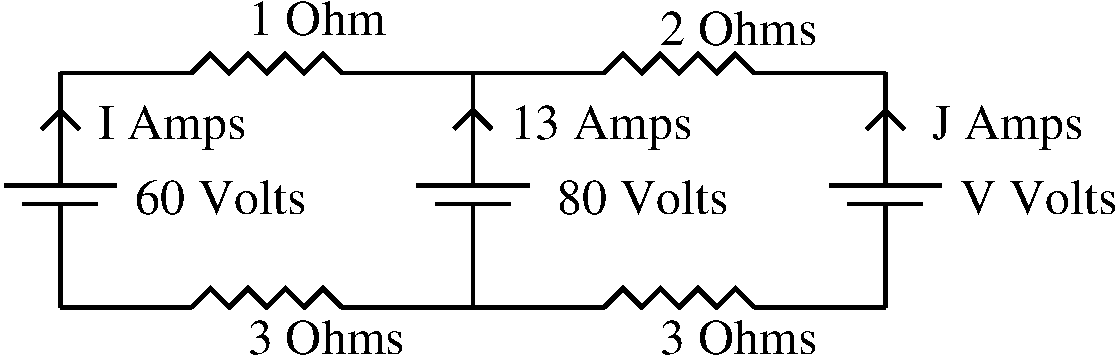
\includegraphics[scale=.6]{circuit.pdf}
$$
Find all possible equations for the unknowns $I$, $J$ and $V$ and then  solve for $I$, $J$ and $V$. Give your answers with correct units.



\item
Suppose $M$ is the matrix of a linear transformation 
$$
L: U\to V
$$
and the vector spaces $U$ and $V$ have dimensions
$$
\mbox{dim}\,  U= n\,,  \qquad \mbox{dim}\,  V= m\, , 
$$
and
$$
m\neq n\, .
$$
Also assume 
$$
\mbox{ker} L = \{0_U\}\, .
$$
\begin{enumerate}
\item How many rows does $M$ have? 
\item How many columns does $M$ have?
\item Are the columns of $M$ linearly independent?
\item What size matrix is $M^TM$?
\item What size matrix is $M M^T$?
\item Is $M^T M$ invertible?
\item is $M^T M$ symmetric? 
\item Is $M^TM$ diagonalizable?
\item  Does $M^TM$ have a zero eigenvalue?
\item Suppose $U=V$ and $\ker L\neq\{0_U\}$. Find an eigenvalue of $M$.
\item  Suppose $U=V$ and $\ker L\neq\{0_U\}$. Find $\det M$.
\end{enumerate}

\item Consider the system of equations
$$
\begin{array}{ccccccccc}
x&+&y&+&z&+&w&=&1\\
x&+&2y&+&2z&+&2w&=&1\\
x&+&2y&+&3z&+&3w&=&1\\
\end{array}
$$
Express this system as a matrix equation $MX=V$ and then find the solution set by computing an $LU$ 
decomposition for the matrix $M$ (be sure to use back and forward substitution).

\item
Compute the following determinants
$$
\det\begin{pmatrix}1&2\\3&4
\end{pmatrix},\:
\det\begin{pmatrix}1&2&3\\4&5&6\\7&8&9
\end{pmatrix},\:
\det\begin{pmatrix}1&2&3&4\\5&6&7&8\\9&10&11&12\\13&14&15&16
\end{pmatrix} ,\:$$ $$
\det\begin{pmatrix}1&2&3&4&5\\6&7&8&9&10\\11&12&13&14&15\\
16&17&18&19&20\\21&22&23&24&25
\end{pmatrix}.
$$
Now test your skills on
$$
\det\left(\begin{array}{ccccc}1&2&3&\cdots&n\\n+1&n+2&n+3&\cdots&2n\\2n+1&2n+2&2n+3&&3n \\
\vdots&&&\ddots&\vdots\\n^2-n+1&n^2-n+2&n^2-n+3&\cdots&n^2
\end{array}\right).
$$
{\it Make sure to jot down a few brief notes explaining any clever tricks you use.}

\item
For which values of $a$ does $$U={\rm span} \left\{
\begin{pmatrix}1\\0\\1\end{pmatrix},\begin{pmatrix}1\\2\\-3\end{pmatrix},\begin{pmatrix}a\\1\\0\end{pmatrix}\right\}={\mathbb R}^3\ ?$$
 For any special values of $a$ at which $U\neq{\mathbb R}^3$, express the subspace $U$ as the span of the least number of vectors possible. Give the dimension of $U$ for these cases and
 draw a picture showing $U$ inside ${\mathbb R}^3$.

\item
{\it Vandermonde determinant:}\index{Vandermonde determinant} Calculate the following determinants
$$
\det \begin{pmatrix}1 & x\\ 1 & y\end{pmatrix}\, ,\quad
\det \begin{pmatrix}1 & x & x^2\\ 1 & y&y^2\\ 1& z&z^2\end{pmatrix}\, ,\quad
\det \begin{pmatrix}1 & x & x^2 & x^3\\ 1 & y& y^2 & y^3\\ 1 & z & z^2 & z^3\\ 1 & w & w^2 & w^3\end{pmatrix}\, .
$$
Be sure to factorize you answers, if possible.

{\it Challenging:} Compute the determinant
$$
\det \begin{pmatrix}1 & x_1 & (x_1)^2 & \cdots &(x_1)^{n-1}\\ 
1 & x_2& (x_2)^2 & \cdots &  (x_2)^{n-1}\\ 
1 & x_3& (x_3)^2 & \cdots &  (x_3)^{n-1}\\ 
\vdots &\vdots &\vdots &\ddots & \vdots\ \ \  \\ 
1 & x_n& (x_n)^2 & \cdots &  (x_n)^{n-1}\end{pmatrix}\, .
$$

\item
\begin{enumerate}\item Do the vectors $\left\{\begin{pmatrix}1\\2\\3\end{pmatrix},\begin{pmatrix}3\\2\\1\end{pmatrix},\begin{pmatrix}1\\0\\0\end{pmatrix},\begin{pmatrix}0\\1\\0\end{pmatrix},\begin{pmatrix}0\\0\\1\end{pmatrix}\right\}$ form a basis for ${\mathbb R}^3$? {\it Be sure to justify your answer.}
\item
Find a basis for ${\mathbb R}^4$ that includes the vectors $\begin{pmatrix}1\\2\\3\\4\end{pmatrix}$
and $\begin{pmatrix}4\\3\\2\\1\end{pmatrix}$.
\item Explain in words how to generalize your computation in part (b) to obtain a basis for ${\mathbb R}^n$ that includes a given pair of (linearly independent) vectors $u$ and $v$. 
\end{enumerate}

\item 
Elite NASA engineers\index{Elite NASA engineers} determine that if a satellite is placed in orbit starting at a point ${\cal O}$, it will return
exactly to that same point after one orbit of the earth. Unfortunately, if there is a small mistake in the original location of the 
satellite, which the engineers label by a vector $X$ in ${\mathbb R}^3$ with origin\footnote{This is a spy satellite. The exact location of ${\cal O}$, the orientation of the coordinate axes in ${\mathbb R}^3$ and the unit system employed by the engineers are CIA secrets.} 
at~${\cal O}$, after one orbit the satellite will instead return to some other point $Y\in {\mathbb R}^3$. The engineer's computations
show that $Y$ is related to $X$ by a matrix
$$
Y = \begin{pmatrix} 0&\frac12 & 1 \\[2mm] \frac12 &\frac12 &\frac 12 \\[2mm] 1 & \frac 12 &0\end{pmatrix} X\, .
$$
\begin{enumerate}
\item Find all eigenvalues of the above matrix.
\item Determine  {\it all} possible eigenvectors associated with each eigenvalue.
\end{enumerate}
Let us assume that the rule found by the engineers applies to all subsequent orbits. 
Discuss case by case, what will happen to the satellite if the initial mistake in its location
is in a direction given by an eigenvector. 
\item
In this problem the scalars in the vector spaces are bits ($0,1$ with $1+1=0$). The space $B^k$ is the vector space of bit-valued, $k$-component column vectors.
\begin{enumerate}
\item
Find a basis for $B^3$. 
\item Your answer to part (a) should be a list of vectors $v_1$, $v_2,\ldots v_n$. What number did you find for $n$? 
\item How many elements are there in the {\it set} $B^3$. 
\item What is the dimension of the vector space $B^3$. 
\item Suppose $L:B^3\to B=\{0,1\}$ is a linear transformation. Explain why specifying $L(v_1)$, $L(v_2),\ldots,L(v_n)$ completely determines $L$. 
\item Use the notation of 
part (e) to list {all} linear transformations $$L:B^3\to B\, .$$
How many different linear transformations did you find? Compare your answer to part (c). 
\item Suppose $L_1:B^3\to B$ and $L_2: B^3\to B$ are linear transformations, and $\alpha$ and $\beta$ are bits.
Define a new map 
$(\alpha L_1+\beta L_2):B^3\to B$ by $$(\alpha L_1+\beta L_2)(v)=\alpha L_1(v)+\beta L_2(v).$$ Is this map a linear transformation? Explain.
\item Do you think the set of all linear transformations from $B^3$ to $B$ is a vector space using the addition rule above? If you answer yes, 
give a basis for this vector space and state its dimension.
\end{enumerate}

\item
A team of distinguished, post-doctoral engineers analyzes the design for a bridge across the
English channel. They notice that the force on the center of the bridge when it is displaced
by an amount $X=\begin{pmatrix}x\\y\\z\end{pmatrix}$ is given by 
$$
F=\ccolvec{-x-y\\-x-2y-z\\-y-z}\, .
$$
Moreover, having read Newton's Principi\ae\index{Newton's Principi\ae}, they know that force is proportional to acceleration so that\footnote{The bridge is intended for French and English military vehicles, so the exact units, coordinate system and constant of proportionality are state secrets.}
$$
F=\frac{d^2 X}{dt^2}\, .
$$
Since the engineers are worried the bridge might start swaying in the heavy channel winds, they search for 
an oscillatory  solution to this equation of the form\footnote{Here, $a,b,c$ and $\omega$ are constants which we aim to calculate.}
$$
X=\cos(\omega t) \ \begin{pmatrix} a \\ b \\ c\end{pmatrix}\, .
$$
\begin{enumerate}
\item By plugging their proposed solution in the above equations the engineers find an eigenvalue problem
$$
M \begin{pmatrix} a \\ b \\ c\end{pmatrix} = -\omega^2 \begin{pmatrix} a \\ b \\ c\end{pmatrix}\, .
$$
Here $M$ is a $3\times 3$ matrix. Which $3\times 3$ matrix  $M$ did the engineers find?
{\it Justify your answer.}
\item
Find the eigenvalues and eigenvectors of the matrix $M$.
\item The number $|\omega|$ is often called a {\it characteristic frequency}. What characteristic
frequencies do you find for the proposed bridge?
\item Find an orthogonal matrix $P$ such that $MP=PD$ where $D$ is a diagonal matrix.
{\it Be sure to also state your result for $D$.}
\item Is there a direction in which displacing the bridge yields no force? If so give a vector in that direction.
{\it Briefly} evaluate the quality of this bridge design.
\end{enumerate}


\item{\it Conic Sections}:\index{Conic sections} The equation for the most general conic section is given~by
$$
ax^2 + 2bxy+dy^2 + 2cx+2ey + f=0\, . 
$$
Our aim is to analyze the solutions to this equation using matrices.
\begin{enumerate}
\item \label{parta}Rewrite the above quadratic equation as one of the form $$X^T M X +  X^T C + C^T X+ f=0$$ relating an unknown column vector $X=\begin{pmatrix}x
 \\ y\end{pmatrix}$, its transpose $X^T$, a $2\times 2$ matrix $M$, a constant column vector $C$ and the  constant~$f$.
\item Does your matrix $M$ obey any special properties? Find its eigenvalues. You may call your answers $\lambda$ and $\mu$ for the rest of the problem to save writing.
\begin{quote}{\it For the rest of this problem we will focus on central conics for which the matrix $M$ is invertible.}\end{quote}
\item Your equation in part (a) above should be be quadratic in $X$. Recall that if $m\neq 0$, 
the quadratic equation $mx^2 + 2cx+f=0$ can be rewritten by {\it completing the square}
$$
m\Big(x+\frac cm\Big)^2 = \frac{c^2}{m}-f\, .
$$
Being very careful that you are now dealing with matrices, use the same trick to rewrite your answer to part (a) in the form
$$
Y^T M Y = g.
$$
Make sure you give formulas for the new unknown column vector~$Y$ and constant $g$ in terms of $X$, $M$, $C$ and $f$. You need not multiply out any of the matrix expressions you find.
\begin{quote}{\it 
If all has gone well, you have found a way to shift coordinates for the original conic equation
to a new coordinate system with its origin at the center of symmetry. Our next aim is to rotate the coordinate
axes to produce a readily recognizable equation.}
\end{quote}
\item Why is the angle between vectors $V$ and $W$ is not changed when you replace
them by $PV$ and $PW$ for $P$ any orthogonal matrix?
\item Explain how to choose an orthogonal  matrix $P$ such that $MP=PD$ where $D$ is a diagonal matrix.
\item For the choice of $P$ above, define our final unknown vector $Z$ by $Y=PZ$. Find an expression for $Y^T MY$ in terms of $Z$ and the eigenvalues of $M$.
\item Call $Z=\begin{pmatrix}z\\w\end{pmatrix}$. What equation do $z$ and $w$ obey?
(Hint, write your answer using $\lambda$, $\mu$ and $g$.)
\item Central conics are circles, ellipses, hyperbolae or a pair of straight lines. Give examples of values of 
$(\lambda,\mu,g)$ which produce each of these cases.

\end{enumerate}

\item Let \(L \colon V \to W\) be a linear transformation between finite-dimensional vector spaces \(V\) and \(W\), and let \(M\) be a matrix for \(L\) (with respect to some basis for \(V\) and some basis for \(W\)). We know that \(L\) has an inverse if and only if it is bijective, and we know a lot of ways to tell whether \(M\) has an inverse. In fact, \(L\) has an inverse if and only if \(M\) has an inverse:
\begin{enumerate}
\item Suppose that \(L\) is bijective (i.e., one-to-one and onto).
\begin{enumerate}
\item Show that \(\dim V=\rank L=\dim W\).
\item Show that \(0\) is not an eigenvalue of \(M\).
\item Show that \(M\) is an invertible matrix. 
\end{enumerate}
\item Now, suppose that \(M\) is an invertible matrix.
\begin{enumerate}
\item Show that \(0\) is not an eigenvalue of \(M\).
\item Show that \(L\) is injective.
\item Show that \(L\) is surjective.
\end{enumerate}
\end{enumerate}

\item Captain Conundrum gives Queen Quandary\index{Queen Quandary} a pair of newborn doves, male and female for her birthday. After one year, this pair of doves breed and produce a pair of dove eggs. One year later these eggs hatch yielding a new pair of doves while the original pair of doves breed again and an additional pair of eggs are laid.  Captain Conundrum is
very happy because now he will never need to buy the Queen a present ever again! 

Let us say that in year zero, the Queen has no doves. In year one she has one pair of doves, in year two she has two pairs of doves {\it etc...}
Call $F_n$ the number of pairs of doves in  years~$n$. For example, $F_0=0$, $F_1=1$ and $F_2=1$. Assume no doves die and that the same breeding pattern continues well into the future. Then $F_3=2$ because the eggs laid by the first pair of doves in year two hatch. Notice also that in year three,  two pairs of eggs are laid (by the first and second pair of doves). Thus $F_4=3$.
\begin{enumerate}
\item Compute $F_5$ and $F_6$.
\item Explain why (for any $n\geq 2$) the following {\it recursion relation}\index{Recursion relation}  holds
$$
F_n=F_{n-1}+F_{n-2}\, .
$$
\item Let us introduce a column vector
$X_n=\begin{pmatrix}\mc{F_n}\\F_{n-1}\end{pmatrix}
$. Compute $X_1$ and~$X_2$. Verify that these vectors obey the relationship
$$
X_2=M X_1 \mbox{ where } M=\begin{pmatrix}1 & 1\\1 & 0\end{pmatrix}\, . $$
\item Show that $X_{n+1}=M X_{n}$.
\item Diagonalize $M$. ({\it I.e.}, write $M$ as a product $M=PDP^{-1}$ where $D$ is diagonal.)
\item Find a simple expression for $M^n$ in terms of $P$, $D$ and $P^{-1}$.
\item Show that $X_{n+1}=M^n X_1$.
\item The number
$$\varphi=\frac{1+\sqrt{5}}2 $$
is called the {\it golden ratio}\index{Golden ratio}. Write the eigenvalues of $M$ in terms of~$\varphi$.
\item Put your results from parts (c), (f) and (g) together (along with a short matrix computation) to find
the formula for the number of doves  $F_n$ in year~$n$ expressed in terms of $\varphi$, $1-\varphi$ and $n$.
\end{enumerate}

\item
Use Gram--Schmidt to find an orthonormal basis for
$$
\mbox{span} 
\left\{
\begin{pmatrix}
1\\1\\1\\1
\end{pmatrix}\, ,\,
\begin{pmatrix}
1\\0\\1\\1
\end{pmatrix}\, ,\,
\begin{pmatrix}
0\\0\\1\\2
\end{pmatrix}
\right\}\, .
$$

\item Let $M$ be the matrix of a linear transformation $L:V\to W$ in given bases for $V$ and $W$.
Fill in the blanks below with one of the following six vector spaces: $V$, $W$, ${\rm ker} L$, 
$\big({\rm ker} L\big)^\perp$, ${\rm im} L$, $\big({\rm im} L\big)^\perp$.
\begin{enumerate}
\item The columns of $M$ span \underline{\phantom{answer}} in the basis given for \underline{\phantom{answer}}.
\item The rows of $M$ span \underline{\phantom{answer}} in the basis given for \underline{\phantom{answer}}.
\end{enumerate} 
Suppose $$M=\begin{pmatrix}1&2&1&3\\2&1&\!-1&2\\1&0&0&\!-1\\4&1&\!-1&0\end{pmatrix}$$
is the matrix of $L$ in the bases $\{v_1,v_2,v_3,v_4\}$ for $V$ and $\{w_1,w_2,w_3,w_4\}$ for~$W$.
Find bases for ${\rm ker} L$ and ${\rm im} L$. Use the dimension formula to check your result.

\item
Captain Conundrum collects the following data set
$$
\begin{array}{c|c}
y&x\\
\hline
5&-2\\
2&-1\\
0&1\\
3&2
\end{array}
$$
which he believes to be well-approximated by a parabola
$$
y=ax^2+bx+c\, .
$$

\begin{enumerate}
\item Write down a system of four linear equations for the unknown coefficients $a$, $b$ and $c$.
\item Write the augmented matrix for this system of equations.
\item Find the reduced row echelon form for this augmented matrix.
\item Are there any solutions to this system?
\item Find the least squares solution to the system.
\item What value does Captain Conundrum predict for $y$ when $x=2$? 
\end{enumerate}


\item Suppose you have collected the following data for an experiment
$$
\begin{array}{l|l}
x&y\\\hline
x_1&y_1\\
x_2&y_2\\
x_3&y_3
\end{array}
$$
and believe that the result is well modeled by a straight line
$$
y=mx+b\, .
$$
\begin{enumerate}
\item Write down a linear system of equations you could use to find the slope $m$ and constant term~$b$. 
\item Arrange the unknowns $(m,b)$ in a column vector $X$ and write your answer to (a) as a matrix equation $$M X= V\, .$$
Be sure to give explicit expressions for the matrix $M$ and column vector $V$.
\item For a generic data set, would you expect your system of equations to have a solution? {\it Briefly} explain your answer.
\item Calculate $M^T M$ and $(M^T M)^{-1}$ (for the latter computation, state the condition required for the inverse to exist).
\item Compute the least squares solution for $m$ and $b$.
\item The least squares method determines a vector $X$ that minimizes the length of the vector $V-MX$. Draw a rough sketch of
the three data points in the $(x,y)$-plane as well as their least squares fit. 
Indicate how the components of $V-MX$ could be obtained from your picture.

\end{enumerate}

\end{enumerate}

\subsection*{Solutions}

\begin{enumerate}
\item You can find the definitions for all these terms by consulting the index of this book.

\item Both junctions give the same equation for the currents
$$
I+J+13=0\, .
$$
There are three voltage loops (one on the left, one on the right and one going around the outside of the circuit). Respectively, they give the equations
\begin{eqnarray}
&60-I-80-3I=0&\nn\\[2mm]
&80+2J-V+3J=0&\nn\\[2mm]
&60-I+2J-V+3J-3I=0&\, .
\end{eqnarray}
The above equations are easily solved (either using an augmented matrix and row reducing, or by substitution). The result is $I=-5$ Amps, $J=-8$ Amps, $V=40$ Volts.



\item 
\begin{enumerate}
\item $m$.
\item $n$.
\item Yes.
\item $n\times n$.
\item $m\times m$.
\item Yes. This relies on ${\rm ker} M=0$ because if $M^T M$ had a non-trivial kernel, then there would be a non-zero solution $X$ to $M^T M X=0$. But then by multiplying on the left by $X^T$ we see that $||MX||=0$. This in turn implies $MX=0$ which contradicts the triviality of the kernel of $M$. 
\item Yes because $\big(M^T M\big)^T=M^T (M^T)^T=M^T M$.
\item Yes, all symmetric matrices have a basis of eigenvectors.
\item No, because otherwise it would not be invertible.
\item Since the kernel of $L$ is non-trivial, $M$ must have $0$ as an eigenvalue.
\item Since $M$ has a zero eigenvalue in this case, its determinant must vanish. {I.e.}, $\det M=0$.
\end{enumerate}

\item To begin with the system becomes
$$
\begin{pmatrix}1&1&1&1\\[1mm]1&2&2&2\\[1mm]1&2&3&3
\end{pmatrix}
\begin{pmatrix}x\\[1mm]y\\[1mm]z\\[1mm]w\end{pmatrix}=
\begin{pmatrix}1\\[1mm]1\\[1mm]1\end{pmatrix}
$$
Then
$$
M=
\begin{pmatrix}
1&1&1&1\\[1mm]1&2&2&2\\[1mm]1&2&3&3
\end{pmatrix}
=
\begin{pmatrix}
1&0&0\\[1mm]1&1&0\\[1mm]1&0&1
\end{pmatrix}
\begin{pmatrix}
1&1&1&1\\[1mm]0&1&1&1\\[1mm]0&1&2&2
\end{pmatrix}$$ $$
=
\begin{pmatrix}
1&0&0\\[1mm]1&1&0\\[1mm]1&1&1
\end{pmatrix}
\begin{pmatrix}
1&1&1&1\\[1mm]0&1&1&1\\[1mm]0&0&1&1
\end{pmatrix}=LU
$$
So now $MX=V$ becomes $LW=V$ where $W=UX=\begin{pmatrix}a\\b\\c\end{pmatrix}$ (say). Thus we solve $LW=V$ by forward substitution
$$
a=1,\ a+b=1,  \ a+b+c=1 \Rightarrow a=1,b=0,c=0\, .
$$
Now solve $UX=W$ by back substitution
$$
x+y+z+w=1, \ y+z+w=0, \ z + w =0$$ $$ \ \Rightarrow
w=\mu \mbox{ (arbitrary)}, z=-\mu, y=0, x=1\, .
$$
The solution set is $\left\{\begin{pmatrix}x\\y\\z\\y\end{pmatrix}=\begin{pmatrix}1\\0\\-\mu\\\mu\end{pmatrix}: \mu\in {\mathbb R}\right\}$


\item First 
$$\det\begin{pmatrix}1&2\\3&4\end{pmatrix}=-2\, .$$
All the other determinants vanish because the first three rows of each matrix are not independent. 
Indeed, $2R_2-R_1=R_3$ in each case, so we can make row operations to get a row of zeros and thus a zero determinant. 

\item If $U$ spans ${\mathbb R}^3$, then we must be able to express any vector $X=\begin{pmatrix}x\\y\\z\end{pmatrix}$ $\in {\mathbb R}^3$
as
$$
X=c^1\begin{pmatrix}1\\0\\1\end{pmatrix}+c^2\begin{pmatrix}1\\2\\-3\end{pmatrix}+c^3\begin{pmatrix}a\\1\\0\end{pmatrix}
=\begin{pmatrix}1&1&a\\0&2&1\\1&-3&0\end{pmatrix}\begin{pmatrix}c^1\\c^2\\c^3\end{pmatrix}\, ,
$$
for some coefficients $c^1$, $c^2$ and $c^3$. This is a linear system. We could solve for $c^1$, $c^2$ and $c^3$ using an
augmented matrix and row operations. However, since we know that ${\rm dim}\, {\mathbb R}^3=3$, if $U$ spans ${\mathbb R}^3$,
it will also be a basis. Then the solution for  $c^1$, $c^2$ and $c^3$ would be unique. Hence, the $3\times 3$ matrix above must 
be invertible, so we examine its determinant
$$
{\rm det} \begin{pmatrix}1&1&a\\0&2&1\\1&-3&0\end{pmatrix}
=1.(2.0-1.(-3))+1.(1.1-a.2)=4-2a\, .
$$
Thus $U$ spans ${\mathbb R}^3$ whenever $a\neq 2$. When $a=2$ we can write the third vector in $U$ in terms of the preceding ones as
$$
\begin{pmatrix}2\\1\\0\end{pmatrix}=\frac32\begin{pmatrix}1\\0\\1\end{pmatrix}+\frac12\begin{pmatrix}1\\2\\-3\end{pmatrix}.
$$
({\it You can obtain this result, or an equivalent one by studying the above linear system with $X=0$, i.e., the associated homogeneous system.}) The two vectors $\begin{pmatrix}1\\2\\-3\end{pmatrix}$ and $\begin{pmatrix}2\\1\\0\end{pmatrix}$ are clearly linearly independent,
so this is the least number of vectors spanning $U$ for this value of $a$. Also we see that dim$U=2$ in this case. Your picture should be
a plane in ${\mathbb R}^3$ though the origin  containing the vectors $\begin{pmatrix}1\\2\\-3\end{pmatrix}$ and $\begin{pmatrix}2\\1\\0\end{pmatrix}$.

\item 
$$
\det \begin{pmatrix}1 & x\\ 1 & y\end{pmatrix}=y-x\, ,\ \ 
$$

$$
\det \begin{pmatrix}1 & x & x^2\\ 1 & y&y^2\\ 1& z&z^2\end{pmatrix}=
\det \begin{pmatrix}1 & x & x^2\\ 0 & y-x&y^2-x^2\\ 0& z-x&z^2-x^2\end{pmatrix}$$ $$
=(y-x)(z^2-x^2)-(y^2-x^2)(z-x)=(y-x)(z-x)(z-y)\, .
$$

$$
\det \begin{pmatrix}1 & x & x^2 & x^3\\ 1 & y& y^2 & y^3\\ 1 & z & z^2 & z^3\\ 1 & w & w^2 & w^3\end{pmatrix}
=
\det \begin{pmatrix}1 & x & x^2 & x^3\\ 0 & y-x& y^2-x^2 & y^3-x^3\\ 0 & z-x & z^2 -x^2& z^3-x^3\\ 0 & w-x & w^2-x^2 & w^3-x^3\end{pmatrix}
$$
$$
=
\det \begin{pmatrix}1 & 0 & 0 & 0\\ 0 & y-x& y(y-x)& y^2(y-x)\\ 0 & z-x & z(z-x) & z^2(z-x)\\ 0 & w-x & w(w-x) & w^2(w-x)\end{pmatrix}
$$
$$=
(y-x)(z-x)(w-x)\det \begin{pmatrix}1 & 0 & 0 & 0\\ 0 & 1& y& y^2\\ 0 & 1 & z & z^2\\ 0 & 1 & w & w^2\end{pmatrix}
$$
$$
=(y-x)(z-x)(w-x)\det \begin{pmatrix}1 & y & y^2\\ 1 & z&z^2\\ 1& w&w^2\end{pmatrix}
$$
$$
=(y-x)(z-x)(w-x) (z-y)(w-y)(w-z)\, .
$$
From the $4\times 4$ case above, you can see all the tricks required for a general Vandermonde matrix.
First zero out the first column by subtracting the first row from all other rows (which leaves the determinant unchanged). Now zero out the top row by subtracting $x_1$ times the first column from the second column,
$x_1$ times the second column from the third column {\it et cetra}. Again these column operations do not
change the determinant. Now factor out $x_2-x_1$ from the second row, $x_3-x_1$ from the third row, {\it etc}. This does change the determinant so we write these factors outside the remaining determinant, which is just the same problem but for the $(n-1)\times(n-1)$ case. Iterating the same procedure gives the result
$$
\det \begin{pmatrix}1 & x_1 & (x_1)^2 & \cdots &(x_1)^{n-1}\\ 
1 & x_2& (x_2)^2 & \cdots &  (x_2)^{n-1}\\ 
1 & x_3& (x_3)^2 & \cdots &  (x_3)^{n-1}\\ 
\mc\vdots &\mc\vdots &\mc\vdots &\ddots & \mc\vdots\ \ \  \\ 
1 & x_n& (x_n)^2 & \cdots &  (x_n)^{n-1}\end{pmatrix}
=\prod_{i>j}(x_i-x_j)\, .
$$
(Here $\prod$ stands for a multiple product, just like $\Sigma$ stands for a multiple sum.)

\item \begin{enumerate}
\item No, a basis for  ${\mathbb R}^3$ must have exactly three vectors.
\item We first extend the original vectors by the standard basis for ${\mathbb R}^4$ and then try to eliminate two of them by considering
$$
\alpha \begin{pmatrix}1\\2\\3\\4\end{pmatrix}+\beta
\begin{pmatrix}4\\3\\2\\1\end{pmatrix} +\gamma 
\begin{pmatrix}1\\0\\0\\0\end{pmatrix}
+\delta\begin{pmatrix}0\\1\\0\\0\end{pmatrix}
+\varepsilon\begin{pmatrix}0\\0\\1\\0\end{pmatrix}
+\eta\begin{pmatrix}0\\0\\0\\1\end{pmatrix}=0\, .
$$ 
So we study
$$
\begin{pmatrix}
1&4&1&0&0&0\\
2&3&0&1&0&0\\
3&2&0&0&1&0\\
4&1&0&0&0&1
\end{pmatrix}
\sim
\begin{pmatrix}
1&4&1&0&0&0\\
0&-5&-2&1&0&0\\
0&-10&-3&0&1&0\\
0&-15&-4&0&0&1
\end{pmatrix}
$$
$$
\sim
\begin{pmatrix}
1&0&-\frac35&-4&0&0\\
0&1&\frac25&\frac15&0&0\\[1mm]
0&0&1&10&1&0\\
0&0&2&15&0&1
\end{pmatrix}
\sim
\begin{pmatrix}
1&0&0&2&\frac35&0\\
0&1&0&-\frac{19}5&-\frac25&0\\[1mm]
0&0&1&10&1&0\\
0&0&0&-\frac{5}2&-10&\frac12
\end{pmatrix}
$$
From here we can keep row reducing to achieve RREF, but we can already see that the non-pivot variables will be
$\varepsilon$ and $\eta$. Hence we can eject the last two vectors and obtain as our basis
$$
\left\{
\begin{pmatrix}1\\2\\3\\4\end{pmatrix},
\begin{pmatrix}4\\3\\2\\1\end{pmatrix},
\begin{pmatrix}1\\0\\0\\0\end{pmatrix},
\begin{pmatrix}0\\1\\0\\0\end{pmatrix}
\right\}\, .
$$
Of course, this answer is far from unique!
\item The method is the same as above. Add the standard basis to $\{u,v\}$ to obtain the linearly dependent set
$\{u,v,e_1,\ldots , e_n\}$. Then put these vectors as the columns of a matrix and row reduce. The  standard basis
vectors in columns corresponding to the non-pivot variables can be removed.
\end{enumerate}


\item 
\begin{enumerate}
\item
$$
{\rm det} \begin{pmatrix} \lambda&-\frac12 & -1 \\[2mm] -\frac12 &\lambda-\frac12 &-\frac12 \\[2mm] -1 & -\frac12 &\lambda\end{pmatrix}
=\lambda\Big((\lambda-\frac12\Big)\lambda-\frac14)+\frac12\Big(-\frac{\lambda}2-\frac12\Big)-\Big(-\frac14+\lambda\Big)
$$
$$
=\lambda^3-\frac{1}{2}\lambda^2-\frac32 \lambda=\lambda(\lambda+1)(\lambda-\frac32)\, .
$$
Hence the eigenvalues are $0,-1,\frac32$.
\item
When $\lambda=0$ we must solve the homogenous system
$$
\left(
\begin{array}{ccc|c}
0&\frac12&1&0\\[1mm]
\frac12&\frac12&\frac12&0\\[1mm]
1&\frac12&0&0
\end{array}\right)
\sim
\left(
\begin{array}{ccc|c}
1&\frac12&0&0\\[1mm]
0&\frac14&\frac12&0\\[1mm]
0&\frac12&1&0
\end{array}\right)
\sim
\left(
\begin{array}{ccc|c}
1&0&-1&0\\[1mm]
0&1&2&0\\[1mm]
0&0&0&0
\end{array}\right)\, .
$$
So we find the eigenvector $\begin{pmatrix}s\\-2s\\s\end{pmatrix}$ where $s\neq 0$ is arbitrary.

For $\lambda=-1$ 
$$
\left(
\begin{array}{ccc|c}
1&\frac12&1&0\\[1mm]
\frac12&\frac32&\frac12&0\\[1mm]
1&\frac12&1&0
\end{array}\right)
\sim
\left(
\begin{array}{ccc|c}
1&0&1&0\\[1mm]
0&1&0&0\\[1mm]
0&0&0&0
\end{array}\right)
\, .
$$
So we find the eigenvector $\begin{pmatrix}-s\\0\\s\end{pmatrix}$ where $s\neq 0$ is arbitrary.

Finally, for $\lambda=\frac32$
$$
\left(
\begin{array}{ccc|c}
-\frac32&\frac12&1&0\\[1mm]
\frac12&-1&\frac12&0\\[1mm]
1&\frac12&-\frac32&0
\end{array}\right)
\sim
\left(
\begin{array}{ccc|c}
1&\frac12&-\frac32&0\\[1mm]
0&-\frac54&\frac54&0\\[1mm]
0&\frac54&-\frac54&0
\end{array}\right)
\sim
\left(
\begin{array}{ccc|c}
1&0&-1&0\\[1mm]
0&1&-1&0\\[1mm]
0&0&0&0
\end{array}\right)\, .
$$
So we find the eigenvector $\begin{pmatrix}s\\s\\s\end{pmatrix}$ where $s\neq 0$ is arbitrary.
\end{enumerate}
If the mistake $X$ is in the direction of the eigenvector $\begin{pmatrix}1\\-2\\1\end{pmatrix}$,
then $Y=0$. {\it I.e.}, the satellite returns to the origin ${\cal O}$. For all subsequent orbits it will again return to 
the origin. NASA would be very pleased in this case.

If the mistake $X$ is in the direction $\begin{pmatrix}-1\\0\\1\end{pmatrix}$, then $Y=-X$. Hence the satellite will move to the point opposite to $X$. After next orbit will move back to $X$. It will continue this wobbling
motion indefinitely. Since this is a stable situation, again, the elite engineers will pat themselves on the back.

Finally, if the mistake  $X$ is in the direction $\begin{pmatrix}1\\1\\1\end{pmatrix}$ , the satellite will move
to a point $Y=\frac32 X$ which is further away from the origin. The same will happen for all subsequent
orbits, with the satellite moving a factor $3/2$ further away from ${\cal O}$ each orbit (in reality, after
several orbits, the approximations used by the engineers in their calculations probably fail and a new computation  will be needed). In this case, the satellite will be lost in outer space and the engineers will likely lose their jobs!

\item 
\begin{enumerate}
\item A basis for $B^3$ is $\left\{
\begin{pmatrix}1\\0\\0\end{pmatrix},
\begin{pmatrix}0\\1\\0\end{pmatrix},
\begin{pmatrix}0\\0\\1\end{pmatrix}
\right\}$
\item 3.
\item $2^3=8$.
\item dim$B^3=3$.
\item Because the vectors $\{v_1,v_2,v_3\}$ are a basis any element $v\in B^3$ can be
written uniquely as $v=b^1 v_1 +b^2 v_2+b^3 v_3$ for some triplet of bits~$\begin{pmatrix}b^1\\b^2\\b^3\end{pmatrix}$. Hence, to compute $L(v)$ we use linearity of $L$
$$
L(v) = L(b^1 v_1 +b^2 v_2+b^3 v_3) = b^1 L(v_1)  + b^2 L(v_2) + b^3 L(v_3) $$ $$= \begin{pmatrix}L(v_1) & L(v_2) & L(v_3)\end{pmatrix}
\begin{pmatrix}b^1\\b^2\\b^3\end{pmatrix}\, .
$$
\item From the notation of the previous part, we see that we can list  linear transformations $L:B^3\to B$
by writing out all possible bit-valued row vectors
\begin{eqnarray*}
&\begin{pmatrix}0 & 0 & 0\end{pmatrix} ,\\
&\begin{pmatrix}1 & 0 & 0\end{pmatrix} ,\\
&\begin{pmatrix}0 & 1 & 0\end{pmatrix} ,\\
&\begin{pmatrix}0 & 0 & 1\end{pmatrix} ,\\
&\begin{pmatrix}1 & 1 & 0\end{pmatrix} ,\\
&\begin{pmatrix}1 & 0 & 1\end{pmatrix} ,\\
&\begin{pmatrix}0 & 1 & 1\end{pmatrix} ,\\
&\begin{pmatrix}1 & 1  & 1\end{pmatrix} .
\end{eqnarray*}
There are $2^3=8$ different linear transformations $L:B^3\to B$, exactly the same as the number of elements in $B^3$.
\item Yes, essentially just because $L_1$ and $L_2$ are linear transformations. In detail for any bits
$(a,b)$ and vectors $(u,v)$ in $B^3$ it is easy to check the linearity property for $(\alpha L_1+\beta L_2)$
$$(\alpha L_1+\beta L_2)(a u + b v)=\alpha L_1(a u + b v)+\beta L_2(au + bv) 
$$
$$
=\alpha a L_1(u) + \alpha b L_1(v)+ \beta a L_1(u) + \beta b L_1(v) 
$$ $$= a (\alpha L_1(u) + \beta L_2(v))
+ b (\alpha L_1(u) + \beta L_2(v))
$$
$$
=a (\alpha L_1 + \beta L_2)(u) + b  (\alpha L_1 + \beta L_2)(v)\, .
$$
Here the first line used the definition of $(\alpha L_1 + \beta L_2)$, the second line depended on
the linearity of $L_1$ and $L_2$, the third line was just algebra and the fourth used the definition of $(\alpha L_1+ \beta L_2)$ again.
\item Yes. The easiest way to see this is the identification above of these maps with bit-valued column vectors. In that notation, a basis is 
$$\Big\{\begin{pmatrix}1&0&0\end{pmatrix},\begin{pmatrix}0&1&0\end{pmatrix},\begin{pmatrix}0&0&1\end{pmatrix}\Big\}\, .$$
Since this (spanning) set has three (linearly independent) elements, the vector space of linear maps $B^3\to B$ has dimension~3. This is an example of a general notion called the {\it dual vector space}\index{Dual vector space}.\end{enumerate}

\item 
\begin{enumerate}
\item $\frac{d^2 X}{dt^2}=\frac{d^2\cos(\omega t )}{dt^2}\colvec{a\\b\\c}=-\omega^2\cos(\omega t) \colvec{a\\b\\c}\, .$ 

Hence
\begin{eqnarray*}
F=\cos(\omega t) \ccolvec{-a-b\\-a-2b-c\\-b-c}&=&\cos(\omega t) \begin{pmatrix}-1&-1&0\\-1&-2&-1\\0&-1&-1\end{pmatrix}\colvec{a\\b\\c}
\\[1mm]&=&-\omega^2\cos(\omega t) \colvec{a\\b\\c}
\, ,\end{eqnarray*}
so 
$$
M=\begin{pmatrix}-1&-1&0\\-1&-2&-1\\0&-1&-1\end{pmatrix}\, .
$$
\item
\begin{eqnarray*}
\det \begin{pmatrix}\lambda+1&\mc1&\mc0\\\mc1&\lambda+2&\mc1\\\mc0&\mc1&\lambda+1\end{pmatrix}
&=&(\lambda+1)\big((\lambda+2)(\lambda+1)-1\big)-(\lambda+1)\\
&=&(\lambda+1)\big((\lambda+2)(\lambda+1)-2\big)\\
&=&(\lambda+1)\big(\lambda^2+3\lambda)=\lambda(\lambda+1)(\lambda+3)\end{eqnarray*}
so the eigenvalues are $\lambda=0,-1 ,-3 $.

For the eigenvectors, when $\lambda=0$ we study:
$$
M-0.I=\begin{pmatrix}-1&-1&0\\-1&-2&-1\\0&-1&-1\end{pmatrix}\sim\begin{pmatrix}1&1&0\\0&-1&-1\\0&-1&-1\end{pmatrix}
\sim\begin{pmatrix}1&0&\!-1\\0&1&1\\0&0&0\end{pmatrix}\, ,
$$
so $\colvec{1\\-1\\1}$ is an eigenvector.

For $\lambda=-1$
$$
M-(-1).I=\begin{pmatrix}0&-1&0\\-1&-1&-1\\0&-1&0\end{pmatrix}\sim\begin{pmatrix}1&0&1\\0&1&0\\0&0&0\end{pmatrix}
\, ,
$$
so $\colvec{-1\\0\\1}$ is an eigenvector.

For $\lambda=-3$
$$
M-(-3).I=\begin{pmatrix}2&-1&0\\-1&1&-1\\0&-1&2\end{pmatrix}\sim\begin{pmatrix}1&-1&1\\0&1&-2\\0&-1&2\end{pmatrix}
\sim\begin{pmatrix}1&0&-1\\0&1&-2\\0&0&0\end{pmatrix}\, ,
$$
so $\colvec{1\\2\\1}$ is an eigenvector.

\item The characteristic frequencies are $0,1,\sqrt{3}$.
\item The orthogonal change of basis matrix 
$$
P=\begin{pmatrix}
\frac1{\sqrt{3}}&-\frac1{\sqrt{2}}&\frac{1}{\sqrt{6}}\\
-\frac1{\sqrt{3}}&\mc 0&\frac{2}{\sqrt{6}}\\
\frac1{\sqrt{3}}&\frac1{\sqrt{2}}&\frac{1}{\sqrt{6}}
\end{pmatrix}
$$
It obeys $MP=PD$ where
$$
D=\begin{pmatrix}0&0&0\\0&-1&0\\0&0&-3\end{pmatrix}\, .
$$
\item Yes, the direction given by the eigenvector $\colvec{1\\-1\\1}$ because its eigenvalue is zero. This is probably a bad design for a bridge because it can be displaced in this direction with no force!
\end{enumerate}

\item 
\begin{enumerate}
\item If we call $M=\begin{pmatrix}a&b\\b&d\end{pmatrix}$, then $X^TMX=ax^2 + 2bxy + dy^2$.
Similarly putting $C=\begin{pmatrix}c\\e\end{pmatrix}$ yields $X^T C + C^T X = 2 X \dotprod C = 2 cx + 2 e y$. Thus
$$
0=
ax^2 + 2bxy + dy^2+2cx+2ey+f$$
$$=\begin{pmatrix} x & y\end{pmatrix} \begin{pmatrix}a&b\\b&d\end{pmatrix}
\begin{pmatrix} x \\ y\end{pmatrix}+ 
\begin{pmatrix} x & y\end{pmatrix}\begin{pmatrix}c\\e\end{pmatrix}+
\begin{pmatrix} c & e\end{pmatrix}\begin{pmatrix}x\\y\end{pmatrix}+f\, .
$$
\item Yes, the matrix $M$ is symmetric, so it will have a basis of eigenvectors and is similar to
a diagonal matrix of real eigenvalues.

To find the eigenvalues notice that $\det\begin{pmatrix}a-\lambda&b\\b&d-\lambda\end{pmatrix}
=(a-\lambda)(d-\lambda)-b^2=\big(\lambda-\frac{a+d}{2}\big)^2-b^2-\big(\frac{a-d}{2}\big)^2$.
So the eigenvalues are $$\lambda=\frac{a+d}{2}+\sqrt{b^2+\big(\frac{a-d}{2}\big)^2}
\mbox{ and } \mu=\frac{a+d}{2}-\sqrt{b^2+\big(\frac{a-d}{2}\big)^2}\, .$$
\item The trick is to write
$$X^T M X + C^T X + X^T C =(X^T+C^T M^{-1}) M (X+M^{-1} C) - C^T M^{-1} C\, ,$$
so that
$$(X^T+C^T M^{-1}) M (X+M^{-1} C) = C^T M C -f\, .$$
Hence $Y=X+M^{-1} C$ and $g=C^T M C -f$.
\item The cosine of the angle between vectors $V$ and $W$ is given by $$\frac{V\dotprod W}{\sqrt{V\dotprod V\, W\dotprod W}}=\frac{V^T W}{\sqrt{V^T V\, W^T W}}\, .$$ 
So replacing $V\to PV$ and $W\to PW$ will always give a factor $P^T P$ inside all the products, but $P^TP=I$ for orthogonal matrices. Hence none of the dot products in the above formula changes, so 
neither does the angle between $V$ and $W$.
\item If we take the eigenvectors of $M$, normalize them ({\it i.e.} divide them by their lengths),
and put them in a matrix $P$ (as columns) then $P$ will be an orthogonal matrix. (If it happens
that $\lambda=\mu$, then we also need to make sure the eigenvectors spanning the two dimensional
eigenspace corresponding to $\lambda$ are orthogonal.) Then, since $M$ times the eigenvectors
yields just the eigenvectors back again multiplied by their eigenvalues, it follows that $MP=PD$
where $D$ is the diagonal matrix made from eigenvalues.
\item If $Y=PZ$, then $Y^T M Y= Z^T P^T M P Z = Z^T P^T P D Z = Z^T D Z$ where $D=\begin{pmatrix}\lambda & 0 \\ 0&\mu \end{pmatrix}$.
\item Using part (f) and (c) we have 
$$\lambda z^2 + \mu w^2 = g\, .$$
\item When $\lambda=\mu$ and $g/\lambda=R^2$, we get the equation for a circle radius $R$ in the $(z,w)$-plane. When $\lambda$, $\mu$ and $g$ are postive, we have the equation for an ellipse. Vanishing $g$ along with $\lambda$ and $\mu$ of opposite signs gives a pair of straight lines.
When $g$ is non-vanishing, but $\lambda$ and $\mu$ have opposite signs, the result is a pair of hyperbol\ae. These shapes all come from cutting a cone with a plane, and are therefore called
conic sections.
\end{enumerate}

\item  We  show  that  \(L\)  is  bijective  if  and  only  if  \(M\)  is  invertible.
 		\begin{enumerate}
 		\item  We  suppose  that  \(L\)  is  bijective.
 		\begin{enumerate}
 		\item  Since  \(L\)  is  injective,  its  kernel  consists  of  the  zero  vector  alone.  Hence
 		\[
 		\null  L=\dim  \ker  L=0.
 		\]
 		So  by  the  Dimension  Formula,
 		\[
 		\dim  V=\null  L+\rank  L=\rank  L.
 		\]
 		Since  \(L\)  is  surjective,  \(L(V)=W.\)  Thus
 		\[
 		\rank  L=\dim  L(V)=\dim  W.
 		\]
 		Thereby  \[\dim  V=\rank  L=\dim  W.\]
 		\item  Since  \(\dim  V=\dim  W\),  the  matrix  \(M\)  is  square  so  we  can  talk  about  its  eigenvalues.  Since  \(L\)  is  injective,  its  kernel  is  the  zero  vector  alone.  That  is,  the  only  solution  to  \(LX=0\)  is  \(X=0_V\).  But  \(LX\)  is  the  same  as  \(MX\),  so  the  only  solution  to  \(MX=0\)  is  \(X=0_V\).  So  \(M\)  does  not  have  zero  as  an  eigenvalue.
 		\item  Since  \(MX=0\)  has  no  non-zero  solutions,  the  matrix  \(M\)  is  invertible.
	\end{enumerate}
 		\item  Now  we  suppose  that  \(M\)  is  an  invertible  matrix.
 		\begin{enumerate}
 		\item  Since  \(M\)  is  invertible,  the  system  \(MX=0\)  has  no  non-zero  solutions.  But  \(LX\)  is  the  same  as  \(MX\),  so  the  only  solution  to  \(LX=0\)  is  \(X=0_V\).  So  \(L\)  does  not  have  zero  as  an  eigenvalue.
 		\item  Since  \(LX=0\)  has  no  non-zero  solutions,  the  kernel  of  \(L\)  is  the  zero  vector  alone.  So  \(L\)  is  injective.
 		\item  Since  \(M\)  is  invertible,  we  must  have  that  \(\dim  V=\dim  W\).  By  the  Dimension  Formula,  we  have
 		\[
 		\dim  V=\null  L+\rank  L
 		\]
 		and  since  \(\ker  L=\{0_V\}\)  we  have  \(\null  L=\dim  \ker  L=0\),  so
 		\[
 		\dim  W=\dim  V=\rank  L=\dim  L(V).
 		\]
 		Since  \(L(V)\)  is  a  subspace  of  \(W\)  with  the  same  dimension  as  \(W\),  it  must  be  equal  to  \(W\).  To  see  why,  pick  a  basis  \(B\)  of  \(L(V)\).  Each  element  of  \(B\)  is  a  vector  in  \(W\),  so  the  elements  of  \(B\)  form  a  linearly  independent  set  in  \(W\).  Therefore  \(B\)  is  a  basis  of  \(W\),  since  the  size  of  \(B\)  is  equal  to  \(\dim  W\).  So  \(L(V)=\spa  B=W.\)  So  \(L\)  is  surjective.
 		\end{enumerate}
 		\end{enumerate}

\item 
\begin{enumerate}
\item $F_4=F_2+F_3=2+3=5$.
\item The number of pairs of doves in any given year equals the number of the previous years plus those that hatch and there are as many of them as pairs of doves in the year before the previous year.
\item $X_1=\begin{pmatrix}F_1\\F_0\end{pmatrix}=\begin{pmatrix}1\\0\end{pmatrix}$
and $X_2=\begin{pmatrix}F_2\\F_1\end{pmatrix}=\begin{pmatrix}1\\1\end{pmatrix}$.
$$
MX_1=\begin{pmatrix}1 & 1\\ 1& 0\end{pmatrix}\begin{pmatrix}1\\ 0\end{pmatrix}
=\begin{pmatrix}1\\1\end{pmatrix}=X_2\, .
$$
\item We just need to use the recursion relationship of part (b) in the top slot of $X_{n+1}$:
$$
X_{n+1}=\ccolvec{F_{n+1}\\F_n}
=\ccolvec{F_{n}+F_{n-1}\\F_n}=
\begin{pmatrix}1 & 1\\ 1& 0\end{pmatrix}\ccolvec{F_{n}\\F_{n-1}}=M X_n\, .
$$
\item Notice $M$ is symmetric so this is guaranteed to work. $$\det \begin{pmatrix}1-\lambda&\mc1\\\mc1&-\lambda\end{pmatrix}=\lambda(\lambda-1)-1=\big(\lambda-\frac12\big)^2-\frac54\, ,$$
so the eigenvalues are $\frac{1\pm\sqrt{5}}{2}$. Hence the eigenvectors are $\ccolvec{\frac{1\pm\sqrt{5}}{2}\\1}$, respectively (notice that $\frac{1+\sqrt{5}}{2}+1=\frac{1+\sqrt{5}}{2}.\frac{1+\sqrt{5}}{2}$ and $\frac{1-\sqrt{5}}{2}+1=\frac{1-\sqrt{5}}{2}.\frac{1-\sqrt{5}}{2}$).
Thus $M=PDP^{-1}$ with $$D=\begin{pmatrix}\frac{1+\sqrt{5}}{2}&\mc0\\[1mm]\mc0&\frac{1-\sqrt{5}}{2}\end{pmatrix} \mbox{ and } P =\begin{pmatrix}\frac{1+\sqrt{5}}{2}&\frac{1-\sqrt{5}}{2}\\[1mm]\mc1&\mc1\end{pmatrix}\, .$$
\item $M^n=(P D P^{-1})^n = P D P^{-1} P D P^{-1} \ldots P D P^{-1} = P D^n P^{-1}$.
\item Just use the matrix recursion relation of part (d) repeatedly: $$X_{n+1}= M X_{n} = M^2 X_{n-1}=\cdots = M^{n} X_1\, .$$
\item The eigenvalues are $\varphi = \frac{1+\sqrt{5}}{2}$ and $1-\varphi = \frac{1-\sqrt{5}}{2}$.
\item $$X_{n+1}=\ccolvec{F_{n+1}\\F_n}=
M^n X_n = P D^n P^{-1} X_{1}$$ $$=P 
\begin{pmatrix}\varphi&\mc0\\\mc0&1-\varphi\end{pmatrix}^{\!n} 
\begin{pmatrix}\frac{1}{\sqrt{5}}&\star \\-\frac{1}{\sqrt{5}}& \star\end{pmatrix}
\begin{pmatrix}1\\ 0\end{pmatrix}
=P 
\begin{pmatrix}\varphi^n&\mc0\\\mc0&(1-\varphi)^n\end{pmatrix}
\begin{pmatrix}\frac{1}{\sqrt{5}}\\-\frac{1}{\sqrt{5}}\end{pmatrix}
$$
$$
=\begin{pmatrix}\frac{1+\sqrt{5}}{2}&\frac{1-\sqrt{5}}{2}\\[1mm]\mc1&\mc1\end{pmatrix}
\begin{pmatrix}\mc{\frac{\varphi^n}{\sqrt{5}}}\\[1mm]-\frac{(1-\varphi)^n}{\sqrt{5}}\end{pmatrix}
=\begin{pmatrix}\mc\star \\[1mm]\frac{\varphi^n-(1-\varphi)^n}{\sqrt{5}}\end{pmatrix}.
$$
Hence
$$F_n=\frac{\varphi^n-(1-\varphi)^n}{\sqrt{5}}\, .$$
These are the famous Fibonacci numbers\index{Fibonacci numbers}.
\end{enumerate}


\item Call the three vectors $u,v$ and $w$, respectively. Then
$$
v^\perp=v-\frac{u\dotprod v}{u\dotprod u} u =v-\frac34 u = \begin{pmatrix}\frac14 \\[1mm] -\frac34 \\[1mm] \frac14\\[1mm] \frac14\end{pmatrix}\, ,
$$
and
$$
w^\perp = w - \frac{u\dotprod w}{u\dotprod u} u-\frac{v^\perp\dotprod w}{v^\perp\dotprod v^\perp} v^\perp
=w-\frac{3}{4} u -\frac{\frac34}{\frac34}v^\perp =\begin{pmatrix}-1\\0\\0\\1\end{pmatrix}
$$
Dividing by lengths, an orthonormal basis for ${\rm span}\{u,v,w\}$ is
$$
\left\{\begin{pmatrix}\frac12\\[2mm]\frac12\\[2mm]\frac12\\[2mm]\frac12\end{pmatrix},
\begin{pmatrix}\frac{\sqrt{3}}6\\[1mm]-\frac{\sqrt{3}}2\\[1mm]\frac{\sqrt{3}}6\\[1mm]\frac{\sqrt{3}}6\end{pmatrix},
\begin{pmatrix}-\frac{\sqrt{2}}2\\[1mm]\mc0\\[1mm]\mc0\\[1mm]\frac{\sqrt{2}}2\end{pmatrix}
\right\}\, .
$$
\item 

\begin{enumerate}
\item The columns of $M$ span ${\rm im} L$ in the basis given for $W$.
\item The rows of $M$ span $({\rm ker}L)^\perp$% in the basis given for $V$.
\item First we put $M$ in RREF:
\begin{eqnarray*}
M& = & \begin{pmatrix}1&2&1&3\\2&1&\!-1&2\\1&0&0&\!-1\\4&1&\!-1&0\end{pmatrix}
\ \sim\
\begin{pmatrix}1&2&1&3\\0&-3&-3&-4\\0&-2&-1&-4\\0&-7&-5&\!-12\end{pmatrix}\\[2mm]
&\sim& 
\begin{pmatrix}1&0&-1&\frac13\\[1mm]0&1&1&\frac43\\[1mm]0&0&1&-\frac43\\[1mm]0&0&2&-\frac83\end{pmatrix}
\ \sim\ \begin{pmatrix}1&0&0&-1\\[1mm]0&1&0&\frac83\\[1mm]0&0&1&-\frac43\\[1mm]0&0&0&0\end{pmatrix}\, .
\end{eqnarray*}
Hence $$\ker L=\spa\{v_1-\frac83v_2+\frac43 v_3+v_4\}$$ and $${\rm im} L=\spa\{v_1+2v_2+v_3+4v_4,2v_1+v_2+v_4,v_1-v_2-v_4\}\, .$$
Thus $\dim\ker L=1$ and $\dim{\rm im} L=3$ so $$\dim\ker L+\dim{\rm im} L=1+3=4=\dim V\, .$$
\end{enumerate}

\item 
\begin{enumerate}
\item
$$
\left\{
\begin{array}{l}
5=4a-2b+c\\
2=a-b+c\\
0=a+b+c\\
3=4a+2b+c\, .
\end{array}
\right.
$$
\item[(b,c,d)]
$$
\left(
\begin{array}{rrr|r}
4&-2&1&5\\
1&-1&1&2\\
1&1&1&0\\
4&2&1&3
\end{array}
\right)
\sim
\left(
\begin{array}{rrr|r}
1&1&1&0\\
0&-6&-3&5\\
0&-2&0&2\\
0&-2&-3&3
\end{array}
\right)
\sim
\left(
\begin{array}{rrr|r}
1&0&1&-1\\
0&1&0&1\\
0&0&-3&11\\
0&0&-3&3
\end{array}
\right)
$$
The system has no solutions because $c=-1$ and $c=-\frac{11}{3}$ is impossible.
\item[(e)]
Let $$M=\begin{pmatrix}
4&-2&1\\
1&-1&1\\
1&1&1\\
4&2&1
\end{pmatrix}\mbox{ and }
V=\colvec{5\\2\\0\\3}\, .$$
Then 
$$
M^T M=\begin{pmatrix}34&0&10\\0&10&0\\10&0&4\end{pmatrix}
\mbox{ and } 
M^TV=\colvec{34\\-6\\10}\, .
$$
So 
$$
\begin{amatrix}{3}
 34&0&10&34\\0&10&0&-6\\10&0&4&10
\end{amatrix}
~\sim
\begin{amatrix}{3}
1&0&\frac25&1\\0&10&0&-6\\0&0&-\frac{18}5&0
\end{amatrix}
~\sim
\begin{amatrix}{3}
1&0&0&1\\0&1&0&-\frac35\\0&0&1&0
\end{amatrix}
$$
The least squares solution is $a=1$, $b=-\frac35$ and $c=0$.
\item The Captain predicts $y(2)=1.2^2-\frac35.2+0=\frac{14}5$.
\end{enumerate}
 
\item 
%\item We show that \(L\) is bijective if and only if \(M\) is invertible.
%\begin{enumerate}
%\item We suppose that \(L\) is bijective.
%\begin{enumerate}
%\item Since \(L\) is injective, its kernel consists of the zero vector alone. So
%\[
%\null L=\dim \ker L=0.
%\]
%By the dimension formula,
%\[
%\dim V=\null L+\rank L=\rank L.
%\]
%Since \(L\) is surjective, \(L(V)=W.\) So
%\[
%\rank L=\dim L(V)=\dim W.
%\]
%So \[\dim V=\rank L=\dim W.\]
%\item Since \(\dim V=\dim W\), the matrix \(M\) is square so we can talk about its eigenvalues. Since \(L\) is injective, its kernel is the zero vector alone. That is, the only solution to \(LX=0\) is \(X=0_V\). But \(LX\) is the same as \(MX\), so the only solution to \(MX=0\) is \(X=0_V\). So \(M\) does not have zero as an eigenvalue.
%\item Since \(MX=0\) has no non-zero solutions, the matrix \(M\) is invertible.
%\end{enumerate}
%\item Now we suppose that \(M\) is an invertible matrix.
%\begin{enumerate}
%\item Since \(M\) is invertible, the system \(MX=0\) has no non-zero solutions. But \(LX\) is the same as \(MX\), so the only solution to \(LX=0\) is \(X=0_V\). So \(L\) does not have zero as an eigenvalue.
%\item Since \(LX=0\) has no non-zero solutions, the kernel of \(L\) is the zero vector alone. So \(L\) is injective.
%\item Since \(M\) is invertible, we must have that \(\dim V=\dim W\). By the Dimension Formula, we have
%\[
%\dim V=\null L+\rank L
%\]
%and since \(\ker L=\{0_V\}\) we have \(\null L=\dim \ker L=0\), so
%\[
%\dim W=\dim V=\rank L=\dim L(V).
%\]
%Since \(L(V)\) is a subspace of \(W\) with the same dimension as \(W\), it must be equal to \(W\). To see why, pick a basis \(B\) of \(L(V)\). Each element of \(B\) is a vector in \(W\), so the elements of \(B\) form a linearly independent set in \(W\). Therefore \(B\) is a basis of \(W\), since the size of \(B\) is equal to \(\dim W\). So \(L(V)=\spa B=W.\) So \(L\) is surjective.
%\end{enumerate}
%\end{enumerate}





\end{enumerate}

\newpage

%
%\section{Points Vs. Vectors}
\label{points_vs_vectors}

This is an expanded explanation of \hyperlink{note_points_versus_vectors}{this remark}. People might interchangeably use the term \emph{point} and \emph{vector} in $\mathbb{R}^n$, however these are not quite the same concept. There is a notion of a point in $\mathbb{R}^n$ representing a vector, and while we can do this in a purely formal (mathematical) sense, we really cannot add two points together (there is the related notion of this using \href{http://en.wikipedia.org/wiki/Convex_combination}{convex combinations}, but that is for a different course) or scale a point. We can ``subtract'' two points which gives us the vector between as done which describing \hyperlink{choosing_the_origin}{choosing the origin}, thus if we take any point $P$, we can represent it as a vector (based at the origin $O$) by taking $v = P - O$. Naturally (as we should be able to) we can add vectors to points and get a point back.

To make all of this mathematically (and computationally) rigorous, we ``lift'' $\mathbb{R}^n$ up to $\mathbb{R}^{n+1}$ (sometimes written as $\widetilde{\mathbb{R}}^n$) by stating that all tuples $\widetilde{p} = (p^1, p^2, \dotsc, p^n, 1) \in \mathbb{R}^{n+1}$ correspond to a point $p \in \mathbb{R}^n$ and $\widetilde{v} = (v^1, \dotsc, v^n, 0) \in \mathbb{R}^{n+1}$ correspond to a vector $v \in \mathbb{R}^n$. Note that if the last coordinate $w$ is not 0 or 1, then it does not carry meaning in terms of $\mathbb{R}^n$ but just exists in a formal sense. However we can project it down to a point by scaling by $\frac{1}{w}$, and this concept is highly used in rendering computer graphics.

We also do a similar procedure for all matrices acting on $\mathbb{R}^n$ by the following. Let $A$ be a $k \times n$ matrix, then when we lift, we get the following $(k+1) \times (n+1)$ matrix
\[
\widetilde{A} = \left( \begin{array}{c|c} A & 0 \\ \hline 0 & 1 \end{array} \right).
\]
Note that we keep the last coordinate fixed, so we move points to points and vectors to vectors. We can also act on $\mathbb{R}^n$ in a somewhat non-linear fashion by taking matrices of the form
\[
\left( \begin{array}{c|c} \ast & \ast \\ \hline 0 & 1 \end{array} \right)
\]
and this still fixes the last coordinate. For example we can also represent a translation, which is \hyperlink{non_linear_example}{non-linear} since it moves the origin, in the direction $v = (v^1, v^2, \dotsc, v^n)$ by the following matrix
\[
T_v = \left( \begin{array}{c|c} I_n & v \\ \hline 0 & 1 \end{array} \right).
\]
where $I_n$ is the $n \times n$ identity matrix. Note that this is an \hyperref[inverse_matrix]{invertible matrix} with \hyperref[elementarydeterminants]{determinant} 1, and it is stronger, a translation is what is known an \emph{isometry} on $\mathbb{R}^n$ (note it is not an isometry on $\mathbb{R}^{n+1}$), an operator where $\norm{T_v x} = \norm{x}$ for all vectors $x \in \mathbb{R}^n$.

A good exercises to try are to check that lifting $\mathbb{R}^2$ to $\mathbb{R}^3$ allows us to add, subtract, and scale points and vectors as described and generates nonsense when we can't (i.e. adding two points gives us a 2 in the last coordinate, so it is neither a point nor a vector). Another good exercise is to describe all isometries of $\mathbb{R}^2$. As hint, you can get all of them by rotation about the origin, reflection about a single line, and translation.

\newpage


%
%
%\section{Sine and Cosine as an Orthonormal Basis}

\begin{definition}
Let $\Omega \subseteq \mathbb{R}^n$ for some $n$. Let $L_0^p(\Omega)$ denote the space of all continuous functions $f \colon \Omega \rightarrow \mathbb{R}$ (or $\mathbb{C}$) such that if $p < \infty$, then
\[
\left( \int_{\Omega} |f(x)|^p \, dx \right)^{1/p} < \infty,
\]
otherwise $|f(x)| < M$ for some fixed $M$ and all $x \in \Omega$.
\end{definition}
Note that this is a vector space over $\mathbb{R}$ (or $\mathbb{C}$) under addition (in fact it is an \hyperref[algebras]{algebra} under pointwise multiplication) with norm (the length of the vector)
\[
\norm{f}_p = \left( \int_{\Omega} |f(x)|^p \, dx \right)^{1/p}.
\]
For example, the space $L_0^1(\mathbb{R})$ is all absolutely integrable functions. However note that not every differentiable function is contained in $L_0^p(\Omega)$; for example we have
\[
\int_{\mathbb{R}_+} |1|^p \, dx = \int_0^{\infty} dx = \lim_{x \rightarrow \infty} x = \infty.
\]

In particular, we can take $S^1$, the unit circle in $\mathbb{R}^2$, and to turn this into a valid integral, take $\Omega = [0, 2\pi)$ and take functions $f \colon [0, 2\pi] \rightarrow \mathbb{R}$ such that $f(0) = f(2\pi)$ (or more generally for a \emph{periodic} function $f \colon \mathbb{R} \rightarrow \mathbb{R}$ where $f(x) = f(x + 2\pi n)$ for all $n \in \mathbb{Z}$). Additionally we can define an inner product on $\mathcal{H} = L_0^2(S^1)$ by taking
\[
\langle f, g \rangle = \int_0^{2\pi} f(x) g(x) \, dx,
\]
and note that $\langle f, f \rangle = \norm{f}_2^2$. So the natural question to ask is what is a good basis for $\mathcal{H}$? The answer is $\sin(nx)$ and $\cos(nx)$ for all $n \in \mathbb{Z}_{\geq 0}$, and in fact, they are orthogonal. First note that
\begin{align*}
\langle \sin(mx), \sin(nx) \rangle & = \int_0^{2\pi} \sin(mx) \sin(nx) \, dx
\\ & = \int_0^{2\pi} \frac{\cos((m - n)x) - \cos((m + n)x)}{2} \, dx
\end{align*}
and if $m \neq n$, then we have
\[
\langle \sin(mx), \sin(nx) \rangle = \frac{\sin((m - n)x)}{2(m - n)} \biggr\rvert_0^{2\pi} - \frac{\sin((m + n)x)}{2(m + n)} \biggr\rvert_0^{2\pi} = 0.
\]
However if $m = n$, then we have
\[
\langle \sin(mx), \sin(mx) \rangle = \int_0^{2\pi} 1 - \frac{\cos(2mx)}{2} \, dx = 2\pi,
\]
so $\norm{\sin(mx)}_2 = \sqrt{2\pi}$, and similarly we have $\norm{\cos(mx)}_2 = \sqrt{2\pi}$. Finally we have
\begin{align*}
\langle \sin(mx), \cos(nx) \rangle & = \int_0^{2\pi} \sin(mx) \cos(nx) \, dx
\\ & = \int_0^{2\pi} \frac{\sin((m+n)x) + \sin((m-n)x)}{2} \, dx
\\ & = \frac{\cos((m+n)x)}{2(m + n)} \biggr\rvert_0^{2\pi} + \frac{\cos((m-n)x)}{2(m - n)} \biggr\rvert_0^{2\pi} = 0.
\end{align*}
Now it is not immediately apparent that we haven't missed some basis vector, but this is a consequence of the \href{http://en.wikipedia.org/wiki/Stone-Weierstrass_theorem}{Stone-Weierstrauss theorem}. Now only appealing to linear algebra, we have that $e^{inx}$ is a also basis for $L^2(S^1)$ (only over $\mathbb{C}$ though) since
\begin{align*}
\sin(nx) = \frac{e^{inx} - e^{-inx}}{2i}, & & \cos(nx) = \frac{e^{inx} + e^{inx}}{2}, & & e^{inx} = \cos(nx) + i \sin(nx)
\end{align*}
is a linear change of basis.

\newpage

%

\chapter{Movie Scripts}

\footnotesize
\section{What is Linear Algebra?}

%
%This section consists of written versions of the video presentations. 
%The authors welcome your feedback on how useful
%these videos are for helping you learn.\hypertarget{scripts}{ 
%We} also welcome suggestions for other movie themes.
%%You might even like to try your hand at making your own!
%
%
%%
\subsection{Introductory Video}\label{video_intro}



\begin{quote}
{\tt Three bears go into a cave, two come out.\\ 
Would you go in?}
\end{quote}


\newpage

%%3 beers go in, two come out.
%
%
\subsection{\whatIsTitle: Overview}

%%%Insert this to get the typewriter font so it looks like a real movie script
{\ttfamily
\fontdimen2\font=0.4em
\fontdimen3\font=0.2em
\fontdimen4\font=0.1em
\fontdimen7\font=0.1em
\hyphenchar\font=`\-


%%%%put a hypertarget around the opening bit of text
\hypertarget{video_what_is_overview}{In this course, we start with linear systems} 
\begin{equation}\label{linsys}
\left\{
\begin{array}{ccc}
f_1(x_1,\ldots,x_m)& = &a_1\\[1mm]
\vdots&&\vdots\\[1mm]
f_n(x_1,\ldots,x_m) &=& a_n\, ,
\end{array}
\right.
\end{equation}
and discuss how to solve them.

We end with the problem of finding a least squares fit---find the line that best fits a given data set:
\begin{center}
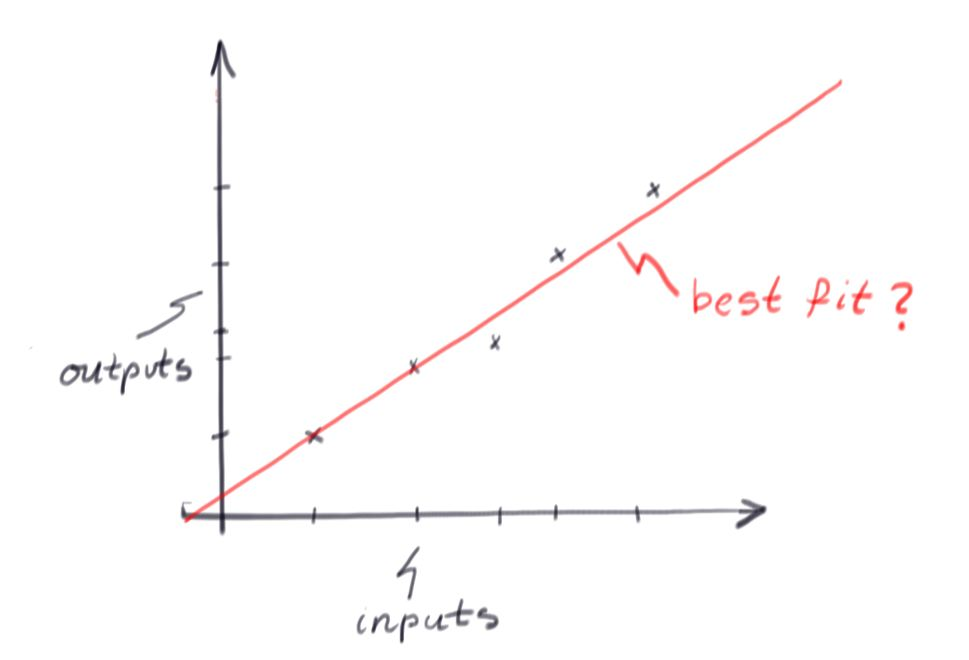
\includegraphics[scale=.2]{best_fit.jpg}
\end{center}

In equation~\eqref{linsys} we have $n$ {\it linear} functions called $f_1,\ldots, f_n$, $m$ un\-knowns $x_1,\ldots, x_m$
and $n$ given constants $a_1,\ldots,a_n$. We need to say what it means for a function to be linear.
A linear function has the {\it additive property}
$$
f(a+b)=f(a)+f(b)\, .
$$
The solution to this is
$$
f(x)=\lambda x\, ,
$$
for some constant $\lambda$. The plot of this is just a straight line through the origin with 
slope~$\lambda$
\begin{center}
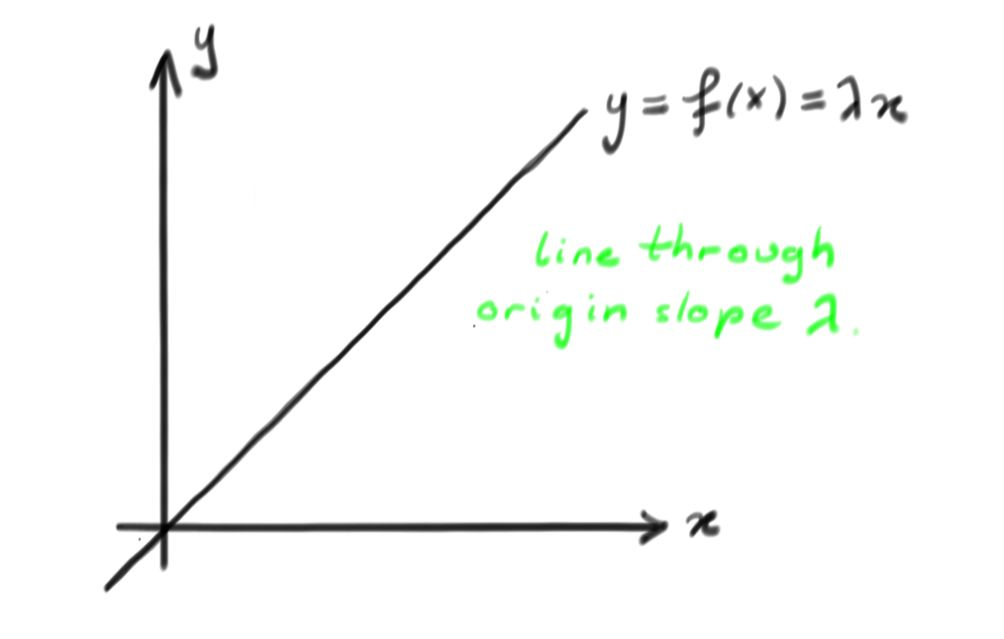
\includegraphics[scale=.2]{line_through_origin.jpg}
\end{center}

We should also check that our solution obeys the linearity property. The logic is to start with the left hand side $f(a+b)$
and try to turn it into the right hand side $f(a)+f(b)$ using correct manipulations:
$$
f(a+b)=\lambda(a+b) =\lambda a + \lambda b = f(a) + f(b)\, .
$$
The first step here just plugs $a+b$ into $f(x)$, the second is the distributive property, and in the third we recognize that $\lambda a = f(a)$ and $\lambda b = f(b)$.
This proves our claim.

For functions of many variables, linearity must hold for every slot. For a linear function of two variables $f(x,y)$ this means
$$
f(a+b,c+d)=f(a,c)+f(b,d)\, .
$$

We finish with a question. The plot of $f(x)=\lambda x + \beta$ is a straight line, but does it obey the linearity property?

%%%%don't forget to close the bracket so the stuff after your file doesn't look like a movie!
}

\newpage

%
%
%
\subsection{\whatIsTitle: $3 \times 3$ Matrix Example}

{\ttfamily
\fontdimen2\font=0.4em
\fontdimen3\font=0.2em
\fontdimen4\font=0.1em
\fontdimen7\font=0.1em
\hyphenchar\font=`\-

\hypertarget{scripts_what_is_linear_algebra_3_3_matrix}{Your friend places a jar} on a table and tells you that there is 65 cents in this jar with 7 coins consisting of quarters, nickels, and dimes, and that there are twice as many dimes as quarters. Your friend wants to know how many nickels, dimes, and quarters are in the jar.

We can translate this into a system of the following linear equations:
\begin{align*}
5n + 10d + 25q & = 65
\\ n + d + q & = 7
\\ d & = 2q
\end{align*}
Now we can rewrite the last equation in the form of $-d + 2q = 0$, and thus express this problem as the matrix equation
\[
\begin{pmatrix}
5 & 10 & 25 \\
1 & 1 & 1 \\
0 & -1 & 2
\end{pmatrix} \begin{pmatrix}n\\d\\q\end{pmatrix} = \begin{pmatrix}65\\7\\0\end{pmatrix}.
\]
or as an \hyperlink{augmented_matrix}{augmented matrix} (see also \hyperlink{script_gaussian_elimination_more}{this script on the notation}).
\[
\begin{pmatrix}
5 & 10 & 25 & \vline & 65\\
1 & 1 & 1 & \vline & 7 \\
0 & -1 & 2 & \vline & 0
\end{pmatrix}
\]
Now to solve it, using our original set of equations and by substitution, we have
\begin{align*}
5n + 20q + 25q = 5n + 45q & = 65
\\ n + 2q + q = n + 3q & = 7
\end{align*}
and by subtracting 5 times the bottom equation from the top, we get
\[
45q - 15q = 30q = 65 - 35 = 30
\]
and hence $q = 1$. Clearly $d = 2$, and hence $n = 7 - 2 - 1 = 4$. Therefore there are four nickels, two dimes, and one quarter.

} % Closing brace for font

\newpage

%

\subsection*{Hint for Review  Question~\ref{orthogprob}}

%%%Insert this to get the typewriter font so it looks like a real movie script
{\ttfamily
\fontdimen2\font=0.4em
\fontdimen3\font=0.2em
\fontdimen4\font=0.1em
\fontdimen7\font=0.1em
\hyphenchar\font=`\-


You are asked to consider an orthogonal basis $\{v_1,v_2,\ldots v_n\}$.
Because this is a basis any $v\in V$ can be uniquely expressed as
$$
v=c^1 v_1 + c^2 v_2 +\cdots +v^n c_n\, ,
$$
and the number $n=\dim V$. Since this is an orthogonal basis
$$
v_i\dotprod v_j =0 \, ,\qquad i\neq j\, .
$$
So different vectors in the basis are orthogonal:
\begin{center}
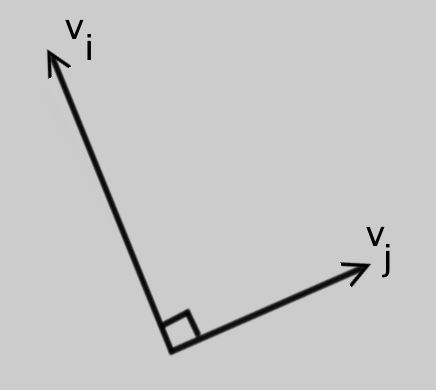
\includegraphics[scale=.4]{\orthonormPath/rightangles.jpg}
\end{center}
However, the basis is {\it not} orthonormal so we know nothing about the
lengths of the basis vectors (save that they cannot vanish). 

To complete the hint, lets use the dot product to compute a formula for $c^1$ in terms of the basis vectors and $v$. Consider
$$
v_1\dotprod v = c^1 v_1\dotprod v_1 + c^2 v_1\dotprod v^2 +\cdots + c^n v_1\dotprod v_n=c^1 v_1\dotprod v_1\, .
$$
Solving for $c^1$ (remembering that $v_1\dotprod v_1\neq 0$) gives
$$
c^1 = \frac{v_1\dotprod v\ }{v_1\dotprod v_1}\, .
$$
This should get you started on this problem.

} % Closing bracket for font

%\newpage

%%Hint for Pablo's fruit and barrel conundrum
%
\section{Systems of Linear Equations}

%\subsection*{\gaussElimTitle: Augmented Matrix Notation}
\subsection*{Augmented Matrix Notation}

%%%Insert this to get the typewriter font so it looks like a real movie script
{\ttfamily
\fontdimen2\font=0.4em
\fontdimen3\font=0.2em
\fontdimen4\font=0.1em
\fontdimen7\font=0.1em
\hyphenchar\font=`\-


%%%%put a hypertarget around the opening bit of text
\hypertarget{script_gaussian_elimination_more}{Why is the augmented  matrix} 
$$ \left( \begin{array}{cc | c}
1 & 1 & 27 \\
2 & -1 & 0  
\end{array} \right)\, ,
$$
equivalent to the system of equations
\begin{eqnarray*}
 x+y &=& 27\\
 2x - y &=& 0\, ?
\end{eqnarray*}
Well the augmented matrix is just a new notation for the matrix equation
\begin{equation*}
    \begin{pmatrix}
      1             &1  \\
      2             &-1
    \end{pmatrix}
  \colvec{x \\ y}
  =
  \colvec{27 \\ 0}
\end{equation*}
and if you review your matrix multiplication remember that 
\begin{equation*}
    \begin{pmatrix}
      1             &1  \\
      2             &-1
    \end{pmatrix}
  \colvec{x \\ y}
  =
  \colvec{x+ y \\ 2x - y}
\end{equation*}
This means that

\begin{equation*}
  \colvec{x+ y \\ 2x - y}
  =
  \colvec{27 \\ 0}\, ,
\end{equation*}
which is our original equation.

%%%%don't forget to close the bracket so the stuff after your file doesn't look like a movie!
}


%
\subsection*{Equivalence of Augmented Matrices}

%%%Insert this to get the typewriter font so it looks like a real movie script
{\ttfamily
\fontdimen2\font=0.4em
\fontdimen3\font=0.2em
\fontdimen4\font=0.1em
\fontdimen7\font=0.1em
\hyphenchar\font=`\-


%%%%put a hypertarget around the opening bit of text
\hypertarget{script_gaussian_elimination_background}{Lets think about what it means for the two augmented matrices} 


$$ \left( \begin{array}{cc | c}
1 & 1 & 27 \\
2 & -1 & 0  
\end{array} \right)
\mbox{ and } \left( \begin{array}{cc | c}
1 & 0 & 9 \\
0 & 1 & 18  
\end{array} \right)
$$
to be equivalent:
They are certainly not equal, because they don't match in each component, but since these augmented matrices represent a system, we might want to introduce a new kind of equivalence relation.

Well we could look at the system of linear equations this represents 

\begin{eqnarray*}
 x+y &=& 27\\
 2x - y &=& 0\, 
\end{eqnarray*}
and notice that the solution is $x=9$ and $y=18$. The other augmented matrix represents the system 
\begin{eqnarray*}
 x\ +0 \cdot y &=& 9\\
 0 \cdot x \ +\   \phantom{0 \cdot} y  &=& 18\, 
\end{eqnarray*}
This clearly has the same solution. The first and second system are related in the sense that their solutions are the same. Notice that it is really nice to have the augmented matrix in the second form, because the matrix multiplication can be done in your head.


%%%%don't forget to close the bracket so the stuff after your file doesn't look like a movie!
}

%\newpage
%

\subsection*{Hint for Review  Question~\ref{orthogprob}}

%%%Insert this to get the typewriter font so it looks like a real movie script
{\ttfamily
\fontdimen2\font=0.4em
\fontdimen3\font=0.2em
\fontdimen4\font=0.1em
\fontdimen7\font=0.1em
\hyphenchar\font=`\-


You are asked to consider an orthogonal basis $\{v_1,v_2,\ldots v_n\}$.
Because this is a basis any $v\in V$ can be uniquely expressed as
$$
v=c^1 v_1 + c^2 v_2 +\cdots +v^n c_n\, ,
$$
and the number $n=\dim V$. Since this is an orthogonal basis
$$
v_i\dotprod v_j =0 \, ,\qquad i\neq j\, .
$$
So different vectors in the basis are orthogonal:
\begin{center}
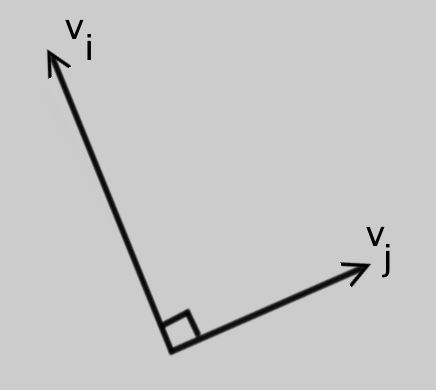
\includegraphics[scale=.4]{\orthonormPath/rightangles.jpg}
\end{center}
However, the basis is {\it not} orthonormal so we know nothing about the
lengths of the basis vectors (save that they cannot vanish). 

To complete the hint, lets use the dot product to compute a formula for $c^1$ in terms of the basis vectors and $v$. Consider
$$
v_1\dotprod v = c^1 v_1\dotprod v_1 + c^2 v_1\dotprod v^2 +\cdots + c^n v_1\dotprod v_n=c^1 v_1\dotprod v_1\, .
$$
Solving for $c^1$ (remembering that $v_1\dotprod v_1\neq 0$) gives
$$
c^1 = \frac{v_1\dotprod v\ }{v_1\dotprod v_1}\, .
$$
This should get you started on this problem.

} % Closing bracket for font

%\newpage

%
%
\subsection{\gaussElimTitle: $3 \times 3$ Example}

{\ttfamily
\fontdimen2\font=0.4em
\fontdimen3\font=0.2em
\fontdimen4\font=0.1em
\fontdimen7\font=0.1em
\hyphenchar\font=`\-

\hypertarget{scripts_gaussian_elimination_3_3_example}{We'll start with the matrix} from the \hyperlink{scripts_what_is_linear_algebra_3_3_matrix}{What is Linear Algebra: $3 \times 3$ Matrix Example} which was
\[
\begin{pmatrix}
5 & 10 & 25 & \vline & 65\\
1 & 1 & 1 & \vline & 7 \\
0 & -1 & 2 & \vline & 0
\end{pmatrix},
\]
and recall the solution to the problem was $n = 4$, $d = 2$, and $q = 1$. So as a matrix equation we have
\[
\begin{pmatrix}1 & 0 & 0 \\ 0 & 1 & 0 \\ 0 & 0 & 1\end{pmatrix} \begin{pmatrix}n \\ d \\ q\end{pmatrix} = \begin{pmatrix}4 \\ 2 \\ 1 \end{pmatrix}
\]
or as an augmented matrix
\[
\begin{pmatrix}
1 & & & \vline & 4 \\
& 1 & & \vline & 2 \\
& & 1 & \vline & 1
\end{pmatrix}
\]

Note that often in diagonal matrices people will either omit the zeros or write in a single large zero. Now
the first matrix is equivalent to the second matrix and is written as
\[
\begin{pmatrix}
5 & 10 & 25 & \vline & 65\\
1 & 1 & 1 & \vline & 7 \\
0 & -1 & 2 & \vline & 0
\end{pmatrix},
\sim
\begin{pmatrix}
1 & & & \vline & 4 \\
& 1 & & \vline & 2 \\
& & 1 & \vline & 1
\end{pmatrix}
\]
since they have the same solutions.


} % Closing brace for the font

\newpage

%
%
\subsection*{Worked Example}

%%%Insert this to get the typewriter font so it looks like a real movie script
{\ttfamily
\fontdimen2\font=0.4em
\fontdimen3\font=0.2em
\fontdimen4\font=0.1em
\fontdimen7\font=0.1em
\hyphenchar\font=`\-


\hypertarget{basis_and_dimension_example}{In this} 
video we will work through an example of how to extend a set of linearly independent vectors to a basis. For fun, we will take
the vector space 
$$
V=\{(x,y,z,w)|x,y,z,w\in {\mathbb Z}^5\}\, .
$$
This is like four dimensional space ${\mathbb R}^4$ except that the numbers can only be $\{0,1,2,3,4\}$. This is like bits, but now the rule is
$$
0=5\, .
$$
Thus, for example,  $\frac14=4$ because $4\time 4=16=1+3\times 5=1$. Don't get too caught up on this aspect, its a choice of base field designed
to make computations go quicker!

Now, here's the problem we will solve:

\begin{center}
{\bf Find a basis for $V$ that includes the vectors $\begin{pmatrix}1\\2\\3\\4\end{pmatrix}$ and $\begin{pmatrix}0\\3\\2\\1\end{pmatrix}$.}
\end{center}

The way to proceed is to add a known (and preferably simple) basis to the vectors given, thus we consider
\[
v_1=\begin{pmatrix}1\\2\\3\\4\end{pmatrix},\
v_2=\begin{pmatrix}0\\3\\2\\1\end{pmatrix},\
e_1=\begin{pmatrix}1\\0\\0\\0\end{pmatrix},\
e_2=\begin{pmatrix}0\\1\\0\\0\end{pmatrix},\
e_3=\begin{pmatrix}0\\0\\1\\0\end{pmatrix},\
e_4=\begin{pmatrix}0\\0\\0\\1\end{pmatrix}.
\]
The last four vectors are clearly a basis (make sure you understand this....) and are called the {\it canonical basis}\index{Canonical basis}.
We want to keep $v_1$ and $v_2$ but find a way to turf out two of the vectors in the canonical basis leaving us
a basis of four vectors. To do that, we have to study linear independence, or in other words a linear system problem
defined by
$$
0=\alpha_1 e_1 + \alpha_2 e_2 + \alpha_3 v_1 + \alpha_4 v_2 + \alpha_5 e_3 + \alpha_6 e_4 \, .
$$
We want to find solutions for the $\alpha's$ which allow us to determine two of the $e's$.
For that we use an augmented matrix
$$
\left(\begin{array}{cccccc|c}
1&0&1&0&0&0&0\\
2&3&0&1&0&0&0\\
3&2&0&0&1&0&0\\
4&1&0&0&0&1&0
\end{array}\right)\, .
$$
Next comes a bunch of row operations. Note that we have dropped the last column of zeros since it has no information--you can fill in the 
row operations used above the $\sim$'s as an exercise:
$$
\begin{pmatrix}
1&0&1&0&0&0\\
2&3&0&1&0&0\\
3&2&0&0&1&0\\
4&1&0&0&0&1
\end{pmatrix}\sim
\begin{pmatrix}
1&0&1&0&0&0\\
0&3&3&1&0&0\\
0&2&2&0&1&0\\
0&1&1&0&0&1
\end{pmatrix}
$$
$$
\sim
\begin{pmatrix}
1&0&1&0&0&0\\
0&1&1&2&0&0\\
0&2&2&0&1&0\\
0&1&1&0&0&1
\end{pmatrix}
\sim
\begin{pmatrix}
1&0&1&0&0&0\\
0&1&1&2&0&0\\
0&0&0&1&1&0\\
0&0&0&3&0&1
\end{pmatrix}
$$
$$
\sim
\begin{pmatrix}
1&0&1&0&0&0\\
0&1&1&0&3&0\\
0&0&0&1&1&0\\
0&0&0&0&2&1
\end{pmatrix}
\sim
\begin{pmatrix}
1&0&1&0&0&0\\
0&1&1&0&3&0\\
0&0&0&1&1&0\\
0&0&0&0&1&3
\end{pmatrix}
$$
$$
\sim
\begin{pmatrix}
\underline1&0&1&0&0&0\\
0&\underline1&1&0&0&1\\
0&0&0&\underline1&0&2\\
0&0&0&0&\underline1&3
\end{pmatrix}
$$
The pivots are underlined.
The columns corresponding to non-pivot variables are the ones that can be eliminated--their coefficients (the $\alpha$'s)
will be arbitrary, so set them all to zero save for the one next to the vector you are solving for which can be taken to be unity.
Thus that vector can certainly be expressed in terms of previous ones. Hence, altogether, our basis is
$$
\left\{
\begin{pmatrix}1\\2\\3\\4\end{pmatrix} \, , \ 
\begin{pmatrix}0\\3\\2\\1\end{pmatrix} ,\
\begin{pmatrix}0\\1\\0\\0\end{pmatrix} ,\
\begin{pmatrix}0\\0\\1\\0\end{pmatrix}
\right\}\, .
$$
Finally, as a check, note that $e_1=v_1+v_2$ which explains why we had to throw it away.



} % Closing bracket for font

%\newpage

%

\subsection*{Worked Example}

%%%Insert this to get the typewriter font so it looks like a real movie script
{\ttfamily
\fontdimen2\font=0.4em
\fontdimen3\font=0.2em
\fontdimen4\font=0.1em
\fontdimen7\font=0.1em
\hyphenchar\font=`\-


\hypertarget{basis_and_dimension_example}{In this} 
video we will work through an example of how to extend a set of linearly independent vectors to a basis. For fun, we will take
the vector space 
$$
V=\{(x,y,z,w)|x,y,z,w\in {\mathbb Z}^5\}\, .
$$
This is like four dimensional space ${\mathbb R}^4$ except that the numbers can only be $\{0,1,2,3,4\}$. This is like bits, but now the rule is
$$
0=5\, .
$$
Thus, for example,  $\frac14=4$ because $4\time 4=16=1+3\times 5=1$. Don't get too caught up on this aspect, its a choice of base field designed
to make computations go quicker!

Now, here's the problem we will solve:

\begin{center}
{\bf Find a basis for $V$ that includes the vectors $\begin{pmatrix}1\\2\\3\\4\end{pmatrix}$ and $\begin{pmatrix}0\\3\\2\\1\end{pmatrix}$.}
\end{center}

The way to proceed is to add a known (and preferably simple) basis to the vectors given, thus we consider
\[
v_1=\begin{pmatrix}1\\2\\3\\4\end{pmatrix},\
v_2=\begin{pmatrix}0\\3\\2\\1\end{pmatrix},\
e_1=\begin{pmatrix}1\\0\\0\\0\end{pmatrix},\
e_2=\begin{pmatrix}0\\1\\0\\0\end{pmatrix},\
e_3=\begin{pmatrix}0\\0\\1\\0\end{pmatrix},\
e_4=\begin{pmatrix}0\\0\\0\\1\end{pmatrix}.
\]
The last four vectors are clearly a basis (make sure you understand this....) and are called the {\it canonical basis}\index{Canonical basis}.
We want to keep $v_1$ and $v_2$ but find a way to turf out two of the vectors in the canonical basis leaving us
a basis of four vectors. To do that, we have to study linear independence, or in other words a linear system problem
defined by
$$
0=\alpha_1 e_1 + \alpha_2 e_2 + \alpha_3 v_1 + \alpha_4 v_2 + \alpha_5 e_3 + \alpha_6 e_4 \, .
$$
We want to find solutions for the $\alpha's$ which allow us to determine two of the $e's$.
For that we use an augmented matrix
$$
\left(\begin{array}{cccccc|c}
1&0&1&0&0&0&0\\
2&3&0&1&0&0&0\\
3&2&0&0&1&0&0\\
4&1&0&0&0&1&0
\end{array}\right)\, .
$$
Next comes a bunch of row operations. Note that we have dropped the last column of zeros since it has no information--you can fill in the 
row operations used above the $\sim$'s as an exercise:
$$
\begin{pmatrix}
1&0&1&0&0&0\\
2&3&0&1&0&0\\
3&2&0&0&1&0\\
4&1&0&0&0&1
\end{pmatrix}\sim
\begin{pmatrix}
1&0&1&0&0&0\\
0&3&3&1&0&0\\
0&2&2&0&1&0\\
0&1&1&0&0&1
\end{pmatrix}
$$
$$
\sim
\begin{pmatrix}
1&0&1&0&0&0\\
0&1&1&2&0&0\\
0&2&2&0&1&0\\
0&1&1&0&0&1
\end{pmatrix}
\sim
\begin{pmatrix}
1&0&1&0&0&0\\
0&1&1&2&0&0\\
0&0&0&1&1&0\\
0&0&0&3&0&1
\end{pmatrix}
$$
$$
\sim
\begin{pmatrix}
1&0&1&0&0&0\\
0&1&1&0&3&0\\
0&0&0&1&1&0\\
0&0&0&0&2&1
\end{pmatrix}
\sim
\begin{pmatrix}
1&0&1&0&0&0\\
0&1&1&0&3&0\\
0&0&0&1&1&0\\
0&0&0&0&1&3
\end{pmatrix}
$$
$$
\sim
\begin{pmatrix}
\underline1&0&1&0&0&0\\
0&\underline1&1&0&0&1\\
0&0&0&\underline1&0&2\\
0&0&0&0&\underline1&3
\end{pmatrix}
$$
The pivots are underlined.
The columns corresponding to non-pivot variables are the ones that can be eliminated--their coefficients (the $\alpha$'s)
will be arbitrary, so set them all to zero save for the one next to the vector you are solving for which can be taken to be unity.
Thus that vector can certainly be expressed in terms of previous ones. Hence, altogether, our basis is
$$
\left\{
\begin{pmatrix}1\\2\\3\\4\end{pmatrix} \, , \ 
\begin{pmatrix}0\\3\\2\\1\end{pmatrix} ,\
\begin{pmatrix}0\\1\\0\\0\end{pmatrix} ,\
\begin{pmatrix}0\\0\\1\\0\end{pmatrix}
\right\}\, .
$$
Finally, as a check, note that $e_1=v_1+v_2$ which explains why we had to throw it away.



} % Closing bracket for font

%\newpage



\subsection*{Worked Examples of Gaussian Elimination}

{\ttfamily
\fontdimen2\font=0.4em
\fontdimen3\font=0.2em
\fontdimen4\font=0.1em
\fontdimen7\font=0.1em
\hyphenchar\font=`\-

\hypertarget{scripts_elementary_row_operations_worked_examples}{Let us consider that we are} given two systems of equations that give rise to the following two (augmented) matrices:
\begin{align*}
\begin{pmatrix}
2 & 5 & 2 & 0 & \vline & 2 \\
1 & 1 & 1 & 0 & \vline & 1 \\
1 & 4 & 1 & 0 & \vline & 1
\end{pmatrix}
\quad\quad
\begin{pmatrix}
5 & 2 & \vline & 9 \\
0 & 5 & \vline & 10 \\
0 & 3 & \vline & 6
\end{pmatrix}
\end{align*}
and we want to find the solution to those systems. We will do so by doing Gaussian elimination.

For the first matrix we have
\begin{align*}
\begin{pmatrix}
2 & 5 & 2 & 0 & \vline & 2 \\
1 & 1 & 1 & 0 & \vline & 1 \\
1 & 4 & 1 & 0 & \vline & 1
\end{pmatrix}
\overset{R_1 \leftrightarrow R_2}{\sim} &
\begin{pmatrix}
1 & 1 & 1 & 0 & \vline & 1 \\
2 & 5 & 2 & 0 & \vline & 2 \\
1 & 4 & 1 & 0 & \vline & 1
\end{pmatrix}
\\ \overset{R_2 - 2 R_1 ; R_3 - R_1}{\sim} &
\begin{pmatrix}
1 & 1 & 1 & 0 & \vline & 1 \\
0 & 3 & 0 & 0 & \vline & 0 \\
0 & 3 & 0 & 0 & \vline & 0
\end{pmatrix}
\\ \overset{\frac{1}{3}R_2}{\sim} &
\begin{pmatrix}
1 & 1 & 1 & 0 & \vline & 1 \\
0 & 1 & 0 & 0 & \vline & 0 \\
0 & 3 & 0 & 0 & \vline & 0
\end{pmatrix}
\\ \overset{R_1 - R_2 ; R_3 - 3 R_2}{\sim} &
\begin{pmatrix}
1 & 0 & 1 & 0 & \vline & 1 \\
0 & 1 & 0 & 0 & \vline & 0 \\
0 & 0 & 0 & 0 & \vline & 0
\end{pmatrix}
\end{align*}
\begin{enumerate}[1.]
\item We begin by interchanging the first two rows in order to get a 1 in the upper-left hand corner and avoiding dealing with fractions.

\item Next we subtract row 1 from row 3 and twice from row 2 to get zeros in the left-most column.

\item Then we scale row 2 to have a 1 in the eventual pivot.

\item Finally we subtract row 2 from row 1 and three times from row 2 to get it into Reduced Row  Echelon Form.
\end{enumerate}
Therefore we can write $x = 1 - \lambda$, $y = 0$, $z = \lambda$ and $w = \mu$, or in vector form
\[
\begin{pmatrix}x\\y\\z\\w\end{pmatrix} = \begin{pmatrix}1\\0\\0\\0\end{pmatrix} + \lambda \begin{pmatrix}-1\\0\\1\\0\end{pmatrix} + \mu \begin{pmatrix}0\\0\\0\\1\end{pmatrix}.
\]

Now for the second system we have
\begin{align*}
\begin{pmatrix}
5 & 2 & \vline & 9 \\
0 & 5 & \vline & 10 \\
0 & 3 & \vline & 6
\end{pmatrix}
\overset{\frac{1}{5}R_2}{\sim} &
\begin{pmatrix}
5 & 2 & \vline & 9 \\
0 & 1 & \vline & 2 \\
0 & 3 & \vline & 6
\end{pmatrix}
\\ \overset{R_3 - 3 R_2}{\sim} &
\begin{pmatrix}
5 & 2 & \vline & 9 \\
0 & 1 & \vline & 2 \\
0 & 0 & \vline & 0
\end{pmatrix}
\\ \overset{R_1 - 2 R_2}{\sim} &
\begin{pmatrix}
5 & 0 & \vline & 5 \\
0 & 1 & \vline & 2 \\
0 & 0 & \vline & 0
\end{pmatrix}
\\ \overset{\frac{1}{5}R_1}{\sim} &
\begin{pmatrix}
1 & 0 & \vline & 1 \\
0 & 1 & \vline & 2 \\
0 & 0 & \vline & 0
\end{pmatrix}
\end{align*}
We scale the second and third rows appropriately in order to avoid fractions, then subtract the corresponding rows as before. Finally scale the first row and hence we have $x = 1$ and $y = 2$ as a unique solution.

} % Closing brace for the font

%\newpage

%
%
\subsection{\elemRowOpsTitle: Explanation of Proof for Theorem~\ref{GJEunique}}

{\ttfamily
\fontdimen2\font=0.4em
\fontdimen3\font=0.2em
\fontdimen4\font=0.1em
\fontdimen7\font=0.1em
\hyphenchar\font=`\-

\hypertarget{scripts_elementary_row_operations_proof}{The first thing to realize is that} 
there are choices in the Gaussian elimination recipe, so maybe that could lead to two different
RREF's and in turn two different solution sets for the same linear system. But that would be weird,
in fact this Theorem says that this can never happen!

Because this proof comes at the end of the section it is often glossed over, but it is a very important result.
Here's a sketch of what happens in the video:
\begin{center}
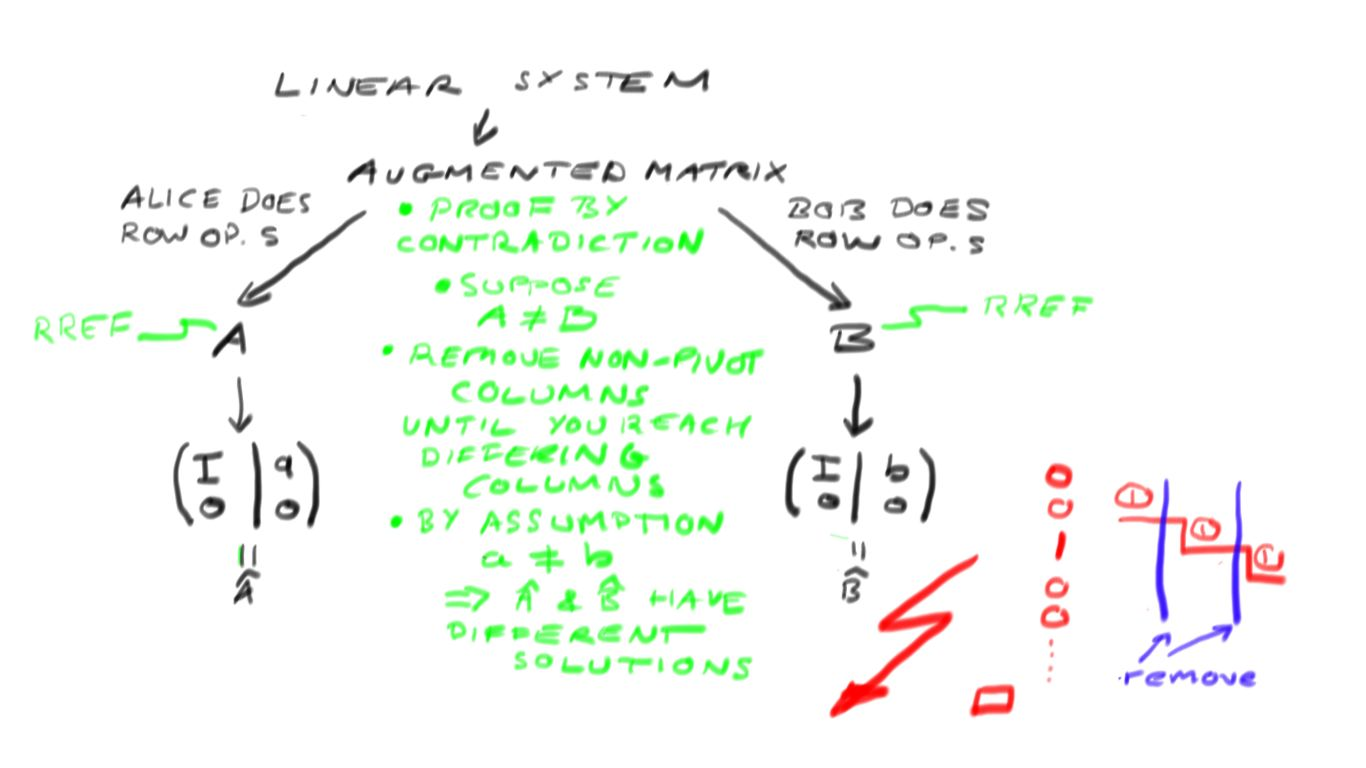
\includegraphics[scale=.3]{RREF_unique.jpg}
\end{center}

In words: we start with a linear system and convert it to an augmented matrix. Then, because we are studying a uniqueness
statement, we try a proof by contradiction. That is the  method where to show that a statement is true, you try to demonstrate that
the opposite of the statement leads to a contradiction. Here, the opposite statement to the theorem would be to find
two different RREFs for the same system.

Suppose, therefore, that Alice and Bob do find different RREF augmented matrices called $A$ and $B$. 
Then remove all the non-pivot columns  from $A$ and $B$  until you hit the first column that differs. Record that in the last column
and call the results $\widehat A$ and $\widehat B$. Removing columns
does change the solution sets, but it does not ruin row equivalence, so  $\widehat A$ and $\widehat B$ have the same solution sets.

Now, because we left only the pivot columns (plus the first column that differs) we have
$$\hat{A}=\begin{amatrix}{1}
I_N & a\\
0 & 0
\end{amatrix} \mbox{ and } \hat{B}=\begin{amatrix}{1}
I_N & b\\
0 & 0
\end{amatrix}\, ,$$ where $I_N$ is an identity matrix and $a$ and $b$ are column vectors.
Importantly, by assumption,
$$
a\neq b\, .
$$
So if we try to wrote down the solution sets for $\widehat A$ and $\widehat B$ they would be different.
But at all stages, we only performed operations that kept Alice's solution set the same as Bob's.
This is a contradiction so the proof is complete.
} % Closing brace for the font

\newpage

%

\subsection*{Hint for Review  Question~\ref{orthogprob}}

%%%Insert this to get the typewriter font so it looks like a real movie script
{\ttfamily
\fontdimen2\font=0.4em
\fontdimen3\font=0.2em
\fontdimen4\font=0.1em
\fontdimen7\font=0.1em
\hyphenchar\font=`\-


You are asked to consider an orthogonal basis $\{v_1,v_2,\ldots v_n\}$.
Because this is a basis any $v\in V$ can be uniquely expressed as
$$
v=c^1 v_1 + c^2 v_2 +\cdots +v^n c_n\, ,
$$
and the number $n=\dim V$. Since this is an orthogonal basis
$$
v_i\dotprod v_j =0 \, ,\qquad i\neq j\, .
$$
So different vectors in the basis are orthogonal:
\begin{center}
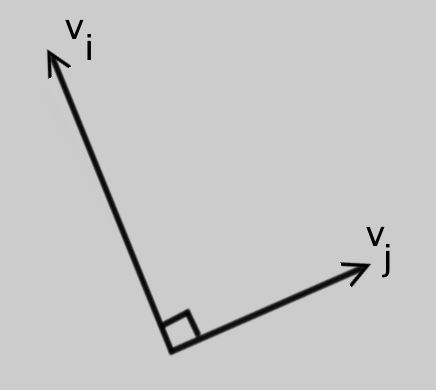
\includegraphics[scale=.4]{\orthonormPath/rightangles.jpg}
\end{center}
However, the basis is {\it not} orthonormal so we know nothing about the
lengths of the basis vectors (save that they cannot vanish). 

To complete the hint, lets use the dot product to compute a formula for $c^1$ in terms of the basis vectors and $v$. Consider
$$
v_1\dotprod v = c^1 v_1\dotprod v_1 + c^2 v_1\dotprod v^2 +\cdots + c^n v_1\dotprod v_n=c^1 v_1\dotprod v_1\, .
$$
Solving for $c^1$ (remembering that $v_1\dotprod v_1\neq 0$) gives
$$
c^1 = \frac{v_1\dotprod v\ }{v_1\dotprod v_1}\, .
$$
This should get you started on this problem.

} % Closing bracket for font

%\newpage


\subsection*{Hint for Review  Question~\ref{orthogprob}}

%%%Insert this to get the typewriter font so it looks like a real movie script
{\ttfamily
\fontdimen2\font=0.4em
\fontdimen3\font=0.2em
\fontdimen4\font=0.1em
\fontdimen7\font=0.1em
\hyphenchar\font=`\-


You are asked to consider an orthogonal basis $\{v_1,v_2,\ldots v_n\}$.
Because this is a basis any $v\in V$ can be uniquely expressed as
$$
v=c^1 v_1 + c^2 v_2 +\cdots +v^n c_n\, ,
$$
and the number $n=\dim V$. Since this is an orthogonal basis
$$
v_i\dotprod v_j =0 \, ,\qquad i\neq j\, .
$$
So different vectors in the basis are orthogonal:
\begin{center}
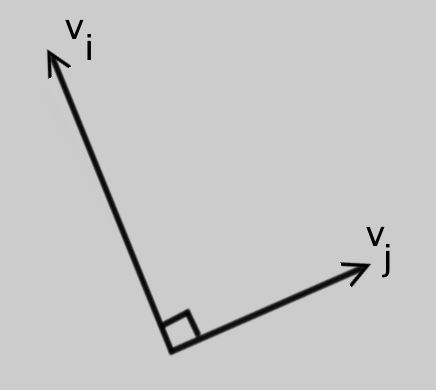
\includegraphics[scale=.4]{\orthonormPath/rightangles.jpg}
\end{center}
However, the basis is {\it not} orthonormal so we know nothing about the
lengths of the basis vectors (save that they cannot vanish). 

To complete the hint, lets use the dot product to compute a formula for $c^1$ in terms of the basis vectors and $v$. Consider
$$
v_1\dotprod v = c^1 v_1\dotprod v_1 + c^2 v_1\dotprod v^2 +\cdots + c^n v_1\dotprod v_n=c^1 v_1\dotprod v_1\, .
$$
Solving for $c^1$ (remembering that $v_1\dotprod v_1\neq 0$) gives
$$
c^1 = \frac{v_1\dotprod v\ }{v_1\dotprod v_1}\, .
$$
This should get you started on this problem.

} % Closing bracket for font

%\newpage

%

\subsection*{Planes}

%%%Insert this to get the typewriter font so it looks like a real movie script
{\ttfamily
\fontdimen2\font=0.4em
\fontdimen3\font=0.2em
\fontdimen4\font=0.1em
\fontdimen7\font=0.1em
\hyphenchar\font=`\-


%%%%put a hypertarget around the opening bit of text
\hypertarget{solution_sets_for_systems_of_linear_equations_planes}{Here we want} to describe the mathematics of planes in space.
The video is summarised by the following picture:
\begin{center}
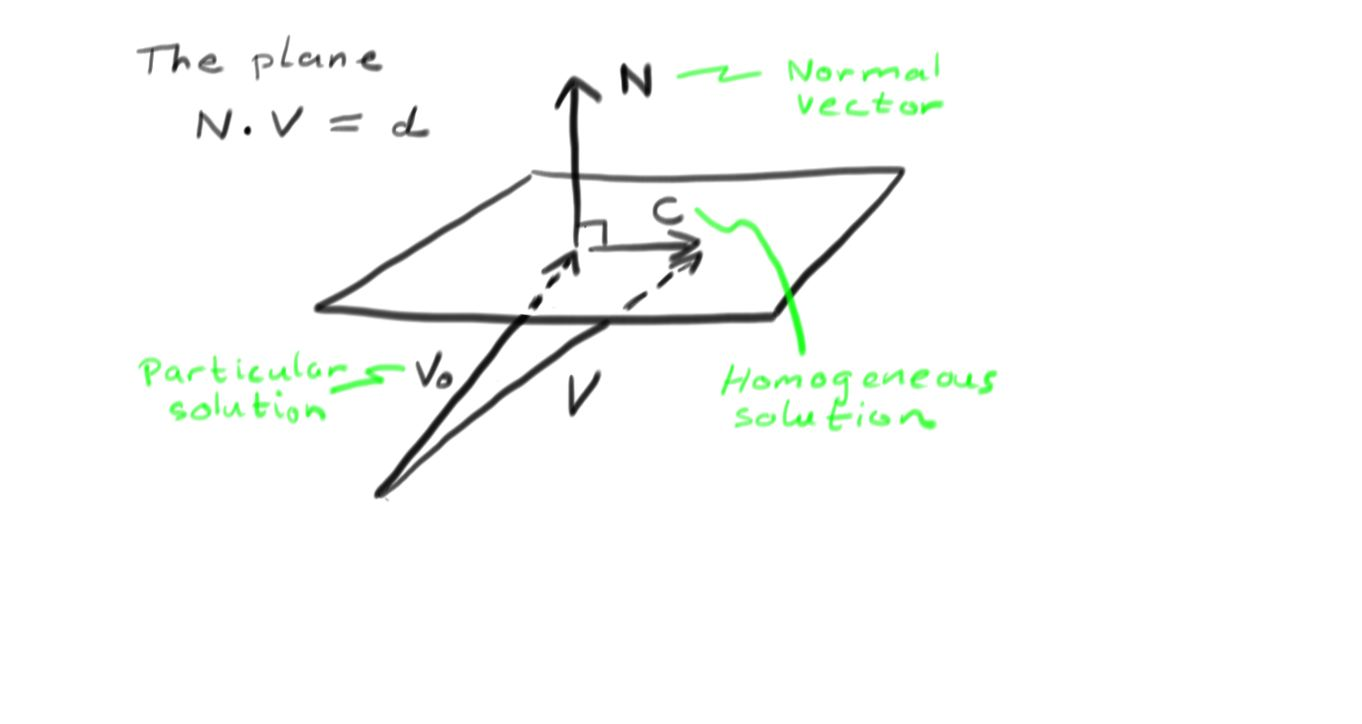
\includegraphics[scale=.2]{plane1eq.jpg}
\end{center}
A plane is often called ${\mathbb R}^2$ because it is spanned by  two coordinates, and space is called ${\mathbb R}^3$ and has three coordinates, 
usually called $(x,y,z)$. The equation for a plane is
$$
ax+by+cz=d\, .
$$
Lets simplify this by calling $V=(x,y,z)$ the vector of unknowns and $N=(a,b,c)$. Using the dot product in ${\mathbb R}^3$
we have
$$
N\dotprod V = d\, .
$$
Remember that when vectors are perpendicular their dot products vanish. {\it I.e.} $U\dotprod V = 0 \Leftrightarrow U \perp V$.
This means that if a vector $V_0$ solves our equation $N\dotprod V =d$, then so too does $V_0+C$ whenever $C$ is perpendicular to $N$.
This is because
$$N\dotprod (V_0+C) = N\dotprod V_0 + N\dotprod C = d + 0 = d\, .$$
But $C$ is ANY vector perpendicular to $N$, so all the possibilities for $C$ span a plane whose normal vector is $N$. Hence we have shown that 
solutions to the equation $ax+by+cz=0$ are a plane with normal vector $N=(a,b,c)$.



%%%%don't forget to close the bracket so the stuff after your file doesn't look like a movie!
}

%\newpage

%

\subsection{\whatIsTitle: Overview}

%%%Insert this to get the typewriter font so it looks like a real movie script
{\ttfamily
\fontdimen2\font=0.4em
\fontdimen3\font=0.2em
\fontdimen4\font=0.1em
\fontdimen7\font=0.1em
\hyphenchar\font=`\-


%%%%put a hypertarget around the opening bit of text
\hypertarget{video_what_is_overview}{In this course, we start with linear systems} 
\begin{equation}\label{linsys}
\left\{
\begin{array}{ccc}
f_1(x_1,\ldots,x_m)& = &a_1\\[1mm]
\vdots&&\vdots\\[1mm]
f_n(x_1,\ldots,x_m) &=& a_n\, ,
\end{array}
\right.
\end{equation}
and discuss how to solve them.

We end with the problem of finding a least squares fit---find the line that best fits a given data set:
\begin{center}
\includegraphics[scale=.2]{best_fit.jpg}
\end{center}

In equation~\eqref{linsys} we have $n$ {\it linear} functions called $f_1,\ldots, f_n$, $m$ un\-knowns $x_1,\ldots, x_m$
and $n$ given constants $a_1,\ldots,a_n$. We need to say what it means for a function to be linear.
A linear function has the {\it additive property}
$$
f(a+b)=f(a)+f(b)\, .
$$
The solution to this is
$$
f(x)=\lambda x\, ,
$$
for some constant $\lambda$. The plot of this is just a straight line through the origin with 
slope~$\lambda$
\begin{center}
\includegraphics[scale=.2]{line_through_origin.jpg}
\end{center}

We should also check that our solution obeys the linearity property. The logic is to start with the left hand side $f(a+b)$
and try to turn it into the right hand side $f(a)+f(b)$ using correct manipulations:
$$
f(a+b)=\lambda(a+b) =\lambda a + \lambda b = f(a) + f(b)\, .
$$
The first step here just plugs $a+b$ into $f(x)$, the second is the distributive property, and in the third we recognize that $\lambda a = f(a)$ and $\lambda b = f(b)$.
This proves our claim.

For functions of many variables, linearity must hold for every slot. For a linear function of two variables $f(x,y)$ this means
$$
f(a+b,c+d)=f(a,c)+f(b,d)\, .
$$

We finish with a question. The plot of $f(x)=\lambda x + \beta$ is a straight line, but does it obey the linearity property?

%%%%don't forget to close the bracket so the stuff after your file doesn't look like a movie!
}

\newpage

%
\section{Vectors in Space $n$-Vectors}
%
%
\subsection*{Hint for Review  Question~\ref{orthogprob}}

%%%Insert this to get the typewriter font so it looks like a real movie script
{\ttfamily
\fontdimen2\font=0.4em
\fontdimen3\font=0.2em
\fontdimen4\font=0.1em
\fontdimen7\font=0.1em
\hyphenchar\font=`\-


You are asked to consider an orthogonal basis $\{v_1,v_2,\ldots v_n\}$.
Because this is a basis any $v\in V$ can be uniquely expressed as
$$
v=c^1 v_1 + c^2 v_2 +\cdots +v^n c_n\, ,
$$
and the number $n=\dim V$. Since this is an orthogonal basis
$$
v_i\dotprod v_j =0 \, ,\qquad i\neq j\, .
$$
So different vectors in the basis are orthogonal:
\begin{center}
\includegraphics[scale=.4]{\orthonormPath/rightangles.jpg}
\end{center}
However, the basis is {\it not} orthonormal so we know nothing about the
lengths of the basis vectors (save that they cannot vanish). 

To complete the hint, lets use the dot product to compute a formula for $c^1$ in terms of the basis vectors and $v$. Consider
$$
v_1\dotprod v = c^1 v_1\dotprod v_1 + c^2 v_1\dotprod v^2 +\cdots + c^n v_1\dotprod v_n=c^1 v_1\dotprod v_1\, .
$$
Solving for $c^1$ (remembering that $v_1\dotprod v_1\neq 0$) gives
$$
c^1 = \frac{v_1\dotprod v\ }{v_1\dotprod v_1}\, .
$$
This should get you started on this problem.

} % Closing bracket for font

%\newpage

%
%
\subsection{\whatIsTitle: Overview}

%%%Insert this to get the typewriter font so it looks like a real movie script
{\ttfamily
\fontdimen2\font=0.4em
\fontdimen3\font=0.2em
\fontdimen4\font=0.1em
\fontdimen7\font=0.1em
\hyphenchar\font=`\-


%%%%put a hypertarget around the opening bit of text
\hypertarget{video_what_is_overview}{In this course, we start with linear systems} 
\begin{equation}\label{linsys}
\left\{
\begin{array}{ccc}
f_1(x_1,\ldots,x_m)& = &a_1\\[1mm]
\vdots&&\vdots\\[1mm]
f_n(x_1,\ldots,x_m) &=& a_n\, ,
\end{array}
\right.
\end{equation}
and discuss how to solve them.

We end with the problem of finding a least squares fit---find the line that best fits a given data set:
\begin{center}
\includegraphics[scale=.2]{best_fit.jpg}
\end{center}

In equation~\eqref{linsys} we have $n$ {\it linear} functions called $f_1,\ldots, f_n$, $m$ un\-knowns $x_1,\ldots, x_m$
and $n$ given constants $a_1,\ldots,a_n$. We need to say what it means for a function to be linear.
A linear function has the {\it additive property}
$$
f(a+b)=f(a)+f(b)\, .
$$
The solution to this is
$$
f(x)=\lambda x\, ,
$$
for some constant $\lambda$. The plot of this is just a straight line through the origin with 
slope~$\lambda$
\begin{center}
\includegraphics[scale=.2]{line_through_origin.jpg}
\end{center}

We should also check that our solution obeys the linearity property. The logic is to start with the left hand side $f(a+b)$
and try to turn it into the right hand side $f(a)+f(b)$ using correct manipulations:
$$
f(a+b)=\lambda(a+b) =\lambda a + \lambda b = f(a) + f(b)\, .
$$
The first step here just plugs $a+b$ into $f(x)$, the second is the distributive property, and in the third we recognize that $\lambda a = f(a)$ and $\lambda b = f(b)$.
This proves our claim.

For functions of many variables, linearity must hold for every slot. For a linear function of two variables $f(x,y)$ this means
$$
f(a+b,c+d)=f(a,c)+f(b,d)\, .
$$

We finish with a question. The plot of $f(x)=\lambda x + \beta$ is a straight line, but does it obey the linearity property?

%%%%don't forget to close the bracket so the stuff after your file doesn't look like a movie!
}

\newpage

%

\subsection*{Review of Parametric Notation}

{\ttfamily
\fontdimen2\font=0.4em
\fontdimen3\font=0.2em
\fontdimen4\font=0.1em
\fontdimen7\font=0.1em
\hyphenchar\font=`\-

\hypertarget{scripts_vectors_in_space_n_vectors_parametric}{The equation}  for a plane in three variables $x$, $y$ and $z$ looks like
$$
ax+by+cz=d
$$
where $a$, $b$, $c$, and $d$ are constants.
Lets look at the example
$$
x+2y+5z=3\, .
$$
In fact this is a system of linear equations whose solutions form  a plane with normal vector $(1,2,5)$.
As an augmented matrix the system is simply
$$
\Big( 1 \ \ 2 \ \ 5\ \Big| \ 3 \Big)\, .
$$
This is actually RREF! So we can let $x$ be our pivot variable and $y$, $z$ be represented
by free parameters $\lambda_1$ and $\lambda_2$:
$$
x=\lambda_1\, , \qquad y = \lambda_2\, .
$$
Thus we write the solution as
$$
\begin{array}{ccccc}
x&=&-2\lambda_1&-5\lambda_2&+3\\
y&=&\lambda_1&&\\
z&=&&\lambda_2&
\end{array}
$$
or in vector notation
$$
\begin{pmatrix}
x\\y\\z
\end{pmatrix}
=
\begin{pmatrix}
3\\0\\0
\end{pmatrix}
+\lambda_1
\begin{pmatrix}
-2\\1\\0
\end{pmatrix}
+\lambda_2
\begin{pmatrix}
-5\\0\\1
\end{pmatrix}\, .
$$
This describes a plane parametric equation. Planes are ``two-dimensional'' because they are 
described by two free variables. Here's a picture of the resulting plane:
\begin{center}
\includegraphics[scale=.35]{katrinas_plane.jpg}
\end{center}

} % Closing brace for the font

%\newpage

%

\subsection*{Hint for Review  Question~\ref{orthogprob}}

%%%Insert this to get the typewriter font so it looks like a real movie script
{\ttfamily
\fontdimen2\font=0.4em
\fontdimen3\font=0.2em
\fontdimen4\font=0.1em
\fontdimen7\font=0.1em
\hyphenchar\font=`\-


You are asked to consider an orthogonal basis $\{v_1,v_2,\ldots v_n\}$.
Because this is a basis any $v\in V$ can be uniquely expressed as
$$
v=c^1 v_1 + c^2 v_2 +\cdots +v^n c_n\, ,
$$
and the number $n=\dim V$. Since this is an orthogonal basis
$$
v_i\dotprod v_j =0 \, ,\qquad i\neq j\, .
$$
So different vectors in the basis are orthogonal:
\begin{center}
\includegraphics[scale=.4]{\orthonormPath/rightangles.jpg}
\end{center}
However, the basis is {\it not} orthonormal so we know nothing about the
lengths of the basis vectors (save that they cannot vanish). 

To complete the hint, lets use the dot product to compute a formula for $c^1$ in terms of the basis vectors and $v$. Consider
$$
v_1\dotprod v = c^1 v_1\dotprod v_1 + c^2 v_1\dotprod v^2 +\cdots + c^n v_1\dotprod v_n=c^1 v_1\dotprod v_1\, .
$$
Solving for $c^1$ (remembering that $v_1\dotprod v_1\neq 0$) gives
$$
c^1 = \frac{v_1\dotprod v\ }{v_1\dotprod v_1}\, .
$$
This should get you started on this problem.

} % Closing bracket for font

%\newpage

%
\section{Vector Spaces}

\subsection*{Examples of Each Rule}

%%%Insert this to get the typewriter font so it looks like a real movie script
{\ttfamily
\fontdimen2\font=0.4em
\fontdimen3\font=0.2em
\fontdimen4\font=0.1em
\fontdimen7\font=0.1em
\hyphenchar\font=`\-


%%%%put a hypertarget around the opening bit of text
\hypertarget{scripts_vector_spaces_definition_example}{Lets show that ${\mathbb R}^2$} is a vector space.
To do this (unless we invent some clever tricks) we will have to check all parts of the definition. Its worth doing this once, so here we go:

Before we start, remember that for ${\mathbb R}^2$ we define
vector addition and scalar multiplication component-wise.

\begin{enumerate}
\item[(+i)] Additive closure: We need to make sure that
when we add $\begin{pmatrix}x_1\\x_2\end{pmatrix}$
and $\begin{pmatrix}y_1\\y_2\end{pmatrix}$ that we do not 
get something outside the original vector space ${\mathbb R}^2$. This just relies on the underlying structure of real numbers whose sums are again real numbers so, using our component-wise addition law we have
$$
\begin{pmatrix}x_1\\x_2\end{pmatrix}+
\begin{pmatrix}y_1\\y_2\end{pmatrix}
:=
\begin{pmatrix}x_1+x_2\\y_1+y_2\end{pmatrix}\in {\mathbb R}^2\, .
$$
\item[(+ii)] Additive commutativity: We want to check that when we add any two vectors we can do so in either order, {\it i.e.} 
$$
\begin{pmatrix}x_1\\x_2\end{pmatrix}+
\begin{pmatrix}y_1\\y_2\end{pmatrix}
\stackrel?=
\begin{pmatrix}y_1\\y_2\end{pmatrix}+
\begin{pmatrix}x_1\\x_2\end{pmatrix}\, .$$

This again relies on the underlying real numbers which for any $x,y\in {\mathbb R}$ obey 
$$x+y=y+x\, .$$
This fact underlies the middle step of the following computation
$$
\begin{pmatrix}x_1\\x_2\end{pmatrix}+
\begin{pmatrix}y_1\\y_2\end{pmatrix}
=
\begin{pmatrix}x_1+y_1\\x_2+y_2\end{pmatrix}
=
\begin{pmatrix}y_1+x_1\\y_2+x_2\end{pmatrix}
=
\begin{pmatrix}y_1\\y_2\end{pmatrix}+
\begin{pmatrix}x_1\\x_2\end{pmatrix}\, ,$$
which demonstrates what we wished to show.
\item[(+iii)] Additive Associativity:
This shows that we needn't specify with parentheses which 
order we intend to add triples of vectors because their sums 
will agree for either choice. What we have to check is
$$
\left(\begin{pmatrix}x_1\\x_2\end{pmatrix}+
\begin{pmatrix}y_1\\y_2\end{pmatrix}\right)+
\begin{pmatrix}z_1\\z_2\end{pmatrix}
\stackrel?=
\begin{pmatrix}x_1\\x_2\end{pmatrix}+
\left(\begin{pmatrix}y_1\\y_2\end{pmatrix}+
\begin{pmatrix}z_1\\z_2\end{pmatrix}\right)\, .$$
Again this relies on the underlying associativity of real numbers:
$$
(x+y)+z=x+(y+z)\, .
$$
The computation required is
$$
\left(\begin{pmatrix}x_1\\x_2\end{pmatrix}+
\begin{pmatrix}y_1\\y_2\end{pmatrix}\right)+
\begin{pmatrix}z_1\\z_2\end{pmatrix}
=
\begin{pmatrix}x_1+y_1\\x_2+y_2\end{pmatrix}+
\begin{pmatrix}z_1\\z_2\end{pmatrix}
=
\begin{pmatrix}(x_1+y_1)+z_1\\(x_2+y_2)+z_2\end{pmatrix}
$$ $$
=
\begin{pmatrix}x_1+(y_1+z_1)\\x_2+(y_2+z_2)\end{pmatrix}
=
\begin{pmatrix}x_1\\ y_1\end{pmatrix}+
\begin{pmatrix}y_1+z_1\\y_2+z_2\end{pmatrix}=
\begin{pmatrix}x_1\\x_2\end{pmatrix}+
\left(\begin{pmatrix}y_1\\y_2\end{pmatrix}+
\begin{pmatrix}z_1\\z_2\end{pmatrix}\right)\, .$$
\item[(iv)] Zero: There needs to exist a vector $\vec 0$ that works the way we would 
expect zero to behave, {\it i.e.}
$$
\begin{pmatrix}x_1\\y_1\end{pmatrix}+\vec 0=\begin{pmatrix}x_1\\y_1\end{pmatrix}\, .
$$
It is easy to find, the answer is
$$
\vec 0 = \begin{pmatrix}0\\0\end{pmatrix}\, .
$$
You can easily  check that when this vector is added to any vector, the result is unchanged.
\item[(+v)] Additive Inverse: We need to check that when we have 
$\begin{pmatrix}x_1\\x_2\end{pmatrix}$, there is another vector 
that can be added to it so the sum is $\vec 0$. (Note that it is important to first figure out what $\vec 0$ is here!) The answer for the additive inverse of $\begin{pmatrix}x_1\\x_2\end{pmatrix}$ is
$
\begin{pmatrix}-x_1\\-x_2\end{pmatrix}
$
because
$$
\begin{pmatrix}x_1\\x_2\end{pmatrix}+
\begin{pmatrix}-x_1\\-x_2\end{pmatrix}
=\begin{pmatrix}x_1-x_1\\x_2-x_2\end{pmatrix}=
\begin{pmatrix}0\\0\end{pmatrix}=\vec 0\, .
$$
\end{enumerate}
We are half-way done, now we need to consider the rules for scalar multiplication. Notice, that we multiply vectors by scalars
({\it i.e.} numbers) but do NOT multiply a vectors by  vectors.

\begin{enumerate}
\item[($\cdot$i)] Multiplicative closure: Again, we are checking that 
an operation does not produce vectors outside the vector space. For a scalar $a\in{\mathbb R}$, we require that $a
\begin{pmatrix}x_1\\x_2\end{pmatrix}$ lies in ${\mathbb R}^2$.
First we compute using our component-wise rule for scalars times vectors:
$$
a
\begin{pmatrix}x_1\\x_2\end{pmatrix}=
\begin{pmatrix}ax_1\\ax_2\end{pmatrix}\, .
$$
Since products of real numbers $a x_1$ and $a x_2$ are again real numbers we see this is indeed inside ${\mathbb R}^2$.
\item[($\cdot$ii)] Multiplicative distributivity: The equation we need to check is
$$
(a+b)
\begin{pmatrix}x_1\\x_2\end{pmatrix}\stackrel?=
a\begin{pmatrix}x_1\\x_2\end{pmatrix}+
b\begin{pmatrix}x_1\\x_2\end{pmatrix}
\, .
$$ 
Once again this is a simple LHS=RHS proof using properties of the real numbers. Starting on the left we have
$$
(a+b)
\begin{pmatrix}x_1\\x_2\end{pmatrix}
=
\begin{pmatrix}(a+b)x_1\\(a+b)x_2\end{pmatrix}
=
\begin{pmatrix}ax_1+b x_1\\ax_2+bx_2\end{pmatrix}
\qquad\qquad$$ $$\qquad\qquad=
\begin{pmatrix}ax_1\\ax_2\end{pmatrix}+
\begin{pmatrix}b x_1\\bx_2\end{pmatrix}
=
a\begin{pmatrix}x_1\\x_2\end{pmatrix}+
b\begin{pmatrix} x_1\\x_2\end{pmatrix}\, ,
$$
as required.
\item[($\cdot$iii)] Additive distributivity:
This time we need to check the equation
The equation we need to check is
$$
a\left(
\begin{pmatrix}x_1\\x_2\end{pmatrix}
+
\begin{pmatrix}y_1\\y_2\end{pmatrix}\right)\stackrel?=
a\begin{pmatrix}x_1\\x_2\end{pmatrix}+
a\begin{pmatrix}y_1\\y_2\end{pmatrix}
\, ,
$$ 
{\it i.e.}, one scalar but two different vectors.
The method is by now becoming familiar
$$
a\left(
\begin{pmatrix}x_1\\x_2\end{pmatrix}
+
\begin{pmatrix}y_1\\y_2\end{pmatrix}\right)=
a\left(
\begin{pmatrix}x_1+y_1\\x_2+y_2\end{pmatrix}
\right)
=
\begin{pmatrix}a(x_1+y_1)\\a(x_2+y_2)\end{pmatrix}
\qquad$$ $$\qquad\qquad=
\begin{pmatrix}ax_1+ay_1\\ax_2+ay_2\end{pmatrix}
=
\begin{pmatrix}ax_1\\ax_2\end{pmatrix}+
\begin{pmatrix}ay_1\\ay_2\end{pmatrix}
=
a\begin{pmatrix}x_1\\x_2\end{pmatrix}+
a\begin{pmatrix}y_1\\y_2\end{pmatrix}
\, ,
$$ 
again as required.
\item[($\cdot$iv)] Multiplicative associativity. 
Just as for addition, this is the requirement that the
order of bracketing does not matter.
We need to establish whether
$$
(a.b)\cdot\begin{pmatrix}x_1\\x_2\end{pmatrix}
\stackrel?=
a\cdot\left(b\cdot \begin{pmatrix}x_1\\x_2\end{pmatrix}\right)\, .
$$
This clearly holds for real numbers $a.(b.x)=(a.b).x$. The computation is
$$
(a.b)\cdot\begin{pmatrix}x_1\\x_2\end{pmatrix}
=
\begin{pmatrix}(a.b).x_1\\(a.b).x_2\end{pmatrix}
=
\begin{pmatrix}a.(b.x_1)\\a.(b.x_2)\end{pmatrix}
=
a.\begin{pmatrix}(b.x_1)\\(b.x_2)\end{pmatrix}
=
a\cdot\left(b\cdot \begin{pmatrix}x_1\\x_2\end{pmatrix}\right)\ ,
$$
which is what we want.
\item[($\cdot$v)] Unity: We need to find a special scalar
acts the way we would expect ``1'' to behave. {\it I.e.} $$
\mbox{``1''}\cdot\begin{pmatrix}x_1\\x_2\end{pmatrix}=\begin{pmatrix}x_1\\x_2\end{pmatrix}\, .
$$
There is an obvious choice for this special scalar---just the real number $1$ itself. Indeed, to be pedantic lets calculate
$$
1\cdot\begin{pmatrix}x_1\\x_2\end{pmatrix}=\begin{pmatrix}1.x_1\\1.x_2\end{pmatrix}=\begin{pmatrix}x_1\\x_2\end{pmatrix}\, .
$$
\end{enumerate}
Now we are done---we have really proven the ${\mathbb R}^2$ is a vector space so lets write a little square $\square$ to celebrate.


%%%%don't forget to close the bracket so the stuff after your file doesn't look like a movie!
}

%\newpage

%

\subsection*{Worked Example}

%%%Insert this to get the typewriter font so it looks like a real movie script
{\ttfamily
\fontdimen2\font=0.4em
\fontdimen3\font=0.2em
\fontdimen4\font=0.1em
\fontdimen7\font=0.1em
\hyphenchar\font=`\-


\hypertarget{basis_and_dimension_example}{In this} 
video we will work through an example of how to extend a set of linearly independent vectors to a basis. For fun, we will take
the vector space 
$$
V=\{(x,y,z,w)|x,y,z,w\in {\mathbb Z}^5\}\, .
$$
This is like four dimensional space ${\mathbb R}^4$ except that the numbers can only be $\{0,1,2,3,4\}$. This is like bits, but now the rule is
$$
0=5\, .
$$
Thus, for example,  $\frac14=4$ because $4\time 4=16=1+3\times 5=1$. Don't get too caught up on this aspect, its a choice of base field designed
to make computations go quicker!

Now, here's the problem we will solve:

\begin{center}
{\bf Find a basis for $V$ that includes the vectors $\begin{pmatrix}1\\2\\3\\4\end{pmatrix}$ and $\begin{pmatrix}0\\3\\2\\1\end{pmatrix}$.}
\end{center}

The way to proceed is to add a known (and preferably simple) basis to the vectors given, thus we consider
\[
v_1=\begin{pmatrix}1\\2\\3\\4\end{pmatrix},\
v_2=\begin{pmatrix}0\\3\\2\\1\end{pmatrix},\
e_1=\begin{pmatrix}1\\0\\0\\0\end{pmatrix},\
e_2=\begin{pmatrix}0\\1\\0\\0\end{pmatrix},\
e_3=\begin{pmatrix}0\\0\\1\\0\end{pmatrix},\
e_4=\begin{pmatrix}0\\0\\0\\1\end{pmatrix}.
\]
The last four vectors are clearly a basis (make sure you understand this....) and are called the {\it canonical basis}\index{Canonical basis}.
We want to keep $v_1$ and $v_2$ but find a way to turf out two of the vectors in the canonical basis leaving us
a basis of four vectors. To do that, we have to study linear independence, or in other words a linear system problem
defined by
$$
0=\alpha_1 e_1 + \alpha_2 e_2 + \alpha_3 v_1 + \alpha_4 v_2 + \alpha_5 e_3 + \alpha_6 e_4 \, .
$$
We want to find solutions for the $\alpha's$ which allow us to determine two of the $e's$.
For that we use an augmented matrix
$$
\left(\begin{array}{cccccc|c}
1&0&1&0&0&0&0\\
2&3&0&1&0&0&0\\
3&2&0&0&1&0&0\\
4&1&0&0&0&1&0
\end{array}\right)\, .
$$
Next comes a bunch of row operations. Note that we have dropped the last column of zeros since it has no information--you can fill in the 
row operations used above the $\sim$'s as an exercise:
$$
\begin{pmatrix}
1&0&1&0&0&0\\
2&3&0&1&0&0\\
3&2&0&0&1&0\\
4&1&0&0&0&1
\end{pmatrix}\sim
\begin{pmatrix}
1&0&1&0&0&0\\
0&3&3&1&0&0\\
0&2&2&0&1&0\\
0&1&1&0&0&1
\end{pmatrix}
$$
$$
\sim
\begin{pmatrix}
1&0&1&0&0&0\\
0&1&1&2&0&0\\
0&2&2&0&1&0\\
0&1&1&0&0&1
\end{pmatrix}
\sim
\begin{pmatrix}
1&0&1&0&0&0\\
0&1&1&2&0&0\\
0&0&0&1&1&0\\
0&0&0&3&0&1
\end{pmatrix}
$$
$$
\sim
\begin{pmatrix}
1&0&1&0&0&0\\
0&1&1&0&3&0\\
0&0&0&1&1&0\\
0&0&0&0&2&1
\end{pmatrix}
\sim
\begin{pmatrix}
1&0&1&0&0&0\\
0&1&1&0&3&0\\
0&0&0&1&1&0\\
0&0&0&0&1&3
\end{pmatrix}
$$
$$
\sim
\begin{pmatrix}
\underline1&0&1&0&0&0\\
0&\underline1&1&0&0&1\\
0&0&0&\underline1&0&2\\
0&0&0&0&\underline1&3
\end{pmatrix}
$$
The pivots are underlined.
The columns corresponding to non-pivot variables are the ones that can be eliminated--their coefficients (the $\alpha$'s)
will be arbitrary, so set them all to zero save for the one next to the vector you are solving for which can be taken to be unity.
Thus that vector can certainly be expressed in terms of previous ones. Hence, altogether, our basis is
$$
\left\{
\begin{pmatrix}1\\2\\3\\4\end{pmatrix} \, , \ 
\begin{pmatrix}0\\3\\2\\1\end{pmatrix} ,\
\begin{pmatrix}0\\1\\0\\0\end{pmatrix} ,\
\begin{pmatrix}0\\0\\1\\0\end{pmatrix}
\right\}\, .
$$
Finally, as a check, note that $e_1=v_1+v_2$ which explains why we had to throw it away.



} % Closing bracket for font

%\newpage

%

\subsection*{Hint for Review  Question~\ref{orthogprob}}

%%%Insert this to get the typewriter font so it looks like a real movie script
{\ttfamily
\fontdimen2\font=0.4em
\fontdimen3\font=0.2em
\fontdimen4\font=0.1em
\fontdimen7\font=0.1em
\hyphenchar\font=`\-


You are asked to consider an orthogonal basis $\{v_1,v_2,\ldots v_n\}$.
Because this is a basis any $v\in V$ can be uniquely expressed as
$$
v=c^1 v_1 + c^2 v_2 +\cdots +v^n c_n\, ,
$$
and the number $n=\dim V$. Since this is an orthogonal basis
$$
v_i\dotprod v_j =0 \, ,\qquad i\neq j\, .
$$
So different vectors in the basis are orthogonal:
\begin{center}
\includegraphics[scale=.4]{\orthonormPath/rightangles.jpg}
\end{center}
However, the basis is {\it not} orthonormal so we know nothing about the
lengths of the basis vectors (save that they cannot vanish). 

To complete the hint, lets use the dot product to compute a formula for $c^1$ in terms of the basis vectors and $v$. Consider
$$
v_1\dotprod v = c^1 v_1\dotprod v_1 + c^2 v_1\dotprod v^2 +\cdots + c^n v_1\dotprod v_n=c^1 v_1\dotprod v_1\, .
$$
Solving for $c^1$ (remembering that $v_1\dotprod v_1\neq 0$) gives
$$
c^1 = \frac{v_1\dotprod v\ }{v_1\dotprod v_1}\, .
$$
This should get you started on this problem.

} % Closing bracket for font

%\newpage

%
\section{Linear Transformations}
%
\subsection*{Worked Example}

%%%Insert this to get the typewriter font so it looks like a real movie script
{\ttfamily
\fontdimen2\font=0.4em
\fontdimen3\font=0.2em
\fontdimen4\font=0.1em
\fontdimen7\font=0.1em
\hyphenchar\font=`\-


\hypertarget{basis_and_dimension_example}{In this} 
video we will work through an example of how to extend a set of linearly independent vectors to a basis. For fun, we will take
the vector space 
$$
V=\{(x,y,z,w)|x,y,z,w\in {\mathbb Z}^5\}\, .
$$
This is like four dimensional space ${\mathbb R}^4$ except that the numbers can only be $\{0,1,2,3,4\}$. This is like bits, but now the rule is
$$
0=5\, .
$$
Thus, for example,  $\frac14=4$ because $4\time 4=16=1+3\times 5=1$. Don't get too caught up on this aspect, its a choice of base field designed
to make computations go quicker!

Now, here's the problem we will solve:

\begin{center}
{\bf Find a basis for $V$ that includes the vectors $\begin{pmatrix}1\\2\\3\\4\end{pmatrix}$ and $\begin{pmatrix}0\\3\\2\\1\end{pmatrix}$.}
\end{center}

The way to proceed is to add a known (and preferably simple) basis to the vectors given, thus we consider
\[
v_1=\begin{pmatrix}1\\2\\3\\4\end{pmatrix},\
v_2=\begin{pmatrix}0\\3\\2\\1\end{pmatrix},\
e_1=\begin{pmatrix}1\\0\\0\\0\end{pmatrix},\
e_2=\begin{pmatrix}0\\1\\0\\0\end{pmatrix},\
e_3=\begin{pmatrix}0\\0\\1\\0\end{pmatrix},\
e_4=\begin{pmatrix}0\\0\\0\\1\end{pmatrix}.
\]
The last four vectors are clearly a basis (make sure you understand this....) and are called the {\it canonical basis}\index{Canonical basis}.
We want to keep $v_1$ and $v_2$ but find a way to turf out two of the vectors in the canonical basis leaving us
a basis of four vectors. To do that, we have to study linear independence, or in other words a linear system problem
defined by
$$
0=\alpha_1 e_1 + \alpha_2 e_2 + \alpha_3 v_1 + \alpha_4 v_2 + \alpha_5 e_3 + \alpha_6 e_4 \, .
$$
We want to find solutions for the $\alpha's$ which allow us to determine two of the $e's$.
For that we use an augmented matrix
$$
\left(\begin{array}{cccccc|c}
1&0&1&0&0&0&0\\
2&3&0&1&0&0&0\\
3&2&0&0&1&0&0\\
4&1&0&0&0&1&0
\end{array}\right)\, .
$$
Next comes a bunch of row operations. Note that we have dropped the last column of zeros since it has no information--you can fill in the 
row operations used above the $\sim$'s as an exercise:
$$
\begin{pmatrix}
1&0&1&0&0&0\\
2&3&0&1&0&0\\
3&2&0&0&1&0\\
4&1&0&0&0&1
\end{pmatrix}\sim
\begin{pmatrix}
1&0&1&0&0&0\\
0&3&3&1&0&0\\
0&2&2&0&1&0\\
0&1&1&0&0&1
\end{pmatrix}
$$
$$
\sim
\begin{pmatrix}
1&0&1&0&0&0\\
0&1&1&2&0&0\\
0&2&2&0&1&0\\
0&1&1&0&0&1
\end{pmatrix}
\sim
\begin{pmatrix}
1&0&1&0&0&0\\
0&1&1&2&0&0\\
0&0&0&1&1&0\\
0&0&0&3&0&1
\end{pmatrix}
$$
$$
\sim
\begin{pmatrix}
1&0&1&0&0&0\\
0&1&1&0&3&0\\
0&0&0&1&1&0\\
0&0&0&0&2&1
\end{pmatrix}
\sim
\begin{pmatrix}
1&0&1&0&0&0\\
0&1&1&0&3&0\\
0&0&0&1&1&0\\
0&0&0&0&1&3
\end{pmatrix}
$$
$$
\sim
\begin{pmatrix}
\underline1&0&1&0&0&0\\
0&\underline1&1&0&0&1\\
0&0&0&\underline1&0&2\\
0&0&0&0&\underline1&3
\end{pmatrix}
$$
The pivots are underlined.
The columns corresponding to non-pivot variables are the ones that can be eliminated--their coefficients (the $\alpha$'s)
will be arbitrary, so set them all to zero save for the one next to the vector you are solving for which can be taken to be unity.
Thus that vector can certainly be expressed in terms of previous ones. Hence, altogether, our basis is
$$
\left\{
\begin{pmatrix}1\\2\\3\\4\end{pmatrix} \, , \ 
\begin{pmatrix}0\\3\\2\\1\end{pmatrix} ,\
\begin{pmatrix}0\\1\\0\\0\end{pmatrix} ,\
\begin{pmatrix}0\\0\\1\\0\end{pmatrix}
\right\}\, .
$$
Finally, as a check, note that $e_1=v_1+v_2$ which explains why we had to throw it away.



} % Closing bracket for font

%\newpage

%
%
\subsection{\linTransTitle: Derivative and Integral of (Real) Polynomials of Degree at Most 3}

%%%Insert this to get the typewriter font so it looks like a real movie script
{\ttfamily
\fontdimen2\font=0.4em
\fontdimen3\font=0.2em
\fontdimen4\font=0.1em
\fontdimen7\font=0.1em
\hyphenchar\font=`\-


\hypertarget{scripts_linear_transformations_deriv_int}{For this, we} consider the vector space $\mathbb{P}^{\mathbb{R}}_3$ of real coefficient polynomials $p$ such that the degree of $\deg{p}$ is at most 3. Let $D$ denote the usual derivative operator and we note that \hyperlink{derivative_linear}{it is linear}, and we can write this as the matrix
\[
D = \begin{pmatrix}
0 & 1 & 0 & 0 \\
0 & 0 & 2 & 0 \\
0 & 0 & 0 & 3 \\
0 & 0 & 0 & 0
\end{pmatrix}.
\]

Similarly now consider the map $I$ where $I(f) = \int f(x) \, dx$ is the \emph{indefinite} integral on any integrable function $f$. Now we first note that for any $\alpha, \beta \in \mathbb{R}$, we have
\begin{align*}
I(\alpha \cdot p + \beta \cdot q) & = \int \bigl( \alpha \cdot p(x) + \beta \cdot q(x) \bigr) \, dx
\\ & = \alpha \int p(x) \, dx + \beta \int q(x) \, dx = \alpha I(p) + \beta I(q),
\end{align*}
so $I$ is a linear map on functions. However we note that this is not a well-defined map on vector spaces since the additive constant states the image is not unique. For example $I(3x^2) = x^3 + c$ where $c$ can be \emph{any} constant. Therefore we have to perform a \emph{definite} integral instead, so we define $I(f) := \int_0^x f(y) \, dy$. The other thing we could do is explicitly choose our constant, and we note that this does not necessarily give the same map (ex. take the constant to be non-zero with polynomials which in-fact will make it \hyperlink{non_linear_example}{non-linear}).

Now going to our vector space $\mathbb{P}^{\mathbb{R}}_3$, if we take any $p(x) = \alpha x^3 + \beta x^2 + \gamma x + \delta$, then we have
\[
I(p) = \frac{\alpha}{4} x^4 + \frac{\beta}{3} x^3 + \frac{\gamma}{2} x^2 + \delta x,
\]
and we note that this is outside of $\mathbb{P}^{\mathbb{R}}_3$. So to make our image in $\mathbb{P}^{\mathbb{R}}_3$, we formally set $I(x^3) = 0$. Thus we can now (finally) write this as the linear map $I \colon \mathbb{P}^{\mathbb{R}}_3 \rightarrow \mathbb{P}^{\mathbb{R}}_3$ as the matrix:
\[
I = \begin{pmatrix}
0 & 0 & 0 & 0 \\
1 & 0 & 0 & 0 \\
0 & \frac{1}{2} & 0 & 0 \\
0 & 0 & \frac{1}{3} & 0
\end{pmatrix}.
\]

Finally we have
\[
I D = \begin{pmatrix}
0 & 0 & 0 & 0 \\
0 & 1 & 0 & 0 \\
0 & 0 & 1 & 0 \\
0 & 0 & 0 & 1
\end{pmatrix}
\]
and
\[
D I = \begin{pmatrix}
1 & 0 & 0 & 0 \\
0 & 1 & 0 & 0 \\
0 & 0 & 1 & 0 \\
0 & 0 & 0 & 0
\end{pmatrix},
\]
and note the subspaces that are preserved under these compositions.

} % Closing braket for font

\newpage

%

\subsection*{Hint for Review  Question~\ref{orthogprob}}

%%%Insert this to get the typewriter font so it looks like a real movie script
{\ttfamily
\fontdimen2\font=0.4em
\fontdimen3\font=0.2em
\fontdimen4\font=0.1em
\fontdimen7\font=0.1em
\hyphenchar\font=`\-


You are asked to consider an orthogonal basis $\{v_1,v_2,\ldots v_n\}$.
Because this is a basis any $v\in V$ can be uniquely expressed as
$$
v=c^1 v_1 + c^2 v_2 +\cdots +v^n c_n\, ,
$$
and the number $n=\dim V$. Since this is an orthogonal basis
$$
v_i\dotprod v_j =0 \, ,\qquad i\neq j\, .
$$
So different vectors in the basis are orthogonal:
\begin{center}
\includegraphics[scale=.4]{\orthonormPath/rightangles.jpg}
\end{center}
However, the basis is {\it not} orthonormal so we know nothing about the
lengths of the basis vectors (save that they cannot vanish). 

To complete the hint, lets use the dot product to compute a formula for $c^1$ in terms of the basis vectors and $v$. Consider
$$
v_1\dotprod v = c^1 v_1\dotprod v_1 + c^2 v_1\dotprod v^2 +\cdots + c^n v_1\dotprod v_n=c^1 v_1\dotprod v_1\, .
$$
Solving for $c^1$ (remembering that $v_1\dotprod v_1\neq 0$) gives
$$
c^1 = \frac{v_1\dotprod v\ }{v_1\dotprod v_1}\, .
$$
This should get you started on this problem.

} % Closing bracket for font

%\newpage

%
\section{Matrices}

\subsection*{Worked Example}

%%%Insert this to get the typewriter font so it looks like a real movie script
{\ttfamily
\fontdimen2\font=0.4em
\fontdimen3\font=0.2em
\fontdimen4\font=0.1em
\fontdimen7\font=0.1em
\hyphenchar\font=`\-


\hypertarget{basis_and_dimension_example}{In this} 
video we will work through an example of how to extend a set of linearly independent vectors to a basis. For fun, we will take
the vector space 
$$
V=\{(x,y,z,w)|x,y,z,w\in {\mathbb Z}^5\}\, .
$$
This is like four dimensional space ${\mathbb R}^4$ except that the numbers can only be $\{0,1,2,3,4\}$. This is like bits, but now the rule is
$$
0=5\, .
$$
Thus, for example,  $\frac14=4$ because $4\time 4=16=1+3\times 5=1$. Don't get too caught up on this aspect, its a choice of base field designed
to make computations go quicker!

Now, here's the problem we will solve:

\begin{center}
{\bf Find a basis for $V$ that includes the vectors $\begin{pmatrix}1\\2\\3\\4\end{pmatrix}$ and $\begin{pmatrix}0\\3\\2\\1\end{pmatrix}$.}
\end{center}

The way to proceed is to add a known (and preferably simple) basis to the vectors given, thus we consider
\[
v_1=\begin{pmatrix}1\\2\\3\\4\end{pmatrix},\
v_2=\begin{pmatrix}0\\3\\2\\1\end{pmatrix},\
e_1=\begin{pmatrix}1\\0\\0\\0\end{pmatrix},\
e_2=\begin{pmatrix}0\\1\\0\\0\end{pmatrix},\
e_3=\begin{pmatrix}0\\0\\1\\0\end{pmatrix},\
e_4=\begin{pmatrix}0\\0\\0\\1\end{pmatrix}.
\]
The last four vectors are clearly a basis (make sure you understand this....) and are called the {\it canonical basis}\index{Canonical basis}.
We want to keep $v_1$ and $v_2$ but find a way to turf out two of the vectors in the canonical basis leaving us
a basis of four vectors. To do that, we have to study linear independence, or in other words a linear system problem
defined by
$$
0=\alpha_1 e_1 + \alpha_2 e_2 + \alpha_3 v_1 + \alpha_4 v_2 + \alpha_5 e_3 + \alpha_6 e_4 \, .
$$
We want to find solutions for the $\alpha's$ which allow us to determine two of the $e's$.
For that we use an augmented matrix
$$
\left(\begin{array}{cccccc|c}
1&0&1&0&0&0&0\\
2&3&0&1&0&0&0\\
3&2&0&0&1&0&0\\
4&1&0&0&0&1&0
\end{array}\right)\, .
$$
Next comes a bunch of row operations. Note that we have dropped the last column of zeros since it has no information--you can fill in the 
row operations used above the $\sim$'s as an exercise:
$$
\begin{pmatrix}
1&0&1&0&0&0\\
2&3&0&1&0&0\\
3&2&0&0&1&0\\
4&1&0&0&0&1
\end{pmatrix}\sim
\begin{pmatrix}
1&0&1&0&0&0\\
0&3&3&1&0&0\\
0&2&2&0&1&0\\
0&1&1&0&0&1
\end{pmatrix}
$$
$$
\sim
\begin{pmatrix}
1&0&1&0&0&0\\
0&1&1&2&0&0\\
0&2&2&0&1&0\\
0&1&1&0&0&1
\end{pmatrix}
\sim
\begin{pmatrix}
1&0&1&0&0&0\\
0&1&1&2&0&0\\
0&0&0&1&1&0\\
0&0&0&3&0&1
\end{pmatrix}
$$
$$
\sim
\begin{pmatrix}
1&0&1&0&0&0\\
0&1&1&0&3&0\\
0&0&0&1&1&0\\
0&0&0&0&2&1
\end{pmatrix}
\sim
\begin{pmatrix}
1&0&1&0&0&0\\
0&1&1&0&3&0\\
0&0&0&1&1&0\\
0&0&0&0&1&3
\end{pmatrix}
$$
$$
\sim
\begin{pmatrix}
\underline1&0&1&0&0&0\\
0&\underline1&1&0&0&1\\
0&0&0&\underline1&0&2\\
0&0&0&0&\underline1&3
\end{pmatrix}
$$
The pivots are underlined.
The columns corresponding to non-pivot variables are the ones that can be eliminated--their coefficients (the $\alpha$'s)
will be arbitrary, so set them all to zero save for the one next to the vector you are solving for which can be taken to be unity.
Thus that vector can certainly be expressed in terms of previous ones. Hence, altogether, our basis is
$$
\left\{
\begin{pmatrix}1\\2\\3\\4\end{pmatrix} \, , \ 
\begin{pmatrix}0\\3\\2\\1\end{pmatrix} ,\
\begin{pmatrix}0\\1\\0\\0\end{pmatrix} ,\
\begin{pmatrix}0\\0\\1\\0\end{pmatrix}
\right\}\, .
$$
Finally, as a check, note that $e_1=v_1+v_2$ which explains why we had to throw it away.



} % Closing bracket for font

%\newpage

%

\subsection*{Do Matrices Commute?}

{\ttfamily
\fontdimen2\font=0.4em
\fontdimen3\font=0.2em
\fontdimen4\font=0.1em
\fontdimen7\font=0.1em
\hyphenchar\font=`\-

\hypertarget{script_matrices_commute}{This video} shows you a funny property of matrices.
Some matrix properties look just like those for numbers. For example numbers obey
$$
a(bc) = (ab)c\, 
$$
and so do matrices:
$$
A(BC)=(AB)C.
$$
This says the order of bracketing does not matter and is called associativity.
Now we ask ourselves whether the basic property of numbers
$$ab=ba\, ,$$
holds for matrices
$$AB\stackrel?=BA\, .$$
For this, firstly note that we need to work with square matrices even for both orderings to even make sense.
Lets take a simple $2\times 2$ example, let
$$
A=\begin{pmatrix}1&a\\0&1\end{pmatrix}\, ,\qquad
B=\begin{pmatrix}1&b\\0&1\end{pmatrix}\, ,\qquad
C=\begin{pmatrix}1&0\\a&1\end{pmatrix}\, .
$$
In fact, computing $AB$ and $BA$ we get the same result
$$AB=BA=\begin{pmatrix}1&a+b\\0&1\end{pmatrix}\, ,$$
so this pair of matrices do commute. Lets try $A$ and $C$:
$$
AC=\begin{pmatrix}1+a^2&a\\a&1\end{pmatrix}\, ,\qquad\mbox{and}\qquad CA =\begin{pmatrix}1&a\\a&1+a^2\end{pmatrix}
$$
so $$AC\neq CA$$
and this pair of matrices does {\it not} commute. Generally, matrices usually do not commute, and the problem of finding those that do is a very interesting one.

} % Closing brace for the font

%\newpage

%
%
\subsection*{Hint for Review Question~\ref{mat_prob1}}

%%%Insert this to get the typewriter font so it looks like a real movie script
{\ttfamily
\fontdimen2\font=0.4em
\fontdimen3\font=0.2em
\fontdimen4\font=0.1em
\fontdimen7\font=0.1em
\hyphenchar\font=`\-


\hypertarget{scripts_matrices_hint1}{This } problem just amounts to remembering that the dot product of
$x=(x_1,x_2,\ldots,x_n)$ and $y=(y_1,y_2,\ldots,y_n)$ is 
$$
x_1y_1+ x_2y_2+\cdots + x_n y_n\, .
$$ 
Then try multiplying the above row vector times $y^T$ and compare.

} % Closing braket for font

%\newpage

%
%
\subsection*{Hint for Review  Question~\ref{orthogprob}}

%%%Insert this to get the typewriter font so it looks like a real movie script
{\ttfamily
\fontdimen2\font=0.4em
\fontdimen3\font=0.2em
\fontdimen4\font=0.1em
\fontdimen7\font=0.1em
\hyphenchar\font=`\-


You are asked to consider an orthogonal basis $\{v_1,v_2,\ldots v_n\}$.
Because this is a basis any $v\in V$ can be uniquely expressed as
$$
v=c^1 v_1 + c^2 v_2 +\cdots +v^n c_n\, ,
$$
and the number $n=\dim V$. Since this is an orthogonal basis
$$
v_i\dotprod v_j =0 \, ,\qquad i\neq j\, .
$$
So different vectors in the basis are orthogonal:
\begin{center}
\includegraphics[scale=.4]{\orthonormPath/rightangles.jpg}
\end{center}
However, the basis is {\it not} orthonormal so we know nothing about the
lengths of the basis vectors (save that they cannot vanish). 

To complete the hint, lets use the dot product to compute a formula for $c^1$ in terms of the basis vectors and $v$. Consider
$$
v_1\dotprod v = c^1 v_1\dotprod v_1 + c^2 v_1\dotprod v^2 +\cdots + c^n v_1\dotprod v_n=c^1 v_1\dotprod v_1\, .
$$
Solving for $c^1$ (remembering that $v_1\dotprod v_1\neq 0$) gives
$$
c^1 = \frac{v_1\dotprod v\ }{v_1\dotprod v_1}\, .
$$
This should get you started on this problem.

} % Closing bracket for font

%\newpage

%

\subsection*{Worked Example}

%%%Insert this to get the typewriter font so it looks like a real movie script
{\ttfamily
\fontdimen2\font=0.4em
\fontdimen3\font=0.2em
\fontdimen4\font=0.1em
\fontdimen7\font=0.1em
\hyphenchar\font=`\-


\hypertarget{basis_and_dimension_example}{In this} 
video we will work through an example of how to extend a set of linearly independent vectors to a basis. For fun, we will take
the vector space 
$$
V=\{(x,y,z,w)|x,y,z,w\in {\mathbb Z}^5\}\, .
$$
This is like four dimensional space ${\mathbb R}^4$ except that the numbers can only be $\{0,1,2,3,4\}$. This is like bits, but now the rule is
$$
0=5\, .
$$
Thus, for example,  $\frac14=4$ because $4\time 4=16=1+3\times 5=1$. Don't get too caught up on this aspect, its a choice of base field designed
to make computations go quicker!

Now, here's the problem we will solve:

\begin{center}
{\bf Find a basis for $V$ that includes the vectors $\begin{pmatrix}1\\2\\3\\4\end{pmatrix}$ and $\begin{pmatrix}0\\3\\2\\1\end{pmatrix}$.}
\end{center}

The way to proceed is to add a known (and preferably simple) basis to the vectors given, thus we consider
\[
v_1=\begin{pmatrix}1\\2\\3\\4\end{pmatrix},\
v_2=\begin{pmatrix}0\\3\\2\\1\end{pmatrix},\
e_1=\begin{pmatrix}1\\0\\0\\0\end{pmatrix},\
e_2=\begin{pmatrix}0\\1\\0\\0\end{pmatrix},\
e_3=\begin{pmatrix}0\\0\\1\\0\end{pmatrix},\
e_4=\begin{pmatrix}0\\0\\0\\1\end{pmatrix}.
\]
The last four vectors are clearly a basis (make sure you understand this....) and are called the {\it canonical basis}\index{Canonical basis}.
We want to keep $v_1$ and $v_2$ but find a way to turf out two of the vectors in the canonical basis leaving us
a basis of four vectors. To do that, we have to study linear independence, or in other words a linear system problem
defined by
$$
0=\alpha_1 e_1 + \alpha_2 e_2 + \alpha_3 v_1 + \alpha_4 v_2 + \alpha_5 e_3 + \alpha_6 e_4 \, .
$$
We want to find solutions for the $\alpha's$ which allow us to determine two of the $e's$.
For that we use an augmented matrix
$$
\left(\begin{array}{cccccc|c}
1&0&1&0&0&0&0\\
2&3&0&1&0&0&0\\
3&2&0&0&1&0&0\\
4&1&0&0&0&1&0
\end{array}\right)\, .
$$
Next comes a bunch of row operations. Note that we have dropped the last column of zeros since it has no information--you can fill in the 
row operations used above the $\sim$'s as an exercise:
$$
\begin{pmatrix}
1&0&1&0&0&0\\
2&3&0&1&0&0\\
3&2&0&0&1&0\\
4&1&0&0&0&1
\end{pmatrix}\sim
\begin{pmatrix}
1&0&1&0&0&0\\
0&3&3&1&0&0\\
0&2&2&0&1&0\\
0&1&1&0&0&1
\end{pmatrix}
$$
$$
\sim
\begin{pmatrix}
1&0&1&0&0&0\\
0&1&1&2&0&0\\
0&2&2&0&1&0\\
0&1&1&0&0&1
\end{pmatrix}
\sim
\begin{pmatrix}
1&0&1&0&0&0\\
0&1&1&2&0&0\\
0&0&0&1&1&0\\
0&0&0&3&0&1
\end{pmatrix}
$$
$$
\sim
\begin{pmatrix}
1&0&1&0&0&0\\
0&1&1&0&3&0\\
0&0&0&1&1&0\\
0&0&0&0&2&1
\end{pmatrix}
\sim
\begin{pmatrix}
1&0&1&0&0&0\\
0&1&1&0&3&0\\
0&0&0&1&1&0\\
0&0&0&0&1&3
\end{pmatrix}
$$
$$
\sim
\begin{pmatrix}
\underline1&0&1&0&0&0\\
0&\underline1&1&0&0&1\\
0&0&0&\underline1&0&2\\
0&0&0&0&\underline1&3
\end{pmatrix}
$$
The pivots are underlined.
The columns corresponding to non-pivot variables are the ones that can be eliminated--their coefficients (the $\alpha$'s)
will be arbitrary, so set them all to zero save for the one next to the vector you are solving for which can be taken to be unity.
Thus that vector can certainly be expressed in terms of previous ones. Hence, altogether, our basis is
$$
\left\{
\begin{pmatrix}1\\2\\3\\4\end{pmatrix} \, , \ 
\begin{pmatrix}0\\3\\2\\1\end{pmatrix} ,\
\begin{pmatrix}0\\1\\0\\0\end{pmatrix} ,\
\begin{pmatrix}0\\0\\1\\0\end{pmatrix}
\right\}\, .
$$
Finally, as a check, note that $e_1=v_1+v_2$ which explains why we had to throw it away.



} % Closing bracket for font

%\newpage

%

\subsection*{Proof Explanation}

%%%Insert this to get the typewriter font so it looks like a real movie script
{\ttfamily
\fontdimen2\font=0.4em
\fontdimen3\font=0.2em
\fontdimen4\font=0.1em
\fontdimen7\font=0.1em
\hyphenchar\font=`\-


\hypertarget{scripts_properties_of_matrices_trace_proof}{In this} 
video we will talk through the steps required to prove
$$
\tr MN=\tr NM\, .
$$
There are some useful things to remember, first we can write
$$
M=(m^i_j)\, \qquad \mbox{and}\qquad N=(n^i_j)
$$
where the upper index labels rows and the lower one columns.
Then 
$$
MN=\big(\sum_l m^i_l n^l_j\big)\, ,
$$
where the ``open'' indices $i$ and $j$ label rows and columns, but the index $l$ is a ``dummy'' index because it is summed over. (We could have given it any name we liked!).

Finally the trace is the sum over diagonal entries for which the 
row and column numbers must coincide
$$
\tr M = \sum_i m^i_i\, .
$$
Hence starting from the left of the statement we want to prove, we have
$$
\mbox{LHS}= \tr MN = \sum_i \sum_l m^i_l n^l_i\, .
$$
Next we do something obvious, just change the order of the entries $m^i_l$ and $n^l_i$ (they are just numbers) so
$$
 \sum_i \sum_l m^i_l n^l_i= \sum_i \sum_l n^l_i m^i_l\, . 
$$
Equally obvious, we now rename $i\to l$ and $l\to i$ so
$$
 \sum_i \sum_l m^i_l n^l_i = \sum_l \sum_i n^i_l m^l_i\, . 
$$
Finally, since we have finite sums it is legal to change the order of summations
$$
 \sum_l \sum_i n^i_l m^l_i= \sum_i \sum_l n^i_l m^l_i\, . 
$$
This expression is the same as the one on the line above where we 
started except the $m$ and $n$ have been swapped so
$$
 \sum_i \sum_l m^i_l n^l_i= \tr NM =\mbox{RHS}\, . 
$$
This completes the proof. $\square$
} % Closing braket for font

\newpage

%
%
\subsection{More on the Trace Function}

%%%Insert this to get the typewriter font so it looks like a real movie script
{\ttfamily
\fontdimen2\font=0.4em
\fontdimen3\font=0.2em
\fontdimen4\font=0.1em
\fontdimen7\font=0.1em
\hyphenchar\font=`\-


\hypertarget{scripts_properties_of_matrices_trace}{This seemingly boring} function which extracts a single real number does not seem immediately useful, however it is an example of an element in the \href{http://en.wikipedia.org/wiki/Dual_space}{\emph{dual-space}} of all $n \times n$ matrices since it is a \href{http://en.wikipedia.org/wiki/Bounded_operator}{bounded linear operator} to the underlying field $\mathbb{F}$. By a bounded operator, I mean it will at most scale the length of the matrix (think of it as a vector in $\mathbb{F}^{n^2}$) by some fixed constant $C > 0$ (this can depend upon $n$), and for example if the length of a matrix $M$ is $d$, then $\tr(M) \leq C d$ (I believe $C = 1$ should work).

Some other useful properties is for block matrices, it should be clear that we have
\[
\tr \begin{pmatrix} A & B \\ C & D \end{pmatrix} = \tr A + \tr D.
\]
and that
\[
\tr(P A P^{-1}) = \tr\bigl(P(AP^{-1})\bigr) = \tr\bigl((AP^{-1})P \bigr) = \tr(A P^{-1}P) = \tr(A)
\]
so the trace function is conjugate (i.e. similarity) invariant. Using a concept from Chapter~\ref{basisdimension}, it is basis invariant. Additionally in later chapters we will see that the trace function can be used to calculate the \hyperref[elementarydeterminants]{determinant} (in a sense it is the derivative of the determinant, see \hyperref[prob_derivative_determinant]{Lecture~\ref*{elementarydeterminantsII} Problem~\ref*{prob_derivative_determinant}}) and \hyperref[eigenvalseigenvects]{eigenvalues}.

Additionally we can define the set $\mathfrak{sl}_n$ as the set of all $n \times n$ matrices with trace equal to 0, and since the trace is linear and $a \cdot 0 = 0$, we note that $\mathfrak{sl}_n$ is a vector space. Additionally we can use the fact $\tr(MN) = \tr(NM)$ to define an operation called bracket
\[
[M,N] = MN - NM,
\]
and we note that $\mathfrak{sl}_n$ is closed under bracket since
\[
\tr(MN - NM) = \tr(MN) - \tr(NM) = \tr(MN) - \tr(MN) = 0.
\]

} % Closing braket for font

\newpage


\subsection*{Hint for Review Question~\ref{mat_prob1}}

%%%Insert this to get the typewriter font so it looks like a real movie script
{\ttfamily
\fontdimen2\font=0.4em
\fontdimen3\font=0.2em
\fontdimen4\font=0.1em
\fontdimen7\font=0.1em
\hyphenchar\font=`\-


\hypertarget{scripts_matrices_hint1}{This } problem just amounts to remembering that the dot product of
$x=(x_1,x_2,\ldots,x_n)$ and $y=(y_1,y_2,\ldots,y_n)$ is 
$$
x_1y_1+ x_2y_2+\cdots + x_n y_n\, .
$$ 
Then try multiplying the above row vector times $y^T$ and compare.

} % Closing braket for font

%\newpage

%

\subsection*{Hint for Review  Question~\ref{orthogprob}}

%%%Insert this to get the typewriter font so it looks like a real movie script
{\ttfamily
\fontdimen2\font=0.4em
\fontdimen3\font=0.2em
\fontdimen4\font=0.1em
\fontdimen7\font=0.1em
\hyphenchar\font=`\-


You are asked to consider an orthogonal basis $\{v_1,v_2,\ldots v_n\}$.
Because this is a basis any $v\in V$ can be uniquely expressed as
$$
v=c^1 v_1 + c^2 v_2 +\cdots +v^n c_n\, ,
$$
and the number $n=\dim V$. Since this is an orthogonal basis
$$
v_i\dotprod v_j =0 \, ,\qquad i\neq j\, .
$$
So different vectors in the basis are orthogonal:
\begin{center}
\includegraphics[scale=.4]{\orthonormPath/rightangles.jpg}
\end{center}
However, the basis is {\it not} orthonormal so we know nothing about the
lengths of the basis vectors (save that they cannot vanish). 

To complete the hint, lets use the dot product to compute a formula for $c^1$ in terms of the basis vectors and $v$. Consider
$$
v_1\dotprod v = c^1 v_1\dotprod v_1 + c^2 v_1\dotprod v^2 +\cdots + c^n v_1\dotprod v_n=c^1 v_1\dotprod v_1\, .
$$
Solving for $c^1$ (remembering that $v_1\dotprod v_1\neq 0$) gives
$$
c^1 = \frac{v_1\dotprod v\ }{v_1\dotprod v_1}\, .
$$
This should get you started on this problem.

} % Closing bracket for font

%\newpage


\subsection*{Hint for Review  Question~\ref{orthogprob}}

%%%Insert this to get the typewriter font so it looks like a real movie script
{\ttfamily
\fontdimen2\font=0.4em
\fontdimen3\font=0.2em
\fontdimen4\font=0.1em
\fontdimen7\font=0.1em
\hyphenchar\font=`\-


You are asked to consider an orthogonal basis $\{v_1,v_2,\ldots v_n\}$.
Because this is a basis any $v\in V$ can be uniquely expressed as
$$
v=c^1 v_1 + c^2 v_2 +\cdots +v^n c_n\, ,
$$
and the number $n=\dim V$. Since this is an orthogonal basis
$$
v_i\dotprod v_j =0 \, ,\qquad i\neq j\, .
$$
So different vectors in the basis are orthogonal:
\begin{center}
\includegraphics[scale=.4]{\orthonormPath/rightangles.jpg}
\end{center}
However, the basis is {\it not} orthonormal so we know nothing about the
lengths of the basis vectors (save that they cannot vanish). 

To complete the hint, lets use the dot product to compute a formula for $c^1$ in terms of the basis vectors and $v$. Consider
$$
v_1\dotprod v = c^1 v_1\dotprod v_1 + c^2 v_1\dotprod v^2 +\cdots + c^n v_1\dotprod v_n=c^1 v_1\dotprod v_1\, .
$$
Solving for $c^1$ (remembering that $v_1\dotprod v_1\neq 0$) gives
$$
c^1 = \frac{v_1\dotprod v\ }{v_1\dotprod v_1}\, .
$$
This should get you started on this problem.

} % Closing bracket for font

%\newpage

%
 
\subsection*{$2\times2$ Example}

%%%Insert this to get the typewriter font so it looks like a real movie script
{\ttfamily
\fontdimen2\font=0.4em
\fontdimen3\font=0.2em
\fontdimen4\font=0.1em
\fontdimen7\font=0.1em
\hyphenchar\font=`\-


\hypertarget{scripts_inverse_matrix_2by2_example}{Lets go though and show how this} $2 \times 2$ example satisfies all of these properties. Lets look at 
\[
M =
\left( \begin{array}{cc}
7 & 3  \\
11 & 5 \\
\end{array} \right)
\]

We have a rule to compute the inverse
\[
\left( \begin{array}{cc}
a & b  \\
c & d \\
\end{array} \right)^{-1}
=
\frac{1}{ad-bc}\left( \begin{array}{cc}
d & -b  \\
-c & a \\
\end{array} \right)
\]
So this means that 
\[
M^{-1} =
\frac{1}{35-33}
\left( \begin{array}{cc}
5 & -3  \\
-11 & 7 \\
\end{array} \right)
\]
Lets check that $M^{-1}M = I = M M^{-1}$.
\[
M^{-1}M =
\frac{1}{35-33}
\left( \begin{array}{cc}
5 & -3  \\
-11 & 7 \\
\end{array} \right)
\left( \begin{array}{cc}
7 & 3  \\
11 & 5 \\
\end{array} \right)
=
\frac{1}{2}
\left( \begin{array}{cc}
2 & 0  \\
0 &2 \\
\end{array} \right)
= I
\] 
You can compute $M M^{-1}$, this should work the other way too. 

Now lets think about products of matrices
\[
\text{Let }
A =
\left( \begin{array}{cc}
1 & 3  \\
1 & 5 \\
\end{array} \right)
\text{ and }
B=
\left( \begin{array}{cc}
1 & 0  \\
2 & 1 \\
\end{array} \right)
\]

Notice that $M = AB$. We have a rule which says that  $(AB)^{-1} = B^{-1}A^{-1}$. Lets check to see if this works
\[
A^{-1} =
\frac{1}{2}
\left( \begin{array}{cc}
5 & -3  \\
-1 & 1\\
\end{array} \right)
\text{ and }
B^{-1}=
\left( \begin{array}{cc}
1 & 0  \\
-2 & 1 \\
\end{array} \right)
\]
and 

\[
B^{-1}A^{-1}=
\left( \begin{array}{cc}
1 & 0  \\
-2 & 1 \\
\end{array} \right)
\left( \begin{array}{cc}
5 & -3  \\
-1 & 1\\
\end{array} \right)
= \frac{1}{2}
\left( \begin{array}{cc}
2 & 0  \\
0 & 2\\
\end{array} \right)
\]



} % Closing braket for font

%\newpage

%

\subsection*{Hint for Review Problem~\ref{problem_unique_solution}}

%%%Insert this to get the typewriter font so it looks like a real movie script
{\ttfamily
\fontdimen2\font=0.4em
\fontdimen3\font=0.2em
\fontdimen4\font=0.1em
\fontdimen7\font=0.1em
\hyphenchar\font=`\-


\hypertarget{scripts_inverse_matrix_unique_soln}{First}note  that (b) implies (a) is the easy direction: just think about what it means for $M$ to be non-singular and for a linear function to be well-defined. Therefore we assume that $M$ is singular which implies that there exists a non-zero vector $X_0$ such that $MX_0 = 0$. Now assume there exists some vector $X_V$ such that $M X_V = V$, and look at what happens to $X_V + c \cdot X_0$ for any $c$ in your field. Lastly don't forget to address what happens if $X_V$ does not exist.

} % Closing braket for font

%\newpage

%

\subsection*{Hint for Review  Question~\ref{orthogprob}}

%%%Insert this to get the typewriter font so it looks like a real movie script
{\ttfamily
\fontdimen2\font=0.4em
\fontdimen3\font=0.2em
\fontdimen4\font=0.1em
\fontdimen7\font=0.1em
\hyphenchar\font=`\-


You are asked to consider an orthogonal basis $\{v_1,v_2,\ldots v_n\}$.
Because this is a basis any $v\in V$ can be uniquely expressed as
$$
v=c^1 v_1 + c^2 v_2 +\cdots +v^n c_n\, ,
$$
and the number $n=\dim V$. Since this is an orthogonal basis
$$
v_i\dotprod v_j =0 \, ,\qquad i\neq j\, .
$$
So different vectors in the basis are orthogonal:
\begin{center}
\includegraphics[scale=.4]{\orthonormPath/rightangles.jpg}
\end{center}
However, the basis is {\it not} orthonormal so we know nothing about the
lengths of the basis vectors (save that they cannot vanish). 

To complete the hint, lets use the dot product to compute a formula for $c^1$ in terms of the basis vectors and $v$. Consider
$$
v_1\dotprod v = c^1 v_1\dotprod v_1 + c^2 v_1\dotprod v^2 +\cdots + c^n v_1\dotprod v_n=c^1 v_1\dotprod v_1\, .
$$
Solving for $c^1$ (remembering that $v_1\dotprod v_1\neq 0$) gives
$$
c^1 = \frac{v_1\dotprod v\ }{v_1\dotprod v_1}\, .
$$
This should get you started on this problem.

} % Closing bracket for font

%\newpage

%

\subsection*{Using an $LU$ Decomposition}

%%%Insert this to get the typewriter font so it looks like a real movie script
{\ttfamily
\fontdimen2\font=0.4em
\fontdimen3\font=0.2em
\fontdimen4\font=0.1em
\fontdimen7\font=0.1em
\hyphenchar\font=`\-


\hypertarget{scripts_lu_decomposition_using_lu_example}{Lets go through how to use} a LU decomposition to speed up solving a system of equations. Suppose you want to solve for $x$ in the equation $Mx=b$
\[
\left( \begin{array}{ccc}
1 & 0 & -5 \\
3 & -1 & -14  \\
 1&  0& -3\\
\end{array} \right) x
= \colvec{6 \\ 19\\ 4}
\]
where you are given the decomposition of $M$ into the product of $L$ and $U$ which are lower and upper and lower triangular matrices respectively.
\[
M =
\left( \begin{array}{ccc}
1 & 0 & -5 \\
3 & -1 & -14  \\
 1&  0& -3\\
\end{array} \right)
=
\left( \begin{array}{ccc}
1 & 0 & 0 \\
3 & 1 &0  \\
 1&  0& 2\\
\end{array} \right)
\left( \begin{array}{ccc}
1 & 0 & -5  \\
0 & -1 &1  \\
0 & 0 & 1\\
\end{array} \right)
=LU
\]
 First you should solve $L(Ux) =b$ for $Ux$. The augmented matrix you would use looks like this 
 \[
 \left( \begin{array}{ccc|c}
1 & 0 & 0 & 6\\
3 & 1 & 0 &19\\
1 & 0 & 2 & 4\\
\end{array} \right)
 \]
 This is an easy augmented matrix to solve because it is upper triangular. If you were to write out the three equations using variables, you would find that the first equation has already been solved, and is ready to be plugged into the second equation. This backward substitution makes solving the system much faster. Try it and in a few steps you should be able to get 
\[
\left( \begin{array}{ccc|c}
1& 0& 0 & 6 \\
0& 1& 0  & 1 \\
0& 0& 1  & -1\\
\end{array} \right)
\]
This tells us that $Ux = \colvec{6\\1\\-1}$. Now the second part of the problem is to solve for $x$. The augmented matrix you get is 
\[
\left( \begin{array}{ccc|c}
1 & 0 & -5 & 6 \\
0 & -1 &1 & 1 \\
0 & 0 & 1 & -1 \\
\end{array} \right)
\]
It should take only a few step to transform it into
\[
\left( \begin{array}{ccc|c}
1& 0& 0 & 1 \\
0& 1& 0  & -2 \\
0& 0& 1  & -1\\
\end{array} \right) \, ,
\]
which gives us the answer $x= \colvec{1\\ -2\\-1}$.




} % Closing bracket for font

%\newpage
%

\subsection*{Another $LU$ Decomposition Example}

%%%Insert this to get the typewriter font so it looks like a real movie script
{\ttfamily
\fontdimen2\font=0.4em
\fontdimen3\font=0.2em
\fontdimen4\font=0.1em
\fontdimen7\font=0.1em
\hyphenchar\font=`\-


\hypertarget{scripts_lu_decomposition_example}{Here we will perform} an $LU$ decomposition on the matrix
\[
M = \begin{pmatrix}
1 & 7 & 2 \\
-3 & -21 & 4 \\
1 & 6 & 3
\end{pmatrix}
\]
following the \hyperref[finding_LU_decomp]{procedure outlined in Section~\ref*{finding_LU_decomp}}. So initially we have $L_1 = I_3$ and $U_1 = M$, and hence
\begin{align*}
L_2 & = \begin{pmatrix}
1 & 0 & 0 \\
-3 & 1 & 0 \\
1 & 0 & 1
\end{pmatrix}
& U_2 & = \begin{pmatrix}
1 & 7 & 2 \\
0 & 0 & 10 \\
0 & -1 & -1
\end{pmatrix}.
\end{align*}
However we now have a problem since $0 \cdot c = 0$ for any value of $c$ since we are working over a field, but we can quickly remedy this by swapping the second and third rows of $U_2$ to get $U_2^{\prime}$ and note that we just interchange the corresponding rows all columns left of and including the column we added values to in $L_2$ to get $L_2^{\prime}$. Yet this gives us a small problem as $L_2^{\prime} U_2^{\prime} \neq M$; in fact it gives us the similar matrix $M^{\prime}$ with the second and third rows swapped. In our original problem $MX = V$, we also need to make the corresponding swap on our vector $V$ to get a $V^{\prime}$ since all of this amounts to changing the order of our two equations, and note that this clearly does not change the solution. Back to our example, we have
\begin{align*}
L_2^{\prime} & = \begin{pmatrix}
1 & 0 & 0 \\
1 & 1 & 0 \\
-3 & 0 & 1
\end{pmatrix}
& U_2^{\prime} & = \begin{pmatrix}
1 & 7 & 2 \\
0 & -1 & -1 \\
0 & 0 & 10
\end{pmatrix},
\end{align*}
and note that $U_2^{\prime}$ is upper triangular. Finally you can easily see that
\[
L_2^{\prime} U_2^{\prime} = \begin{pmatrix}
1 & 7 & 2 \\
1 & 6 & 3 \\
-3 & -21 & 4
\end{pmatrix} = M^{\prime}
\]
which solves the problem of $L_2^{\prime} U_2^{\prime} X = M^{\prime} X = V^{\prime}$. (We note that as augmented matrices $( M^{\prime} | V^{\prime} ) \sim (M | V)$.)

} % Closing bracket for font

%\newpage

%

\subsection*{Block $LDU$ Explanation}

%%%Insert this to get the typewriter font so it looks like a real movie script
{\ttfamily
\fontdimen2\font=0.4em
\fontdimen3\font=0.2em
\fontdimen4\font=0.1em
\fontdimen7\font=0.1em
\hyphenchar\font=`\-


\hypertarget{scripts_lu_decomposition_blocks}{This video} explains how to do a block $LDU$ decomposition.
Firstly remember some key facts about block matrices: It is important that the blocks fit together properly.
For example, if we have matrices
$$
\begin{array}{c|c} \mbox{matrix}&\mbox{shape}\\\hline
X&r\times r\\
Y&r\times t\\
Z&t\times r\\
W& t\times t
\end{array}
$$
we could fit these together as a $(r+t)\times(r+t)$ square block matrix
$$
M=\left(\begin{array}{c|c}X&Y\\\hline Z&W\end{array}\right)\, .
$$
Matrix multiplication works for blocks just as for matrix entries:
$$
M^2 = \left(\begin{array}{c|c}X&Y\\\hline Z&W\end{array}\right)\left(\begin{array}{c|c}X&Y\\\hline Z&W\end{array}\right)
=\left(\begin{array}{c|c}X^2 + YZ&XY+YW\\\hline ZX+WZ&ZY+W^2\end{array}\right)\, .
$$
Now lets specialize to the case where the square matrix $X$ has an inverse. Then we can multiply out the following triple product of a lower triangular, a block diagonal and an
upper triangular matrix:
$$
\left(\begin{array}{c|c}I&0\\\hline ZX^{-1}&I\end{array}\right)\left(\begin{array}{c|c}X&0\\\hline 0&W-ZX^{-1}Y\end{array}\right)
\left(\begin{array}{c|c}I&X^{-1}Y\\\hline 0&I\end{array}\right)$$ $$=
\left(\begin{array}{c|c}X&0\\\hline Z&W-ZX^{-1}Y\end{array}\right)
\left(\begin{array}{c|c}I&X^{-1}Y\\\hline 0&I\end{array}\right)
$$ $$=
\left(\begin{array}{c|c}X&Y\\\hline ZX^{-1}Y+Z&W-ZX^{-1}Y\end{array}\right)
$$
$$
=\left(\begin{array}{c|c}X&Y\\\hline Z&W\end{array}\right)=M\, .
$$
This shows that the $LDU$ decomposition given in Section~\ref{LUdecomp} is correct.
} % Closing bracket for font

%\newpage

%
\section{Determinants}

\subsection*{Permutation Example}

%%%Insert this to get the typewriter font so it looks like a real movie script
{\ttfamily
\fontdimen2\font=0.4em
\fontdimen3\font=0.2em
\fontdimen4\font=0.1em
\fontdimen7\font=0.1em
\hyphenchar\font=`\-


\hypertarget{scripts_elementary_matrices_permutations}{Lets try to get the hang of }permutations. A permutation is a function which scrambles things. Suppose we had

\begin{center}
\includegraphics[scale=.35]{permutation_1.jpg}
\end{center}

 This looks like a function $\sigma$ that has values
 \[ \sigma(1) =3 ,\  \sigma(2) =2 ,\ \sigma(3) =4 ,\ \sigma(4) = 1\, .\]
 
 Then we could write this as
\[
\begin{bmatrix}
\mc1 & \mc2 & \mc3 & \mc4\\
\sigma(1) & \sigma(2) & \sigma(3) & \sigma(4)
\end{bmatrix}
= \begin{bmatrix}
1 & 2 & 3 & 4 \\
3 & 2 & 4 & 1 
\end{bmatrix}
\]
We could write this permutation in two steps by saying that first we swap 3 and 4, and then we swap 1 and 3. The order here is important.

\begin{center}
\includegraphics[scale=.35]{permutation_2.jpg}
\end{center}
This is an even permutation, since the number of swaps we used is two (an even number).
} % Closing bracket for font

%\newpage

%

\subsection*{Elementary Matrices}

%%%Insert this to get the typewriter font so it looks like a real movie script
{\ttfamily
\fontdimen2\font=0.4em
\fontdimen3\font=0.2em
\fontdimen4\font=0.1em
\fontdimen7\font=0.1em
\hyphenchar\font=`\-


\hypertarget{scripts_elementary_matrices_explanation}{This video will explain some} 
of the ideas behind elementary matrices. First think back to linear systems, for example
$n$ equations in $n$ unknowns:
$$
\left\{
\begin{array}{ccc}
a^1_1 x^1 + a^1_2 x^2+\cdots +a^1_n x^n &=&v^1\\[1mm]
a^2_1 x^1 + a^2_2 x^2+\cdots +a^2_n x^n &=&v^2\\[1mm]
\vdots &&\\[2mm]
a^n_1 x^1 + a^n_2 x^2+\cdots +a^n_n x^n &=&v^n\, .
\end{array}\right .
$$
We know it is helpful to store the above information with matrices and vectors
$$
M:=\begin{pmatrix}
a^1_1&a^1_2&\cdots& a^1_n\\
a^2_1&a^2_2&\cdots& a^2_n\\
\vdots&\vdots&&\vdots\\
a^n_1&a^n_2&\cdots& a^n_n\\
\end{pmatrix}\, ,\qquad
X:=\begin{pmatrix}x^1\\x^2\\\vdots\\ x^n\end{pmatrix}\, ,\qquad
V:=\begin{pmatrix}v^1\\v^2\\\vdots\\v^n\end{pmatrix}\, .
$$
Here we will focus on the case the $M$ is square because we are interested in its inverse $M^{-1}$ (if it exists) and its determinant (whose job it will be to determine the existence of $M^{-1}$).

We know at least three ways of handling this linear system problem:
\begin{enumerate}
\item As an augmented matrix
$$
\left(
\begin{array}{c|c}
M & V
\end{array}
\right)\, .
$$
Here our plan would be to perform row operations until the system looks like
$$
\left(
\begin{array}{c|c}
I & M^{-1}V
\end{array}
\right)\, ,
$$
(assuming that $M^{-1}$ exists).
\item As a matrix equation
$$
MX=V\, ,
$$
which we would solve by finding $M^{-1}$ (again, if it exists), so that
$$
X=M^{-1}V\, .
$$
\item As a linear transformation
$$L:{\mathbb R}^n\longrightarrow {\mathbb R}^n$$
via
$$
{\mathbb R}^n\ni X \longmapsto MX \in {\mathbb R}^n\, .
$$
In this case we have to study the equation $L(X)=V$ because $V\in {\mathbb R}^n$.
\end{enumerate}
Lets focus on the first two methods. In particular we want to think about how the augmented matrix  method can give information about finding $M^{-1}$. In particular, how it can be used for handling determinants. 

The main idea is that the row operations changed the augmented matrices, but we also know how to change a matrix $M$ by multiplying it by some other matrix $E$, so that $M\to EM$.
In particular can we find ``elementary matrices'' the perform row operations?

Once we find these elementary matrices is is {\it very important} to  ask how they effect the determinant, but you can think about that for your own self  right now. 

Lets tabulate our names for the matrices that perform the various row operations:
\begin{center}
\begin{tabular}{c|c}
Row operation & Elementary Matrix\\[1mm]\hline\\[-4mm]
$R_i\leftrightarrow R_j$ & $E^i_j$\\[1mm]
$R_i\to \lambda R_i$ & $R^i(\lambda)$\\[1mm]
$R_i\to R_i+\lambda R_j$ & $S^i_j(\lambda)$
\end{tabular}
\end{center}

To finish off the video, here is how all these elementary matrices work for a $2\times 2$ example. Lets take 
$$
M=\begin{pmatrix}a&b\\c&d\end{pmatrix}\, .
$$
A good thing to think about is what happens to $\det M = ad-bc$ under the operations below.
\begin{itemize}
\item Row swap:
$$
E^1_2=\begin{pmatrix}0&1\\1&0\end{pmatrix}\, ,\qquad
E^1_2 M = \begin{pmatrix}0&1\\1&0\end{pmatrix}\begin{pmatrix}a&b\\c&d\end{pmatrix}
=\begin{pmatrix}c&d\\a&b\end{pmatrix}\, .
$$
\item Scalar multiplying:
$$
R^1(\lambda)=\begin{pmatrix}\lambda&0\\0&1\end{pmatrix}\, ,\qquad
E^1_2 M = \begin{pmatrix}\lambda&0\\0&1\end{pmatrix}\begin{pmatrix}a&b\\c&d\end{pmatrix}
=\begin{pmatrix}\lambda a&\lambda b\\c&d\end{pmatrix}\, .
$$
\item Row sum:
$$
S^1_2(\lambda)=\begin{pmatrix}1&\lambda\\0&1\end{pmatrix}\, ,\quad
S^1_2(\lambda) M = \begin{pmatrix}1&\lambda\\0&1\end{pmatrix}\begin{pmatrix}a&b\\c&d\end{pmatrix}
=\begin{pmatrix}a+\lambda c&b+\lambda d\\c&d\end{pmatrix}\, .
$$
\end{itemize}


} % Closing bracket for font

%\newpage

%
%

\subsection*{Elementary Determinants}

%%%Insert this to get the typewriter font so it looks like a real movie script
{\ttfamily
\fontdimen2\font=0.4em
\fontdimen3\font=0.2em
\fontdimen4\font=0.1em
\fontdimen7\font=0.1em
\hyphenchar\font=`\-


\hypertarget{scripts_elementary_matrices_determinants_ii_dets}{This video will}
show you how to calculate determinants of elementary matrices.
First remember that the job of an elementary row matrix is to perform row operations, 
so that if $E$ is an elementary row matrix and $M$ some given matrix,
$$EM$$
is the matrix $M$ with a row operation performed on it. 

The next thing to remember is that the determinant of the identity is $1$.
Moreover, we also know what row operations do to determinants:
\begin{itemize} 
\item Row swap $E^i_j$: flips the sign of the determinant.
\item Scalar multiplication $R^i(\lambda)$: multiplying a row by $\lambda$ multiplies the determinant by $\lambda$.
\item Row addition $S^i_j(\lambda)$: adding some amount of one row to another does not change the determinant.
\end{itemize}
The corresponding elementary matrices are obtained by performing exactly these operations on the identity:
$$
E^i_j=\begin{pmatrix}
1 & & & & & & \\
& \rotatebox{-15}{$\ddots$} & & & & & \\[1mm]
& & 0 & & 1 & & \\
& & & \rotatebox{-15}{$\ddots$} & & & \\
& & 1 & & 0 & & \\
& & & & & \rotatebox{-15}{$\ddots$}& \\
& & & & & & 1 \\
\end{pmatrix}\, ,
$$

$$
R^i(\lambda)=
\begin{pmatrix}
1 & & & & \\
  & \rotatebox{-15}{$\ddots$} & & & \\
  & & \lambda & & \\
  & & & \rotatebox{-15}{$\ddots$} & \\
  & & & & 1 \\
\end{pmatrix}
\, ,$$

\[
S^i_j(\lambda) = \begin{pmatrix}
1 & 	& 	& 	& & & 	\\
  & \rotatebox{-15}{$\ddots$} & 	&	& & &	\\
  & 	& 1 	& 	& \lambda & &	\\
  & 	& 	& \rotatebox{-15}{$\ddots$} & & &	\\
  & 	& 	& 	& 1 & & 	\\
  & 	& 	& 	& 	& \rotatebox{-15}{$\ddots$}& 	\\
  & 	& 	& 	& 	& 	 & 1	\\
\end{pmatrix}
\]
So to calculate their determinants, we just have to apply the above list of what happens to the determinant of a matrix under row operations to the determinant of the identity. This yields
$$
\det E^i_j=-1\, ,\qquad
\det R^i(\lambda)=\lambda\, ,\qquad
\det S^i_j(\lambda)=1\, .
$$


} % Closing bracket for font

%\newpage

%

\subsection*{Determinants and Inverses}

%%%Insert this to get the typewriter font so it looks like a real movie script
{\ttfamily
\fontdimen2\font=0.4em
\fontdimen3\font=0.2em
\fontdimen4\font=0.1em
\fontdimen7\font=0.1em
\hyphenchar\font=`\-


\hypertarget{scripts_elementary_matrices_determinants_ii_inverses}{Lets figure out} the relationship between determinants and invertibility. If we have a system of equations $Mx=b$ and we have the inverse $M^{-1}$ then if we multiply on both sides we get $ x = M^{-1}Mx= M^{-1}b$. If the inverse exists we can solve for $x$ and get a solution that looks like a point. 

So what could go wrong when we want solve a system of equations and get a solution that looks like a point? Something would go wrong if we didn't have enough equations for example if we were just given 
\[
x+y = 1
\]
or maybe, to make this a square matrix $M$ we could write this as 
\begin{align*}
x+y &= 1\\
0 &= 0
\end{align*}
The matrix for this would be 
$M =\begin{bmatrix}
1 & 1\\
0& 0 
\end{bmatrix}$ 
and det$(M) = 0$. When we compute the determinant, this row of all zeros gets multiplied in every term. If instead we were given redundant equations 

\begin{align*}
x+y &= 1\\
2x+2y &= 2
\end{align*}
The matrix for this would be 
$M =\begin{bmatrix}
1 & 1\\
2& 2 
\end{bmatrix}$  and det$(M) = 0$. But we know that with an elementary row operation, we could replace the second row with a row of all zeros. Somehow the determinant is able to detect that there is only one equation here. Even if we had a set of contradictory set of equations such as
\begin{align*}
x+y &= 1\\
2x+2y &= 0,
\end{align*}
where it is not possible for both of these equations to be true, the matrix $M$ is still the same, and still has a determinant zero.

Lets look at a three by three example, where the third equation is the sum of the first two equations.

\begin{align*}
x+y + z &= 1\\
y +z &= 1\\
x + 2y+ 2z &= 2\\
\end{align*}

and the matrix for this is 

\[
M =\begin{bmatrix}
1 & 1 &1\\
0 & 1 & 1\\
1 & 2& 2 
\end{bmatrix}
\]

If we were trying to find the inverse to this matrix using elementary matrices
$$ \left( \begin{array}{ccc | ccc}
1 & 1 &1 & 	1 & 0 & 0\\
0 & 1 & 1 & 	0 & 1 & 0 \\
1 & 2 & 2 &	0 & 0 & 1
\end{array} \right) 
=
 \left( \begin{array}{ccc | rrr}
1 & 1 &1 & 	1 & 0 & 0\\
0 & 1 & 1 & 	0 & 1 & 0 \\
0 & 0 & 0 &	-1 & -1 & 1
\end{array} \right) 
$$
And we would be stuck here. The last row of all zeros cannot be converted into the bottom row of a $3 \times 3$ identity matrix. this matrix has no inverse, and the row of all zeros ensures that the determinant will be zero. It can be difficult to see when one of the rows of a matrix is a linear combination of the others, and what makes the determinant a useful tool is that with this reasonably simple computation we can find out if the matrix is invertible, and if the system will have a solution of a single point or column vector. 
} % Closing bracket for font

%\newpage

%

\subsection*{Alternative Proof}

%%%Insert this to get the typewriter font so it looks like a real movie script
{\ttfamily
\fontdimen2\font=0.4em
\fontdimen3\font=0.2em
\fontdimen4\font=0.1em
\fontdimen7\font=0.1em
\hyphenchar\font=`\-


\hypertarget{scripts_elementary_matrices_determinants_ii_product}{Here we will prove more directly that} the determinant of a product of matrices is the product of their determinants. First we reference that for a matrix $M$ with rows $r_i$, if $M^{\prime}$ is the matrix with rows $r^{\prime}_j = r_j + \lambda r_i$ for $j \neq i$ and $r^{\prime}_i = r_i$, then $\det(M) = \det(M^{\prime})$ Essentially we have $M^{\prime}$ as $M$ multiplied by the elementary row sum matrices $S^i_j(\lambda)$. Hence we can create an upper-triangular matrix $U$ such that $\det(M) = \det(U)$ by first using the first row to set $m_i^1 \mapsto 0$ for all $i > 1$, then iteratively (increasing $k$ by 1 each time) for fixed $k$ using the $k$-th row to set $m_i^k \mapsto 0$ for all $i > k$.

Now note that for two upper-triangular matrices $U = (u_i^j)$ and $U^{\prime} = (u_i^{\prime j})$, by matrix multiplication we have $X = UU^{\prime} = (x_i^j)$ is upper-triangular and $x_i^i = u_i^i u_i^{\prime i}$. Also since every permutation would contain a lower diagonal entry (which is 0) have $\det(U) = \prod_i u_i^i$. Let $A$ and $A^{\prime}$ have corresponding upper-triangular matrices $U$ and $U^{\prime}$ respectively (i.e. $\det(A) = \det(U)$), we note that $AA^{\prime}$ has a corresponding upper-triangular matrix $UU^{\prime}$, and hence we have
\begin{align*}
\det(A A^{\prime}) & = \det(U U^{\prime}) = \prod_i u_i^i u_i^{\prime i}
\\ & = \left( \prod_i u_i^i \right) \left( \prod_i u_i^{\prime i} \right)
\\ & = \det(U) \det(U^{\prime}) = \det(A) \det(A^{\prime}).
\end{align*}


} % Closing bracket for font

%\newpage

%
%
\subsection*{Hint for Review  Question~\ref{orthogprob}}

%%%Insert this to get the typewriter font so it looks like a real movie script
{\ttfamily
\fontdimen2\font=0.4em
\fontdimen3\font=0.2em
\fontdimen4\font=0.1em
\fontdimen7\font=0.1em
\hyphenchar\font=`\-


You are asked to consider an orthogonal basis $\{v_1,v_2,\ldots v_n\}$.
Because this is a basis any $v\in V$ can be uniquely expressed as
$$
v=c^1 v_1 + c^2 v_2 +\cdots +v^n c_n\, ,
$$
and the number $n=\dim V$. Since this is an orthogonal basis
$$
v_i\dotprod v_j =0 \, ,\qquad i\neq j\, .
$$
So different vectors in the basis are orthogonal:
\begin{center}
\includegraphics[scale=.4]{\orthonormPath/rightangles.jpg}
\end{center}
However, the basis is {\it not} orthonormal so we know nothing about the
lengths of the basis vectors (save that they cannot vanish). 

To complete the hint, lets use the dot product to compute a formula for $c^1$ in terms of the basis vectors and $v$. Consider
$$
v_1\dotprod v = c^1 v_1\dotprod v_1 + c^2 v_1\dotprod v^2 +\cdots + c^n v_1\dotprod v_n=c^1 v_1\dotprod v_1\, .
$$
Solving for $c^1$ (remembering that $v_1\dotprod v_1\neq 0$) gives
$$
c^1 = \frac{v_1\dotprod v\ }{v_1\dotprod v_1}\, .
$$
This should get you started on this problem.

} % Closing bracket for font

%\newpage



\subsection*{Practice taking Determinants}

%%%Insert this to get the typewriter font so it looks like a real movie script
{\ttfamily
\fontdimen2\font=0.4em
\fontdimen3\font=0.2em
\fontdimen4\font=0.1em
\fontdimen7\font=0.1em
\hyphenchar\font=`\-





%%%%put a hypertarget around the opening bit of text
\hypertarget{video_properties_of_determinant_practice}{Lets practice taking} determinants of $2 \times 2$ and $3\times 3$ matrices. 

For $2 \times 2$ matrices we have a formula
\[
{\rm det}
\begin{pmatrix}
a & b \\
c & d \\
\end{pmatrix}
= ad - bc\, .
\]
This formula might be easier to remember if you think about this picture.
\begin{center}
\includegraphics[scale=.20]{determinant_2by2.jpg}
\end{center}

Now we can look at three by three matrices and see a few ways to compute the determinant. We have a similar pattern for $3\times 3$ matrices. 
Consider the example 
\[
{\rm det}
\begin{pmatrix}
1 & 2 & 3 \\
3 & 1 & 2 \\
0 & 0 & 1 \\
\end{pmatrix}
= ( (1\cdot 1\cdot 1)+ (2\cdot 2\cdot 0) + (3\cdot 3\cdot 0)) - ((3\cdot 1\cdot 0)+ (1\cdot 2\cdot 0) + (3\cdot 2\cdot 1)) = -5
\]
We can draw a picture with similar diagonals to find the terms that will be positive and the terms that will be negative.

\begin{center}
\includegraphics[scale=.35]{determinant_3by3.jpg}
\end{center}


Another way to compute the determinant of a matrix is to use this recursive formula. Here I take the coefficients of the first row and multiply them by the determinant of the minors and the cofactor. Then we can use the formula for a two by two determinant to compute the determinant of the minors%cite cofactor

\[
\text{det}
\begin{pmatrix}
1 & 2 & 3 \\
3 & 1 & 2 \\
0 & 0 & 1 \\
\end{pmatrix}
= 1 
\begin{vmatrix}
1 & 2 \\
0 &1\\
\end{vmatrix} 
-2 
\begin{vmatrix}
3 & 2 \\
0 & 1 \\
\end{vmatrix} 
+ 3 
\begin{vmatrix}
3 & 1 \\
0 & 0 \\
\end{vmatrix}\\
 = 1(1-0) - 2(3-0) + 3(0-0) = -5
\]
Decide which way you prefer and get good at taking determinants, you'll need to compute them in a lot of problems.
%%%%don't forget to close the bracket so the stuff after your file doesn't look like a movie!
}

%\newpage

%
%
\subsection{ \propDetTitle: The Adjoint Matrix}

%%%Insert this to get the typewriter font so it looks like a real movie script
{\ttfamily
\fontdimen2\font=0.4em
\fontdimen3\font=0.2em
\fontdimen4\font=0.1em
\fontdimen7\font=0.1em
\hyphenchar\font=`\-





%%%%put a hypertarget around the opening bit of text
\hypertarget{video_properties_of_determinant_adjoint}{In this} video we show how the adjoint 
matrix works in detail for the 3x3 case. Recall, that for a $2\times 2$ matrix
$$
M=\begin{pmatrix}a&b\\c&d\end{pmatrix}\, ,
$$
the matrix
$$
N=\begin{pmatrix}d&-b\\ -c & a\end{pmatrix}
$$
had the marvelous property
$$
MN=(\det M)\, I
$$
(you can easily check this for yourself). We call $$N:={\rm adj} M\, ,$$ the 
adjoint matrix of $M$. When the determinant $\det M\neq 0$, we can use it to immediately compute the inverse
$$
M^{-1}=\frac{1}{\det M}\, {\rm adj}M\, .
$$
Lets now think about a $3\times 3$ matrix 
$$
M=\begin{pmatrix}
a &b&c\\d&e&f\\g&h&i\end{pmatrix}\, .
$$
The first thing to remember is that we can compute the determinant by expanding in a row and computing determinants of minors, so
$$
\det M = a \det\begin{pmatrix}a&b\\c&d\end{pmatrix}
-b\det\begin{pmatrix}d&g\\f&i\end{pmatrix}
+c\det\begin{pmatrix}e&f\\h&i\end{pmatrix}\, .
$$
We can think of this as the product of a row and column vector
$$
\det M = \Big( a \ b \ c \Big)
\begin{pmatrix} \det\begin{pmatrix}a&b\\c&d\end{pmatrix}\\[2mm]
-\det\begin{pmatrix}d&g\\f&i\end{pmatrix}\ \ \\[2mm]
\det\begin{pmatrix}e&f\\h&i\end{pmatrix}\end{pmatrix}\, .
$$
Now, we try a little experiment. Lets multiply the same column vector by the other two rows of $M$
$$
 \Big( d \ e \ f \Big)
\begin{pmatrix} \det\begin{pmatrix}a&b\\c&d\end{pmatrix}\\[2mm]
-\det\begin{pmatrix}d&g\\f&i\end{pmatrix}\ \ \\[2mm]
\det\begin{pmatrix}e&f\\h&i\end{pmatrix}\end{pmatrix} = 0 =
 \Big( g \ h \ i \Big)
\begin{pmatrix} \det\begin{pmatrix}a&b\\c&d\end{pmatrix}\\[2mm]
-\det\begin{pmatrix}d&g\\f&i\end{pmatrix}\ \ \\[2mm]
\det\begin{pmatrix}e&f\\h&i\end{pmatrix}\end{pmatrix}
$$
The answer, ZERO, for both these computations, has been written in already because it is obvious. This is because these two computations are really computing
$$
\det\begin{pmatrix}
d &e&f\\d&e&f\\g&h&i\end{pmatrix}
\quad\mbox{and} \quad \det\begin{pmatrix}
g &h&i\\d&e&f\\g&h&i\end{pmatrix}\, .
$$
These vanish because the determinant of an matrix with a pair of equal rows is zero.
Thus we have found a nice result
$$
M \, \begin{pmatrix} \det\begin{pmatrix}a&b\\c&d\end{pmatrix}\\[2mm]
-\det\begin{pmatrix}d&g\\f&i\end{pmatrix}\ \ \\[2mm]
\det\begin{pmatrix}e&f\\h&i\end{pmatrix}\end{pmatrix}
=\det M \begin{pmatrix}1\\0\\0\end{pmatrix}\, .
$$
Notice the answer is the number $\det M$ times the first column of the identity matrix.
In fact, the column vector above is exactly the first column of the adjoint matrix ${\rm adj} M$.
The rule how to get the rest of the adjoint matrix is not hard. You first compute the cofactor matrix obtained by replacing the entries of $M$ with the signed determinants of the corresponding 
minors got by deleting the row and column of the particular entry. For the $3\times 3$ case this is
$$
{\rm cofactor} M = 
\begin{pmatrix} \det\begin{pmatrix}e&f\\h&i\end{pmatrix}
&-\det\begin{pmatrix}d&f\\g&i\end{pmatrix}
&\det\begin{pmatrix}d&e\\g&h\end{pmatrix}
\\[2mm]
-\det\begin{pmatrix}b&c\\h&i\end{pmatrix}
&\det\begin{pmatrix}a&c\\g&i\end{pmatrix}
&-\det\begin{pmatrix}a&b\\g&h\end{pmatrix}\\[2mm]
\det\begin{pmatrix}b&c\\e&f\end{pmatrix}
&-\det\begin{pmatrix}a&c\\d&f\end{pmatrix}
&\det\begin{pmatrix}a&b\\c&d\end{pmatrix}
\end{pmatrix}\, .
$$
Then the adjoint is just the transpose
$$
{\rm adj}M=\big({\rm cofactor} M\big)^T\, .
$$
Computing all this is a little tedious, but always works, even for any $n\times n$ matrix.
Moreover, when $\det M \neq 0$, we thus obtain the inverse
$
M^{-1}=\frac{1}{\det M}\, {\rm adj}M
$.


%%%%don't forget to close the bracket so the stuff after your file doesn't look like a movie!
}

\newpage

%

\subsection*{Hint for Review  Question~\ref{orthogprob}}

%%%Insert this to get the typewriter font so it looks like a real movie script
{\ttfamily
\fontdimen2\font=0.4em
\fontdimen3\font=0.2em
\fontdimen4\font=0.1em
\fontdimen7\font=0.1em
\hyphenchar\font=`\-


You are asked to consider an orthogonal basis $\{v_1,v_2,\ldots v_n\}$.
Because this is a basis any $v\in V$ can be uniquely expressed as
$$
v=c^1 v_1 + c^2 v_2 +\cdots +v^n c_n\, ,
$$
and the number $n=\dim V$. Since this is an orthogonal basis
$$
v_i\dotprod v_j =0 \, ,\qquad i\neq j\, .
$$
So different vectors in the basis are orthogonal:
\begin{center}
\includegraphics[scale=.4]{\orthonormPath/rightangles.jpg}
\end{center}
However, the basis is {\it not} orthonormal so we know nothing about the
lengths of the basis vectors (save that they cannot vanish). 

To complete the hint, lets use the dot product to compute a formula for $c^1$ in terms of the basis vectors and $v$. Consider
$$
v_1\dotprod v = c^1 v_1\dotprod v_1 + c^2 v_1\dotprod v^2 +\cdots + c^n v_1\dotprod v_n=c^1 v_1\dotprod v_1\, .
$$
Solving for $c^1$ (remembering that $v_1\dotprod v_1\neq 0$) gives
$$
c^1 = \frac{v_1\dotprod v\ }{v_1\dotprod v_1}\, .
$$
This should get you started on this problem.

} % Closing bracket for font

%\newpage

%
\section{Subspaces and Spanning Sets}

\subsection*{Worked Example}

%%%Insert this to get the typewriter font so it looks like a real movie script
{\ttfamily
\fontdimen2\font=0.4em
\fontdimen3\font=0.2em
\fontdimen4\font=0.1em
\fontdimen7\font=0.1em
\hyphenchar\font=`\-


\hypertarget{basis_and_dimension_example}{In this} 
video we will work through an example of how to extend a set of linearly independent vectors to a basis. For fun, we will take
the vector space 
$$
V=\{(x,y,z,w)|x,y,z,w\in {\mathbb Z}^5\}\, .
$$
This is like four dimensional space ${\mathbb R}^4$ except that the numbers can only be $\{0,1,2,3,4\}$. This is like bits, but now the rule is
$$
0=5\, .
$$
Thus, for example,  $\frac14=4$ because $4\time 4=16=1+3\times 5=1$. Don't get too caught up on this aspect, its a choice of base field designed
to make computations go quicker!

Now, here's the problem we will solve:

\begin{center}
{\bf Find a basis for $V$ that includes the vectors $\begin{pmatrix}1\\2\\3\\4\end{pmatrix}$ and $\begin{pmatrix}0\\3\\2\\1\end{pmatrix}$.}
\end{center}

The way to proceed is to add a known (and preferably simple) basis to the vectors given, thus we consider
\[
v_1=\begin{pmatrix}1\\2\\3\\4\end{pmatrix},\
v_2=\begin{pmatrix}0\\3\\2\\1\end{pmatrix},\
e_1=\begin{pmatrix}1\\0\\0\\0\end{pmatrix},\
e_2=\begin{pmatrix}0\\1\\0\\0\end{pmatrix},\
e_3=\begin{pmatrix}0\\0\\1\\0\end{pmatrix},\
e_4=\begin{pmatrix}0\\0\\0\\1\end{pmatrix}.
\]
The last four vectors are clearly a basis (make sure you understand this....) and are called the {\it canonical basis}\index{Canonical basis}.
We want to keep $v_1$ and $v_2$ but find a way to turf out two of the vectors in the canonical basis leaving us
a basis of four vectors. To do that, we have to study linear independence, or in other words a linear system problem
defined by
$$
0=\alpha_1 e_1 + \alpha_2 e_2 + \alpha_3 v_1 + \alpha_4 v_2 + \alpha_5 e_3 + \alpha_6 e_4 \, .
$$
We want to find solutions for the $\alpha's$ which allow us to determine two of the $e's$.
For that we use an augmented matrix
$$
\left(\begin{array}{cccccc|c}
1&0&1&0&0&0&0\\
2&3&0&1&0&0&0\\
3&2&0&0&1&0&0\\
4&1&0&0&0&1&0
\end{array}\right)\, .
$$
Next comes a bunch of row operations. Note that we have dropped the last column of zeros since it has no information--you can fill in the 
row operations used above the $\sim$'s as an exercise:
$$
\begin{pmatrix}
1&0&1&0&0&0\\
2&3&0&1&0&0\\
3&2&0&0&1&0\\
4&1&0&0&0&1
\end{pmatrix}\sim
\begin{pmatrix}
1&0&1&0&0&0\\
0&3&3&1&0&0\\
0&2&2&0&1&0\\
0&1&1&0&0&1
\end{pmatrix}
$$
$$
\sim
\begin{pmatrix}
1&0&1&0&0&0\\
0&1&1&2&0&0\\
0&2&2&0&1&0\\
0&1&1&0&0&1
\end{pmatrix}
\sim
\begin{pmatrix}
1&0&1&0&0&0\\
0&1&1&2&0&0\\
0&0&0&1&1&0\\
0&0&0&3&0&1
\end{pmatrix}
$$
$$
\sim
\begin{pmatrix}
1&0&1&0&0&0\\
0&1&1&0&3&0\\
0&0&0&1&1&0\\
0&0&0&0&2&1
\end{pmatrix}
\sim
\begin{pmatrix}
1&0&1&0&0&0\\
0&1&1&0&3&0\\
0&0&0&1&1&0\\
0&0&0&0&1&3
\end{pmatrix}
$$
$$
\sim
\begin{pmatrix}
\underline1&0&1&0&0&0\\
0&\underline1&1&0&0&1\\
0&0&0&\underline1&0&2\\
0&0&0&0&\underline1&3
\end{pmatrix}
$$
The pivots are underlined.
The columns corresponding to non-pivot variables are the ones that can be eliminated--their coefficients (the $\alpha$'s)
will be arbitrary, so set them all to zero save for the one next to the vector you are solving for which can be taken to be unity.
Thus that vector can certainly be expressed in terms of previous ones. Hence, altogether, our basis is
$$
\left\{
\begin{pmatrix}1\\2\\3\\4\end{pmatrix} \, , \ 
\begin{pmatrix}0\\3\\2\\1\end{pmatrix} ,\
\begin{pmatrix}0\\1\\0\\0\end{pmatrix} ,\
\begin{pmatrix}0\\0\\1\\0\end{pmatrix}
\right\}\, .
$$
Finally, as a check, note that $e_1=v_1+v_2$ which explains why we had to throw it away.



} % Closing bracket for font

%\newpage

%

%

\subsection*{Hint for Review  Question~\ref{orthogprob}}

%%%Insert this to get the typewriter font so it looks like a real movie script
{\ttfamily
\fontdimen2\font=0.4em
\fontdimen3\font=0.2em
\fontdimen4\font=0.1em
\fontdimen7\font=0.1em
\hyphenchar\font=`\-


You are asked to consider an orthogonal basis $\{v_1,v_2,\ldots v_n\}$.
Because this is a basis any $v\in V$ can be uniquely expressed as
$$
v=c^1 v_1 + c^2 v_2 +\cdots +v^n c_n\, ,
$$
and the number $n=\dim V$. Since this is an orthogonal basis
$$
v_i\dotprod v_j =0 \, ,\qquad i\neq j\, .
$$
So different vectors in the basis are orthogonal:
\begin{center}
\includegraphics[scale=.4]{\orthonormPath/rightangles.jpg}
\end{center}
However, the basis is {\it not} orthonormal so we know nothing about the
lengths of the basis vectors (save that they cannot vanish). 

To complete the hint, lets use the dot product to compute a formula for $c^1$ in terms of the basis vectors and $v$. Consider
$$
v_1\dotprod v = c^1 v_1\dotprod v_1 + c^2 v_1\dotprod v^2 +\cdots + c^n v_1\dotprod v_n=c^1 v_1\dotprod v_1\, .
$$
Solving for $c^1$ (remembering that $v_1\dotprod v_1\neq 0$) gives
$$
c^1 = \frac{v_1\dotprod v\ }{v_1\dotprod v_1}\, .
$$
This should get you started on this problem.

} % Closing bracket for font

%\newpage

%
\subsection{\subspacesTitle: Hint for Problem~\ref{subspaces_spanning_sets_polynolmial_span}}

{\ttfamily
\fontdimen2\font=0.4em
\fontdimen3\font=0.2em
\fontdimen4\font=0.1em
\fontdimen7\font=0.1em
\hyphenchar\font=`\-

\hypertarget{subspaces_and_spanning_sets_hint_2}{We want to check} whether 
\[
x-x^3 \in \text{span}\{x^2, 2x+x^2, x+ x^3 \}
\]
If you are wondering what it means to be in the span of these polynomials here is an example
\[
2(x^2) + 5(2x+x^2) \in \text{span}\{x^2, 2x+x^2, x+ x^3 \}
\]
Linear combinations where the polynomials are multiplied by scalars in $\mathbb{R}$ is fine. We are not allowed to multiply the polynomials together, since in a vector space there is not necessarily a notion of multiplication for two vectors.

Lets put this problem in the language of matrices. Since we can write $x^2 = 0 + 0x+1x^2 +0x^3$ we can write it as a column vector, where the coefficient of each of the terms is an entry.

\[
x^2 =\colvec{0\\0\\1\\0} \text{ , } 2x+x^2 =\colvec{0\\2\\1\\0} \text{ and }
x+x^3 =\colvec{0\\1\\0\\1}
 \]
Since we want to find out if $x-x^3 =\colvec{0\\1\\0\\-1}$ is in the span of these polynomials above we can ask, do there exist $r_1$, $r_2$ and $r_3$ such that 

\[
\begin{bmatrix}
0& 0& 0\\
0& 2& 1\\
1& 1& 0\\
0& 0& 1\\
\end{bmatrix}
\begin{bmatrix}
r_1\\
r_2\\
r_3\\
\end{bmatrix}
= 
\begin{bmatrix}
0\\
1\\
0\\
-1\\
\end{bmatrix}
\]
There are two ways to do this, one is by finding a $r_1$, $r_2$ and $r_3$ that work, another is to notice that there are no constant terms in any of the equations and to simplify the system so that it becomes
\[
\begin{bmatrix}
0& 2& 1\\
1& 1& 0\\
0& 0& 1\\
\end{bmatrix}
\begin{bmatrix}
r_1\\
r_2\\
r_3\\
\end{bmatrix}
= 
\begin{bmatrix}
1\\
0\\
-1\\
\end{bmatrix}
\]

From here you can determine if the now square matrix has an inverse. If the matrix has an inverse you can say that there are $r_1$, $r_2$ and $r_3$ that satisfy this equation, without actually finding them.
} % Closing brace for the font

\newpage

\section{Linear Independence}

\subsection*{Worked Example}

%%%Insert this to get the typewriter font so it looks like a real movie script
{\ttfamily
\fontdimen2\font=0.4em
\fontdimen3\font=0.2em
\fontdimen4\font=0.1em
\fontdimen7\font=0.1em
\hyphenchar\font=`\-


\hypertarget{basis_and_dimension_example}{In this} 
video we will work through an example of how to extend a set of linearly independent vectors to a basis. For fun, we will take
the vector space 
$$
V=\{(x,y,z,w)|x,y,z,w\in {\mathbb Z}^5\}\, .
$$
This is like four dimensional space ${\mathbb R}^4$ except that the numbers can only be $\{0,1,2,3,4\}$. This is like bits, but now the rule is
$$
0=5\, .
$$
Thus, for example,  $\frac14=4$ because $4\time 4=16=1+3\times 5=1$. Don't get too caught up on this aspect, its a choice of base field designed
to make computations go quicker!

Now, here's the problem we will solve:

\begin{center}
{\bf Find a basis for $V$ that includes the vectors $\begin{pmatrix}1\\2\\3\\4\end{pmatrix}$ and $\begin{pmatrix}0\\3\\2\\1\end{pmatrix}$.}
\end{center}

The way to proceed is to add a known (and preferably simple) basis to the vectors given, thus we consider
\[
v_1=\begin{pmatrix}1\\2\\3\\4\end{pmatrix},\
v_2=\begin{pmatrix}0\\3\\2\\1\end{pmatrix},\
e_1=\begin{pmatrix}1\\0\\0\\0\end{pmatrix},\
e_2=\begin{pmatrix}0\\1\\0\\0\end{pmatrix},\
e_3=\begin{pmatrix}0\\0\\1\\0\end{pmatrix},\
e_4=\begin{pmatrix}0\\0\\0\\1\end{pmatrix}.
\]
The last four vectors are clearly a basis (make sure you understand this....) and are called the {\it canonical basis}\index{Canonical basis}.
We want to keep $v_1$ and $v_2$ but find a way to turf out two of the vectors in the canonical basis leaving us
a basis of four vectors. To do that, we have to study linear independence, or in other words a linear system problem
defined by
$$
0=\alpha_1 e_1 + \alpha_2 e_2 + \alpha_3 v_1 + \alpha_4 v_2 + \alpha_5 e_3 + \alpha_6 e_4 \, .
$$
We want to find solutions for the $\alpha's$ which allow us to determine two of the $e's$.
For that we use an augmented matrix
$$
\left(\begin{array}{cccccc|c}
1&0&1&0&0&0&0\\
2&3&0&1&0&0&0\\
3&2&0&0&1&0&0\\
4&1&0&0&0&1&0
\end{array}\right)\, .
$$
Next comes a bunch of row operations. Note that we have dropped the last column of zeros since it has no information--you can fill in the 
row operations used above the $\sim$'s as an exercise:
$$
\begin{pmatrix}
1&0&1&0&0&0\\
2&3&0&1&0&0\\
3&2&0&0&1&0\\
4&1&0&0&0&1
\end{pmatrix}\sim
\begin{pmatrix}
1&0&1&0&0&0\\
0&3&3&1&0&0\\
0&2&2&0&1&0\\
0&1&1&0&0&1
\end{pmatrix}
$$
$$
\sim
\begin{pmatrix}
1&0&1&0&0&0\\
0&1&1&2&0&0\\
0&2&2&0&1&0\\
0&1&1&0&0&1
\end{pmatrix}
\sim
\begin{pmatrix}
1&0&1&0&0&0\\
0&1&1&2&0&0\\
0&0&0&1&1&0\\
0&0&0&3&0&1
\end{pmatrix}
$$
$$
\sim
\begin{pmatrix}
1&0&1&0&0&0\\
0&1&1&0&3&0\\
0&0&0&1&1&0\\
0&0&0&0&2&1
\end{pmatrix}
\sim
\begin{pmatrix}
1&0&1&0&0&0\\
0&1&1&0&3&0\\
0&0&0&1&1&0\\
0&0&0&0&1&3
\end{pmatrix}
$$
$$
\sim
\begin{pmatrix}
\underline1&0&1&0&0&0\\
0&\underline1&1&0&0&1\\
0&0&0&\underline1&0&2\\
0&0&0&0&\underline1&3
\end{pmatrix}
$$
The pivots are underlined.
The columns corresponding to non-pivot variables are the ones that can be eliminated--their coefficients (the $\alpha$'s)
will be arbitrary, so set them all to zero save for the one next to the vector you are solving for which can be taken to be unity.
Thus that vector can certainly be expressed in terms of previous ones. Hence, altogether, our basis is
$$
\left\{
\begin{pmatrix}1\\2\\3\\4\end{pmatrix} \, , \ 
\begin{pmatrix}0\\3\\2\\1\end{pmatrix} ,\
\begin{pmatrix}0\\1\\0\\0\end{pmatrix} ,\
\begin{pmatrix}0\\0\\1\\0\end{pmatrix}
\right\}\, .
$$
Finally, as a check, note that $e_1=v_1+v_2$ which explains why we had to throw it away.



} % Closing bracket for font

%\newpage

%

\subsection*{Worked Proof}

%%%Insert this to get the typewriter font so it looks like a real movie script
{\ttfamily
\fontdimen2\font=0.4em
\fontdimen3\font=0.2em
\fontdimen4\font=0.1em
\fontdimen7\font=0.1em
\hyphenchar\font=`\-

% Change to remove ordered and pick last non-0 coord c_j and note that j > 1
\hypertarget{scripts_linear_independence_thm}{Here we will work through a quick version of the proof of} Theorem~\ref{linear_dependence}. Let $\{ v_i \}$ denote a set of linearly dependent vectors, so $\sum_i c^i v_i = 0$ where there exists some $c^k \neq 0$. Now without loss of generality we order our vectors such that $c^1 \neq 0$, and we can do so since addition is commutative (i.e. $a + b = b + a$). Therefore we have
\begin{align*}
c^1 v_1 & = -\sum_{i=2}^n c^i v_i
\\ v_1 & = -\sum_{i=2}^n \frac{c^i}{c^1} v_i
\end{align*}
and we note that this argument is completely reversible since every $c^i \neq 0$ is invertible and $0 / c^i = 0$.

} % Closing bracket for font

%\newpage

%

\subsection*{Hint for Review  Question~\ref{orthogprob}}

%%%Insert this to get the typewriter font so it looks like a real movie script
{\ttfamily
\fontdimen2\font=0.4em
\fontdimen3\font=0.2em
\fontdimen4\font=0.1em
\fontdimen7\font=0.1em
\hyphenchar\font=`\-


You are asked to consider an orthogonal basis $\{v_1,v_2,\ldots v_n\}$.
Because this is a basis any $v\in V$ can be uniquely expressed as
$$
v=c^1 v_1 + c^2 v_2 +\cdots +v^n c_n\, ,
$$
and the number $n=\dim V$. Since this is an orthogonal basis
$$
v_i\dotprod v_j =0 \, ,\qquad i\neq j\, .
$$
So different vectors in the basis are orthogonal:
\begin{center}
\includegraphics[scale=.4]{\orthonormPath/rightangles.jpg}
\end{center}
However, the basis is {\it not} orthonormal so we know nothing about the
lengths of the basis vectors (save that they cannot vanish). 

To complete the hint, lets use the dot product to compute a formula for $c^1$ in terms of the basis vectors and $v$. Consider
$$
v_1\dotprod v = c^1 v_1\dotprod v_1 + c^2 v_1\dotprod v^2 +\cdots + c^n v_1\dotprod v_n=c^1 v_1\dotprod v_1\, .
$$
Solving for $c^1$ (remembering that $v_1\dotprod v_1\neq 0$) gives
$$
c^1 = \frac{v_1\dotprod v\ }{v_1\dotprod v_1}\, .
$$
This should get you started on this problem.

} % Closing bracket for font

%\newpage


\section{Basis and Dimension}

\subsection*{Worked Proof}

%%%Insert this to get the typewriter font so it looks like a real movie script
{\ttfamily
\fontdimen2\font=0.4em
\fontdimen3\font=0.2em
\fontdimen4\font=0.1em
\fontdimen7\font=0.1em
\hyphenchar\font=`\-

% Change to remove ordered and pick last non-0 coord c_j and note that j > 1
\hypertarget{scripts_linear_independence_thm}{Here we will work through a quick version of the proof of} Theorem~\ref{linear_dependence}. Let $\{ v_i \}$ denote a set of linearly dependent vectors, so $\sum_i c^i v_i = 0$ where there exists some $c^k \neq 0$. Now without loss of generality we order our vectors such that $c^1 \neq 0$, and we can do so since addition is commutative (i.e. $a + b = b + a$). Therefore we have
\begin{align*}
c^1 v_1 & = -\sum_{i=2}^n c^i v_i
\\ v_1 & = -\sum_{i=2}^n \frac{c^i}{c^1} v_i
\end{align*}
and we note that this argument is completely reversible since every $c^i \neq 0$ is invertible and $0 / c^i = 0$.

} % Closing bracket for font

%\newpage

%

\subsection*{Worked Example}

%%%Insert this to get the typewriter font so it looks like a real movie script
{\ttfamily
\fontdimen2\font=0.4em
\fontdimen3\font=0.2em
\fontdimen4\font=0.1em
\fontdimen7\font=0.1em
\hyphenchar\font=`\-


\hypertarget{basis_and_dimension_example}{In this} 
video we will work through an example of how to extend a set of linearly independent vectors to a basis. For fun, we will take
the vector space 
$$
V=\{(x,y,z,w)|x,y,z,w\in {\mathbb Z}^5\}\, .
$$
This is like four dimensional space ${\mathbb R}^4$ except that the numbers can only be $\{0,1,2,3,4\}$. This is like bits, but now the rule is
$$
0=5\, .
$$
Thus, for example,  $\frac14=4$ because $4\time 4=16=1+3\times 5=1$. Don't get too caught up on this aspect, its a choice of base field designed
to make computations go quicker!

Now, here's the problem we will solve:

\begin{center}
{\bf Find a basis for $V$ that includes the vectors $\begin{pmatrix}1\\2\\3\\4\end{pmatrix}$ and $\begin{pmatrix}0\\3\\2\\1\end{pmatrix}$.}
\end{center}

The way to proceed is to add a known (and preferably simple) basis to the vectors given, thus we consider
\[
v_1=\begin{pmatrix}1\\2\\3\\4\end{pmatrix},\
v_2=\begin{pmatrix}0\\3\\2\\1\end{pmatrix},\
e_1=\begin{pmatrix}1\\0\\0\\0\end{pmatrix},\
e_2=\begin{pmatrix}0\\1\\0\\0\end{pmatrix},\
e_3=\begin{pmatrix}0\\0\\1\\0\end{pmatrix},\
e_4=\begin{pmatrix}0\\0\\0\\1\end{pmatrix}.
\]
The last four vectors are clearly a basis (make sure you understand this....) and are called the {\it canonical basis}\index{Canonical basis}.
We want to keep $v_1$ and $v_2$ but find a way to turf out two of the vectors in the canonical basis leaving us
a basis of four vectors. To do that, we have to study linear independence, or in other words a linear system problem
defined by
$$
0=\alpha_1 e_1 + \alpha_2 e_2 + \alpha_3 v_1 + \alpha_4 v_2 + \alpha_5 e_3 + \alpha_6 e_4 \, .
$$
We want to find solutions for the $\alpha's$ which allow us to determine two of the $e's$.
For that we use an augmented matrix
$$
\left(\begin{array}{cccccc|c}
1&0&1&0&0&0&0\\
2&3&0&1&0&0&0\\
3&2&0&0&1&0&0\\
4&1&0&0&0&1&0
\end{array}\right)\, .
$$
Next comes a bunch of row operations. Note that we have dropped the last column of zeros since it has no information--you can fill in the 
row operations used above the $\sim$'s as an exercise:
$$
\begin{pmatrix}
1&0&1&0&0&0\\
2&3&0&1&0&0\\
3&2&0&0&1&0\\
4&1&0&0&0&1
\end{pmatrix}\sim
\begin{pmatrix}
1&0&1&0&0&0\\
0&3&3&1&0&0\\
0&2&2&0&1&0\\
0&1&1&0&0&1
\end{pmatrix}
$$
$$
\sim
\begin{pmatrix}
1&0&1&0&0&0\\
0&1&1&2&0&0\\
0&2&2&0&1&0\\
0&1&1&0&0&1
\end{pmatrix}
\sim
\begin{pmatrix}
1&0&1&0&0&0\\
0&1&1&2&0&0\\
0&0&0&1&1&0\\
0&0&0&3&0&1
\end{pmatrix}
$$
$$
\sim
\begin{pmatrix}
1&0&1&0&0&0\\
0&1&1&0&3&0\\
0&0&0&1&1&0\\
0&0&0&0&2&1
\end{pmatrix}
\sim
\begin{pmatrix}
1&0&1&0&0&0\\
0&1&1&0&3&0\\
0&0&0&1&1&0\\
0&0&0&0&1&3
\end{pmatrix}
$$
$$
\sim
\begin{pmatrix}
\underline1&0&1&0&0&0\\
0&\underline1&1&0&0&1\\
0&0&0&\underline1&0&2\\
0&0&0&0&\underline1&3
\end{pmatrix}
$$
The pivots are underlined.
The columns corresponding to non-pivot variables are the ones that can be eliminated--their coefficients (the $\alpha$'s)
will be arbitrary, so set them all to zero save for the one next to the vector you are solving for which can be taken to be unity.
Thus that vector can certainly be expressed in terms of previous ones. Hence, altogether, our basis is
$$
\left\{
\begin{pmatrix}1\\2\\3\\4\end{pmatrix} \, , \ 
\begin{pmatrix}0\\3\\2\\1\end{pmatrix} ,\
\begin{pmatrix}0\\1\\0\\0\end{pmatrix} ,\
\begin{pmatrix}0\\0\\1\\0\end{pmatrix}
\right\}\, .
$$
Finally, as a check, note that $e_1=v_1+v_2$ which explains why we had to throw it away.



} % Closing bracket for font

%\newpage

%

\subsection*{Hint for Review  Question~\ref{orthogprob}}

%%%Insert this to get the typewriter font so it looks like a real movie script
{\ttfamily
\fontdimen2\font=0.4em
\fontdimen3\font=0.2em
\fontdimen4\font=0.1em
\fontdimen7\font=0.1em
\hyphenchar\font=`\-


You are asked to consider an orthogonal basis $\{v_1,v_2,\ldots v_n\}$.
Because this is a basis any $v\in V$ can be uniquely expressed as
$$
v=c^1 v_1 + c^2 v_2 +\cdots +v^n c_n\, ,
$$
and the number $n=\dim V$. Since this is an orthogonal basis
$$
v_i\dotprod v_j =0 \, ,\qquad i\neq j\, .
$$
So different vectors in the basis are orthogonal:
\begin{center}
\includegraphics[scale=.4]{\orthonormPath/rightangles.jpg}
\end{center}
However, the basis is {\it not} orthonormal so we know nothing about the
lengths of the basis vectors (save that they cannot vanish). 

To complete the hint, lets use the dot product to compute a formula for $c^1$ in terms of the basis vectors and $v$. Consider
$$
v_1\dotprod v = c^1 v_1\dotprod v_1 + c^2 v_1\dotprod v^2 +\cdots + c^n v_1\dotprod v_n=c^1 v_1\dotprod v_1\, .
$$
Solving for $c^1$ (remembering that $v_1\dotprod v_1\neq 0$) gives
$$
c^1 = \frac{v_1\dotprod v\ }{v_1\dotprod v_1}\, .
$$
This should get you started on this problem.

} % Closing bracket for font

%\newpage


\section{Eigenvalues and Eigenvectors}
%
%
\subsection{\eigenTitle: Worked Example}

%%%Insert this to get the typewriter font so it looks like a real movie script
{\ttfamily
\fontdimen2\font=0.4em
\fontdimen3\font=0.2em
\fontdimen4\font=0.1em
\fontdimen7\font=0.1em
\hyphenchar\font=`\-


\hypertarget{scripts_eigenvalseigenvects_matrix}{Lets consider }
a linear transformation 
$$L:V\longrightarrow W$$
where a basis for $V$ is the pair of vectors $\{\to,\uparrow\}$
and a basis for $W$ is given by some other pair of vectors $\{\nearrow,\nwarrow\}$. (Don't be afraid that we are using arrows instead of latin letters to denote vectors!) To test your understanding, see if you know what $\dim V$ and $\dim W$ are. Now suppose that $L$ does the 
following to the basis vectors in $V$
$$
\to \ \stackrel{L}\mapsto\  a\nearrow + \ c\nwarrow =: L(\to)\, ,\qquad \uparrow \ \stackrel{L}\mapsto \ 
b\nearrow +\  d\nwarrow=: L(\uparrow)\, .
$$
Now arrange $L$ acting on the basis vectors in a row vector (this will be a row vector whose entries are vectors).
$$
\big(L(\to)\quad L(\uparrow)\big)
=
\big(a\nearrow + \ c\nwarrow\quad b\nearrow + \ d\nwarrow\big)\, .
$$
Now we rewrite the right hand side as a matrix acting from the right on the basis vectors in $W$:
$$
\big(L(\to)\quad L(\uparrow)\big)
=
\big(\nearrow\quad \nwarrow\big)
\begin{pmatrix}
a&b\\c&d
\end{pmatrix}\, .
$$
The matrix on the right is the matrix of $L$ with respect to this pair of bases.

We can also write what happens when $L$ acts on a general vector $v\in V$. Such a $v$ can be written
$$
v=x \to \ + \ y \uparrow\, .
$$
First we compute $L$ acting on this using linearity of $L$
$$
L(v) = L(x \to \ + \ y \uparrow)
$$
and then arrange this as a row vector (whose entries are vectors) times a column vector of numbers
$$
L(v) = \big(L(\to)\quad  L(\uparrow)\big)\begin{pmatrix}x\\y\end{pmatrix}\, .
$$ 
Now we use our result above for the row vector$(L(\to)\ L(\uparrow))$
and obtain
$$
L(v) = \big(\nearrow\quad \nwarrow\big)
\begin{pmatrix}
a&b\\c&d
\end{pmatrix}
\begin{pmatrix}x\\y\end{pmatrix}\, .
$$

Finally, as a fun exercise, suppose that you want to make a change of basis in $W$ via
$$
\nearrow \ = \ \to + \uparrow\, \mbox{ and } \, \nwarrow\ =\  -\to + \uparrow\, .
$$
Can you compute what happens to the matrix of $L$?

} % Closing bracket for font

\newpage

%

\subsection*{Worked Example}

%%%Insert this to get the typewriter font so it looks like a real movie script
{\ttfamily
\fontdimen2\font=0.4em
\fontdimen3\font=0.2em
\fontdimen4\font=0.1em
\fontdimen7\font=0.1em
\hyphenchar\font=`\-


\hypertarget{basis_and_dimension_example}{In this} 
video we will work through an example of how to extend a set of linearly independent vectors to a basis. For fun, we will take
the vector space 
$$
V=\{(x,y,z,w)|x,y,z,w\in {\mathbb Z}^5\}\, .
$$
This is like four dimensional space ${\mathbb R}^4$ except that the numbers can only be $\{0,1,2,3,4\}$. This is like bits, but now the rule is
$$
0=5\, .
$$
Thus, for example,  $\frac14=4$ because $4\time 4=16=1+3\times 5=1$. Don't get too caught up on this aspect, its a choice of base field designed
to make computations go quicker!

Now, here's the problem we will solve:

\begin{center}
{\bf Find a basis for $V$ that includes the vectors $\begin{pmatrix}1\\2\\3\\4\end{pmatrix}$ and $\begin{pmatrix}0\\3\\2\\1\end{pmatrix}$.}
\end{center}

The way to proceed is to add a known (and preferably simple) basis to the vectors given, thus we consider
\[
v_1=\begin{pmatrix}1\\2\\3\\4\end{pmatrix},\
v_2=\begin{pmatrix}0\\3\\2\\1\end{pmatrix},\
e_1=\begin{pmatrix}1\\0\\0\\0\end{pmatrix},\
e_2=\begin{pmatrix}0\\1\\0\\0\end{pmatrix},\
e_3=\begin{pmatrix}0\\0\\1\\0\end{pmatrix},\
e_4=\begin{pmatrix}0\\0\\0\\1\end{pmatrix}.
\]
The last four vectors are clearly a basis (make sure you understand this....) and are called the {\it canonical basis}\index{Canonical basis}.
We want to keep $v_1$ and $v_2$ but find a way to turf out two of the vectors in the canonical basis leaving us
a basis of four vectors. To do that, we have to study linear independence, or in other words a linear system problem
defined by
$$
0=\alpha_1 e_1 + \alpha_2 e_2 + \alpha_3 v_1 + \alpha_4 v_2 + \alpha_5 e_3 + \alpha_6 e_4 \, .
$$
We want to find solutions for the $\alpha's$ which allow us to determine two of the $e's$.
For that we use an augmented matrix
$$
\left(\begin{array}{cccccc|c}
1&0&1&0&0&0&0\\
2&3&0&1&0&0&0\\
3&2&0&0&1&0&0\\
4&1&0&0&0&1&0
\end{array}\right)\, .
$$
Next comes a bunch of row operations. Note that we have dropped the last column of zeros since it has no information--you can fill in the 
row operations used above the $\sim$'s as an exercise:
$$
\begin{pmatrix}
1&0&1&0&0&0\\
2&3&0&1&0&0\\
3&2&0&0&1&0\\
4&1&0&0&0&1
\end{pmatrix}\sim
\begin{pmatrix}
1&0&1&0&0&0\\
0&3&3&1&0&0\\
0&2&2&0&1&0\\
0&1&1&0&0&1
\end{pmatrix}
$$
$$
\sim
\begin{pmatrix}
1&0&1&0&0&0\\
0&1&1&2&0&0\\
0&2&2&0&1&0\\
0&1&1&0&0&1
\end{pmatrix}
\sim
\begin{pmatrix}
1&0&1&0&0&0\\
0&1&1&2&0&0\\
0&0&0&1&1&0\\
0&0&0&3&0&1
\end{pmatrix}
$$
$$
\sim
\begin{pmatrix}
1&0&1&0&0&0\\
0&1&1&0&3&0\\
0&0&0&1&1&0\\
0&0&0&0&2&1
\end{pmatrix}
\sim
\begin{pmatrix}
1&0&1&0&0&0\\
0&1&1&0&3&0\\
0&0&0&1&1&0\\
0&0&0&0&1&3
\end{pmatrix}
$$
$$
\sim
\begin{pmatrix}
\underline1&0&1&0&0&0\\
0&\underline1&1&0&0&1\\
0&0&0&\underline1&0&2\\
0&0&0&0&\underline1&3
\end{pmatrix}
$$
The pivots are underlined.
The columns corresponding to non-pivot variables are the ones that can be eliminated--their coefficients (the $\alpha$'s)
will be arbitrary, so set them all to zero save for the one next to the vector you are solving for which can be taken to be unity.
Thus that vector can certainly be expressed in terms of previous ones. Hence, altogether, our basis is
$$
\left\{
\begin{pmatrix}1\\2\\3\\4\end{pmatrix} \, , \ 
\begin{pmatrix}0\\3\\2\\1\end{pmatrix} ,\
\begin{pmatrix}0\\1\\0\\0\end{pmatrix} ,\
\begin{pmatrix}0\\0\\1\\0\end{pmatrix}
\right\}\, .
$$
Finally, as a check, note that $e_1=v_1+v_2$ which explains why we had to throw it away.



} % Closing bracket for font

%\newpage

%

\subsection*{Jordan Block Example}

%%%Insert this to get the typewriter font so it looks like a real movie script
{\ttfamily
\fontdimen2\font=0.4em
\fontdimen3\font=0.2em
\fontdimen4\font=0.1em
\fontdimen7\font=0.1em
\hyphenchar\font=`\-


\hypertarget{scripts_eigenvalseigenvects_jordan}{Consider the matrix}
\[
J_2 = \begin{pmatrix}
\lambda & 1
\\ 0 & \lambda
\end{pmatrix},
\]
and we note that we can just read off the eigenvector $e_1$ with eigenvalue $\lambda$. However the characteristic polynomial of $J_2$ is $P_{J_2}(\mu) = (\mu - \lambda)^2$ so the only possible eigenvalue is $\lambda$, but we claim it does not have a second eigenvector $v$. To see this, we require that
\begin{align*}
\lambda v^1 + v^2 & = \lambda v^1
\\ \lambda v^2 & = \lambda v^2
\end{align*}
which clearly implies that $v^2 = 0$. This is known as a Jordan $2$-cell\index{Jordan cell}, and in general, a Jordan $n$-cell with eigenvalue $\lambda$ is (similar to) the $n \times n$ matrix
\[
J_n = \begin{pmatrix}
\lambda & 1 & 0 & \cdots & 0 \\
0 & \lambda & 1 & \ddots & 0 \\
\vdots & \ddots & \ddots & \ddots & \vdots \\
0 & \cdots & 0 & \lambda & 1 \\
0 & \cdots & 0 & 0 & \lambda
\end{pmatrix}
\]
which has a single eigenvector $e_1$.

Now consider the following matrix
\[
M = \begin{pmatrix}
3 & 1 & 0 \\
0 & 3 & 1 \\
0 & 0 & 2
\end{pmatrix}
\]
and we see that $P_M(\lambda) = (\lambda - 3)^2(\lambda - 2)$. Therefore for $\lambda = 3$ we need to find the solutions to $(M - 3I_3)v = 0$ or in equation form:
\begin{align*}
v^2 & = 0
\\ v^3 & = 0
\\ -v^3 & = 0,
\end{align*}
and we immediately see that we must have $V = e_1$. Next for $\lambda = 2$, we need to solve $(M - 2I_3)v = 0$ or 
\begin{align*}
v^1 + v^2 & = 0
\\ v^2 + v^3 & = 0
\\ 0 & = 0,
\end{align*}
and thus we choose $v^1 = 1$, which implies $v^2 = -1$ and $v^3 = 1$. Hence this is the only other eigenvector for $M$.

\emph{This is a specific case of \hyperref[prob_jordan_form]{Problem~\ref*{sec:diagonalization}.\ref*{prob_jordan_form}}.}

} % Closing bracket for font

%\newpage

%

\subsection*{Eigenvalues}

%%%Insert this to get the typewriter font so it looks like a real movie script
{\ttfamily
\fontdimen2\font=0.4em
\fontdimen3\font=0.2em
\fontdimen4\font=0.1em
\fontdimen7\font=0.1em
\hyphenchar\font=`\-


\hypertarget{scripts_eigenvalues_and_eigenvectors_ii_lecture}{Eigenvalues and eigenvectors}
are extremely important. In this video we review the theory of eigenvalues.
Consider a linear transformation 
$$L:V\longrightarrow V$$
where  $\dim V=n<\infty$. Since $V$ is finite dimensional, we can represent $L$ by a square matrix $M$
by choosing a basis for $V$.

So the eigenvalue equation
\begin{center}
\shabox{$Lv=\lambda v$}
\end{center}
becomes
\begin{center}
\shabox{$M v = \lambda v$,}
\end{center}
where $v$ is a column vector and $M$ is an $n\times n$ matrix (both expressed in whatever basis we chose for $V$).
The scalar $\lambda$ is called an eigenvalue of $M$ and the job of this video is to show you how to find all the eigenvalues of $M$.


The first step is to put all terms on the left hand side of the equation, this gives
$$
(M-\lambda I) v = 0\, .
$$
Notice how we used the identity matrix $I$ in order to get a matrix times $v$ equaling zero. Now here comes a VERY important fact
\begin{center}
\shabox{$N u = 0$ and $u\neq 0$ $\Longleftrightarrow$ $\det N=0$.}
\end{center}
{\it I.e., a square matrix can  have an eigenvector with vanishing eigenvalue if and only if its determinant vanishes!}
Hence
\begin{center}\shabox{$
\det(M-\lambda I) = 0$.}
\end{center}
The quantity on the left (up to a possible minus sign) equals the so-called characteristic polynomial
$$
P_M(\lambda):=\det(\lambda I - M)\, .
$$
It is a polynomial of degree~$n$ in the variable~$\lambda$. To see why, try a simple $2\times 2$ example
$$
\det\left(\begin{pmatrix}a & b\\c & d\end{pmatrix}-\begin{pmatrix}\lambda & 0\\0 & \lambda\end{pmatrix}\right)=
\det\begin{pmatrix}a-\lambda & b\\c & d-\lambda\end{pmatrix}=(a-\lambda)(d-\lambda)-bc\, ,
$$
which is clearly a polynomial of order $2$ in $\lambda$. For the $n\times n$ case, the order $n$ term comes from the product of diagonal matrix elements also.

There is an amazing fact about polynomials called the {\it fundamental theorem of algebra}: they can always be factored over complex numbers. This means that degree $n$ polynomials have $n$ complex roots (counted with multiplicity).
The word can does not mean that explicit formulas for this are known (in fact explicit formulas can only be give for degree four or less). The necessity for complex numbers 
is easily seems from a polynomial like
$$
z^2+1
$$
whose roots would require us to solve $z^2=-1$ which is impossible for real number $z$. However, introducing the imaginary unit $i$ with 
$$
i^2=-1\, ,
$$
we have 
$$
z^2+1=(z-i)(z+i)\, .
$$
Returning to our characteristic polynomial, we call on the fundamental theorem of algebra to write
$$
P_M(\lambda)=(\lambda-\lambda_1)(\lambda-\lambda_2)\cdots (\lambda-\lambda_n)\, .
$$
The roots $\lambda_1$, $\lambda_2$,...,$\lambda_n$ are the eigenvalues of $M$ (or its underlying linear transformation $L$).


} % Closing bracket for font

%\newpage

%

\subsection*{Eigenspaces}

%%%Insert this to get the typewriter font so it looks like a real movie script
{\ttfamily
\fontdimen2\font=0.4em
\fontdimen3\font=0.2em
\fontdimen4\font=0.1em
\fontdimen7\font=0.1em
\hyphenchar\font=`\-


\hypertarget{scripts_eigenvalues_eigenvectors_ii_eigenspaces}{Consider the linear map}
\[
L = \begin{pmatrix}
-4 & 6 & 6 \\
0 & 2 & 0 \\
-3 & 3 &5
\end{pmatrix}.
\]
Direct computation will show that we have
\[
L = Q \begin{pmatrix}
-1 & 0 & 0 \\
0 & 2 & 0 \\
0 & 0 & 2
\end{pmatrix} Q^{-1}
\]
where
\[
Q = \begin{pmatrix}
2 & 1 & 1 \\
0 & 0 & 1 \\
1 & 1 & 0
\end{pmatrix}.
\]
Therefore the vectors
\[
v_1^{(2)} = \begin{pmatrix}1 \\ 0 \\ 1\end{pmatrix} \hspace{20pt} v_2^{(2)} = \begin{pmatrix}1 \\ 1 \\ 0\end{pmatrix}
\]
span the eigenspace $E^{(2)}$ of the eigenvalue 2, and for an explicit example, if we take
\[
v = 2 v_1^{(2)} - v_2^{(2)} = \begin{pmatrix} 1 \\ -1 \\ 2\end{pmatrix}
\]
we have
\[
L v = \begin{pmatrix} 2 \\ -2 \\ 4\end{pmatrix} = 2 v
\]
so $v \in E^{(2)}$. In general, we note the linearly independent vectors $v_i^{(\lambda)}$ with the same eigenvalue $\lambda$ span an eigenspace since for any $v = \sum_i c^i v_i^{(\lambda)}$, we have
\[
Lv = \sum_i c^i Lv_i^{(\lambda)} = \sum_i c^i \lambda v_i^{(\lambda)} = \lambda \sum_i c^i v_i^{(\lambda)} = \lambda v.
\]


} % Closing bracket for font

%\newpage

%

\subsection*{Hint for Review  Question~\ref{orthogprob}}

%%%Insert this to get the typewriter font so it looks like a real movie script
{\ttfamily
\fontdimen2\font=0.4em
\fontdimen3\font=0.2em
\fontdimen4\font=0.1em
\fontdimen7\font=0.1em
\hyphenchar\font=`\-


You are asked to consider an orthogonal basis $\{v_1,v_2,\ldots v_n\}$.
Because this is a basis any $v\in V$ can be uniquely expressed as
$$
v=c^1 v_1 + c^2 v_2 +\cdots +v^n c_n\, ,
$$
and the number $n=\dim V$. Since this is an orthogonal basis
$$
v_i\dotprod v_j =0 \, ,\qquad i\neq j\, .
$$
So different vectors in the basis are orthogonal:
\begin{center}
\includegraphics[scale=.4]{\orthonormPath/rightangles.jpg}
\end{center}
However, the basis is {\it not} orthonormal so we know nothing about the
lengths of the basis vectors (save that they cannot vanish). 

To complete the hint, lets use the dot product to compute a formula for $c^1$ in terms of the basis vectors and $v$. Consider
$$
v_1\dotprod v = c^1 v_1\dotprod v_1 + c^2 v_1\dotprod v^2 +\cdots + c^n v_1\dotprod v_n=c^1 v_1\dotprod v_1\, .
$$
Solving for $c^1$ (remembering that $v_1\dotprod v_1\neq 0$) gives
$$
c^1 = \frac{v_1\dotprod v\ }{v_1\dotprod v_1}\, .
$$
This should get you started on this problem.

} % Closing bracket for font

%\newpage


\section{Diagonalization}
%

\subsection*{Non Diagonalizable Example}

%%%Insert this to get the typewriter font so it looks like a real movie script
{\ttfamily
\fontdimen2\font=0.4em
\fontdimen3\font=0.2em
\fontdimen4\font=0.1em
\fontdimen7\font=0.1em
\hyphenchar\font=`\-


\hypertarget{scripts_diagonalization_derivative}{First recall that} \hyperlink{derivative_linear}{the derivative operator is linear} and that we can write it as the matrix
\[
\frac{d}{dx} =
\begin{pmatrix}
0 & 1 & 0 & 0 & \cdots \\
0 & 0 & 2 & 0 & \cdots \\
0 & 0 & 0 & 3 & \cdots \\
\vdots & \vdots & \vdots & \vdots & \ddots
\end{pmatrix}.
\]
We note that this transforms into an infinite Jordan cell with eigenvalue 0 or
\[
\begin{pmatrix}
0 & 1 & 0 & 0 & \cdots \\
0 & 0 & 1 & 0 & \cdots \\
0 & 0 & 0 & 1 & \cdots \\
\vdots & \vdots & \vdots & \vdots & \ddots
\end{pmatrix}
\]
which is in the basis $\{n^{-1} x^n \}_n$ (where for $n = 0$, we just have 1). Therefore we note that $1$ (constant polynomials) is the only eigenvector with eigenvalue $0$ for polynomials since they have finite degree, and so the derivative is not diagonalizable. Note that we are ignoring infinite cases for simplicity, but if you want to consider infinite terms such as convergent series or all formal power series where there is no conditions on convergence, there are many eigenvectors. Can you find some? This is an example of how things can change in infinite dimensional spaces.

For a more finite example, consider the space $\mathbb{P}^{\mathbb{C}}_3$ of complex polynomials of degree at most 3, and recall that the derivative $D$ can be written as
\[
D = \begin{pmatrix}
0 & 1 & 0 & 0 \\
0 & 0 & 2 & 0 \\
0 & 0 & 0 & 3 \\
0 & 0 & 0 & 0
\end{pmatrix}.
\]
You can easily check that the only eigenvector is $1$ with eigenvalue $0$ since $D$ always lowers the degree of a polynomial by 1 each time it is applied. Note that this is a nilpotent matrix since $D^4 = 0$, but the only nilpotent matrix that is ``diagonalizable'' is the $0$ matrix.

} % Closing bracket for font

%\newpage

%

\subsection*{Change of Basis Example}

%%%Insert this to get the typewriter font so it looks like a real movie script
{\ttfamily
\fontdimen2\font=0.4em
\fontdimen3\font=0.2em
\fontdimen4\font=0.1em
\fontdimen7\font=0.1em
\hyphenchar\font=`\-


\hypertarget{scripts_diagonalization_basis}{This video} returns to 
the example of a barrel filled with fruit
\begin{center}
\includegraphics[scale=.3]{\diagPath/barrel.jpg}
\end{center}
as a demonstration of changing basis.

Since this was a linear systems problem, we can try to represent what's in the barrel using a vector space. The first representation was the one
where $(x,y)=(\mbox{apples},\mbox{oranges})$:
\vspace{2mm}
\begin{center}
\begin{tikzpicture}[domain=0:4]
    \draw[->] (-0.2,0) -- (4.2,0) node[right] {$\mbox{Apples}$};
    \draw[->] (0,-1.2) -- (0,4.2) node[above] {$\mbox{Oranges}$};
    \draw[->] (0,0) -- (2,3) node[anchor=south east] {$(x,y)$};
\end{tikzpicture}
\end{center}
Calling the basis vectors $\vec e_1:=(1,0)$ and $\vec e_2:=(0,1)$, 
this representation would label what's in the barrel by a vector 
$$
\vec x: = x \vec e_1 + y\vec e_2 = \begin{pmatrix}\vec e_1 & \vec e_2\end{pmatrix}\begin{pmatrix}x \\ y\end{pmatrix}\, .
$$
Since this is the method ordinary people would use, we will call this the
``engineer's'' method!


But this is not the approach nutritionists would use. They would note the amount of sugar and total number of fruit~$(s,f)$:
\begin{center}
\begin{tikzpicture}[domain=0:4]
    \draw[very thin,color=gray] (-0.1,-1.1) grid (3.9,3.9);
    \draw[->] (-0.2,0) -- (4.2,0) node[right] {sugar};
    \draw[->] (0,-1.2) -- (0,4.2) node[above] {fruit};
    \draw[->] (0,0) -- (2,3) node[anchor=south east] {\scalebox{.75}{${ (s,f)}$}};
\end{tikzpicture}
\end{center}
WARNING: To make sense of what comes next you need to allow for the possibity of a negative amount of fruit or sugar. This would be just like a bank, where if money is owed to somebody else, we can use a minus sign.

The vector $\vec x$ says what is in the barrel and does not depend which mathematical description is employed. The way nutritionists label $\vec x$ 
is in terms of a pair of basis vectors $\vec f_1$ and $\vec f_2$:
$$
\vec x=s \vec f_1 + f \vec f_2=\begin{pmatrix}\vec f_1 & \vec f_2\end{pmatrix}\begin{pmatrix}s \\ f\end{pmatrix}\, .
$$

Thus our vector space now has a bunch of interesting vectors:
\begin{center}
\includegraphics[scale=.3]{\diagPath/barrel3.jpg}
\end{center}
The vector $\vec x$ labels generally the contents of the barrel. The 
vector $\vec e_1$ corresponds to one apple and one orange. The vector $\vec e_2$ is one orange and no apples. The vector $\vec f_1$ means one unit of sugar and zero total fruit (to achieve this you could  lend out some apples and keep a few oranges). Finally the vector $\vec f_2$ represents a total of one piece of fruit and no sugar.

You might remember that the amount of sugar in an apple 
is called $\lambda$ while oranges have twice as much sugar as apples.
Thus
$$
\left\{
\begin{array}{l}
s=\lambda\, (x+2y)\\
f=x+y\, .
\end{array}
\right.
$$
Essentially, this is already our change of basis formula, but lets play around and put it in our notations.
First we can write this as a matrix
$$
\begin{pmatrix}s\\f\end{pmatrix}=
\begin{pmatrix}\lambda & 2\lambda \\1 & 1
\end{pmatrix}
\begin{pmatrix}x\\y\end{pmatrix}\, .
$$
We can easily invert this to get
$$
\begin{pmatrix}x\\y\end{pmatrix}
=
\begin{pmatrix}-\frac1\lambda & 2\\ \frac1\lambda & -1
\end{pmatrix}
\begin{pmatrix}s\\f\end{pmatrix}\, .
$$
Putting this in the engineer's formula for $\vec x$ gives
$$
\vec x = 
\begin{pmatrix}\vec e_1 & \vec e_2\end{pmatrix}
\begin{pmatrix}-\frac1\lambda & 2\\ \frac1\lambda & -1
\end{pmatrix}
\begin{pmatrix}s\\f\end{pmatrix}
=
\begin{pmatrix}-\frac1\lambda\big(\vec e_1 - \vec e_2\big) &
2\vec e_1-2\vec e_2\end{pmatrix}
\begin{pmatrix}s\\f\end{pmatrix}\, .
$$
Comparing to the nutritionist's formula for the same object $\vec x$ we learn that
$$
\vec f_1 = -\frac1\lambda\big(\vec e_1 - \vec e_2\big)\quad \mbox{and}\quad
\vec f_2=2\vec e_1-2\vec e_2\, .
$$
Rearranging these equation we find the change of base matrix $P$ from the engineer's basis to the nutritionist's basis:
$$
\begin{pmatrix}\vec f_1 & \vec f_2\end{pmatrix}
=
\begin{pmatrix}\vec e_1 & \vec e_2\end{pmatrix}
\begin{pmatrix}-\frac1\lambda & 2\\ \frac1\lambda & -1
\end{pmatrix} =:\begin{pmatrix}\vec e_1 & \vec e_2\end{pmatrix} \, P\, .
$$
We can also go the other direction, changing from the nutritionist's basis to the  engineer's basis
$$
\begin{pmatrix}\vec e_1 & \vec e_2\end{pmatrix}
=
\begin{pmatrix}\vec f_1 & \vec f_2\end{pmatrix}
\begin{pmatrix}\lambda & 2\lambda \\ 1 & 1
\end{pmatrix} =:\begin{pmatrix}\vec f_1 & \vec f_2\end{pmatrix} \, Q\, .
$$
Of course, we must have 
$$
Q=P^{-1}\, ,
$$
(which is in fact how we constructed $P$ in the first place).

Finally, lets consider the very first linear systems problem, where you were given that there were 27 pieces of fruit in total and twice as many oranges as apples. In equations this says just
$$
x+y=27\quad \mbox{and} \quad 2x-y=0\, .
$$
But we can also write this as a matrix system
$$
MX=V
$$
where 
$$
M:=\begin{pmatrix} 1 & 1 \\ 2 & -1 \end{pmatrix}\, ,\qquad
X:=\begin{pmatrix}x \\y \end{pmatrix}\, \,\qquad
V:=\begin{pmatrix}0 \\ 27\end{pmatrix}\, .
$$
Note that 
$$
\vec x = \begin{pmatrix}\vec e_1 & \vec e_2\end{pmatrix}\, X\, .
$$
Also lets call $$ \vec v:= \begin{pmatrix}\vec e_1 & \vec e_2\end{pmatrix}\, V\, .$$
Now the matrix $M$ is the matrix of some linear transformation $L$ in the basis of the engineers.
Lets convert it to the basis of the nutritionists:
$$
L\vec x = L \begin{pmatrix}\vec f_1 & \vec f_2\end{pmatrix}
\begin{pmatrix} s \\  f\end{pmatrix}
= L \begin{pmatrix}\vec e_1 & \vec e_2\end{pmatrix} P \begin{pmatrix} s \\  f\end{pmatrix}
= \begin{pmatrix} \vec e_1 \\ \vec e_2\end{pmatrix} M P \begin{pmatrix} s \\  f\end{pmatrix}\, .
$$
Note here that the linear transformation on acts on {\it vectors} -- these are the objects we have written with a $\vec{}$ sign on top of them. It does not act on columns of numbers!

We can easily compute $MP$ and find
$$
MP=\begin{pmatrix} 1 & 1 \\ 2 & -1 \end{pmatrix}\begin{pmatrix}-\frac1\lambda & 2\\ \frac1\lambda & -1
\end{pmatrix}
=\begin{pmatrix}0& 1\\ -\frac3\lambda & 5
\end{pmatrix}\, .
$$ 
Note that $P^{-1}MP$ is the matrix of $L$ in the nutritionists basis, but we don't need this quantity right now.

Thus the last task is to solve the system, lets solve for sugar and fruit. 
We need to solve
$$
MP\begin{pmatrix} s \\  f\end{pmatrix}
=\begin{pmatrix}0& 1\\ -\frac3\lambda & 5
\end{pmatrix}
\begin{pmatrix} s \\  f\end{pmatrix}
=\begin{pmatrix}27\\0\end{pmatrix}
\, .
$$
This is solved immediately by forward substitution (the nutritionists basis is nice since it directly gives $f$):
$$
f=27\quad \mbox{and} \quad s= 45\lambda\, .
$$

} % Closing bracket for font

%\newpage

%

\subsection*{Worked Example}

%%%Insert this to get the typewriter font so it looks like a real movie script
{\ttfamily
\fontdimen2\font=0.4em
\fontdimen3\font=0.2em
\fontdimen4\font=0.1em
\fontdimen7\font=0.1em
\hyphenchar\font=`\-


\hypertarget{basis_and_dimension_example}{In this} 
video we will work through an example of how to extend a set of linearly independent vectors to a basis. For fun, we will take
the vector space 
$$
V=\{(x,y,z,w)|x,y,z,w\in {\mathbb Z}^5\}\, .
$$
This is like four dimensional space ${\mathbb R}^4$ except that the numbers can only be $\{0,1,2,3,4\}$. This is like bits, but now the rule is
$$
0=5\, .
$$
Thus, for example,  $\frac14=4$ because $4\time 4=16=1+3\times 5=1$. Don't get too caught up on this aspect, its a choice of base field designed
to make computations go quicker!

Now, here's the problem we will solve:

\begin{center}
{\bf Find a basis for $V$ that includes the vectors $\begin{pmatrix}1\\2\\3\\4\end{pmatrix}$ and $\begin{pmatrix}0\\3\\2\\1\end{pmatrix}$.}
\end{center}

The way to proceed is to add a known (and preferably simple) basis to the vectors given, thus we consider
\[
v_1=\begin{pmatrix}1\\2\\3\\4\end{pmatrix},\
v_2=\begin{pmatrix}0\\3\\2\\1\end{pmatrix},\
e_1=\begin{pmatrix}1\\0\\0\\0\end{pmatrix},\
e_2=\begin{pmatrix}0\\1\\0\\0\end{pmatrix},\
e_3=\begin{pmatrix}0\\0\\1\\0\end{pmatrix},\
e_4=\begin{pmatrix}0\\0\\0\\1\end{pmatrix}.
\]
The last four vectors are clearly a basis (make sure you understand this....) and are called the {\it canonical basis}\index{Canonical basis}.
We want to keep $v_1$ and $v_2$ but find a way to turf out two of the vectors in the canonical basis leaving us
a basis of four vectors. To do that, we have to study linear independence, or in other words a linear system problem
defined by
$$
0=\alpha_1 e_1 + \alpha_2 e_2 + \alpha_3 v_1 + \alpha_4 v_2 + \alpha_5 e_3 + \alpha_6 e_4 \, .
$$
We want to find solutions for the $\alpha's$ which allow us to determine two of the $e's$.
For that we use an augmented matrix
$$
\left(\begin{array}{cccccc|c}
1&0&1&0&0&0&0\\
2&3&0&1&0&0&0\\
3&2&0&0&1&0&0\\
4&1&0&0&0&1&0
\end{array}\right)\, .
$$
Next comes a bunch of row operations. Note that we have dropped the last column of zeros since it has no information--you can fill in the 
row operations used above the $\sim$'s as an exercise:
$$
\begin{pmatrix}
1&0&1&0&0&0\\
2&3&0&1&0&0\\
3&2&0&0&1&0\\
4&1&0&0&0&1
\end{pmatrix}\sim
\begin{pmatrix}
1&0&1&0&0&0\\
0&3&3&1&0&0\\
0&2&2&0&1&0\\
0&1&1&0&0&1
\end{pmatrix}
$$
$$
\sim
\begin{pmatrix}
1&0&1&0&0&0\\
0&1&1&2&0&0\\
0&2&2&0&1&0\\
0&1&1&0&0&1
\end{pmatrix}
\sim
\begin{pmatrix}
1&0&1&0&0&0\\
0&1&1&2&0&0\\
0&0&0&1&1&0\\
0&0&0&3&0&1
\end{pmatrix}
$$
$$
\sim
\begin{pmatrix}
1&0&1&0&0&0\\
0&1&1&0&3&0\\
0&0&0&1&1&0\\
0&0&0&0&2&1
\end{pmatrix}
\sim
\begin{pmatrix}
1&0&1&0&0&0\\
0&1&1&0&3&0\\
0&0&0&1&1&0\\
0&0&0&0&1&3
\end{pmatrix}
$$
$$
\sim
\begin{pmatrix}
\underline1&0&1&0&0&0\\
0&\underline1&1&0&0&1\\
0&0&0&\underline1&0&2\\
0&0&0&0&\underline1&3
\end{pmatrix}
$$
The pivots are underlined.
The columns corresponding to non-pivot variables are the ones that can be eliminated--their coefficients (the $\alpha$'s)
will be arbitrary, so set them all to zero save for the one next to the vector you are solving for which can be taken to be unity.
Thus that vector can certainly be expressed in terms of previous ones. Hence, altogether, our basis is
$$
\left\{
\begin{pmatrix}1\\2\\3\\4\end{pmatrix} \, , \ 
\begin{pmatrix}0\\3\\2\\1\end{pmatrix} ,\
\begin{pmatrix}0\\1\\0\\0\end{pmatrix} ,\
\begin{pmatrix}0\\0\\1\\0\end{pmatrix}
\right\}\, .
$$
Finally, as a check, note that $e_1=v_1+v_2$ which explains why we had to throw it away.



} % Closing bracket for font

%\newpage


\section{Orthonormal Bases and Complements}
%

\subsection*{All Orthonormal Bases for $\mathbb{R}^2$}

%%%Insert this to get the typewriter font so it looks like a real movie script
{\ttfamily
\fontdimen2\font=0.4em
\fontdimen3\font=0.2em
\fontdimen4\font=0.1em
\fontdimen7\font=0.1em
\hyphenchar\font=`\-


\hypertarget{scripts_orthonormal_bases_sin_cos}{We wish to find all orthonormal bases for} the space $\mathbb{R}^2$, and they are $\{ e_1^{\theta}, e_2^{\theta} \}$ up to reordering where
\[
\begin{array}{cc}
e_1^{\theta} = \begin{pmatrix} \cos \theta \\ \sin \theta \end{pmatrix}, & e_2^{\theta} = \begin{pmatrix} -\sin \theta \\ \cos \theta \end{pmatrix},
\end{array}
\]
for some $\theta \in [0, 2\pi)$. Now first we need to show that for a fixed $\theta$ that the pair is orthogonal:
\[
e_1^{\theta} \dotprod e_2^{\theta} = -\sin \theta \cos \theta + \cos \theta \sin \theta = 0.
\]
Also we have
\[
\norm{e_1^{\theta}}^2 = \norm{e_2^{\theta}}^2 = \sin^2 \theta + \cos^2 \theta = 1,
\]
and hence $\{ e_1^{\theta}, e_2^{\theta} \}$ is an orthonormal basis. To show that every orthonormal basis of $\mathbb{R}^2$ is $\{ e_1^{\theta}, e_2^{\theta} \}$ for some $\theta$, consider an orthonormal basis $\{ b_1, b_2 \}$ and note that $b_1$ forms an angle $\phi$ with the vector $e_1$ (which is $e_1^0$). Thus $b_1 = e_1^{\phi}$ and if $b_2 = e_2^{\phi}$, we are done, otherwise $b_2 = -e_2^{\phi}$ and it is the reflected version. However we can do the same thing except starting with $b_2$ and get $b_2 = e_1^{\psi}$ and $b_1 = e_2^{\psi}$ since we have just interchanged two basis vectors which corresponds to a reflection which picks up a minus sign as in the determinant.

%\begin{figure}[ht!]
%\label{figure:sin_cos_onb}
\begin{center}
\includegraphics[scale=1.1]{\orthonormPath/sin_cos_onb.pdf}
\end{center}
%\caption{Plot of the vectors $e_1^{\theta}$ and $e_2^{\theta}$ in $\mathbb{R}^2$.}
%\end{figure}

} % Closing bracket for font

%\newpage

%

%
\subsection*{A $4\times4$ Gram Schmidt Example}

%%%Insert this to get the typewriter font so it looks like a real movie script
{\ttfamily
\fontdimen2\font=0.4em
\fontdimen3\font=0.2em
\fontdimen4\font=0.1em
\fontdimen7\font=0.1em
\hyphenchar\font=`\-


%%%%put a hypertarget around the opening bit of text
\hypertarget{scripts_gram_schmidt_and_orthogonal_complements_4by4_example}{Lets do an example} of how to "Gram-Schmidt" some vectors in $\mathbb{R}^4$. Given the following vectors
\[
v_1 = \colvec{o\\1 \\ 0\\ 0}, \, v_2 = \colvec{0\\1\\ 1\\ 0}, \, v_3 = \colvec{3\\0 \\ 1\\ 0}, \, \text{ and } v_4 = \colvec{1\\ 1\\ 0\\2},
\]
we start with $v_1$
\[
v_1^\bot = v_1 =\colvec{0\\1 \\ 0\\ 0}.
\]
Now the work begins
\begin{eqnarray*}
v_2^\bot &=& v_2 -\frac{(v_1^\bot \cdot v_2) }{\norm{v_1^\bot}^2} v_1^\bot \\
&=&\colvec{0\\1\\ 1\\ 0} - \frac{1}{1}  \colvec{0\\1 \\ 0\\ 0}\\
&=&  \colvec{0\\0\\ 1\\ 0}  \\
\end{eqnarray*}


This gets a little longer with every step.
\begin{eqnarray*}
v_3^\bot &=& v_3  -\frac{(v_1^\bot \cdot v_3 )}{\norm{v_1^\bot}^2} v_1^\bot  -\frac{(v_2^\bot \cdot v_3 )}{\norm{v_2^\bot}^2} v_2^\bot\\
&=&\colvec{3\\0 \\ 1\\ 0}- \frac{0}{1} \colvec{0\\1 \\ 0\\ 0} - \frac{1}{1}  \colvec{0\\0\\ 1\\ 0}  = \colvec{3\\0 \\ 0\\ 0}\\
\end{eqnarray*} 
This last step requires subtracting off the term of the form $\frac{u\cdot v}{u \cdot u} \mathbf{u}$ for each of the previously defined basis vectors.

\begin{eqnarray*}
v_4^\bot &=& v_4  - \frac{(v_1^\bot \cdot v_4 )}{\norm{v_1^\bot}^2} v_1^\bot  -\frac{(v_2^\bot \cdot v_4 )}{\norm{v_2^\bot}^2} v_2^\bot  -\frac{(v_3^\bot \cdot v_4 )}{\norm{v_3^\bot}^2} v_3^\bot \\
&=& \colvec{1\\ 1\\ 0\\2}  -\frac{1}{1}  \colvec{0\\1 \\ 0\\ 0}  - \frac{0}{1} \colvec{0\\0\\ 1\\ 0}  -\frac{3}{9}  \colvec{3\\0 \\ 0\\ 0} \\
&=& \colvec{0\\ 0\\ 0\\2}
\end{eqnarray*}
Now $v_1^\bot$,  $v_2^\bot$, $v_3^\bot$, and $v_4^\bot$ are an orthogonal basis. Notice that even with very, very nice looking vectors we end up having to do quite a bit of arithmetic. This a good reason to use programs like matlab to check your work.
%%%%don't forget to close the bracket so the stuff after your file doesn't look like a movie!
}

%\newpage 
%


%
\subsection*{Another $QR$ Decomposition Example}

%%%Insert this to get the typewriter font so it looks like a real movie script
{\ttfamily
\fontdimen2\font=0.4em
\fontdimen3\font=0.2em
\fontdimen4\font=0.1em
\fontdimen7\font=0.1em
\hyphenchar\font=`\-


%%%%put a hypertarget around the opening bit of text
\hypertarget{scripts_gram_schmidt_and_orthogonal_complements_qr_example}{We can alternatively think of the} $QR$ decomposition as performing the Gram-Schmidt procedure on the \emph{column space}, the vector space of the column vectors of the matrix, of the matrix $M$. The resulting orthonormal basis will be stored in $Q$ and the negative of the coefficients will be recorded in $R$. Note that $R$ is upper triangular by how Gram-Schmidt works. Here we will explicitly do an example with the matrix
\[
M = \begin{pmatrix}
\mc\vline & \mc\vline & \mc\vline \\
m_1 & m_2 & m_3 \\
\mc\vline & \mc\vline & \mc\vline
\end{pmatrix} = \begin{pmatrix}
1 & 1 & -1 \\
0 & 1 & 2 \\
-1 & 1 & 1
\end{pmatrix}.
\]
First we normalize $m_1$ to get $m_1^{\prime} = \frac{m_1}{\norm{m_1}}$ where $\norm{m_1} = r_1^1 = \sqrt{2}$ which gives the decomposition
\[
Q_1 = \begin{pmatrix}
\frac{1}{\sqrt{2}} & 1 & -1 \\
\mc 0 & 1 & 2 \\
-\frac{1}{\sqrt{2}} & 1 & 1
\end{pmatrix},
\hspace{20pt}
R_1 = \begin{pmatrix}
\sqrt{2} & 0 & 0 \\
0 & 1 & 0 \\
0 & 0 & 1
\end{pmatrix}.
\]
Next we find
\[
t_2 = m_2 - (m_1^{\prime} \dotprod m_2) m_1^{\prime} = m_2 - r^1_2 m^{\prime}_1 = m_2 - 0 m_1^{\prime}
\]
noting that
\[
m_1^{\prime} \dotprod m_1^{\prime} = \norm{m_1^{\prime}}^2 = 1
\]
and $\norm{t_2} = r^2_2 = \sqrt{3}$, and so we get $m_2^{\prime} = \frac{t_2}{\norm{t_2}}$ with the decomposition
\[
Q_2 = \begin{pmatrix}
\frac{1}{\sqrt{2}} & \frac{1}{\sqrt{3}} & -1 \\
\mc0 & \frac{1}{\sqrt{3}} & 2 \\
-\frac{1}{\sqrt{2}} & \frac{1}{\sqrt{3}} & 1
\end{pmatrix},
\hspace{20pt}
R_2 = \begin{pmatrix}
\sqrt{2} & 0 & 0\\
0 & \sqrt{3} & 0 \\
0 & 0 & 1
\end{pmatrix}.
\]
Finally we calculate
\begin{align*}
t_3 & = m_3 - (m_1^{\prime} \dotprod m_3) m_1^{\prime} - (m_2^{\prime} \dotprod m_3) m_2^{\prime}
\\ & = m_3 - r^1_3 m_1^{\prime} - r^2_3 m_2^{\prime} = m_3 + \sqrt{2} m_1^{\prime} - \frac{2}{\sqrt{3}} m_2^{\prime},
\end{align*}
again noting $m_2^{\prime} \dotprod m_2^{\prime} = \norm{m_2^{\prime}} = 1$, and let $m_3^{\prime} = \frac{t_3}{\norm{t_3}}$ where $\norm{t_3} = r^3_3 = 2 \sqrt{\frac{2}{3}}$. Thus we get our final $M = QR$ decomposition as
\[
Q = \begin{pmatrix}
\frac{1}{\sqrt{2}} & \frac{1}{\sqrt{3}} & - \frac{1}{\sqrt{2}} \\
\mc0 & \frac{1}{\sqrt{3}} & \sqrt{\frac{2}{3}} \\
-\frac{1}{\sqrt{2}} & \frac{1}{3} & - \frac{1}{\sqrt{6}}
\end{pmatrix},
\hspace{20pt}
R = \begin{pmatrix}
\sqrt{2} & 0 & -\sqrt{2} \\
0 & \sqrt{3} & \frac{2}{\sqrt{3}} \\
0 & 0 & 2 \sqrt{\frac{2}{3}}
\end{pmatrix}.
\]

} % Closing brace

%\newpage

\subsection*{Overview}

%%%Insert this to get the typewriter font so it looks like a real movie script
{\ttfamily
\fontdimen2\font=0.4em
\fontdimen3\font=0.2em
\fontdimen4\font=0.1em
\fontdimen7\font=0.1em
\hyphenchar\font=`\-


%%%%put a hypertarget around the opening bit of text
\hypertarget{scripts_gram_schmidt_and_orthogonal_complements_theory}{This} video depicts the ideas of a subspace sum, a direct sum and an orthogonal complement in ${\mathbb R}^3$.
Firstly, lets start with the subspace sum. Remember that even if $U$ and $V$ are subspaces, their union $U\cup V$ is usually not a subspace. However, the span of their union certainly is
and is called the subspace sum
$$
U+V=\mbox{span}(U\cup V)\, .
$$ 
You need to be aware that this is a sum of vector spaces (not vectors). A picture of this is a pair of planes in ${\mathbb R}^3$: 
 \begin{center}\includegraphics[scale=.3]{\gramSchmidtPath/U+V.jpg}\end{center}
Here $U+V={\mathbb R}^3$. 

Next lets consider a direct sum. This is just the subspace sum for the case when $U\cap V=\{0\}$. For that we can keep the plane $U$
but must replace $V$ by a line:
 \begin{center}\includegraphics[scale=.3]{\gramSchmidtPath/Uo+V.jpg}\end{center}
 Taking a direct sum we again get the whole space,~$U\oplus V={\mathbb R}^3$. 
 
Now we come to an orthogonal complement. There is not really a notion of subtraction for subspaces but the orthogonal complement comes close. Given $U$
it provides a space $U^\perp$ such that the direct sum returns the whole space:
$$
U\oplus U^\perp = {\mathbb R}^3\, . 
$$
The orthogonal complement $U^\perp$ is the subspace made from all vectors perpendicular to any vector in $U$. Here, we need to just tilt the line $V$ above until it hits $U$ at a right angle:
 \begin{center}\includegraphics[scale=.3]{\gramSchmidtPath/U+Ut.jpg}\end{center} 
Notice, we can apply the same operation to $U^\perp$ and just get $U$ back again, {\it i.e.}
$$
\big(U^\perp\big)^\perp=U\, .
$$

 
%%%%don't forget to close the bracket so the stuff after your file doesn't look like a movie!
}

%\newpage


\subsection*{Hint for Review  Question~\ref{orthogprob}}

%%%Insert this to get the typewriter font so it looks like a real movie script
{\ttfamily
\fontdimen2\font=0.4em
\fontdimen3\font=0.2em
\fontdimen4\font=0.1em
\fontdimen7\font=0.1em
\hyphenchar\font=`\-


You are asked to consider an orthogonal basis $\{v_1,v_2,\ldots v_n\}$.
Because this is a basis any $v\in V$ can be uniquely expressed as
$$
v=c^1 v_1 + c^2 v_2 +\cdots +v^n c_n\, ,
$$
and the number $n=\dim V$. Since this is an orthogonal basis
$$
v_i\dotprod v_j =0 \, ,\qquad i\neq j\, .
$$
So different vectors in the basis are orthogonal:
\begin{center}
\includegraphics[scale=.4]{\orthonormPath/rightangles.jpg}
\end{center}
However, the basis is {\it not} orthonormal so we know nothing about the
lengths of the basis vectors (save that they cannot vanish). 

To complete the hint, lets use the dot product to compute a formula for $c^1$ in terms of the basis vectors and $v$. Consider
$$
v_1\dotprod v = c^1 v_1\dotprod v_1 + c^2 v_1\dotprod v^2 +\cdots + c^n v_1\dotprod v_n=c^1 v_1\dotprod v_1\, .
$$
Solving for $c^1$ (remembering that $v_1\dotprod v_1\neq 0$) gives
$$
c^1 = \frac{v_1\dotprod v\ }{v_1\dotprod v_1}\, .
$$
This should get you started on this problem.

} % Closing bracket for font

%\newpage

%

\subsection*{Hint  for Review Problem~\ref{orthogprojprob}}

%%%Insert this to get the typewriter font so it looks like a real movie script
{\ttfamily
\fontdimen2\font=0.4em
\fontdimen3\font=0.2em
\fontdimen4\font=0.1em
\fontdimen7\font=0.1em
\hyphenchar\font=`\-


\hypertarget{scripts_orthonormal_bases_hint3}{Lets} 
work part by part:
\begin{enumerate}[(a)]
\item Is the vector $v^\bot = v-\frac{u\cdot v}{u\cdot u}u$ in the plane $P$? 

%This part will make more sense if you think back to the formula for projection formula from multivariable calculus. The projection of $\mathbf{v}$ in the direction of $\mathbf{u}$
%\[
%\text{proj}_{\mathbf{u}}(\mathbf{v}) = \frac{\mathbf{u}\cdot \mathbf{v}}{\mathbf{u}\cdot \mathbf{u}}\mathbf{u} %= \frac{\mathbf{u}\cdot \mathbf{v}}{\norm{\mathbf{u}}} \frac{\mathbf{u}}{\norm{\mathbf{u}}}
%\]
Remember that the dot product gives you a scalar not a vector, so if you think about this formula $\frac{\mathbf{u}\cdot \mathbf{v}}{\mathbf{u}\cdot \mathbf{u}}$ is a scalar, so this is a linear combination of $\mathbf{v}$ and $\mathbf{u}$. Do you think it is in the span?

\item What is the angle between $v^\bot$ and $u$?

This part will make more sense if you think back to the dot product formulas you probably first saw in multivariable calculus. Remember that 
\[\mathbf{u}\cdot \mathbf{v} = \norm{\mathbf{u}} \norm{\mathbf{v}} \cos(\theta),
\] 
and in particular if they are perpendicular $\theta = \frac{\pi}{2}$ and $\cos(\frac{\pi}{2}) = 0$ you will get $\mathbf{u}\cdot \mathbf{v} = 0$.

Now try to compute the dot product of $u$ and $v^\bot$ to find $ \norm{\mathbf{u}} \norm{\mathbf{v^\bot}} \cos(\theta)$

\begin{eqnarray*}
u\cdot v^\bot &=& u\cdot \left( v  -  \frac{u\cdot v}{u\cdot u}u \right) \\
&=& u\cdot  v  - u\cdot \left( \frac{u\cdot v}{u\cdot u} \right)u \\
&=& u\cdot  v  - \left( \frac{u\cdot v}{u\cdot u} \right) u\cdot u \\
\end{eqnarray*}

Now you finish simplifying and see if you can figure out what $\theta $ has to be.

\item Given your solution to the above, how can you find a third vector perpendicular to both $u$ and $v^\bot$?

Remember what other things you learned in multivariable calculus? This might be a good time to remind your self what the cross product does.

\item  Construct an orthonormal basis for $\Re^3$ from $u$ and $v$.

If you did part (c) you can probably find 3 orthogonal vectors to make a orthogonal basis. All you need to do to turn this into an orthonormal  basis is make these into unit vectors. 

\item  Test your abstract formulae starting with 
\[
u=\rowvec{1 & 2 & 0} \text{ and } v=\rowvec{0 & 1 & 1}.
\]

Try it out, and if you get stuck try drawing a sketch of the vectors you have.



\end{enumerate}


} % Closing bracket for font

%\newpage

%

\subsection*{Hint for Review  Question~\ref{orthogprob}}

%%%Insert this to get the typewriter font so it looks like a real movie script
{\ttfamily
\fontdimen2\font=0.4em
\fontdimen3\font=0.2em
\fontdimen4\font=0.1em
\fontdimen7\font=0.1em
\hyphenchar\font=`\-


You are asked to consider an orthogonal basis $\{v_1,v_2,\ldots v_n\}$.
Because this is a basis any $v\in V$ can be uniquely expressed as
$$
v=c^1 v_1 + c^2 v_2 +\cdots +v^n c_n\, ,
$$
and the number $n=\dim V$. Since this is an orthogonal basis
$$
v_i\dotprod v_j =0 \, ,\qquad i\neq j\, .
$$
So different vectors in the basis are orthogonal:
\begin{center}
\includegraphics[scale=.4]{\orthonormPath/rightangles.jpg}
\end{center}
However, the basis is {\it not} orthonormal so we know nothing about the
lengths of the basis vectors (save that they cannot vanish). 

To complete the hint, lets use the dot product to compute a formula for $c^1$ in terms of the basis vectors and $v$. Consider
$$
v_1\dotprod v = c^1 v_1\dotprod v_1 + c^2 v_1\dotprod v^2 +\cdots + c^n v_1\dotprod v_n=c^1 v_1\dotprod v_1\, .
$$
Solving for $c^1$ (remembering that $v_1\dotprod v_1\neq 0$) gives
$$
c^1 = \frac{v_1\dotprod v\ }{v_1\dotprod v_1}\, .
$$
This should get you started on this problem.

} % Closing bracket for font

%\newpage


\section{Diagonalizing Symmetric Matrices}

%

\subsection*{$3\times3$ Example}

%%%Insert this to get the typewriter font so it looks like a real movie script
{\ttfamily
\fontdimen2\font=0.4em
\fontdimen3\font=0.2em
\fontdimen4\font=0.1em
\fontdimen7\font=0.1em
\hyphenchar\font=`\-


\hypertarget{scripts_diagonalizing_symmetric_matrices_3by3_example}{Lets diagonalize the} matrix
\[
M = 
\begin{pmatrix}
1 &2 & 0 \\
2 & 1 & 0 \\
0& 0 & 5  \\
\end{pmatrix}
\] 
If we want to diagonalize this matrix, we should be happy to see that it is symmetric, since this means we will have real eigenvalues, which means factoring won't be too hard.  As an added bonus if we have three distinct eigenvalues the eigenvectors we find will automatically be orthogonal, which means that the inverse of the matrix $P$ will be easy to compute. We can start by finding the eigenvalues of this 
\begin{eqnarray*}
\det \begin{pmatrix}
1-\lambda &\mc2 & \mc0 \\
\mc2 & 1 -\lambda& \mc0 \\
\mc0& \mc0 & 5-\lambda  \\
\end{pmatrix}
 &=& (1-\lambda) 
\begin{vmatrix}
1 -\lambda&\mc 0 \\
\mc0 & 5-\lambda  \\
\end{vmatrix}
\\ & & - \, (2) 
 \begin{vmatrix}
2 & \mc0 \\
0& 5-\lambda  \\
\end{vmatrix}
 + 0 \begin{vmatrix}
2 & 1 -\lambda \\
0& \mc0   \\
\end{vmatrix}\\
&=&(1-\lambda)(1-\lambda)(5-\lambda)+ (-2)(2)(5-\lambda) +0\\
&=&(1-2\lambda +\lambda^2)(5-\lambda) + (-2)(2)(5-\lambda)\\
&=&((1-4 )-2\lambda +\lambda^2)(5-\lambda)\\
&=&(-3-2\lambda +\lambda^2)(5-\lambda)\\
&=&(1+\lambda)(3-\lambda)(5-\lambda)\\
\end{eqnarray*}
So we get $\lambda = -1, 3, 5$ as eigenvectors. First find $v_1$ for $\lambda_1 = -1$
\[
(M+I)\colvec{x\\y\\z}
=
 \begin{pmatrix}
2 &2 & 0 \\
2 & 2& 0 \\
0& 0 & 6 \\
\end{pmatrix}
\colvec{x\\y\\z}
= \colvec{0\\0\\0},
\]
implies that $2x+2y= 0$ and $6z = 0$,which means any multiple of  $v_1 = \colvec{1\\-1\\0}$ is an eigenvector with eigenvalue $\lambda_1 = -1$.
Now for $v_2$ with $\lambda_2 = 3$
\[
(M-3I)\colvec{x\\y\\z}
=
 \begin{pmatrix}
-2 &2 & 0 \\
2 & -2& 0 \\
0& 0 & 4 \\
\end{pmatrix}
\colvec{x\\y\\z}
= \colvec{0\\0\\0},
\]
and we can find that that $v_2 = \colvec{1\\1\\0}$ would satisfy  $-2x+2y= 0$,  $2x-2y= 0$ and $4z = 0$.

Now for $v_3$ with $\lambda_3 = 5$
\[
(M-5I)\colvec{x\\y\\z}
=
 \begin{pmatrix}
-4 &2 & 0 \\
2 & -4& 0 \\
0& 0 & 0  \\
\end{pmatrix}
\colvec{x\\y\\z}
= \colvec{0\\0\\0},
\]
Now we want $v_3$ to satisfy $-4 x+ 2y = 0$ and  $2 x-4 y = 0$, which imply $x=y=0$, but since there are no restrictions on the $z$ coordinate we have $v_3 = \colvec{0\\0\\1}$.

Notice that the eigenvectors form an orthogonal basis. We can create an orthonormal basis by rescaling to make them unit vectors. This will help us because if $P = [v_1,v_2,v_3]$ is created from orthonormal vectors then $P^{-1}=P^T$, which means computing $P^{-1}$ should be easy. So lets say 
\[
v_1 = \colvec{\frac{1}{\sqrt{2}}\\-\frac{1}{\sqrt{2}}\\\mc0}, \, v_2 = \colvec{\frac{1}{\sqrt{2}}\\\frac{1}{\sqrt{2}}\\\mc0}, \text{ and } v_3 = \colvec{0\\0\\1}
\]
so we get 
\[P=
\begin{pmatrix}
\frac{1}{\sqrt{2}} & \frac{1}{\sqrt{2}}& 0\\
-\frac{1}{\sqrt{2}} &\frac{1}{\sqrt{2}}& 0\\
\mc0&\mc0 & 1
\end{pmatrix} \text{ and }
P^{-1}=
 \begin{pmatrix}
\frac{1}{\sqrt{2}} & -\frac{1}{\sqrt{2}}& 0\\
\frac{1}{\sqrt{2}} &\frac{1}{\sqrt{2}}& 0\\
\mc0&\mc0 & 1
\end{pmatrix}
\]
So when we compute $D= P^{-1} M P$ we'll get 
\[
 \begin{pmatrix}
\frac{1}{\sqrt{2}} & -\frac{1}{\sqrt{2}}& 0\\
\frac{1}{\sqrt{2}} &\frac{1}{\sqrt{2}}& 0\\
\mc0&\mc0 & 1
\end{pmatrix}
\begin{pmatrix}
1 &2 & 0 \\
2 & 5 & 0 \\
0& 0 & 5  \\
\end{pmatrix}
\begin{pmatrix}
\frac{1}{\sqrt{2}} & \frac{1}{\sqrt{2}}& 0\\
-\frac{1}{\sqrt{2}} &\frac{1}{\sqrt{2}}& 0\\
\mc0&\mc0 & 1
\end{pmatrix}
= \begin{pmatrix}
-1 &0 & 0 \\
0 & 3 & 0 \\
0& 0 & 5  \\
\end{pmatrix}
\]
} % Closing bracket for font


%\newpage

%

\subsection*{Hint for Review  Question~\ref{orthogprob}}

%%%Insert this to get the typewriter font so it looks like a real movie script
{\ttfamily
\fontdimen2\font=0.4em
\fontdimen3\font=0.2em
\fontdimen4\font=0.1em
\fontdimen7\font=0.1em
\hyphenchar\font=`\-


You are asked to consider an orthogonal basis $\{v_1,v_2,\ldots v_n\}$.
Because this is a basis any $v\in V$ can be uniquely expressed as
$$
v=c^1 v_1 + c^2 v_2 +\cdots +v^n c_n\, ,
$$
and the number $n=\dim V$. Since this is an orthogonal basis
$$
v_i\dotprod v_j =0 \, ,\qquad i\neq j\, .
$$
So different vectors in the basis are orthogonal:
\begin{center}
\includegraphics[scale=.4]{\orthonormPath/rightangles.jpg}
\end{center}
However, the basis is {\it not} orthonormal so we know nothing about the
lengths of the basis vectors (save that they cannot vanish). 

To complete the hint, lets use the dot product to compute a formula for $c^1$ in terms of the basis vectors and $v$. Consider
$$
v_1\dotprod v = c^1 v_1\dotprod v_1 + c^2 v_1\dotprod v^2 +\cdots + c^n v_1\dotprod v_n=c^1 v_1\dotprod v_1\, .
$$
Solving for $c^1$ (remembering that $v_1\dotprod v_1\neq 0$) gives
$$
c^1 = \frac{v_1\dotprod v\ }{v_1\dotprod v_1}\, .
$$
This should get you started on this problem.

} % Closing bracket for font

%\newpage

%
\section{Kernel, Range, Nullity, Rank}

\subsection*{Invertibility Conditions}

%%%Insert this to get the typewriter font so it looks like a real movie script
{\ttfamily
\fontdimen2\font=0.4em
\fontdimen3\font=0.2em
\fontdimen4\font=0.1em
\fontdimen7\font=0.1em
\hyphenchar\font=`\-


\hypertarget{scripts_kernel_range_nullity_rank_inv_cond}{Here I am going to discuss some of} the conditions on the invertibility of a matrix stated in \hyperref[theorem:invertibility]{Theorem~\ref*{theorem:invertibility}}. Condition~1 states that $X = M^{-1}V$ uniquely, which is clearly equivalent to~4. Similarly, every square matrix $M$ uniquely corresponds to a linear transformation $L \colon \mathbb{R}^n \rightarrow \mathbb{R}^n$, so condition~3 is equivalent to condition~1.

Condition~6 implies~4 by the adjoint construct the inverse, but the converse is not so obvious. For the converse (4 implying~6), we refer back the proofs in Chapter~18 and~19. Note that if $\det M = 0$, there exists an eigenvalue of $M$ equal to~$0$, which implies $M$ is not invertible. Thus condition~8 is equivalent to conditions~4,~5,~9, and~10.

The map $M$ is injective if it does not have a null space by definition, however eigenvectors with eigenvalue~$0$ form a basis for the null space. Hence conditions~8 and~14 are equivalent, and~14,~15, and~16 are equivalent by the \hyperref[dimension_formula]{Dimension Formula} (also known as the Rank-Nullity Theorem).

Now conditions~11,~12, and~13 are all equivalent by the definition of a basis. Finally if a matrix $M$ is not row-equivalent to the identity matrix, then $\det M = 0$, so conditions~2 and~8 are equivalent.

} % Closing braket for font

%\newpage

%

\subsection*{Hint for Review  Question~\ref{orthogprob}}

%%%Insert this to get the typewriter font so it looks like a real movie script
{\ttfamily
\fontdimen2\font=0.4em
\fontdimen3\font=0.2em
\fontdimen4\font=0.1em
\fontdimen7\font=0.1em
\hyphenchar\font=`\-


You are asked to consider an orthogonal basis $\{v_1,v_2,\ldots v_n\}$.
Because this is a basis any $v\in V$ can be uniquely expressed as
$$
v=c^1 v_1 + c^2 v_2 +\cdots +v^n c_n\, ,
$$
and the number $n=\dim V$. Since this is an orthogonal basis
$$
v_i\dotprod v_j =0 \, ,\qquad i\neq j\, .
$$
So different vectors in the basis are orthogonal:
\begin{center}
\includegraphics[scale=.4]{\orthonormPath/rightangles.jpg}
\end{center}
However, the basis is {\it not} orthonormal so we know nothing about the
lengths of the basis vectors (save that they cannot vanish). 

To complete the hint, lets use the dot product to compute a formula for $c^1$ in terms of the basis vectors and $v$. Consider
$$
v_1\dotprod v = c^1 v_1\dotprod v_1 + c^2 v_1\dotprod v^2 +\cdots + c^n v_1\dotprod v_n=c^1 v_1\dotprod v_1\, .
$$
Solving for $c^1$ (remembering that $v_1\dotprod v_1\neq 0$) gives
$$
c^1 = \frac{v_1\dotprod v\ }{v_1\dotprod v_1}\, .
$$
This should get you started on this problem.

} % Closing bracket for font

%\newpage

%
\section{Least Squares and Singular Values}

\subsection*{Hint for Review  Question~\ref{orthogprob}}

%%%Insert this to get the typewriter font so it looks like a real movie script
{\ttfamily
\fontdimen2\font=0.4em
\fontdimen3\font=0.2em
\fontdimen4\font=0.1em
\fontdimen7\font=0.1em
\hyphenchar\font=`\-


You are asked to consider an orthogonal basis $\{v_1,v_2,\ldots v_n\}$.
Because this is a basis any $v\in V$ can be uniquely expressed as
$$
v=c^1 v_1 + c^2 v_2 +\cdots +v^n c_n\, ,
$$
and the number $n=\dim V$. Since this is an orthogonal basis
$$
v_i\dotprod v_j =0 \, ,\qquad i\neq j\, .
$$
So different vectors in the basis are orthogonal:
\begin{center}
\includegraphics[scale=.4]{\orthonormPath/rightangles.jpg}
\end{center}
However, the basis is {\it not} orthonormal so we know nothing about the
lengths of the basis vectors (save that they cannot vanish). 

To complete the hint, lets use the dot product to compute a formula for $c^1$ in terms of the basis vectors and $v$. Consider
$$
v_1\dotprod v = c^1 v_1\dotprod v_1 + c^2 v_1\dotprod v^2 +\cdots + c^n v_1\dotprod v_n=c^1 v_1\dotprod v_1\, .
$$
Solving for $c^1$ (remembering that $v_1\dotprod v_1\neq 0$) gives
$$
c^1 = \frac{v_1\dotprod v\ }{v_1\dotprod v_1}\, .
$$
This should get you started on this problem.

} % Closing bracket for font

%\newpage

%

\subsection*{Hint for Review Problem~\ref{problem:ls_prob2}}

%%%Insert this to get the typewriter font so it looks like a real movie script
{\ttfamily
\fontdimen2\font=0.4em
\fontdimen3\font=0.2em
\fontdimen4\font=0.1em
\fontdimen7\font=0.1em
\hyphenchar\font=`\-


\hypertarget{scripts_least_squares_hint2}{For the first part}, what is the transpose of a $1 \times 1$ matrix? For the other two parts, note that $v \dotprod v = v^T v$. Can you express this in terms of $\norm{v}$? Also you need the trivial kernel only for the last part and just think about the null space of $M$. It might help to substitute $w = Mx$.

} % Closing braket for font

%\newpage


%\section{Student Contributions}

\hypertarget{student_creations}{Here} is a collection of useful material created by students. The copyright to this work belongs to them
as does responsibility for the correctness of any information therein.

\begin{itemize}
\item \href{http://math.ucdavis.edu/~linear/student_creations/TicTacToe.pdf}{4D TIC TAC TOE} by Davis Shih. 
\item \href{http://math.ucdavis.edu/~linear/student_creations/Lecture2Problem1.pdf}{A hint for review problem 1, lecture~\ref{gaussElim}} by Ashley Coates.
\item \href{http://math.ucdavis.edu/~linear/student_creations/Lecture12Problem1.pdf}{A hint for review problem 1, lecture~\ref{elementarydeterminants}} by Philip Digiglio.
\item \href{http://math.ucdavis.edu/~linear/student_creations/MatrixCartoons.pdf}{Some cartoons depicting matrix multiplication} by Asun Oka.
\item \href{http://math.ucdavis.edu/~linear/student_creations/Content+Creation+2+Lecture+18+example.pdf}{An eigenvector example for lecture~\ref{eigenvalseigenvects}} by Ashley Coates.
\end{itemize}

\newpage
%


 

%\addcontentsline{toc}{chapter}{Glossary}
%\printglossaries 

\normalsize

%\clearpage
\addcontentsline{toc}{chapter}{Index}
\printindex

\newpage

%\begin{figure}
%\begin{center}
%\includegraphics[scale=.6]{conumdrum.jpg}
%\caption{Captain Conundrum\index{Captain Conundrum}}
%\end{center}
%\end{figure}


\end{document}
